\documentclass[twoside]{book}

% Packages required by doxygen
\usepackage{fixltx2e}
\usepackage{calc}
\usepackage{doxygen}
\usepackage[export]{adjustbox} % also loads graphicx
\usepackage{graphicx}
\usepackage[utf8]{inputenc}
\usepackage{makeidx}
\usepackage{multicol}
\usepackage{multirow}
\PassOptionsToPackage{warn}{textcomp}
\usepackage{textcomp}
\usepackage[nointegrals]{wasysym}
\usepackage[table]{xcolor}

% Font selection
\usepackage[T1]{fontenc}
\usepackage[scaled=.90]{helvet}
\usepackage{courier}
\usepackage{amssymb}
\usepackage{sectsty}
\renewcommand{\familydefault}{\sfdefault}
\allsectionsfont{%
  \fontseries{bc}\selectfont%
  \color{darkgray}%
}
\renewcommand{\DoxyLabelFont}{%
  \fontseries{bc}\selectfont%
  \color{darkgray}%
}
\newcommand{\+}{\discretionary{\mbox{\scriptsize$\hookleftarrow$}}{}{}}

% Page & text layout
\usepackage{geometry}
\geometry{%
  a4paper,%
  top=2.5cm,%
  bottom=2.5cm,%
  left=2.5cm,%
  right=2.5cm%
}
\tolerance=750
\hfuzz=15pt
\hbadness=750
\setlength{\emergencystretch}{15pt}
\setlength{\parindent}{0cm}
\setlength{\parskip}{3ex plus 2ex minus 2ex}
\makeatletter
\renewcommand{\paragraph}{%
  \@startsection{paragraph}{4}{0ex}{-1.0ex}{1.0ex}{%
    \normalfont\normalsize\bfseries\SS@parafont%
  }%
}
\renewcommand{\subparagraph}{%
  \@startsection{subparagraph}{5}{0ex}{-1.0ex}{1.0ex}{%
    \normalfont\normalsize\bfseries\SS@subparafont%
  }%
}
\makeatother

% Headers & footers
\usepackage{fancyhdr}
\pagestyle{fancyplain}
\fancyhead[LE]{\fancyplain{}{\bfseries\thepage}}
\fancyhead[CE]{\fancyplain{}{}}
\fancyhead[RE]{\fancyplain{}{\bfseries\leftmark}}
\fancyhead[LO]{\fancyplain{}{\bfseries\rightmark}}
\fancyhead[CO]{\fancyplain{}{}}
\fancyhead[RO]{\fancyplain{}{\bfseries\thepage}}
\fancyfoot[LE]{\fancyplain{}{}}
\fancyfoot[CE]{\fancyplain{}{}}
\fancyfoot[RE]{\fancyplain{}{\bfseries\scriptsize Generated by Doxygen }}
\fancyfoot[LO]{\fancyplain{}{\bfseries\scriptsize Generated by Doxygen }}
\fancyfoot[CO]{\fancyplain{}{}}
\fancyfoot[RO]{\fancyplain{}{}}
\renewcommand{\footrulewidth}{0.4pt}
\renewcommand{\chaptermark}[1]{%
  \markboth{#1}{}%
}
\renewcommand{\sectionmark}[1]{%
  \markright{\thesection\ #1}%
}

% Indices & bibliography
\usepackage{natbib}
\usepackage[titles]{tocloft}
\setcounter{tocdepth}{3}
\setcounter{secnumdepth}{5}
\makeindex

% Hyperlinks (required, but should be loaded last)
\usepackage{ifpdf}
\ifpdf
  \usepackage[pdftex,pagebackref=true]{hyperref}
\else
  \usepackage[ps2pdf,pagebackref=true]{hyperref}
\fi
\hypersetup{%
  colorlinks=true,%
  linkcolor=blue,%
  citecolor=blue,%
  unicode%
}

% Custom commands
\newcommand{\clearemptydoublepage}{%
  \newpage{\pagestyle{empty}\cleardoublepage}%
}

\usepackage{caption}
\captionsetup{labelsep=space,justification=centering,font={bf},singlelinecheck=off,skip=4pt,position=top}

%===== C O N T E N T S =====

\begin{document}

% Titlepage & ToC
\hypersetup{pageanchor=false,
             bookmarksnumbered=true,
             pdfencoding=unicode
            }
\pagenumbering{alph}
\begin{titlepage}
\vspace*{7cm}
\begin{center}%
{\Large D\+S\+L-\/\+A\+BM }\\
\vspace*{1cm}
{\large Generated by Doxygen 1.8.13}\\
\end{center}
\end{titlepage}
\clearemptydoublepage
\pagenumbering{roman}
\tableofcontents
\clearemptydoublepage
\pagenumbering{arabic}
\hypersetup{pageanchor=true}

%--- Begin generated contents ---
\chapter{Namespace Index}
\section{Namespace List}
Here is a list of all namespaces with brief descriptions\+:\begin{DoxyCompactList}
\item\contentsline{section}{\hyperlink{namespacecompilation}{compilation} }{\pageref{namespacecompilation}}{}
\item\contentsline{section}{\hyperlink{namespacecreate__test__population}{create\+\_\+test\+\_\+population} }{\pageref{namespacecreate__test__population}}{}
\item\contentsline{section}{\hyperlink{namespacerun__abm__tests}{run\+\_\+abm\+\_\+tests} }{\pageref{namespacerun__abm__tests}}{}
\item\contentsline{section}{\hyperlink{namespacerun__agent__tests}{run\+\_\+agent\+\_\+tests} }{\pageref{namespacerun__agent__tests}}{}
\item\contentsline{section}{\hyperlink{namespacerun__all__tests}{run\+\_\+all\+\_\+tests} }{\pageref{namespacerun__all__tests}}{}
\item\contentsline{section}{\hyperlink{namespacerun__contributions__tests}{run\+\_\+contributions\+\_\+tests} }{\pageref{namespacerun__contributions__tests}}{}
\item\contentsline{section}{\hyperlink{namespacerun__flu__tests}{run\+\_\+flu\+\_\+tests} }{\pageref{namespacerun__flu__tests}}{}
\item\contentsline{section}{\hyperlink{namespacerun__flu__transitions__tests}{run\+\_\+flu\+\_\+transitions\+\_\+tests} }{\pageref{namespacerun__flu__transitions__tests}}{}
\item\contentsline{section}{\hyperlink{namespacerun__hsp__employee__transitions__tests}{run\+\_\+hsp\+\_\+employee\+\_\+transitions\+\_\+tests} }{\pageref{namespacerun__hsp__employee__transitions__tests}}{}
\item\contentsline{section}{\hyperlink{namespacerun__hsp__patient__transitions__tests}{run\+\_\+hsp\+\_\+patient\+\_\+transitions\+\_\+tests} }{\pageref{namespacerun__hsp__patient__transitions__tests}}{}
\item\contentsline{section}{\hyperlink{namespacerun__infection__tests}{run\+\_\+infection\+\_\+tests} }{\pageref{namespacerun__infection__tests}}{}
\item\contentsline{section}{\hyperlink{namespacerun__integration__tests}{run\+\_\+integration\+\_\+tests} }{\pageref{namespacerun__integration__tests}}{}
\item\contentsline{section}{\hyperlink{namespacerun__misc__tests}{run\+\_\+misc\+\_\+tests} }{\pageref{namespacerun__misc__tests}}{}
\item\contentsline{section}{\hyperlink{namespacerun__places__tests}{run\+\_\+places\+\_\+tests} }{\pageref{namespacerun__places__tests}}{}
\item\contentsline{section}{\hyperlink{namespacerun__regular__transitions__tests}{run\+\_\+regular\+\_\+transitions\+\_\+tests} }{\pageref{namespacerun__regular__transitions__tests}}{}
\item\contentsline{section}{\hyperlink{namespacerun__rng__tests}{run\+\_\+rng\+\_\+tests} }{\pageref{namespacerun__rng__tests}}{}
\item\contentsline{section}{\hyperlink{namespacerun__testing__class__tests}{run\+\_\+testing\+\_\+class\+\_\+tests} }{\pageref{namespacerun__testing__class__tests}}{}
\end{DoxyCompactList}

\chapter{Hierarchical Index}
\section{Class Hierarchy}
This inheritance list is sorted roughly, but not completely, alphabetically\+:\begin{DoxyCompactList}
\item \contentsline{section}{A\+BM}{\pageref{classABM}}{}
\item \contentsline{section}{Abm\+IO}{\pageref{classAbmIO}}{}
\item \contentsline{section}{Agent}{\pageref{classAgent}}{}
\item \contentsline{section}{Contributions}{\pageref{classContributions}}{}
\item \contentsline{section}{File\+Handler}{\pageref{classFileHandler}}{}
\item \contentsline{section}{Flu}{\pageref{classFlu}}{}
\item \contentsline{section}{Flu\+Transitions}{\pageref{classFluTransitions}}{}
\item \contentsline{section}{Hsp\+Employee\+States\+Manager}{\pageref{classHspEmployeeStatesManager}}{}
\item \contentsline{section}{Hsp\+Employee\+Transitions}{\pageref{classHspEmployeeTransitions}}{}
\item \contentsline{section}{Hsp\+Patient\+Transitions}{\pageref{classHspPatientTransitions}}{}
\item \contentsline{section}{Infection}{\pageref{classInfection}}{}
\item \contentsline{section}{Load\+Parameters}{\pageref{classLoadParameters}}{}
\item \contentsline{section}{Place}{\pageref{classPlace}}{}
\begin{DoxyCompactList}
\item \contentsline{section}{Hospital}{\pageref{classHospital}}{}
\item \contentsline{section}{Household}{\pageref{classHousehold}}{}
\item \contentsline{section}{Retirement\+Home}{\pageref{classRetirementHome}}{}
\item \contentsline{section}{School}{\pageref{classSchool}}{}
\item \contentsline{section}{Workplace}{\pageref{classWorkplace}}{}
\end{DoxyCompactList}
\item \contentsline{section}{Regular\+States\+Manager}{\pageref{classRegularStatesManager}}{}
\item \contentsline{section}{Regular\+Transitions}{\pageref{classRegularTransitions}}{}
\item \contentsline{section}{R\+NG}{\pageref{classRNG}}{}
\item \contentsline{section}{States\+Manager}{\pageref{classStatesManager}}{}
\item \contentsline{section}{Test\+Class}{\pageref{classTestClass}}{}
\item \contentsline{section}{Testing}{\pageref{classTesting}}{}
\item \contentsline{section}{Test\+Struct}{\pageref{structTestStruct}}{}
\item \contentsline{section}{Transitions}{\pageref{classTransitions}}{}
\end{DoxyCompactList}

\chapter{Class Index}
\section{Class List}
Here are the classes, structs, unions and interfaces with brief descriptions\+:\begin{DoxyCompactList}
\item\contentsline{section}{\hyperlink{classABM}{A\+BM} }{\pageref{classABM}}{}
\item\contentsline{section}{\hyperlink{classAbmIO}{Abm\+IO} }{\pageref{classAbmIO}}{}
\item\contentsline{section}{\hyperlink{classAgent}{Agent} }{\pageref{classAgent}}{}
\item\contentsline{section}{\hyperlink{classContributions}{Contributions} }{\pageref{classContributions}}{}
\item\contentsline{section}{\hyperlink{classFileHandler}{File\+Handler} }{\pageref{classFileHandler}}{}
\item\contentsline{section}{\hyperlink{classFlu}{Flu} }{\pageref{classFlu}}{}
\item\contentsline{section}{\hyperlink{classFluTransitions}{Flu\+Transitions} }{\pageref{classFluTransitions}}{}
\item\contentsline{section}{\hyperlink{classHospital}{Hospital} }{\pageref{classHospital}}{}
\item\contentsline{section}{\hyperlink{classHousehold}{Household} }{\pageref{classHousehold}}{}
\item\contentsline{section}{\hyperlink{classHspEmployeeStatesManager}{Hsp\+Employee\+States\+Manager} }{\pageref{classHspEmployeeStatesManager}}{}
\item\contentsline{section}{\hyperlink{classHspEmployeeTransitions}{Hsp\+Employee\+Transitions} }{\pageref{classHspEmployeeTransitions}}{}
\item\contentsline{section}{\hyperlink{classHspPatientTransitions}{Hsp\+Patient\+Transitions} }{\pageref{classHspPatientTransitions}}{}
\item\contentsline{section}{\hyperlink{classInfection}{Infection} }{\pageref{classInfection}}{}
\item\contentsline{section}{\hyperlink{classLoadParameters}{Load\+Parameters} }{\pageref{classLoadParameters}}{}
\item\contentsline{section}{\hyperlink{classPlace}{Place} }{\pageref{classPlace}}{}
\item\contentsline{section}{\hyperlink{classRegularStatesManager}{Regular\+States\+Manager} }{\pageref{classRegularStatesManager}}{}
\item\contentsline{section}{\hyperlink{classRegularTransitions}{Regular\+Transitions} }{\pageref{classRegularTransitions}}{}
\item\contentsline{section}{\hyperlink{classRetirementHome}{Retirement\+Home} }{\pageref{classRetirementHome}}{}
\item\contentsline{section}{\hyperlink{classRNG}{R\+NG} }{\pageref{classRNG}}{}
\item\contentsline{section}{\hyperlink{classSchool}{School} }{\pageref{classSchool}}{}
\item\contentsline{section}{\hyperlink{classStatesManager}{States\+Manager} }{\pageref{classStatesManager}}{}
\item\contentsline{section}{\hyperlink{classTestClass}{Test\+Class} }{\pageref{classTestClass}}{}
\item\contentsline{section}{\hyperlink{classTesting}{Testing} }{\pageref{classTesting}}{}
\item\contentsline{section}{\hyperlink{structTestStruct}{Test\+Struct} }{\pageref{structTestStruct}}{}
\item\contentsline{section}{\hyperlink{classTransitions}{Transitions} }{\pageref{classTransitions}}{}
\item\contentsline{section}{\hyperlink{classWorkplace}{Workplace} }{\pageref{classWorkplace}}{}
\end{DoxyCompactList}

\chapter{File Index}
\section{File List}
Here is a list of all files with brief descriptions\+:\begin{DoxyCompactList}
\item\contentsline{section}{include/\hyperlink{abm_8h}{abm.\+h} }{\pageref{abm_8h}}{}
\item\contentsline{section}{include/\hyperlink{abm__include_8h}{abm\+\_\+include.\+h} }{\pageref{abm__include_8h}}{}
\item\contentsline{section}{include/\hyperlink{agent_8h}{agent.\+h} }{\pageref{agent_8h}}{}
\item\contentsline{section}{include/\hyperlink{common_8h}{common.\+h} }{\pageref{common_8h}}{}
\item\contentsline{section}{include/\hyperlink{contributions_8h}{contributions.\+h} }{\pageref{contributions_8h}}{}
\item\contentsline{section}{include/\hyperlink{flu_8h}{flu.\+h} }{\pageref{flu_8h}}{}
\item\contentsline{section}{include/\hyperlink{infection_8h}{infection.\+h} }{\pageref{infection_8h}}{}
\item\contentsline{section}{include/\hyperlink{rng_8h}{rng.\+h} }{\pageref{rng_8h}}{}
\item\contentsline{section}{include/\hyperlink{testing_8h}{testing.\+h} }{\pageref{testing_8h}}{}
\item\contentsline{section}{include/\hyperlink{utils_8h}{utils.\+h} }{\pageref{utils_8h}}{}
\item\contentsline{section}{include/io\+\_\+operations/\hyperlink{abm__io_8h}{abm\+\_\+io.\+h} }{\pageref{abm__io_8h}}{}
\item\contentsline{section}{include/io\+\_\+operations/\hyperlink{FileHandler_8h}{File\+Handler.\+h} }{\pageref{FileHandler_8h}}{}
\item\contentsline{section}{include/io\+\_\+operations/\hyperlink{load__parameters_8h}{load\+\_\+parameters.\+h} }{\pageref{load__parameters_8h}}{}
\item\contentsline{section}{include/places/\hyperlink{hospital_8h}{hospital.\+h} }{\pageref{hospital_8h}}{}
\item\contentsline{section}{include/places/\hyperlink{household_8h}{household.\+h} }{\pageref{household_8h}}{}
\item\contentsline{section}{include/places/\hyperlink{place_8h}{place.\+h} }{\pageref{place_8h}}{}
\item\contentsline{section}{include/places/\hyperlink{retirement__home_8h}{retirement\+\_\+home.\+h} }{\pageref{retirement__home_8h}}{}
\item\contentsline{section}{include/places/\hyperlink{school_8h}{school.\+h} }{\pageref{school_8h}}{}
\item\contentsline{section}{include/places/\hyperlink{workplace_8h}{workplace.\+h} }{\pageref{workplace_8h}}{}
\item\contentsline{section}{include/states\+\_\+manager/\hyperlink{hsp__employee__states__manager_8h}{hsp\+\_\+employee\+\_\+states\+\_\+manager.\+h} }{\pageref{hsp__employee__states__manager_8h}}{}
\item\contentsline{section}{include/states\+\_\+manager/\hyperlink{regular__states__manager_8h}{regular\+\_\+states\+\_\+manager.\+h} }{\pageref{regular__states__manager_8h}}{}
\item\contentsline{section}{include/states\+\_\+manager/\hyperlink{states__manager_8h}{states\+\_\+manager.\+h} }{\pageref{states__manager_8h}}{}
\item\contentsline{section}{include/transitions/\hyperlink{flu__transitions_8h}{flu\+\_\+transitions.\+h} }{\pageref{flu__transitions_8h}}{}
\item\contentsline{section}{include/transitions/\hyperlink{hsp__employee__transitions_8h}{hsp\+\_\+employee\+\_\+transitions.\+h} }{\pageref{hsp__employee__transitions_8h}}{}
\item\contentsline{section}{include/transitions/\hyperlink{hsp__patient__transitions_8h}{hsp\+\_\+patient\+\_\+transitions.\+h} }{\pageref{hsp__patient__transitions_8h}}{}
\item\contentsline{section}{include/transitions/\hyperlink{regular__transitions_8h}{regular\+\_\+transitions.\+h} }{\pageref{regular__transitions_8h}}{}
\item\contentsline{section}{include/transitions/\hyperlink{transitions_8h}{transitions.\+h} }{\pageref{transitions_8h}}{}
\item\contentsline{section}{src/\hyperlink{abm_8cpp}{abm.\+cpp} }{\pageref{abm_8cpp}}{}
\item\contentsline{section}{src/\hyperlink{agent_8cpp}{agent.\+cpp} }{\pageref{agent_8cpp}}{}
\item\contentsline{section}{src/\hyperlink{contributions_8cpp}{contributions.\+cpp} }{\pageref{contributions_8cpp}}{}
\item\contentsline{section}{src/\hyperlink{flu_8cpp}{flu.\+cpp} }{\pageref{flu_8cpp}}{}
\item\contentsline{section}{src/\hyperlink{infection_8cpp}{infection.\+cpp} }{\pageref{infection_8cpp}}{}
\item\contentsline{section}{src/\hyperlink{testing_8cpp}{testing.\+cpp} }{\pageref{testing_8cpp}}{}
\item\contentsline{section}{src/\hyperlink{utils_8cpp}{utils.\+cpp} }{\pageref{utils_8cpp}}{}
\item\contentsline{section}{src/io\+\_\+operations/\hyperlink{FileHandler_8cpp}{File\+Handler.\+cpp} }{\pageref{FileHandler_8cpp}}{}
\item\contentsline{section}{src/io\+\_\+operations/\hyperlink{load__parameters_8cpp}{load\+\_\+parameters.\+cpp} }{\pageref{load__parameters_8cpp}}{}
\item\contentsline{section}{src/places/\hyperlink{hospital_8cpp}{hospital.\+cpp} }{\pageref{hospital_8cpp}}{}
\item\contentsline{section}{src/places/\hyperlink{household_8cpp}{household.\+cpp} }{\pageref{household_8cpp}}{}
\item\contentsline{section}{src/places/\hyperlink{place_8cpp}{place.\+cpp} }{\pageref{place_8cpp}}{}
\item\contentsline{section}{src/places/\hyperlink{retirement__home_8cpp}{retirement\+\_\+home.\+cpp} }{\pageref{retirement__home_8cpp}}{}
\item\contentsline{section}{src/places/\hyperlink{school_8cpp}{school.\+cpp} }{\pageref{school_8cpp}}{}
\item\contentsline{section}{src/places/\hyperlink{workplace_8cpp}{workplace.\+cpp} }{\pageref{workplace_8cpp}}{}
\item\contentsline{section}{src/states\+\_\+manager/\hyperlink{hsp__employee__states__manager_8cpp}{hsp\+\_\+employee\+\_\+states\+\_\+manager.\+cpp} }{\pageref{hsp__employee__states__manager_8cpp}}{}
\item\contentsline{section}{src/states\+\_\+manager/\hyperlink{regular__states__manager_8cpp}{regular\+\_\+states\+\_\+manager.\+cpp} }{\pageref{regular__states__manager_8cpp}}{}
\item\contentsline{section}{src/states\+\_\+manager/\hyperlink{states__manager_8cpp}{states\+\_\+manager.\+cpp} }{\pageref{states__manager_8cpp}}{}
\item\contentsline{section}{src/transitions/\hyperlink{flu__transitions_8cpp}{flu\+\_\+transitions.\+cpp} }{\pageref{flu__transitions_8cpp}}{}
\item\contentsline{section}{src/transitions/\hyperlink{hsp__employee__transitions_8cpp}{hsp\+\_\+employee\+\_\+transitions.\+cpp} }{\pageref{hsp__employee__transitions_8cpp}}{}
\item\contentsline{section}{src/transitions/\hyperlink{hsp__patient__transitions_8cpp}{hsp\+\_\+patient\+\_\+transitions.\+cpp} }{\pageref{hsp__patient__transitions_8cpp}}{}
\item\contentsline{section}{src/transitions/\hyperlink{regular__transitions_8cpp}{regular\+\_\+transitions.\+cpp} }{\pageref{regular__transitions_8cpp}}{}
\item\contentsline{section}{src/transitions/\hyperlink{transitions_8cpp}{transitions.\+cpp} }{\pageref{transitions_8cpp}}{}
\item\contentsline{section}{tests/\hyperlink{run__all__tests_8py}{run\+\_\+all\+\_\+tests.\+py} }{\pageref{run__all__tests_8py}}{}
\item\contentsline{section}{tests/abm/\hyperlink{abm__tests_8h}{abm\+\_\+tests.\+h} }{\pageref{abm__tests_8h}}{}
\item\contentsline{section}{tests/abm/\hyperlink{abm_2compilation_8py}{compilation.\+py} }{\pageref{abm_2compilation_8py}}{}
\item\contentsline{section}{tests/abm/\hyperlink{construction__test_8cpp}{construction\+\_\+test.\+cpp} }{\pageref{construction__test_8cpp}}{}
\item\contentsline{section}{tests/abm/\hyperlink{abm_2create__test__population_8py}{create\+\_\+test\+\_\+population.\+py} }{\pageref{abm_2create__test__population_8py}}{}
\item\contentsline{section}{tests/abm/\hyperlink{infection__transmission_8cpp}{infection\+\_\+transmission.\+cpp} }{\pageref{infection__transmission_8cpp}}{}
\item\contentsline{section}{tests/abm/\hyperlink{run__abm__tests_8py}{run\+\_\+abm\+\_\+tests.\+py} }{\pageref{run__abm__tests_8py}}{}
\item\contentsline{section}{tests/agent/\hyperlink{agent__states__test_8cpp}{agent\+\_\+states\+\_\+test.\+cpp} }{\pageref{agent__states__test_8cpp}}{}
\item\contentsline{section}{tests/agent/\hyperlink{agent__test_8cpp}{agent\+\_\+test.\+cpp} }{\pageref{agent__test_8cpp}}{}
\item\contentsline{section}{tests/agent/\hyperlink{agent__tests_8h}{agent\+\_\+tests.\+h} }{\pageref{agent__tests_8h}}{}
\item\contentsline{section}{tests/agent/\hyperlink{agent_2compilation_8py}{compilation.\+py} }{\pageref{agent_2compilation_8py}}{}
\item\contentsline{section}{tests/agent/\hyperlink{run__agent__tests_8py}{run\+\_\+agent\+\_\+tests.\+py} }{\pageref{run__agent__tests_8py}}{}
\item\contentsline{section}{tests/common/\hyperlink{test__utils_8cpp}{test\+\_\+utils.\+cpp} }{\pageref{test__utils_8cpp}}{}
\item\contentsline{section}{tests/common/\hyperlink{test__utils_8h}{test\+\_\+utils.\+h} }{\pageref{test__utils_8h}}{}
\item\contentsline{section}{tests/common/\hyperlink{test__utils__test_8cpp}{test\+\_\+utils\+\_\+test.\+cpp} }{\pageref{test__utils__test_8cpp}}{}
\item\contentsline{section}{tests/contributions/\hyperlink{contributions_2compilation_8py}{compilation.\+py} }{\pageref{contributions_2compilation_8py}}{}
\item\contentsline{section}{tests/contributions/\hyperlink{contributions__tests_8cpp}{contributions\+\_\+tests.\+cpp} }{\pageref{contributions__tests_8cpp}}{}
\item\contentsline{section}{tests/contributions/\hyperlink{contributions__tests_8h}{contributions\+\_\+tests.\+h} }{\pageref{contributions__tests_8h}}{}
\item\contentsline{section}{tests/contributions/\hyperlink{contributions_2create__test__population_8py}{create\+\_\+test\+\_\+population.\+py} }{\pageref{contributions_2create__test__population_8py}}{}
\item\contentsline{section}{tests/contributions/\hyperlink{run__contributions__tests_8py}{run\+\_\+contributions\+\_\+tests.\+py} }{\pageref{run__contributions__tests_8py}}{}
\item\contentsline{section}{tests/flu/\hyperlink{flu_2compilation_8py}{compilation.\+py} }{\pageref{flu_2compilation_8py}}{}
\item\contentsline{section}{tests/flu/\hyperlink{flu__functionality__test_8cpp}{flu\+\_\+functionality\+\_\+test.\+cpp} }{\pageref{flu__functionality__test_8cpp}}{}
\item\contentsline{section}{tests/flu/\hyperlink{run__flu__tests_8py}{run\+\_\+flu\+\_\+tests.\+py} }{\pageref{run__flu__tests_8py}}{}
\item\contentsline{section}{tests/infection/\hyperlink{infection_2compilation_8py}{compilation.\+py} }{\pageref{infection_2compilation_8py}}{}
\item\contentsline{section}{tests/infection/\hyperlink{infection__test_8cpp}{infection\+\_\+test.\+cpp} }{\pageref{infection__test_8cpp}}{}
\item\contentsline{section}{tests/infection/\hyperlink{infection__tests_8h}{infection\+\_\+tests.\+h} }{\pageref{infection__tests_8h}}{}
\item\contentsline{section}{tests/infection/\hyperlink{run__infection__tests_8py}{run\+\_\+infection\+\_\+tests.\+py} }{\pageref{run__infection__tests_8py}}{}
\item\contentsline{section}{tests/integration\+\_\+tests/\hyperlink{balancing__test_8cpp}{balancing\+\_\+test.\+cpp} }{\pageref{balancing__test_8cpp}}{}
\item\contentsline{section}{tests/integration\+\_\+tests/\hyperlink{integration__tests_2compilation_8py}{compilation.\+py} }{\pageref{integration__tests_2compilation_8py}}{}
\item\contentsline{section}{tests/integration\+\_\+tests/\hyperlink{data__collection__tests_8cpp}{data\+\_\+collection\+\_\+tests.\+cpp} }{\pageref{data__collection__tests_8cpp}}{}
\item\contentsline{section}{tests/integration\+\_\+tests/\hyperlink{integration__tests_8h}{integration\+\_\+tests.\+h} }{\pageref{integration__tests_8h}}{}
\item\contentsline{section}{tests/integration\+\_\+tests/\hyperlink{run__integration__tests_8py}{run\+\_\+integration\+\_\+tests.\+py} }{\pageref{run__integration__tests_8py}}{}
\item\contentsline{section}{tests/misc\+\_\+cpp\+\_\+tests/\hyperlink{abm__io__tests_8cpp}{abm\+\_\+io\+\_\+tests.\+cpp} }{\pageref{abm__io__tests_8cpp}}{}
\item\contentsline{section}{tests/misc\+\_\+cpp\+\_\+tests/\hyperlink{misc__cpp__tests_2compilation_8py}{compilation.\+py} }{\pageref{misc__cpp__tests_2compilation_8py}}{}
\item\contentsline{section}{tests/misc\+\_\+cpp\+\_\+tests/\hyperlink{file__handler__tests_8cpp}{file\+\_\+handler\+\_\+tests.\+cpp} }{\pageref{file__handler__tests_8cpp}}{}
\item\contentsline{section}{tests/misc\+\_\+cpp\+\_\+tests/\hyperlink{load__parameters__tests_8cpp}{load\+\_\+parameters\+\_\+tests.\+cpp} }{\pageref{load__parameters__tests_8cpp}}{}
\item\contentsline{section}{tests/misc\+\_\+cpp\+\_\+tests/\hyperlink{run__misc__tests_8py}{run\+\_\+misc\+\_\+tests.\+py} }{\pageref{run__misc__tests_8py}}{}
\item\contentsline{section}{tests/misc\+\_\+cpp\+\_\+tests/\hyperlink{utils__tests_8cpp}{utils\+\_\+tests.\+cpp} }{\pageref{utils__tests_8cpp}}{}
\item\contentsline{section}{tests/places/\hyperlink{places_2compilation_8py}{compilation.\+py} }{\pageref{places_2compilation_8py}}{}
\item\contentsline{section}{tests/places/\hyperlink{places__test_8cpp}{places\+\_\+test.\+cpp} }{\pageref{places__test_8cpp}}{}
\item\contentsline{section}{tests/places/\hyperlink{places__tests_8h}{places\+\_\+tests.\+h} }{\pageref{places__tests_8h}}{}
\item\contentsline{section}{tests/places/\hyperlink{run__places__tests_8py}{run\+\_\+places\+\_\+tests.\+py} }{\pageref{run__places__tests_8py}}{}
\item\contentsline{section}{tests/rng/\hyperlink{rng_2compilation_8py}{compilation.\+py} }{\pageref{rng_2compilation_8py}}{}
\item\contentsline{section}{tests/rng/\hyperlink{rng__tests_8cpp}{rng\+\_\+tests.\+cpp} }{\pageref{rng__tests_8cpp}}{}
\item\contentsline{section}{tests/rng/\hyperlink{run__rng__tests_8py}{run\+\_\+rng\+\_\+tests.\+py} }{\pageref{run__rng__tests_8py}}{}
\item\contentsline{section}{tests/testing\+\_\+class/\hyperlink{testing__class_2compilation_8py}{compilation.\+py} }{\pageref{testing__class_2compilation_8py}}{}
\item\contentsline{section}{tests/testing\+\_\+class/\hyperlink{run__testing__class__tests_8py}{run\+\_\+testing\+\_\+class\+\_\+tests.\+py} }{\pageref{run__testing__class__tests_8py}}{}
\item\contentsline{section}{tests/testing\+\_\+class/\hyperlink{testing__class__tests_8cpp}{testing\+\_\+class\+\_\+tests.\+cpp} }{\pageref{testing__class__tests_8cpp}}{}
\item\contentsline{section}{tests/testing\+\_\+class/\hyperlink{testing__class__tests_8h}{testing\+\_\+class\+\_\+tests.\+h} }{\pageref{testing__class__tests_8h}}{}
\item\contentsline{section}{tests/transitions/flu\+\_\+transitions/\hyperlink{transitions_2flu__transitions_2compilation_8py}{compilation.\+py} }{\pageref{transitions_2flu__transitions_2compilation_8py}}{}
\item\contentsline{section}{tests/transitions/flu\+\_\+transitions/\hyperlink{transitions_2flu__transitions_2create__test__population_8py}{create\+\_\+test\+\_\+population.\+py} }{\pageref{transitions_2flu__transitions_2create__test__population_8py}}{}
\item\contentsline{section}{tests/transitions/flu\+\_\+transitions/\hyperlink{flu__transitions__tests_8cpp}{flu\+\_\+transitions\+\_\+tests.\+cpp} }{\pageref{flu__transitions__tests_8cpp}}{}
\item\contentsline{section}{tests/transitions/flu\+\_\+transitions/\hyperlink{flu__transitions__tests_8h}{flu\+\_\+transitions\+\_\+tests.\+h} }{\pageref{flu__transitions__tests_8h}}{}
\item\contentsline{section}{tests/transitions/flu\+\_\+transitions/\hyperlink{run__flu__transitions__tests_8py}{run\+\_\+flu\+\_\+transitions\+\_\+tests.\+py} }{\pageref{run__flu__transitions__tests_8py}}{}
\item\contentsline{section}{tests/transitions/hsp\+\_\+employee\+\_\+transitions/\hyperlink{transitions_2hsp__employee__transitions_2compilation_8py}{compilation.\+py} }{\pageref{transitions_2hsp__employee__transitions_2compilation_8py}}{}
\item\contentsline{section}{tests/transitions/hsp\+\_\+employee\+\_\+transitions/\hyperlink{transitions_2hsp__employee__transitions_2create__test__population_8py}{create\+\_\+test\+\_\+population.\+py} }{\pageref{transitions_2hsp__employee__transitions_2create__test__population_8py}}{}
\item\contentsline{section}{tests/transitions/hsp\+\_\+employee\+\_\+transitions/\hyperlink{hsp__employee__transitions__tests_8cpp}{hsp\+\_\+employee\+\_\+transitions\+\_\+tests.\+cpp} }{\pageref{hsp__employee__transitions__tests_8cpp}}{}
\item\contentsline{section}{tests/transitions/hsp\+\_\+employee\+\_\+transitions/\hyperlink{hsp__employee__transitions__tests_8h}{hsp\+\_\+employee\+\_\+transitions\+\_\+tests.\+h} }{\pageref{hsp__employee__transitions__tests_8h}}{}
\item\contentsline{section}{tests/transitions/hsp\+\_\+employee\+\_\+transitions/\hyperlink{run__hsp__employee__transitions__tests_8py}{run\+\_\+hsp\+\_\+employee\+\_\+transitions\+\_\+tests.\+py} }{\pageref{run__hsp__employee__transitions__tests_8py}}{}
\item\contentsline{section}{tests/transitions/hsp\+\_\+patient\+\_\+transitions/\hyperlink{transitions_2hsp__patient__transitions_2compilation_8py}{compilation.\+py} }{\pageref{transitions_2hsp__patient__transitions_2compilation_8py}}{}
\item\contentsline{section}{tests/transitions/hsp\+\_\+patient\+\_\+transitions/\hyperlink{transitions_2hsp__patient__transitions_2create__test__population_8py}{create\+\_\+test\+\_\+population.\+py} }{\pageref{transitions_2hsp__patient__transitions_2create__test__population_8py}}{}
\item\contentsline{section}{tests/transitions/hsp\+\_\+patient\+\_\+transitions/\hyperlink{hsp__patient__transitions__tests_8cpp}{hsp\+\_\+patient\+\_\+transitions\+\_\+tests.\+cpp} }{\pageref{hsp__patient__transitions__tests_8cpp}}{}
\item\contentsline{section}{tests/transitions/hsp\+\_\+patient\+\_\+transitions/\hyperlink{hsp__patient__transitions__tests_8h}{hsp\+\_\+patient\+\_\+transitions\+\_\+tests.\+h} }{\pageref{hsp__patient__transitions__tests_8h}}{}
\item\contentsline{section}{tests/transitions/hsp\+\_\+patient\+\_\+transitions/\hyperlink{run__hsp__patient__transitions__tests_8py}{run\+\_\+hsp\+\_\+patient\+\_\+transitions\+\_\+tests.\+py} }{\pageref{run__hsp__patient__transitions__tests_8py}}{}
\item\contentsline{section}{tests/transitions/regular\+\_\+transitions/\hyperlink{transitions_2regular__transitions_2compilation_8py}{compilation.\+py} }{\pageref{transitions_2regular__transitions_2compilation_8py}}{}
\item\contentsline{section}{tests/transitions/regular\+\_\+transitions/\hyperlink{transitions_2regular__transitions_2create__test__population_8py}{create\+\_\+test\+\_\+population.\+py} }{\pageref{transitions_2regular__transitions_2create__test__population_8py}}{}
\item\contentsline{section}{tests/transitions/regular\+\_\+transitions/\hyperlink{regular__transitions__tests_8cpp}{regular\+\_\+transitions\+\_\+tests.\+cpp} }{\pageref{regular__transitions__tests_8cpp}}{}
\item\contentsline{section}{tests/transitions/regular\+\_\+transitions/\hyperlink{regular__transitions__tests_8h}{regular\+\_\+transitions\+\_\+tests.\+h} }{\pageref{regular__transitions__tests_8h}}{}
\item\contentsline{section}{tests/transitions/regular\+\_\+transitions/\hyperlink{run__regular__transitions__tests_8py}{run\+\_\+regular\+\_\+transitions\+\_\+tests.\+py} }{\pageref{run__regular__transitions__tests_8py}}{}
\end{DoxyCompactList}

\chapter{Namespace Documentation}
\hypertarget{namespacecompilation}{}\section{compilation Namespace Reference}
\label{namespacecompilation}\index{compilation@{compilation}}
\subsection*{Variables}
\begin{DoxyCompactItemize}
\item 
string \hyperlink{namespacecompilation_a3e72f84f29fb2f8b2a01891b25334512}{path} = \textquotesingle{}../../src/\textquotesingle{}
\begin{DoxyCompactList}\small\item\em Input Path to the main directory. \end{DoxyCompactList}\item 
string \hyperlink{namespacecompilation_ad0f846bbbc95dcce53b9f00d8c807571}{cx} = \textquotesingle{}g++\textquotesingle{}
\item 
string \hyperlink{namespacecompilation_a762bca1fba31c18bcb62094e66cd2aa2}{std} = \textquotesingle{}-\/std=c++11\textquotesingle{}
\item 
string \hyperlink{namespacecompilation_a57efc23010b24292a9208b55ff35c3e8}{opt} = \textquotesingle{}-\/O0\textquotesingle{}
\item 
string \hyperlink{namespacecompilation_a10d70893afdbc9620e6bd6d4b65b263c}{src\+\_\+files} = \hyperlink{namespacecompilation_a3e72f84f29fb2f8b2a01891b25334512}{path} + \textquotesingle{}abm.\+cpp\textquotesingle{}
\item 
string \hyperlink{namespacecompilation_afc391618d31035167addaa7c490b4b83}{tst\+\_\+files} = \textquotesingle{}../common/test\+\_\+utils.\+cpp\textquotesingle{}
\item 
string \hyperlink{namespacecompilation_a9a1debd6f944e917f85b5a30295869e0}{data\+\_\+dir} = \textquotesingle{}./test\+\_\+data/\textquotesingle{}
\item 
list \hyperlink{namespacecompilation_a8cabbc261586d969f95f53439b9c7f06}{const\+\_\+files} = \mbox{[}\textquotesingle{}houses\+\_\+out.\+txt\textquotesingle{}, \textquotesingle{}schools\+\_\+out.\+txt\textquotesingle{}, \textquotesingle{}workplaces\+\_\+out.\+txt\textquotesingle{}, \textquotesingle{}hospitals\+\_\+out.\+txt\textquotesingle{}\mbox{]}
\item 
string \hyperlink{namespacecompilation_afbfcd1e8d9e1c7a3d1bed4a27abe8b72}{exe\+\_\+name} = \textquotesingle{}con\+\_\+test\textquotesingle{}
\item 
string \hyperlink{namespacecompilation_a7870c1a877bc1c9cb395aa9fb1c25982}{spec\+\_\+files} = \textquotesingle{}construction\+\_\+test.\+cpp \textquotesingle{}
\item 
string \hyperlink{namespacecompilation_acc06f7d6e6ac81f21bc105c13d08a576}{compile\+\_\+com} = \textquotesingle{} \textquotesingle{}.join(\mbox{[}\hyperlink{namespacecompilation_ad0f846bbbc95dcce53b9f00d8c807571}{cx}, \hyperlink{namespacecompilation_a762bca1fba31c18bcb62094e66cd2aa2}{std}, \hyperlink{namespacecompilation_a57efc23010b24292a9208b55ff35c3e8}{opt}, \textquotesingle{}-\/o\textquotesingle{}, \hyperlink{namespacecompilation_afbfcd1e8d9e1c7a3d1bed4a27abe8b72}{exe\+\_\+name}, \hyperlink{namespacecompilation_a7870c1a877bc1c9cb395aa9fb1c25982}{spec\+\_\+files}, \hyperlink{namespacecompilation_afc391618d31035167addaa7c490b4b83}{tst\+\_\+files}, \hyperlink{namespacecompilation_a10d70893afdbc9620e6bd6d4b65b263c}{src\+\_\+files}\mbox{]})
\item 
\hyperlink{namespacecompilation_af931e0fad7111cfe4093d1e7910c9047}{shell}
\item 
string \hyperlink{namespacecompilation_af5b96eb6fff973f2670825ebd43d0f99}{test\+\_\+files} = \textquotesingle{}../common/test\+\_\+utils.\+cpp\textquotesingle{}
\item 
string \hyperlink{namespacecompilation_aa526330f451b511fd70aac0c57cb3b73}{f\+\_\+app} = \textquotesingle{}./test\+\_\+data/custom\+\_\+mode.\+txt\textquotesingle{}
\item 
string \hyperlink{namespacecompilation_adacd7e1df33e91957d93e318c212565a}{f\+\_\+path} = \textquotesingle{}./test\+\_\+data/\textquotesingle{}
\item 
list \hyperlink{namespacecompilation_a73c7f1a5fdfc4f66cba04fc73114a988}{files\+\_\+rm} = \mbox{[}\textquotesingle{}wr\+\_\+bool.\+txt\textquotesingle{}, \textquotesingle{}wr\+\_\+int.\+txt\textquotesingle{}, \textquotesingle{}wr\+\_\+string.\+txt\textquotesingle{}, \textquotesingle{}wr\+\_\+double.\+txt\textquotesingle{}, \textquotesingle{}wr\+\_\+bool\+\_\+1\+D.\+txt\textquotesingle{}, \textquotesingle{}wr\+\_\+int\+\_\+1\+D.\+txt\textquotesingle{}, \textquotesingle{}wr\+\_\+string\+\_\+1\+D.\+txt\textquotesingle{}, \textquotesingle{}wr\+\_\+double\+\_\+1\+D.\+txt\textquotesingle{}\mbox{]}
\end{DoxyCompactItemize}


\subsection{Variable Documentation}
\mbox{\Hypertarget{namespacecompilation_acc06f7d6e6ac81f21bc105c13d08a576}\label{namespacecompilation_acc06f7d6e6ac81f21bc105c13d08a576}} 
\index{compilation@{compilation}!compile\+\_\+com@{compile\+\_\+com}}
\index{compile\+\_\+com@{compile\+\_\+com}!compilation@{compilation}}
\subsubsection{\texorpdfstring{compile\+\_\+com}{compile\_com}}
{\footnotesize\ttfamily string compilation.\+compile\+\_\+com = \textquotesingle{} \textquotesingle{}.join(\mbox{[}\hyperlink{namespacecompilation_ad0f846bbbc95dcce53b9f00d8c807571}{cx}, \hyperlink{namespacecompilation_a762bca1fba31c18bcb62094e66cd2aa2}{std}, \hyperlink{namespacecompilation_a57efc23010b24292a9208b55ff35c3e8}{opt}, \textquotesingle{}-\/o\textquotesingle{}, \hyperlink{namespacecompilation_afbfcd1e8d9e1c7a3d1bed4a27abe8b72}{exe\+\_\+name}, \hyperlink{namespacecompilation_a7870c1a877bc1c9cb395aa9fb1c25982}{spec\+\_\+files}, \hyperlink{namespacecompilation_afc391618d31035167addaa7c490b4b83}{tst\+\_\+files}, \hyperlink{namespacecompilation_a10d70893afdbc9620e6bd6d4b65b263c}{src\+\_\+files}\mbox{]})}

\mbox{\Hypertarget{namespacecompilation_a8cabbc261586d969f95f53439b9c7f06}\label{namespacecompilation_a8cabbc261586d969f95f53439b9c7f06}} 
\index{compilation@{compilation}!const\+\_\+files@{const\+\_\+files}}
\index{const\+\_\+files@{const\+\_\+files}!compilation@{compilation}}
\subsubsection{\texorpdfstring{const\+\_\+files}{const\_files}}
{\footnotesize\ttfamily list compilation.\+const\+\_\+files = \mbox{[}\textquotesingle{}houses\+\_\+out.\+txt\textquotesingle{}, \textquotesingle{}schools\+\_\+out.\+txt\textquotesingle{}, \textquotesingle{}workplaces\+\_\+out.\+txt\textquotesingle{}, \textquotesingle{}hospitals\+\_\+out.\+txt\textquotesingle{}\mbox{]}}

\mbox{\Hypertarget{namespacecompilation_ad0f846bbbc95dcce53b9f00d8c807571}\label{namespacecompilation_ad0f846bbbc95dcce53b9f00d8c807571}} 
\index{compilation@{compilation}!cx@{cx}}
\index{cx@{cx}!compilation@{compilation}}
\subsubsection{\texorpdfstring{cx}{cx}}
{\footnotesize\ttfamily string compilation.\+cx = \textquotesingle{}g++\textquotesingle{}}

\mbox{\Hypertarget{namespacecompilation_a9a1debd6f944e917f85b5a30295869e0}\label{namespacecompilation_a9a1debd6f944e917f85b5a30295869e0}} 
\index{compilation@{compilation}!data\+\_\+dir@{data\+\_\+dir}}
\index{data\+\_\+dir@{data\+\_\+dir}!compilation@{compilation}}
\subsubsection{\texorpdfstring{data\+\_\+dir}{data\_dir}}
{\footnotesize\ttfamily string compilation.\+data\+\_\+dir = \textquotesingle{}./test\+\_\+data/\textquotesingle{}}

\mbox{\Hypertarget{namespacecompilation_afbfcd1e8d9e1c7a3d1bed4a27abe8b72}\label{namespacecompilation_afbfcd1e8d9e1c7a3d1bed4a27abe8b72}} 
\index{compilation@{compilation}!exe\+\_\+name@{exe\+\_\+name}}
\index{exe\+\_\+name@{exe\+\_\+name}!compilation@{compilation}}
\subsubsection{\texorpdfstring{exe\+\_\+name}{exe\_name}}
{\footnotesize\ttfamily string compilation.\+exe\+\_\+name = \textquotesingle{}con\+\_\+test\textquotesingle{}}

\mbox{\Hypertarget{namespacecompilation_aa526330f451b511fd70aac0c57cb3b73}\label{namespacecompilation_aa526330f451b511fd70aac0c57cb3b73}} 
\index{compilation@{compilation}!f\+\_\+app@{f\+\_\+app}}
\index{f\+\_\+app@{f\+\_\+app}!compilation@{compilation}}
\subsubsection{\texorpdfstring{f\+\_\+app}{f\_app}}
{\footnotesize\ttfamily string compilation.\+f\+\_\+app = \textquotesingle{}./test\+\_\+data/custom\+\_\+mode.\+txt\textquotesingle{}}

\mbox{\Hypertarget{namespacecompilation_adacd7e1df33e91957d93e318c212565a}\label{namespacecompilation_adacd7e1df33e91957d93e318c212565a}} 
\index{compilation@{compilation}!f\+\_\+path@{f\+\_\+path}}
\index{f\+\_\+path@{f\+\_\+path}!compilation@{compilation}}
\subsubsection{\texorpdfstring{f\+\_\+path}{f\_path}}
{\footnotesize\ttfamily string compilation.\+f\+\_\+path = \textquotesingle{}./test\+\_\+data/\textquotesingle{}}

\mbox{\Hypertarget{namespacecompilation_a73c7f1a5fdfc4f66cba04fc73114a988}\label{namespacecompilation_a73c7f1a5fdfc4f66cba04fc73114a988}} 
\index{compilation@{compilation}!files\+\_\+rm@{files\+\_\+rm}}
\index{files\+\_\+rm@{files\+\_\+rm}!compilation@{compilation}}
\subsubsection{\texorpdfstring{files\+\_\+rm}{files\_rm}}
{\footnotesize\ttfamily list compilation.\+files\+\_\+rm = \mbox{[}\textquotesingle{}wr\+\_\+bool.\+txt\textquotesingle{}, \textquotesingle{}wr\+\_\+int.\+txt\textquotesingle{}, \textquotesingle{}wr\+\_\+string.\+txt\textquotesingle{}, \textquotesingle{}wr\+\_\+double.\+txt\textquotesingle{}, \textquotesingle{}wr\+\_\+bool\+\_\+1\+D.\+txt\textquotesingle{}, \textquotesingle{}wr\+\_\+int\+\_\+1\+D.\+txt\textquotesingle{}, \textquotesingle{}wr\+\_\+string\+\_\+1\+D.\+txt\textquotesingle{}, \textquotesingle{}wr\+\_\+double\+\_\+1\+D.\+txt\textquotesingle{}\mbox{]}}

\mbox{\Hypertarget{namespacecompilation_a57efc23010b24292a9208b55ff35c3e8}\label{namespacecompilation_a57efc23010b24292a9208b55ff35c3e8}} 
\index{compilation@{compilation}!opt@{opt}}
\index{opt@{opt}!compilation@{compilation}}
\subsubsection{\texorpdfstring{opt}{opt}}
{\footnotesize\ttfamily string compilation.\+opt = \textquotesingle{}-\/O0\textquotesingle{}}

\mbox{\Hypertarget{namespacecompilation_a3e72f84f29fb2f8b2a01891b25334512}\label{namespacecompilation_a3e72f84f29fb2f8b2a01891b25334512}} 
\index{compilation@{compilation}!path@{path}}
\index{path@{path}!compilation@{compilation}}
\subsubsection{\texorpdfstring{path}{path}}
{\footnotesize\ttfamily string compilation.\+path = \textquotesingle{}../../src/\textquotesingle{}}



Input Path to the main directory. 

\mbox{\Hypertarget{namespacecompilation_af931e0fad7111cfe4093d1e7910c9047}\label{namespacecompilation_af931e0fad7111cfe4093d1e7910c9047}} 
\index{compilation@{compilation}!shell@{shell}}
\index{shell@{shell}!compilation@{compilation}}
\subsubsection{\texorpdfstring{shell}{shell}}
{\footnotesize\ttfamily compilation.\+shell}

\mbox{\Hypertarget{namespacecompilation_a7870c1a877bc1c9cb395aa9fb1c25982}\label{namespacecompilation_a7870c1a877bc1c9cb395aa9fb1c25982}} 
\index{compilation@{compilation}!spec\+\_\+files@{spec\+\_\+files}}
\index{spec\+\_\+files@{spec\+\_\+files}!compilation@{compilation}}
\subsubsection{\texorpdfstring{spec\+\_\+files}{spec\_files}}
{\footnotesize\ttfamily string compilation.\+spec\+\_\+files = \textquotesingle{}construction\+\_\+test.\+cpp \textquotesingle{}}

\mbox{\Hypertarget{namespacecompilation_a10d70893afdbc9620e6bd6d4b65b263c}\label{namespacecompilation_a10d70893afdbc9620e6bd6d4b65b263c}} 
\index{compilation@{compilation}!src\+\_\+files@{src\+\_\+files}}
\index{src\+\_\+files@{src\+\_\+files}!compilation@{compilation}}
\subsubsection{\texorpdfstring{src\+\_\+files}{src\_files}}
{\footnotesize\ttfamily string compilation.\+src\+\_\+files = \hyperlink{namespacecompilation_a3e72f84f29fb2f8b2a01891b25334512}{path} + \textquotesingle{}abm.\+cpp\textquotesingle{}}

\mbox{\Hypertarget{namespacecompilation_a762bca1fba31c18bcb62094e66cd2aa2}\label{namespacecompilation_a762bca1fba31c18bcb62094e66cd2aa2}} 
\index{compilation@{compilation}!std@{std}}
\index{std@{std}!compilation@{compilation}}
\subsubsection{\texorpdfstring{std}{std}}
{\footnotesize\ttfamily string compilation.\+std = \textquotesingle{}-\/std=c++11\textquotesingle{}}

\mbox{\Hypertarget{namespacecompilation_af5b96eb6fff973f2670825ebd43d0f99}\label{namespacecompilation_af5b96eb6fff973f2670825ebd43d0f99}} 
\index{compilation@{compilation}!test\+\_\+files@{test\+\_\+files}}
\index{test\+\_\+files@{test\+\_\+files}!compilation@{compilation}}
\subsubsection{\texorpdfstring{test\+\_\+files}{test\_files}}
{\footnotesize\ttfamily string compilation.\+test\+\_\+files = \textquotesingle{}../common/test\+\_\+utils.\+cpp\textquotesingle{}}

\mbox{\Hypertarget{namespacecompilation_afc391618d31035167addaa7c490b4b83}\label{namespacecompilation_afc391618d31035167addaa7c490b4b83}} 
\index{compilation@{compilation}!tst\+\_\+files@{tst\+\_\+files}}
\index{tst\+\_\+files@{tst\+\_\+files}!compilation@{compilation}}
\subsubsection{\texorpdfstring{tst\+\_\+files}{tst\_files}}
{\footnotesize\ttfamily string compilation.\+tst\+\_\+files = \textquotesingle{}../common/test\+\_\+utils.\+cpp\textquotesingle{}}


\hypertarget{namespacecreate__test__population}{}\section{create\+\_\+test\+\_\+population Namespace Reference}
\label{namespacecreate__test__population}\index{create\+\_\+test\+\_\+population@{create\+\_\+test\+\_\+population}}
\subsection*{Variables}
\begin{DoxyCompactItemize}
\item 
string \hyperlink{namespacecreate__test__population_ad38d49dc9ca23d3d36e75fa605f2512d}{agents\+\_\+in} = \textquotesingle{}test\+\_\+data/file\+\_\+test\+\_\+agents.\+txt\textquotesingle{}
\item 
int \hyperlink{namespacecreate__test__population_af5d9fb4a9ec85f5c2845626abb4726a2}{n\+\_\+agents} = 10000
\item 
int \hyperlink{namespacecreate__test__population_a89df5e4b8f24cba6e19d365eba9353ea}{n\+\_\+houses} = 29645
\item 
int \hyperlink{namespacecreate__test__population_a305d4e7a9b2b0940d1a4bc6c8524cb09}{n\+\_\+works} = 882
\item 
int \hyperlink{namespacecreate__test__population_a4e64cba086c29c404e3869ddd435fb70}{n\+\_\+hsp} = 3
\item 
int \hyperlink{namespacecreate__test__population_a5282307cd30f0e183d57c5d25e40cded}{n\+\_\+rh} = 5
\item 
int \hyperlink{namespacecreate__test__population_a7bdfa6978eaf883141b8c1326af9b1d3}{n\+\_\+schools} = 68
\item 
int \hyperlink{namespacecreate__test__population_afde859fed178859796d80019b14ba289}{n\+\_\+inf0} = 1321;
\item 
\hyperlink{namespacecreate__test__population_aa8a1d3292dd6b8f05116677629d1da02}{inf\+\_\+agents} = random.\+sample(range(1,\hyperlink{namespacecreate__test__population_af5d9fb4a9ec85f5c2845626abb4726a2}{n\+\_\+agents}+1), \hyperlink{namespacecreate__test__population_afde859fed178859796d80019b14ba289}{n\+\_\+inf0});
\item 
list \hyperlink{namespacecreate__test__population_aa41e7da2f9bd432e657e942b4ac731af}{agent} = \mbox{[}\textquotesingle{}0\textquotesingle{}\mbox{]}$\ast$15
\end{DoxyCompactItemize}


\subsection{Variable Documentation}
\mbox{\Hypertarget{namespacecreate__test__population_aa41e7da2f9bd432e657e942b4ac731af}\label{namespacecreate__test__population_aa41e7da2f9bd432e657e942b4ac731af}} 
\index{create\+\_\+test\+\_\+population@{create\+\_\+test\+\_\+population}!agent@{agent}}
\index{agent@{agent}!create\+\_\+test\+\_\+population@{create\+\_\+test\+\_\+population}}
\subsubsection{\texorpdfstring{agent}{agent}}
{\footnotesize\ttfamily list create\+\_\+test\+\_\+population.\+agent = \mbox{[}\textquotesingle{}0\textquotesingle{}\mbox{]}$\ast$15}

\mbox{\Hypertarget{namespacecreate__test__population_ad38d49dc9ca23d3d36e75fa605f2512d}\label{namespacecreate__test__population_ad38d49dc9ca23d3d36e75fa605f2512d}} 
\index{create\+\_\+test\+\_\+population@{create\+\_\+test\+\_\+population}!agents\+\_\+in@{agents\+\_\+in}}
\index{agents\+\_\+in@{agents\+\_\+in}!create\+\_\+test\+\_\+population@{create\+\_\+test\+\_\+population}}
\subsubsection{\texorpdfstring{agents\+\_\+in}{agents\_in}}
{\footnotesize\ttfamily string create\+\_\+test\+\_\+population.\+agents\+\_\+in = \textquotesingle{}test\+\_\+data/file\+\_\+test\+\_\+agents.\+txt\textquotesingle{}}

\mbox{\Hypertarget{namespacecreate__test__population_aa8a1d3292dd6b8f05116677629d1da02}\label{namespacecreate__test__population_aa8a1d3292dd6b8f05116677629d1da02}} 
\index{create\+\_\+test\+\_\+population@{create\+\_\+test\+\_\+population}!inf\+\_\+agents@{inf\+\_\+agents}}
\index{inf\+\_\+agents@{inf\+\_\+agents}!create\+\_\+test\+\_\+population@{create\+\_\+test\+\_\+population}}
\subsubsection{\texorpdfstring{inf\+\_\+agents}{inf\_agents}}
{\footnotesize\ttfamily create\+\_\+test\+\_\+population.\+inf\+\_\+agents = random.\+sample(range(1,\hyperlink{namespacecreate__test__population_af5d9fb4a9ec85f5c2845626abb4726a2}{n\+\_\+agents}+1), \hyperlink{namespacecreate__test__population_afde859fed178859796d80019b14ba289}{n\+\_\+inf0});}

\mbox{\Hypertarget{namespacecreate__test__population_af5d9fb4a9ec85f5c2845626abb4726a2}\label{namespacecreate__test__population_af5d9fb4a9ec85f5c2845626abb4726a2}} 
\index{create\+\_\+test\+\_\+population@{create\+\_\+test\+\_\+population}!n\+\_\+agents@{n\+\_\+agents}}
\index{n\+\_\+agents@{n\+\_\+agents}!create\+\_\+test\+\_\+population@{create\+\_\+test\+\_\+population}}
\subsubsection{\texorpdfstring{n\+\_\+agents}{n\_agents}}
{\footnotesize\ttfamily int create\+\_\+test\+\_\+population.\+n\+\_\+agents = 10000}

\mbox{\Hypertarget{namespacecreate__test__population_a89df5e4b8f24cba6e19d365eba9353ea}\label{namespacecreate__test__population_a89df5e4b8f24cba6e19d365eba9353ea}} 
\index{create\+\_\+test\+\_\+population@{create\+\_\+test\+\_\+population}!n\+\_\+houses@{n\+\_\+houses}}
\index{n\+\_\+houses@{n\+\_\+houses}!create\+\_\+test\+\_\+population@{create\+\_\+test\+\_\+population}}
\subsubsection{\texorpdfstring{n\+\_\+houses}{n\_houses}}
{\footnotesize\ttfamily int create\+\_\+test\+\_\+population.\+n\+\_\+houses = 29645}

\mbox{\Hypertarget{namespacecreate__test__population_a4e64cba086c29c404e3869ddd435fb70}\label{namespacecreate__test__population_a4e64cba086c29c404e3869ddd435fb70}} 
\index{create\+\_\+test\+\_\+population@{create\+\_\+test\+\_\+population}!n\+\_\+hsp@{n\+\_\+hsp}}
\index{n\+\_\+hsp@{n\+\_\+hsp}!create\+\_\+test\+\_\+population@{create\+\_\+test\+\_\+population}}
\subsubsection{\texorpdfstring{n\+\_\+hsp}{n\_hsp}}
{\footnotesize\ttfamily int create\+\_\+test\+\_\+population.\+n\+\_\+hsp = 3}

\mbox{\Hypertarget{namespacecreate__test__population_afde859fed178859796d80019b14ba289}\label{namespacecreate__test__population_afde859fed178859796d80019b14ba289}} 
\index{create\+\_\+test\+\_\+population@{create\+\_\+test\+\_\+population}!n\+\_\+inf0@{n\+\_\+inf0}}
\index{n\+\_\+inf0@{n\+\_\+inf0}!create\+\_\+test\+\_\+population@{create\+\_\+test\+\_\+population}}
\subsubsection{\texorpdfstring{n\+\_\+inf0}{n\_inf0}}
{\footnotesize\ttfamily int create\+\_\+test\+\_\+population.\+n\+\_\+inf0 = 1321;}

\mbox{\Hypertarget{namespacecreate__test__population_a5282307cd30f0e183d57c5d25e40cded}\label{namespacecreate__test__population_a5282307cd30f0e183d57c5d25e40cded}} 
\index{create\+\_\+test\+\_\+population@{create\+\_\+test\+\_\+population}!n\+\_\+rh@{n\+\_\+rh}}
\index{n\+\_\+rh@{n\+\_\+rh}!create\+\_\+test\+\_\+population@{create\+\_\+test\+\_\+population}}
\subsubsection{\texorpdfstring{n\+\_\+rh}{n\_rh}}
{\footnotesize\ttfamily int create\+\_\+test\+\_\+population.\+n\+\_\+rh = 5}

\mbox{\Hypertarget{namespacecreate__test__population_a7bdfa6978eaf883141b8c1326af9b1d3}\label{namespacecreate__test__population_a7bdfa6978eaf883141b8c1326af9b1d3}} 
\index{create\+\_\+test\+\_\+population@{create\+\_\+test\+\_\+population}!n\+\_\+schools@{n\+\_\+schools}}
\index{n\+\_\+schools@{n\+\_\+schools}!create\+\_\+test\+\_\+population@{create\+\_\+test\+\_\+population}}
\subsubsection{\texorpdfstring{n\+\_\+schools}{n\_schools}}
{\footnotesize\ttfamily int create\+\_\+test\+\_\+population.\+n\+\_\+schools = 68}

\mbox{\Hypertarget{namespacecreate__test__population_a305d4e7a9b2b0940d1a4bc6c8524cb09}\label{namespacecreate__test__population_a305d4e7a9b2b0940d1a4bc6c8524cb09}} 
\index{create\+\_\+test\+\_\+population@{create\+\_\+test\+\_\+population}!n\+\_\+works@{n\+\_\+works}}
\index{n\+\_\+works@{n\+\_\+works}!create\+\_\+test\+\_\+population@{create\+\_\+test\+\_\+population}}
\subsubsection{\texorpdfstring{n\+\_\+works}{n\_works}}
{\footnotesize\ttfamily int create\+\_\+test\+\_\+population.\+n\+\_\+works = 882}


\hypertarget{namespacerun__abm__tests}{}\section{run\+\_\+abm\+\_\+tests Namespace Reference}
\label{namespacerun__abm__tests}\index{run\+\_\+abm\+\_\+tests@{run\+\_\+abm\+\_\+tests}}
\subsection*{Variables}
\begin{DoxyCompactItemize}
\item 
string \hyperlink{namespacerun__abm__tests_a13f76e1e1e0ae90f1e912f0da046638e}{py\+\_\+path} = \textquotesingle{}../../scripts/\textquotesingle{}
\item 
\hyperlink{namespacerun__abm__tests_a90ff649f60a241a4bcdbf38ec854ca4e}{shell}
\end{DoxyCompactItemize}


\subsection{Variable Documentation}
\mbox{\Hypertarget{namespacerun__abm__tests_a13f76e1e1e0ae90f1e912f0da046638e}\label{namespacerun__abm__tests_a13f76e1e1e0ae90f1e912f0da046638e}} 
\index{run\+\_\+abm\+\_\+tests@{run\+\_\+abm\+\_\+tests}!py\+\_\+path@{py\+\_\+path}}
\index{py\+\_\+path@{py\+\_\+path}!run\+\_\+abm\+\_\+tests@{run\+\_\+abm\+\_\+tests}}
\subsubsection{\texorpdfstring{py\+\_\+path}{py\_path}}
{\footnotesize\ttfamily string run\+\_\+abm\+\_\+tests.\+py\+\_\+path = \textquotesingle{}../../scripts/\textquotesingle{}}

\mbox{\Hypertarget{namespacerun__abm__tests_a90ff649f60a241a4bcdbf38ec854ca4e}\label{namespacerun__abm__tests_a90ff649f60a241a4bcdbf38ec854ca4e}} 
\index{run\+\_\+abm\+\_\+tests@{run\+\_\+abm\+\_\+tests}!shell@{shell}}
\index{shell@{shell}!run\+\_\+abm\+\_\+tests@{run\+\_\+abm\+\_\+tests}}
\subsubsection{\texorpdfstring{shell}{shell}}
{\footnotesize\ttfamily run\+\_\+abm\+\_\+tests.\+shell}


\hypertarget{namespacerun__agent__tests}{}\section{run\+\_\+agent\+\_\+tests Namespace Reference}
\label{namespacerun__agent__tests}\index{run\+\_\+agent\+\_\+tests@{run\+\_\+agent\+\_\+tests}}
\subsection*{Variables}
\begin{DoxyCompactItemize}
\item 
string \hyperlink{namespacerun__agent__tests_aa9f8513f6c2b03f52d5587f72458b369}{py\+\_\+path} = \textquotesingle{}../../scripts/\textquotesingle{}
\item 
\hyperlink{namespacerun__agent__tests_a5f5415e4b9990bfa2902ac3f89c5eb0f}{shell}
\end{DoxyCompactItemize}


\subsection{Variable Documentation}
\mbox{\Hypertarget{namespacerun__agent__tests_aa9f8513f6c2b03f52d5587f72458b369}\label{namespacerun__agent__tests_aa9f8513f6c2b03f52d5587f72458b369}} 
\index{run\+\_\+agent\+\_\+tests@{run\+\_\+agent\+\_\+tests}!py\+\_\+path@{py\+\_\+path}}
\index{py\+\_\+path@{py\+\_\+path}!run\+\_\+agent\+\_\+tests@{run\+\_\+agent\+\_\+tests}}
\subsubsection{\texorpdfstring{py\+\_\+path}{py\_path}}
{\footnotesize\ttfamily string run\+\_\+agent\+\_\+tests.\+py\+\_\+path = \textquotesingle{}../../scripts/\textquotesingle{}}

\mbox{\Hypertarget{namespacerun__agent__tests_a5f5415e4b9990bfa2902ac3f89c5eb0f}\label{namespacerun__agent__tests_a5f5415e4b9990bfa2902ac3f89c5eb0f}} 
\index{run\+\_\+agent\+\_\+tests@{run\+\_\+agent\+\_\+tests}!shell@{shell}}
\index{shell@{shell}!run\+\_\+agent\+\_\+tests@{run\+\_\+agent\+\_\+tests}}
\subsubsection{\texorpdfstring{shell}{shell}}
{\footnotesize\ttfamily run\+\_\+agent\+\_\+tests.\+shell}


\hypertarget{namespacerun__all__tests}{}\section{run\+\_\+all\+\_\+tests Namespace Reference}
\label{namespacerun__all__tests}\index{run\+\_\+all\+\_\+tests@{run\+\_\+all\+\_\+tests}}
\subsection*{Variables}
\begin{DoxyCompactItemize}
\item 
string \hyperlink{namespacerun__all__tests_a49f08d67898b5f8be35797a490a2a540}{py\+\_\+path} = \textquotesingle{}../scripts/\textquotesingle{}
\item 
int \hyperlink{namespacerun__all__tests_a8eb4725e471ab55128564d69c7f58483}{n\+Sim} = 10
\item 
\hyperlink{namespacerun__all__tests_a53188ff486525d35e83f8124cc8474a3}{shell}
\end{DoxyCompactItemize}


\subsection{Variable Documentation}
\mbox{\Hypertarget{namespacerun__all__tests_a8eb4725e471ab55128564d69c7f58483}\label{namespacerun__all__tests_a8eb4725e471ab55128564d69c7f58483}} 
\index{run\+\_\+all\+\_\+tests@{run\+\_\+all\+\_\+tests}!n\+Sim@{n\+Sim}}
\index{n\+Sim@{n\+Sim}!run\+\_\+all\+\_\+tests@{run\+\_\+all\+\_\+tests}}
\subsubsection{\texorpdfstring{n\+Sim}{nSim}}
{\footnotesize\ttfamily int run\+\_\+all\+\_\+tests.\+n\+Sim = 10}

\mbox{\Hypertarget{namespacerun__all__tests_a49f08d67898b5f8be35797a490a2a540}\label{namespacerun__all__tests_a49f08d67898b5f8be35797a490a2a540}} 
\index{run\+\_\+all\+\_\+tests@{run\+\_\+all\+\_\+tests}!py\+\_\+path@{py\+\_\+path}}
\index{py\+\_\+path@{py\+\_\+path}!run\+\_\+all\+\_\+tests@{run\+\_\+all\+\_\+tests}}
\subsubsection{\texorpdfstring{py\+\_\+path}{py\_path}}
{\footnotesize\ttfamily string run\+\_\+all\+\_\+tests.\+py\+\_\+path = \textquotesingle{}../scripts/\textquotesingle{}}

\mbox{\Hypertarget{namespacerun__all__tests_a53188ff486525d35e83f8124cc8474a3}\label{namespacerun__all__tests_a53188ff486525d35e83f8124cc8474a3}} 
\index{run\+\_\+all\+\_\+tests@{run\+\_\+all\+\_\+tests}!shell@{shell}}
\index{shell@{shell}!run\+\_\+all\+\_\+tests@{run\+\_\+all\+\_\+tests}}
\subsubsection{\texorpdfstring{shell}{shell}}
{\footnotesize\ttfamily run\+\_\+all\+\_\+tests.\+shell}


\hypertarget{namespacerun__contributions__tests}{}\section{run\+\_\+contributions\+\_\+tests Namespace Reference}
\label{namespacerun__contributions__tests}\index{run\+\_\+contributions\+\_\+tests@{run\+\_\+contributions\+\_\+tests}}
\subsection*{Variables}
\begin{DoxyCompactItemize}
\item 
string \hyperlink{namespacerun__contributions__tests_af214b93912300e15a98dcb741a820775}{py\+\_\+path} = \textquotesingle{}../../scripts/\textquotesingle{}
\item 
\hyperlink{namespacerun__contributions__tests_a712d7d682332301753e46480879dfa9e}{shell}
\end{DoxyCompactItemize}


\subsection{Variable Documentation}
\mbox{\Hypertarget{namespacerun__contributions__tests_af214b93912300e15a98dcb741a820775}\label{namespacerun__contributions__tests_af214b93912300e15a98dcb741a820775}} 
\index{run\+\_\+contributions\+\_\+tests@{run\+\_\+contributions\+\_\+tests}!py\+\_\+path@{py\+\_\+path}}
\index{py\+\_\+path@{py\+\_\+path}!run\+\_\+contributions\+\_\+tests@{run\+\_\+contributions\+\_\+tests}}
\subsubsection{\texorpdfstring{py\+\_\+path}{py\_path}}
{\footnotesize\ttfamily string run\+\_\+contributions\+\_\+tests.\+py\+\_\+path = \textquotesingle{}../../scripts/\textquotesingle{}}

\mbox{\Hypertarget{namespacerun__contributions__tests_a712d7d682332301753e46480879dfa9e}\label{namespacerun__contributions__tests_a712d7d682332301753e46480879dfa9e}} 
\index{run\+\_\+contributions\+\_\+tests@{run\+\_\+contributions\+\_\+tests}!shell@{shell}}
\index{shell@{shell}!run\+\_\+contributions\+\_\+tests@{run\+\_\+contributions\+\_\+tests}}
\subsubsection{\texorpdfstring{shell}{shell}}
{\footnotesize\ttfamily run\+\_\+contributions\+\_\+tests.\+shell}


\hypertarget{namespacerun__flu__tests}{}\section{run\+\_\+flu\+\_\+tests Namespace Reference}
\label{namespacerun__flu__tests}\index{run\+\_\+flu\+\_\+tests@{run\+\_\+flu\+\_\+tests}}
\subsection*{Variables}
\begin{DoxyCompactItemize}
\item 
string \hyperlink{namespacerun__flu__tests_ada22235ea93c7a9985c7c2c988769fbf}{py\+\_\+path} = \textquotesingle{}../../scripts/\textquotesingle{}
\item 
\hyperlink{namespacerun__flu__tests_a9be8cc070fc30f4e6b790d1eabd14114}{shell}
\end{DoxyCompactItemize}


\subsection{Variable Documentation}
\mbox{\Hypertarget{namespacerun__flu__tests_ada22235ea93c7a9985c7c2c988769fbf}\label{namespacerun__flu__tests_ada22235ea93c7a9985c7c2c988769fbf}} 
\index{run\+\_\+flu\+\_\+tests@{run\+\_\+flu\+\_\+tests}!py\+\_\+path@{py\+\_\+path}}
\index{py\+\_\+path@{py\+\_\+path}!run\+\_\+flu\+\_\+tests@{run\+\_\+flu\+\_\+tests}}
\subsubsection{\texorpdfstring{py\+\_\+path}{py\_path}}
{\footnotesize\ttfamily string run\+\_\+flu\+\_\+tests.\+py\+\_\+path = \textquotesingle{}../../scripts/\textquotesingle{}}

\mbox{\Hypertarget{namespacerun__flu__tests_a9be8cc070fc30f4e6b790d1eabd14114}\label{namespacerun__flu__tests_a9be8cc070fc30f4e6b790d1eabd14114}} 
\index{run\+\_\+flu\+\_\+tests@{run\+\_\+flu\+\_\+tests}!shell@{shell}}
\index{shell@{shell}!run\+\_\+flu\+\_\+tests@{run\+\_\+flu\+\_\+tests}}
\subsubsection{\texorpdfstring{shell}{shell}}
{\footnotesize\ttfamily run\+\_\+flu\+\_\+tests.\+shell}


\hypertarget{namespacerun__flu__transitions__tests}{}\section{run\+\_\+flu\+\_\+transitions\+\_\+tests Namespace Reference}
\label{namespacerun__flu__transitions__tests}\index{run\+\_\+flu\+\_\+transitions\+\_\+tests@{run\+\_\+flu\+\_\+transitions\+\_\+tests}}
\subsection*{Variables}
\begin{DoxyCompactItemize}
\item 
string \hyperlink{namespacerun__flu__transitions__tests_ac0d91076fd03009728aee6cfba6ba1ac}{py\+\_\+path} = \textquotesingle{}../../../scripts/\textquotesingle{}
\item 
\hyperlink{namespacerun__flu__transitions__tests_a449ecd8a37b29e7455bf5006b2d47852}{shell}
\end{DoxyCompactItemize}


\subsection{Variable Documentation}
\mbox{\Hypertarget{namespacerun__flu__transitions__tests_ac0d91076fd03009728aee6cfba6ba1ac}\label{namespacerun__flu__transitions__tests_ac0d91076fd03009728aee6cfba6ba1ac}} 
\index{run\+\_\+flu\+\_\+transitions\+\_\+tests@{run\+\_\+flu\+\_\+transitions\+\_\+tests}!py\+\_\+path@{py\+\_\+path}}
\index{py\+\_\+path@{py\+\_\+path}!run\+\_\+flu\+\_\+transitions\+\_\+tests@{run\+\_\+flu\+\_\+transitions\+\_\+tests}}
\subsubsection{\texorpdfstring{py\+\_\+path}{py\_path}}
{\footnotesize\ttfamily string run\+\_\+flu\+\_\+transitions\+\_\+tests.\+py\+\_\+path = \textquotesingle{}../../../scripts/\textquotesingle{}}

\mbox{\Hypertarget{namespacerun__flu__transitions__tests_a449ecd8a37b29e7455bf5006b2d47852}\label{namespacerun__flu__transitions__tests_a449ecd8a37b29e7455bf5006b2d47852}} 
\index{run\+\_\+flu\+\_\+transitions\+\_\+tests@{run\+\_\+flu\+\_\+transitions\+\_\+tests}!shell@{shell}}
\index{shell@{shell}!run\+\_\+flu\+\_\+transitions\+\_\+tests@{run\+\_\+flu\+\_\+transitions\+\_\+tests}}
\subsubsection{\texorpdfstring{shell}{shell}}
{\footnotesize\ttfamily run\+\_\+flu\+\_\+transitions\+\_\+tests.\+shell}


\hypertarget{namespacerun__hsp__employee__transitions__tests}{}\section{run\+\_\+hsp\+\_\+employee\+\_\+transitions\+\_\+tests Namespace Reference}
\label{namespacerun__hsp__employee__transitions__tests}\index{run\+\_\+hsp\+\_\+employee\+\_\+transitions\+\_\+tests@{run\+\_\+hsp\+\_\+employee\+\_\+transitions\+\_\+tests}}
\subsection*{Variables}
\begin{DoxyCompactItemize}
\item 
string \hyperlink{namespacerun__hsp__employee__transitions__tests_ad98cf5441b991f0121fd822c5c87447c}{py\+\_\+path} = \textquotesingle{}../../../scripts/\textquotesingle{}
\item 
\hyperlink{namespacerun__hsp__employee__transitions__tests_a324a03e0373bd8399805cdf19df11c4d}{shell}
\end{DoxyCompactItemize}


\subsection{Variable Documentation}
\mbox{\Hypertarget{namespacerun__hsp__employee__transitions__tests_ad98cf5441b991f0121fd822c5c87447c}\label{namespacerun__hsp__employee__transitions__tests_ad98cf5441b991f0121fd822c5c87447c}} 
\index{run\+\_\+hsp\+\_\+employee\+\_\+transitions\+\_\+tests@{run\+\_\+hsp\+\_\+employee\+\_\+transitions\+\_\+tests}!py\+\_\+path@{py\+\_\+path}}
\index{py\+\_\+path@{py\+\_\+path}!run\+\_\+hsp\+\_\+employee\+\_\+transitions\+\_\+tests@{run\+\_\+hsp\+\_\+employee\+\_\+transitions\+\_\+tests}}
\subsubsection{\texorpdfstring{py\+\_\+path}{py\_path}}
{\footnotesize\ttfamily string run\+\_\+hsp\+\_\+employee\+\_\+transitions\+\_\+tests.\+py\+\_\+path = \textquotesingle{}../../../scripts/\textquotesingle{}}

\mbox{\Hypertarget{namespacerun__hsp__employee__transitions__tests_a324a03e0373bd8399805cdf19df11c4d}\label{namespacerun__hsp__employee__transitions__tests_a324a03e0373bd8399805cdf19df11c4d}} 
\index{run\+\_\+hsp\+\_\+employee\+\_\+transitions\+\_\+tests@{run\+\_\+hsp\+\_\+employee\+\_\+transitions\+\_\+tests}!shell@{shell}}
\index{shell@{shell}!run\+\_\+hsp\+\_\+employee\+\_\+transitions\+\_\+tests@{run\+\_\+hsp\+\_\+employee\+\_\+transitions\+\_\+tests}}
\subsubsection{\texorpdfstring{shell}{shell}}
{\footnotesize\ttfamily run\+\_\+hsp\+\_\+employee\+\_\+transitions\+\_\+tests.\+shell}


\hypertarget{namespacerun__hsp__patient__transitions__tests}{}\section{run\+\_\+hsp\+\_\+patient\+\_\+transitions\+\_\+tests Namespace Reference}
\label{namespacerun__hsp__patient__transitions__tests}\index{run\+\_\+hsp\+\_\+patient\+\_\+transitions\+\_\+tests@{run\+\_\+hsp\+\_\+patient\+\_\+transitions\+\_\+tests}}
\subsection*{Variables}
\begin{DoxyCompactItemize}
\item 
string \hyperlink{namespacerun__hsp__patient__transitions__tests_a7d5eae62c980d2d7e3efe9f77a069824}{py\+\_\+path} = \textquotesingle{}../../../scripts/\textquotesingle{}
\item 
\hyperlink{namespacerun__hsp__patient__transitions__tests_aa15f75ca6f5e107efac79c421977eeca}{shell}
\end{DoxyCompactItemize}


\subsection{Variable Documentation}
\mbox{\Hypertarget{namespacerun__hsp__patient__transitions__tests_a7d5eae62c980d2d7e3efe9f77a069824}\label{namespacerun__hsp__patient__transitions__tests_a7d5eae62c980d2d7e3efe9f77a069824}} 
\index{run\+\_\+hsp\+\_\+patient\+\_\+transitions\+\_\+tests@{run\+\_\+hsp\+\_\+patient\+\_\+transitions\+\_\+tests}!py\+\_\+path@{py\+\_\+path}}
\index{py\+\_\+path@{py\+\_\+path}!run\+\_\+hsp\+\_\+patient\+\_\+transitions\+\_\+tests@{run\+\_\+hsp\+\_\+patient\+\_\+transitions\+\_\+tests}}
\subsubsection{\texorpdfstring{py\+\_\+path}{py\_path}}
{\footnotesize\ttfamily string run\+\_\+hsp\+\_\+patient\+\_\+transitions\+\_\+tests.\+py\+\_\+path = \textquotesingle{}../../../scripts/\textquotesingle{}}

\mbox{\Hypertarget{namespacerun__hsp__patient__transitions__tests_aa15f75ca6f5e107efac79c421977eeca}\label{namespacerun__hsp__patient__transitions__tests_aa15f75ca6f5e107efac79c421977eeca}} 
\index{run\+\_\+hsp\+\_\+patient\+\_\+transitions\+\_\+tests@{run\+\_\+hsp\+\_\+patient\+\_\+transitions\+\_\+tests}!shell@{shell}}
\index{shell@{shell}!run\+\_\+hsp\+\_\+patient\+\_\+transitions\+\_\+tests@{run\+\_\+hsp\+\_\+patient\+\_\+transitions\+\_\+tests}}
\subsubsection{\texorpdfstring{shell}{shell}}
{\footnotesize\ttfamily run\+\_\+hsp\+\_\+patient\+\_\+transitions\+\_\+tests.\+shell}


\hypertarget{namespacerun__infection__tests}{}\section{run\+\_\+infection\+\_\+tests Namespace Reference}
\label{namespacerun__infection__tests}\index{run\+\_\+infection\+\_\+tests@{run\+\_\+infection\+\_\+tests}}
\subsection*{Variables}
\begin{DoxyCompactItemize}
\item 
string \hyperlink{namespacerun__infection__tests_ac7bc0506daaefd7baa6d4578e526ce65}{py\+\_\+path} = \textquotesingle{}../../scripts/\textquotesingle{}
\item 
\hyperlink{namespacerun__infection__tests_ac8bc65bf177d238b63ddd5b4c6343eab}{shell}
\end{DoxyCompactItemize}


\subsection{Variable Documentation}
\mbox{\Hypertarget{namespacerun__infection__tests_ac7bc0506daaefd7baa6d4578e526ce65}\label{namespacerun__infection__tests_ac7bc0506daaefd7baa6d4578e526ce65}} 
\index{run\+\_\+infection\+\_\+tests@{run\+\_\+infection\+\_\+tests}!py\+\_\+path@{py\+\_\+path}}
\index{py\+\_\+path@{py\+\_\+path}!run\+\_\+infection\+\_\+tests@{run\+\_\+infection\+\_\+tests}}
\subsubsection{\texorpdfstring{py\+\_\+path}{py\_path}}
{\footnotesize\ttfamily string run\+\_\+infection\+\_\+tests.\+py\+\_\+path = \textquotesingle{}../../scripts/\textquotesingle{}}

\mbox{\Hypertarget{namespacerun__infection__tests_ac8bc65bf177d238b63ddd5b4c6343eab}\label{namespacerun__infection__tests_ac8bc65bf177d238b63ddd5b4c6343eab}} 
\index{run\+\_\+infection\+\_\+tests@{run\+\_\+infection\+\_\+tests}!shell@{shell}}
\index{shell@{shell}!run\+\_\+infection\+\_\+tests@{run\+\_\+infection\+\_\+tests}}
\subsubsection{\texorpdfstring{shell}{shell}}
{\footnotesize\ttfamily run\+\_\+infection\+\_\+tests.\+shell}


\hypertarget{namespacerun__integration__tests}{}\section{run\+\_\+integration\+\_\+tests Namespace Reference}
\label{namespacerun__integration__tests}\index{run\+\_\+integration\+\_\+tests@{run\+\_\+integration\+\_\+tests}}
\subsection*{Variables}
\begin{DoxyCompactItemize}
\item 
string \hyperlink{namespacerun__integration__tests_af8c55fb004e43d9e8a5349698c092bd5}{py\+\_\+path} = \textquotesingle{}../../scripts/\textquotesingle{}
\item 
\hyperlink{namespacerun__integration__tests_a88c1f8c363b80db1c0ea47c5f581c56d}{shell}
\end{DoxyCompactItemize}


\subsection{Variable Documentation}
\mbox{\Hypertarget{namespacerun__integration__tests_af8c55fb004e43d9e8a5349698c092bd5}\label{namespacerun__integration__tests_af8c55fb004e43d9e8a5349698c092bd5}} 
\index{run\+\_\+integration\+\_\+tests@{run\+\_\+integration\+\_\+tests}!py\+\_\+path@{py\+\_\+path}}
\index{py\+\_\+path@{py\+\_\+path}!run\+\_\+integration\+\_\+tests@{run\+\_\+integration\+\_\+tests}}
\subsubsection{\texorpdfstring{py\+\_\+path}{py\_path}}
{\footnotesize\ttfamily string run\+\_\+integration\+\_\+tests.\+py\+\_\+path = \textquotesingle{}../../scripts/\textquotesingle{}}

\mbox{\Hypertarget{namespacerun__integration__tests_a88c1f8c363b80db1c0ea47c5f581c56d}\label{namespacerun__integration__tests_a88c1f8c363b80db1c0ea47c5f581c56d}} 
\index{run\+\_\+integration\+\_\+tests@{run\+\_\+integration\+\_\+tests}!shell@{shell}}
\index{shell@{shell}!run\+\_\+integration\+\_\+tests@{run\+\_\+integration\+\_\+tests}}
\subsubsection{\texorpdfstring{shell}{shell}}
{\footnotesize\ttfamily run\+\_\+integration\+\_\+tests.\+shell}


\hypertarget{namespacerun__misc__tests}{}\section{run\+\_\+misc\+\_\+tests Namespace Reference}
\label{namespacerun__misc__tests}\index{run\+\_\+misc\+\_\+tests@{run\+\_\+misc\+\_\+tests}}
\subsection*{Variables}
\begin{DoxyCompactItemize}
\item 
string \hyperlink{namespacerun__misc__tests_accbe3d5f85add865601f4e068b1d9bd3}{py\+\_\+path} = \textquotesingle{}../../scripts/\textquotesingle{}
\item 
\hyperlink{namespacerun__misc__tests_ad4138b48d29c7fe264e2ea4e434e1fe5}{shell}
\end{DoxyCompactItemize}


\subsection{Variable Documentation}
\mbox{\Hypertarget{namespacerun__misc__tests_accbe3d5f85add865601f4e068b1d9bd3}\label{namespacerun__misc__tests_accbe3d5f85add865601f4e068b1d9bd3}} 
\index{run\+\_\+misc\+\_\+tests@{run\+\_\+misc\+\_\+tests}!py\+\_\+path@{py\+\_\+path}}
\index{py\+\_\+path@{py\+\_\+path}!run\+\_\+misc\+\_\+tests@{run\+\_\+misc\+\_\+tests}}
\subsubsection{\texorpdfstring{py\+\_\+path}{py\_path}}
{\footnotesize\ttfamily string run\+\_\+misc\+\_\+tests.\+py\+\_\+path = \textquotesingle{}../../scripts/\textquotesingle{}}

\mbox{\Hypertarget{namespacerun__misc__tests_ad4138b48d29c7fe264e2ea4e434e1fe5}\label{namespacerun__misc__tests_ad4138b48d29c7fe264e2ea4e434e1fe5}} 
\index{run\+\_\+misc\+\_\+tests@{run\+\_\+misc\+\_\+tests}!shell@{shell}}
\index{shell@{shell}!run\+\_\+misc\+\_\+tests@{run\+\_\+misc\+\_\+tests}}
\subsubsection{\texorpdfstring{shell}{shell}}
{\footnotesize\ttfamily run\+\_\+misc\+\_\+tests.\+shell}


\hypertarget{namespacerun__places__tests}{}\section{run\+\_\+places\+\_\+tests Namespace Reference}
\label{namespacerun__places__tests}\index{run\+\_\+places\+\_\+tests@{run\+\_\+places\+\_\+tests}}
\subsection*{Variables}
\begin{DoxyCompactItemize}
\item 
string \hyperlink{namespacerun__places__tests_a1fbd01662008d159e93b9467b3a44274}{py\+\_\+path} = \textquotesingle{}../../scripts/\textquotesingle{}
\item 
\hyperlink{namespacerun__places__tests_a28f6ffe128c2ac6d6c5f2177ab7b249f}{shell}
\end{DoxyCompactItemize}


\subsection{Variable Documentation}
\mbox{\Hypertarget{namespacerun__places__tests_a1fbd01662008d159e93b9467b3a44274}\label{namespacerun__places__tests_a1fbd01662008d159e93b9467b3a44274}} 
\index{run\+\_\+places\+\_\+tests@{run\+\_\+places\+\_\+tests}!py\+\_\+path@{py\+\_\+path}}
\index{py\+\_\+path@{py\+\_\+path}!run\+\_\+places\+\_\+tests@{run\+\_\+places\+\_\+tests}}
\subsubsection{\texorpdfstring{py\+\_\+path}{py\_path}}
{\footnotesize\ttfamily string run\+\_\+places\+\_\+tests.\+py\+\_\+path = \textquotesingle{}../../scripts/\textquotesingle{}}

\mbox{\Hypertarget{namespacerun__places__tests_a28f6ffe128c2ac6d6c5f2177ab7b249f}\label{namespacerun__places__tests_a28f6ffe128c2ac6d6c5f2177ab7b249f}} 
\index{run\+\_\+places\+\_\+tests@{run\+\_\+places\+\_\+tests}!shell@{shell}}
\index{shell@{shell}!run\+\_\+places\+\_\+tests@{run\+\_\+places\+\_\+tests}}
\subsubsection{\texorpdfstring{shell}{shell}}
{\footnotesize\ttfamily run\+\_\+places\+\_\+tests.\+shell}


\hypertarget{namespacerun__regular__transitions__tests}{}\section{run\+\_\+regular\+\_\+transitions\+\_\+tests Namespace Reference}
\label{namespacerun__regular__transitions__tests}\index{run\+\_\+regular\+\_\+transitions\+\_\+tests@{run\+\_\+regular\+\_\+transitions\+\_\+tests}}
\subsection*{Variables}
\begin{DoxyCompactItemize}
\item 
string \hyperlink{namespacerun__regular__transitions__tests_afde1445844c10b978f1e5152438a35aa}{py\+\_\+path} = \textquotesingle{}../../../scripts/\textquotesingle{}
\item 
\hyperlink{namespacerun__regular__transitions__tests_a43354ef0b37c0e8765e6e00a1e07476c}{shell}
\end{DoxyCompactItemize}


\subsection{Variable Documentation}
\mbox{\Hypertarget{namespacerun__regular__transitions__tests_afde1445844c10b978f1e5152438a35aa}\label{namespacerun__regular__transitions__tests_afde1445844c10b978f1e5152438a35aa}} 
\index{run\+\_\+regular\+\_\+transitions\+\_\+tests@{run\+\_\+regular\+\_\+transitions\+\_\+tests}!py\+\_\+path@{py\+\_\+path}}
\index{py\+\_\+path@{py\+\_\+path}!run\+\_\+regular\+\_\+transitions\+\_\+tests@{run\+\_\+regular\+\_\+transitions\+\_\+tests}}
\subsubsection{\texorpdfstring{py\+\_\+path}{py\_path}}
{\footnotesize\ttfamily string run\+\_\+regular\+\_\+transitions\+\_\+tests.\+py\+\_\+path = \textquotesingle{}../../../scripts/\textquotesingle{}}

\mbox{\Hypertarget{namespacerun__regular__transitions__tests_a43354ef0b37c0e8765e6e00a1e07476c}\label{namespacerun__regular__transitions__tests_a43354ef0b37c0e8765e6e00a1e07476c}} 
\index{run\+\_\+regular\+\_\+transitions\+\_\+tests@{run\+\_\+regular\+\_\+transitions\+\_\+tests}!shell@{shell}}
\index{shell@{shell}!run\+\_\+regular\+\_\+transitions\+\_\+tests@{run\+\_\+regular\+\_\+transitions\+\_\+tests}}
\subsubsection{\texorpdfstring{shell}{shell}}
{\footnotesize\ttfamily run\+\_\+regular\+\_\+transitions\+\_\+tests.\+shell}


\hypertarget{namespacerun__rng__tests}{}\section{run\+\_\+rng\+\_\+tests Namespace Reference}
\label{namespacerun__rng__tests}\index{run\+\_\+rng\+\_\+tests@{run\+\_\+rng\+\_\+tests}}
\subsection*{Variables}
\begin{DoxyCompactItemize}
\item 
string \hyperlink{namespacerun__rng__tests_a01d90c1f10e8ba609cdd616ce9197dc7}{py\+\_\+path} = \textquotesingle{}../../scripts/\textquotesingle{}
\item 
\hyperlink{namespacerun__rng__tests_aefc143aeb80702f0c696f3c02198ccdb}{shell}
\end{DoxyCompactItemize}


\subsection{Variable Documentation}
\mbox{\Hypertarget{namespacerun__rng__tests_a01d90c1f10e8ba609cdd616ce9197dc7}\label{namespacerun__rng__tests_a01d90c1f10e8ba609cdd616ce9197dc7}} 
\index{run\+\_\+rng\+\_\+tests@{run\+\_\+rng\+\_\+tests}!py\+\_\+path@{py\+\_\+path}}
\index{py\+\_\+path@{py\+\_\+path}!run\+\_\+rng\+\_\+tests@{run\+\_\+rng\+\_\+tests}}
\subsubsection{\texorpdfstring{py\+\_\+path}{py\_path}}
{\footnotesize\ttfamily string run\+\_\+rng\+\_\+tests.\+py\+\_\+path = \textquotesingle{}../../scripts/\textquotesingle{}}

\mbox{\Hypertarget{namespacerun__rng__tests_aefc143aeb80702f0c696f3c02198ccdb}\label{namespacerun__rng__tests_aefc143aeb80702f0c696f3c02198ccdb}} 
\index{run\+\_\+rng\+\_\+tests@{run\+\_\+rng\+\_\+tests}!shell@{shell}}
\index{shell@{shell}!run\+\_\+rng\+\_\+tests@{run\+\_\+rng\+\_\+tests}}
\subsubsection{\texorpdfstring{shell}{shell}}
{\footnotesize\ttfamily run\+\_\+rng\+\_\+tests.\+shell}


\hypertarget{namespacerun__testing__class__tests}{}\section{run\+\_\+testing\+\_\+class\+\_\+tests Namespace Reference}
\label{namespacerun__testing__class__tests}\index{run\+\_\+testing\+\_\+class\+\_\+tests@{run\+\_\+testing\+\_\+class\+\_\+tests}}
\subsection*{Variables}
\begin{DoxyCompactItemize}
\item 
string \hyperlink{namespacerun__testing__class__tests_adb8ad064c0b817b013e22c052fbc1a60}{py\+\_\+path} = \textquotesingle{}../../scripts/\textquotesingle{}
\item 
\hyperlink{namespacerun__testing__class__tests_a86332c96200dc5ef2e99580ea6b48ca9}{shell}
\end{DoxyCompactItemize}


\subsection{Variable Documentation}
\mbox{\Hypertarget{namespacerun__testing__class__tests_adb8ad064c0b817b013e22c052fbc1a60}\label{namespacerun__testing__class__tests_adb8ad064c0b817b013e22c052fbc1a60}} 
\index{run\+\_\+testing\+\_\+class\+\_\+tests@{run\+\_\+testing\+\_\+class\+\_\+tests}!py\+\_\+path@{py\+\_\+path}}
\index{py\+\_\+path@{py\+\_\+path}!run\+\_\+testing\+\_\+class\+\_\+tests@{run\+\_\+testing\+\_\+class\+\_\+tests}}
\subsubsection{\texorpdfstring{py\+\_\+path}{py\_path}}
{\footnotesize\ttfamily string run\+\_\+testing\+\_\+class\+\_\+tests.\+py\+\_\+path = \textquotesingle{}../../scripts/\textquotesingle{}}

\mbox{\Hypertarget{namespacerun__testing__class__tests_a86332c96200dc5ef2e99580ea6b48ca9}\label{namespacerun__testing__class__tests_a86332c96200dc5ef2e99580ea6b48ca9}} 
\index{run\+\_\+testing\+\_\+class\+\_\+tests@{run\+\_\+testing\+\_\+class\+\_\+tests}!shell@{shell}}
\index{shell@{shell}!run\+\_\+testing\+\_\+class\+\_\+tests@{run\+\_\+testing\+\_\+class\+\_\+tests}}
\subsubsection{\texorpdfstring{shell}{shell}}
{\footnotesize\ttfamily run\+\_\+testing\+\_\+class\+\_\+tests.\+shell}


\chapter{Class Documentation}
\hypertarget{classABM}{}\section{A\+BM Class Reference}
\label{classABM}\index{A\+BM@{A\+BM}}


{\ttfamily \#include $<$abm.\+h$>$}

\subsection*{Public Member Functions}
\begin{DoxyCompactItemize}
\item 
\hyperlink{classABM_aaa90efc4e3d4c52fac43c09b9cf1dd5b}{A\+BM} ()=default
\begin{DoxyCompactList}\small\item\em Creates an \hyperlink{classABM}{A\+BM} object with default attributes. \end{DoxyCompactList}\item 
\hyperlink{classABM_afc21cb6c6320c2d1197293fc176aabdc}{A\+BM} (double del\+\_\+t, const std\+::string infile, const std\+::map$<$ std\+::string, std\+::string $>$ dist\+\_\+files, const std\+::string tfile)
\begin{DoxyCompactList}\small\item\em Creates an \hyperlink{classABM}{A\+BM} object with custom attributes. \end{DoxyCompactList}\item 
void \hyperlink{classABM_ad0aa7567bd46beee2233c4e5a3758fef}{create\+\_\+households} (const std\+::string filename)
\begin{DoxyCompactList}\small\item\em Create households based on information in a file. \end{DoxyCompactList}\item 
void \hyperlink{classABM_afdc04bbe24f059dc3fa22d3d88276db5}{create\+\_\+retirement\+\_\+homes} (const std\+::string filename)
\begin{DoxyCompactList}\small\item\em Create retirement homes based on information in a file. \end{DoxyCompactList}\item 
void \hyperlink{classABM_af980cd2052f2fb883d5873da8c004070}{create\+\_\+schools} (const std\+::string filename)
\begin{DoxyCompactList}\small\item\em Create schools based on information in a file. \end{DoxyCompactList}\item 
void \hyperlink{classABM_abe3f8db8d70dbbaa40815515f4057ced}{create\+\_\+workplaces} (const std\+::string filename)
\begin{DoxyCompactList}\small\item\em Create workplaces based on information in a file. \end{DoxyCompactList}\item 
void \hyperlink{classABM_a3f0199d0d954cf0b3ecffc8a82c3c958}{create\+\_\+hospitals} (const std\+::string filename)
\begin{DoxyCompactList}\small\item\em Create hospitals based on information in a file. \end{DoxyCompactList}\item 
void \hyperlink{classABM_a5ed9bcec2972c5e6967dbec30947c94c}{create\+\_\+agents} (const std\+::string filename, const int ninf0=0)
\begin{DoxyCompactList}\small\item\em Create agents based on information in a file. \end{DoxyCompactList}\item 
void \hyperlink{classABM_af80a8ff3dbbd2e64693c127702c0b64e}{set\+\_\+random\+\_\+vaccination} (int nv)
\begin{DoxyCompactList}\small\item\em Set up vaccination of nv members of the random population members activated with testing. \end{DoxyCompactList}\item 
void \hyperlink{classABM_ab9fbab941825f16e4bce0fdb4b27363c}{set\+\_\+group\+\_\+vaccination} (std\+::string group\+\_\+name, bool verbose=false)
\item 
void \hyperlink{classABM_a532b704843314423cc3ffc4e2ed66f1a}{transmit\+\_\+infection} ()
\begin{DoxyCompactList}\small\item\em Transmit infection according to \hyperlink{classInfection}{Infection} model. \end{DoxyCompactList}\item 
void \hyperlink{classABM_a9f2c80f84bf116c3444df95f34ead1dc}{compute\+\_\+place\+\_\+contributions} ()
\begin{DoxyCompactList}\small\item\em Count contributions of all infectious agents in each place. \end{DoxyCompactList}\item 
void \hyperlink{classABM_ad1e04b146d0c55ee36449def71bb0e51}{compute\+\_\+state\+\_\+transitions} ()
\begin{DoxyCompactList}\small\item\em Propagate infection and determine state transitions. \end{DoxyCompactList}\item 
void \hyperlink{classABM_aa379d58dc83b31ad00ec57a1756fefd5}{reset\+\_\+contributions} ()
\begin{DoxyCompactList}\small\item\em Set the lambda factors to 0.\+0. \end{DoxyCompactList}\item 
void \hyperlink{classABM_a2462506d7cedd3bde106726e99f9ced6}{advance\+\_\+in\+\_\+time} ()
\item 
void \hyperlink{classABM_a29f628a1b72cab12a2e5d6ebe7f4c6c8}{check\+\_\+events} (std\+::vector$<$ \hyperlink{classSchool}{School} $>$ \&, std\+::vector$<$ \hyperlink{classWorkplace}{Workplace} $>$ \&)
\begin{DoxyCompactList}\small\item\em Verify if anything that requires parameter changes happens at this step. \end{DoxyCompactList}\item 
int \hyperlink{classABM_a706d258fe6b07f554703d8eceeda4479}{get\+\_\+num\+\_\+infected} () const
\begin{DoxyCompactList}\small\item\em Retrieve number of infected agents at this time step. \end{DoxyCompactList}\item 
int \hyperlink{classABM_aeb5f873f0938afa13c28ff4cbfa9c07a}{get\+\_\+num\+\_\+exposed} () const
\begin{DoxyCompactList}\small\item\em Retrieve number of exposed. \end{DoxyCompactList}\item 
int \hyperlink{classABM_a90555a3d3f12fbd59449d1bd97325caf}{get\+\_\+num\+\_\+active\+\_\+cases} () const
\begin{DoxyCompactList}\small\item\em Number of infected -\/ confirmed. \end{DoxyCompactList}\item 
std\+::vector$<$ int $>$ \hyperlink{classABM_a54ff2561e36985f63ebc0020993f9a8e}{get\+\_\+treatment\+\_\+data} () const
\item 
double \hyperlink{classABM_a8a409f2ed07df42b316bcc2d4bb37340}{get\+\_\+time} () const
\begin{DoxyCompactList}\small\item\em Current simulation time. \end{DoxyCompactList}\item 
int \hyperlink{classABM_ade59d69b32a0a57c0e0c1e48c95a7524}{get\+\_\+total\+\_\+infected} () const
\begin{DoxyCompactList}\small\item\em Retrieve number of total infected. \end{DoxyCompactList}\item 
int \hyperlink{classABM_ad6d901acab9e9b92a0c992009ec51680}{get\+\_\+total\+\_\+dead} () const
\begin{DoxyCompactList}\small\item\em Retrieve number of total dead. \end{DoxyCompactList}\item 
int \hyperlink{classABM_a5eb770b49361e9d689bdcc9bdb2a28c0}{get\+\_\+tested\+\_\+dead} () const
\begin{DoxyCompactList}\small\item\em Retrieve number of dead that were tested. \end{DoxyCompactList}\item 
int \hyperlink{classABM_a0de2ff0011fffdfdd78c7a3fa7bdda8e}{get\+\_\+not\+\_\+tested\+\_\+dead} () const
\begin{DoxyCompactList}\small\item\em Retrieve number of dead that were not tested. \end{DoxyCompactList}\item 
int \hyperlink{classABM_a8fbf62a7df14f4ca34a69394d31834ed}{get\+\_\+total\+\_\+recovered} () const
\begin{DoxyCompactList}\small\item\em Retrieve number of total recovered. \end{DoxyCompactList}\item 
int \hyperlink{classABM_ae43e8808cb028d7a18841a66a9070937}{get\+\_\+tot\+\_\+recovering\+\_\+exposed} ()
\begin{DoxyCompactList}\small\item\em Retrieve cumulative number of exposed that never developed symptoms. \end{DoxyCompactList}\item 
int \hyperlink{classABM_af04a4eb713648b9a938d5b773a0b0ff5}{get\+\_\+total\+\_\+tested} () const
\item 
int \hyperlink{classABM_a2e4900dde8bc3287cff70bbd335fde8a}{get\+\_\+total\+\_\+tested\+\_\+positive} () const
\item 
int \hyperlink{classABM_a28b749db2b2d70f05c45f5327a95d4f7}{get\+\_\+total\+\_\+tested\+\_\+negative} () const
\item 
int \hyperlink{classABM_aa51a827c335bf4d7195883af88168367}{get\+\_\+total\+\_\+tested\+\_\+false\+\_\+positive} () const
\item 
int \hyperlink{classABM_a04318c25d252c8c4a94dfda962de35a4}{get\+\_\+total\+\_\+tested\+\_\+false\+\_\+negative} () const
\item 
const std\+::vector$<$ int $>$ \hyperlink{classABM_a21d391848b789516cf518abaff719bbc}{get\+\_\+infected\+\_\+day} () const
\item 
const std\+::vector$<$ int $>$ \hyperlink{classABM_aacf1095e585bcdeedbd637f1462fced9}{get\+\_\+dead\+\_\+day} () const
\item 
const std\+::vector$<$ int $>$ \hyperlink{classABM_af50856608f9c917c49e01ea86f4a6046}{get\+\_\+recovered\+\_\+day} () const
\item 
const std\+::vector$<$ int $>$ \hyperlink{classABM_ae2cf88fd41cb86336057e20206ac63c2}{get\+\_\+tested\+\_\+day} () const
\item 
const std\+::vector$<$ int $>$ \hyperlink{classABM_a4f716f9354ccd5be741d09d051c5364e}{get\+\_\+tested\+\_\+positive\+\_\+day} () const
\item 
const std\+::vector$<$ int $>$ \hyperlink{classABM_aa022bf85aeb80e7a454d2ed32b11badd}{get\+\_\+tested\+\_\+negative\+\_\+day} () const
\item 
const std\+::vector$<$ int $>$ \hyperlink{classABM_a245bef82eed1615d87588643115ae672}{get\+\_\+tested\+\_\+false\+\_\+positive\+\_\+day} () const
\item 
const std\+::vector$<$ int $>$ \hyperlink{classABM_a4bee67e458d0c13fa32bb1e4ffac01cf}{get\+\_\+tested\+\_\+false\+\_\+negative\+\_\+day} () const
\item 
void \hyperlink{classABM_a41144391129c6ba85305ccceff148e20}{print\+\_\+infection\+\_\+parameters} (const std\+::string filename) const
\begin{DoxyCompactList}\small\item\em Save infection parameter information. \end{DoxyCompactList}\item 
void \hyperlink{classABM_affafd1d079fd013bbef399fb7224f569}{print\+\_\+age\+\_\+dependent\+\_\+distributions} (const std\+::string filename) const
\begin{DoxyCompactList}\small\item\em Save age-\/dependent distributions. \end{DoxyCompactList}\item 
void \hyperlink{classABM_a5d0d2b32a368c082d8217f2d3a22b832}{print\+\_\+households} (const std\+::string filename) const
\begin{DoxyCompactList}\small\item\em Save current household information. \end{DoxyCompactList}\item 
void \hyperlink{classABM_afaddfd46a69c396b8e9648041e014c86}{print\+\_\+retirement\+\_\+home} (const std\+::string filename) const
\begin{DoxyCompactList}\small\item\em Save current retirement home information. \end{DoxyCompactList}\item 
void \hyperlink{classABM_a9363f01996ce065a1e3009f3c1d43126}{print\+\_\+schools} (const std\+::string filename) const
\begin{DoxyCompactList}\small\item\em Save current school information. \end{DoxyCompactList}\item 
void \hyperlink{classABM_a72f37504297bcc5392f68e002c4bc380}{print\+\_\+workplaces} (const std\+::string filename) const
\begin{DoxyCompactList}\small\item\em Save current workplace information. \end{DoxyCompactList}\item 
void \hyperlink{classABM_a7ac686e0d4771009ab25cfbdc33749ea}{print\+\_\+hospitals} (const std\+::string filename) const
\begin{DoxyCompactList}\small\item\em Save current hospital information. \end{DoxyCompactList}\item 
void \hyperlink{classABM_a8f94332461f1b9494481c1213eb9f3d2}{print\+\_\+agents\+\_\+in\+\_\+households} (const std\+::string filename) const
\begin{DoxyCompactList}\small\item\em Save I\+Ds of all agents in all households. \end{DoxyCompactList}\item 
void \hyperlink{classABM_ab1b1192eff4a2e10f4a05d87c6e3d896}{print\+\_\+agents\+\_\+in\+\_\+retirement\+\_\+homes} (const std\+::string filename) const
\begin{DoxyCompactList}\small\item\em Save I\+Ds of all agents in all retirement homes. \end{DoxyCompactList}\item 
void \hyperlink{classABM_ab3acbd3d496e2994367a0cfb0bdd7984}{print\+\_\+agents\+\_\+in\+\_\+schools} (const std\+::string filename) const
\begin{DoxyCompactList}\small\item\em Save I\+Ds of all agents in all schools. \end{DoxyCompactList}\item 
void \hyperlink{classABM_a60163307e6a7b6461bde10d86f6ccbca}{print\+\_\+agents\+\_\+in\+\_\+workplaces} (const std\+::string filename) const
\begin{DoxyCompactList}\small\item\em Save I\+Ds of all agents in all workplaces. \end{DoxyCompactList}\item 
void \hyperlink{classABM_adf2f12e0f3d1f134f553869e4e318765}{print\+\_\+agents\+\_\+in\+\_\+hospitals} (const std\+::string filename) const
\begin{DoxyCompactList}\small\item\em Save I\+Ds of all agents in all hospitals. \end{DoxyCompactList}\item 
void \hyperlink{classABM_a736b8a17c8198534c58d9a36b35bb5cd}{print\+\_\+agents} (const std\+::string filename) const
\begin{DoxyCompactList}\small\item\em Save current agent information. \end{DoxyCompactList}\item 
const std\+::vector$<$ \hyperlink{classHousehold}{Household} $>$ \& \hyperlink{classABM_aa5cb222cd922ca221e063a840dc52aa1}{get\+\_\+vector\+\_\+of\+\_\+households} () const
\begin{DoxyCompactList}\small\item\em Return a const reference to a House object vector. \end{DoxyCompactList}\item 
const std\+::vector$<$ \hyperlink{classRetirementHome}{Retirement\+Home} $>$ \& \hyperlink{classABM_a1265f522554b325c1495bfb1e5a2e921}{get\+\_\+vector\+\_\+of\+\_\+retirement\+\_\+homes} () const
\begin{DoxyCompactList}\small\item\em Return a const reference to a \hyperlink{classRetirementHome}{Retirement\+Home} object vector. \end{DoxyCompactList}\item 
const std\+::vector$<$ \hyperlink{classSchool}{School} $>$ \& \hyperlink{classABM_a6b2883283dd859e05b9c00c5939076a1}{get\+\_\+vector\+\_\+of\+\_\+schools} () const
\begin{DoxyCompactList}\small\item\em Return a const reference to a \hyperlink{classSchool}{School} object vector. \end{DoxyCompactList}\item 
const std\+::vector$<$ \hyperlink{classWorkplace}{Workplace} $>$ \& \hyperlink{classABM_a04c29c9054c1c1dfbfb45f0af85a5a7f}{get\+\_\+vector\+\_\+of\+\_\+workplaces} () const
\begin{DoxyCompactList}\small\item\em Return a const reference to a \hyperlink{classWorkplace}{Workplace} object vector. \end{DoxyCompactList}\item 
const std\+::vector$<$ \hyperlink{classHospital}{Hospital} $>$ \& \hyperlink{classABM_a16e9e7297235fa57b1b65b9340af49ad}{get\+\_\+vector\+\_\+of\+\_\+hospitals} () const
\begin{DoxyCompactList}\small\item\em Return a const reference to a \hyperlink{classHospital}{Hospital} object vector. \end{DoxyCompactList}\item 
const std\+::vector$<$ \hyperlink{classAgent}{Agent} $>$ \& \hyperlink{classABM_a57429e18dccc3f7060dd6212125c97ee}{get\+\_\+vector\+\_\+of\+\_\+agents} () const
\begin{DoxyCompactList}\small\item\em Return a const reference to an \hyperlink{classAgent}{Agent} object vector. \end{DoxyCompactList}\item 
std\+::vector$<$ \hyperlink{classAgent}{Agent} $>$ \& \hyperlink{classABM_a58d45195b1ab07fadd7f4a23adc8b18a}{vector\+\_\+of\+\_\+agents} ()
\begin{DoxyCompactList}\small\item\em Return a non-\/const reference to an \hyperlink{classAgent}{Agent} object vector. \end{DoxyCompactList}\item 
std\+::vector$<$ \hyperlink{classHospital}{Hospital} $>$ \& \hyperlink{classABM_ad51360c08ebbbc18a574078901f6c82a}{vector\+\_\+of\+\_\+hospitals} ()
\begin{DoxyCompactList}\small\item\em Return a reference to a \hyperlink{classHospital}{Hospital} object vector. \end{DoxyCompactList}\item 
std\+::vector$<$ \hyperlink{classHousehold}{Household} $>$ \& \hyperlink{classABM_ab8340f988fa5a0bbfad783b04b2f86cf}{vector\+\_\+of\+\_\+households} ()
\begin{DoxyCompactList}\small\item\em Return a reference to a \hyperlink{classHousehold}{Household} object vector. \end{DoxyCompactList}\item 
std\+::vector$<$ \hyperlink{classRetirementHome}{Retirement\+Home} $>$ \& \hyperlink{classABM_a8bcde147b1d1fbb81edcc0e9f7c717ae}{vector\+\_\+of\+\_\+retirement\+\_\+homes} ()
\begin{DoxyCompactList}\small\item\em Return a reference to a \hyperlink{classRetirementHome}{Retirement\+Home} object vector. \end{DoxyCompactList}\item 
std\+::vector$<$ \hyperlink{classSchool}{School} $>$ \& \hyperlink{classABM_a2a30709478a547ede2207ffd51070fff}{vector\+\_\+of\+\_\+schools} ()
\begin{DoxyCompactList}\small\item\em Return a reference to a \hyperlink{classSchool}{School} object vector. \end{DoxyCompactList}\item 
std\+::vector$<$ \hyperlink{classWorkplace}{Workplace} $>$ \& \hyperlink{classABM_a3ae1ff992b82308e3b1ea5a0372f4d96}{vector\+\_\+of\+\_\+workplaces} ()
\begin{DoxyCompactList}\small\item\em Return a reference to a \hyperlink{classWorkplace}{Workplace} object vector. \end{DoxyCompactList}\item 
std\+::vector$<$ \hyperlink{classAgent}{Agent} $>$ \& \hyperlink{classABM_a5a58ed2717810317bc8fe8df841dcf08}{get\+\_\+vector\+\_\+of\+\_\+agents\+\_\+non\+\_\+const} ()
\begin{DoxyCompactList}\small\item\em Return a reference to an \hyperlink{classAgent}{Agent} object vector. \end{DoxyCompactList}\item 
std\+::vector$<$ \hyperlink{classHousehold}{Household} $>$ \hyperlink{classABM_a6f87856440b00d062ff33c80ff40717b}{get\+\_\+copied\+\_\+vector\+\_\+of\+\_\+households} () const
\begin{DoxyCompactList}\small\item\em Return a copy of a House object vector. \end{DoxyCompactList}\item 
std\+::vector$<$ \hyperlink{classRetirementHome}{Retirement\+Home} $>$ \hyperlink{classABM_abe2b2a6cef7427b941f6e5244e6737d4}{get\+\_\+copied\+\_\+vector\+\_\+of\+\_\+retirement\+\_\+homes} () const
\begin{DoxyCompactList}\small\item\em Return a copy of a \hyperlink{classRetirementHome}{Retirement\+Home} object vector. \end{DoxyCompactList}\item 
std\+::vector$<$ \hyperlink{classSchool}{School} $>$ \hyperlink{classABM_aa1c0bb9d97d823fb5c33b5d8ab2615b4}{get\+\_\+copied\+\_\+vector\+\_\+of\+\_\+schools} () const
\begin{DoxyCompactList}\small\item\em Return a copy of a \hyperlink{classSchool}{School} object vector. \end{DoxyCompactList}\item 
std\+::vector$<$ \hyperlink{classWorkplace}{Workplace} $>$ \hyperlink{classABM_a8e52715d31aebbd85ea022510a0b654a}{get\+\_\+copied\+\_\+vector\+\_\+of\+\_\+workplaces} () const
\begin{DoxyCompactList}\small\item\em Return a copy of a \hyperlink{classWorkplace}{Workplace} object vector. \end{DoxyCompactList}\item 
std\+::vector$<$ \hyperlink{classHospital}{Hospital} $>$ \hyperlink{classABM_ab07282ad3610001a8e7e3b1cd5929748}{get\+\_\+copied\+\_\+vector\+\_\+of\+\_\+hospitals} () const
\begin{DoxyCompactList}\small\item\em Return a copy of a \hyperlink{classHospital}{Hospital} object vector. \end{DoxyCompactList}\item 
\hyperlink{classInfection}{Infection} \hyperlink{classABM_af1ae91cc0294e370e6a686e80e6594f8}{get\+\_\+copied\+\_\+infection\+\_\+object} () const
\begin{DoxyCompactList}\small\item\em Return a copy of \hyperlink{classInfection}{Infection} object. \end{DoxyCompactList}\item 
\hyperlink{classInfection}{Infection} \& \hyperlink{classABM_a8857eef9de00abd42ce805befd03d3f0}{get\+\_\+infection\+\_\+object} ()
\begin{DoxyCompactList}\small\item\em Return a reference to an \hyperlink{classInfection}{Infection} object. \end{DoxyCompactList}\item 
const std\+::map$<$ std\+::string, double $>$ \hyperlink{classABM_a9d47abd943b465dfbcd0d5502cadc125}{get\+\_\+infection\+\_\+parameters} () const
\begin{DoxyCompactList}\small\item\em Return a const reference to parameter map. \end{DoxyCompactList}\item 
\hyperlink{classFlu}{Flu} \hyperlink{classABM_acb7023998f3b647d4dd8d095992d5dab}{get\+\_\+flu\+\_\+object} () const
\begin{DoxyCompactList}\small\item\em Return a copy of the \hyperlink{classFlu}{Flu} object. \end{DoxyCompactList}\item 
\hyperlink{classFlu}{Flu} \& \hyperlink{classABM_a66f5f10a0e0eb62e13226298ce518dd9}{get\+\_\+flu\+\_\+object} ()
\begin{DoxyCompactList}\small\item\em Return a reference to \hyperlink{classFlu}{Flu} object. \end{DoxyCompactList}\item 
\hyperlink{classTesting}{Testing} \hyperlink{classABM_adc6c1467a7b40acfa82e653874514190}{get\+\_\+testing\+\_\+object} () const
\begin{DoxyCompactList}\small\item\em Return a copy of the \hyperlink{classTesting}{Testing} object. \end{DoxyCompactList}\item 
\hyperlink{classTesting}{Testing} \& \hyperlink{classABM_a3e26915cf8a4cf763599d4a8ad352d5e}{get\+\_\+testing\+\_\+object} ()
\begin{DoxyCompactList}\small\item\em Return the \hyperlink{classTesting}{Testing} object. \end{DoxyCompactList}\end{DoxyCompactItemize}


\subsection{Constructor \& Destructor Documentation}
\mbox{\Hypertarget{classABM_aaa90efc4e3d4c52fac43c09b9cf1dd5b}\label{classABM_aaa90efc4e3d4c52fac43c09b9cf1dd5b}} 
\index{A\+BM@{A\+BM}!A\+BM@{A\+BM}}
\index{A\+BM@{A\+BM}!A\+BM@{A\+BM}}
\subsubsection{\texorpdfstring{A\+B\+M()}{ABM()}\hspace{0.1cm}{\footnotesize\ttfamily [1/2]}}
{\footnotesize\ttfamily A\+B\+M\+::\+A\+BM (\begin{DoxyParamCaption}{ }\end{DoxyParamCaption})\hspace{0.3cm}{\ttfamily [default]}}



Creates an \hyperlink{classABM}{A\+BM} object with default attributes. 

\mbox{\Hypertarget{classABM_afc21cb6c6320c2d1197293fc176aabdc}\label{classABM_afc21cb6c6320c2d1197293fc176aabdc}} 
\index{A\+BM@{A\+BM}!A\+BM@{A\+BM}}
\index{A\+BM@{A\+BM}!A\+BM@{A\+BM}}
\subsubsection{\texorpdfstring{A\+B\+M()}{ABM()}\hspace{0.1cm}{\footnotesize\ttfamily [2/2]}}
{\footnotesize\ttfamily A\+B\+M\+::\+A\+BM (\begin{DoxyParamCaption}\item[{double}]{del\+\_\+t,  }\item[{const std\+::string}]{infile,  }\item[{const std\+::map$<$ std\+::string, std\+::string $>$}]{dist\+\_\+files,  }\item[{const std\+::string}]{tfile }\end{DoxyParamCaption})\hspace{0.3cm}{\ttfamily [inline]}}



Creates an \hyperlink{classABM}{A\+BM} object with custom attributes. 

Reads the infection parameters from the provided file and initializes \hyperlink{classInfection}{Infection} object; The map key represents a tag to recognize which dataset in question is it. Tags are currently\+: hospitalization, I\+CU, mortality All 3 are required.


\begin{DoxyParams}{Parameters}
{\em del\+\_\+t} & -\/ time step, days \\
\hline
{\em infile} & -\/ name of the file with the input parameters \\
\hline
{\em dist\+\_\+files} & -\/ map of keys-\/tags and file names where different distribution files are stored \\
\hline
\end{DoxyParams}


\subsection{Member Function Documentation}
\mbox{\Hypertarget{classABM_a2462506d7cedd3bde106726e99f9ced6}\label{classABM_a2462506d7cedd3bde106726e99f9ced6}} 
\index{A\+BM@{A\+BM}!advance\+\_\+in\+\_\+time@{advance\+\_\+in\+\_\+time}}
\index{advance\+\_\+in\+\_\+time@{advance\+\_\+in\+\_\+time}!A\+BM@{A\+BM}}
\subsubsection{\texorpdfstring{advance\+\_\+in\+\_\+time()}{advance\_in\_time()}}
{\footnotesize\ttfamily void A\+B\+M\+::advance\+\_\+in\+\_\+time (\begin{DoxyParamCaption}{ }\end{DoxyParamCaption})\hspace{0.3cm}{\ttfamily [inline]}}

\mbox{\Hypertarget{classABM_a29f628a1b72cab12a2e5d6ebe7f4c6c8}\label{classABM_a29f628a1b72cab12a2e5d6ebe7f4c6c8}} 
\index{A\+BM@{A\+BM}!check\+\_\+events@{check\+\_\+events}}
\index{check\+\_\+events@{check\+\_\+events}!A\+BM@{A\+BM}}
\subsubsection{\texorpdfstring{check\+\_\+events()}{check\_events()}}
{\footnotesize\ttfamily void A\+B\+M\+::check\+\_\+events (\begin{DoxyParamCaption}\item[{std\+::vector$<$ \hyperlink{classSchool}{School} $>$ \&}]{schools,  }\item[{std\+::vector$<$ \hyperlink{classWorkplace}{Workplace} $>$ \&}]{workplaces }\end{DoxyParamCaption})}



Verify if anything that requires parameter changes happens at this step. 

\mbox{\Hypertarget{classABM_a9f2c80f84bf116c3444df95f34ead1dc}\label{classABM_a9f2c80f84bf116c3444df95f34ead1dc}} 
\index{A\+BM@{A\+BM}!compute\+\_\+place\+\_\+contributions@{compute\+\_\+place\+\_\+contributions}}
\index{compute\+\_\+place\+\_\+contributions@{compute\+\_\+place\+\_\+contributions}!A\+BM@{A\+BM}}
\subsubsection{\texorpdfstring{compute\+\_\+place\+\_\+contributions()}{compute\_place\_contributions()}}
{\footnotesize\ttfamily void A\+B\+M\+::compute\+\_\+place\+\_\+contributions (\begin{DoxyParamCaption}{ }\end{DoxyParamCaption})}



Count contributions of all infectious agents in each place. 

\mbox{\Hypertarget{classABM_ad1e04b146d0c55ee36449def71bb0e51}\label{classABM_ad1e04b146d0c55ee36449def71bb0e51}} 
\index{A\+BM@{A\+BM}!compute\+\_\+state\+\_\+transitions@{compute\+\_\+state\+\_\+transitions}}
\index{compute\+\_\+state\+\_\+transitions@{compute\+\_\+state\+\_\+transitions}!A\+BM@{A\+BM}}
\subsubsection{\texorpdfstring{compute\+\_\+state\+\_\+transitions()}{compute\_state\_transitions()}}
{\footnotesize\ttfamily void A\+B\+M\+::compute\+\_\+state\+\_\+transitions (\begin{DoxyParamCaption}{ }\end{DoxyParamCaption})}



Propagate infection and determine state transitions. 

\mbox{\Hypertarget{classABM_a5ed9bcec2972c5e6967dbec30947c94c}\label{classABM_a5ed9bcec2972c5e6967dbec30947c94c}} 
\index{A\+BM@{A\+BM}!create\+\_\+agents@{create\+\_\+agents}}
\index{create\+\_\+agents@{create\+\_\+agents}!A\+BM@{A\+BM}}
\subsubsection{\texorpdfstring{create\+\_\+agents()}{create\_agents()}}
{\footnotesize\ttfamily void A\+B\+M\+::create\+\_\+agents (\begin{DoxyParamCaption}\item[{const std\+::string}]{filename,  }\item[{const int}]{ninf0 = {\ttfamily 0} }\end{DoxyParamCaption})}



Create agents based on information in a file. 

Constructs agents from demographic information in a file with agent per row, columns being the information as it currently appears in the \hyperlink{classAgent}{Agent} constructor; assigns agents to households, schools, workplaces, and hospitals -\/ needs to be called A\+F\+T\+ER creating those places; Optionally it can randomly choose initially infected as specified by the input parameter;


\begin{DoxyParams}{Parameters}
{\em filename} & -\/ path of the file with input information \\
\hline
{\em ninf0} & -\/ number of initially infected -\/ overwriting input file \\
\hline
\end{DoxyParams}
\mbox{\Hypertarget{classABM_a3f0199d0d954cf0b3ecffc8a82c3c958}\label{classABM_a3f0199d0d954cf0b3ecffc8a82c3c958}} 
\index{A\+BM@{A\+BM}!create\+\_\+hospitals@{create\+\_\+hospitals}}
\index{create\+\_\+hospitals@{create\+\_\+hospitals}!A\+BM@{A\+BM}}
\subsubsection{\texorpdfstring{create\+\_\+hospitals()}{create\_hospitals()}}
{\footnotesize\ttfamily void A\+B\+M\+::create\+\_\+hospitals (\begin{DoxyParamCaption}\item[{const std\+::string}]{filename }\end{DoxyParamCaption})}



Create hospitals based on information in a file. 

Constructs hospitals based on the ID and locations as defined in the file; One line in the file defines one hospital


\begin{DoxyParams}{Parameters}
{\em filename} & -\/ path of the file with input information \\
\hline
\end{DoxyParams}
\mbox{\Hypertarget{classABM_ad0aa7567bd46beee2233c4e5a3758fef}\label{classABM_ad0aa7567bd46beee2233c4e5a3758fef}} 
\index{A\+BM@{A\+BM}!create\+\_\+households@{create\+\_\+households}}
\index{create\+\_\+households@{create\+\_\+households}!A\+BM@{A\+BM}}
\subsubsection{\texorpdfstring{create\+\_\+households()}{create\_households()}}
{\footnotesize\ttfamily void A\+B\+M\+::create\+\_\+households (\begin{DoxyParamCaption}\item[{const std\+::string}]{filename }\end{DoxyParamCaption})}



Create households based on information in a file. 

Constructs households based on the ID and locations as defined in the file; One line in the file defines one household


\begin{DoxyParams}{Parameters}
{\em filename} & -\/ path of the file with input information \\
\hline
\end{DoxyParams}
\mbox{\Hypertarget{classABM_afdc04bbe24f059dc3fa22d3d88276db5}\label{classABM_afdc04bbe24f059dc3fa22d3d88276db5}} 
\index{A\+BM@{A\+BM}!create\+\_\+retirement\+\_\+homes@{create\+\_\+retirement\+\_\+homes}}
\index{create\+\_\+retirement\+\_\+homes@{create\+\_\+retirement\+\_\+homes}!A\+BM@{A\+BM}}
\subsubsection{\texorpdfstring{create\+\_\+retirement\+\_\+homes()}{create\_retirement\_homes()}}
{\footnotesize\ttfamily void A\+B\+M\+::create\+\_\+retirement\+\_\+homes (\begin{DoxyParamCaption}\item[{const std\+::string}]{filename }\end{DoxyParamCaption})}



Create retirement homes based on information in a file. 

Constructs retirement homes based on the ID and locations as defined in the file; One line in the file defines one household


\begin{DoxyParams}{Parameters}
{\em filename} & -\/ path of the file with input information \\
\hline
\end{DoxyParams}
\mbox{\Hypertarget{classABM_af980cd2052f2fb883d5873da8c004070}\label{classABM_af980cd2052f2fb883d5873da8c004070}} 
\index{A\+BM@{A\+BM}!create\+\_\+schools@{create\+\_\+schools}}
\index{create\+\_\+schools@{create\+\_\+schools}!A\+BM@{A\+BM}}
\subsubsection{\texorpdfstring{create\+\_\+schools()}{create\_schools()}}
{\footnotesize\ttfamily void A\+B\+M\+::create\+\_\+schools (\begin{DoxyParamCaption}\item[{const std\+::string}]{filename }\end{DoxyParamCaption})}



Create schools based on information in a file. 

Constructs schools based on the ID, locations, and school type as defined in the file; One line in the file defines one school; \hyperlink{classSchool}{School} types are \char`\"{}daycare\char`\"{}, \char`\"{}primary\char`\"{}, \char`\"{}middle\char`\"{}, \char`\"{}high\char`\"{}, and \char`\"{}college\char`\"{}


\begin{DoxyParams}{Parameters}
{\em filename} & -\/ path of the file with input information \\
\hline
\end{DoxyParams}
\mbox{\Hypertarget{classABM_abe3f8db8d70dbbaa40815515f4057ced}\label{classABM_abe3f8db8d70dbbaa40815515f4057ced}} 
\index{A\+BM@{A\+BM}!create\+\_\+workplaces@{create\+\_\+workplaces}}
\index{create\+\_\+workplaces@{create\+\_\+workplaces}!A\+BM@{A\+BM}}
\subsubsection{\texorpdfstring{create\+\_\+workplaces()}{create\_workplaces()}}
{\footnotesize\ttfamily void A\+B\+M\+::create\+\_\+workplaces (\begin{DoxyParamCaption}\item[{const std\+::string}]{filename }\end{DoxyParamCaption})}



Create workplaces based on information in a file. 

Constructs workplaces based on the ID and locations as defined in the file; One line in the file defines one workplace


\begin{DoxyParams}{Parameters}
{\em filename} & -\/ path of the file with input information \\
\hline
\end{DoxyParams}
\mbox{\Hypertarget{classABM_af1ae91cc0294e370e6a686e80e6594f8}\label{classABM_af1ae91cc0294e370e6a686e80e6594f8}} 
\index{A\+BM@{A\+BM}!get\+\_\+copied\+\_\+infection\+\_\+object@{get\+\_\+copied\+\_\+infection\+\_\+object}}
\index{get\+\_\+copied\+\_\+infection\+\_\+object@{get\+\_\+copied\+\_\+infection\+\_\+object}!A\+BM@{A\+BM}}
\subsubsection{\texorpdfstring{get\+\_\+copied\+\_\+infection\+\_\+object()}{get\_copied\_infection\_object()}}
{\footnotesize\ttfamily \hyperlink{classInfection}{Infection} A\+B\+M\+::get\+\_\+copied\+\_\+infection\+\_\+object (\begin{DoxyParamCaption}{ }\end{DoxyParamCaption}) const\hspace{0.3cm}{\ttfamily [inline]}}



Return a copy of \hyperlink{classInfection}{Infection} object. 

\mbox{\Hypertarget{classABM_ab07282ad3610001a8e7e3b1cd5929748}\label{classABM_ab07282ad3610001a8e7e3b1cd5929748}} 
\index{A\+BM@{A\+BM}!get\+\_\+copied\+\_\+vector\+\_\+of\+\_\+hospitals@{get\+\_\+copied\+\_\+vector\+\_\+of\+\_\+hospitals}}
\index{get\+\_\+copied\+\_\+vector\+\_\+of\+\_\+hospitals@{get\+\_\+copied\+\_\+vector\+\_\+of\+\_\+hospitals}!A\+BM@{A\+BM}}
\subsubsection{\texorpdfstring{get\+\_\+copied\+\_\+vector\+\_\+of\+\_\+hospitals()}{get\_copied\_vector\_of\_hospitals()}}
{\footnotesize\ttfamily std\+::vector$<$\hyperlink{classHospital}{Hospital}$>$ A\+B\+M\+::get\+\_\+copied\+\_\+vector\+\_\+of\+\_\+hospitals (\begin{DoxyParamCaption}{ }\end{DoxyParamCaption}) const\hspace{0.3cm}{\ttfamily [inline]}}



Return a copy of a \hyperlink{classHospital}{Hospital} object vector. 

\mbox{\Hypertarget{classABM_a6f87856440b00d062ff33c80ff40717b}\label{classABM_a6f87856440b00d062ff33c80ff40717b}} 
\index{A\+BM@{A\+BM}!get\+\_\+copied\+\_\+vector\+\_\+of\+\_\+households@{get\+\_\+copied\+\_\+vector\+\_\+of\+\_\+households}}
\index{get\+\_\+copied\+\_\+vector\+\_\+of\+\_\+households@{get\+\_\+copied\+\_\+vector\+\_\+of\+\_\+households}!A\+BM@{A\+BM}}
\subsubsection{\texorpdfstring{get\+\_\+copied\+\_\+vector\+\_\+of\+\_\+households()}{get\_copied\_vector\_of\_households()}}
{\footnotesize\ttfamily std\+::vector$<$\hyperlink{classHousehold}{Household}$>$ A\+B\+M\+::get\+\_\+copied\+\_\+vector\+\_\+of\+\_\+households (\begin{DoxyParamCaption}{ }\end{DoxyParamCaption}) const\hspace{0.3cm}{\ttfamily [inline]}}



Return a copy of a House object vector. 

\mbox{\Hypertarget{classABM_abe2b2a6cef7427b941f6e5244e6737d4}\label{classABM_abe2b2a6cef7427b941f6e5244e6737d4}} 
\index{A\+BM@{A\+BM}!get\+\_\+copied\+\_\+vector\+\_\+of\+\_\+retirement\+\_\+homes@{get\+\_\+copied\+\_\+vector\+\_\+of\+\_\+retirement\+\_\+homes}}
\index{get\+\_\+copied\+\_\+vector\+\_\+of\+\_\+retirement\+\_\+homes@{get\+\_\+copied\+\_\+vector\+\_\+of\+\_\+retirement\+\_\+homes}!A\+BM@{A\+BM}}
\subsubsection{\texorpdfstring{get\+\_\+copied\+\_\+vector\+\_\+of\+\_\+retirement\+\_\+homes()}{get\_copied\_vector\_of\_retirement\_homes()}}
{\footnotesize\ttfamily std\+::vector$<$\hyperlink{classRetirementHome}{Retirement\+Home}$>$ A\+B\+M\+::get\+\_\+copied\+\_\+vector\+\_\+of\+\_\+retirement\+\_\+homes (\begin{DoxyParamCaption}{ }\end{DoxyParamCaption}) const\hspace{0.3cm}{\ttfamily [inline]}}



Return a copy of a \hyperlink{classRetirementHome}{Retirement\+Home} object vector. 

\mbox{\Hypertarget{classABM_aa1c0bb9d97d823fb5c33b5d8ab2615b4}\label{classABM_aa1c0bb9d97d823fb5c33b5d8ab2615b4}} 
\index{A\+BM@{A\+BM}!get\+\_\+copied\+\_\+vector\+\_\+of\+\_\+schools@{get\+\_\+copied\+\_\+vector\+\_\+of\+\_\+schools}}
\index{get\+\_\+copied\+\_\+vector\+\_\+of\+\_\+schools@{get\+\_\+copied\+\_\+vector\+\_\+of\+\_\+schools}!A\+BM@{A\+BM}}
\subsubsection{\texorpdfstring{get\+\_\+copied\+\_\+vector\+\_\+of\+\_\+schools()}{get\_copied\_vector\_of\_schools()}}
{\footnotesize\ttfamily std\+::vector$<$\hyperlink{classSchool}{School}$>$ A\+B\+M\+::get\+\_\+copied\+\_\+vector\+\_\+of\+\_\+schools (\begin{DoxyParamCaption}{ }\end{DoxyParamCaption}) const\hspace{0.3cm}{\ttfamily [inline]}}



Return a copy of a \hyperlink{classSchool}{School} object vector. 

\mbox{\Hypertarget{classABM_a8e52715d31aebbd85ea022510a0b654a}\label{classABM_a8e52715d31aebbd85ea022510a0b654a}} 
\index{A\+BM@{A\+BM}!get\+\_\+copied\+\_\+vector\+\_\+of\+\_\+workplaces@{get\+\_\+copied\+\_\+vector\+\_\+of\+\_\+workplaces}}
\index{get\+\_\+copied\+\_\+vector\+\_\+of\+\_\+workplaces@{get\+\_\+copied\+\_\+vector\+\_\+of\+\_\+workplaces}!A\+BM@{A\+BM}}
\subsubsection{\texorpdfstring{get\+\_\+copied\+\_\+vector\+\_\+of\+\_\+workplaces()}{get\_copied\_vector\_of\_workplaces()}}
{\footnotesize\ttfamily std\+::vector$<$\hyperlink{classWorkplace}{Workplace}$>$ A\+B\+M\+::get\+\_\+copied\+\_\+vector\+\_\+of\+\_\+workplaces (\begin{DoxyParamCaption}{ }\end{DoxyParamCaption}) const\hspace{0.3cm}{\ttfamily [inline]}}



Return a copy of a \hyperlink{classWorkplace}{Workplace} object vector. 

\mbox{\Hypertarget{classABM_aacf1095e585bcdeedbd637f1462fced9}\label{classABM_aacf1095e585bcdeedbd637f1462fced9}} 
\index{A\+BM@{A\+BM}!get\+\_\+dead\+\_\+day@{get\+\_\+dead\+\_\+day}}
\index{get\+\_\+dead\+\_\+day@{get\+\_\+dead\+\_\+day}!A\+BM@{A\+BM}}
\subsubsection{\texorpdfstring{get\+\_\+dead\+\_\+day()}{get\_dead\_day()}}
{\footnotesize\ttfamily const std\+::vector$<$int$>$ A\+B\+M\+::get\+\_\+dead\+\_\+day (\begin{DoxyParamCaption}{ }\end{DoxyParamCaption}) const\hspace{0.3cm}{\ttfamily [inline]}}

\mbox{\Hypertarget{classABM_acb7023998f3b647d4dd8d095992d5dab}\label{classABM_acb7023998f3b647d4dd8d095992d5dab}} 
\index{A\+BM@{A\+BM}!get\+\_\+flu\+\_\+object@{get\+\_\+flu\+\_\+object}}
\index{get\+\_\+flu\+\_\+object@{get\+\_\+flu\+\_\+object}!A\+BM@{A\+BM}}
\subsubsection{\texorpdfstring{get\+\_\+flu\+\_\+object()}{get\_flu\_object()}\hspace{0.1cm}{\footnotesize\ttfamily [1/2]}}
{\footnotesize\ttfamily \hyperlink{classFlu}{Flu} A\+B\+M\+::get\+\_\+flu\+\_\+object (\begin{DoxyParamCaption}{ }\end{DoxyParamCaption}) const\hspace{0.3cm}{\ttfamily [inline]}}



Return a copy of the \hyperlink{classFlu}{Flu} object. 

\mbox{\Hypertarget{classABM_a66f5f10a0e0eb62e13226298ce518dd9}\label{classABM_a66f5f10a0e0eb62e13226298ce518dd9}} 
\index{A\+BM@{A\+BM}!get\+\_\+flu\+\_\+object@{get\+\_\+flu\+\_\+object}}
\index{get\+\_\+flu\+\_\+object@{get\+\_\+flu\+\_\+object}!A\+BM@{A\+BM}}
\subsubsection{\texorpdfstring{get\+\_\+flu\+\_\+object()}{get\_flu\_object()}\hspace{0.1cm}{\footnotesize\ttfamily [2/2]}}
{\footnotesize\ttfamily \hyperlink{classFlu}{Flu}\& A\+B\+M\+::get\+\_\+flu\+\_\+object (\begin{DoxyParamCaption}{ }\end{DoxyParamCaption})\hspace{0.3cm}{\ttfamily [inline]}}



Return a reference to \hyperlink{classFlu}{Flu} object. 

\mbox{\Hypertarget{classABM_a21d391848b789516cf518abaff719bbc}\label{classABM_a21d391848b789516cf518abaff719bbc}} 
\index{A\+BM@{A\+BM}!get\+\_\+infected\+\_\+day@{get\+\_\+infected\+\_\+day}}
\index{get\+\_\+infected\+\_\+day@{get\+\_\+infected\+\_\+day}!A\+BM@{A\+BM}}
\subsubsection{\texorpdfstring{get\+\_\+infected\+\_\+day()}{get\_infected\_day()}}
{\footnotesize\ttfamily const std\+::vector$<$int$>$ A\+B\+M\+::get\+\_\+infected\+\_\+day (\begin{DoxyParamCaption}{ }\end{DoxyParamCaption}) const\hspace{0.3cm}{\ttfamily [inline]}}

\mbox{\Hypertarget{classABM_a8857eef9de00abd42ce805befd03d3f0}\label{classABM_a8857eef9de00abd42ce805befd03d3f0}} 
\index{A\+BM@{A\+BM}!get\+\_\+infection\+\_\+object@{get\+\_\+infection\+\_\+object}}
\index{get\+\_\+infection\+\_\+object@{get\+\_\+infection\+\_\+object}!A\+BM@{A\+BM}}
\subsubsection{\texorpdfstring{get\+\_\+infection\+\_\+object()}{get\_infection\_object()}}
{\footnotesize\ttfamily \hyperlink{classInfection}{Infection}\& A\+B\+M\+::get\+\_\+infection\+\_\+object (\begin{DoxyParamCaption}{ }\end{DoxyParamCaption})\hspace{0.3cm}{\ttfamily [inline]}}



Return a reference to an \hyperlink{classInfection}{Infection} object. 

\mbox{\Hypertarget{classABM_a9d47abd943b465dfbcd0d5502cadc125}\label{classABM_a9d47abd943b465dfbcd0d5502cadc125}} 
\index{A\+BM@{A\+BM}!get\+\_\+infection\+\_\+parameters@{get\+\_\+infection\+\_\+parameters}}
\index{get\+\_\+infection\+\_\+parameters@{get\+\_\+infection\+\_\+parameters}!A\+BM@{A\+BM}}
\subsubsection{\texorpdfstring{get\+\_\+infection\+\_\+parameters()}{get\_infection\_parameters()}}
{\footnotesize\ttfamily const std\+::map$<$std\+::string, double$>$ A\+B\+M\+::get\+\_\+infection\+\_\+parameters (\begin{DoxyParamCaption}{ }\end{DoxyParamCaption}) const\hspace{0.3cm}{\ttfamily [inline]}}



Return a const reference to parameter map. 

\mbox{\Hypertarget{classABM_a0de2ff0011fffdfdd78c7a3fa7bdda8e}\label{classABM_a0de2ff0011fffdfdd78c7a3fa7bdda8e}} 
\index{A\+BM@{A\+BM}!get\+\_\+not\+\_\+tested\+\_\+dead@{get\+\_\+not\+\_\+tested\+\_\+dead}}
\index{get\+\_\+not\+\_\+tested\+\_\+dead@{get\+\_\+not\+\_\+tested\+\_\+dead}!A\+BM@{A\+BM}}
\subsubsection{\texorpdfstring{get\+\_\+not\+\_\+tested\+\_\+dead()}{get\_not\_tested\_dead()}}
{\footnotesize\ttfamily int A\+B\+M\+::get\+\_\+not\+\_\+tested\+\_\+dead (\begin{DoxyParamCaption}{ }\end{DoxyParamCaption}) const\hspace{0.3cm}{\ttfamily [inline]}}



Retrieve number of dead that were not tested. 

\mbox{\Hypertarget{classABM_a90555a3d3f12fbd59449d1bd97325caf}\label{classABM_a90555a3d3f12fbd59449d1bd97325caf}} 
\index{A\+BM@{A\+BM}!get\+\_\+num\+\_\+active\+\_\+cases@{get\+\_\+num\+\_\+active\+\_\+cases}}
\index{get\+\_\+num\+\_\+active\+\_\+cases@{get\+\_\+num\+\_\+active\+\_\+cases}!A\+BM@{A\+BM}}
\subsubsection{\texorpdfstring{get\+\_\+num\+\_\+active\+\_\+cases()}{get\_num\_active\_cases()}}
{\footnotesize\ttfamily int A\+B\+M\+::get\+\_\+num\+\_\+active\+\_\+cases (\begin{DoxyParamCaption}{ }\end{DoxyParamCaption}) const}



Number of infected -\/ confirmed. 

\mbox{\Hypertarget{classABM_aeb5f873f0938afa13c28ff4cbfa9c07a}\label{classABM_aeb5f873f0938afa13c28ff4cbfa9c07a}} 
\index{A\+BM@{A\+BM}!get\+\_\+num\+\_\+exposed@{get\+\_\+num\+\_\+exposed}}
\index{get\+\_\+num\+\_\+exposed@{get\+\_\+num\+\_\+exposed}!A\+BM@{A\+BM}}
\subsubsection{\texorpdfstring{get\+\_\+num\+\_\+exposed()}{get\_num\_exposed()}}
{\footnotesize\ttfamily int A\+B\+M\+::get\+\_\+num\+\_\+exposed (\begin{DoxyParamCaption}{ }\end{DoxyParamCaption}) const}



Retrieve number of exposed. 

\mbox{\Hypertarget{classABM_a706d258fe6b07f554703d8eceeda4479}\label{classABM_a706d258fe6b07f554703d8eceeda4479}} 
\index{A\+BM@{A\+BM}!get\+\_\+num\+\_\+infected@{get\+\_\+num\+\_\+infected}}
\index{get\+\_\+num\+\_\+infected@{get\+\_\+num\+\_\+infected}!A\+BM@{A\+BM}}
\subsubsection{\texorpdfstring{get\+\_\+num\+\_\+infected()}{get\_num\_infected()}}
{\footnotesize\ttfamily int A\+B\+M\+::get\+\_\+num\+\_\+infected (\begin{DoxyParamCaption}{ }\end{DoxyParamCaption}) const}



Retrieve number of infected agents at this time step. 

\mbox{\Hypertarget{classABM_af50856608f9c917c49e01ea86f4a6046}\label{classABM_af50856608f9c917c49e01ea86f4a6046}} 
\index{A\+BM@{A\+BM}!get\+\_\+recovered\+\_\+day@{get\+\_\+recovered\+\_\+day}}
\index{get\+\_\+recovered\+\_\+day@{get\+\_\+recovered\+\_\+day}!A\+BM@{A\+BM}}
\subsubsection{\texorpdfstring{get\+\_\+recovered\+\_\+day()}{get\_recovered\_day()}}
{\footnotesize\ttfamily const std\+::vector$<$int$>$ A\+B\+M\+::get\+\_\+recovered\+\_\+day (\begin{DoxyParamCaption}{ }\end{DoxyParamCaption}) const\hspace{0.3cm}{\ttfamily [inline]}}

\mbox{\Hypertarget{classABM_ae2cf88fd41cb86336057e20206ac63c2}\label{classABM_ae2cf88fd41cb86336057e20206ac63c2}} 
\index{A\+BM@{A\+BM}!get\+\_\+tested\+\_\+day@{get\+\_\+tested\+\_\+day}}
\index{get\+\_\+tested\+\_\+day@{get\+\_\+tested\+\_\+day}!A\+BM@{A\+BM}}
\subsubsection{\texorpdfstring{get\+\_\+tested\+\_\+day()}{get\_tested\_day()}}
{\footnotesize\ttfamily const std\+::vector$<$int$>$ A\+B\+M\+::get\+\_\+tested\+\_\+day (\begin{DoxyParamCaption}{ }\end{DoxyParamCaption}) const\hspace{0.3cm}{\ttfamily [inline]}}

\mbox{\Hypertarget{classABM_a5eb770b49361e9d689bdcc9bdb2a28c0}\label{classABM_a5eb770b49361e9d689bdcc9bdb2a28c0}} 
\index{A\+BM@{A\+BM}!get\+\_\+tested\+\_\+dead@{get\+\_\+tested\+\_\+dead}}
\index{get\+\_\+tested\+\_\+dead@{get\+\_\+tested\+\_\+dead}!A\+BM@{A\+BM}}
\subsubsection{\texorpdfstring{get\+\_\+tested\+\_\+dead()}{get\_tested\_dead()}}
{\footnotesize\ttfamily int A\+B\+M\+::get\+\_\+tested\+\_\+dead (\begin{DoxyParamCaption}{ }\end{DoxyParamCaption}) const\hspace{0.3cm}{\ttfamily [inline]}}



Retrieve number of dead that were tested. 

\mbox{\Hypertarget{classABM_a4bee67e458d0c13fa32bb1e4ffac01cf}\label{classABM_a4bee67e458d0c13fa32bb1e4ffac01cf}} 
\index{A\+BM@{A\+BM}!get\+\_\+tested\+\_\+false\+\_\+negative\+\_\+day@{get\+\_\+tested\+\_\+false\+\_\+negative\+\_\+day}}
\index{get\+\_\+tested\+\_\+false\+\_\+negative\+\_\+day@{get\+\_\+tested\+\_\+false\+\_\+negative\+\_\+day}!A\+BM@{A\+BM}}
\subsubsection{\texorpdfstring{get\+\_\+tested\+\_\+false\+\_\+negative\+\_\+day()}{get\_tested\_false\_negative\_day()}}
{\footnotesize\ttfamily const std\+::vector$<$int$>$ A\+B\+M\+::get\+\_\+tested\+\_\+false\+\_\+negative\+\_\+day (\begin{DoxyParamCaption}{ }\end{DoxyParamCaption}) const\hspace{0.3cm}{\ttfamily [inline]}}

\mbox{\Hypertarget{classABM_a245bef82eed1615d87588643115ae672}\label{classABM_a245bef82eed1615d87588643115ae672}} 
\index{A\+BM@{A\+BM}!get\+\_\+tested\+\_\+false\+\_\+positive\+\_\+day@{get\+\_\+tested\+\_\+false\+\_\+positive\+\_\+day}}
\index{get\+\_\+tested\+\_\+false\+\_\+positive\+\_\+day@{get\+\_\+tested\+\_\+false\+\_\+positive\+\_\+day}!A\+BM@{A\+BM}}
\subsubsection{\texorpdfstring{get\+\_\+tested\+\_\+false\+\_\+positive\+\_\+day()}{get\_tested\_false\_positive\_day()}}
{\footnotesize\ttfamily const std\+::vector$<$int$>$ A\+B\+M\+::get\+\_\+tested\+\_\+false\+\_\+positive\+\_\+day (\begin{DoxyParamCaption}{ }\end{DoxyParamCaption}) const\hspace{0.3cm}{\ttfamily [inline]}}

\mbox{\Hypertarget{classABM_aa022bf85aeb80e7a454d2ed32b11badd}\label{classABM_aa022bf85aeb80e7a454d2ed32b11badd}} 
\index{A\+BM@{A\+BM}!get\+\_\+tested\+\_\+negative\+\_\+day@{get\+\_\+tested\+\_\+negative\+\_\+day}}
\index{get\+\_\+tested\+\_\+negative\+\_\+day@{get\+\_\+tested\+\_\+negative\+\_\+day}!A\+BM@{A\+BM}}
\subsubsection{\texorpdfstring{get\+\_\+tested\+\_\+negative\+\_\+day()}{get\_tested\_negative\_day()}}
{\footnotesize\ttfamily const std\+::vector$<$int$>$ A\+B\+M\+::get\+\_\+tested\+\_\+negative\+\_\+day (\begin{DoxyParamCaption}{ }\end{DoxyParamCaption}) const\hspace{0.3cm}{\ttfamily [inline]}}

\mbox{\Hypertarget{classABM_a4f716f9354ccd5be741d09d051c5364e}\label{classABM_a4f716f9354ccd5be741d09d051c5364e}} 
\index{A\+BM@{A\+BM}!get\+\_\+tested\+\_\+positive\+\_\+day@{get\+\_\+tested\+\_\+positive\+\_\+day}}
\index{get\+\_\+tested\+\_\+positive\+\_\+day@{get\+\_\+tested\+\_\+positive\+\_\+day}!A\+BM@{A\+BM}}
\subsubsection{\texorpdfstring{get\+\_\+tested\+\_\+positive\+\_\+day()}{get\_tested\_positive\_day()}}
{\footnotesize\ttfamily const std\+::vector$<$int$>$ A\+B\+M\+::get\+\_\+tested\+\_\+positive\+\_\+day (\begin{DoxyParamCaption}{ }\end{DoxyParamCaption}) const\hspace{0.3cm}{\ttfamily [inline]}}

\mbox{\Hypertarget{classABM_adc6c1467a7b40acfa82e653874514190}\label{classABM_adc6c1467a7b40acfa82e653874514190}} 
\index{A\+BM@{A\+BM}!get\+\_\+testing\+\_\+object@{get\+\_\+testing\+\_\+object}}
\index{get\+\_\+testing\+\_\+object@{get\+\_\+testing\+\_\+object}!A\+BM@{A\+BM}}
\subsubsection{\texorpdfstring{get\+\_\+testing\+\_\+object()}{get\_testing\_object()}\hspace{0.1cm}{\footnotesize\ttfamily [1/2]}}
{\footnotesize\ttfamily \hyperlink{classTesting}{Testing} A\+B\+M\+::get\+\_\+testing\+\_\+object (\begin{DoxyParamCaption}{ }\end{DoxyParamCaption}) const\hspace{0.3cm}{\ttfamily [inline]}}



Return a copy of the \hyperlink{classTesting}{Testing} object. 

\mbox{\Hypertarget{classABM_a3e26915cf8a4cf763599d4a8ad352d5e}\label{classABM_a3e26915cf8a4cf763599d4a8ad352d5e}} 
\index{A\+BM@{A\+BM}!get\+\_\+testing\+\_\+object@{get\+\_\+testing\+\_\+object}}
\index{get\+\_\+testing\+\_\+object@{get\+\_\+testing\+\_\+object}!A\+BM@{A\+BM}}
\subsubsection{\texorpdfstring{get\+\_\+testing\+\_\+object()}{get\_testing\_object()}\hspace{0.1cm}{\footnotesize\ttfamily [2/2]}}
{\footnotesize\ttfamily \hyperlink{classTesting}{Testing}\& A\+B\+M\+::get\+\_\+testing\+\_\+object (\begin{DoxyParamCaption}{ }\end{DoxyParamCaption})\hspace{0.3cm}{\ttfamily [inline]}}



Return the \hyperlink{classTesting}{Testing} object. 

\mbox{\Hypertarget{classABM_a8a409f2ed07df42b316bcc2d4bb37340}\label{classABM_a8a409f2ed07df42b316bcc2d4bb37340}} 
\index{A\+BM@{A\+BM}!get\+\_\+time@{get\+\_\+time}}
\index{get\+\_\+time@{get\+\_\+time}!A\+BM@{A\+BM}}
\subsubsection{\texorpdfstring{get\+\_\+time()}{get\_time()}}
{\footnotesize\ttfamily double A\+B\+M\+::get\+\_\+time (\begin{DoxyParamCaption}{ }\end{DoxyParamCaption}) const\hspace{0.3cm}{\ttfamily [inline]}}



Current simulation time. 

\mbox{\Hypertarget{classABM_ae43e8808cb028d7a18841a66a9070937}\label{classABM_ae43e8808cb028d7a18841a66a9070937}} 
\index{A\+BM@{A\+BM}!get\+\_\+tot\+\_\+recovering\+\_\+exposed@{get\+\_\+tot\+\_\+recovering\+\_\+exposed}}
\index{get\+\_\+tot\+\_\+recovering\+\_\+exposed@{get\+\_\+tot\+\_\+recovering\+\_\+exposed}!A\+BM@{A\+BM}}
\subsubsection{\texorpdfstring{get\+\_\+tot\+\_\+recovering\+\_\+exposed()}{get\_tot\_recovering\_exposed()}}
{\footnotesize\ttfamily int A\+B\+M\+::get\+\_\+tot\+\_\+recovering\+\_\+exposed (\begin{DoxyParamCaption}{ }\end{DoxyParamCaption})\hspace{0.3cm}{\ttfamily [inline]}}



Retrieve cumulative number of exposed that never developed symptoms. 

\mbox{\Hypertarget{classABM_ad6d901acab9e9b92a0c992009ec51680}\label{classABM_ad6d901acab9e9b92a0c992009ec51680}} 
\index{A\+BM@{A\+BM}!get\+\_\+total\+\_\+dead@{get\+\_\+total\+\_\+dead}}
\index{get\+\_\+total\+\_\+dead@{get\+\_\+total\+\_\+dead}!A\+BM@{A\+BM}}
\subsubsection{\texorpdfstring{get\+\_\+total\+\_\+dead()}{get\_total\_dead()}}
{\footnotesize\ttfamily int A\+B\+M\+::get\+\_\+total\+\_\+dead (\begin{DoxyParamCaption}{ }\end{DoxyParamCaption}) const\hspace{0.3cm}{\ttfamily [inline]}}



Retrieve number of total dead. 

\mbox{\Hypertarget{classABM_ade59d69b32a0a57c0e0c1e48c95a7524}\label{classABM_ade59d69b32a0a57c0e0c1e48c95a7524}} 
\index{A\+BM@{A\+BM}!get\+\_\+total\+\_\+infected@{get\+\_\+total\+\_\+infected}}
\index{get\+\_\+total\+\_\+infected@{get\+\_\+total\+\_\+infected}!A\+BM@{A\+BM}}
\subsubsection{\texorpdfstring{get\+\_\+total\+\_\+infected()}{get\_total\_infected()}}
{\footnotesize\ttfamily int A\+B\+M\+::get\+\_\+total\+\_\+infected (\begin{DoxyParamCaption}{ }\end{DoxyParamCaption}) const\hspace{0.3cm}{\ttfamily [inline]}}



Retrieve number of total infected. 

\mbox{\Hypertarget{classABM_a8fbf62a7df14f4ca34a69394d31834ed}\label{classABM_a8fbf62a7df14f4ca34a69394d31834ed}} 
\index{A\+BM@{A\+BM}!get\+\_\+total\+\_\+recovered@{get\+\_\+total\+\_\+recovered}}
\index{get\+\_\+total\+\_\+recovered@{get\+\_\+total\+\_\+recovered}!A\+BM@{A\+BM}}
\subsubsection{\texorpdfstring{get\+\_\+total\+\_\+recovered()}{get\_total\_recovered()}}
{\footnotesize\ttfamily int A\+B\+M\+::get\+\_\+total\+\_\+recovered (\begin{DoxyParamCaption}{ }\end{DoxyParamCaption}) const\hspace{0.3cm}{\ttfamily [inline]}}



Retrieve number of total recovered. 

\mbox{\Hypertarget{classABM_af04a4eb713648b9a938d5b773a0b0ff5}\label{classABM_af04a4eb713648b9a938d5b773a0b0ff5}} 
\index{A\+BM@{A\+BM}!get\+\_\+total\+\_\+tested@{get\+\_\+total\+\_\+tested}}
\index{get\+\_\+total\+\_\+tested@{get\+\_\+total\+\_\+tested}!A\+BM@{A\+BM}}
\subsubsection{\texorpdfstring{get\+\_\+total\+\_\+tested()}{get\_total\_tested()}}
{\footnotesize\ttfamily int A\+B\+M\+::get\+\_\+total\+\_\+tested (\begin{DoxyParamCaption}{ }\end{DoxyParamCaption}) const\hspace{0.3cm}{\ttfamily [inline]}}

\mbox{\Hypertarget{classABM_a04318c25d252c8c4a94dfda962de35a4}\label{classABM_a04318c25d252c8c4a94dfda962de35a4}} 
\index{A\+BM@{A\+BM}!get\+\_\+total\+\_\+tested\+\_\+false\+\_\+negative@{get\+\_\+total\+\_\+tested\+\_\+false\+\_\+negative}}
\index{get\+\_\+total\+\_\+tested\+\_\+false\+\_\+negative@{get\+\_\+total\+\_\+tested\+\_\+false\+\_\+negative}!A\+BM@{A\+BM}}
\subsubsection{\texorpdfstring{get\+\_\+total\+\_\+tested\+\_\+false\+\_\+negative()}{get\_total\_tested\_false\_negative()}}
{\footnotesize\ttfamily int A\+B\+M\+::get\+\_\+total\+\_\+tested\+\_\+false\+\_\+negative (\begin{DoxyParamCaption}{ }\end{DoxyParamCaption}) const\hspace{0.3cm}{\ttfamily [inline]}}

\mbox{\Hypertarget{classABM_aa51a827c335bf4d7195883af88168367}\label{classABM_aa51a827c335bf4d7195883af88168367}} 
\index{A\+BM@{A\+BM}!get\+\_\+total\+\_\+tested\+\_\+false\+\_\+positive@{get\+\_\+total\+\_\+tested\+\_\+false\+\_\+positive}}
\index{get\+\_\+total\+\_\+tested\+\_\+false\+\_\+positive@{get\+\_\+total\+\_\+tested\+\_\+false\+\_\+positive}!A\+BM@{A\+BM}}
\subsubsection{\texorpdfstring{get\+\_\+total\+\_\+tested\+\_\+false\+\_\+positive()}{get\_total\_tested\_false\_positive()}}
{\footnotesize\ttfamily int A\+B\+M\+::get\+\_\+total\+\_\+tested\+\_\+false\+\_\+positive (\begin{DoxyParamCaption}{ }\end{DoxyParamCaption}) const\hspace{0.3cm}{\ttfamily [inline]}}

\mbox{\Hypertarget{classABM_a28b749db2b2d70f05c45f5327a95d4f7}\label{classABM_a28b749db2b2d70f05c45f5327a95d4f7}} 
\index{A\+BM@{A\+BM}!get\+\_\+total\+\_\+tested\+\_\+negative@{get\+\_\+total\+\_\+tested\+\_\+negative}}
\index{get\+\_\+total\+\_\+tested\+\_\+negative@{get\+\_\+total\+\_\+tested\+\_\+negative}!A\+BM@{A\+BM}}
\subsubsection{\texorpdfstring{get\+\_\+total\+\_\+tested\+\_\+negative()}{get\_total\_tested\_negative()}}
{\footnotesize\ttfamily int A\+B\+M\+::get\+\_\+total\+\_\+tested\+\_\+negative (\begin{DoxyParamCaption}{ }\end{DoxyParamCaption}) const\hspace{0.3cm}{\ttfamily [inline]}}

\mbox{\Hypertarget{classABM_a2e4900dde8bc3287cff70bbd335fde8a}\label{classABM_a2e4900dde8bc3287cff70bbd335fde8a}} 
\index{A\+BM@{A\+BM}!get\+\_\+total\+\_\+tested\+\_\+positive@{get\+\_\+total\+\_\+tested\+\_\+positive}}
\index{get\+\_\+total\+\_\+tested\+\_\+positive@{get\+\_\+total\+\_\+tested\+\_\+positive}!A\+BM@{A\+BM}}
\subsubsection{\texorpdfstring{get\+\_\+total\+\_\+tested\+\_\+positive()}{get\_total\_tested\_positive()}}
{\footnotesize\ttfamily int A\+B\+M\+::get\+\_\+total\+\_\+tested\+\_\+positive (\begin{DoxyParamCaption}{ }\end{DoxyParamCaption}) const\hspace{0.3cm}{\ttfamily [inline]}}

\mbox{\Hypertarget{classABM_a54ff2561e36985f63ebc0020993f9a8e}\label{classABM_a54ff2561e36985f63ebc0020993f9a8e}} 
\index{A\+BM@{A\+BM}!get\+\_\+treatment\+\_\+data@{get\+\_\+treatment\+\_\+data}}
\index{get\+\_\+treatment\+\_\+data@{get\+\_\+treatment\+\_\+data}!A\+BM@{A\+BM}}
\subsubsection{\texorpdfstring{get\+\_\+treatment\+\_\+data()}{get\_treatment\_data()}}
{\footnotesize\ttfamily std\+::vector$<$ int $>$ A\+B\+M\+::get\+\_\+treatment\+\_\+data (\begin{DoxyParamCaption}{ }\end{DoxyParamCaption}) const}

\mbox{\Hypertarget{classABM_a57429e18dccc3f7060dd6212125c97ee}\label{classABM_a57429e18dccc3f7060dd6212125c97ee}} 
\index{A\+BM@{A\+BM}!get\+\_\+vector\+\_\+of\+\_\+agents@{get\+\_\+vector\+\_\+of\+\_\+agents}}
\index{get\+\_\+vector\+\_\+of\+\_\+agents@{get\+\_\+vector\+\_\+of\+\_\+agents}!A\+BM@{A\+BM}}
\subsubsection{\texorpdfstring{get\+\_\+vector\+\_\+of\+\_\+agents()}{get\_vector\_of\_agents()}}
{\footnotesize\ttfamily const std\+::vector$<$\hyperlink{classAgent}{Agent}$>$\& A\+B\+M\+::get\+\_\+vector\+\_\+of\+\_\+agents (\begin{DoxyParamCaption}{ }\end{DoxyParamCaption}) const\hspace{0.3cm}{\ttfamily [inline]}}



Return a const reference to an \hyperlink{classAgent}{Agent} object vector. 

\mbox{\Hypertarget{classABM_a5a58ed2717810317bc8fe8df841dcf08}\label{classABM_a5a58ed2717810317bc8fe8df841dcf08}} 
\index{A\+BM@{A\+BM}!get\+\_\+vector\+\_\+of\+\_\+agents\+\_\+non\+\_\+const@{get\+\_\+vector\+\_\+of\+\_\+agents\+\_\+non\+\_\+const}}
\index{get\+\_\+vector\+\_\+of\+\_\+agents\+\_\+non\+\_\+const@{get\+\_\+vector\+\_\+of\+\_\+agents\+\_\+non\+\_\+const}!A\+BM@{A\+BM}}
\subsubsection{\texorpdfstring{get\+\_\+vector\+\_\+of\+\_\+agents\+\_\+non\+\_\+const()}{get\_vector\_of\_agents\_non\_const()}}
{\footnotesize\ttfamily std\+::vector$<$\hyperlink{classAgent}{Agent}$>$\& A\+B\+M\+::get\+\_\+vector\+\_\+of\+\_\+agents\+\_\+non\+\_\+const (\begin{DoxyParamCaption}{ }\end{DoxyParamCaption})\hspace{0.3cm}{\ttfamily [inline]}}



Return a reference to an \hyperlink{classAgent}{Agent} object vector. 

\mbox{\Hypertarget{classABM_a16e9e7297235fa57b1b65b9340af49ad}\label{classABM_a16e9e7297235fa57b1b65b9340af49ad}} 
\index{A\+BM@{A\+BM}!get\+\_\+vector\+\_\+of\+\_\+hospitals@{get\+\_\+vector\+\_\+of\+\_\+hospitals}}
\index{get\+\_\+vector\+\_\+of\+\_\+hospitals@{get\+\_\+vector\+\_\+of\+\_\+hospitals}!A\+BM@{A\+BM}}
\subsubsection{\texorpdfstring{get\+\_\+vector\+\_\+of\+\_\+hospitals()}{get\_vector\_of\_hospitals()}}
{\footnotesize\ttfamily const std\+::vector$<$\hyperlink{classHospital}{Hospital}$>$\& A\+B\+M\+::get\+\_\+vector\+\_\+of\+\_\+hospitals (\begin{DoxyParamCaption}{ }\end{DoxyParamCaption}) const\hspace{0.3cm}{\ttfamily [inline]}}



Return a const reference to a \hyperlink{classHospital}{Hospital} object vector. 

\mbox{\Hypertarget{classABM_aa5cb222cd922ca221e063a840dc52aa1}\label{classABM_aa5cb222cd922ca221e063a840dc52aa1}} 
\index{A\+BM@{A\+BM}!get\+\_\+vector\+\_\+of\+\_\+households@{get\+\_\+vector\+\_\+of\+\_\+households}}
\index{get\+\_\+vector\+\_\+of\+\_\+households@{get\+\_\+vector\+\_\+of\+\_\+households}!A\+BM@{A\+BM}}
\subsubsection{\texorpdfstring{get\+\_\+vector\+\_\+of\+\_\+households()}{get\_vector\_of\_households()}}
{\footnotesize\ttfamily const std\+::vector$<$\hyperlink{classHousehold}{Household}$>$\& A\+B\+M\+::get\+\_\+vector\+\_\+of\+\_\+households (\begin{DoxyParamCaption}{ }\end{DoxyParamCaption}) const\hspace{0.3cm}{\ttfamily [inline]}}



Return a const reference to a House object vector. 

\mbox{\Hypertarget{classABM_a1265f522554b325c1495bfb1e5a2e921}\label{classABM_a1265f522554b325c1495bfb1e5a2e921}} 
\index{A\+BM@{A\+BM}!get\+\_\+vector\+\_\+of\+\_\+retirement\+\_\+homes@{get\+\_\+vector\+\_\+of\+\_\+retirement\+\_\+homes}}
\index{get\+\_\+vector\+\_\+of\+\_\+retirement\+\_\+homes@{get\+\_\+vector\+\_\+of\+\_\+retirement\+\_\+homes}!A\+BM@{A\+BM}}
\subsubsection{\texorpdfstring{get\+\_\+vector\+\_\+of\+\_\+retirement\+\_\+homes()}{get\_vector\_of\_retirement\_homes()}}
{\footnotesize\ttfamily const std\+::vector$<$\hyperlink{classRetirementHome}{Retirement\+Home}$>$\& A\+B\+M\+::get\+\_\+vector\+\_\+of\+\_\+retirement\+\_\+homes (\begin{DoxyParamCaption}{ }\end{DoxyParamCaption}) const\hspace{0.3cm}{\ttfamily [inline]}}



Return a const reference to a \hyperlink{classRetirementHome}{Retirement\+Home} object vector. 

\mbox{\Hypertarget{classABM_a6b2883283dd859e05b9c00c5939076a1}\label{classABM_a6b2883283dd859e05b9c00c5939076a1}} 
\index{A\+BM@{A\+BM}!get\+\_\+vector\+\_\+of\+\_\+schools@{get\+\_\+vector\+\_\+of\+\_\+schools}}
\index{get\+\_\+vector\+\_\+of\+\_\+schools@{get\+\_\+vector\+\_\+of\+\_\+schools}!A\+BM@{A\+BM}}
\subsubsection{\texorpdfstring{get\+\_\+vector\+\_\+of\+\_\+schools()}{get\_vector\_of\_schools()}}
{\footnotesize\ttfamily const std\+::vector$<$\hyperlink{classSchool}{School}$>$\& A\+B\+M\+::get\+\_\+vector\+\_\+of\+\_\+schools (\begin{DoxyParamCaption}{ }\end{DoxyParamCaption}) const\hspace{0.3cm}{\ttfamily [inline]}}



Return a const reference to a \hyperlink{classSchool}{School} object vector. 

\mbox{\Hypertarget{classABM_a04c29c9054c1c1dfbfb45f0af85a5a7f}\label{classABM_a04c29c9054c1c1dfbfb45f0af85a5a7f}} 
\index{A\+BM@{A\+BM}!get\+\_\+vector\+\_\+of\+\_\+workplaces@{get\+\_\+vector\+\_\+of\+\_\+workplaces}}
\index{get\+\_\+vector\+\_\+of\+\_\+workplaces@{get\+\_\+vector\+\_\+of\+\_\+workplaces}!A\+BM@{A\+BM}}
\subsubsection{\texorpdfstring{get\+\_\+vector\+\_\+of\+\_\+workplaces()}{get\_vector\_of\_workplaces()}}
{\footnotesize\ttfamily const std\+::vector$<$\hyperlink{classWorkplace}{Workplace}$>$\& A\+B\+M\+::get\+\_\+vector\+\_\+of\+\_\+workplaces (\begin{DoxyParamCaption}{ }\end{DoxyParamCaption}) const\hspace{0.3cm}{\ttfamily [inline]}}



Return a const reference to a \hyperlink{classWorkplace}{Workplace} object vector. 

\mbox{\Hypertarget{classABM_affafd1d079fd013bbef399fb7224f569}\label{classABM_affafd1d079fd013bbef399fb7224f569}} 
\index{A\+BM@{A\+BM}!print\+\_\+age\+\_\+dependent\+\_\+distributions@{print\+\_\+age\+\_\+dependent\+\_\+distributions}}
\index{print\+\_\+age\+\_\+dependent\+\_\+distributions@{print\+\_\+age\+\_\+dependent\+\_\+distributions}!A\+BM@{A\+BM}}
\subsubsection{\texorpdfstring{print\+\_\+age\+\_\+dependent\+\_\+distributions()}{print\_age\_dependent\_distributions()}}
{\footnotesize\ttfamily void A\+B\+M\+::print\+\_\+age\+\_\+dependent\+\_\+distributions (\begin{DoxyParamCaption}\item[{const std\+::string}]{filename }\end{DoxyParamCaption}) const}



Save age-\/dependent distributions. 


\begin{DoxyParams}{Parameters}
{\em filename} & -\/ path of the file to print to \\
\hline
\end{DoxyParams}
\mbox{\Hypertarget{classABM_a736b8a17c8198534c58d9a36b35bb5cd}\label{classABM_a736b8a17c8198534c58d9a36b35bb5cd}} 
\index{A\+BM@{A\+BM}!print\+\_\+agents@{print\+\_\+agents}}
\index{print\+\_\+agents@{print\+\_\+agents}!A\+BM@{A\+BM}}
\subsubsection{\texorpdfstring{print\+\_\+agents()}{print\_agents()}}
{\footnotesize\ttfamily void A\+B\+M\+::print\+\_\+agents (\begin{DoxyParamCaption}\item[{const std\+::string}]{filename }\end{DoxyParamCaption}) const}



Save current agent information. 

Outputs agent information as indicated in \hyperlink{classAgent}{Agent} constructor One line per agent 
\begin{DoxyParams}{Parameters}
{\em filename} & -\/ path of the file to print to \\
\hline
\end{DoxyParams}
\mbox{\Hypertarget{classABM_adf2f12e0f3d1f134f553869e4e318765}\label{classABM_adf2f12e0f3d1f134f553869e4e318765}} 
\index{A\+BM@{A\+BM}!print\+\_\+agents\+\_\+in\+\_\+hospitals@{print\+\_\+agents\+\_\+in\+\_\+hospitals}}
\index{print\+\_\+agents\+\_\+in\+\_\+hospitals@{print\+\_\+agents\+\_\+in\+\_\+hospitals}!A\+BM@{A\+BM}}
\subsubsection{\texorpdfstring{print\+\_\+agents\+\_\+in\+\_\+hospitals()}{print\_agents\_in\_hospitals()}}
{\footnotesize\ttfamily void A\+B\+M\+::print\+\_\+agents\+\_\+in\+\_\+hospitals (\begin{DoxyParamCaption}\item[{const std\+::string}]{filename }\end{DoxyParamCaption}) const}



Save I\+Ds of all agents in all hospitals. 

One line per hospital, 0 if no agents present 
\begin{DoxyParams}{Parameters}
{\em filename} & -\/ path of the file to save to \\
\hline
\end{DoxyParams}
\mbox{\Hypertarget{classABM_a8f94332461f1b9494481c1213eb9f3d2}\label{classABM_a8f94332461f1b9494481c1213eb9f3d2}} 
\index{A\+BM@{A\+BM}!print\+\_\+agents\+\_\+in\+\_\+households@{print\+\_\+agents\+\_\+in\+\_\+households}}
\index{print\+\_\+agents\+\_\+in\+\_\+households@{print\+\_\+agents\+\_\+in\+\_\+households}!A\+BM@{A\+BM}}
\subsubsection{\texorpdfstring{print\+\_\+agents\+\_\+in\+\_\+households()}{print\_agents\_in\_households()}}
{\footnotesize\ttfamily void A\+B\+M\+::print\+\_\+agents\+\_\+in\+\_\+households (\begin{DoxyParamCaption}\item[{const std\+::string}]{filename }\end{DoxyParamCaption}) const}



Save I\+Ds of all agents in all households. 

One line per household, 0 if no agents present 
\begin{DoxyParams}{Parameters}
{\em filename} & -\/ path of the file to save to \\
\hline
\end{DoxyParams}
\mbox{\Hypertarget{classABM_ab1b1192eff4a2e10f4a05d87c6e3d896}\label{classABM_ab1b1192eff4a2e10f4a05d87c6e3d896}} 
\index{A\+BM@{A\+BM}!print\+\_\+agents\+\_\+in\+\_\+retirement\+\_\+homes@{print\+\_\+agents\+\_\+in\+\_\+retirement\+\_\+homes}}
\index{print\+\_\+agents\+\_\+in\+\_\+retirement\+\_\+homes@{print\+\_\+agents\+\_\+in\+\_\+retirement\+\_\+homes}!A\+BM@{A\+BM}}
\subsubsection{\texorpdfstring{print\+\_\+agents\+\_\+in\+\_\+retirement\+\_\+homes()}{print\_agents\_in\_retirement\_homes()}}
{\footnotesize\ttfamily void A\+B\+M\+::print\+\_\+agents\+\_\+in\+\_\+retirement\+\_\+homes (\begin{DoxyParamCaption}\item[{const std\+::string}]{filename }\end{DoxyParamCaption}) const}



Save I\+Ds of all agents in all retirement homes. 

One line per retirement home, 0 if no agents present 
\begin{DoxyParams}{Parameters}
{\em filename} & -\/ path of the file to save to \\
\hline
\end{DoxyParams}
\mbox{\Hypertarget{classABM_ab3acbd3d496e2994367a0cfb0bdd7984}\label{classABM_ab3acbd3d496e2994367a0cfb0bdd7984}} 
\index{A\+BM@{A\+BM}!print\+\_\+agents\+\_\+in\+\_\+schools@{print\+\_\+agents\+\_\+in\+\_\+schools}}
\index{print\+\_\+agents\+\_\+in\+\_\+schools@{print\+\_\+agents\+\_\+in\+\_\+schools}!A\+BM@{A\+BM}}
\subsubsection{\texorpdfstring{print\+\_\+agents\+\_\+in\+\_\+schools()}{print\_agents\_in\_schools()}}
{\footnotesize\ttfamily void A\+B\+M\+::print\+\_\+agents\+\_\+in\+\_\+schools (\begin{DoxyParamCaption}\item[{const std\+::string}]{filename }\end{DoxyParamCaption}) const}



Save I\+Ds of all agents in all schools. 

One line per school, 0 if no agents present 
\begin{DoxyParams}{Parameters}
{\em filename} & -\/ path of the file to save to \\
\hline
\end{DoxyParams}
\mbox{\Hypertarget{classABM_a60163307e6a7b6461bde10d86f6ccbca}\label{classABM_a60163307e6a7b6461bde10d86f6ccbca}} 
\index{A\+BM@{A\+BM}!print\+\_\+agents\+\_\+in\+\_\+workplaces@{print\+\_\+agents\+\_\+in\+\_\+workplaces}}
\index{print\+\_\+agents\+\_\+in\+\_\+workplaces@{print\+\_\+agents\+\_\+in\+\_\+workplaces}!A\+BM@{A\+BM}}
\subsubsection{\texorpdfstring{print\+\_\+agents\+\_\+in\+\_\+workplaces()}{print\_agents\_in\_workplaces()}}
{\footnotesize\ttfamily void A\+B\+M\+::print\+\_\+agents\+\_\+in\+\_\+workplaces (\begin{DoxyParamCaption}\item[{const std\+::string}]{filename }\end{DoxyParamCaption}) const}



Save I\+Ds of all agents in all workplaces. 

One line per workplace, 0 if no agents present 
\begin{DoxyParams}{Parameters}
{\em filename} & -\/ path of the file to save to \\
\hline
\end{DoxyParams}
\mbox{\Hypertarget{classABM_a7ac686e0d4771009ab25cfbdc33749ea}\label{classABM_a7ac686e0d4771009ab25cfbdc33749ea}} 
\index{A\+BM@{A\+BM}!print\+\_\+hospitals@{print\+\_\+hospitals}}
\index{print\+\_\+hospitals@{print\+\_\+hospitals}!A\+BM@{A\+BM}}
\subsubsection{\texorpdfstring{print\+\_\+hospitals()}{print\_hospitals()}}
{\footnotesize\ttfamily void A\+B\+M\+::print\+\_\+hospitals (\begin{DoxyParamCaption}\item[{const std\+::string}]{filename }\end{DoxyParamCaption}) const}



Save current hospital information. 

Outputs hospital information as hospital ID, x and y location, total number of agents, number of infected agents, ck, betas One line per hospital 
\begin{DoxyParams}{Parameters}
{\em filename} & -\/ path of the file to print to \\
\hline
\end{DoxyParams}
\mbox{\Hypertarget{classABM_a5d0d2b32a368c082d8217f2d3a22b832}\label{classABM_a5d0d2b32a368c082d8217f2d3a22b832}} 
\index{A\+BM@{A\+BM}!print\+\_\+households@{print\+\_\+households}}
\index{print\+\_\+households@{print\+\_\+households}!A\+BM@{A\+BM}}
\subsubsection{\texorpdfstring{print\+\_\+households()}{print\_households()}}
{\footnotesize\ttfamily void A\+B\+M\+::print\+\_\+households (\begin{DoxyParamCaption}\item[{const std\+::string}]{filename }\end{DoxyParamCaption}) const}



Save current household information. 

Outputs household information as household ID, x and y location, total number of agents, number of infected agents One line per household 
\begin{DoxyParams}{Parameters}
{\em filename} & -\/ path of the file to print to \\
\hline
\end{DoxyParams}
\mbox{\Hypertarget{classABM_a41144391129c6ba85305ccceff148e20}\label{classABM_a41144391129c6ba85305ccceff148e20}} 
\index{A\+BM@{A\+BM}!print\+\_\+infection\+\_\+parameters@{print\+\_\+infection\+\_\+parameters}}
\index{print\+\_\+infection\+\_\+parameters@{print\+\_\+infection\+\_\+parameters}!A\+BM@{A\+BM}}
\subsubsection{\texorpdfstring{print\+\_\+infection\+\_\+parameters()}{print\_infection\_parameters()}}
{\footnotesize\ttfamily void A\+B\+M\+::print\+\_\+infection\+\_\+parameters (\begin{DoxyParamCaption}\item[{const std\+::string}]{filename }\end{DoxyParamCaption}) const}



Save infection parameter information. 


\begin{DoxyParams}{Parameters}
{\em filename} & -\/ path of the file to print to \\
\hline
\end{DoxyParams}
\mbox{\Hypertarget{classABM_afaddfd46a69c396b8e9648041e014c86}\label{classABM_afaddfd46a69c396b8e9648041e014c86}} 
\index{A\+BM@{A\+BM}!print\+\_\+retirement\+\_\+home@{print\+\_\+retirement\+\_\+home}}
\index{print\+\_\+retirement\+\_\+home@{print\+\_\+retirement\+\_\+home}!A\+BM@{A\+BM}}
\subsubsection{\texorpdfstring{print\+\_\+retirement\+\_\+home()}{print\_retirement\_home()}}
{\footnotesize\ttfamily void A\+B\+M\+::print\+\_\+retirement\+\_\+home (\begin{DoxyParamCaption}\item[{const std\+::string}]{filename }\end{DoxyParamCaption}) const}



Save current retirement home information. 

Outputs retirement home information as school ID, x and y location, total number of agents, number of infected agents One line per institution 
\begin{DoxyParams}{Parameters}
{\em filename} & -\/ path of the file to print to \\
\hline
\end{DoxyParams}
\mbox{\Hypertarget{classABM_a9363f01996ce065a1e3009f3c1d43126}\label{classABM_a9363f01996ce065a1e3009f3c1d43126}} 
\index{A\+BM@{A\+BM}!print\+\_\+schools@{print\+\_\+schools}}
\index{print\+\_\+schools@{print\+\_\+schools}!A\+BM@{A\+BM}}
\subsubsection{\texorpdfstring{print\+\_\+schools()}{print\_schools()}}
{\footnotesize\ttfamily void A\+B\+M\+::print\+\_\+schools (\begin{DoxyParamCaption}\item[{const std\+::string}]{filename }\end{DoxyParamCaption}) const}



Save current school information. 

Outputs school information as school ID, x and y location, total number of agents, number of infected agents One line per school 
\begin{DoxyParams}{Parameters}
{\em filename} & -\/ path of the file to print to \\
\hline
\end{DoxyParams}
\mbox{\Hypertarget{classABM_a72f37504297bcc5392f68e002c4bc380}\label{classABM_a72f37504297bcc5392f68e002c4bc380}} 
\index{A\+BM@{A\+BM}!print\+\_\+workplaces@{print\+\_\+workplaces}}
\index{print\+\_\+workplaces@{print\+\_\+workplaces}!A\+BM@{A\+BM}}
\subsubsection{\texorpdfstring{print\+\_\+workplaces()}{print\_workplaces()}}
{\footnotesize\ttfamily void A\+B\+M\+::print\+\_\+workplaces (\begin{DoxyParamCaption}\item[{const std\+::string}]{filename }\end{DoxyParamCaption}) const}



Save current workplace information. 

Outputs workplace information as workplace ID, x and y location, total number of agents, number of infected agents, ck, beta, psi One line per workplace 
\begin{DoxyParams}{Parameters}
{\em filename} & -\/ path of the file to print to \\
\hline
\end{DoxyParams}
\mbox{\Hypertarget{classABM_aa379d58dc83b31ad00ec57a1756fefd5}\label{classABM_aa379d58dc83b31ad00ec57a1756fefd5}} 
\index{A\+BM@{A\+BM}!reset\+\_\+contributions@{reset\+\_\+contributions}}
\index{reset\+\_\+contributions@{reset\+\_\+contributions}!A\+BM@{A\+BM}}
\subsubsection{\texorpdfstring{reset\+\_\+contributions()}{reset\_contributions()}}
{\footnotesize\ttfamily void A\+B\+M\+::reset\+\_\+contributions (\begin{DoxyParamCaption}{ }\end{DoxyParamCaption})\hspace{0.3cm}{\ttfamily [inline]}}



Set the lambda factors to 0.\+0. 

\mbox{\Hypertarget{classABM_ab9fbab941825f16e4bce0fdb4b27363c}\label{classABM_ab9fbab941825f16e4bce0fdb4b27363c}} 
\index{A\+BM@{A\+BM}!set\+\_\+group\+\_\+vaccination@{set\+\_\+group\+\_\+vaccination}}
\index{set\+\_\+group\+\_\+vaccination@{set\+\_\+group\+\_\+vaccination}!A\+BM@{A\+BM}}
\subsubsection{\texorpdfstring{set\+\_\+group\+\_\+vaccination()}{set\_group\_vaccination()}}
{\footnotesize\ttfamily void A\+B\+M\+::set\+\_\+group\+\_\+vaccination (\begin{DoxyParamCaption}\item[{std\+::string}]{group\+\_\+name,  }\item[{bool}]{verbose = {\ttfamily false} }\end{DoxyParamCaption})\hspace{0.3cm}{\ttfamily [inline]}}

Set up vaccination of specific population group activated with testing 
\begin{DoxyParams}{Parameters}
{\em vaccine\+\_\+group\+\_\+name} & -\/ recognizable name of the group (see manual) \\
\hline
{\em verbose} & -\/ print the final number of vaccinated individuals \\
\hline
\end{DoxyParams}
\mbox{\Hypertarget{classABM_af80a8ff3dbbd2e64693c127702c0b64e}\label{classABM_af80a8ff3dbbd2e64693c127702c0b64e}} 
\index{A\+BM@{A\+BM}!set\+\_\+random\+\_\+vaccination@{set\+\_\+random\+\_\+vaccination}}
\index{set\+\_\+random\+\_\+vaccination@{set\+\_\+random\+\_\+vaccination}!A\+BM@{A\+BM}}
\subsubsection{\texorpdfstring{set\+\_\+random\+\_\+vaccination()}{set\_random\_vaccination()}}
{\footnotesize\ttfamily void A\+B\+M\+::set\+\_\+random\+\_\+vaccination (\begin{DoxyParamCaption}\item[{int}]{nv }\end{DoxyParamCaption})\hspace{0.3cm}{\ttfamily [inline]}}



Set up vaccination of nv members of the random population members activated with testing. 

\mbox{\Hypertarget{classABM_a532b704843314423cc3ffc4e2ed66f1a}\label{classABM_a532b704843314423cc3ffc4e2ed66f1a}} 
\index{A\+BM@{A\+BM}!transmit\+\_\+infection@{transmit\+\_\+infection}}
\index{transmit\+\_\+infection@{transmit\+\_\+infection}!A\+BM@{A\+BM}}
\subsubsection{\texorpdfstring{transmit\+\_\+infection()}{transmit\_infection()}}
{\footnotesize\ttfamily void A\+B\+M\+::transmit\+\_\+infection (\begin{DoxyParamCaption}{ }\end{DoxyParamCaption})}



Transmit infection according to \hyperlink{classInfection}{Infection} model. 

\mbox{\Hypertarget{classABM_a58d45195b1ab07fadd7f4a23adc8b18a}\label{classABM_a58d45195b1ab07fadd7f4a23adc8b18a}} 
\index{A\+BM@{A\+BM}!vector\+\_\+of\+\_\+agents@{vector\+\_\+of\+\_\+agents}}
\index{vector\+\_\+of\+\_\+agents@{vector\+\_\+of\+\_\+agents}!A\+BM@{A\+BM}}
\subsubsection{\texorpdfstring{vector\+\_\+of\+\_\+agents()}{vector\_of\_agents()}}
{\footnotesize\ttfamily std\+::vector$<$\hyperlink{classAgent}{Agent}$>$\& A\+B\+M\+::vector\+\_\+of\+\_\+agents (\begin{DoxyParamCaption}{ }\end{DoxyParamCaption})\hspace{0.3cm}{\ttfamily [inline]}}



Return a non-\/const reference to an \hyperlink{classAgent}{Agent} object vector. 

\mbox{\Hypertarget{classABM_ad51360c08ebbbc18a574078901f6c82a}\label{classABM_ad51360c08ebbbc18a574078901f6c82a}} 
\index{A\+BM@{A\+BM}!vector\+\_\+of\+\_\+hospitals@{vector\+\_\+of\+\_\+hospitals}}
\index{vector\+\_\+of\+\_\+hospitals@{vector\+\_\+of\+\_\+hospitals}!A\+BM@{A\+BM}}
\subsubsection{\texorpdfstring{vector\+\_\+of\+\_\+hospitals()}{vector\_of\_hospitals()}}
{\footnotesize\ttfamily std\+::vector$<$\hyperlink{classHospital}{Hospital}$>$\& A\+B\+M\+::vector\+\_\+of\+\_\+hospitals (\begin{DoxyParamCaption}{ }\end{DoxyParamCaption})\hspace{0.3cm}{\ttfamily [inline]}}



Return a reference to a \hyperlink{classHospital}{Hospital} object vector. 

\mbox{\Hypertarget{classABM_ab8340f988fa5a0bbfad783b04b2f86cf}\label{classABM_ab8340f988fa5a0bbfad783b04b2f86cf}} 
\index{A\+BM@{A\+BM}!vector\+\_\+of\+\_\+households@{vector\+\_\+of\+\_\+households}}
\index{vector\+\_\+of\+\_\+households@{vector\+\_\+of\+\_\+households}!A\+BM@{A\+BM}}
\subsubsection{\texorpdfstring{vector\+\_\+of\+\_\+households()}{vector\_of\_households()}}
{\footnotesize\ttfamily std\+::vector$<$\hyperlink{classHousehold}{Household}$>$\& A\+B\+M\+::vector\+\_\+of\+\_\+households (\begin{DoxyParamCaption}{ }\end{DoxyParamCaption})\hspace{0.3cm}{\ttfamily [inline]}}



Return a reference to a \hyperlink{classHousehold}{Household} object vector. 

\mbox{\Hypertarget{classABM_a8bcde147b1d1fbb81edcc0e9f7c717ae}\label{classABM_a8bcde147b1d1fbb81edcc0e9f7c717ae}} 
\index{A\+BM@{A\+BM}!vector\+\_\+of\+\_\+retirement\+\_\+homes@{vector\+\_\+of\+\_\+retirement\+\_\+homes}}
\index{vector\+\_\+of\+\_\+retirement\+\_\+homes@{vector\+\_\+of\+\_\+retirement\+\_\+homes}!A\+BM@{A\+BM}}
\subsubsection{\texorpdfstring{vector\+\_\+of\+\_\+retirement\+\_\+homes()}{vector\_of\_retirement\_homes()}}
{\footnotesize\ttfamily std\+::vector$<$\hyperlink{classRetirementHome}{Retirement\+Home}$>$\& A\+B\+M\+::vector\+\_\+of\+\_\+retirement\+\_\+homes (\begin{DoxyParamCaption}{ }\end{DoxyParamCaption})\hspace{0.3cm}{\ttfamily [inline]}}



Return a reference to a \hyperlink{classRetirementHome}{Retirement\+Home} object vector. 

\mbox{\Hypertarget{classABM_a2a30709478a547ede2207ffd51070fff}\label{classABM_a2a30709478a547ede2207ffd51070fff}} 
\index{A\+BM@{A\+BM}!vector\+\_\+of\+\_\+schools@{vector\+\_\+of\+\_\+schools}}
\index{vector\+\_\+of\+\_\+schools@{vector\+\_\+of\+\_\+schools}!A\+BM@{A\+BM}}
\subsubsection{\texorpdfstring{vector\+\_\+of\+\_\+schools()}{vector\_of\_schools()}}
{\footnotesize\ttfamily std\+::vector$<$\hyperlink{classSchool}{School}$>$\& A\+B\+M\+::vector\+\_\+of\+\_\+schools (\begin{DoxyParamCaption}{ }\end{DoxyParamCaption})\hspace{0.3cm}{\ttfamily [inline]}}



Return a reference to a \hyperlink{classSchool}{School} object vector. 

\mbox{\Hypertarget{classABM_a3ae1ff992b82308e3b1ea5a0372f4d96}\label{classABM_a3ae1ff992b82308e3b1ea5a0372f4d96}} 
\index{A\+BM@{A\+BM}!vector\+\_\+of\+\_\+workplaces@{vector\+\_\+of\+\_\+workplaces}}
\index{vector\+\_\+of\+\_\+workplaces@{vector\+\_\+of\+\_\+workplaces}!A\+BM@{A\+BM}}
\subsubsection{\texorpdfstring{vector\+\_\+of\+\_\+workplaces()}{vector\_of\_workplaces()}}
{\footnotesize\ttfamily std\+::vector$<$\hyperlink{classWorkplace}{Workplace}$>$\& A\+B\+M\+::vector\+\_\+of\+\_\+workplaces (\begin{DoxyParamCaption}{ }\end{DoxyParamCaption})\hspace{0.3cm}{\ttfamily [inline]}}



Return a reference to a \hyperlink{classWorkplace}{Workplace} object vector. 



The documentation for this class was generated from the following files\+:\begin{DoxyCompactItemize}
\item 
include/\hyperlink{abm_8h}{abm.\+h}\item 
src/\hyperlink{abm_8cpp}{abm.\+cpp}\end{DoxyCompactItemize}

\hypertarget{classAbmIO}{}\section{Abm\+IO Class Reference}
\label{classAbmIO}\index{Abm\+IO@{Abm\+IO}}


{\ttfamily \#include $<$abm\+\_\+io.\+h$>$}

\subsection*{Public Member Functions}
\begin{DoxyCompactItemize}
\item 
\hyperlink{classAbmIO_abe7ea84f8ad3a29b664a03343b058dde}{Abm\+IO} ()=default
\begin{DoxyCompactList}\small\item\em Default constructor -\/ sets file names and writing mode to single file. \end{DoxyCompactList}\item 
\hyperlink{classAbmIO_a2aa3f0c48d1d213d9b6e615f5664ff3e}{Abm\+IO} (const std\+::string name, const std\+::string delim, const bool sflag, const std\+::vector$<$ size\+\_\+t $>$ dims)
\begin{DoxyCompactList}\small\item\em Creates an \hyperlink{classAbmIO}{Abm\+IO} object. \end{DoxyCompactList}\item 
{\footnotesize template$<$typename T $>$ }\\std\+::vector$<$ std\+::vector$<$ T $>$ $>$ \hyperlink{classAbmIO_aab72a672f5e932cd46443672fc9cdfd8}{read\+\_\+vector} () const
\begin{DoxyCompactList}\small\item\em Read whitespace separated data from a file. \end{DoxyCompactList}\item 
{\footnotesize template$<$typename T $>$ }\\void \hyperlink{classAbmIO_a18d9fb3dfa9b074943e1c9e708dfe56d}{write\+\_\+object} (const T \&object) const
\begin{DoxyCompactList}\small\item\em Write object information to a file. \end{DoxyCompactList}\item 
{\footnotesize template$<$typename T $>$ }\\void \hyperlink{classAbmIO_a0cd34d6379af33faca512b82f8743a19}{write\+\_\+vector} (const std\+::vector$<$ T $>$ \&data) const
\begin{DoxyCompactList}\small\item\em Write a 1D vector to a file, each entry in a new line. \end{DoxyCompactList}\item 
{\footnotesize template$<$typename T $>$ }\\void \hyperlink{classAbmIO_a3d630a2352e1e9e0337c419637f16060}{write\+\_\+vector} (const std\+::vector$<$ std\+::vector$<$ T $>$$>$ \&data) const
\begin{DoxyCompactList}\small\item\em Write a 2D vector to a file with delimiter delim. \end{DoxyCompactList}\item 
\hyperlink{classAbmIO_a134869d45f88440b1aa7580c8604a3d3}{$\sim$\+Abm\+IO} ()=default
\end{DoxyCompactItemize}


\subsection{Constructor \& Destructor Documentation}
\mbox{\Hypertarget{classAbmIO_abe7ea84f8ad3a29b664a03343b058dde}\label{classAbmIO_abe7ea84f8ad3a29b664a03343b058dde}} 
\index{Abm\+IO@{Abm\+IO}!Abm\+IO@{Abm\+IO}}
\index{Abm\+IO@{Abm\+IO}!Abm\+IO@{Abm\+IO}}
\subsubsection{\texorpdfstring{Abm\+I\+O()}{AbmIO()}\hspace{0.1cm}{\footnotesize\ttfamily [1/2]}}
{\footnotesize\ttfamily Abm\+I\+O\+::\+Abm\+IO (\begin{DoxyParamCaption}{ }\end{DoxyParamCaption})\hspace{0.3cm}{\ttfamily [default]}}



Default constructor -\/ sets file names and writing mode to single file. 

File will be located in the current working directory \mbox{\Hypertarget{classAbmIO_a2aa3f0c48d1d213d9b6e615f5664ff3e}\label{classAbmIO_a2aa3f0c48d1d213d9b6e615f5664ff3e}} 
\index{Abm\+IO@{Abm\+IO}!Abm\+IO@{Abm\+IO}}
\index{Abm\+IO@{Abm\+IO}!Abm\+IO@{Abm\+IO}}
\subsubsection{\texorpdfstring{Abm\+I\+O()}{AbmIO()}\hspace{0.1cm}{\footnotesize\ttfamily [2/2]}}
{\footnotesize\ttfamily Abm\+I\+O\+::\+Abm\+IO (\begin{DoxyParamCaption}\item[{const std\+::string}]{name,  }\item[{const std\+::string}]{delim,  }\item[{const bool}]{sflag,  }\item[{const std\+::vector$<$ size\+\_\+t $>$}]{dims }\end{DoxyParamCaption})\hspace{0.3cm}{\ttfamily [inline]}}



Creates an \hyperlink{classAbmIO}{Abm\+IO} object. 


\begin{DoxyParams}{Parameters}
{\em name} & -\/ name of the file or begining of the file names for file sequences \\
\hline
{\em delim} & -\/ data delimiter \\
\hline
{\em sflag} & -\/ true if IO to/from a single file (not a file sequence) \\
\hline
{\em dims} & -\/ vector with \#rows $\vert$ \# columns $\vert$ \#any higher dimensions \\
\hline
\end{DoxyParams}
\mbox{\Hypertarget{classAbmIO_a134869d45f88440b1aa7580c8604a3d3}\label{classAbmIO_a134869d45f88440b1aa7580c8604a3d3}} 
\index{Abm\+IO@{Abm\+IO}!````~Abm\+IO@{$\sim$\+Abm\+IO}}
\index{````~Abm\+IO@{$\sim$\+Abm\+IO}!Abm\+IO@{Abm\+IO}}
\subsubsection{\texorpdfstring{$\sim$\+Abm\+I\+O()}{~AbmIO()}}
{\footnotesize\ttfamily Abm\+I\+O\+::$\sim$\+Abm\+IO (\begin{DoxyParamCaption}{ }\end{DoxyParamCaption})\hspace{0.3cm}{\ttfamily [default]}}



\subsection{Member Function Documentation}
\mbox{\Hypertarget{classAbmIO_aab72a672f5e932cd46443672fc9cdfd8}\label{classAbmIO_aab72a672f5e932cd46443672fc9cdfd8}} 
\index{Abm\+IO@{Abm\+IO}!read\+\_\+vector@{read\+\_\+vector}}
\index{read\+\_\+vector@{read\+\_\+vector}!Abm\+IO@{Abm\+IO}}
\subsubsection{\texorpdfstring{read\+\_\+vector()}{read\_vector()}}
{\footnotesize\ttfamily template$<$typename T $>$ \\
std\+::vector$<$ std\+::vector$<$ T $>$ $>$ Abm\+I\+O\+::read\+\_\+vector (\begin{DoxyParamCaption}{ }\end{DoxyParamCaption}) const}



Read whitespace separated data from a file. 

Currently data in a line needs to be separated by whitespace (tab, blank, ...) \begin{DoxyReturn}{Returns}
std\+::vector of vectors of type T with the data in each vector being one line of the file with elements as extracted baed on whitespace 
\end{DoxyReturn}
\mbox{\Hypertarget{classAbmIO_a18d9fb3dfa9b074943e1c9e708dfe56d}\label{classAbmIO_a18d9fb3dfa9b074943e1c9e708dfe56d}} 
\index{Abm\+IO@{Abm\+IO}!write\+\_\+object@{write\+\_\+object}}
\index{write\+\_\+object@{write\+\_\+object}!Abm\+IO@{Abm\+IO}}
\subsubsection{\texorpdfstring{write\+\_\+object()}{write\_object()}}
{\footnotesize\ttfamily template$<$typename T $>$ \\
void Abm\+I\+O\+::write\+\_\+object (\begin{DoxyParamCaption}\item[{const T \&}]{object }\end{DoxyParamCaption}) const}



Write object information to a file. 

Object information as defined by the overloaded $<$$<$ operator. Truncates if the file exists. 
\begin{DoxyParams}{Parameters}
{\em object} & -\/ instance of object of type T \\
\hline
\end{DoxyParams}
\mbox{\Hypertarget{classAbmIO_a0cd34d6379af33faca512b82f8743a19}\label{classAbmIO_a0cd34d6379af33faca512b82f8743a19}} 
\index{Abm\+IO@{Abm\+IO}!write\+\_\+vector@{write\+\_\+vector}}
\index{write\+\_\+vector@{write\+\_\+vector}!Abm\+IO@{Abm\+IO}}
\subsubsection{\texorpdfstring{write\+\_\+vector()}{write\_vector()}\hspace{0.1cm}{\footnotesize\ttfamily [1/2]}}
{\footnotesize\ttfamily template$<$typename T $>$ \\
void Abm\+I\+O\+::write\+\_\+vector (\begin{DoxyParamCaption}\item[{const std\+::vector$<$ T $>$ \&}]{data }\end{DoxyParamCaption}) const}



Write a 1D vector to a file, each entry in a new line. 

Truncates if the file exists. 
\begin{DoxyParams}{Parameters}
{\em data} & -\/ vector of type T \\
\hline
\end{DoxyParams}
\mbox{\Hypertarget{classAbmIO_a3d630a2352e1e9e0337c419637f16060}\label{classAbmIO_a3d630a2352e1e9e0337c419637f16060}} 
\index{Abm\+IO@{Abm\+IO}!write\+\_\+vector@{write\+\_\+vector}}
\index{write\+\_\+vector@{write\+\_\+vector}!Abm\+IO@{Abm\+IO}}
\subsubsection{\texorpdfstring{write\+\_\+vector()}{write\_vector()}\hspace{0.1cm}{\footnotesize\ttfamily [2/2]}}
{\footnotesize\ttfamily template$<$typename T $>$ \\
void Abm\+I\+O\+::write\+\_\+vector (\begin{DoxyParamCaption}\item[{const std\+::vector$<$ std\+::vector$<$ T $>$$>$ \&}]{data }\end{DoxyParamCaption}) const}



Write a 2D vector to a file with delimiter delim. 

Truncates if the file exists. 
\begin{DoxyParams}{Parameters}
{\em data} & -\/ nested vector of type T with dimensions dims\mbox{[}0\mbox{]} x dims\mbox{[}1\mbox{]} \\
\hline
\end{DoxyParams}


The documentation for this class was generated from the following file\+:\begin{DoxyCompactItemize}
\item 
include/io\+\_\+operations/\hyperlink{abm__io_8h}{abm\+\_\+io.\+h}\end{DoxyCompactItemize}

\hypertarget{classAgent}{}\section{Agent Class Reference}
\label{classAgent}\index{Agent@{Agent}}


{\ttfamily \#include $<$agent.\+h$>$}

\subsection*{Public Member Functions}
\begin{DoxyCompactItemize}
\item 
\hyperlink{classAgent_adbc1a27ec2c086160d3c28622ea02f3b}{Agent} ()=default
\begin{DoxyCompactList}\small\item\em Creates an \hyperlink{classAgent}{Agent} object with default attributes. \end{DoxyCompactList}\item 
\hyperlink{classAgent_a8b2a1eebca05ea3ac1a9b6dc1fc4681f}{Agent} (const bool \hyperlink{classAgent_aaafd3f91e823471cdfdcf4c31cdebd7d}{student}, const bool \hyperlink{classAgent_ab587c852bf9894f46b073f77fad42719}{works}, const int yrs, const double xi, const double yi, const int house\+ID, const bool is\+Patient, const int school\+ID, const bool lv\+RH, const bool wrk\+RH, const bool wrk\+Sch, const int work\+ID, const bool works\+Hospital, const int hospital\+ID, const bool \hyperlink{classAgent_abb85f9353fdaa27e69606b3c1e8fa364}{infected})
\begin{DoxyCompactList}\small\item\em Creates an \hyperlink{classAgent}{Agent} object with custom attributes. \end{DoxyCompactList}\item 
int \hyperlink{classAgent_a62a2d0e19950f7ae9552a3081ced2b29}{get\+\_\+\+ID} () const
\begin{DoxyCompactList}\small\item\em Retrieve this agents ID. \end{DoxyCompactList}\item 
int \hyperlink{classAgent_ada1fc5f6ea889ac641b3f373f47222e1}{get\+\_\+age} () const
\begin{DoxyCompactList}\small\item\em Agents age. \end{DoxyCompactList}\item 
int \hyperlink{classAgent_a67330abc8e8a042e538ee32fae1c5d1c}{get\+\_\+household\+\_\+\+ID} () const
\begin{DoxyCompactList}\small\item\em House ID. \end{DoxyCompactList}\item 
int \hyperlink{classAgent_a78c4d92a0f47c27a34f457f492746307}{get\+\_\+school\+\_\+\+ID} () const
\begin{DoxyCompactList}\small\item\em \hyperlink{classSchool}{School} ID. \end{DoxyCompactList}\item 
int \hyperlink{classAgent_a893d27a0906f9578c54fac02c8937e44}{get\+\_\+work\+\_\+\+ID} () const
\begin{DoxyCompactList}\small\item\em Work ID. \end{DoxyCompactList}\item 
int \hyperlink{classAgent_a4b265ac0693d1677fce44c7ace928f70}{get\+\_\+hospital\+\_\+\+ID} () const
\begin{DoxyCompactList}\small\item\em \hyperlink{classHospital}{Hospital} ID if staff or patient. \end{DoxyCompactList}\item 
double \hyperlink{classAgent_aa304e2bd2e7a9564bad10c52b16cef09}{get\+\_\+x\+\_\+location} () const
\begin{DoxyCompactList}\small\item\em Location -\/ x coordinates. \end{DoxyCompactList}\item 
double \hyperlink{classAgent_a6be70e1995c222467a192a90ed9ab7dd}{get\+\_\+y\+\_\+location} () const
\begin{DoxyCompactList}\small\item\em Location -\/ y coordinates. \end{DoxyCompactList}\item 
bool \hyperlink{classAgent_abb85f9353fdaa27e69606b3c1e8fa364}{infected} () const
\begin{DoxyCompactList}\small\item\em True if infected. \end{DoxyCompactList}\item 
bool \hyperlink{classAgent_aaafd3f91e823471cdfdcf4c31cdebd7d}{student} () const
\begin{DoxyCompactList}\small\item\em True if student. \end{DoxyCompactList}\item 
bool \hyperlink{classAgent_ab587c852bf9894f46b073f77fad42719}{works} () const
\begin{DoxyCompactList}\small\item\em True if agent works. \end{DoxyCompactList}\item 
bool \hyperlink{classAgent_a6a56ebd7762964bcfe5033aa03c519b7}{hospital\+\_\+employee} () const
\begin{DoxyCompactList}\small\item\em True if agent works at a hospital. \end{DoxyCompactList}\item 
bool \hyperlink{classAgent_a6ed91d3d0a946999ab67241776ff928f}{hospital\+\_\+non\+\_\+covid\+\_\+patient} () const
\begin{DoxyCompactList}\small\item\em True if agent is a hospital patient with condition other than C\+O\+V\+ID. \end{DoxyCompactList}\item 
bool \hyperlink{classAgent_a6283111c121ebf8985810b69a51eb951}{retirement\+\_\+home\+\_\+employee} () const
\begin{DoxyCompactList}\small\item\em True if agent works in a retirement home. \end{DoxyCompactList}\item 
bool \hyperlink{classAgent_a47890cf31361127f97856265d1ea0576}{school\+\_\+employee} () const
\begin{DoxyCompactList}\small\item\em True if agent works at a school. \end{DoxyCompactList}\item 
bool \hyperlink{classAgent_aa38f589ea0afe69b5079c559862bff19}{retirement\+\_\+home\+\_\+resident} () const
\begin{DoxyCompactList}\small\item\em True if agent lives in a retirement home. \end{DoxyCompactList}\item 
bool \hyperlink{classAgent_a17ab356b10fd5841a6678bd678d1f598}{exposed} () const
\begin{DoxyCompactList}\small\item\em State getters. \end{DoxyCompactList}\item 
bool \hyperlink{classAgent_a221f1afb3791e0f0fa9eaccaea2d00cb}{recovering\+\_\+exposed} () const
\item 
bool \hyperlink{classAgent_a427f98315b8d12694f1fccce03146861}{symptomatic} () const
\item 
bool \hyperlink{classAgent_ae8139e7f0ac3f2520c32e7f818d9ff98}{symptomatic\+\_\+non\+\_\+covid} () const
\item 
bool \hyperlink{classAgent_acc6bdb2ede4c49bc01165d5abe140ba1}{tested\+\_\+covid\+\_\+negative} () const
\item 
bool \hyperlink{classAgent_a0cb482555c25432c955ddceb0e62b22a}{tested\+\_\+false\+\_\+negative} () const
\item 
bool \hyperlink{classAgent_a89acf837bb933fa98d2809756d18725c}{tested\+\_\+false\+\_\+positive} () const
\item 
bool \hyperlink{classAgent_a85729b0c8074193bd08862a74eedfabf}{tested\+\_\+covid\+\_\+positive} () const
\item 
bool \hyperlink{classAgent_a8d923964a5c19abcddb6112d14eb9d1c}{tested} () const
\item 
bool \hyperlink{classAgent_aaeda593b535a41928499198c60bff028}{tested\+\_\+exposed} () const
\item 
bool \hyperlink{classAgent_a26b171ab3306fed7c3cbb620fba91417}{tested\+\_\+in\+\_\+car} () const
\item 
bool \hyperlink{classAgent_a753cbb74c489c5eadcec54b2a4f628a1}{tested\+\_\+in\+\_\+hospital} () const
\item 
bool \hyperlink{classAgent_a951c13f5e8e6ee90f0e6277a65c00c00}{tested\+\_\+awaiting\+\_\+results} () const
\item 
bool \hyperlink{classAgent_ad1c8a934667f5db54faa8505db10086d}{tested\+\_\+awaiting\+\_\+test} () const
\item 
double \hyperlink{classAgent_aa35e17354f856cd391d42e611619c0e6}{get\+\_\+time\+\_\+for\+\_\+flu\+\_\+isolation} ()
\item 
bool \hyperlink{classAgent_a05506fff0bf91da5ef02c899f3d53fda}{get\+\_\+testing\+\_\+since\+\_\+exposed} ()
\item 
bool \hyperlink{classAgent_ab13f3252bc27a334a9be7192c79a5b3d}{being\+\_\+treated} () const
\item 
bool \hyperlink{classAgent_a8447e6cb0bfcc4f31ad528da5ce166b1}{home\+\_\+isolated} () const
\item 
bool \hyperlink{classAgent_ad4253627a5c7f339f79617d9da7df34d}{hospitalized} () const
\item 
bool \hyperlink{classAgent_a25a7e8adabf00b2de152410b6293e767}{hospitalized\+\_\+\+I\+CU} () const
\item 
bool \hyperlink{classAgent_a1581a3db8ffd6a7a13d2387cf6345eb1}{get\+\_\+will\+\_\+be\+\_\+hospitalized} () const
\item 
bool \hyperlink{classAgent_a3c65c26bebfa4b16ad9882868a96bd30}{get\+\_\+will\+\_\+be\+\_\+hospitalized\+\_\+\+I\+CU} () const
\item 
bool \hyperlink{classAgent_a55650a1c926725d86789ee640268f02b}{get\+\_\+will\+\_\+be\+\_\+home\+\_\+isolated} () const
\item 
bool \hyperlink{classAgent_ad6e8e45da0353e051e9e2fcf68d36bb2}{dying} () const
\item 
bool \hyperlink{classAgent_adbe591f0156d55ec1eca37a7d9f75fe4}{recovering} () const
\item 
bool \hyperlink{classAgent_ab04af1e2f506d5b9b050dc132c474065}{removed} () const
\item 
bool \hyperlink{classAgent_a71bd83fd47b042333f9ae04a50b3eefe}{vaccinated} () const
\item 
double \hyperlink{classAgent_abf59cadd5a25de00fdcfd404cf6aba6d}{get\+\_\+inf\+\_\+variability\+\_\+factor} () const
\begin{DoxyCompactList}\small\item\em Get infectiousness variability factor of an agent. \end{DoxyCompactList}\item 
double \hyperlink{classAgent_a9e29f6f7aeea13a45c2161ebc208d263}{get\+\_\+latency\+\_\+end\+\_\+time} () const
\begin{DoxyCompactList}\small\item\em Get latency end time. \end{DoxyCompactList}\item 
double \hyperlink{classAgent_a5ca1201f213cfa77612b9ab63dbdf977}{get\+\_\+infectiousness\+\_\+start\+\_\+time} () const
\begin{DoxyCompactList}\small\item\em Time when the latent-\/non infectious period ends. \end{DoxyCompactList}\item 
double \hyperlink{classAgent_a8de09742703024f9974a3aaea17dc7ab}{get\+\_\+time\+\_\+of\+\_\+death} () const
\begin{DoxyCompactList}\small\item\em Get time of death if not recovering. \end{DoxyCompactList}\item 
double \hyperlink{classAgent_a16335c804f8fc6d5dbbfc45e3b1e8276}{get\+\_\+recovery\+\_\+time} () const
\begin{DoxyCompactList}\small\item\em Get time of recovery. \end{DoxyCompactList}\item 
double \hyperlink{classAgent_a7f6b8aca348488cb00b0b4a5356be717}{get\+\_\+time\+\_\+of\+\_\+test} () const
\begin{DoxyCompactList}\small\item\em Time of testing. \end{DoxyCompactList}\item 
double \hyperlink{classAgent_ae08afdbb10607a67d1b456e3660dc542}{get\+\_\+time\+\_\+of\+\_\+results} () const
\begin{DoxyCompactList}\small\item\em Time when agent gets their testing results. \end{DoxyCompactList}\item 
double \hyperlink{classAgent_a65a7778e48d9a031012bd5b2cbee785f}{get\+\_\+time\+\_\+hsp\+\_\+to\+\_\+icu} () const
\begin{DoxyCompactList}\small\item\em Time when dying agent is transferred from hospital to I\+CU. \end{DoxyCompactList}\item 
double \hyperlink{classAgent_ae3b4045c981c44fb9eeed130246ea0a6}{get\+\_\+time\+\_\+icu\+\_\+to\+\_\+hsp} () const
\begin{DoxyCompactList}\small\item\em Time when agent is transferred from I\+CU to hospital. \end{DoxyCompactList}\item 
double \hyperlink{classAgent_a4dbb9d37122f7524d7122dab8cbe54b5}{get\+\_\+time\+\_\+hsp\+\_\+to\+\_\+ih} () const
\begin{DoxyCompactList}\small\item\em Time when recovering agent is transferred from hospital to home isolation. \end{DoxyCompactList}\item 
double \hyperlink{classAgent_ac5987a030791b1d5dd9345cad1b21164}{get\+\_\+time\+\_\+ih\+\_\+to\+\_\+icu} () const
\begin{DoxyCompactList}\small\item\em Time when dying agent is transferred from home isolation to I\+CU. \end{DoxyCompactList}\item 
double \hyperlink{classAgent_af2739d7acc0712cb090fff1d35f6169d}{get\+\_\+time\+\_\+ih\+\_\+to\+\_\+hsp} () const
\begin{DoxyCompactList}\small\item\em Time when recovering agent is transferred from home isolation to hospital. \end{DoxyCompactList}\item 
void \hyperlink{classAgent_a2820049e7b8d498e5fb5047ca2a05d63}{set\+\_\+\+ID} (const int agent\+\_\+\+ID)
\begin{DoxyCompactList}\small\item\em Assign ID to an agent. \end{DoxyCompactList}\item 
void \hyperlink{classAgent_acd018fbc754c1a7a6b2a8cdf05455c6c}{set\+\_\+hospital\+\_\+\+ID} (const int ID)
\begin{DoxyCompactList}\small\item\em Assign hospital ID for testing. \end{DoxyCompactList}\item 
void \hyperlink{classAgent_a2b889b74bbe8a1c8754c3211892a761b}{set\+\_\+household\+\_\+\+ID} (const int ID)
\begin{DoxyCompactList}\small\item\em Assign household ID. \end{DoxyCompactList}\item 
void \hyperlink{classAgent_a97a65be4ac76ba2650f8e4ea136dc3d7}{set\+\_\+infected} (const bool \hyperlink{classAgent_abb85f9353fdaa27e69606b3c1e8fa364}{infected})
\begin{DoxyCompactList}\small\item\em Change infection status. \end{DoxyCompactList}\item 
void \hyperlink{classAgent_a3f8ddc8e37400ca8f37705248e61d328}{set\+\_\+latency\+\_\+duration} (const double ltime)
\begin{DoxyCompactList}\small\item\em Set latency duration time. \end{DoxyCompactList}\item 
void \hyperlink{classAgent_a0c99e711b0685c67da58a87556380931}{set\+\_\+latency\+\_\+end\+\_\+time} (const double cur\+\_\+time)
\begin{DoxyCompactList}\small\item\em Compute latency end from current time. \end{DoxyCompactList}\item 
void \hyperlink{classAgent_a151d7b2962d5238ff071c278455776e9}{set\+\_\+infectiousness\+\_\+start\+\_\+time} (const double cur\+\_\+time, const double dt)
\begin{DoxyCompactList}\small\item\em Set tme when the pre-\/infectious period ends. \end{DoxyCompactList}\item 
void \hyperlink{classAgent_aac1043948af7c46b29e2cc9e4e2d89ab}{set\+\_\+time\+\_\+to\+\_\+death} (const double dtime)
\begin{DoxyCompactList}\small\item\em Set onset to death duration time. \end{DoxyCompactList}\item 
void \hyperlink{classAgent_a1df245aa715f81813b853931db39a398}{set\+\_\+death\+\_\+time} (const double cur\+\_\+time)
\begin{DoxyCompactList}\small\item\em Compute death time from current time. \end{DoxyCompactList}\item 
void \hyperlink{classAgent_a98b8e5692686d71e154c65eb9290ce4b}{set\+\_\+recovery\+\_\+duration} (const double rtime)
\begin{DoxyCompactList}\small\item\em Set recovery duration time. \end{DoxyCompactList}\item 
void \hyperlink{classAgent_a451d3755209b898469cc459266b610a1}{set\+\_\+recovery\+\_\+time} (const double cur\+\_\+time)
\begin{DoxyCompactList}\small\item\em Compute recovery end from current time. \end{DoxyCompactList}\item 
void \hyperlink{classAgent_acedabbad82e3e566d07cb0f4a743db12}{set\+\_\+time\+\_\+to\+\_\+test} (const double test\+\_\+time)
\item 
void \hyperlink{classAgent_aef9c72b5c984f9c89df6f8e1a0ad166d}{set\+\_\+time\+\_\+of\+\_\+test} (const double cur\+\_\+time)
\item 
void \hyperlink{classAgent_a8f56c1c255e7bb89da56a694942ba863}{set\+\_\+time\+\_\+until\+\_\+results} (const double test\+\_\+res\+\_\+time)
\item 
void \hyperlink{classAgent_a7d07d44ee7fd59ddf82a0be09b5dcdf9}{set\+\_\+time\+\_\+of\+\_\+results} (const double cur\+\_\+time)
\item 
void \hyperlink{classAgent_a9fb25871c67a9f095438fdb0409f84e1}{set\+\_\+time\+\_\+hsp\+\_\+to\+\_\+icu} (const double t\+\_\+icu)
\begin{DoxyCompactList}\small\item\em Transition from hospital to I\+CU. \end{DoxyCompactList}\item 
void \hyperlink{classAgent_ab0459e0e04f77529740f38d4fc727adb}{set\+\_\+time\+\_\+hsp\+\_\+to\+\_\+ih} (const double t\+\_\+ih)
\begin{DoxyCompactList}\small\item\em Transition from hospital to home isolation. \end{DoxyCompactList}\item 
void \hyperlink{classAgent_ada17009b6af62ef4f47322ebb4359182}{set\+\_\+time\+\_\+icu\+\_\+to\+\_\+hsp} (const double t\+\_\+icu)
\begin{DoxyCompactList}\small\item\em Transition from I\+CU to hospital. \end{DoxyCompactList}\item 
void \hyperlink{classAgent_a3f52852fe867096f13ec980a67a62d16}{set\+\_\+time\+\_\+ih\+\_\+to\+\_\+icu} (const double t\+\_\+icu)
\begin{DoxyCompactList}\small\item\em Transition from home isolation to I\+CU. \end{DoxyCompactList}\item 
void \hyperlink{classAgent_a5967e9f87613fa235e22b5212d645960}{set\+\_\+time\+\_\+ih\+\_\+to\+\_\+hsp} (const double t\+\_\+hsp)
\begin{DoxyCompactList}\small\item\em Transition from home isolation to hospital. \end{DoxyCompactList}\item 
void \hyperlink{classAgent_a33c15434f6aa6e70eaf80044caa16376}{set\+\_\+exposed} (const bool val)
\begin{DoxyCompactList}\small\item\em State setters. \end{DoxyCompactList}\item 
void \hyperlink{classAgent_a8a0e23235990818d82c04485cb48b97d}{set\+\_\+recovering\+\_\+exposed} (const bool re)
\item 
void \hyperlink{classAgent_a4fe846deec4401a76f437c9b3276b9a2}{set\+\_\+symptomatic} (const bool val)
\item 
void \hyperlink{classAgent_a5d8cc1ff3240d83154cb0ec3ea1c65a1}{set\+\_\+symptomatic\+\_\+non\+\_\+covid} (const bool val)
\item 
void \hyperlink{classAgent_ab088831cd1e785e50aa2c6b49aac4b5f}{set\+\_\+tested\+\_\+covid\+\_\+negative} (const bool val)
\item 
void \hyperlink{classAgent_a50c49aa75d352945304c113a61c228c2}{set\+\_\+tested\+\_\+false\+\_\+negative} (const bool val)
\item 
void \hyperlink{classAgent_ad9b9ec740dbfec968b96cffc107429b6}{set\+\_\+tested\+\_\+false\+\_\+positive} (const bool val)
\item 
void \hyperlink{classAgent_a91e1958e695d18c520eb31180c89f303}{set\+\_\+tested\+\_\+covid\+\_\+positive} (const bool val)
\item 
void \hyperlink{classAgent_a4d7e1d046358653bf124fa4ca706de14}{set\+\_\+tested} (const bool val)
\item 
void \hyperlink{classAgent_ab77dec7b7506794e477113c27205d3ad}{set\+\_\+tested\+\_\+in\+\_\+car} (const bool val)
\item 
void \hyperlink{classAgent_a43eadb387fe119bbcb27b6a675179e43}{set\+\_\+tested\+\_\+in\+\_\+hospital} (const bool val)
\item 
void \hyperlink{classAgent_a1501d820a1f28294bbbaf20521775de3}{set\+\_\+tested\+\_\+awaiting\+\_\+results} (const bool val)
\item 
void \hyperlink{classAgent_a42e2c36cb50cb083d41133aad2cccff3}{set\+\_\+tested\+\_\+awaiting\+\_\+test} (const bool val)
\item 
void \hyperlink{classAgent_abda603a36472845e7aca1d584e6040a4}{set\+\_\+tested\+\_\+exposed} (const bool val)
\item 
void \hyperlink{classAgent_ae66fd7d3371a11c2bb235cf761ceac26}{set\+\_\+flu\+\_\+isolation} (const double val)
\item 
void \hyperlink{classAgent_a72d9ede5c5d13bf0b7c78358c88c5229}{set\+\_\+testing\+\_\+since\+\_\+exposed} (const bool val)
\item 
void \hyperlink{classAgent_a93847d02492d357ceb787aee6cfd0494}{set\+\_\+being\+\_\+treated} (const bool val)
\item 
void \hyperlink{classAgent_aee2da7db024cf43595e53431bd997b7b}{set\+\_\+home\+\_\+isolated} (const bool val)
\item 
void \hyperlink{classAgent_a6fadc5ac579265c35a344a7b718fff71}{set\+\_\+hospitalized} (const bool val)
\item 
void \hyperlink{classAgent_ad5f4b7735883e1145f95ebac41a6ff0c}{set\+\_\+hospitalized\+\_\+\+I\+CU} (const bool val)
\item 
void \hyperlink{classAgent_a0aebc28223173d54cf285de7705e6ff9}{set\+\_\+dying} (const bool val)
\item 
void \hyperlink{classAgent_a30f78d00b5e77545919f1045de389cc0}{set\+\_\+recovering} (const bool val)
\item 
void \hyperlink{classAgent_a9f817ef4dd7715e59da98956acb9803a}{set\+\_\+removed} (const bool val)
\item 
void \hyperlink{classAgent_adcdd68040573001d599a3163cafb6f3f}{set\+\_\+vaccinated} (const bool val)
\item 
void \hyperlink{classAgent_a5075fdcc53362b63931c5f8dd1e40a89}{to\+\_\+be\+\_\+hospitalized} (const bool val)
\item 
void \hyperlink{classAgent_a82cf089cd4bd5686670a5bd44be24a02}{to\+\_\+be\+\_\+in\+\_\+\+I\+CU} (const bool val)
\item 
void \hyperlink{classAgent_a875ad6702903a0ed7c8a7348a08b2f14}{to\+\_\+be\+\_\+home\+\_\+isolated} (const bool val)
\item 
void \hyperlink{classAgent_a8903c8e72857920e75be99f103b90ee5}{set\+\_\+inf\+\_\+variability\+\_\+factor} (const double var)
\begin{DoxyCompactList}\small\item\em Set infectiousness variability factor of an agent. \end{DoxyCompactList}\item 
void \hyperlink{classAgent_a2ea370bc4e0ea8338e95f3548c593c1f}{print\+\_\+basic} (std\+::ostream \&where) const
\begin{DoxyCompactList}\small\item\em Print agent information. \end{DoxyCompactList}\end{DoxyCompactItemize}


\subsection{Constructor \& Destructor Documentation}
\mbox{\Hypertarget{classAgent_adbc1a27ec2c086160d3c28622ea02f3b}\label{classAgent_adbc1a27ec2c086160d3c28622ea02f3b}} 
\index{Agent@{Agent}!Agent@{Agent}}
\index{Agent@{Agent}!Agent@{Agent}}
\subsubsection{\texorpdfstring{Agent()}{Agent()}\hspace{0.1cm}{\footnotesize\ttfamily [1/2]}}
{\footnotesize\ttfamily Agent\+::\+Agent (\begin{DoxyParamCaption}{ }\end{DoxyParamCaption})\hspace{0.3cm}{\ttfamily [default]}}



Creates an \hyperlink{classAgent}{Agent} object with default attributes. 

\mbox{\Hypertarget{classAgent_a8b2a1eebca05ea3ac1a9b6dc1fc4681f}\label{classAgent_a8b2a1eebca05ea3ac1a9b6dc1fc4681f}} 
\index{Agent@{Agent}!Agent@{Agent}}
\index{Agent@{Agent}!Agent@{Agent}}
\subsubsection{\texorpdfstring{Agent()}{Agent()}\hspace{0.1cm}{\footnotesize\ttfamily [2/2]}}
{\footnotesize\ttfamily Agent\+::\+Agent (\begin{DoxyParamCaption}\item[{const bool}]{student,  }\item[{const bool}]{works,  }\item[{const int}]{yrs,  }\item[{const double}]{xi,  }\item[{const double}]{yi,  }\item[{const int}]{house\+ID,  }\item[{const bool}]{is\+Patient,  }\item[{const int}]{school\+ID,  }\item[{const bool}]{lv\+RH,  }\item[{const bool}]{wrk\+RH,  }\item[{const bool}]{wrk\+Sch,  }\item[{const int}]{work\+ID,  }\item[{const bool}]{works\+Hospital,  }\item[{const int}]{hospital\+ID,  }\item[{const bool}]{infected }\end{DoxyParamCaption})\hspace{0.3cm}{\ttfamily [inline]}}



Creates an \hyperlink{classAgent}{Agent} object with custom attributes. 


\begin{DoxyParams}{Parameters}
{\em student} & -\/ true (marked as 1) if \hyperlink{classAgent}{Agent} is a student \\
\hline
{\em works} & -\/ true (marked as 1) if \hyperlink{classAgent}{Agent} works \\
\hline
{\em yrs} & -\/ age of the \hyperlink{classAgent}{Agent} \\
\hline
{\em xi} & -\/ x coordinate of the \hyperlink{classAgent}{Agent} \\
\hline
{\em yi} & -\/ y coordinate of the \hyperlink{classAgent}{Agent} \\
\hline
{\em house\+ID} & -\/ household ID \\
\hline
{\em is\+Patient} & -\/ true if hospitalized with a condition other than covid \\
\hline
{\em school\+ID} & -\/ ID of the school \hyperlink{classAgent}{Agent} attends \\
\hline
{\em lv\+RH} & -\/ true if agent lives at a retirement home \\
\hline
{\em wrk\+RH} & -\/ true if agent works at a retirement home \\
\hline
{\em wrk\+Sch} & -\/ true if agent works at a school \\
\hline
{\em work\+ID} & -\/ ID of the workplace \hyperlink{classAgent}{Agent} works at \\
\hline
{\em works\+Hospital} & -\/ true if agent works at a hospital \\
\hline
{\em Hospital\+ID} & -\/ ID of the hospital where agent is staff or patient \\
\hline
{\em infected} & -\/ true if \hyperlink{classAgent}{Agent} is infected \\
\hline
\end{DoxyParams}


\subsection{Member Function Documentation}
\mbox{\Hypertarget{classAgent_ab13f3252bc27a334a9be7192c79a5b3d}\label{classAgent_ab13f3252bc27a334a9be7192c79a5b3d}} 
\index{Agent@{Agent}!being\+\_\+treated@{being\+\_\+treated}}
\index{being\+\_\+treated@{being\+\_\+treated}!Agent@{Agent}}
\subsubsection{\texorpdfstring{being\+\_\+treated()}{being\_treated()}}
{\footnotesize\ttfamily bool Agent\+::being\+\_\+treated (\begin{DoxyParamCaption}{ }\end{DoxyParamCaption}) const\hspace{0.3cm}{\ttfamily [inline]}}

\mbox{\Hypertarget{classAgent_ad6e8e45da0353e051e9e2fcf68d36bb2}\label{classAgent_ad6e8e45da0353e051e9e2fcf68d36bb2}} 
\index{Agent@{Agent}!dying@{dying}}
\index{dying@{dying}!Agent@{Agent}}
\subsubsection{\texorpdfstring{dying()}{dying()}}
{\footnotesize\ttfamily bool Agent\+::dying (\begin{DoxyParamCaption}{ }\end{DoxyParamCaption}) const\hspace{0.3cm}{\ttfamily [inline]}}

\mbox{\Hypertarget{classAgent_a17ab356b10fd5841a6678bd678d1f598}\label{classAgent_a17ab356b10fd5841a6678bd678d1f598}} 
\index{Agent@{Agent}!exposed@{exposed}}
\index{exposed@{exposed}!Agent@{Agent}}
\subsubsection{\texorpdfstring{exposed()}{exposed()}}
{\footnotesize\ttfamily bool Agent\+::exposed (\begin{DoxyParamCaption}{ }\end{DoxyParamCaption}) const\hspace{0.3cm}{\ttfamily [inline]}}



State getters. 

\mbox{\Hypertarget{classAgent_ada1fc5f6ea889ac641b3f373f47222e1}\label{classAgent_ada1fc5f6ea889ac641b3f373f47222e1}} 
\index{Agent@{Agent}!get\+\_\+age@{get\+\_\+age}}
\index{get\+\_\+age@{get\+\_\+age}!Agent@{Agent}}
\subsubsection{\texorpdfstring{get\+\_\+age()}{get\_age()}}
{\footnotesize\ttfamily int Agent\+::get\+\_\+age (\begin{DoxyParamCaption}{ }\end{DoxyParamCaption}) const\hspace{0.3cm}{\ttfamily [inline]}}



Agents age. 

\mbox{\Hypertarget{classAgent_a4b265ac0693d1677fce44c7ace928f70}\label{classAgent_a4b265ac0693d1677fce44c7ace928f70}} 
\index{Agent@{Agent}!get\+\_\+hospital\+\_\+\+ID@{get\+\_\+hospital\+\_\+\+ID}}
\index{get\+\_\+hospital\+\_\+\+ID@{get\+\_\+hospital\+\_\+\+ID}!Agent@{Agent}}
\subsubsection{\texorpdfstring{get\+\_\+hospital\+\_\+\+I\+D()}{get\_hospital\_ID()}}
{\footnotesize\ttfamily int Agent\+::get\+\_\+hospital\+\_\+\+ID (\begin{DoxyParamCaption}{ }\end{DoxyParamCaption}) const\hspace{0.3cm}{\ttfamily [inline]}}



\hyperlink{classHospital}{Hospital} ID if staff or patient. 

\mbox{\Hypertarget{classAgent_a67330abc8e8a042e538ee32fae1c5d1c}\label{classAgent_a67330abc8e8a042e538ee32fae1c5d1c}} 
\index{Agent@{Agent}!get\+\_\+household\+\_\+\+ID@{get\+\_\+household\+\_\+\+ID}}
\index{get\+\_\+household\+\_\+\+ID@{get\+\_\+household\+\_\+\+ID}!Agent@{Agent}}
\subsubsection{\texorpdfstring{get\+\_\+household\+\_\+\+I\+D()}{get\_household\_ID()}}
{\footnotesize\ttfamily int Agent\+::get\+\_\+household\+\_\+\+ID (\begin{DoxyParamCaption}{ }\end{DoxyParamCaption}) const\hspace{0.3cm}{\ttfamily [inline]}}



House ID. 

\mbox{\Hypertarget{classAgent_a62a2d0e19950f7ae9552a3081ced2b29}\label{classAgent_a62a2d0e19950f7ae9552a3081ced2b29}} 
\index{Agent@{Agent}!get\+\_\+\+ID@{get\+\_\+\+ID}}
\index{get\+\_\+\+ID@{get\+\_\+\+ID}!Agent@{Agent}}
\subsubsection{\texorpdfstring{get\+\_\+\+I\+D()}{get\_ID()}}
{\footnotesize\ttfamily int Agent\+::get\+\_\+\+ID (\begin{DoxyParamCaption}{ }\end{DoxyParamCaption}) const\hspace{0.3cm}{\ttfamily [inline]}}



Retrieve this agents ID. 

\mbox{\Hypertarget{classAgent_abf59cadd5a25de00fdcfd404cf6aba6d}\label{classAgent_abf59cadd5a25de00fdcfd404cf6aba6d}} 
\index{Agent@{Agent}!get\+\_\+inf\+\_\+variability\+\_\+factor@{get\+\_\+inf\+\_\+variability\+\_\+factor}}
\index{get\+\_\+inf\+\_\+variability\+\_\+factor@{get\+\_\+inf\+\_\+variability\+\_\+factor}!Agent@{Agent}}
\subsubsection{\texorpdfstring{get\+\_\+inf\+\_\+variability\+\_\+factor()}{get\_inf\_variability\_factor()}}
{\footnotesize\ttfamily double Agent\+::get\+\_\+inf\+\_\+variability\+\_\+factor (\begin{DoxyParamCaption}{ }\end{DoxyParamCaption}) const\hspace{0.3cm}{\ttfamily [inline]}}



Get infectiousness variability factor of an agent. 

\mbox{\Hypertarget{classAgent_a5ca1201f213cfa77612b9ab63dbdf977}\label{classAgent_a5ca1201f213cfa77612b9ab63dbdf977}} 
\index{Agent@{Agent}!get\+\_\+infectiousness\+\_\+start\+\_\+time@{get\+\_\+infectiousness\+\_\+start\+\_\+time}}
\index{get\+\_\+infectiousness\+\_\+start\+\_\+time@{get\+\_\+infectiousness\+\_\+start\+\_\+time}!Agent@{Agent}}
\subsubsection{\texorpdfstring{get\+\_\+infectiousness\+\_\+start\+\_\+time()}{get\_infectiousness\_start\_time()}}
{\footnotesize\ttfamily double Agent\+::get\+\_\+infectiousness\+\_\+start\+\_\+time (\begin{DoxyParamCaption}{ }\end{DoxyParamCaption}) const\hspace{0.3cm}{\ttfamily [inline]}}



Time when the latent-\/non infectious period ends. 

\mbox{\Hypertarget{classAgent_a9e29f6f7aeea13a45c2161ebc208d263}\label{classAgent_a9e29f6f7aeea13a45c2161ebc208d263}} 
\index{Agent@{Agent}!get\+\_\+latency\+\_\+end\+\_\+time@{get\+\_\+latency\+\_\+end\+\_\+time}}
\index{get\+\_\+latency\+\_\+end\+\_\+time@{get\+\_\+latency\+\_\+end\+\_\+time}!Agent@{Agent}}
\subsubsection{\texorpdfstring{get\+\_\+latency\+\_\+end\+\_\+time()}{get\_latency\_end\_time()}}
{\footnotesize\ttfamily double Agent\+::get\+\_\+latency\+\_\+end\+\_\+time (\begin{DoxyParamCaption}{ }\end{DoxyParamCaption}) const\hspace{0.3cm}{\ttfamily [inline]}}



Get latency end time. 

\mbox{\Hypertarget{classAgent_a16335c804f8fc6d5dbbfc45e3b1e8276}\label{classAgent_a16335c804f8fc6d5dbbfc45e3b1e8276}} 
\index{Agent@{Agent}!get\+\_\+recovery\+\_\+time@{get\+\_\+recovery\+\_\+time}}
\index{get\+\_\+recovery\+\_\+time@{get\+\_\+recovery\+\_\+time}!Agent@{Agent}}
\subsubsection{\texorpdfstring{get\+\_\+recovery\+\_\+time()}{get\_recovery\_time()}}
{\footnotesize\ttfamily double Agent\+::get\+\_\+recovery\+\_\+time (\begin{DoxyParamCaption}{ }\end{DoxyParamCaption}) const\hspace{0.3cm}{\ttfamily [inline]}}



Get time of recovery. 

\mbox{\Hypertarget{classAgent_a78c4d92a0f47c27a34f457f492746307}\label{classAgent_a78c4d92a0f47c27a34f457f492746307}} 
\index{Agent@{Agent}!get\+\_\+school\+\_\+\+ID@{get\+\_\+school\+\_\+\+ID}}
\index{get\+\_\+school\+\_\+\+ID@{get\+\_\+school\+\_\+\+ID}!Agent@{Agent}}
\subsubsection{\texorpdfstring{get\+\_\+school\+\_\+\+I\+D()}{get\_school\_ID()}}
{\footnotesize\ttfamily int Agent\+::get\+\_\+school\+\_\+\+ID (\begin{DoxyParamCaption}{ }\end{DoxyParamCaption}) const\hspace{0.3cm}{\ttfamily [inline]}}



\hyperlink{classSchool}{School} ID. 

\mbox{\Hypertarget{classAgent_a05506fff0bf91da5ef02c899f3d53fda}\label{classAgent_a05506fff0bf91da5ef02c899f3d53fda}} 
\index{Agent@{Agent}!get\+\_\+testing\+\_\+since\+\_\+exposed@{get\+\_\+testing\+\_\+since\+\_\+exposed}}
\index{get\+\_\+testing\+\_\+since\+\_\+exposed@{get\+\_\+testing\+\_\+since\+\_\+exposed}!Agent@{Agent}}
\subsubsection{\texorpdfstring{get\+\_\+testing\+\_\+since\+\_\+exposed()}{get\_testing\_since\_exposed()}}
{\footnotesize\ttfamily bool Agent\+::get\+\_\+testing\+\_\+since\+\_\+exposed (\begin{DoxyParamCaption}{ }\end{DoxyParamCaption})\hspace{0.3cm}{\ttfamily [inline]}}

\mbox{\Hypertarget{classAgent_aa35e17354f856cd391d42e611619c0e6}\label{classAgent_aa35e17354f856cd391d42e611619c0e6}} 
\index{Agent@{Agent}!get\+\_\+time\+\_\+for\+\_\+flu\+\_\+isolation@{get\+\_\+time\+\_\+for\+\_\+flu\+\_\+isolation}}
\index{get\+\_\+time\+\_\+for\+\_\+flu\+\_\+isolation@{get\+\_\+time\+\_\+for\+\_\+flu\+\_\+isolation}!Agent@{Agent}}
\subsubsection{\texorpdfstring{get\+\_\+time\+\_\+for\+\_\+flu\+\_\+isolation()}{get\_time\_for\_flu\_isolation()}}
{\footnotesize\ttfamily double Agent\+::get\+\_\+time\+\_\+for\+\_\+flu\+\_\+isolation (\begin{DoxyParamCaption}{ }\end{DoxyParamCaption})\hspace{0.3cm}{\ttfamily [inline]}}

\mbox{\Hypertarget{classAgent_a65a7778e48d9a031012bd5b2cbee785f}\label{classAgent_a65a7778e48d9a031012bd5b2cbee785f}} 
\index{Agent@{Agent}!get\+\_\+time\+\_\+hsp\+\_\+to\+\_\+icu@{get\+\_\+time\+\_\+hsp\+\_\+to\+\_\+icu}}
\index{get\+\_\+time\+\_\+hsp\+\_\+to\+\_\+icu@{get\+\_\+time\+\_\+hsp\+\_\+to\+\_\+icu}!Agent@{Agent}}
\subsubsection{\texorpdfstring{get\+\_\+time\+\_\+hsp\+\_\+to\+\_\+icu()}{get\_time\_hsp\_to\_icu()}}
{\footnotesize\ttfamily double Agent\+::get\+\_\+time\+\_\+hsp\+\_\+to\+\_\+icu (\begin{DoxyParamCaption}{ }\end{DoxyParamCaption}) const\hspace{0.3cm}{\ttfamily [inline]}}



Time when dying agent is transferred from hospital to I\+CU. 

\mbox{\Hypertarget{classAgent_a4dbb9d37122f7524d7122dab8cbe54b5}\label{classAgent_a4dbb9d37122f7524d7122dab8cbe54b5}} 
\index{Agent@{Agent}!get\+\_\+time\+\_\+hsp\+\_\+to\+\_\+ih@{get\+\_\+time\+\_\+hsp\+\_\+to\+\_\+ih}}
\index{get\+\_\+time\+\_\+hsp\+\_\+to\+\_\+ih@{get\+\_\+time\+\_\+hsp\+\_\+to\+\_\+ih}!Agent@{Agent}}
\subsubsection{\texorpdfstring{get\+\_\+time\+\_\+hsp\+\_\+to\+\_\+ih()}{get\_time\_hsp\_to\_ih()}}
{\footnotesize\ttfamily double Agent\+::get\+\_\+time\+\_\+hsp\+\_\+to\+\_\+ih (\begin{DoxyParamCaption}{ }\end{DoxyParamCaption}) const\hspace{0.3cm}{\ttfamily [inline]}}



Time when recovering agent is transferred from hospital to home isolation. 

\mbox{\Hypertarget{classAgent_ae3b4045c981c44fb9eeed130246ea0a6}\label{classAgent_ae3b4045c981c44fb9eeed130246ea0a6}} 
\index{Agent@{Agent}!get\+\_\+time\+\_\+icu\+\_\+to\+\_\+hsp@{get\+\_\+time\+\_\+icu\+\_\+to\+\_\+hsp}}
\index{get\+\_\+time\+\_\+icu\+\_\+to\+\_\+hsp@{get\+\_\+time\+\_\+icu\+\_\+to\+\_\+hsp}!Agent@{Agent}}
\subsubsection{\texorpdfstring{get\+\_\+time\+\_\+icu\+\_\+to\+\_\+hsp()}{get\_time\_icu\_to\_hsp()}}
{\footnotesize\ttfamily double Agent\+::get\+\_\+time\+\_\+icu\+\_\+to\+\_\+hsp (\begin{DoxyParamCaption}{ }\end{DoxyParamCaption}) const\hspace{0.3cm}{\ttfamily [inline]}}



Time when agent is transferred from I\+CU to hospital. 

\mbox{\Hypertarget{classAgent_af2739d7acc0712cb090fff1d35f6169d}\label{classAgent_af2739d7acc0712cb090fff1d35f6169d}} 
\index{Agent@{Agent}!get\+\_\+time\+\_\+ih\+\_\+to\+\_\+hsp@{get\+\_\+time\+\_\+ih\+\_\+to\+\_\+hsp}}
\index{get\+\_\+time\+\_\+ih\+\_\+to\+\_\+hsp@{get\+\_\+time\+\_\+ih\+\_\+to\+\_\+hsp}!Agent@{Agent}}
\subsubsection{\texorpdfstring{get\+\_\+time\+\_\+ih\+\_\+to\+\_\+hsp()}{get\_time\_ih\_to\_hsp()}}
{\footnotesize\ttfamily double Agent\+::get\+\_\+time\+\_\+ih\+\_\+to\+\_\+hsp (\begin{DoxyParamCaption}{ }\end{DoxyParamCaption}) const\hspace{0.3cm}{\ttfamily [inline]}}



Time when recovering agent is transferred from home isolation to hospital. 

\mbox{\Hypertarget{classAgent_ac5987a030791b1d5dd9345cad1b21164}\label{classAgent_ac5987a030791b1d5dd9345cad1b21164}} 
\index{Agent@{Agent}!get\+\_\+time\+\_\+ih\+\_\+to\+\_\+icu@{get\+\_\+time\+\_\+ih\+\_\+to\+\_\+icu}}
\index{get\+\_\+time\+\_\+ih\+\_\+to\+\_\+icu@{get\+\_\+time\+\_\+ih\+\_\+to\+\_\+icu}!Agent@{Agent}}
\subsubsection{\texorpdfstring{get\+\_\+time\+\_\+ih\+\_\+to\+\_\+icu()}{get\_time\_ih\_to\_icu()}}
{\footnotesize\ttfamily double Agent\+::get\+\_\+time\+\_\+ih\+\_\+to\+\_\+icu (\begin{DoxyParamCaption}{ }\end{DoxyParamCaption}) const\hspace{0.3cm}{\ttfamily [inline]}}



Time when dying agent is transferred from home isolation to I\+CU. 

\mbox{\Hypertarget{classAgent_a8de09742703024f9974a3aaea17dc7ab}\label{classAgent_a8de09742703024f9974a3aaea17dc7ab}} 
\index{Agent@{Agent}!get\+\_\+time\+\_\+of\+\_\+death@{get\+\_\+time\+\_\+of\+\_\+death}}
\index{get\+\_\+time\+\_\+of\+\_\+death@{get\+\_\+time\+\_\+of\+\_\+death}!Agent@{Agent}}
\subsubsection{\texorpdfstring{get\+\_\+time\+\_\+of\+\_\+death()}{get\_time\_of\_death()}}
{\footnotesize\ttfamily double Agent\+::get\+\_\+time\+\_\+of\+\_\+death (\begin{DoxyParamCaption}{ }\end{DoxyParamCaption}) const\hspace{0.3cm}{\ttfamily [inline]}}



Get time of death if not recovering. 

\mbox{\Hypertarget{classAgent_ae08afdbb10607a67d1b456e3660dc542}\label{classAgent_ae08afdbb10607a67d1b456e3660dc542}} 
\index{Agent@{Agent}!get\+\_\+time\+\_\+of\+\_\+results@{get\+\_\+time\+\_\+of\+\_\+results}}
\index{get\+\_\+time\+\_\+of\+\_\+results@{get\+\_\+time\+\_\+of\+\_\+results}!Agent@{Agent}}
\subsubsection{\texorpdfstring{get\+\_\+time\+\_\+of\+\_\+results()}{get\_time\_of\_results()}}
{\footnotesize\ttfamily double Agent\+::get\+\_\+time\+\_\+of\+\_\+results (\begin{DoxyParamCaption}{ }\end{DoxyParamCaption}) const\hspace{0.3cm}{\ttfamily [inline]}}



Time when agent gets their testing results. 

\mbox{\Hypertarget{classAgent_a7f6b8aca348488cb00b0b4a5356be717}\label{classAgent_a7f6b8aca348488cb00b0b4a5356be717}} 
\index{Agent@{Agent}!get\+\_\+time\+\_\+of\+\_\+test@{get\+\_\+time\+\_\+of\+\_\+test}}
\index{get\+\_\+time\+\_\+of\+\_\+test@{get\+\_\+time\+\_\+of\+\_\+test}!Agent@{Agent}}
\subsubsection{\texorpdfstring{get\+\_\+time\+\_\+of\+\_\+test()}{get\_time\_of\_test()}}
{\footnotesize\ttfamily double Agent\+::get\+\_\+time\+\_\+of\+\_\+test (\begin{DoxyParamCaption}{ }\end{DoxyParamCaption}) const\hspace{0.3cm}{\ttfamily [inline]}}



Time of testing. 

\mbox{\Hypertarget{classAgent_a55650a1c926725d86789ee640268f02b}\label{classAgent_a55650a1c926725d86789ee640268f02b}} 
\index{Agent@{Agent}!get\+\_\+will\+\_\+be\+\_\+home\+\_\+isolated@{get\+\_\+will\+\_\+be\+\_\+home\+\_\+isolated}}
\index{get\+\_\+will\+\_\+be\+\_\+home\+\_\+isolated@{get\+\_\+will\+\_\+be\+\_\+home\+\_\+isolated}!Agent@{Agent}}
\subsubsection{\texorpdfstring{get\+\_\+will\+\_\+be\+\_\+home\+\_\+isolated()}{get\_will\_be\_home\_isolated()}}
{\footnotesize\ttfamily bool Agent\+::get\+\_\+will\+\_\+be\+\_\+home\+\_\+isolated (\begin{DoxyParamCaption}{ }\end{DoxyParamCaption}) const\hspace{0.3cm}{\ttfamily [inline]}}

\mbox{\Hypertarget{classAgent_a1581a3db8ffd6a7a13d2387cf6345eb1}\label{classAgent_a1581a3db8ffd6a7a13d2387cf6345eb1}} 
\index{Agent@{Agent}!get\+\_\+will\+\_\+be\+\_\+hospitalized@{get\+\_\+will\+\_\+be\+\_\+hospitalized}}
\index{get\+\_\+will\+\_\+be\+\_\+hospitalized@{get\+\_\+will\+\_\+be\+\_\+hospitalized}!Agent@{Agent}}
\subsubsection{\texorpdfstring{get\+\_\+will\+\_\+be\+\_\+hospitalized()}{get\_will\_be\_hospitalized()}}
{\footnotesize\ttfamily bool Agent\+::get\+\_\+will\+\_\+be\+\_\+hospitalized (\begin{DoxyParamCaption}{ }\end{DoxyParamCaption}) const\hspace{0.3cm}{\ttfamily [inline]}}

\mbox{\Hypertarget{classAgent_a3c65c26bebfa4b16ad9882868a96bd30}\label{classAgent_a3c65c26bebfa4b16ad9882868a96bd30}} 
\index{Agent@{Agent}!get\+\_\+will\+\_\+be\+\_\+hospitalized\+\_\+\+I\+CU@{get\+\_\+will\+\_\+be\+\_\+hospitalized\+\_\+\+I\+CU}}
\index{get\+\_\+will\+\_\+be\+\_\+hospitalized\+\_\+\+I\+CU@{get\+\_\+will\+\_\+be\+\_\+hospitalized\+\_\+\+I\+CU}!Agent@{Agent}}
\subsubsection{\texorpdfstring{get\+\_\+will\+\_\+be\+\_\+hospitalized\+\_\+\+I\+C\+U()}{get\_will\_be\_hospitalized\_ICU()}}
{\footnotesize\ttfamily bool Agent\+::get\+\_\+will\+\_\+be\+\_\+hospitalized\+\_\+\+I\+CU (\begin{DoxyParamCaption}{ }\end{DoxyParamCaption}) const\hspace{0.3cm}{\ttfamily [inline]}}

\mbox{\Hypertarget{classAgent_a893d27a0906f9578c54fac02c8937e44}\label{classAgent_a893d27a0906f9578c54fac02c8937e44}} 
\index{Agent@{Agent}!get\+\_\+work\+\_\+\+ID@{get\+\_\+work\+\_\+\+ID}}
\index{get\+\_\+work\+\_\+\+ID@{get\+\_\+work\+\_\+\+ID}!Agent@{Agent}}
\subsubsection{\texorpdfstring{get\+\_\+work\+\_\+\+I\+D()}{get\_work\_ID()}}
{\footnotesize\ttfamily int Agent\+::get\+\_\+work\+\_\+\+ID (\begin{DoxyParamCaption}{ }\end{DoxyParamCaption}) const\hspace{0.3cm}{\ttfamily [inline]}}



Work ID. 

\mbox{\Hypertarget{classAgent_aa304e2bd2e7a9564bad10c52b16cef09}\label{classAgent_aa304e2bd2e7a9564bad10c52b16cef09}} 
\index{Agent@{Agent}!get\+\_\+x\+\_\+location@{get\+\_\+x\+\_\+location}}
\index{get\+\_\+x\+\_\+location@{get\+\_\+x\+\_\+location}!Agent@{Agent}}
\subsubsection{\texorpdfstring{get\+\_\+x\+\_\+location()}{get\_x\_location()}}
{\footnotesize\ttfamily double Agent\+::get\+\_\+x\+\_\+location (\begin{DoxyParamCaption}{ }\end{DoxyParamCaption}) const\hspace{0.3cm}{\ttfamily [inline]}}



Location -\/ x coordinates. 

\mbox{\Hypertarget{classAgent_a6be70e1995c222467a192a90ed9ab7dd}\label{classAgent_a6be70e1995c222467a192a90ed9ab7dd}} 
\index{Agent@{Agent}!get\+\_\+y\+\_\+location@{get\+\_\+y\+\_\+location}}
\index{get\+\_\+y\+\_\+location@{get\+\_\+y\+\_\+location}!Agent@{Agent}}
\subsubsection{\texorpdfstring{get\+\_\+y\+\_\+location()}{get\_y\_location()}}
{\footnotesize\ttfamily double Agent\+::get\+\_\+y\+\_\+location (\begin{DoxyParamCaption}{ }\end{DoxyParamCaption}) const\hspace{0.3cm}{\ttfamily [inline]}}



Location -\/ y coordinates. 

\mbox{\Hypertarget{classAgent_a8447e6cb0bfcc4f31ad528da5ce166b1}\label{classAgent_a8447e6cb0bfcc4f31ad528da5ce166b1}} 
\index{Agent@{Agent}!home\+\_\+isolated@{home\+\_\+isolated}}
\index{home\+\_\+isolated@{home\+\_\+isolated}!Agent@{Agent}}
\subsubsection{\texorpdfstring{home\+\_\+isolated()}{home\_isolated()}}
{\footnotesize\ttfamily bool Agent\+::home\+\_\+isolated (\begin{DoxyParamCaption}{ }\end{DoxyParamCaption}) const\hspace{0.3cm}{\ttfamily [inline]}}

\mbox{\Hypertarget{classAgent_a6a56ebd7762964bcfe5033aa03c519b7}\label{classAgent_a6a56ebd7762964bcfe5033aa03c519b7}} 
\index{Agent@{Agent}!hospital\+\_\+employee@{hospital\+\_\+employee}}
\index{hospital\+\_\+employee@{hospital\+\_\+employee}!Agent@{Agent}}
\subsubsection{\texorpdfstring{hospital\+\_\+employee()}{hospital\_employee()}}
{\footnotesize\ttfamily bool Agent\+::hospital\+\_\+employee (\begin{DoxyParamCaption}{ }\end{DoxyParamCaption}) const\hspace{0.3cm}{\ttfamily [inline]}}



True if agent works at a hospital. 

\mbox{\Hypertarget{classAgent_a6ed91d3d0a946999ab67241776ff928f}\label{classAgent_a6ed91d3d0a946999ab67241776ff928f}} 
\index{Agent@{Agent}!hospital\+\_\+non\+\_\+covid\+\_\+patient@{hospital\+\_\+non\+\_\+covid\+\_\+patient}}
\index{hospital\+\_\+non\+\_\+covid\+\_\+patient@{hospital\+\_\+non\+\_\+covid\+\_\+patient}!Agent@{Agent}}
\subsubsection{\texorpdfstring{hospital\+\_\+non\+\_\+covid\+\_\+patient()}{hospital\_non\_covid\_patient()}}
{\footnotesize\ttfamily bool Agent\+::hospital\+\_\+non\+\_\+covid\+\_\+patient (\begin{DoxyParamCaption}{ }\end{DoxyParamCaption}) const\hspace{0.3cm}{\ttfamily [inline]}}



True if agent is a hospital patient with condition other than C\+O\+V\+ID. 

\mbox{\Hypertarget{classAgent_ad4253627a5c7f339f79617d9da7df34d}\label{classAgent_ad4253627a5c7f339f79617d9da7df34d}} 
\index{Agent@{Agent}!hospitalized@{hospitalized}}
\index{hospitalized@{hospitalized}!Agent@{Agent}}
\subsubsection{\texorpdfstring{hospitalized()}{hospitalized()}}
{\footnotesize\ttfamily bool Agent\+::hospitalized (\begin{DoxyParamCaption}{ }\end{DoxyParamCaption}) const\hspace{0.3cm}{\ttfamily [inline]}}

\mbox{\Hypertarget{classAgent_a25a7e8adabf00b2de152410b6293e767}\label{classAgent_a25a7e8adabf00b2de152410b6293e767}} 
\index{Agent@{Agent}!hospitalized\+\_\+\+I\+CU@{hospitalized\+\_\+\+I\+CU}}
\index{hospitalized\+\_\+\+I\+CU@{hospitalized\+\_\+\+I\+CU}!Agent@{Agent}}
\subsubsection{\texorpdfstring{hospitalized\+\_\+\+I\+C\+U()}{hospitalized\_ICU()}}
{\footnotesize\ttfamily bool Agent\+::hospitalized\+\_\+\+I\+CU (\begin{DoxyParamCaption}{ }\end{DoxyParamCaption}) const\hspace{0.3cm}{\ttfamily [inline]}}

\mbox{\Hypertarget{classAgent_abb85f9353fdaa27e69606b3c1e8fa364}\label{classAgent_abb85f9353fdaa27e69606b3c1e8fa364}} 
\index{Agent@{Agent}!infected@{infected}}
\index{infected@{infected}!Agent@{Agent}}
\subsubsection{\texorpdfstring{infected()}{infected()}}
{\footnotesize\ttfamily bool Agent\+::infected (\begin{DoxyParamCaption}{ }\end{DoxyParamCaption}) const\hspace{0.3cm}{\ttfamily [inline]}}



True if infected. 

\mbox{\Hypertarget{classAgent_a2ea370bc4e0ea8338e95f3548c593c1f}\label{classAgent_a2ea370bc4e0ea8338e95f3548c593c1f}} 
\index{Agent@{Agent}!print\+\_\+basic@{print\+\_\+basic}}
\index{print\+\_\+basic@{print\+\_\+basic}!Agent@{Agent}}
\subsubsection{\texorpdfstring{print\+\_\+basic()}{print\_basic()}}
{\footnotesize\ttfamily void Agent\+::print\+\_\+basic (\begin{DoxyParamCaption}\item[{std\+::ostream \&}]{where }\end{DoxyParamCaption}) const}



Print agent information. 

The information is in the same order as in the constructor, except that it is preceeded by agent ID set separately 
\begin{DoxyParams}{Parameters}
{\em where} & -\/ output stream \\
\hline
\end{DoxyParams}
\mbox{\Hypertarget{classAgent_adbe591f0156d55ec1eca37a7d9f75fe4}\label{classAgent_adbe591f0156d55ec1eca37a7d9f75fe4}} 
\index{Agent@{Agent}!recovering@{recovering}}
\index{recovering@{recovering}!Agent@{Agent}}
\subsubsection{\texorpdfstring{recovering()}{recovering()}}
{\footnotesize\ttfamily bool Agent\+::recovering (\begin{DoxyParamCaption}{ }\end{DoxyParamCaption}) const\hspace{0.3cm}{\ttfamily [inline]}}

\mbox{\Hypertarget{classAgent_a221f1afb3791e0f0fa9eaccaea2d00cb}\label{classAgent_a221f1afb3791e0f0fa9eaccaea2d00cb}} 
\index{Agent@{Agent}!recovering\+\_\+exposed@{recovering\+\_\+exposed}}
\index{recovering\+\_\+exposed@{recovering\+\_\+exposed}!Agent@{Agent}}
\subsubsection{\texorpdfstring{recovering\+\_\+exposed()}{recovering\_exposed()}}
{\footnotesize\ttfamily bool Agent\+::recovering\+\_\+exposed (\begin{DoxyParamCaption}{ }\end{DoxyParamCaption}) const\hspace{0.3cm}{\ttfamily [inline]}}

\mbox{\Hypertarget{classAgent_ab04af1e2f506d5b9b050dc132c474065}\label{classAgent_ab04af1e2f506d5b9b050dc132c474065}} 
\index{Agent@{Agent}!removed@{removed}}
\index{removed@{removed}!Agent@{Agent}}
\subsubsection{\texorpdfstring{removed()}{removed()}}
{\footnotesize\ttfamily bool Agent\+::removed (\begin{DoxyParamCaption}{ }\end{DoxyParamCaption}) const\hspace{0.3cm}{\ttfamily [inline]}}

\mbox{\Hypertarget{classAgent_a6283111c121ebf8985810b69a51eb951}\label{classAgent_a6283111c121ebf8985810b69a51eb951}} 
\index{Agent@{Agent}!retirement\+\_\+home\+\_\+employee@{retirement\+\_\+home\+\_\+employee}}
\index{retirement\+\_\+home\+\_\+employee@{retirement\+\_\+home\+\_\+employee}!Agent@{Agent}}
\subsubsection{\texorpdfstring{retirement\+\_\+home\+\_\+employee()}{retirement\_home\_employee()}}
{\footnotesize\ttfamily bool Agent\+::retirement\+\_\+home\+\_\+employee (\begin{DoxyParamCaption}{ }\end{DoxyParamCaption}) const\hspace{0.3cm}{\ttfamily [inline]}}



True if agent works in a retirement home. 

\mbox{\Hypertarget{classAgent_aa38f589ea0afe69b5079c559862bff19}\label{classAgent_aa38f589ea0afe69b5079c559862bff19}} 
\index{Agent@{Agent}!retirement\+\_\+home\+\_\+resident@{retirement\+\_\+home\+\_\+resident}}
\index{retirement\+\_\+home\+\_\+resident@{retirement\+\_\+home\+\_\+resident}!Agent@{Agent}}
\subsubsection{\texorpdfstring{retirement\+\_\+home\+\_\+resident()}{retirement\_home\_resident()}}
{\footnotesize\ttfamily bool Agent\+::retirement\+\_\+home\+\_\+resident (\begin{DoxyParamCaption}{ }\end{DoxyParamCaption}) const\hspace{0.3cm}{\ttfamily [inline]}}



True if agent lives in a retirement home. 

\mbox{\Hypertarget{classAgent_a47890cf31361127f97856265d1ea0576}\label{classAgent_a47890cf31361127f97856265d1ea0576}} 
\index{Agent@{Agent}!school\+\_\+employee@{school\+\_\+employee}}
\index{school\+\_\+employee@{school\+\_\+employee}!Agent@{Agent}}
\subsubsection{\texorpdfstring{school\+\_\+employee()}{school\_employee()}}
{\footnotesize\ttfamily bool Agent\+::school\+\_\+employee (\begin{DoxyParamCaption}{ }\end{DoxyParamCaption}) const\hspace{0.3cm}{\ttfamily [inline]}}



True if agent works at a school. 

\mbox{\Hypertarget{classAgent_a93847d02492d357ceb787aee6cfd0494}\label{classAgent_a93847d02492d357ceb787aee6cfd0494}} 
\index{Agent@{Agent}!set\+\_\+being\+\_\+treated@{set\+\_\+being\+\_\+treated}}
\index{set\+\_\+being\+\_\+treated@{set\+\_\+being\+\_\+treated}!Agent@{Agent}}
\subsubsection{\texorpdfstring{set\+\_\+being\+\_\+treated()}{set\_being\_treated()}}
{\footnotesize\ttfamily void Agent\+::set\+\_\+being\+\_\+treated (\begin{DoxyParamCaption}\item[{const bool}]{val }\end{DoxyParamCaption})\hspace{0.3cm}{\ttfamily [inline]}}

\mbox{\Hypertarget{classAgent_a1df245aa715f81813b853931db39a398}\label{classAgent_a1df245aa715f81813b853931db39a398}} 
\index{Agent@{Agent}!set\+\_\+death\+\_\+time@{set\+\_\+death\+\_\+time}}
\index{set\+\_\+death\+\_\+time@{set\+\_\+death\+\_\+time}!Agent@{Agent}}
\subsubsection{\texorpdfstring{set\+\_\+death\+\_\+time()}{set\_death\_time()}}
{\footnotesize\ttfamily void Agent\+::set\+\_\+death\+\_\+time (\begin{DoxyParamCaption}\item[{const double}]{cur\+\_\+time }\end{DoxyParamCaption})\hspace{0.3cm}{\ttfamily [inline]}}



Compute death time from current time. 

\mbox{\Hypertarget{classAgent_a0aebc28223173d54cf285de7705e6ff9}\label{classAgent_a0aebc28223173d54cf285de7705e6ff9}} 
\index{Agent@{Agent}!set\+\_\+dying@{set\+\_\+dying}}
\index{set\+\_\+dying@{set\+\_\+dying}!Agent@{Agent}}
\subsubsection{\texorpdfstring{set\+\_\+dying()}{set\_dying()}}
{\footnotesize\ttfamily void Agent\+::set\+\_\+dying (\begin{DoxyParamCaption}\item[{const bool}]{val }\end{DoxyParamCaption})\hspace{0.3cm}{\ttfamily [inline]}}

\mbox{\Hypertarget{classAgent_a33c15434f6aa6e70eaf80044caa16376}\label{classAgent_a33c15434f6aa6e70eaf80044caa16376}} 
\index{Agent@{Agent}!set\+\_\+exposed@{set\+\_\+exposed}}
\index{set\+\_\+exposed@{set\+\_\+exposed}!Agent@{Agent}}
\subsubsection{\texorpdfstring{set\+\_\+exposed()}{set\_exposed()}}
{\footnotesize\ttfamily void Agent\+::set\+\_\+exposed (\begin{DoxyParamCaption}\item[{const bool}]{val }\end{DoxyParamCaption})\hspace{0.3cm}{\ttfamily [inline]}}



State setters. 

\mbox{\Hypertarget{classAgent_ae66fd7d3371a11c2bb235cf761ceac26}\label{classAgent_ae66fd7d3371a11c2bb235cf761ceac26}} 
\index{Agent@{Agent}!set\+\_\+flu\+\_\+isolation@{set\+\_\+flu\+\_\+isolation}}
\index{set\+\_\+flu\+\_\+isolation@{set\+\_\+flu\+\_\+isolation}!Agent@{Agent}}
\subsubsection{\texorpdfstring{set\+\_\+flu\+\_\+isolation()}{set\_flu\_isolation()}}
{\footnotesize\ttfamily void Agent\+::set\+\_\+flu\+\_\+isolation (\begin{DoxyParamCaption}\item[{const double}]{val }\end{DoxyParamCaption})\hspace{0.3cm}{\ttfamily [inline]}}

\mbox{\Hypertarget{classAgent_aee2da7db024cf43595e53431bd997b7b}\label{classAgent_aee2da7db024cf43595e53431bd997b7b}} 
\index{Agent@{Agent}!set\+\_\+home\+\_\+isolated@{set\+\_\+home\+\_\+isolated}}
\index{set\+\_\+home\+\_\+isolated@{set\+\_\+home\+\_\+isolated}!Agent@{Agent}}
\subsubsection{\texorpdfstring{set\+\_\+home\+\_\+isolated()}{set\_home\_isolated()}}
{\footnotesize\ttfamily void Agent\+::set\+\_\+home\+\_\+isolated (\begin{DoxyParamCaption}\item[{const bool}]{val }\end{DoxyParamCaption})\hspace{0.3cm}{\ttfamily [inline]}}

\mbox{\Hypertarget{classAgent_acd018fbc754c1a7a6b2a8cdf05455c6c}\label{classAgent_acd018fbc754c1a7a6b2a8cdf05455c6c}} 
\index{Agent@{Agent}!set\+\_\+hospital\+\_\+\+ID@{set\+\_\+hospital\+\_\+\+ID}}
\index{set\+\_\+hospital\+\_\+\+ID@{set\+\_\+hospital\+\_\+\+ID}!Agent@{Agent}}
\subsubsection{\texorpdfstring{set\+\_\+hospital\+\_\+\+I\+D()}{set\_hospital\_ID()}}
{\footnotesize\ttfamily void Agent\+::set\+\_\+hospital\+\_\+\+ID (\begin{DoxyParamCaption}\item[{const int}]{ID }\end{DoxyParamCaption})\hspace{0.3cm}{\ttfamily [inline]}}



Assign hospital ID for testing. 

\mbox{\Hypertarget{classAgent_a6fadc5ac579265c35a344a7b718fff71}\label{classAgent_a6fadc5ac579265c35a344a7b718fff71}} 
\index{Agent@{Agent}!set\+\_\+hospitalized@{set\+\_\+hospitalized}}
\index{set\+\_\+hospitalized@{set\+\_\+hospitalized}!Agent@{Agent}}
\subsubsection{\texorpdfstring{set\+\_\+hospitalized()}{set\_hospitalized()}}
{\footnotesize\ttfamily void Agent\+::set\+\_\+hospitalized (\begin{DoxyParamCaption}\item[{const bool}]{val }\end{DoxyParamCaption})\hspace{0.3cm}{\ttfamily [inline]}}

\mbox{\Hypertarget{classAgent_ad5f4b7735883e1145f95ebac41a6ff0c}\label{classAgent_ad5f4b7735883e1145f95ebac41a6ff0c}} 
\index{Agent@{Agent}!set\+\_\+hospitalized\+\_\+\+I\+CU@{set\+\_\+hospitalized\+\_\+\+I\+CU}}
\index{set\+\_\+hospitalized\+\_\+\+I\+CU@{set\+\_\+hospitalized\+\_\+\+I\+CU}!Agent@{Agent}}
\subsubsection{\texorpdfstring{set\+\_\+hospitalized\+\_\+\+I\+C\+U()}{set\_hospitalized\_ICU()}}
{\footnotesize\ttfamily void Agent\+::set\+\_\+hospitalized\+\_\+\+I\+CU (\begin{DoxyParamCaption}\item[{const bool}]{val }\end{DoxyParamCaption})\hspace{0.3cm}{\ttfamily [inline]}}

\mbox{\Hypertarget{classAgent_a2b889b74bbe8a1c8754c3211892a761b}\label{classAgent_a2b889b74bbe8a1c8754c3211892a761b}} 
\index{Agent@{Agent}!set\+\_\+household\+\_\+\+ID@{set\+\_\+household\+\_\+\+ID}}
\index{set\+\_\+household\+\_\+\+ID@{set\+\_\+household\+\_\+\+ID}!Agent@{Agent}}
\subsubsection{\texorpdfstring{set\+\_\+household\+\_\+\+I\+D()}{set\_household\_ID()}}
{\footnotesize\ttfamily void Agent\+::set\+\_\+household\+\_\+\+ID (\begin{DoxyParamCaption}\item[{const int}]{ID }\end{DoxyParamCaption})\hspace{0.3cm}{\ttfamily [inline]}}



Assign household ID. 

\mbox{\Hypertarget{classAgent_a2820049e7b8d498e5fb5047ca2a05d63}\label{classAgent_a2820049e7b8d498e5fb5047ca2a05d63}} 
\index{Agent@{Agent}!set\+\_\+\+ID@{set\+\_\+\+ID}}
\index{set\+\_\+\+ID@{set\+\_\+\+ID}!Agent@{Agent}}
\subsubsection{\texorpdfstring{set\+\_\+\+I\+D()}{set\_ID()}}
{\footnotesize\ttfamily void Agent\+::set\+\_\+\+ID (\begin{DoxyParamCaption}\item[{const int}]{agent\+\_\+\+ID }\end{DoxyParamCaption})\hspace{0.3cm}{\ttfamily [inline]}}



Assign ID to an agent. 

\mbox{\Hypertarget{classAgent_a8903c8e72857920e75be99f103b90ee5}\label{classAgent_a8903c8e72857920e75be99f103b90ee5}} 
\index{Agent@{Agent}!set\+\_\+inf\+\_\+variability\+\_\+factor@{set\+\_\+inf\+\_\+variability\+\_\+factor}}
\index{set\+\_\+inf\+\_\+variability\+\_\+factor@{set\+\_\+inf\+\_\+variability\+\_\+factor}!Agent@{Agent}}
\subsubsection{\texorpdfstring{set\+\_\+inf\+\_\+variability\+\_\+factor()}{set\_inf\_variability\_factor()}}
{\footnotesize\ttfamily void Agent\+::set\+\_\+inf\+\_\+variability\+\_\+factor (\begin{DoxyParamCaption}\item[{const double}]{var }\end{DoxyParamCaption})\hspace{0.3cm}{\ttfamily [inline]}}



Set infectiousness variability factor of an agent. 

\mbox{\Hypertarget{classAgent_a97a65be4ac76ba2650f8e4ea136dc3d7}\label{classAgent_a97a65be4ac76ba2650f8e4ea136dc3d7}} 
\index{Agent@{Agent}!set\+\_\+infected@{set\+\_\+infected}}
\index{set\+\_\+infected@{set\+\_\+infected}!Agent@{Agent}}
\subsubsection{\texorpdfstring{set\+\_\+infected()}{set\_infected()}}
{\footnotesize\ttfamily void Agent\+::set\+\_\+infected (\begin{DoxyParamCaption}\item[{const bool}]{infected }\end{DoxyParamCaption})\hspace{0.3cm}{\ttfamily [inline]}}



Change infection status. 

\mbox{\Hypertarget{classAgent_a151d7b2962d5238ff071c278455776e9}\label{classAgent_a151d7b2962d5238ff071c278455776e9}} 
\index{Agent@{Agent}!set\+\_\+infectiousness\+\_\+start\+\_\+time@{set\+\_\+infectiousness\+\_\+start\+\_\+time}}
\index{set\+\_\+infectiousness\+\_\+start\+\_\+time@{set\+\_\+infectiousness\+\_\+start\+\_\+time}!Agent@{Agent}}
\subsubsection{\texorpdfstring{set\+\_\+infectiousness\+\_\+start\+\_\+time()}{set\_infectiousness\_start\_time()}}
{\footnotesize\ttfamily void Agent\+::set\+\_\+infectiousness\+\_\+start\+\_\+time (\begin{DoxyParamCaption}\item[{const double}]{cur\+\_\+time,  }\item[{const double}]{dt }\end{DoxyParamCaption})\hspace{0.3cm}{\ttfamily [inline]}}



Set tme when the pre-\/infectious period ends. 

\mbox{\Hypertarget{classAgent_a3f8ddc8e37400ca8f37705248e61d328}\label{classAgent_a3f8ddc8e37400ca8f37705248e61d328}} 
\index{Agent@{Agent}!set\+\_\+latency\+\_\+duration@{set\+\_\+latency\+\_\+duration}}
\index{set\+\_\+latency\+\_\+duration@{set\+\_\+latency\+\_\+duration}!Agent@{Agent}}
\subsubsection{\texorpdfstring{set\+\_\+latency\+\_\+duration()}{set\_latency\_duration()}}
{\footnotesize\ttfamily void Agent\+::set\+\_\+latency\+\_\+duration (\begin{DoxyParamCaption}\item[{const double}]{ltime }\end{DoxyParamCaption})\hspace{0.3cm}{\ttfamily [inline]}}



Set latency duration time. 

\mbox{\Hypertarget{classAgent_a0c99e711b0685c67da58a87556380931}\label{classAgent_a0c99e711b0685c67da58a87556380931}} 
\index{Agent@{Agent}!set\+\_\+latency\+\_\+end\+\_\+time@{set\+\_\+latency\+\_\+end\+\_\+time}}
\index{set\+\_\+latency\+\_\+end\+\_\+time@{set\+\_\+latency\+\_\+end\+\_\+time}!Agent@{Agent}}
\subsubsection{\texorpdfstring{set\+\_\+latency\+\_\+end\+\_\+time()}{set\_latency\_end\_time()}}
{\footnotesize\ttfamily void Agent\+::set\+\_\+latency\+\_\+end\+\_\+time (\begin{DoxyParamCaption}\item[{const double}]{cur\+\_\+time }\end{DoxyParamCaption})\hspace{0.3cm}{\ttfamily [inline]}}



Compute latency end from current time. 

\mbox{\Hypertarget{classAgent_a30f78d00b5e77545919f1045de389cc0}\label{classAgent_a30f78d00b5e77545919f1045de389cc0}} 
\index{Agent@{Agent}!set\+\_\+recovering@{set\+\_\+recovering}}
\index{set\+\_\+recovering@{set\+\_\+recovering}!Agent@{Agent}}
\subsubsection{\texorpdfstring{set\+\_\+recovering()}{set\_recovering()}}
{\footnotesize\ttfamily void Agent\+::set\+\_\+recovering (\begin{DoxyParamCaption}\item[{const bool}]{val }\end{DoxyParamCaption})\hspace{0.3cm}{\ttfamily [inline]}}

\mbox{\Hypertarget{classAgent_a8a0e23235990818d82c04485cb48b97d}\label{classAgent_a8a0e23235990818d82c04485cb48b97d}} 
\index{Agent@{Agent}!set\+\_\+recovering\+\_\+exposed@{set\+\_\+recovering\+\_\+exposed}}
\index{set\+\_\+recovering\+\_\+exposed@{set\+\_\+recovering\+\_\+exposed}!Agent@{Agent}}
\subsubsection{\texorpdfstring{set\+\_\+recovering\+\_\+exposed()}{set\_recovering\_exposed()}}
{\footnotesize\ttfamily void Agent\+::set\+\_\+recovering\+\_\+exposed (\begin{DoxyParamCaption}\item[{const bool}]{re }\end{DoxyParamCaption})\hspace{0.3cm}{\ttfamily [inline]}}

\mbox{\Hypertarget{classAgent_a98b8e5692686d71e154c65eb9290ce4b}\label{classAgent_a98b8e5692686d71e154c65eb9290ce4b}} 
\index{Agent@{Agent}!set\+\_\+recovery\+\_\+duration@{set\+\_\+recovery\+\_\+duration}}
\index{set\+\_\+recovery\+\_\+duration@{set\+\_\+recovery\+\_\+duration}!Agent@{Agent}}
\subsubsection{\texorpdfstring{set\+\_\+recovery\+\_\+duration()}{set\_recovery\_duration()}}
{\footnotesize\ttfamily void Agent\+::set\+\_\+recovery\+\_\+duration (\begin{DoxyParamCaption}\item[{const double}]{rtime }\end{DoxyParamCaption})\hspace{0.3cm}{\ttfamily [inline]}}



Set recovery duration time. 

\mbox{\Hypertarget{classAgent_a451d3755209b898469cc459266b610a1}\label{classAgent_a451d3755209b898469cc459266b610a1}} 
\index{Agent@{Agent}!set\+\_\+recovery\+\_\+time@{set\+\_\+recovery\+\_\+time}}
\index{set\+\_\+recovery\+\_\+time@{set\+\_\+recovery\+\_\+time}!Agent@{Agent}}
\subsubsection{\texorpdfstring{set\+\_\+recovery\+\_\+time()}{set\_recovery\_time()}}
{\footnotesize\ttfamily void Agent\+::set\+\_\+recovery\+\_\+time (\begin{DoxyParamCaption}\item[{const double}]{cur\+\_\+time }\end{DoxyParamCaption})\hspace{0.3cm}{\ttfamily [inline]}}



Compute recovery end from current time. 

\mbox{\Hypertarget{classAgent_a9f817ef4dd7715e59da98956acb9803a}\label{classAgent_a9f817ef4dd7715e59da98956acb9803a}} 
\index{Agent@{Agent}!set\+\_\+removed@{set\+\_\+removed}}
\index{set\+\_\+removed@{set\+\_\+removed}!Agent@{Agent}}
\subsubsection{\texorpdfstring{set\+\_\+removed()}{set\_removed()}}
{\footnotesize\ttfamily void Agent\+::set\+\_\+removed (\begin{DoxyParamCaption}\item[{const bool}]{val }\end{DoxyParamCaption})\hspace{0.3cm}{\ttfamily [inline]}}

\mbox{\Hypertarget{classAgent_a4fe846deec4401a76f437c9b3276b9a2}\label{classAgent_a4fe846deec4401a76f437c9b3276b9a2}} 
\index{Agent@{Agent}!set\+\_\+symptomatic@{set\+\_\+symptomatic}}
\index{set\+\_\+symptomatic@{set\+\_\+symptomatic}!Agent@{Agent}}
\subsubsection{\texorpdfstring{set\+\_\+symptomatic()}{set\_symptomatic()}}
{\footnotesize\ttfamily void Agent\+::set\+\_\+symptomatic (\begin{DoxyParamCaption}\item[{const bool}]{val }\end{DoxyParamCaption})\hspace{0.3cm}{\ttfamily [inline]}}

\mbox{\Hypertarget{classAgent_a5d8cc1ff3240d83154cb0ec3ea1c65a1}\label{classAgent_a5d8cc1ff3240d83154cb0ec3ea1c65a1}} 
\index{Agent@{Agent}!set\+\_\+symptomatic\+\_\+non\+\_\+covid@{set\+\_\+symptomatic\+\_\+non\+\_\+covid}}
\index{set\+\_\+symptomatic\+\_\+non\+\_\+covid@{set\+\_\+symptomatic\+\_\+non\+\_\+covid}!Agent@{Agent}}
\subsubsection{\texorpdfstring{set\+\_\+symptomatic\+\_\+non\+\_\+covid()}{set\_symptomatic\_non\_covid()}}
{\footnotesize\ttfamily void Agent\+::set\+\_\+symptomatic\+\_\+non\+\_\+covid (\begin{DoxyParamCaption}\item[{const bool}]{val }\end{DoxyParamCaption})\hspace{0.3cm}{\ttfamily [inline]}}

\mbox{\Hypertarget{classAgent_a4d7e1d046358653bf124fa4ca706de14}\label{classAgent_a4d7e1d046358653bf124fa4ca706de14}} 
\index{Agent@{Agent}!set\+\_\+tested@{set\+\_\+tested}}
\index{set\+\_\+tested@{set\+\_\+tested}!Agent@{Agent}}
\subsubsection{\texorpdfstring{set\+\_\+tested()}{set\_tested()}}
{\footnotesize\ttfamily void Agent\+::set\+\_\+tested (\begin{DoxyParamCaption}\item[{const bool}]{val }\end{DoxyParamCaption})\hspace{0.3cm}{\ttfamily [inline]}}

\mbox{\Hypertarget{classAgent_a1501d820a1f28294bbbaf20521775de3}\label{classAgent_a1501d820a1f28294bbbaf20521775de3}} 
\index{Agent@{Agent}!set\+\_\+tested\+\_\+awaiting\+\_\+results@{set\+\_\+tested\+\_\+awaiting\+\_\+results}}
\index{set\+\_\+tested\+\_\+awaiting\+\_\+results@{set\+\_\+tested\+\_\+awaiting\+\_\+results}!Agent@{Agent}}
\subsubsection{\texorpdfstring{set\+\_\+tested\+\_\+awaiting\+\_\+results()}{set\_tested\_awaiting\_results()}}
{\footnotesize\ttfamily void Agent\+::set\+\_\+tested\+\_\+awaiting\+\_\+results (\begin{DoxyParamCaption}\item[{const bool}]{val }\end{DoxyParamCaption})\hspace{0.3cm}{\ttfamily [inline]}}

\mbox{\Hypertarget{classAgent_a42e2c36cb50cb083d41133aad2cccff3}\label{classAgent_a42e2c36cb50cb083d41133aad2cccff3}} 
\index{Agent@{Agent}!set\+\_\+tested\+\_\+awaiting\+\_\+test@{set\+\_\+tested\+\_\+awaiting\+\_\+test}}
\index{set\+\_\+tested\+\_\+awaiting\+\_\+test@{set\+\_\+tested\+\_\+awaiting\+\_\+test}!Agent@{Agent}}
\subsubsection{\texorpdfstring{set\+\_\+tested\+\_\+awaiting\+\_\+test()}{set\_tested\_awaiting\_test()}}
{\footnotesize\ttfamily void Agent\+::set\+\_\+tested\+\_\+awaiting\+\_\+test (\begin{DoxyParamCaption}\item[{const bool}]{val }\end{DoxyParamCaption})\hspace{0.3cm}{\ttfamily [inline]}}

\mbox{\Hypertarget{classAgent_ab088831cd1e785e50aa2c6b49aac4b5f}\label{classAgent_ab088831cd1e785e50aa2c6b49aac4b5f}} 
\index{Agent@{Agent}!set\+\_\+tested\+\_\+covid\+\_\+negative@{set\+\_\+tested\+\_\+covid\+\_\+negative}}
\index{set\+\_\+tested\+\_\+covid\+\_\+negative@{set\+\_\+tested\+\_\+covid\+\_\+negative}!Agent@{Agent}}
\subsubsection{\texorpdfstring{set\+\_\+tested\+\_\+covid\+\_\+negative()}{set\_tested\_covid\_negative()}}
{\footnotesize\ttfamily void Agent\+::set\+\_\+tested\+\_\+covid\+\_\+negative (\begin{DoxyParamCaption}\item[{const bool}]{val }\end{DoxyParamCaption})\hspace{0.3cm}{\ttfamily [inline]}}

\mbox{\Hypertarget{classAgent_a91e1958e695d18c520eb31180c89f303}\label{classAgent_a91e1958e695d18c520eb31180c89f303}} 
\index{Agent@{Agent}!set\+\_\+tested\+\_\+covid\+\_\+positive@{set\+\_\+tested\+\_\+covid\+\_\+positive}}
\index{set\+\_\+tested\+\_\+covid\+\_\+positive@{set\+\_\+tested\+\_\+covid\+\_\+positive}!Agent@{Agent}}
\subsubsection{\texorpdfstring{set\+\_\+tested\+\_\+covid\+\_\+positive()}{set\_tested\_covid\_positive()}}
{\footnotesize\ttfamily void Agent\+::set\+\_\+tested\+\_\+covid\+\_\+positive (\begin{DoxyParamCaption}\item[{const bool}]{val }\end{DoxyParamCaption})\hspace{0.3cm}{\ttfamily [inline]}}

\mbox{\Hypertarget{classAgent_abda603a36472845e7aca1d584e6040a4}\label{classAgent_abda603a36472845e7aca1d584e6040a4}} 
\index{Agent@{Agent}!set\+\_\+tested\+\_\+exposed@{set\+\_\+tested\+\_\+exposed}}
\index{set\+\_\+tested\+\_\+exposed@{set\+\_\+tested\+\_\+exposed}!Agent@{Agent}}
\subsubsection{\texorpdfstring{set\+\_\+tested\+\_\+exposed()}{set\_tested\_exposed()}}
{\footnotesize\ttfamily void Agent\+::set\+\_\+tested\+\_\+exposed (\begin{DoxyParamCaption}\item[{const bool}]{val }\end{DoxyParamCaption})\hspace{0.3cm}{\ttfamily [inline]}}

\mbox{\Hypertarget{classAgent_a50c49aa75d352945304c113a61c228c2}\label{classAgent_a50c49aa75d352945304c113a61c228c2}} 
\index{Agent@{Agent}!set\+\_\+tested\+\_\+false\+\_\+negative@{set\+\_\+tested\+\_\+false\+\_\+negative}}
\index{set\+\_\+tested\+\_\+false\+\_\+negative@{set\+\_\+tested\+\_\+false\+\_\+negative}!Agent@{Agent}}
\subsubsection{\texorpdfstring{set\+\_\+tested\+\_\+false\+\_\+negative()}{set\_tested\_false\_negative()}}
{\footnotesize\ttfamily void Agent\+::set\+\_\+tested\+\_\+false\+\_\+negative (\begin{DoxyParamCaption}\item[{const bool}]{val }\end{DoxyParamCaption})\hspace{0.3cm}{\ttfamily [inline]}}

\mbox{\Hypertarget{classAgent_ad9b9ec740dbfec968b96cffc107429b6}\label{classAgent_ad9b9ec740dbfec968b96cffc107429b6}} 
\index{Agent@{Agent}!set\+\_\+tested\+\_\+false\+\_\+positive@{set\+\_\+tested\+\_\+false\+\_\+positive}}
\index{set\+\_\+tested\+\_\+false\+\_\+positive@{set\+\_\+tested\+\_\+false\+\_\+positive}!Agent@{Agent}}
\subsubsection{\texorpdfstring{set\+\_\+tested\+\_\+false\+\_\+positive()}{set\_tested\_false\_positive()}}
{\footnotesize\ttfamily void Agent\+::set\+\_\+tested\+\_\+false\+\_\+positive (\begin{DoxyParamCaption}\item[{const bool}]{val }\end{DoxyParamCaption})\hspace{0.3cm}{\ttfamily [inline]}}

\mbox{\Hypertarget{classAgent_ab77dec7b7506794e477113c27205d3ad}\label{classAgent_ab77dec7b7506794e477113c27205d3ad}} 
\index{Agent@{Agent}!set\+\_\+tested\+\_\+in\+\_\+car@{set\+\_\+tested\+\_\+in\+\_\+car}}
\index{set\+\_\+tested\+\_\+in\+\_\+car@{set\+\_\+tested\+\_\+in\+\_\+car}!Agent@{Agent}}
\subsubsection{\texorpdfstring{set\+\_\+tested\+\_\+in\+\_\+car()}{set\_tested\_in\_car()}}
{\footnotesize\ttfamily void Agent\+::set\+\_\+tested\+\_\+in\+\_\+car (\begin{DoxyParamCaption}\item[{const bool}]{val }\end{DoxyParamCaption})\hspace{0.3cm}{\ttfamily [inline]}}

\mbox{\Hypertarget{classAgent_a43eadb387fe119bbcb27b6a675179e43}\label{classAgent_a43eadb387fe119bbcb27b6a675179e43}} 
\index{Agent@{Agent}!set\+\_\+tested\+\_\+in\+\_\+hospital@{set\+\_\+tested\+\_\+in\+\_\+hospital}}
\index{set\+\_\+tested\+\_\+in\+\_\+hospital@{set\+\_\+tested\+\_\+in\+\_\+hospital}!Agent@{Agent}}
\subsubsection{\texorpdfstring{set\+\_\+tested\+\_\+in\+\_\+hospital()}{set\_tested\_in\_hospital()}}
{\footnotesize\ttfamily void Agent\+::set\+\_\+tested\+\_\+in\+\_\+hospital (\begin{DoxyParamCaption}\item[{const bool}]{val }\end{DoxyParamCaption})\hspace{0.3cm}{\ttfamily [inline]}}

\mbox{\Hypertarget{classAgent_a72d9ede5c5d13bf0b7c78358c88c5229}\label{classAgent_a72d9ede5c5d13bf0b7c78358c88c5229}} 
\index{Agent@{Agent}!set\+\_\+testing\+\_\+since\+\_\+exposed@{set\+\_\+testing\+\_\+since\+\_\+exposed}}
\index{set\+\_\+testing\+\_\+since\+\_\+exposed@{set\+\_\+testing\+\_\+since\+\_\+exposed}!Agent@{Agent}}
\subsubsection{\texorpdfstring{set\+\_\+testing\+\_\+since\+\_\+exposed()}{set\_testing\_since\_exposed()}}
{\footnotesize\ttfamily void Agent\+::set\+\_\+testing\+\_\+since\+\_\+exposed (\begin{DoxyParamCaption}\item[{const bool}]{val }\end{DoxyParamCaption})\hspace{0.3cm}{\ttfamily [inline]}}

\mbox{\Hypertarget{classAgent_a9fb25871c67a9f095438fdb0409f84e1}\label{classAgent_a9fb25871c67a9f095438fdb0409f84e1}} 
\index{Agent@{Agent}!set\+\_\+time\+\_\+hsp\+\_\+to\+\_\+icu@{set\+\_\+time\+\_\+hsp\+\_\+to\+\_\+icu}}
\index{set\+\_\+time\+\_\+hsp\+\_\+to\+\_\+icu@{set\+\_\+time\+\_\+hsp\+\_\+to\+\_\+icu}!Agent@{Agent}}
\subsubsection{\texorpdfstring{set\+\_\+time\+\_\+hsp\+\_\+to\+\_\+icu()}{set\_time\_hsp\_to\_icu()}}
{\footnotesize\ttfamily void Agent\+::set\+\_\+time\+\_\+hsp\+\_\+to\+\_\+icu (\begin{DoxyParamCaption}\item[{const double}]{t\+\_\+icu }\end{DoxyParamCaption})\hspace{0.3cm}{\ttfamily [inline]}}



Transition from hospital to I\+CU. 

\mbox{\Hypertarget{classAgent_ab0459e0e04f77529740f38d4fc727adb}\label{classAgent_ab0459e0e04f77529740f38d4fc727adb}} 
\index{Agent@{Agent}!set\+\_\+time\+\_\+hsp\+\_\+to\+\_\+ih@{set\+\_\+time\+\_\+hsp\+\_\+to\+\_\+ih}}
\index{set\+\_\+time\+\_\+hsp\+\_\+to\+\_\+ih@{set\+\_\+time\+\_\+hsp\+\_\+to\+\_\+ih}!Agent@{Agent}}
\subsubsection{\texorpdfstring{set\+\_\+time\+\_\+hsp\+\_\+to\+\_\+ih()}{set\_time\_hsp\_to\_ih()}}
{\footnotesize\ttfamily void Agent\+::set\+\_\+time\+\_\+hsp\+\_\+to\+\_\+ih (\begin{DoxyParamCaption}\item[{const double}]{t\+\_\+ih }\end{DoxyParamCaption})\hspace{0.3cm}{\ttfamily [inline]}}



Transition from hospital to home isolation. 

\mbox{\Hypertarget{classAgent_ada17009b6af62ef4f47322ebb4359182}\label{classAgent_ada17009b6af62ef4f47322ebb4359182}} 
\index{Agent@{Agent}!set\+\_\+time\+\_\+icu\+\_\+to\+\_\+hsp@{set\+\_\+time\+\_\+icu\+\_\+to\+\_\+hsp}}
\index{set\+\_\+time\+\_\+icu\+\_\+to\+\_\+hsp@{set\+\_\+time\+\_\+icu\+\_\+to\+\_\+hsp}!Agent@{Agent}}
\subsubsection{\texorpdfstring{set\+\_\+time\+\_\+icu\+\_\+to\+\_\+hsp()}{set\_time\_icu\_to\_hsp()}}
{\footnotesize\ttfamily void Agent\+::set\+\_\+time\+\_\+icu\+\_\+to\+\_\+hsp (\begin{DoxyParamCaption}\item[{const double}]{t\+\_\+icu }\end{DoxyParamCaption})\hspace{0.3cm}{\ttfamily [inline]}}



Transition from I\+CU to hospital. 

\mbox{\Hypertarget{classAgent_a5967e9f87613fa235e22b5212d645960}\label{classAgent_a5967e9f87613fa235e22b5212d645960}} 
\index{Agent@{Agent}!set\+\_\+time\+\_\+ih\+\_\+to\+\_\+hsp@{set\+\_\+time\+\_\+ih\+\_\+to\+\_\+hsp}}
\index{set\+\_\+time\+\_\+ih\+\_\+to\+\_\+hsp@{set\+\_\+time\+\_\+ih\+\_\+to\+\_\+hsp}!Agent@{Agent}}
\subsubsection{\texorpdfstring{set\+\_\+time\+\_\+ih\+\_\+to\+\_\+hsp()}{set\_time\_ih\_to\_hsp()}}
{\footnotesize\ttfamily void Agent\+::set\+\_\+time\+\_\+ih\+\_\+to\+\_\+hsp (\begin{DoxyParamCaption}\item[{const double}]{t\+\_\+hsp }\end{DoxyParamCaption})\hspace{0.3cm}{\ttfamily [inline]}}



Transition from home isolation to hospital. 

\mbox{\Hypertarget{classAgent_a3f52852fe867096f13ec980a67a62d16}\label{classAgent_a3f52852fe867096f13ec980a67a62d16}} 
\index{Agent@{Agent}!set\+\_\+time\+\_\+ih\+\_\+to\+\_\+icu@{set\+\_\+time\+\_\+ih\+\_\+to\+\_\+icu}}
\index{set\+\_\+time\+\_\+ih\+\_\+to\+\_\+icu@{set\+\_\+time\+\_\+ih\+\_\+to\+\_\+icu}!Agent@{Agent}}
\subsubsection{\texorpdfstring{set\+\_\+time\+\_\+ih\+\_\+to\+\_\+icu()}{set\_time\_ih\_to\_icu()}}
{\footnotesize\ttfamily void Agent\+::set\+\_\+time\+\_\+ih\+\_\+to\+\_\+icu (\begin{DoxyParamCaption}\item[{const double}]{t\+\_\+icu }\end{DoxyParamCaption})\hspace{0.3cm}{\ttfamily [inline]}}



Transition from home isolation to I\+CU. 

\mbox{\Hypertarget{classAgent_a7d07d44ee7fd59ddf82a0be09b5dcdf9}\label{classAgent_a7d07d44ee7fd59ddf82a0be09b5dcdf9}} 
\index{Agent@{Agent}!set\+\_\+time\+\_\+of\+\_\+results@{set\+\_\+time\+\_\+of\+\_\+results}}
\index{set\+\_\+time\+\_\+of\+\_\+results@{set\+\_\+time\+\_\+of\+\_\+results}!Agent@{Agent}}
\subsubsection{\texorpdfstring{set\+\_\+time\+\_\+of\+\_\+results()}{set\_time\_of\_results()}}
{\footnotesize\ttfamily void Agent\+::set\+\_\+time\+\_\+of\+\_\+results (\begin{DoxyParamCaption}\item[{const double}]{cur\+\_\+time }\end{DoxyParamCaption})\hspace{0.3cm}{\ttfamily [inline]}}

\mbox{\Hypertarget{classAgent_aef9c72b5c984f9c89df6f8e1a0ad166d}\label{classAgent_aef9c72b5c984f9c89df6f8e1a0ad166d}} 
\index{Agent@{Agent}!set\+\_\+time\+\_\+of\+\_\+test@{set\+\_\+time\+\_\+of\+\_\+test}}
\index{set\+\_\+time\+\_\+of\+\_\+test@{set\+\_\+time\+\_\+of\+\_\+test}!Agent@{Agent}}
\subsubsection{\texorpdfstring{set\+\_\+time\+\_\+of\+\_\+test()}{set\_time\_of\_test()}}
{\footnotesize\ttfamily void Agent\+::set\+\_\+time\+\_\+of\+\_\+test (\begin{DoxyParamCaption}\item[{const double}]{cur\+\_\+time }\end{DoxyParamCaption})\hspace{0.3cm}{\ttfamily [inline]}}

\mbox{\Hypertarget{classAgent_aac1043948af7c46b29e2cc9e4e2d89ab}\label{classAgent_aac1043948af7c46b29e2cc9e4e2d89ab}} 
\index{Agent@{Agent}!set\+\_\+time\+\_\+to\+\_\+death@{set\+\_\+time\+\_\+to\+\_\+death}}
\index{set\+\_\+time\+\_\+to\+\_\+death@{set\+\_\+time\+\_\+to\+\_\+death}!Agent@{Agent}}
\subsubsection{\texorpdfstring{set\+\_\+time\+\_\+to\+\_\+death()}{set\_time\_to\_death()}}
{\footnotesize\ttfamily void Agent\+::set\+\_\+time\+\_\+to\+\_\+death (\begin{DoxyParamCaption}\item[{const double}]{dtime }\end{DoxyParamCaption})\hspace{0.3cm}{\ttfamily [inline]}}



Set onset to death duration time. 

\mbox{\Hypertarget{classAgent_acedabbad82e3e566d07cb0f4a743db12}\label{classAgent_acedabbad82e3e566d07cb0f4a743db12}} 
\index{Agent@{Agent}!set\+\_\+time\+\_\+to\+\_\+test@{set\+\_\+time\+\_\+to\+\_\+test}}
\index{set\+\_\+time\+\_\+to\+\_\+test@{set\+\_\+time\+\_\+to\+\_\+test}!Agent@{Agent}}
\subsubsection{\texorpdfstring{set\+\_\+time\+\_\+to\+\_\+test()}{set\_time\_to\_test()}}
{\footnotesize\ttfamily void Agent\+::set\+\_\+time\+\_\+to\+\_\+test (\begin{DoxyParamCaption}\item[{const double}]{test\+\_\+time }\end{DoxyParamCaption})\hspace{0.3cm}{\ttfamily [inline]}}

\mbox{\Hypertarget{classAgent_a8f56c1c255e7bb89da56a694942ba863}\label{classAgent_a8f56c1c255e7bb89da56a694942ba863}} 
\index{Agent@{Agent}!set\+\_\+time\+\_\+until\+\_\+results@{set\+\_\+time\+\_\+until\+\_\+results}}
\index{set\+\_\+time\+\_\+until\+\_\+results@{set\+\_\+time\+\_\+until\+\_\+results}!Agent@{Agent}}
\subsubsection{\texorpdfstring{set\+\_\+time\+\_\+until\+\_\+results()}{set\_time\_until\_results()}}
{\footnotesize\ttfamily void Agent\+::set\+\_\+time\+\_\+until\+\_\+results (\begin{DoxyParamCaption}\item[{const double}]{test\+\_\+res\+\_\+time }\end{DoxyParamCaption})\hspace{0.3cm}{\ttfamily [inline]}}

\mbox{\Hypertarget{classAgent_adcdd68040573001d599a3163cafb6f3f}\label{classAgent_adcdd68040573001d599a3163cafb6f3f}} 
\index{Agent@{Agent}!set\+\_\+vaccinated@{set\+\_\+vaccinated}}
\index{set\+\_\+vaccinated@{set\+\_\+vaccinated}!Agent@{Agent}}
\subsubsection{\texorpdfstring{set\+\_\+vaccinated()}{set\_vaccinated()}}
{\footnotesize\ttfamily void Agent\+::set\+\_\+vaccinated (\begin{DoxyParamCaption}\item[{const bool}]{val }\end{DoxyParamCaption})\hspace{0.3cm}{\ttfamily [inline]}}

\mbox{\Hypertarget{classAgent_aaafd3f91e823471cdfdcf4c31cdebd7d}\label{classAgent_aaafd3f91e823471cdfdcf4c31cdebd7d}} 
\index{Agent@{Agent}!student@{student}}
\index{student@{student}!Agent@{Agent}}
\subsubsection{\texorpdfstring{student()}{student()}}
{\footnotesize\ttfamily bool Agent\+::student (\begin{DoxyParamCaption}{ }\end{DoxyParamCaption}) const\hspace{0.3cm}{\ttfamily [inline]}}



True if student. 

\mbox{\Hypertarget{classAgent_a427f98315b8d12694f1fccce03146861}\label{classAgent_a427f98315b8d12694f1fccce03146861}} 
\index{Agent@{Agent}!symptomatic@{symptomatic}}
\index{symptomatic@{symptomatic}!Agent@{Agent}}
\subsubsection{\texorpdfstring{symptomatic()}{symptomatic()}}
{\footnotesize\ttfamily bool Agent\+::symptomatic (\begin{DoxyParamCaption}{ }\end{DoxyParamCaption}) const\hspace{0.3cm}{\ttfamily [inline]}}

\mbox{\Hypertarget{classAgent_ae8139e7f0ac3f2520c32e7f818d9ff98}\label{classAgent_ae8139e7f0ac3f2520c32e7f818d9ff98}} 
\index{Agent@{Agent}!symptomatic\+\_\+non\+\_\+covid@{symptomatic\+\_\+non\+\_\+covid}}
\index{symptomatic\+\_\+non\+\_\+covid@{symptomatic\+\_\+non\+\_\+covid}!Agent@{Agent}}
\subsubsection{\texorpdfstring{symptomatic\+\_\+non\+\_\+covid()}{symptomatic\_non\_covid()}}
{\footnotesize\ttfamily bool Agent\+::symptomatic\+\_\+non\+\_\+covid (\begin{DoxyParamCaption}{ }\end{DoxyParamCaption}) const\hspace{0.3cm}{\ttfamily [inline]}}

\mbox{\Hypertarget{classAgent_a8d923964a5c19abcddb6112d14eb9d1c}\label{classAgent_a8d923964a5c19abcddb6112d14eb9d1c}} 
\index{Agent@{Agent}!tested@{tested}}
\index{tested@{tested}!Agent@{Agent}}
\subsubsection{\texorpdfstring{tested()}{tested()}}
{\footnotesize\ttfamily bool Agent\+::tested (\begin{DoxyParamCaption}{ }\end{DoxyParamCaption}) const\hspace{0.3cm}{\ttfamily [inline]}}

\mbox{\Hypertarget{classAgent_a951c13f5e8e6ee90f0e6277a65c00c00}\label{classAgent_a951c13f5e8e6ee90f0e6277a65c00c00}} 
\index{Agent@{Agent}!tested\+\_\+awaiting\+\_\+results@{tested\+\_\+awaiting\+\_\+results}}
\index{tested\+\_\+awaiting\+\_\+results@{tested\+\_\+awaiting\+\_\+results}!Agent@{Agent}}
\subsubsection{\texorpdfstring{tested\+\_\+awaiting\+\_\+results()}{tested\_awaiting\_results()}}
{\footnotesize\ttfamily bool Agent\+::tested\+\_\+awaiting\+\_\+results (\begin{DoxyParamCaption}{ }\end{DoxyParamCaption}) const\hspace{0.3cm}{\ttfamily [inline]}}

\mbox{\Hypertarget{classAgent_ad1c8a934667f5db54faa8505db10086d}\label{classAgent_ad1c8a934667f5db54faa8505db10086d}} 
\index{Agent@{Agent}!tested\+\_\+awaiting\+\_\+test@{tested\+\_\+awaiting\+\_\+test}}
\index{tested\+\_\+awaiting\+\_\+test@{tested\+\_\+awaiting\+\_\+test}!Agent@{Agent}}
\subsubsection{\texorpdfstring{tested\+\_\+awaiting\+\_\+test()}{tested\_awaiting\_test()}}
{\footnotesize\ttfamily bool Agent\+::tested\+\_\+awaiting\+\_\+test (\begin{DoxyParamCaption}{ }\end{DoxyParamCaption}) const\hspace{0.3cm}{\ttfamily [inline]}}

\mbox{\Hypertarget{classAgent_acc6bdb2ede4c49bc01165d5abe140ba1}\label{classAgent_acc6bdb2ede4c49bc01165d5abe140ba1}} 
\index{Agent@{Agent}!tested\+\_\+covid\+\_\+negative@{tested\+\_\+covid\+\_\+negative}}
\index{tested\+\_\+covid\+\_\+negative@{tested\+\_\+covid\+\_\+negative}!Agent@{Agent}}
\subsubsection{\texorpdfstring{tested\+\_\+covid\+\_\+negative()}{tested\_covid\_negative()}}
{\footnotesize\ttfamily bool Agent\+::tested\+\_\+covid\+\_\+negative (\begin{DoxyParamCaption}{ }\end{DoxyParamCaption}) const\hspace{0.3cm}{\ttfamily [inline]}}

\mbox{\Hypertarget{classAgent_a85729b0c8074193bd08862a74eedfabf}\label{classAgent_a85729b0c8074193bd08862a74eedfabf}} 
\index{Agent@{Agent}!tested\+\_\+covid\+\_\+positive@{tested\+\_\+covid\+\_\+positive}}
\index{tested\+\_\+covid\+\_\+positive@{tested\+\_\+covid\+\_\+positive}!Agent@{Agent}}
\subsubsection{\texorpdfstring{tested\+\_\+covid\+\_\+positive()}{tested\_covid\_positive()}}
{\footnotesize\ttfamily bool Agent\+::tested\+\_\+covid\+\_\+positive (\begin{DoxyParamCaption}{ }\end{DoxyParamCaption}) const\hspace{0.3cm}{\ttfamily [inline]}}

\mbox{\Hypertarget{classAgent_aaeda593b535a41928499198c60bff028}\label{classAgent_aaeda593b535a41928499198c60bff028}} 
\index{Agent@{Agent}!tested\+\_\+exposed@{tested\+\_\+exposed}}
\index{tested\+\_\+exposed@{tested\+\_\+exposed}!Agent@{Agent}}
\subsubsection{\texorpdfstring{tested\+\_\+exposed()}{tested\_exposed()}}
{\footnotesize\ttfamily bool Agent\+::tested\+\_\+exposed (\begin{DoxyParamCaption}{ }\end{DoxyParamCaption}) const\hspace{0.3cm}{\ttfamily [inline]}}

\mbox{\Hypertarget{classAgent_a0cb482555c25432c955ddceb0e62b22a}\label{classAgent_a0cb482555c25432c955ddceb0e62b22a}} 
\index{Agent@{Agent}!tested\+\_\+false\+\_\+negative@{tested\+\_\+false\+\_\+negative}}
\index{tested\+\_\+false\+\_\+negative@{tested\+\_\+false\+\_\+negative}!Agent@{Agent}}
\subsubsection{\texorpdfstring{tested\+\_\+false\+\_\+negative()}{tested\_false\_negative()}}
{\footnotesize\ttfamily bool Agent\+::tested\+\_\+false\+\_\+negative (\begin{DoxyParamCaption}{ }\end{DoxyParamCaption}) const\hspace{0.3cm}{\ttfamily [inline]}}

\mbox{\Hypertarget{classAgent_a89acf837bb933fa98d2809756d18725c}\label{classAgent_a89acf837bb933fa98d2809756d18725c}} 
\index{Agent@{Agent}!tested\+\_\+false\+\_\+positive@{tested\+\_\+false\+\_\+positive}}
\index{tested\+\_\+false\+\_\+positive@{tested\+\_\+false\+\_\+positive}!Agent@{Agent}}
\subsubsection{\texorpdfstring{tested\+\_\+false\+\_\+positive()}{tested\_false\_positive()}}
{\footnotesize\ttfamily bool Agent\+::tested\+\_\+false\+\_\+positive (\begin{DoxyParamCaption}{ }\end{DoxyParamCaption}) const\hspace{0.3cm}{\ttfamily [inline]}}

\mbox{\Hypertarget{classAgent_a26b171ab3306fed7c3cbb620fba91417}\label{classAgent_a26b171ab3306fed7c3cbb620fba91417}} 
\index{Agent@{Agent}!tested\+\_\+in\+\_\+car@{tested\+\_\+in\+\_\+car}}
\index{tested\+\_\+in\+\_\+car@{tested\+\_\+in\+\_\+car}!Agent@{Agent}}
\subsubsection{\texorpdfstring{tested\+\_\+in\+\_\+car()}{tested\_in\_car()}}
{\footnotesize\ttfamily bool Agent\+::tested\+\_\+in\+\_\+car (\begin{DoxyParamCaption}{ }\end{DoxyParamCaption}) const\hspace{0.3cm}{\ttfamily [inline]}}

\mbox{\Hypertarget{classAgent_a753cbb74c489c5eadcec54b2a4f628a1}\label{classAgent_a753cbb74c489c5eadcec54b2a4f628a1}} 
\index{Agent@{Agent}!tested\+\_\+in\+\_\+hospital@{tested\+\_\+in\+\_\+hospital}}
\index{tested\+\_\+in\+\_\+hospital@{tested\+\_\+in\+\_\+hospital}!Agent@{Agent}}
\subsubsection{\texorpdfstring{tested\+\_\+in\+\_\+hospital()}{tested\_in\_hospital()}}
{\footnotesize\ttfamily bool Agent\+::tested\+\_\+in\+\_\+hospital (\begin{DoxyParamCaption}{ }\end{DoxyParamCaption}) const\hspace{0.3cm}{\ttfamily [inline]}}

\mbox{\Hypertarget{classAgent_a875ad6702903a0ed7c8a7348a08b2f14}\label{classAgent_a875ad6702903a0ed7c8a7348a08b2f14}} 
\index{Agent@{Agent}!to\+\_\+be\+\_\+home\+\_\+isolated@{to\+\_\+be\+\_\+home\+\_\+isolated}}
\index{to\+\_\+be\+\_\+home\+\_\+isolated@{to\+\_\+be\+\_\+home\+\_\+isolated}!Agent@{Agent}}
\subsubsection{\texorpdfstring{to\+\_\+be\+\_\+home\+\_\+isolated()}{to\_be\_home\_isolated()}}
{\footnotesize\ttfamily void Agent\+::to\+\_\+be\+\_\+home\+\_\+isolated (\begin{DoxyParamCaption}\item[{const bool}]{val }\end{DoxyParamCaption})\hspace{0.3cm}{\ttfamily [inline]}}

\mbox{\Hypertarget{classAgent_a5075fdcc53362b63931c5f8dd1e40a89}\label{classAgent_a5075fdcc53362b63931c5f8dd1e40a89}} 
\index{Agent@{Agent}!to\+\_\+be\+\_\+hospitalized@{to\+\_\+be\+\_\+hospitalized}}
\index{to\+\_\+be\+\_\+hospitalized@{to\+\_\+be\+\_\+hospitalized}!Agent@{Agent}}
\subsubsection{\texorpdfstring{to\+\_\+be\+\_\+hospitalized()}{to\_be\_hospitalized()}}
{\footnotesize\ttfamily void Agent\+::to\+\_\+be\+\_\+hospitalized (\begin{DoxyParamCaption}\item[{const bool}]{val }\end{DoxyParamCaption})\hspace{0.3cm}{\ttfamily [inline]}}

\mbox{\Hypertarget{classAgent_a82cf089cd4bd5686670a5bd44be24a02}\label{classAgent_a82cf089cd4bd5686670a5bd44be24a02}} 
\index{Agent@{Agent}!to\+\_\+be\+\_\+in\+\_\+\+I\+CU@{to\+\_\+be\+\_\+in\+\_\+\+I\+CU}}
\index{to\+\_\+be\+\_\+in\+\_\+\+I\+CU@{to\+\_\+be\+\_\+in\+\_\+\+I\+CU}!Agent@{Agent}}
\subsubsection{\texorpdfstring{to\+\_\+be\+\_\+in\+\_\+\+I\+C\+U()}{to\_be\_in\_ICU()}}
{\footnotesize\ttfamily void Agent\+::to\+\_\+be\+\_\+in\+\_\+\+I\+CU (\begin{DoxyParamCaption}\item[{const bool}]{val }\end{DoxyParamCaption})\hspace{0.3cm}{\ttfamily [inline]}}

\mbox{\Hypertarget{classAgent_a71bd83fd47b042333f9ae04a50b3eefe}\label{classAgent_a71bd83fd47b042333f9ae04a50b3eefe}} 
\index{Agent@{Agent}!vaccinated@{vaccinated}}
\index{vaccinated@{vaccinated}!Agent@{Agent}}
\subsubsection{\texorpdfstring{vaccinated()}{vaccinated()}}
{\footnotesize\ttfamily bool Agent\+::vaccinated (\begin{DoxyParamCaption}{ }\end{DoxyParamCaption}) const\hspace{0.3cm}{\ttfamily [inline]}}

\mbox{\Hypertarget{classAgent_ab587c852bf9894f46b073f77fad42719}\label{classAgent_ab587c852bf9894f46b073f77fad42719}} 
\index{Agent@{Agent}!works@{works}}
\index{works@{works}!Agent@{Agent}}
\subsubsection{\texorpdfstring{works()}{works()}}
{\footnotesize\ttfamily bool Agent\+::works (\begin{DoxyParamCaption}{ }\end{DoxyParamCaption}) const\hspace{0.3cm}{\ttfamily [inline]}}



True if agent works. 



The documentation for this class was generated from the following files\+:\begin{DoxyCompactItemize}
\item 
include/\hyperlink{agent_8h}{agent.\+h}\item 
src/\hyperlink{agent_8cpp}{agent.\+cpp}\end{DoxyCompactItemize}

\hypertarget{classContributions}{}\section{Contributions Class Reference}
\label{classContributions}\index{Contributions@{Contributions}}


{\ttfamily \#include $<$contributions.\+h$>$}

\subsection*{Public Member Functions}
\begin{DoxyCompactItemize}
\item 
\hyperlink{classContributions_ad6dd08ef9fd6147958ff9bd01acd9ffe}{Contributions} ()=default
\begin{DoxyCompactList}\small\item\em Default constructor only. \end{DoxyCompactList}\item 
void \hyperlink{classContributions_a4c4171fd8bca6bec6b82fff01c0546b9}{compute\+\_\+exposed\+\_\+contributions} (const \hyperlink{classAgent}{Agent} \&agent, const double time, std\+::vector$<$ \hyperlink{classHousehold}{Household} $>$ \&households, std\+::vector$<$ \hyperlink{classSchool}{School} $>$ \&schools, std\+::vector$<$ \hyperlink{classWorkplace}{Workplace} $>$ \&workplaces, std\+::vector$<$ \hyperlink{classHospital}{Hospital} $>$ \&hospitals, std\+::vector$<$ \hyperlink{classRetirementHome}{Retirement\+Home} $>$ \&retirement\+\_\+homes)
\begin{DoxyCompactList}\small\item\em Count contributions of an exposed agent. \end{DoxyCompactList}\item 
void \hyperlink{classContributions_a35e17543a6643e69d8b6eda090a8ff90}{compute\+\_\+symptomatic\+\_\+contributions} (const \hyperlink{classAgent}{Agent} \&agent, const double time, std\+::vector$<$ \hyperlink{classHousehold}{Household} $>$ \&households, std\+::vector$<$ \hyperlink{classSchool}{School} $>$ \&schools, std\+::vector$<$ \hyperlink{classWorkplace}{Workplace} $>$ \&workplaces, std\+::vector$<$ \hyperlink{classHospital}{Hospital} $>$ \&hospitals, std\+::vector$<$ \hyperlink{classRetirementHome}{Retirement\+Home} $>$ \&retirement\+\_\+homes)
\begin{DoxyCompactList}\small\item\em Count contributions of a symptomatic agent. \end{DoxyCompactList}\item 
void \hyperlink{classContributions_a6312bd1753a80b88d91c6f94fb581eb2}{total\+\_\+place\+\_\+contributions} (std\+::vector$<$ \hyperlink{classHousehold}{Household} $>$ \&households, std\+::vector$<$ \hyperlink{classSchool}{School} $>$ \&schools, std\+::vector$<$ \hyperlink{classWorkplace}{Workplace} $>$ \&workplaces, std\+::vector$<$ \hyperlink{classHospital}{Hospital} $>$ \&hospitals, std\+::vector$<$ \hyperlink{classRetirementHome}{Retirement\+Home} $>$ \&retirement\+\_\+homes)
\begin{DoxyCompactList}\small\item\em Compute the total contribution to infection probability at every place. \end{DoxyCompactList}\item 
void \hyperlink{classContributions_a3910b40d45a0d57fc8d082a2158ee2aa}{reset\+\_\+sums} (std\+::vector$<$ \hyperlink{classHousehold}{Household} $>$ \&households, std\+::vector$<$ \hyperlink{classSchool}{School} $>$ \&schools, std\+::vector$<$ \hyperlink{classWorkplace}{Workplace} $>$ \&workplaces, std\+::vector$<$ \hyperlink{classHospital}{Hospital} $>$ \&hospitals, std\+::vector$<$ \hyperlink{classRetirementHome}{Retirement\+Home} $>$ \&retirement\+\_\+homes)
\begin{DoxyCompactList}\small\item\em Set contributions/sums from all agents in places to 0.\+0. \end{DoxyCompactList}\end{DoxyCompactItemize}


\subsection{Constructor \& Destructor Documentation}
\mbox{\Hypertarget{classContributions_ad6dd08ef9fd6147958ff9bd01acd9ffe}\label{classContributions_ad6dd08ef9fd6147958ff9bd01acd9ffe}} 
\index{Contributions@{Contributions}!Contributions@{Contributions}}
\index{Contributions@{Contributions}!Contributions@{Contributions}}
\subsubsection{\texorpdfstring{Contributions()}{Contributions()}}
{\footnotesize\ttfamily Contributions\+::\+Contributions (\begin{DoxyParamCaption}{ }\end{DoxyParamCaption})\hspace{0.3cm}{\ttfamily [default]}}



Default constructor only. 



\subsection{Member Function Documentation}
\mbox{\Hypertarget{classContributions_a4c4171fd8bca6bec6b82fff01c0546b9}\label{classContributions_a4c4171fd8bca6bec6b82fff01c0546b9}} 
\index{Contributions@{Contributions}!compute\+\_\+exposed\+\_\+contributions@{compute\+\_\+exposed\+\_\+contributions}}
\index{compute\+\_\+exposed\+\_\+contributions@{compute\+\_\+exposed\+\_\+contributions}!Contributions@{Contributions}}
\subsubsection{\texorpdfstring{compute\+\_\+exposed\+\_\+contributions()}{compute\_exposed\_contributions()}}
{\footnotesize\ttfamily void Contributions\+::compute\+\_\+exposed\+\_\+contributions (\begin{DoxyParamCaption}\item[{const \hyperlink{classAgent}{Agent} \&}]{agent,  }\item[{const double}]{time,  }\item[{std\+::vector$<$ \hyperlink{classHousehold}{Household} $>$ \&}]{households,  }\item[{std\+::vector$<$ \hyperlink{classSchool}{School} $>$ \&}]{schools,  }\item[{std\+::vector$<$ \hyperlink{classWorkplace}{Workplace} $>$ \&}]{workplaces,  }\item[{std\+::vector$<$ \hyperlink{classHospital}{Hospital} $>$ \&}]{hospitals,  }\item[{std\+::vector$<$ \hyperlink{classRetirementHome}{Retirement\+Home} $>$ \&}]{retirement\+\_\+homes }\end{DoxyParamCaption})}



Count contributions of an exposed agent. 


\begin{DoxyParams}{Parameters}
{\em agent} & -\/ reference to \hyperlink{classAgent}{Agent} object \\
\hline
{\em time} & -\/ current time \\
\hline
{\em households...} & -\/ references to vectors of places \\
\hline
\end{DoxyParams}
\mbox{\Hypertarget{classContributions_a35e17543a6643e69d8b6eda090a8ff90}\label{classContributions_a35e17543a6643e69d8b6eda090a8ff90}} 
\index{Contributions@{Contributions}!compute\+\_\+symptomatic\+\_\+contributions@{compute\+\_\+symptomatic\+\_\+contributions}}
\index{compute\+\_\+symptomatic\+\_\+contributions@{compute\+\_\+symptomatic\+\_\+contributions}!Contributions@{Contributions}}
\subsubsection{\texorpdfstring{compute\+\_\+symptomatic\+\_\+contributions()}{compute\_symptomatic\_contributions()}}
{\footnotesize\ttfamily void Contributions\+::compute\+\_\+symptomatic\+\_\+contributions (\begin{DoxyParamCaption}\item[{const \hyperlink{classAgent}{Agent} \&}]{agent,  }\item[{const double}]{time,  }\item[{std\+::vector$<$ \hyperlink{classHousehold}{Household} $>$ \&}]{households,  }\item[{std\+::vector$<$ \hyperlink{classSchool}{School} $>$ \&}]{schools,  }\item[{std\+::vector$<$ \hyperlink{classWorkplace}{Workplace} $>$ \&}]{workplaces,  }\item[{std\+::vector$<$ \hyperlink{classHospital}{Hospital} $>$ \&}]{hospitals,  }\item[{std\+::vector$<$ \hyperlink{classRetirementHome}{Retirement\+Home} $>$ \&}]{retirement\+\_\+homes }\end{DoxyParamCaption})}



Count contributions of a symptomatic agent. 


\begin{DoxyParams}{Parameters}
{\em agent} & -\/ reference to \hyperlink{classAgent}{Agent} object \\
\hline
{\em time} & -\/ current time \\
\hline
{\em households...} & -\/ references to vectors of places \\
\hline
\end{DoxyParams}
\mbox{\Hypertarget{classContributions_a3910b40d45a0d57fc8d082a2158ee2aa}\label{classContributions_a3910b40d45a0d57fc8d082a2158ee2aa}} 
\index{Contributions@{Contributions}!reset\+\_\+sums@{reset\+\_\+sums}}
\index{reset\+\_\+sums@{reset\+\_\+sums}!Contributions@{Contributions}}
\subsubsection{\texorpdfstring{reset\+\_\+sums()}{reset\_sums()}}
{\footnotesize\ttfamily void Contributions\+::reset\+\_\+sums (\begin{DoxyParamCaption}\item[{std\+::vector$<$ \hyperlink{classHousehold}{Household} $>$ \&}]{households,  }\item[{std\+::vector$<$ \hyperlink{classSchool}{School} $>$ \&}]{schools,  }\item[{std\+::vector$<$ \hyperlink{classWorkplace}{Workplace} $>$ \&}]{workplaces,  }\item[{std\+::vector$<$ \hyperlink{classHospital}{Hospital} $>$ \&}]{hospitals,  }\item[{std\+::vector$<$ \hyperlink{classRetirementHome}{Retirement\+Home} $>$ \&}]{retirement\+\_\+homes }\end{DoxyParamCaption})}



Set contributions/sums from all agents in places to 0.\+0. 

\mbox{\Hypertarget{classContributions_a6312bd1753a80b88d91c6f94fb581eb2}\label{classContributions_a6312bd1753a80b88d91c6f94fb581eb2}} 
\index{Contributions@{Contributions}!total\+\_\+place\+\_\+contributions@{total\+\_\+place\+\_\+contributions}}
\index{total\+\_\+place\+\_\+contributions@{total\+\_\+place\+\_\+contributions}!Contributions@{Contributions}}
\subsubsection{\texorpdfstring{total\+\_\+place\+\_\+contributions()}{total\_place\_contributions()}}
{\footnotesize\ttfamily void Contributions\+::total\+\_\+place\+\_\+contributions (\begin{DoxyParamCaption}\item[{std\+::vector$<$ \hyperlink{classHousehold}{Household} $>$ \&}]{households,  }\item[{std\+::vector$<$ \hyperlink{classSchool}{School} $>$ \&}]{schools,  }\item[{std\+::vector$<$ \hyperlink{classWorkplace}{Workplace} $>$ \&}]{workplaces,  }\item[{std\+::vector$<$ \hyperlink{classHospital}{Hospital} $>$ \&}]{hospitals,  }\item[{std\+::vector$<$ \hyperlink{classRetirementHome}{Retirement\+Home} $>$ \&}]{retirement\+\_\+homes }\end{DoxyParamCaption})}



Compute the total contribution to infection probability at every place. 



The documentation for this class was generated from the following files\+:\begin{DoxyCompactItemize}
\item 
include/\hyperlink{contributions_8h}{contributions.\+h}\item 
src/\hyperlink{contributions_8cpp}{contributions.\+cpp}\end{DoxyCompactItemize}

\hypertarget{classFileHandler}{}\section{File\+Handler Class Reference}
\label{classFileHandler}\index{File\+Handler@{File\+Handler}}


{\ttfamily \#include $<$File\+Handler.\+h$>$}

\subsection*{Public Member Functions}
\begin{DoxyCompactItemize}
\item 
\hyperlink{classFileHandler_a07661bacc2ad3e391e9a57a9080dc354}{File\+Handler} ()=delete
\item 
\hyperlink{classFileHandler_a2d2bdbea8aea3da7ccb7d45a4680d024}{File\+Handler} (const std\+::string name, std\+::ios\+\_\+base\+::openmode opmode)
\begin{DoxyCompactList}\small\item\em Creates a \hyperlink{classFileHandler}{File\+Handler} object in a custom open mode. \end{DoxyCompactList}\item 
\hyperlink{classFileHandler_abe0b1304883922e11676974a15f003df}{File\+Handler} (const std\+::string name)
\begin{DoxyCompactList}\small\item\em Creates a \hyperlink{classFileHandler}{File\+Handler} object in a default (read, write) open mode. \end{DoxyCompactList}\item 
std\+::fstream \& \hyperlink{classFileHandler_a52ed391e1cbce69535fe5dd554f205f2}{get\+\_\+stream} ()
\begin{DoxyCompactList}\small\item\em Returns a file stream. \end{DoxyCompactList}\item 
std\+::fstream \& \hyperlink{classFileHandler_a44807c8185a65201a5e183b634aacc6c}{reset\+\_\+input\+\_\+stream} ()
\begin{DoxyCompactList}\small\item\em Resets the input strem and returns a reset file stream. \end{DoxyCompactList}\item 
std\+::fstream \& \hyperlink{classFileHandler_a3ca63e1acff7135dd79f0da5534a0a29}{clear\+\_\+stream} ()
\begin{DoxyCompactList}\small\item\em Clears stream for reuse. \end{DoxyCompactList}\item 
\hyperlink{classFileHandler_a1ce10cd0ad31b313a8d526fba6f1e676}{$\sim$\+File\+Handler} ()
\end{DoxyCompactItemize}


\subsection{Constructor \& Destructor Documentation}
\mbox{\Hypertarget{classFileHandler_a07661bacc2ad3e391e9a57a9080dc354}\label{classFileHandler_a07661bacc2ad3e391e9a57a9080dc354}} 
\index{File\+Handler@{File\+Handler}!File\+Handler@{File\+Handler}}
\index{File\+Handler@{File\+Handler}!File\+Handler@{File\+Handler}}
\subsubsection{\texorpdfstring{File\+Handler()}{FileHandler()}\hspace{0.1cm}{\footnotesize\ttfamily [1/3]}}
{\footnotesize\ttfamily File\+Handler\+::\+File\+Handler (\begin{DoxyParamCaption}{ }\end{DoxyParamCaption})\hspace{0.3cm}{\ttfamily [delete]}}

\mbox{\Hypertarget{classFileHandler_a2d2bdbea8aea3da7ccb7d45a4680d024}\label{classFileHandler_a2d2bdbea8aea3da7ccb7d45a4680d024}} 
\index{File\+Handler@{File\+Handler}!File\+Handler@{File\+Handler}}
\index{File\+Handler@{File\+Handler}!File\+Handler@{File\+Handler}}
\subsubsection{\texorpdfstring{File\+Handler()}{FileHandler()}\hspace{0.1cm}{\footnotesize\ttfamily [2/3]}}
{\footnotesize\ttfamily File\+Handler\+::\+File\+Handler (\begin{DoxyParamCaption}\item[{const std\+::string}]{name,  }\item[{std\+::ios\+\_\+base\+::openmode}]{opmode }\end{DoxyParamCaption})\hspace{0.3cm}{\ttfamily [inline]}}



Creates a \hyperlink{classFileHandler}{File\+Handler} object in a custom open mode. 


\begin{DoxyParams}{Parameters}
{\em name} & -\/ name of the file \\
\hline
{\em opmode} & -\/ open mode type (read, write, append, truncate, ...), \href{https://en.cppreference.com/w/cpp/io/ios_base/openmode}{\tt https\+://en.\+cppreference.\+com/w/cpp/io/ios\+\_\+base/openmode} \\
\hline
\end{DoxyParams}
\mbox{\Hypertarget{classFileHandler_abe0b1304883922e11676974a15f003df}\label{classFileHandler_abe0b1304883922e11676974a15f003df}} 
\index{File\+Handler@{File\+Handler}!File\+Handler@{File\+Handler}}
\index{File\+Handler@{File\+Handler}!File\+Handler@{File\+Handler}}
\subsubsection{\texorpdfstring{File\+Handler()}{FileHandler()}\hspace{0.1cm}{\footnotesize\ttfamily [3/3]}}
{\footnotesize\ttfamily File\+Handler\+::\+File\+Handler (\begin{DoxyParamCaption}\item[{const std\+::string}]{name }\end{DoxyParamCaption})\hspace{0.3cm}{\ttfamily [inline]}}



Creates a \hyperlink{classFileHandler}{File\+Handler} object in a default (read, write) open mode. 

It is an error if the file doesn\textquotesingle{}t exist 
\begin{DoxyParams}{Parameters}
{\em name} & -\/ name of the file \\
\hline
\end{DoxyParams}
\mbox{\Hypertarget{classFileHandler_a1ce10cd0ad31b313a8d526fba6f1e676}\label{classFileHandler_a1ce10cd0ad31b313a8d526fba6f1e676}} 
\index{File\+Handler@{File\+Handler}!````~File\+Handler@{$\sim$\+File\+Handler}}
\index{````~File\+Handler@{$\sim$\+File\+Handler}!File\+Handler@{File\+Handler}}
\subsubsection{\texorpdfstring{$\sim$\+File\+Handler()}{~FileHandler()}}
{\footnotesize\ttfamily File\+Handler\+::$\sim$\+File\+Handler (\begin{DoxyParamCaption}{ }\end{DoxyParamCaption})}



\subsection{Member Function Documentation}
\mbox{\Hypertarget{classFileHandler_a3ca63e1acff7135dd79f0da5534a0a29}\label{classFileHandler_a3ca63e1acff7135dd79f0da5534a0a29}} 
\index{File\+Handler@{File\+Handler}!clear\+\_\+stream@{clear\+\_\+stream}}
\index{clear\+\_\+stream@{clear\+\_\+stream}!File\+Handler@{File\+Handler}}
\subsubsection{\texorpdfstring{clear\+\_\+stream()}{clear\_stream()}}
{\footnotesize\ttfamily std\+::fstream\& File\+Handler\+::clear\+\_\+stream (\begin{DoxyParamCaption}{ }\end{DoxyParamCaption})\hspace{0.3cm}{\ttfamily [inline]}}



Clears stream for reuse. 

\href{https://stackoverflow.com/questions/5343173/returning-to-beginning-of-file-after-getline}{\tt https\+://stackoverflow.\+com/questions/5343173/returning-\/to-\/beginning-\/of-\/file-\/after-\/getline} \mbox{\Hypertarget{classFileHandler_a52ed391e1cbce69535fe5dd554f205f2}\label{classFileHandler_a52ed391e1cbce69535fe5dd554f205f2}} 
\index{File\+Handler@{File\+Handler}!get\+\_\+stream@{get\+\_\+stream}}
\index{get\+\_\+stream@{get\+\_\+stream}!File\+Handler@{File\+Handler}}
\subsubsection{\texorpdfstring{get\+\_\+stream()}{get\_stream()}}
{\footnotesize\ttfamily std\+::fstream\& File\+Handler\+::get\+\_\+stream (\begin{DoxyParamCaption}{ }\end{DoxyParamCaption})\hspace{0.3cm}{\ttfamily [inline]}}



Returns a file stream. 

\mbox{\Hypertarget{classFileHandler_a44807c8185a65201a5e183b634aacc6c}\label{classFileHandler_a44807c8185a65201a5e183b634aacc6c}} 
\index{File\+Handler@{File\+Handler}!reset\+\_\+input\+\_\+stream@{reset\+\_\+input\+\_\+stream}}
\index{reset\+\_\+input\+\_\+stream@{reset\+\_\+input\+\_\+stream}!File\+Handler@{File\+Handler}}
\subsubsection{\texorpdfstring{reset\+\_\+input\+\_\+stream()}{reset\_input\_stream()}}
{\footnotesize\ttfamily std\+::fstream\& File\+Handler\+::reset\+\_\+input\+\_\+stream (\begin{DoxyParamCaption}{ }\end{DoxyParamCaption})\hspace{0.3cm}{\ttfamily [inline]}}



Resets the input strem and returns a reset file stream. 

\href{https://stackoverflow.com/a/26227809/2763915}{\tt https\+://stackoverflow.\+com/a/26227809/2763915} 

The documentation for this class was generated from the following files\+:\begin{DoxyCompactItemize}
\item 
include/io\+\_\+operations/\hyperlink{FileHandler_8h}{File\+Handler.\+h}\item 
src/io\+\_\+operations/\hyperlink{FileHandler_8cpp}{File\+Handler.\+cpp}\end{DoxyCompactItemize}

\hypertarget{classFlu}{}\section{Flu Class Reference}
\label{classFlu}\index{Flu@{Flu}}


{\ttfamily \#include $<$flu.\+h$>$}

\subsection*{Public Member Functions}
\begin{DoxyCompactItemize}
\item 
\hyperlink{classFlu_a3714dffff12b88b76547388c14c72ea4}{Flu} ()=default
\item 
void \hyperlink{classFlu_af4537e15218d60518ccb9de9df2aa69c}{set\+\_\+fraction} (const double flu\+\_\+frac)
\begin{DoxyCompactList}\small\item\em Fraction of susceptible population with flu. \end{DoxyCompactList}\item 
void \hyperlink{classFlu_ad2f9eaba0cde52dc931fd37fe8158165}{set\+\_\+fraction\+\_\+tested\+\_\+false\+\_\+positive} (const double flu\+\_\+fp\+\_\+tested)
\begin{DoxyCompactList}\small\item\em Set portion to be tested false positive. \end{DoxyCompactList}\item 
void \hyperlink{classFlu_af84acec1b3a8cfee13cba841bd6b6914}{set\+\_\+testing\+\_\+duration} (const double dt)
\begin{DoxyCompactList}\small\item\em Specifies the offset in days for the time \hyperlink{classFlu}{Flu} agents can be tested. \end{DoxyCompactList}\item 
std\+::vector$<$ int $>$ \hyperlink{classFlu_a86d9c227590e493eb7ecb26e55b2a1eb}{generate\+\_\+flu} ()
\begin{DoxyCompactList}\small\item\em Initial generation of flu population. \end{DoxyCompactList}\item 
void \hyperlink{classFlu_a8ec452eddf296a91812b3eaa29183958}{add\+\_\+susceptible\+\_\+agent} (const int index)
\begin{DoxyCompactList}\small\item\em Add a susceptible agent. \end{DoxyCompactList}\item 
void \hyperlink{classFlu_ace749e39454ab8afd3fda5de94b9ff98}{remove\+\_\+susceptible\+\_\+agent} (const int index)
\begin{DoxyCompactList}\small\item\em Remove a susceptible agent. \end{DoxyCompactList}\item 
void \hyperlink{classFlu_a0106ecf7ba7e6db8f2b3cd5b5715537f}{remove\+\_\+flu\+\_\+agent} (const int index)
\begin{DoxyCompactList}\small\item\em Remove a flu agent. \end{DoxyCompactList}\item 
int \hyperlink{classFlu_a98293f770a941b92441d0db70fd97fb6}{swap\+\_\+flu\+\_\+agent} (const int index)
\begin{DoxyCompactList}\small\item\em Remove recovered from flu, add new chosen randomly. \end{DoxyCompactList}\item 
bool \hyperlink{classFlu_ab3eb12e70200001b11df26362206fbff}{getting\+\_\+tested} (const \hyperlink{classTesting}{Testing} \&testing)
\begin{DoxyCompactList}\small\item\em True if agent will get tested. \end{DoxyCompactList}\item 
bool \hyperlink{classFlu_ad5a3f4a140a364c4367063ba919af7b1}{tested\+\_\+false\+\_\+positive} ()
\begin{DoxyCompactList}\small\item\em True if agent will get tested false positive. \end{DoxyCompactList}\item 
const std\+::vector$<$ int $>$ \& \hyperlink{classFlu_ad635a41f158bb3941636059cf9eb911e}{get\+\_\+susceptible\+\_\+\+I\+Ds} () const
\begin{DoxyCompactList}\small\item\em Const reference to susceptible I\+Ds vector. \end{DoxyCompactList}\item 
const std\+::vector$<$ int $>$ \& \hyperlink{classFlu_a0e3acb295714b07d612580b7e7c8091c}{get\+\_\+flu\+\_\+\+I\+Ds} () const
\begin{DoxyCompactList}\small\item\em Const reference to I\+Ds of agents with flu. \end{DoxyCompactList}\end{DoxyCompactItemize}


\subsection{Constructor \& Destructor Documentation}
\mbox{\Hypertarget{classFlu_a3714dffff12b88b76547388c14c72ea4}\label{classFlu_a3714dffff12b88b76547388c14c72ea4}} 
\index{Flu@{Flu}!Flu@{Flu}}
\index{Flu@{Flu}!Flu@{Flu}}
\subsubsection{\texorpdfstring{Flu()}{Flu()}}
{\footnotesize\ttfamily Flu\+::\+Flu (\begin{DoxyParamCaption}{ }\end{DoxyParamCaption})\hspace{0.3cm}{\ttfamily [default]}}



\subsection{Member Function Documentation}
\mbox{\Hypertarget{classFlu_a8ec452eddf296a91812b3eaa29183958}\label{classFlu_a8ec452eddf296a91812b3eaa29183958}} 
\index{Flu@{Flu}!add\+\_\+susceptible\+\_\+agent@{add\+\_\+susceptible\+\_\+agent}}
\index{add\+\_\+susceptible\+\_\+agent@{add\+\_\+susceptible\+\_\+agent}!Flu@{Flu}}
\subsubsection{\texorpdfstring{add\+\_\+susceptible\+\_\+agent()}{add\_susceptible\_agent()}}
{\footnotesize\ttfamily void Flu\+::add\+\_\+susceptible\+\_\+agent (\begin{DoxyParamCaption}\item[{const int}]{index }\end{DoxyParamCaption})\hspace{0.3cm}{\ttfamily [inline]}}



Add a susceptible agent. 


\begin{DoxyParams}{Parameters}
{\em index} & -\/ agent ID (starts with 1) \\
\hline
\end{DoxyParams}
\mbox{\Hypertarget{classFlu_a86d9c227590e493eb7ecb26e55b2a1eb}\label{classFlu_a86d9c227590e493eb7ecb26e55b2a1eb}} 
\index{Flu@{Flu}!generate\+\_\+flu@{generate\+\_\+flu}}
\index{generate\+\_\+flu@{generate\+\_\+flu}!Flu@{Flu}}
\subsubsection{\texorpdfstring{generate\+\_\+flu()}{generate\_flu()}}
{\footnotesize\ttfamily std\+::vector$<$ int $>$ Flu\+::generate\+\_\+flu (\begin{DoxyParamCaption}{ }\end{DoxyParamCaption})}



Initial generation of flu population. 

\begin{DoxyReturn}{Returns}
Vector of I\+Ds of agents that have flu 
\end{DoxyReturn}
\mbox{\Hypertarget{classFlu_a0e3acb295714b07d612580b7e7c8091c}\label{classFlu_a0e3acb295714b07d612580b7e7c8091c}} 
\index{Flu@{Flu}!get\+\_\+flu\+\_\+\+I\+Ds@{get\+\_\+flu\+\_\+\+I\+Ds}}
\index{get\+\_\+flu\+\_\+\+I\+Ds@{get\+\_\+flu\+\_\+\+I\+Ds}!Flu@{Flu}}
\subsubsection{\texorpdfstring{get\+\_\+flu\+\_\+\+I\+Ds()}{get\_flu\_IDs()}}
{\footnotesize\ttfamily const std\+::vector$<$int$>$\& Flu\+::get\+\_\+flu\+\_\+\+I\+Ds (\begin{DoxyParamCaption}{ }\end{DoxyParamCaption}) const\hspace{0.3cm}{\ttfamily [inline]}}



Const reference to I\+Ds of agents with flu. 

\mbox{\Hypertarget{classFlu_ad635a41f158bb3941636059cf9eb911e}\label{classFlu_ad635a41f158bb3941636059cf9eb911e}} 
\index{Flu@{Flu}!get\+\_\+susceptible\+\_\+\+I\+Ds@{get\+\_\+susceptible\+\_\+\+I\+Ds}}
\index{get\+\_\+susceptible\+\_\+\+I\+Ds@{get\+\_\+susceptible\+\_\+\+I\+Ds}!Flu@{Flu}}
\subsubsection{\texorpdfstring{get\+\_\+susceptible\+\_\+\+I\+Ds()}{get\_susceptible\_IDs()}}
{\footnotesize\ttfamily const std\+::vector$<$int$>$\& Flu\+::get\+\_\+susceptible\+\_\+\+I\+Ds (\begin{DoxyParamCaption}{ }\end{DoxyParamCaption}) const\hspace{0.3cm}{\ttfamily [inline]}}



Const reference to susceptible I\+Ds vector. 

\mbox{\Hypertarget{classFlu_ab3eb12e70200001b11df26362206fbff}\label{classFlu_ab3eb12e70200001b11df26362206fbff}} 
\index{Flu@{Flu}!getting\+\_\+tested@{getting\+\_\+tested}}
\index{getting\+\_\+tested@{getting\+\_\+tested}!Flu@{Flu}}
\subsubsection{\texorpdfstring{getting\+\_\+tested()}{getting\_tested()}}
{\footnotesize\ttfamily bool Flu\+::getting\+\_\+tested (\begin{DoxyParamCaption}\item[{const \hyperlink{classTesting}{Testing} \&}]{testing }\end{DoxyParamCaption})\hspace{0.3cm}{\ttfamily [inline]}}



True if agent will get tested. 

\mbox{\Hypertarget{classFlu_a0106ecf7ba7e6db8f2b3cd5b5715537f}\label{classFlu_a0106ecf7ba7e6db8f2b3cd5b5715537f}} 
\index{Flu@{Flu}!remove\+\_\+flu\+\_\+agent@{remove\+\_\+flu\+\_\+agent}}
\index{remove\+\_\+flu\+\_\+agent@{remove\+\_\+flu\+\_\+agent}!Flu@{Flu}}
\subsubsection{\texorpdfstring{remove\+\_\+flu\+\_\+agent()}{remove\_flu\_agent()}}
{\footnotesize\ttfamily void Flu\+::remove\+\_\+flu\+\_\+agent (\begin{DoxyParamCaption}\item[{const int}]{index }\end{DoxyParamCaption})}



Remove a flu agent. 


\begin{DoxyParams}{Parameters}
{\em index} & -\/ agent ID (starts with 1) \\
\hline
\end{DoxyParams}
\mbox{\Hypertarget{classFlu_ace749e39454ab8afd3fda5de94b9ff98}\label{classFlu_ace749e39454ab8afd3fda5de94b9ff98}} 
\index{Flu@{Flu}!remove\+\_\+susceptible\+\_\+agent@{remove\+\_\+susceptible\+\_\+agent}}
\index{remove\+\_\+susceptible\+\_\+agent@{remove\+\_\+susceptible\+\_\+agent}!Flu@{Flu}}
\subsubsection{\texorpdfstring{remove\+\_\+susceptible\+\_\+agent()}{remove\_susceptible\_agent()}}
{\footnotesize\ttfamily void Flu\+::remove\+\_\+susceptible\+\_\+agent (\begin{DoxyParamCaption}\item[{const int}]{index }\end{DoxyParamCaption})}



Remove a susceptible agent. 


\begin{DoxyParams}{Parameters}
{\em index} & -\/ agent ID (starts with 1) \\
\hline
\end{DoxyParams}
\mbox{\Hypertarget{classFlu_af4537e15218d60518ccb9de9df2aa69c}\label{classFlu_af4537e15218d60518ccb9de9df2aa69c}} 
\index{Flu@{Flu}!set\+\_\+fraction@{set\+\_\+fraction}}
\index{set\+\_\+fraction@{set\+\_\+fraction}!Flu@{Flu}}
\subsubsection{\texorpdfstring{set\+\_\+fraction()}{set\_fraction()}}
{\footnotesize\ttfamily void Flu\+::set\+\_\+fraction (\begin{DoxyParamCaption}\item[{const double}]{flu\+\_\+frac }\end{DoxyParamCaption})\hspace{0.3cm}{\ttfamily [inline]}}



Fraction of susceptible population with flu. 

\mbox{\Hypertarget{classFlu_ad2f9eaba0cde52dc931fd37fe8158165}\label{classFlu_ad2f9eaba0cde52dc931fd37fe8158165}} 
\index{Flu@{Flu}!set\+\_\+fraction\+\_\+tested\+\_\+false\+\_\+positive@{set\+\_\+fraction\+\_\+tested\+\_\+false\+\_\+positive}}
\index{set\+\_\+fraction\+\_\+tested\+\_\+false\+\_\+positive@{set\+\_\+fraction\+\_\+tested\+\_\+false\+\_\+positive}!Flu@{Flu}}
\subsubsection{\texorpdfstring{set\+\_\+fraction\+\_\+tested\+\_\+false\+\_\+positive()}{set\_fraction\_tested\_false\_positive()}}
{\footnotesize\ttfamily void Flu\+::set\+\_\+fraction\+\_\+tested\+\_\+false\+\_\+positive (\begin{DoxyParamCaption}\item[{const double}]{flu\+\_\+fp\+\_\+tested }\end{DoxyParamCaption})\hspace{0.3cm}{\ttfamily [inline]}}



Set portion to be tested false positive. 

\mbox{\Hypertarget{classFlu_af84acec1b3a8cfee13cba841bd6b6914}\label{classFlu_af84acec1b3a8cfee13cba841bd6b6914}} 
\index{Flu@{Flu}!set\+\_\+testing\+\_\+duration@{set\+\_\+testing\+\_\+duration}}
\index{set\+\_\+testing\+\_\+duration@{set\+\_\+testing\+\_\+duration}!Flu@{Flu}}
\subsubsection{\texorpdfstring{set\+\_\+testing\+\_\+duration()}{set\_testing\_duration()}}
{\footnotesize\ttfamily void Flu\+::set\+\_\+testing\+\_\+duration (\begin{DoxyParamCaption}\item[{const double}]{dt }\end{DoxyParamCaption})\hspace{0.3cm}{\ttfamily [inline]}}



Specifies the offset in days for the time \hyperlink{classFlu}{Flu} agents can be tested. 

\mbox{\Hypertarget{classFlu_a98293f770a941b92441d0db70fd97fb6}\label{classFlu_a98293f770a941b92441d0db70fd97fb6}} 
\index{Flu@{Flu}!swap\+\_\+flu\+\_\+agent@{swap\+\_\+flu\+\_\+agent}}
\index{swap\+\_\+flu\+\_\+agent@{swap\+\_\+flu\+\_\+agent}!Flu@{Flu}}
\subsubsection{\texorpdfstring{swap\+\_\+flu\+\_\+agent()}{swap\_flu\_agent()}}
{\footnotesize\ttfamily int Flu\+::swap\+\_\+flu\+\_\+agent (\begin{DoxyParamCaption}\item[{const int}]{index }\end{DoxyParamCaption})}



Remove recovered from flu, add new chosen randomly. 


\begin{DoxyParams}{Parameters}
{\em index} & -\/ agent to be removed from flu \\
\hline
\end{DoxyParams}
\begin{DoxyReturn}{Returns}
ID of the agent that now has flu 
\end{DoxyReturn}
\mbox{\Hypertarget{classFlu_ad5a3f4a140a364c4367063ba919af7b1}\label{classFlu_ad5a3f4a140a364c4367063ba919af7b1}} 
\index{Flu@{Flu}!tested\+\_\+false\+\_\+positive@{tested\+\_\+false\+\_\+positive}}
\index{tested\+\_\+false\+\_\+positive@{tested\+\_\+false\+\_\+positive}!Flu@{Flu}}
\subsubsection{\texorpdfstring{tested\+\_\+false\+\_\+positive()}{tested\_false\_positive()}}
{\footnotesize\ttfamily bool Flu\+::tested\+\_\+false\+\_\+positive (\begin{DoxyParamCaption}{ }\end{DoxyParamCaption})\hspace{0.3cm}{\ttfamily [inline]}}



True if agent will get tested false positive. 



The documentation for this class was generated from the following files\+:\begin{DoxyCompactItemize}
\item 
include/\hyperlink{flu_8h}{flu.\+h}\item 
src/\hyperlink{flu_8cpp}{flu.\+cpp}\end{DoxyCompactItemize}

\hypertarget{classFluTransitions}{}\section{Flu\+Transitions Class Reference}
\label{classFluTransitions}\index{Flu\+Transitions@{Flu\+Transitions}}


{\ttfamily \#include $<$flu\+\_\+transitions.\+h$>$}

\subsection*{Public Member Functions}
\begin{DoxyCompactItemize}
\item 
\hyperlink{classFluTransitions_a6874addfb6b3cfbf1161fe6d5bc7be16}{Flu\+Transitions} ()=default
\begin{DoxyCompactList}\small\item\em Creates a \hyperlink{classRegularTransitions}{Regular\+Transitions} object with default attributes. \end{DoxyCompactList}\item 
std\+::vector$<$ int $>$ \hyperlink{classFluTransitions_a1e195475810b983e2d669fdd04aa5590}{susceptible\+\_\+transitions} (\hyperlink{classAgent}{Agent} \&agent, const double time, \hyperlink{classInfection}{Infection} \&infection, std\+::vector$<$ \hyperlink{classHousehold}{Household} $>$ \&households, std\+::vector$<$ \hyperlink{classSchool}{School} $>$ \&schools, std\+::vector$<$ \hyperlink{classWorkplace}{Workplace} $>$ \&workplaces, std\+::vector$<$ \hyperlink{classHospital}{Hospital} $>$ \&hospitals, std\+::vector$<$ \hyperlink{classRetirementHome}{Retirement\+Home} $>$ \&retirement\+\_\+homes, const std\+::map$<$ std\+::string, double $>$ \&infection\+\_\+parameters, std\+::vector$<$ \hyperlink{classAgent}{Agent} $>$ \&agents, \hyperlink{classFlu}{Flu} \&flu, const \hyperlink{classTesting}{Testing} \&testing, const double dt)
\begin{DoxyCompactList}\small\item\em Implement transitions relevant to susceptible. \end{DoxyCompactList}\item 
void \hyperlink{classFluTransitions_afc03327751ab451fff24c4d6a499f09f}{set\+\_\+testing\+\_\+status} (\hyperlink{classAgent}{Agent} \&agent, \hyperlink{classInfection}{Infection} \&infection, const double time, std\+::vector$<$ \hyperlink{classSchool}{School} $>$ \&schools, std\+::vector$<$ \hyperlink{classWorkplace}{Workplace} $>$ \&workplaces, std\+::vector$<$ \hyperlink{classHospital}{Hospital} $>$ \&hospitals, std\+::vector$<$ \hyperlink{classRetirementHome}{Retirement\+Home} $>$ \&retirement\+\_\+homes, const std\+::map$<$ std\+::string, double $>$ \&infection\+\_\+parameters, const \hyperlink{classTesting}{Testing} \&testing)
\begin{DoxyCompactList}\small\item\em Determine any testing related properties. \end{DoxyCompactList}\item 
void \hyperlink{classFluTransitions_ab534b1ee19eaabccef0901ce5bef718f}{testing\+\_\+transitions\+\_\+flu} (\hyperlink{classAgent}{Agent} \&agent, const double time, const std\+::map$<$ std\+::string, double $>$ \&infection\+\_\+parameters)
\begin{DoxyCompactList}\small\item\em \hyperlink{classAgent}{Agent} transitions related to testing time. \end{DoxyCompactList}\item 
void \hyperlink{classFluTransitions_ac6ab415922b627b54090216237c5c79e}{testing\+\_\+results\+\_\+transitions\+\_\+flu} (\hyperlink{classAgent}{Agent} \&agent, std\+::vector$<$ \hyperlink{classAgent}{Agent} $>$ \&agents, \hyperlink{classFlu}{Flu} \&flu, const double time, \hyperlink{classInfection}{Infection} \&infection, std\+::vector$<$ \hyperlink{classHousehold}{Household} $>$ \&households, std\+::vector$<$ \hyperlink{classSchool}{School} $>$ \&schools, std\+::vector$<$ \hyperlink{classWorkplace}{Workplace} $>$ \&workplaces, std\+::vector$<$ \hyperlink{classHospital}{Hospital} $>$ \&hospitals, std\+::vector$<$ \hyperlink{classRetirementHome}{Retirement\+Home} $>$ \&retirement\+\_\+homes, const std\+::map$<$ std\+::string, double $>$ \&infection\+\_\+parameters, const \hyperlink{classTesting}{Testing} \&testing)
\begin{DoxyCompactList}\small\item\em \hyperlink{classAgent}{Agent} transitions upon receiving test results. \end{DoxyCompactList}\item 
void \hyperlink{classFluTransitions_a7e2dec45f840a123bb4418e276674531}{process\+\_\+new\+\_\+flu} (\hyperlink{classAgent}{Agent} \&agent, const int n\+\_\+hospitals, const double time, std\+::vector$<$ \hyperlink{classSchool}{School} $>$ \&schools, std\+::vector$<$ \hyperlink{classWorkplace}{Workplace} $>$ \&workplaces, std\+::vector$<$ \hyperlink{classRetirementHome}{Retirement\+Home} $>$ \&retirement\+\_\+homes, \hyperlink{classInfection}{Infection} \&infection, const std\+::map$<$ std\+::string, double $>$ \&infection\+\_\+parameters, \hyperlink{classFlu}{Flu} \&flu, const \hyperlink{classTesting}{Testing} \&testing)
\begin{DoxyCompactList}\small\item\em Set properties related to newly created agent with flu, including testing. \end{DoxyCompactList}\end{DoxyCompactItemize}


\subsection{Constructor \& Destructor Documentation}
\mbox{\Hypertarget{classFluTransitions_a6874addfb6b3cfbf1161fe6d5bc7be16}\label{classFluTransitions_a6874addfb6b3cfbf1161fe6d5bc7be16}} 
\index{Flu\+Transitions@{Flu\+Transitions}!Flu\+Transitions@{Flu\+Transitions}}
\index{Flu\+Transitions@{Flu\+Transitions}!Flu\+Transitions@{Flu\+Transitions}}
\subsubsection{\texorpdfstring{Flu\+Transitions()}{FluTransitions()}}
{\footnotesize\ttfamily Flu\+Transitions\+::\+Flu\+Transitions (\begin{DoxyParamCaption}{ }\end{DoxyParamCaption})\hspace{0.3cm}{\ttfamily [default]}}



Creates a \hyperlink{classRegularTransitions}{Regular\+Transitions} object with default attributes. 



\subsection{Member Function Documentation}
\mbox{\Hypertarget{classFluTransitions_a7e2dec45f840a123bb4418e276674531}\label{classFluTransitions_a7e2dec45f840a123bb4418e276674531}} 
\index{Flu\+Transitions@{Flu\+Transitions}!process\+\_\+new\+\_\+flu@{process\+\_\+new\+\_\+flu}}
\index{process\+\_\+new\+\_\+flu@{process\+\_\+new\+\_\+flu}!Flu\+Transitions@{Flu\+Transitions}}
\subsubsection{\texorpdfstring{process\+\_\+new\+\_\+flu()}{process\_new\_flu()}}
{\footnotesize\ttfamily void Flu\+Transitions\+::process\+\_\+new\+\_\+flu (\begin{DoxyParamCaption}\item[{\hyperlink{classAgent}{Agent} \&}]{agent,  }\item[{const int}]{n\+\_\+hospitals,  }\item[{const double}]{time,  }\item[{std\+::vector$<$ \hyperlink{classSchool}{School} $>$ \&}]{schools,  }\item[{std\+::vector$<$ \hyperlink{classWorkplace}{Workplace} $>$ \&}]{workplaces,  }\item[{std\+::vector$<$ \hyperlink{classRetirementHome}{Retirement\+Home} $>$ \&}]{retirement\+\_\+homes,  }\item[{\hyperlink{classInfection}{Infection} \&}]{infection,  }\item[{const std\+::map$<$ std\+::string, double $>$ \&}]{infection\+\_\+parameters,  }\item[{\hyperlink{classFlu}{Flu} \&}]{flu,  }\item[{const \hyperlink{classTesting}{Testing} \&}]{testing }\end{DoxyParamCaption})}



Set properties related to newly created agent with flu, including testing. 

\mbox{\Hypertarget{classFluTransitions_afc03327751ab451fff24c4d6a499f09f}\label{classFluTransitions_afc03327751ab451fff24c4d6a499f09f}} 
\index{Flu\+Transitions@{Flu\+Transitions}!set\+\_\+testing\+\_\+status@{set\+\_\+testing\+\_\+status}}
\index{set\+\_\+testing\+\_\+status@{set\+\_\+testing\+\_\+status}!Flu\+Transitions@{Flu\+Transitions}}
\subsubsection{\texorpdfstring{set\+\_\+testing\+\_\+status()}{set\_testing\_status()}}
{\footnotesize\ttfamily void Flu\+Transitions\+::set\+\_\+testing\+\_\+status (\begin{DoxyParamCaption}\item[{\hyperlink{classAgent}{Agent} \&}]{agent,  }\item[{\hyperlink{classInfection}{Infection} \&}]{infection,  }\item[{const double}]{time,  }\item[{std\+::vector$<$ \hyperlink{classSchool}{School} $>$ \&}]{schools,  }\item[{std\+::vector$<$ \hyperlink{classWorkplace}{Workplace} $>$ \&}]{workplaces,  }\item[{std\+::vector$<$ \hyperlink{classHospital}{Hospital} $>$ \&}]{hospitals,  }\item[{std\+::vector$<$ \hyperlink{classRetirementHome}{Retirement\+Home} $>$ \&}]{retirement\+\_\+homes,  }\item[{const std\+::map$<$ std\+::string, double $>$ \&}]{infection\+\_\+parameters,  }\item[{const \hyperlink{classTesting}{Testing} \&}]{testing }\end{DoxyParamCaption})}



Determine any testing related properties. 

\mbox{\Hypertarget{classFluTransitions_a1e195475810b983e2d669fdd04aa5590}\label{classFluTransitions_a1e195475810b983e2d669fdd04aa5590}} 
\index{Flu\+Transitions@{Flu\+Transitions}!susceptible\+\_\+transitions@{susceptible\+\_\+transitions}}
\index{susceptible\+\_\+transitions@{susceptible\+\_\+transitions}!Flu\+Transitions@{Flu\+Transitions}}
\subsubsection{\texorpdfstring{susceptible\+\_\+transitions()}{susceptible\_transitions()}}
{\footnotesize\ttfamily std\+::vector$<$ int $>$ Flu\+Transitions\+::susceptible\+\_\+transitions (\begin{DoxyParamCaption}\item[{\hyperlink{classAgent}{Agent} \&}]{agent,  }\item[{const double}]{time,  }\item[{\hyperlink{classInfection}{Infection} \&}]{infection,  }\item[{std\+::vector$<$ \hyperlink{classHousehold}{Household} $>$ \&}]{households,  }\item[{std\+::vector$<$ \hyperlink{classSchool}{School} $>$ \&}]{schools,  }\item[{std\+::vector$<$ \hyperlink{classWorkplace}{Workplace} $>$ \&}]{workplaces,  }\item[{std\+::vector$<$ \hyperlink{classHospital}{Hospital} $>$ \&}]{hospitals,  }\item[{std\+::vector$<$ \hyperlink{classRetirementHome}{Retirement\+Home} $>$ \&}]{retirement\+\_\+homes,  }\item[{const std\+::map$<$ std\+::string, double $>$ \&}]{infection\+\_\+parameters,  }\item[{std\+::vector$<$ \hyperlink{classAgent}{Agent} $>$ \&}]{agents,  }\item[{\hyperlink{classFlu}{Flu} \&}]{flu,  }\item[{const \hyperlink{classTesting}{Testing} \&}]{testing,  }\item[{const double}]{dt }\end{DoxyParamCaption})}



Implement transitions relevant to susceptible. 

Returns 1 if the agent got infected \mbox{\Hypertarget{classFluTransitions_ac6ab415922b627b54090216237c5c79e}\label{classFluTransitions_ac6ab415922b627b54090216237c5c79e}} 
\index{Flu\+Transitions@{Flu\+Transitions}!testing\+\_\+results\+\_\+transitions\+\_\+flu@{testing\+\_\+results\+\_\+transitions\+\_\+flu}}
\index{testing\+\_\+results\+\_\+transitions\+\_\+flu@{testing\+\_\+results\+\_\+transitions\+\_\+flu}!Flu\+Transitions@{Flu\+Transitions}}
\subsubsection{\texorpdfstring{testing\+\_\+results\+\_\+transitions\+\_\+flu()}{testing\_results\_transitions\_flu()}}
{\footnotesize\ttfamily void Flu\+Transitions\+::testing\+\_\+results\+\_\+transitions\+\_\+flu (\begin{DoxyParamCaption}\item[{\hyperlink{classAgent}{Agent} \&}]{agent,  }\item[{std\+::vector$<$ \hyperlink{classAgent}{Agent} $>$ \&}]{agents,  }\item[{\hyperlink{classFlu}{Flu} \&}]{flu,  }\item[{const double}]{time,  }\item[{\hyperlink{classInfection}{Infection} \&}]{infection,  }\item[{std\+::vector$<$ \hyperlink{classHousehold}{Household} $>$ \&}]{households,  }\item[{std\+::vector$<$ \hyperlink{classSchool}{School} $>$ \&}]{schools,  }\item[{std\+::vector$<$ \hyperlink{classWorkplace}{Workplace} $>$ \&}]{workplaces,  }\item[{std\+::vector$<$ \hyperlink{classHospital}{Hospital} $>$ \&}]{hospitals,  }\item[{std\+::vector$<$ \hyperlink{classRetirementHome}{Retirement\+Home} $>$ \&}]{retirement\+\_\+homes,  }\item[{const std\+::map$<$ std\+::string, double $>$ \&}]{infection\+\_\+parameters,  }\item[{const \hyperlink{classTesting}{Testing} \&}]{testing }\end{DoxyParamCaption})}



\hyperlink{classAgent}{Agent} transitions upon receiving test results. 

\mbox{\Hypertarget{classFluTransitions_ab534b1ee19eaabccef0901ce5bef718f}\label{classFluTransitions_ab534b1ee19eaabccef0901ce5bef718f}} 
\index{Flu\+Transitions@{Flu\+Transitions}!testing\+\_\+transitions\+\_\+flu@{testing\+\_\+transitions\+\_\+flu}}
\index{testing\+\_\+transitions\+\_\+flu@{testing\+\_\+transitions\+\_\+flu}!Flu\+Transitions@{Flu\+Transitions}}
\subsubsection{\texorpdfstring{testing\+\_\+transitions\+\_\+flu()}{testing\_transitions\_flu()}}
{\footnotesize\ttfamily void Flu\+Transitions\+::testing\+\_\+transitions\+\_\+flu (\begin{DoxyParamCaption}\item[{\hyperlink{classAgent}{Agent} \&}]{agent,  }\item[{const double}]{time,  }\item[{const std\+::map$<$ std\+::string, double $>$ \&}]{infection\+\_\+parameters }\end{DoxyParamCaption})}



\hyperlink{classAgent}{Agent} transitions related to testing time. 



The documentation for this class was generated from the following files\+:\begin{DoxyCompactItemize}
\item 
include/transitions/\hyperlink{flu__transitions_8h}{flu\+\_\+transitions.\+h}\item 
src/transitions/\hyperlink{flu__transitions_8cpp}{flu\+\_\+transitions.\+cpp}\end{DoxyCompactItemize}

\hypertarget{classHospital}{}\section{Hospital Class Reference}
\label{classHospital}\index{Hospital@{Hospital}}


{\ttfamily \#include $<$hospital.\+h$>$}

Inheritance diagram for Hospital\+:\begin{figure}[H]
\begin{center}
\leavevmode
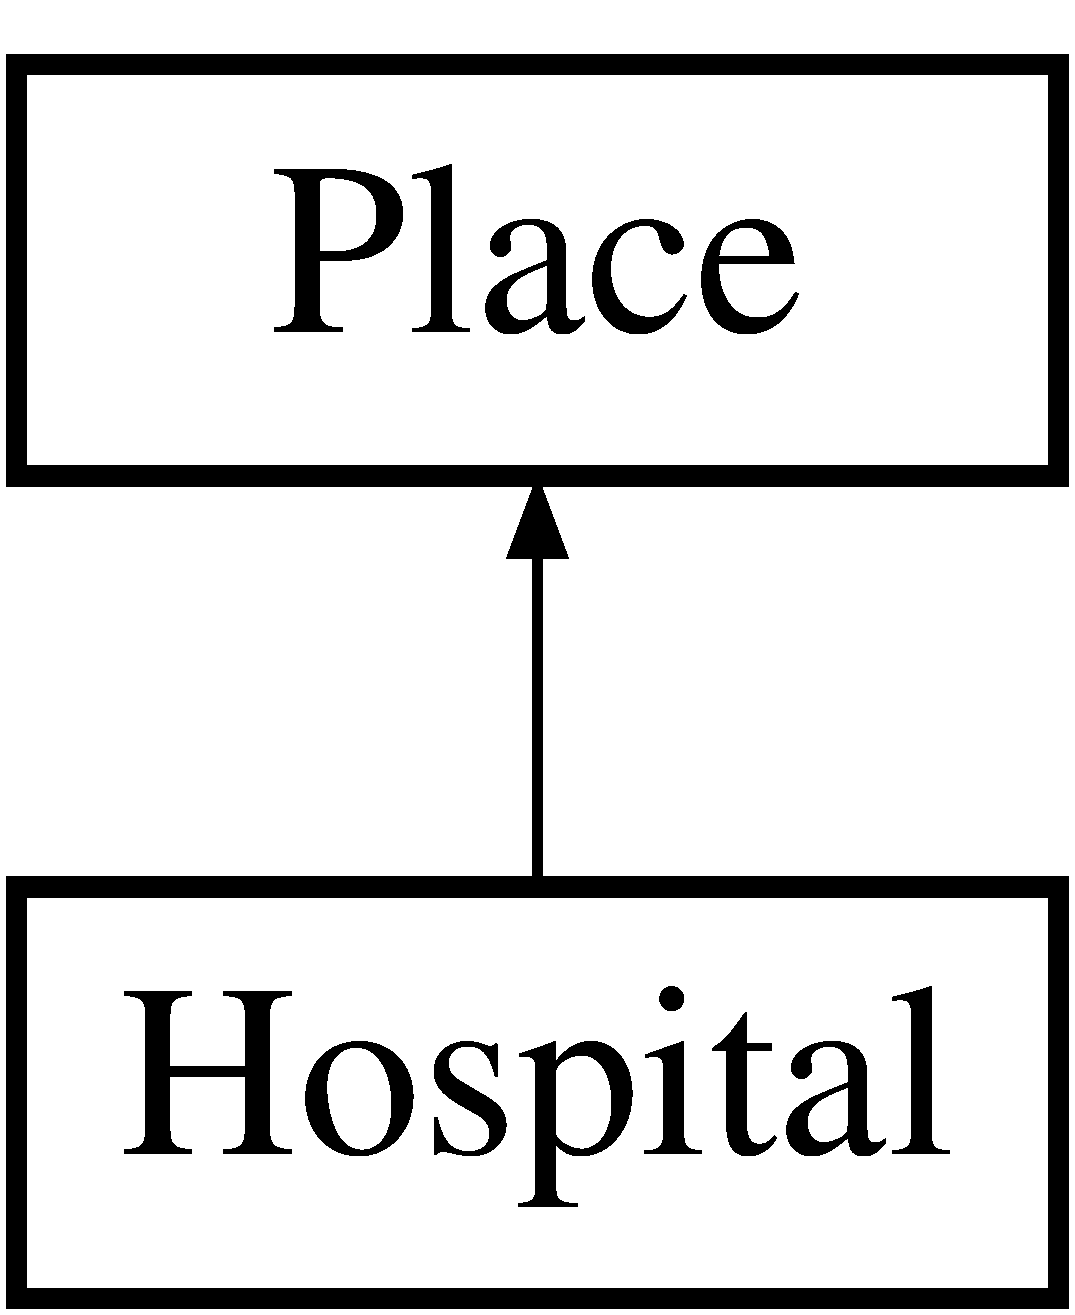
\includegraphics[height=2.000000cm]{classHospital}
\end{center}
\end{figure}
\subsection*{Public Member Functions}
\begin{DoxyCompactItemize}
\item 
\hyperlink{classHospital_ae76395fdb36d01f526cb962a13784fbd}{Hospital} ()=default
\begin{DoxyCompactList}\small\item\em Creates a \hyperlink{classHospital}{Hospital} object with default attributes. \end{DoxyCompactList}\item 
\hyperlink{classHospital_a9f0f34e37e3877d717e10e7e41af21f7}{Hospital} (const int hospital\+\_\+\+ID, const double xi, const double yi, const double severity\+\_\+cor, const std\+::map$<$ const std\+::string, const double $>$ betas)
\begin{DoxyCompactList}\small\item\em Creates a \hyperlink{classHospital}{Hospital} object. \end{DoxyCompactList}\item 
void \hyperlink{classHospital_a55c2f778b4aeb0f775bb1b45c147c7b8}{add\+\_\+exposed} (double inf\+\_\+var) override
\begin{DoxyCompactList}\small\item\em Include exposed employee contribution in the sum. \end{DoxyCompactList}\item 
void \hyperlink{classHospital_a68dc4af05fc1fbca3d5c48c835e8eb72}{add\+\_\+exposed\+\_\+patient} (double inf\+\_\+var)
\begin{DoxyCompactList}\small\item\em Include exposed contribution in the sum. \end{DoxyCompactList}\item 
void \hyperlink{classHospital_aa33d0902fa7c16cb04e0652cadfcd946}{add\+\_\+symptomatic\+\_\+patient} (double inf\+\_\+var)
\begin{DoxyCompactList}\small\item\em Include symptomatic contribution in the sum. \end{DoxyCompactList}\item 
void \hyperlink{classHospital_a501b5ff208e5cb612966f9200c6f359e}{add\+\_\+hospital\+\_\+tested} (double inf\+\_\+var)
\begin{DoxyCompactList}\small\item\em Include tested at hospital contribution in the sum. \end{DoxyCompactList}\item 
void \hyperlink{classHospital_a278812e4a6436ab49badb9e26a81be3f}{add\+\_\+exposed\+\_\+hospital\+\_\+tested} (double inf\+\_\+var)
\begin{DoxyCompactList}\small\item\em Include tested at hospital contribution in the sum. \end{DoxyCompactList}\item 
void \hyperlink{classHospital_a568e499510d128da61f39f3983fa20a8}{add\+\_\+hospitalized} (double inf\+\_\+var)
\begin{DoxyCompactList}\small\item\em Include hospitalized contribution in the sum. \end{DoxyCompactList}\item 
void \hyperlink{classHospital_a5a59a3e88cd740b32c8829f31a51f47c}{add\+\_\+hospitalized\+\_\+\+I\+CU} (double inf\+\_\+var)
\begin{DoxyCompactList}\small\item\em Include hospitalized in I\+CU contribution in the sum. \end{DoxyCompactList}\item 
void \hyperlink{classHospital_a2661ef21ce8561a28849d1be40e2ee50}{increase\+\_\+total\+\_\+tested} ()
\begin{DoxyCompactList}\small\item\em Increase number of tested at that time step. \end{DoxyCompactList}\item 
void \hyperlink{classHospital_a928d185dde78d0bce3034b7a138b472d}{reset\+\_\+contributions} () override
\begin{DoxyCompactList}\small\item\em Reset select variables of a place after transmission step. \end{DoxyCompactList}\item 
void \hyperlink{classHospital_ad87fc4a53e50a35489c9024892a7c9d6}{compute\+\_\+infected\+\_\+contribution} () override
\begin{DoxyCompactList}\small\item\em Contribution takes into account agents tested at current step. \end{DoxyCompactList}\item 
int \hyperlink{classHospital_ab7c68212de4e44986c8de732af160221}{get\+\_\+n\+\_\+tested} () const
\begin{DoxyCompactList}\small\item\em Returns number of \hyperlink{classFlu}{Flu} agents being tested in a hospital at that step. \end{DoxyCompactList}\item 
double \hyperlink{classHospital_a640cbef59ed726254579948f399d0e8e}{get\+\_\+lambda\+\_\+sum} () const
\begin{DoxyCompactList}\small\item\em Returns number of \hyperlink{classFlu}{Flu} agents being tested in a hospital at that step. \end{DoxyCompactList}\item 
void \hyperlink{classHospital_a3a1963886a9974663c2a3e82817f1a2b}{print\+\_\+basic} (std\+::ostream \&where) const override
\begin{DoxyCompactList}\small\item\em Save information about a \hyperlink{classHospital}{Hospital} object. \end{DoxyCompactList}\end{DoxyCompactItemize}
\subsection*{Additional Inherited Members}


\subsection{Constructor \& Destructor Documentation}
\mbox{\Hypertarget{classHospital_ae76395fdb36d01f526cb962a13784fbd}\label{classHospital_ae76395fdb36d01f526cb962a13784fbd}} 
\index{Hospital@{Hospital}!Hospital@{Hospital}}
\index{Hospital@{Hospital}!Hospital@{Hospital}}
\subsubsection{\texorpdfstring{Hospital()}{Hospital()}\hspace{0.1cm}{\footnotesize\ttfamily [1/2]}}
{\footnotesize\ttfamily Hospital\+::\+Hospital (\begin{DoxyParamCaption}{ }\end{DoxyParamCaption})\hspace{0.3cm}{\ttfamily [default]}}



Creates a \hyperlink{classHospital}{Hospital} object with default attributes. 

\mbox{\Hypertarget{classHospital_a9f0f34e37e3877d717e10e7e41af21f7}\label{classHospital_a9f0f34e37e3877d717e10e7e41af21f7}} 
\index{Hospital@{Hospital}!Hospital@{Hospital}}
\index{Hospital@{Hospital}!Hospital@{Hospital}}
\subsubsection{\texorpdfstring{Hospital()}{Hospital()}\hspace{0.1cm}{\footnotesize\ttfamily [2/2]}}
{\footnotesize\ttfamily Hospital\+::\+Hospital (\begin{DoxyParamCaption}\item[{const int}]{hospital\+\_\+\+ID,  }\item[{const double}]{xi,  }\item[{const double}]{yi,  }\item[{const double}]{severity\+\_\+cor,  }\item[{const std\+::map$<$ const std\+::string, const double $>$}]{betas }\end{DoxyParamCaption})\hspace{0.3cm}{\ttfamily [inline]}}



Creates a \hyperlink{classHospital}{Hospital} object. 

\hyperlink{classHospital}{Hospital} with custom ID, location, and infection parameters


\begin{DoxyParams}{Parameters}
{\em hospital\+\_\+\+ID} & -\/ ID of the hospital \\
\hline
{\em xi} & -\/ x coordinate of the hospital \\
\hline
{\em yi} & -\/ y coordinate of the hospital \\
\hline
{\em severity\+\_\+cor} & -\/ severity correction for symptomatic \\
\hline
{\em betas} & -\/ map of infection transmission rates, 1/time; name \+: value \\
\hline
\end{DoxyParams}


\subsection{Member Function Documentation}
\mbox{\Hypertarget{classHospital_a55c2f778b4aeb0f775bb1b45c147c7b8}\label{classHospital_a55c2f778b4aeb0f775bb1b45c147c7b8}} 
\index{Hospital@{Hospital}!add\+\_\+exposed@{add\+\_\+exposed}}
\index{add\+\_\+exposed@{add\+\_\+exposed}!Hospital@{Hospital}}
\subsubsection{\texorpdfstring{add\+\_\+exposed()}{add\_exposed()}}
{\footnotesize\ttfamily void Hospital\+::add\+\_\+exposed (\begin{DoxyParamCaption}\item[{double}]{inf\+\_\+var }\end{DoxyParamCaption})\hspace{0.3cm}{\ttfamily [inline]}, {\ttfamily [override]}, {\ttfamily [virtual]}}



Include exposed employee contribution in the sum. 


\begin{DoxyParams}{Parameters}
{\em inf\+\_\+var} & -\/ agent infectiousness variability factor \\
\hline
\end{DoxyParams}


Reimplemented from \hyperlink{classPlace_a96444ff0aa08a921598d0afb9c00cec8}{Place}.

\mbox{\Hypertarget{classHospital_a278812e4a6436ab49badb9e26a81be3f}\label{classHospital_a278812e4a6436ab49badb9e26a81be3f}} 
\index{Hospital@{Hospital}!add\+\_\+exposed\+\_\+hospital\+\_\+tested@{add\+\_\+exposed\+\_\+hospital\+\_\+tested}}
\index{add\+\_\+exposed\+\_\+hospital\+\_\+tested@{add\+\_\+exposed\+\_\+hospital\+\_\+tested}!Hospital@{Hospital}}
\subsubsection{\texorpdfstring{add\+\_\+exposed\+\_\+hospital\+\_\+tested()}{add\_exposed\_hospital\_tested()}}
{\footnotesize\ttfamily void Hospital\+::add\+\_\+exposed\+\_\+hospital\+\_\+tested (\begin{DoxyParamCaption}\item[{double}]{inf\+\_\+var }\end{DoxyParamCaption})\hspace{0.3cm}{\ttfamily [inline]}}



Include tested at hospital contribution in the sum. 


\begin{DoxyParams}{Parameters}
{\em inf\+\_\+var} & -\/ agent infectiousness variability factor \\
\hline
\end{DoxyParams}
\mbox{\Hypertarget{classHospital_a68dc4af05fc1fbca3d5c48c835e8eb72}\label{classHospital_a68dc4af05fc1fbca3d5c48c835e8eb72}} 
\index{Hospital@{Hospital}!add\+\_\+exposed\+\_\+patient@{add\+\_\+exposed\+\_\+patient}}
\index{add\+\_\+exposed\+\_\+patient@{add\+\_\+exposed\+\_\+patient}!Hospital@{Hospital}}
\subsubsection{\texorpdfstring{add\+\_\+exposed\+\_\+patient()}{add\_exposed\_patient()}}
{\footnotesize\ttfamily void Hospital\+::add\+\_\+exposed\+\_\+patient (\begin{DoxyParamCaption}\item[{double}]{inf\+\_\+var }\end{DoxyParamCaption})\hspace{0.3cm}{\ttfamily [inline]}}



Include exposed contribution in the sum. 


\begin{DoxyParams}{Parameters}
{\em inf\+\_\+var} & -\/ agent infectiousness variability factor \\
\hline
\end{DoxyParams}
\mbox{\Hypertarget{classHospital_a501b5ff208e5cb612966f9200c6f359e}\label{classHospital_a501b5ff208e5cb612966f9200c6f359e}} 
\index{Hospital@{Hospital}!add\+\_\+hospital\+\_\+tested@{add\+\_\+hospital\+\_\+tested}}
\index{add\+\_\+hospital\+\_\+tested@{add\+\_\+hospital\+\_\+tested}!Hospital@{Hospital}}
\subsubsection{\texorpdfstring{add\+\_\+hospital\+\_\+tested()}{add\_hospital\_tested()}}
{\footnotesize\ttfamily void Hospital\+::add\+\_\+hospital\+\_\+tested (\begin{DoxyParamCaption}\item[{double}]{inf\+\_\+var }\end{DoxyParamCaption})\hspace{0.3cm}{\ttfamily [inline]}}



Include tested at hospital contribution in the sum. 


\begin{DoxyParams}{Parameters}
{\em inf\+\_\+var} & -\/ agent infectiousness variability factor \\
\hline
\end{DoxyParams}
\mbox{\Hypertarget{classHospital_a568e499510d128da61f39f3983fa20a8}\label{classHospital_a568e499510d128da61f39f3983fa20a8}} 
\index{Hospital@{Hospital}!add\+\_\+hospitalized@{add\+\_\+hospitalized}}
\index{add\+\_\+hospitalized@{add\+\_\+hospitalized}!Hospital@{Hospital}}
\subsubsection{\texorpdfstring{add\+\_\+hospitalized()}{add\_hospitalized()}}
{\footnotesize\ttfamily void Hospital\+::add\+\_\+hospitalized (\begin{DoxyParamCaption}\item[{double}]{inf\+\_\+var }\end{DoxyParamCaption})\hspace{0.3cm}{\ttfamily [inline]}}



Include hospitalized contribution in the sum. 


\begin{DoxyParams}{Parameters}
{\em inf\+\_\+var} & -\/ agent infectiousness variability factor \\
\hline
\end{DoxyParams}
\mbox{\Hypertarget{classHospital_a5a59a3e88cd740b32c8829f31a51f47c}\label{classHospital_a5a59a3e88cd740b32c8829f31a51f47c}} 
\index{Hospital@{Hospital}!add\+\_\+hospitalized\+\_\+\+I\+CU@{add\+\_\+hospitalized\+\_\+\+I\+CU}}
\index{add\+\_\+hospitalized\+\_\+\+I\+CU@{add\+\_\+hospitalized\+\_\+\+I\+CU}!Hospital@{Hospital}}
\subsubsection{\texorpdfstring{add\+\_\+hospitalized\+\_\+\+I\+C\+U()}{add\_hospitalized\_ICU()}}
{\footnotesize\ttfamily void Hospital\+::add\+\_\+hospitalized\+\_\+\+I\+CU (\begin{DoxyParamCaption}\item[{double}]{inf\+\_\+var }\end{DoxyParamCaption})\hspace{0.3cm}{\ttfamily [inline]}}



Include hospitalized in I\+CU contribution in the sum. 


\begin{DoxyParams}{Parameters}
{\em inf\+\_\+var} & -\/ agent infectiousness variability factor \\
\hline
\end{DoxyParams}
\mbox{\Hypertarget{classHospital_aa33d0902fa7c16cb04e0652cadfcd946}\label{classHospital_aa33d0902fa7c16cb04e0652cadfcd946}} 
\index{Hospital@{Hospital}!add\+\_\+symptomatic\+\_\+patient@{add\+\_\+symptomatic\+\_\+patient}}
\index{add\+\_\+symptomatic\+\_\+patient@{add\+\_\+symptomatic\+\_\+patient}!Hospital@{Hospital}}
\subsubsection{\texorpdfstring{add\+\_\+symptomatic\+\_\+patient()}{add\_symptomatic\_patient()}}
{\footnotesize\ttfamily void Hospital\+::add\+\_\+symptomatic\+\_\+patient (\begin{DoxyParamCaption}\item[{double}]{inf\+\_\+var }\end{DoxyParamCaption})\hspace{0.3cm}{\ttfamily [inline]}}



Include symptomatic contribution in the sum. 


\begin{DoxyParams}{Parameters}
{\em inf\+\_\+var} & -\/ agent infectiousness variability factor \\
\hline
\end{DoxyParams}
\mbox{\Hypertarget{classHospital_ad87fc4a53e50a35489c9024892a7c9d6}\label{classHospital_ad87fc4a53e50a35489c9024892a7c9d6}} 
\index{Hospital@{Hospital}!compute\+\_\+infected\+\_\+contribution@{compute\+\_\+infected\+\_\+contribution}}
\index{compute\+\_\+infected\+\_\+contribution@{compute\+\_\+infected\+\_\+contribution}!Hospital@{Hospital}}
\subsubsection{\texorpdfstring{compute\+\_\+infected\+\_\+contribution()}{compute\_infected\_contribution()}}
{\footnotesize\ttfamily void Hospital\+::compute\+\_\+infected\+\_\+contribution (\begin{DoxyParamCaption}{ }\end{DoxyParamCaption})\hspace{0.3cm}{\ttfamily [override]}, {\ttfamily [virtual]}}



Contribution takes into account agents tested at current step. 



Reimplemented from \hyperlink{classPlace_aeb4c561e8bc4e1ae7186baed6ef1aa47}{Place}.

\mbox{\Hypertarget{classHospital_a640cbef59ed726254579948f399d0e8e}\label{classHospital_a640cbef59ed726254579948f399d0e8e}} 
\index{Hospital@{Hospital}!get\+\_\+lambda\+\_\+sum@{get\+\_\+lambda\+\_\+sum}}
\index{get\+\_\+lambda\+\_\+sum@{get\+\_\+lambda\+\_\+sum}!Hospital@{Hospital}}
\subsubsection{\texorpdfstring{get\+\_\+lambda\+\_\+sum()}{get\_lambda\_sum()}}
{\footnotesize\ttfamily double Hospital\+::get\+\_\+lambda\+\_\+sum (\begin{DoxyParamCaption}{ }\end{DoxyParamCaption}) const\hspace{0.3cm}{\ttfamily [inline]}}



Returns number of \hyperlink{classFlu}{Flu} agents being tested in a hospital at that step. 

\mbox{\Hypertarget{classHospital_ab7c68212de4e44986c8de732af160221}\label{classHospital_ab7c68212de4e44986c8de732af160221}} 
\index{Hospital@{Hospital}!get\+\_\+n\+\_\+tested@{get\+\_\+n\+\_\+tested}}
\index{get\+\_\+n\+\_\+tested@{get\+\_\+n\+\_\+tested}!Hospital@{Hospital}}
\subsubsection{\texorpdfstring{get\+\_\+n\+\_\+tested()}{get\_n\_tested()}}
{\footnotesize\ttfamily int Hospital\+::get\+\_\+n\+\_\+tested (\begin{DoxyParamCaption}{ }\end{DoxyParamCaption}) const\hspace{0.3cm}{\ttfamily [inline]}}



Returns number of \hyperlink{classFlu}{Flu} agents being tested in a hospital at that step. 

\mbox{\Hypertarget{classHospital_a2661ef21ce8561a28849d1be40e2ee50}\label{classHospital_a2661ef21ce8561a28849d1be40e2ee50}} 
\index{Hospital@{Hospital}!increase\+\_\+total\+\_\+tested@{increase\+\_\+total\+\_\+tested}}
\index{increase\+\_\+total\+\_\+tested@{increase\+\_\+total\+\_\+tested}!Hospital@{Hospital}}
\subsubsection{\texorpdfstring{increase\+\_\+total\+\_\+tested()}{increase\_total\_tested()}}
{\footnotesize\ttfamily void Hospital\+::increase\+\_\+total\+\_\+tested (\begin{DoxyParamCaption}{ }\end{DoxyParamCaption})\hspace{0.3cm}{\ttfamily [inline]}}



Increase number of tested at that time step. 

\mbox{\Hypertarget{classHospital_a3a1963886a9974663c2a3e82817f1a2b}\label{classHospital_a3a1963886a9974663c2a3e82817f1a2b}} 
\index{Hospital@{Hospital}!print\+\_\+basic@{print\+\_\+basic}}
\index{print\+\_\+basic@{print\+\_\+basic}!Hospital@{Hospital}}
\subsubsection{\texorpdfstring{print\+\_\+basic()}{print\_basic()}}
{\footnotesize\ttfamily void Hospital\+::print\+\_\+basic (\begin{DoxyParamCaption}\item[{std\+::ostream \&}]{where }\end{DoxyParamCaption}) const\hspace{0.3cm}{\ttfamily [override]}, {\ttfamily [virtual]}}



Save information about a \hyperlink{classHospital}{Hospital} object. 

Saves to a file, everything but detailed agent information; order is ID $\vert$ x $\vert$ y $\vert$ number of agents $\vert$ number of infected agents $\vert$ ck $\vert$ beta\+\_\+1, 2, and 3 Delimiter is a space. 
\begin{DoxyParams}{Parameters}
{\em where} & -\/ output stream \\
\hline
\end{DoxyParams}


Reimplemented from \hyperlink{classPlace_a9aa7649e0b91c5f61a5f71e9ca808fe1}{Place}.

\mbox{\Hypertarget{classHospital_a928d185dde78d0bce3034b7a138b472d}\label{classHospital_a928d185dde78d0bce3034b7a138b472d}} 
\index{Hospital@{Hospital}!reset\+\_\+contributions@{reset\+\_\+contributions}}
\index{reset\+\_\+contributions@{reset\+\_\+contributions}!Hospital@{Hospital}}
\subsubsection{\texorpdfstring{reset\+\_\+contributions()}{reset\_contributions()}}
{\footnotesize\ttfamily void Hospital\+::reset\+\_\+contributions (\begin{DoxyParamCaption}{ }\end{DoxyParamCaption})\hspace{0.3cm}{\ttfamily [inline]}, {\ttfamily [override]}, {\ttfamily [virtual]}}



Reset select variables of a place after transmission step. 



Reimplemented from \hyperlink{classPlace_abc1e560ef8aaaad565ccceb9540e5bd8}{Place}.



The documentation for this class was generated from the following files\+:\begin{DoxyCompactItemize}
\item 
include/places/\hyperlink{hospital_8h}{hospital.\+h}\item 
src/places/\hyperlink{hospital_8cpp}{hospital.\+cpp}\end{DoxyCompactItemize}

\hypertarget{classHousehold}{}\section{Household Class Reference}
\label{classHousehold}\index{Household@{Household}}


{\ttfamily \#include $<$household.\+h$>$}

Inheritance diagram for Household\+:\begin{figure}[H]
\begin{center}
\leavevmode
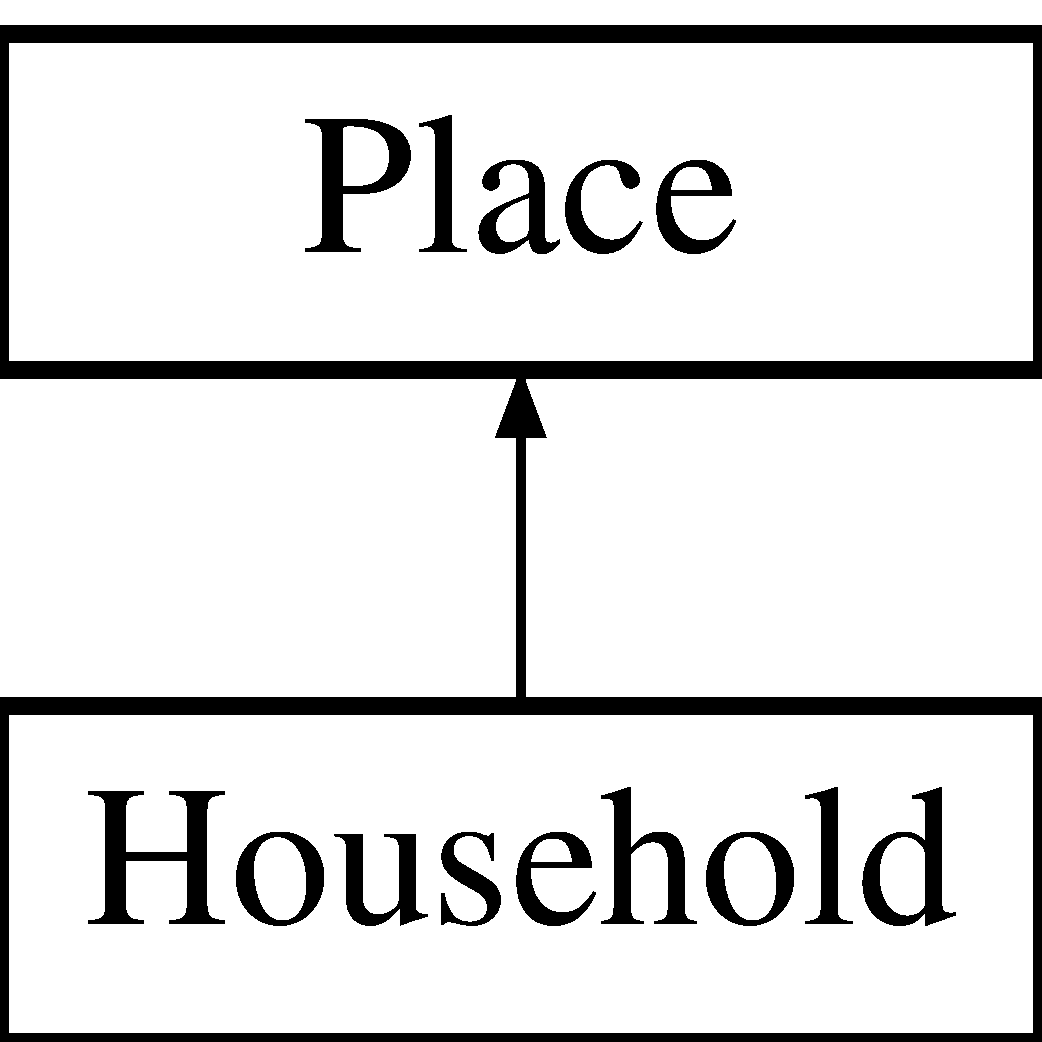
\includegraphics[height=2.000000cm]{classHousehold}
\end{center}
\end{figure}
\subsection*{Public Member Functions}
\begin{DoxyCompactItemize}
\item 
\hyperlink{classHousehold_a806512a49b82de676b263b47c7717391}{Household} ()=default
\begin{DoxyCompactList}\small\item\em Creates a \hyperlink{classHousehold}{Household} object with default attributes. \end{DoxyCompactList}\item 
\hyperlink{classHousehold_a0f96ac02e6cb0ecc7fd7a291af93c05e}{Household} (int house\+\_\+\+ID, double xi, double yi, const double alpha\+\_\+exp, const double severity\+\_\+cor, const double beta, const double betaih)
\begin{DoxyCompactList}\small\item\em Creates a \hyperlink{classHousehold}{Household} object. \end{DoxyCompactList}\item 
void \hyperlink{classHousehold_a9bf27cca25dea519945c8740b9793ff6}{print\+\_\+basic} (std\+::ostream \&where) const override
\begin{DoxyCompactList}\small\item\em Save information about a \hyperlink{classHousehold}{Household} object. \end{DoxyCompactList}\item 
void \hyperlink{classHousehold_ae063737d06a7a50aa9b780d7066c1c88}{compute\+\_\+infected\+\_\+contribution} () override
\begin{DoxyCompactList}\small\item\em Calculates and stores probability contribution of infected agents if any. \end{DoxyCompactList}\item 
void \hyperlink{classHousehold_ac2e5bde05d678a9ba853ddb9cf00ce3d}{add\+\_\+symptomatic\+\_\+home\+\_\+isolated} (double inf\+\_\+var)
\begin{DoxyCompactList}\small\item\em Include contribution of a symptomatic, home isolated agent in the sum. \end{DoxyCompactList}\item 
void \hyperlink{classHousehold_a28b12a90e592c6d3b1e9ac333e3d54d8}{add\+\_\+exposed\+\_\+home\+\_\+isolated} (double inf\+\_\+var)
\begin{DoxyCompactList}\small\item\em Include contribution of an exposed , home isolated agent in the sum. \end{DoxyCompactList}\end{DoxyCompactItemize}
\subsection*{Additional Inherited Members}


\subsection{Constructor \& Destructor Documentation}
\mbox{\Hypertarget{classHousehold_a806512a49b82de676b263b47c7717391}\label{classHousehold_a806512a49b82de676b263b47c7717391}} 
\index{Household@{Household}!Household@{Household}}
\index{Household@{Household}!Household@{Household}}
\subsubsection{\texorpdfstring{Household()}{Household()}\hspace{0.1cm}{\footnotesize\ttfamily [1/2]}}
{\footnotesize\ttfamily Household\+::\+Household (\begin{DoxyParamCaption}{ }\end{DoxyParamCaption})\hspace{0.3cm}{\ttfamily [default]}}



Creates a \hyperlink{classHousehold}{Household} object with default attributes. 

\mbox{\Hypertarget{classHousehold_a0f96ac02e6cb0ecc7fd7a291af93c05e}\label{classHousehold_a0f96ac02e6cb0ecc7fd7a291af93c05e}} 
\index{Household@{Household}!Household@{Household}}
\index{Household@{Household}!Household@{Household}}
\subsubsection{\texorpdfstring{Household()}{Household()}\hspace{0.1cm}{\footnotesize\ttfamily [2/2]}}
{\footnotesize\ttfamily Household\+::\+Household (\begin{DoxyParamCaption}\item[{int}]{house\+\_\+\+ID,  }\item[{double}]{xi,  }\item[{double}]{yi,  }\item[{const double}]{alpha\+\_\+exp,  }\item[{const double}]{severity\+\_\+cor,  }\item[{const double}]{beta,  }\item[{const double}]{betaih }\end{DoxyParamCaption})\hspace{0.3cm}{\ttfamily [inline]}}



Creates a \hyperlink{classHousehold}{Household} object. 

\hyperlink{classHousehold}{Household} with custom ID, location, and infection parameters


\begin{DoxyParams}{Parameters}
{\em house\+\_\+\+ID} & -\/ ID of the household \\
\hline
{\em xi} & -\/ x coordinate of the household \\
\hline
{\em yi} & -\/ y coordinate of the household \\
\hline
{\em alpha\+\_\+exp} & -\/ household size correction \\
\hline
{\em severity\+\_\+cor} & -\/ severity correction for symptomatic \\
\hline
{\em beta} & -\/ infection transmission rate, 1/time \\
\hline
{\em betaih} & -\/ infection transmission rate for home isolated, 1/time \\
\hline
\end{DoxyParams}


\subsection{Member Function Documentation}
\mbox{\Hypertarget{classHousehold_a28b12a90e592c6d3b1e9ac333e3d54d8}\label{classHousehold_a28b12a90e592c6d3b1e9ac333e3d54d8}} 
\index{Household@{Household}!add\+\_\+exposed\+\_\+home\+\_\+isolated@{add\+\_\+exposed\+\_\+home\+\_\+isolated}}
\index{add\+\_\+exposed\+\_\+home\+\_\+isolated@{add\+\_\+exposed\+\_\+home\+\_\+isolated}!Household@{Household}}
\subsubsection{\texorpdfstring{add\+\_\+exposed\+\_\+home\+\_\+isolated()}{add\_exposed\_home\_isolated()}}
{\footnotesize\ttfamily void Household\+::add\+\_\+exposed\+\_\+home\+\_\+isolated (\begin{DoxyParamCaption}\item[{double}]{inf\+\_\+var }\end{DoxyParamCaption})\hspace{0.3cm}{\ttfamily [inline]}}



Include contribution of an exposed , home isolated agent in the sum. 


\begin{DoxyParams}{Parameters}
{\em inf\+\_\+var} & -\/ agent infectiousness variability factor \\
\hline
\end{DoxyParams}
\mbox{\Hypertarget{classHousehold_ac2e5bde05d678a9ba853ddb9cf00ce3d}\label{classHousehold_ac2e5bde05d678a9ba853ddb9cf00ce3d}} 
\index{Household@{Household}!add\+\_\+symptomatic\+\_\+home\+\_\+isolated@{add\+\_\+symptomatic\+\_\+home\+\_\+isolated}}
\index{add\+\_\+symptomatic\+\_\+home\+\_\+isolated@{add\+\_\+symptomatic\+\_\+home\+\_\+isolated}!Household@{Household}}
\subsubsection{\texorpdfstring{add\+\_\+symptomatic\+\_\+home\+\_\+isolated()}{add\_symptomatic\_home\_isolated()}}
{\footnotesize\ttfamily void Household\+::add\+\_\+symptomatic\+\_\+home\+\_\+isolated (\begin{DoxyParamCaption}\item[{double}]{inf\+\_\+var }\end{DoxyParamCaption})\hspace{0.3cm}{\ttfamily [inline]}}



Include contribution of a symptomatic, home isolated agent in the sum. 


\begin{DoxyParams}{Parameters}
{\em inf\+\_\+var} & -\/ agent infectiousness variability factor \\
\hline
\end{DoxyParams}
\mbox{\Hypertarget{classHousehold_ae063737d06a7a50aa9b780d7066c1c88}\label{classHousehold_ae063737d06a7a50aa9b780d7066c1c88}} 
\index{Household@{Household}!compute\+\_\+infected\+\_\+contribution@{compute\+\_\+infected\+\_\+contribution}}
\index{compute\+\_\+infected\+\_\+contribution@{compute\+\_\+infected\+\_\+contribution}!Household@{Household}}
\subsubsection{\texorpdfstring{compute\+\_\+infected\+\_\+contribution()}{compute\_infected\_contribution()}}
{\footnotesize\ttfamily void Household\+::compute\+\_\+infected\+\_\+contribution (\begin{DoxyParamCaption}{ }\end{DoxyParamCaption})\hspace{0.3cm}{\ttfamily [override]}, {\ttfamily [virtual]}}



Calculates and stores probability contribution of infected agents if any. 


\begin{DoxyParams}{Parameters}
{\em infection} & -\/ infection object class instance \\
\hline
\end{DoxyParams}


Reimplemented from \hyperlink{classPlace_aeb4c561e8bc4e1ae7186baed6ef1aa47}{Place}.

\mbox{\Hypertarget{classHousehold_a9bf27cca25dea519945c8740b9793ff6}\label{classHousehold_a9bf27cca25dea519945c8740b9793ff6}} 
\index{Household@{Household}!print\+\_\+basic@{print\+\_\+basic}}
\index{print\+\_\+basic@{print\+\_\+basic}!Household@{Household}}
\subsubsection{\texorpdfstring{print\+\_\+basic()}{print\_basic()}}
{\footnotesize\ttfamily void Household\+::print\+\_\+basic (\begin{DoxyParamCaption}\item[{std\+::ostream \&}]{where }\end{DoxyParamCaption}) const\hspace{0.3cm}{\ttfamily [override]}, {\ttfamily [virtual]}}



Save information about a \hyperlink{classHousehold}{Household} object. 

Saves to a file, everything but detailed agent information; order is ID $\vert$ x $\vert$ y $\vert$ number of agents $\vert$ number of infected agents $\vert$ ck $\vert$ beta\+\_\+j $\vert$ alpha Delimiter is a space.


\begin{DoxyParams}{Parameters}
{\em where} & -\/ output stream \\
\hline
\end{DoxyParams}


Reimplemented from \hyperlink{classPlace_a9aa7649e0b91c5f61a5f71e9ca808fe1}{Place}.



The documentation for this class was generated from the following files\+:\begin{DoxyCompactItemize}
\item 
include/places/\hyperlink{household_8h}{household.\+h}\item 
src/places/\hyperlink{household_8cpp}{household.\+cpp}\end{DoxyCompactItemize}

\hypertarget{classHspEmployeeStatesManager}{}\section{Hsp\+Employee\+States\+Manager Class Reference}
\label{classHspEmployeeStatesManager}\index{Hsp\+Employee\+States\+Manager@{Hsp\+Employee\+States\+Manager}}


{\ttfamily \#include $<$hsp\+\_\+employee\+\_\+states\+\_\+manager.\+h$>$}

\subsection*{Public Member Functions}
\begin{DoxyCompactItemize}
\item 
\hyperlink{classHspEmployeeStatesManager_a76b1f4aa0c3bc03c072878c5678ea420}{Hsp\+Employee\+States\+Manager} ()=default
\item 
void \hyperlink{classHspEmployeeStatesManager_a4fea72f10a69fe01212a847b43969f3e}{set\+\_\+susceptible\+\_\+to\+\_\+exposed} (\hyperlink{classAgent}{Agent} \&agent)
\begin{DoxyCompactList}\small\item\em Set all states for transition from susceptible to exposed. \end{DoxyCompactList}\item 
void \hyperlink{classHspEmployeeStatesManager_aa745324359627d4497c255be7b9615e1}{set\+\_\+susceptible\+\_\+to\+\_\+exposed\+\_\+never\+\_\+symptomatic} (\hyperlink{classAgent}{Agent} \&agent)
\begin{DoxyCompactList}\small\item\em Set all states for transition from susceptible to exposed that will never become symptomatic. \end{DoxyCompactList}\item 
void \hyperlink{classHspEmployeeStatesManager_a7f53c872e0297fae9a9f8ef78d861682}{set\+\_\+exposed\+\_\+never\+\_\+symptomatic\+\_\+to\+\_\+removed} (\hyperlink{classAgent}{Agent} \&agent)
\begin{DoxyCompactList}\small\item\em Set exposed that never developed symptoms to removed. \end{DoxyCompactList}\item 
void \hyperlink{classHspEmployeeStatesManager_a0d0d4d403644011774c738435a226ea2}{set\+\_\+exposed\+\_\+to\+\_\+symptomatic} (\hyperlink{classAgent}{Agent} \&agent)
\begin{DoxyCompactList}\small\item\em Set all states for transition from exposed to general symptomatic. \end{DoxyCompactList}\item 
void \hyperlink{classHspEmployeeStatesManager_a8496e09c1ad539dcfc4b9fc64ba86fbf}{set\+\_\+dying\+\_\+symptomatic} (\hyperlink{classAgent}{Agent} \&agent)
\begin{DoxyCompactList}\small\item\em Set all states relevant to agent that will die. \end{DoxyCompactList}\item 
void \hyperlink{classHspEmployeeStatesManager_a3ed9fedc4e2b32d21d472463af5d3df5}{set\+\_\+recovering\+\_\+symptomatic} (\hyperlink{classAgent}{Agent} \&agent)
\begin{DoxyCompactList}\small\item\em Set all states relevant to agent that will recover. \end{DoxyCompactList}\item 
void \hyperlink{classHspEmployeeStatesManager_a76dfcc6cd9c617f881bc44984a673174}{set\+\_\+waiting\+\_\+for\+\_\+test\+\_\+in\+\_\+hospital} (\hyperlink{classAgent}{Agent} \&agent)
\begin{DoxyCompactList}\small\item\em Set testing in hospital, initial state. \end{DoxyCompactList}\item 
void \hyperlink{classHspEmployeeStatesManager_aca27d50807561a44dd4a96eba69dc2bf}{set\+\_\+exposed\+\_\+waiting\+\_\+for\+\_\+test\+\_\+in\+\_\+hospital} (\hyperlink{classAgent}{Agent} \&agent)
\begin{DoxyCompactList}\small\item\em Set testing in hospital for exposed, initial state. \end{DoxyCompactList}\item 
void \hyperlink{classHspEmployeeStatesManager_a4b0f847d5e9ce5e1b48813ba506cfe36}{set\+\_\+tested\+\_\+to\+\_\+awaiting\+\_\+results} (\hyperlink{classAgent}{Agent} \&agent)
\begin{DoxyCompactList}\small\item\em Set all states for just tested. \end{DoxyCompactList}\item 
void \hyperlink{classHspEmployeeStatesManager_aaefccb28d50be6a89b20255779275520}{set\+\_\+tested\+\_\+false\+\_\+negative} (\hyperlink{classAgent}{Agent} \&agent)
\begin{DoxyCompactList}\small\item\em Set all states for transition from tested to false negative. \end{DoxyCompactList}\item 
void \hyperlink{classHspEmployeeStatesManager_aa5f8881bc33d8b92965d828295cc5251}{set\+\_\+icu\+\_\+dying} (\hyperlink{classAgent}{Agent} \&agent)
\begin{DoxyCompactList}\small\item\em States for hospitalized, I\+CU -\/ dying. \end{DoxyCompactList}\item 
void \hyperlink{classHspEmployeeStatesManager_acb3bbc5680fafac83634f93975d6f684}{set\+\_\+icu\+\_\+recovering} (\hyperlink{classAgent}{Agent} \&agent)
\begin{DoxyCompactList}\small\item\em States for hospitalized, I\+CU -\/ recovering. \end{DoxyCompactList}\item 
void \hyperlink{classHspEmployeeStatesManager_a33035540117578d7a090458c89a7cf33}{set\+\_\+hospitalized} (\hyperlink{classAgent}{Agent} \&agent)
\begin{DoxyCompactList}\small\item\em States for hospitalized. \end{DoxyCompactList}\item 
void \hyperlink{classHspEmployeeStatesManager_ab41695ae171267f0aac57a1d7ddfe154}{set\+\_\+home\+\_\+isolation} (\hyperlink{classAgent}{Agent} \&agent)
\begin{DoxyCompactList}\small\item\em States for isolated at home. \end{DoxyCompactList}\item 
void \hyperlink{classHspEmployeeStatesManager_a81c114346fa3ca81ed104ba2c5db9b49}{set\+\_\+any\+\_\+to\+\_\+removed} (\hyperlink{classAgent}{Agent} \&agent)
\begin{DoxyCompactList}\small\item\em Set all removed related states. \end{DoxyCompactList}\item 
void \hyperlink{classHspEmployeeStatesManager_a3b9a2c2ac3b20777c5c7d75dc6f9c002}{set\+\_\+tested\+\_\+negative} (\hyperlink{classAgent}{Agent} \&agent)
\begin{DoxyCompactList}\small\item\em States for negative. \end{DoxyCompactList}\item 
void \hyperlink{classHspEmployeeStatesManager_a8a648a456fb00140b8362201e034a05a}{reset\+\_\+returning\+\_\+flu} (\hyperlink{classAgent}{Agent} \&agent)
\begin{DoxyCompactList}\small\item\em Reset flags for flu that is back to susceptible from IH. \end{DoxyCompactList}\end{DoxyCompactItemize}


\subsection{Constructor \& Destructor Documentation}
\mbox{\Hypertarget{classHspEmployeeStatesManager_a76b1f4aa0c3bc03c072878c5678ea420}\label{classHspEmployeeStatesManager_a76b1f4aa0c3bc03c072878c5678ea420}} 
\index{Hsp\+Employee\+States\+Manager@{Hsp\+Employee\+States\+Manager}!Hsp\+Employee\+States\+Manager@{Hsp\+Employee\+States\+Manager}}
\index{Hsp\+Employee\+States\+Manager@{Hsp\+Employee\+States\+Manager}!Hsp\+Employee\+States\+Manager@{Hsp\+Employee\+States\+Manager}}
\subsubsection{\texorpdfstring{Hsp\+Employee\+States\+Manager()}{HspEmployeeStatesManager()}}
{\footnotesize\ttfamily Hsp\+Employee\+States\+Manager\+::\+Hsp\+Employee\+States\+Manager (\begin{DoxyParamCaption}{ }\end{DoxyParamCaption})\hspace{0.3cm}{\ttfamily [default]}}



\subsection{Member Function Documentation}
\mbox{\Hypertarget{classHspEmployeeStatesManager_a8a648a456fb00140b8362201e034a05a}\label{classHspEmployeeStatesManager_a8a648a456fb00140b8362201e034a05a}} 
\index{Hsp\+Employee\+States\+Manager@{Hsp\+Employee\+States\+Manager}!reset\+\_\+returning\+\_\+flu@{reset\+\_\+returning\+\_\+flu}}
\index{reset\+\_\+returning\+\_\+flu@{reset\+\_\+returning\+\_\+flu}!Hsp\+Employee\+States\+Manager@{Hsp\+Employee\+States\+Manager}}
\subsubsection{\texorpdfstring{reset\+\_\+returning\+\_\+flu()}{reset\_returning\_flu()}}
{\footnotesize\ttfamily void Hsp\+Employee\+States\+Manager\+::reset\+\_\+returning\+\_\+flu (\begin{DoxyParamCaption}\item[{\hyperlink{classAgent}{Agent} \&}]{agent }\end{DoxyParamCaption})}



Reset flags for flu that is back to susceptible from IH. 

\mbox{\Hypertarget{classHspEmployeeStatesManager_a81c114346fa3ca81ed104ba2c5db9b49}\label{classHspEmployeeStatesManager_a81c114346fa3ca81ed104ba2c5db9b49}} 
\index{Hsp\+Employee\+States\+Manager@{Hsp\+Employee\+States\+Manager}!set\+\_\+any\+\_\+to\+\_\+removed@{set\+\_\+any\+\_\+to\+\_\+removed}}
\index{set\+\_\+any\+\_\+to\+\_\+removed@{set\+\_\+any\+\_\+to\+\_\+removed}!Hsp\+Employee\+States\+Manager@{Hsp\+Employee\+States\+Manager}}
\subsubsection{\texorpdfstring{set\+\_\+any\+\_\+to\+\_\+removed()}{set\_any\_to\_removed()}}
{\footnotesize\ttfamily void Hsp\+Employee\+States\+Manager\+::set\+\_\+any\+\_\+to\+\_\+removed (\begin{DoxyParamCaption}\item[{\hyperlink{classAgent}{Agent} \&}]{agent }\end{DoxyParamCaption})}



Set all removed related states. 

\mbox{\Hypertarget{classHspEmployeeStatesManager_a8496e09c1ad539dcfc4b9fc64ba86fbf}\label{classHspEmployeeStatesManager_a8496e09c1ad539dcfc4b9fc64ba86fbf}} 
\index{Hsp\+Employee\+States\+Manager@{Hsp\+Employee\+States\+Manager}!set\+\_\+dying\+\_\+symptomatic@{set\+\_\+dying\+\_\+symptomatic}}
\index{set\+\_\+dying\+\_\+symptomatic@{set\+\_\+dying\+\_\+symptomatic}!Hsp\+Employee\+States\+Manager@{Hsp\+Employee\+States\+Manager}}
\subsubsection{\texorpdfstring{set\+\_\+dying\+\_\+symptomatic()}{set\_dying\_symptomatic()}}
{\footnotesize\ttfamily void Hsp\+Employee\+States\+Manager\+::set\+\_\+dying\+\_\+symptomatic (\begin{DoxyParamCaption}\item[{\hyperlink{classAgent}{Agent} \&}]{agent }\end{DoxyParamCaption})}



Set all states relevant to agent that will die. 

\mbox{\Hypertarget{classHspEmployeeStatesManager_a7f53c872e0297fae9a9f8ef78d861682}\label{classHspEmployeeStatesManager_a7f53c872e0297fae9a9f8ef78d861682}} 
\index{Hsp\+Employee\+States\+Manager@{Hsp\+Employee\+States\+Manager}!set\+\_\+exposed\+\_\+never\+\_\+symptomatic\+\_\+to\+\_\+removed@{set\+\_\+exposed\+\_\+never\+\_\+symptomatic\+\_\+to\+\_\+removed}}
\index{set\+\_\+exposed\+\_\+never\+\_\+symptomatic\+\_\+to\+\_\+removed@{set\+\_\+exposed\+\_\+never\+\_\+symptomatic\+\_\+to\+\_\+removed}!Hsp\+Employee\+States\+Manager@{Hsp\+Employee\+States\+Manager}}
\subsubsection{\texorpdfstring{set\+\_\+exposed\+\_\+never\+\_\+symptomatic\+\_\+to\+\_\+removed()}{set\_exposed\_never\_symptomatic\_to\_removed()}}
{\footnotesize\ttfamily void Hsp\+Employee\+States\+Manager\+::set\+\_\+exposed\+\_\+never\+\_\+symptomatic\+\_\+to\+\_\+removed (\begin{DoxyParamCaption}\item[{\hyperlink{classAgent}{Agent} \&}]{agent }\end{DoxyParamCaption})}



Set exposed that never developed symptoms to removed. 

\mbox{\Hypertarget{classHspEmployeeStatesManager_a0d0d4d403644011774c738435a226ea2}\label{classHspEmployeeStatesManager_a0d0d4d403644011774c738435a226ea2}} 
\index{Hsp\+Employee\+States\+Manager@{Hsp\+Employee\+States\+Manager}!set\+\_\+exposed\+\_\+to\+\_\+symptomatic@{set\+\_\+exposed\+\_\+to\+\_\+symptomatic}}
\index{set\+\_\+exposed\+\_\+to\+\_\+symptomatic@{set\+\_\+exposed\+\_\+to\+\_\+symptomatic}!Hsp\+Employee\+States\+Manager@{Hsp\+Employee\+States\+Manager}}
\subsubsection{\texorpdfstring{set\+\_\+exposed\+\_\+to\+\_\+symptomatic()}{set\_exposed\_to\_symptomatic()}}
{\footnotesize\ttfamily void Hsp\+Employee\+States\+Manager\+::set\+\_\+exposed\+\_\+to\+\_\+symptomatic (\begin{DoxyParamCaption}\item[{\hyperlink{classAgent}{Agent} \&}]{agent }\end{DoxyParamCaption})}



Set all states for transition from exposed to general symptomatic. 

\mbox{\Hypertarget{classHspEmployeeStatesManager_aca27d50807561a44dd4a96eba69dc2bf}\label{classHspEmployeeStatesManager_aca27d50807561a44dd4a96eba69dc2bf}} 
\index{Hsp\+Employee\+States\+Manager@{Hsp\+Employee\+States\+Manager}!set\+\_\+exposed\+\_\+waiting\+\_\+for\+\_\+test\+\_\+in\+\_\+hospital@{set\+\_\+exposed\+\_\+waiting\+\_\+for\+\_\+test\+\_\+in\+\_\+hospital}}
\index{set\+\_\+exposed\+\_\+waiting\+\_\+for\+\_\+test\+\_\+in\+\_\+hospital@{set\+\_\+exposed\+\_\+waiting\+\_\+for\+\_\+test\+\_\+in\+\_\+hospital}!Hsp\+Employee\+States\+Manager@{Hsp\+Employee\+States\+Manager}}
\subsubsection{\texorpdfstring{set\+\_\+exposed\+\_\+waiting\+\_\+for\+\_\+test\+\_\+in\+\_\+hospital()}{set\_exposed\_waiting\_for\_test\_in\_hospital()}}
{\footnotesize\ttfamily void Hsp\+Employee\+States\+Manager\+::set\+\_\+exposed\+\_\+waiting\+\_\+for\+\_\+test\+\_\+in\+\_\+hospital (\begin{DoxyParamCaption}\item[{\hyperlink{classAgent}{Agent} \&}]{agent }\end{DoxyParamCaption})}



Set testing in hospital for exposed, initial state. 

\mbox{\Hypertarget{classHspEmployeeStatesManager_ab41695ae171267f0aac57a1d7ddfe154}\label{classHspEmployeeStatesManager_ab41695ae171267f0aac57a1d7ddfe154}} 
\index{Hsp\+Employee\+States\+Manager@{Hsp\+Employee\+States\+Manager}!set\+\_\+home\+\_\+isolation@{set\+\_\+home\+\_\+isolation}}
\index{set\+\_\+home\+\_\+isolation@{set\+\_\+home\+\_\+isolation}!Hsp\+Employee\+States\+Manager@{Hsp\+Employee\+States\+Manager}}
\subsubsection{\texorpdfstring{set\+\_\+home\+\_\+isolation()}{set\_home\_isolation()}}
{\footnotesize\ttfamily void Hsp\+Employee\+States\+Manager\+::set\+\_\+home\+\_\+isolation (\begin{DoxyParamCaption}\item[{\hyperlink{classAgent}{Agent} \&}]{agent }\end{DoxyParamCaption})}



States for isolated at home. 

\mbox{\Hypertarget{classHspEmployeeStatesManager_a33035540117578d7a090458c89a7cf33}\label{classHspEmployeeStatesManager_a33035540117578d7a090458c89a7cf33}} 
\index{Hsp\+Employee\+States\+Manager@{Hsp\+Employee\+States\+Manager}!set\+\_\+hospitalized@{set\+\_\+hospitalized}}
\index{set\+\_\+hospitalized@{set\+\_\+hospitalized}!Hsp\+Employee\+States\+Manager@{Hsp\+Employee\+States\+Manager}}
\subsubsection{\texorpdfstring{set\+\_\+hospitalized()}{set\_hospitalized()}}
{\footnotesize\ttfamily void Hsp\+Employee\+States\+Manager\+::set\+\_\+hospitalized (\begin{DoxyParamCaption}\item[{\hyperlink{classAgent}{Agent} \&}]{agent }\end{DoxyParamCaption})}



States for hospitalized. 

\mbox{\Hypertarget{classHspEmployeeStatesManager_aa5f8881bc33d8b92965d828295cc5251}\label{classHspEmployeeStatesManager_aa5f8881bc33d8b92965d828295cc5251}} 
\index{Hsp\+Employee\+States\+Manager@{Hsp\+Employee\+States\+Manager}!set\+\_\+icu\+\_\+dying@{set\+\_\+icu\+\_\+dying}}
\index{set\+\_\+icu\+\_\+dying@{set\+\_\+icu\+\_\+dying}!Hsp\+Employee\+States\+Manager@{Hsp\+Employee\+States\+Manager}}
\subsubsection{\texorpdfstring{set\+\_\+icu\+\_\+dying()}{set\_icu\_dying()}}
{\footnotesize\ttfamily void Hsp\+Employee\+States\+Manager\+::set\+\_\+icu\+\_\+dying (\begin{DoxyParamCaption}\item[{\hyperlink{classAgent}{Agent} \&}]{agent }\end{DoxyParamCaption})}



States for hospitalized, I\+CU -\/ dying. 

\mbox{\Hypertarget{classHspEmployeeStatesManager_acb3bbc5680fafac83634f93975d6f684}\label{classHspEmployeeStatesManager_acb3bbc5680fafac83634f93975d6f684}} 
\index{Hsp\+Employee\+States\+Manager@{Hsp\+Employee\+States\+Manager}!set\+\_\+icu\+\_\+recovering@{set\+\_\+icu\+\_\+recovering}}
\index{set\+\_\+icu\+\_\+recovering@{set\+\_\+icu\+\_\+recovering}!Hsp\+Employee\+States\+Manager@{Hsp\+Employee\+States\+Manager}}
\subsubsection{\texorpdfstring{set\+\_\+icu\+\_\+recovering()}{set\_icu\_recovering()}}
{\footnotesize\ttfamily void Hsp\+Employee\+States\+Manager\+::set\+\_\+icu\+\_\+recovering (\begin{DoxyParamCaption}\item[{\hyperlink{classAgent}{Agent} \&}]{agent }\end{DoxyParamCaption})}



States for hospitalized, I\+CU -\/ recovering. 

\mbox{\Hypertarget{classHspEmployeeStatesManager_a3ed9fedc4e2b32d21d472463af5d3df5}\label{classHspEmployeeStatesManager_a3ed9fedc4e2b32d21d472463af5d3df5}} 
\index{Hsp\+Employee\+States\+Manager@{Hsp\+Employee\+States\+Manager}!set\+\_\+recovering\+\_\+symptomatic@{set\+\_\+recovering\+\_\+symptomatic}}
\index{set\+\_\+recovering\+\_\+symptomatic@{set\+\_\+recovering\+\_\+symptomatic}!Hsp\+Employee\+States\+Manager@{Hsp\+Employee\+States\+Manager}}
\subsubsection{\texorpdfstring{set\+\_\+recovering\+\_\+symptomatic()}{set\_recovering\_symptomatic()}}
{\footnotesize\ttfamily void Hsp\+Employee\+States\+Manager\+::set\+\_\+recovering\+\_\+symptomatic (\begin{DoxyParamCaption}\item[{\hyperlink{classAgent}{Agent} \&}]{agent }\end{DoxyParamCaption})}



Set all states relevant to agent that will recover. 

\mbox{\Hypertarget{classHspEmployeeStatesManager_a4fea72f10a69fe01212a847b43969f3e}\label{classHspEmployeeStatesManager_a4fea72f10a69fe01212a847b43969f3e}} 
\index{Hsp\+Employee\+States\+Manager@{Hsp\+Employee\+States\+Manager}!set\+\_\+susceptible\+\_\+to\+\_\+exposed@{set\+\_\+susceptible\+\_\+to\+\_\+exposed}}
\index{set\+\_\+susceptible\+\_\+to\+\_\+exposed@{set\+\_\+susceptible\+\_\+to\+\_\+exposed}!Hsp\+Employee\+States\+Manager@{Hsp\+Employee\+States\+Manager}}
\subsubsection{\texorpdfstring{set\+\_\+susceptible\+\_\+to\+\_\+exposed()}{set\_susceptible\_to\_exposed()}}
{\footnotesize\ttfamily void Hsp\+Employee\+States\+Manager\+::set\+\_\+susceptible\+\_\+to\+\_\+exposed (\begin{DoxyParamCaption}\item[{\hyperlink{classAgent}{Agent} \&}]{agent }\end{DoxyParamCaption})}



Set all states for transition from susceptible to exposed. 

\mbox{\Hypertarget{classHspEmployeeStatesManager_aa745324359627d4497c255be7b9615e1}\label{classHspEmployeeStatesManager_aa745324359627d4497c255be7b9615e1}} 
\index{Hsp\+Employee\+States\+Manager@{Hsp\+Employee\+States\+Manager}!set\+\_\+susceptible\+\_\+to\+\_\+exposed\+\_\+never\+\_\+symptomatic@{set\+\_\+susceptible\+\_\+to\+\_\+exposed\+\_\+never\+\_\+symptomatic}}
\index{set\+\_\+susceptible\+\_\+to\+\_\+exposed\+\_\+never\+\_\+symptomatic@{set\+\_\+susceptible\+\_\+to\+\_\+exposed\+\_\+never\+\_\+symptomatic}!Hsp\+Employee\+States\+Manager@{Hsp\+Employee\+States\+Manager}}
\subsubsection{\texorpdfstring{set\+\_\+susceptible\+\_\+to\+\_\+exposed\+\_\+never\+\_\+symptomatic()}{set\_susceptible\_to\_exposed\_never\_symptomatic()}}
{\footnotesize\ttfamily void Hsp\+Employee\+States\+Manager\+::set\+\_\+susceptible\+\_\+to\+\_\+exposed\+\_\+never\+\_\+symptomatic (\begin{DoxyParamCaption}\item[{\hyperlink{classAgent}{Agent} \&}]{agent }\end{DoxyParamCaption})}



Set all states for transition from susceptible to exposed that will never become symptomatic. 

\mbox{\Hypertarget{classHspEmployeeStatesManager_aaefccb28d50be6a89b20255779275520}\label{classHspEmployeeStatesManager_aaefccb28d50be6a89b20255779275520}} 
\index{Hsp\+Employee\+States\+Manager@{Hsp\+Employee\+States\+Manager}!set\+\_\+tested\+\_\+false\+\_\+negative@{set\+\_\+tested\+\_\+false\+\_\+negative}}
\index{set\+\_\+tested\+\_\+false\+\_\+negative@{set\+\_\+tested\+\_\+false\+\_\+negative}!Hsp\+Employee\+States\+Manager@{Hsp\+Employee\+States\+Manager}}
\subsubsection{\texorpdfstring{set\+\_\+tested\+\_\+false\+\_\+negative()}{set\_tested\_false\_negative()}}
{\footnotesize\ttfamily void Hsp\+Employee\+States\+Manager\+::set\+\_\+tested\+\_\+false\+\_\+negative (\begin{DoxyParamCaption}\item[{\hyperlink{classAgent}{Agent} \&}]{agent }\end{DoxyParamCaption})}



Set all states for transition from tested to false negative. 

\mbox{\Hypertarget{classHspEmployeeStatesManager_a3b9a2c2ac3b20777c5c7d75dc6f9c002}\label{classHspEmployeeStatesManager_a3b9a2c2ac3b20777c5c7d75dc6f9c002}} 
\index{Hsp\+Employee\+States\+Manager@{Hsp\+Employee\+States\+Manager}!set\+\_\+tested\+\_\+negative@{set\+\_\+tested\+\_\+negative}}
\index{set\+\_\+tested\+\_\+negative@{set\+\_\+tested\+\_\+negative}!Hsp\+Employee\+States\+Manager@{Hsp\+Employee\+States\+Manager}}
\subsubsection{\texorpdfstring{set\+\_\+tested\+\_\+negative()}{set\_tested\_negative()}}
{\footnotesize\ttfamily void Hsp\+Employee\+States\+Manager\+::set\+\_\+tested\+\_\+negative (\begin{DoxyParamCaption}\item[{\hyperlink{classAgent}{Agent} \&}]{agent }\end{DoxyParamCaption})}



States for negative. 

\mbox{\Hypertarget{classHspEmployeeStatesManager_a4b0f847d5e9ce5e1b48813ba506cfe36}\label{classHspEmployeeStatesManager_a4b0f847d5e9ce5e1b48813ba506cfe36}} 
\index{Hsp\+Employee\+States\+Manager@{Hsp\+Employee\+States\+Manager}!set\+\_\+tested\+\_\+to\+\_\+awaiting\+\_\+results@{set\+\_\+tested\+\_\+to\+\_\+awaiting\+\_\+results}}
\index{set\+\_\+tested\+\_\+to\+\_\+awaiting\+\_\+results@{set\+\_\+tested\+\_\+to\+\_\+awaiting\+\_\+results}!Hsp\+Employee\+States\+Manager@{Hsp\+Employee\+States\+Manager}}
\subsubsection{\texorpdfstring{set\+\_\+tested\+\_\+to\+\_\+awaiting\+\_\+results()}{set\_tested\_to\_awaiting\_results()}}
{\footnotesize\ttfamily void Hsp\+Employee\+States\+Manager\+::set\+\_\+tested\+\_\+to\+\_\+awaiting\+\_\+results (\begin{DoxyParamCaption}\item[{\hyperlink{classAgent}{Agent} \&}]{agent }\end{DoxyParamCaption})}



Set all states for just tested. 

\mbox{\Hypertarget{classHspEmployeeStatesManager_a76dfcc6cd9c617f881bc44984a673174}\label{classHspEmployeeStatesManager_a76dfcc6cd9c617f881bc44984a673174}} 
\index{Hsp\+Employee\+States\+Manager@{Hsp\+Employee\+States\+Manager}!set\+\_\+waiting\+\_\+for\+\_\+test\+\_\+in\+\_\+hospital@{set\+\_\+waiting\+\_\+for\+\_\+test\+\_\+in\+\_\+hospital}}
\index{set\+\_\+waiting\+\_\+for\+\_\+test\+\_\+in\+\_\+hospital@{set\+\_\+waiting\+\_\+for\+\_\+test\+\_\+in\+\_\+hospital}!Hsp\+Employee\+States\+Manager@{Hsp\+Employee\+States\+Manager}}
\subsubsection{\texorpdfstring{set\+\_\+waiting\+\_\+for\+\_\+test\+\_\+in\+\_\+hospital()}{set\_waiting\_for\_test\_in\_hospital()}}
{\footnotesize\ttfamily void Hsp\+Employee\+States\+Manager\+::set\+\_\+waiting\+\_\+for\+\_\+test\+\_\+in\+\_\+hospital (\begin{DoxyParamCaption}\item[{\hyperlink{classAgent}{Agent} \&}]{agent }\end{DoxyParamCaption})}



Set testing in hospital, initial state. 



The documentation for this class was generated from the following files\+:\begin{DoxyCompactItemize}
\item 
include/states\+\_\+manager/\hyperlink{hsp__employee__states__manager_8h}{hsp\+\_\+employee\+\_\+states\+\_\+manager.\+h}\item 
src/states\+\_\+manager/\hyperlink{hsp__employee__states__manager_8cpp}{hsp\+\_\+employee\+\_\+states\+\_\+manager.\+cpp}\end{DoxyCompactItemize}

\hypertarget{classHspEmployeeTransitions}{}\section{Hsp\+Employee\+Transitions Class Reference}
\label{classHspEmployeeTransitions}\index{Hsp\+Employee\+Transitions@{Hsp\+Employee\+Transitions}}


{\ttfamily \#include $<$hsp\+\_\+employee\+\_\+transitions.\+h$>$}

\subsection*{Public Member Functions}
\begin{DoxyCompactItemize}
\item 
\hyperlink{classHspEmployeeTransitions_ad576fd4585e25c7cfce54de937321dbd}{Hsp\+Employee\+Transitions} ()=default
\begin{DoxyCompactList}\small\item\em Creates a \hyperlink{classHspEmployeeTransitions}{Hsp\+Employee\+Transitions} object with default attributes. \end{DoxyCompactList}\item 
int \hyperlink{classHspEmployeeTransitions_a9a514d0c8b5212bd9f6ea05fc25d2498}{susceptible\+\_\+transitions} (\hyperlink{classAgent}{Agent} \&agent, const double time, \hyperlink{classInfection}{Infection} \&infection, std\+::vector$<$ \hyperlink{classHousehold}{Household} $>$ \&households, std\+::vector$<$ \hyperlink{classSchool}{School} $>$ \&schools, std\+::vector$<$ \hyperlink{classHospital}{Hospital} $>$ \&hospitals, const std\+::map$<$ std\+::string, double $>$ \&infection\+\_\+parameters, std\+::vector$<$ \hyperlink{classAgent}{Agent} $>$ \&agents, const \hyperlink{classTesting}{Testing} \&testing)
\begin{DoxyCompactList}\small\item\em Implement transitions relevant to susceptible. \end{DoxyCompactList}\item 
std\+::vector$<$ int $>$ \hyperlink{classHspEmployeeTransitions_a1d046fe275f90ab477f31f8c0707fe16}{exposed\+\_\+transitions} (\hyperlink{classAgent}{Agent} \&agent, \hyperlink{classInfection}{Infection} \&infection, const double time, const double dt, std\+::vector$<$ \hyperlink{classHousehold}{Household} $>$ \&households, std\+::vector$<$ \hyperlink{classSchool}{School} $>$ \&schools, std\+::vector$<$ \hyperlink{classHospital}{Hospital} $>$ \&hospitals, const std\+::map$<$ std\+::string, double $>$ \&infection\+\_\+parameters, const \hyperlink{classTesting}{Testing} \&testing)
\begin{DoxyCompactList}\small\item\em Implement transitions relevant to exposed. \end{DoxyCompactList}\item 
void \hyperlink{classHspEmployeeTransitions_a26f775b16217102ab60ccc8f32218f15}{set\+\_\+testing\+\_\+status} (\hyperlink{classAgent}{Agent} \&agent, \hyperlink{classInfection}{Infection} \&infection, const double time, std\+::vector$<$ \hyperlink{classSchool}{School} $>$ \&schools, std\+::vector$<$ \hyperlink{classHospital}{Hospital} $>$ \&hospitals, const std\+::map$<$ std\+::string, double $>$ \&infection\+\_\+parameters, const \hyperlink{classTesting}{Testing} \&testing)
\begin{DoxyCompactList}\small\item\em Determine any testing related properties. \end{DoxyCompactList}\item 
std\+::vector$<$ int $>$ \hyperlink{classHspEmployeeTransitions_a5620e353a3d778cb12f3259addaca7d5}{symptomatic\+\_\+transitions} (\hyperlink{classAgent}{Agent} \&agent, const double time, const double dt, \hyperlink{classInfection}{Infection} \&infection, std\+::vector$<$ \hyperlink{classHousehold}{Household} $>$ \&households, std\+::vector$<$ \hyperlink{classSchool}{School} $>$ \&schools, std\+::vector$<$ \hyperlink{classHospital}{Hospital} $>$ \&hospitals, const std\+::map$<$ std\+::string, double $>$ \&infection\+\_\+parameters)
\begin{DoxyCompactList}\small\item\em \hyperlink{classTransitions}{Transitions} of a symptomatic agent. \end{DoxyCompactList}\item 
void \hyperlink{classHspEmployeeTransitions_ad306607b72bc170b8ac557d0483ecd14}{testing\+\_\+transitions} (\hyperlink{classAgent}{Agent} \&agent, const double time, const std\+::map$<$ std\+::string, double $>$ \&infection\+\_\+parameters)
\begin{DoxyCompactList}\small\item\em \hyperlink{classAgent}{Agent} transitions related to testing time. \end{DoxyCompactList}\item 
int \hyperlink{classHspEmployeeTransitions_a6312d9d477fcd78d5b38a654c59a473e}{testing\+\_\+results\+\_\+transitions} (\hyperlink{classAgent}{Agent} \&agent, const double time, const double dt, \hyperlink{classInfection}{Infection} \&infection, std\+::vector$<$ \hyperlink{classHousehold}{Household} $>$ \&households, std\+::vector$<$ \hyperlink{classSchool}{School} $>$ \&schools, std\+::vector$<$ \hyperlink{classHospital}{Hospital} $>$ \&hospitals, const std\+::map$<$ std\+::string, double $>$ \&infection\+\_\+parameters)
\begin{DoxyCompactList}\small\item\em \hyperlink{classAgent}{Agent} transitions upon receiving test results. \end{DoxyCompactList}\item 
void \hyperlink{classHspEmployeeTransitions_a9aa0351e356529e3125a45128d7b330b}{treatment\+\_\+transitions} (\hyperlink{classAgent}{Agent} \&agent, const double time, const double dt, \hyperlink{classInfection}{Infection} \&infection, std\+::vector$<$ \hyperlink{classHousehold}{Household} $>$ \&households, std\+::vector$<$ \hyperlink{classHospital}{Hospital} $>$ \&hospitals, const std\+::map$<$ std\+::string, double $>$ \&infection\+\_\+parameters)
\begin{DoxyCompactList}\small\item\em Determine treatment changes. \end{DoxyCompactList}\end{DoxyCompactItemize}


\subsection{Constructor \& Destructor Documentation}
\mbox{\Hypertarget{classHspEmployeeTransitions_ad576fd4585e25c7cfce54de937321dbd}\label{classHspEmployeeTransitions_ad576fd4585e25c7cfce54de937321dbd}} 
\index{Hsp\+Employee\+Transitions@{Hsp\+Employee\+Transitions}!Hsp\+Employee\+Transitions@{Hsp\+Employee\+Transitions}}
\index{Hsp\+Employee\+Transitions@{Hsp\+Employee\+Transitions}!Hsp\+Employee\+Transitions@{Hsp\+Employee\+Transitions}}
\subsubsection{\texorpdfstring{Hsp\+Employee\+Transitions()}{HspEmployeeTransitions()}}
{\footnotesize\ttfamily Hsp\+Employee\+Transitions\+::\+Hsp\+Employee\+Transitions (\begin{DoxyParamCaption}{ }\end{DoxyParamCaption})\hspace{0.3cm}{\ttfamily [default]}}



Creates a \hyperlink{classHspEmployeeTransitions}{Hsp\+Employee\+Transitions} object with default attributes. 



\subsection{Member Function Documentation}
\mbox{\Hypertarget{classHspEmployeeTransitions_a1d046fe275f90ab477f31f8c0707fe16}\label{classHspEmployeeTransitions_a1d046fe275f90ab477f31f8c0707fe16}} 
\index{Hsp\+Employee\+Transitions@{Hsp\+Employee\+Transitions}!exposed\+\_\+transitions@{exposed\+\_\+transitions}}
\index{exposed\+\_\+transitions@{exposed\+\_\+transitions}!Hsp\+Employee\+Transitions@{Hsp\+Employee\+Transitions}}
\subsubsection{\texorpdfstring{exposed\+\_\+transitions()}{exposed\_transitions()}}
{\footnotesize\ttfamily std\+::vector$<$ int $>$ Hsp\+Employee\+Transitions\+::exposed\+\_\+transitions (\begin{DoxyParamCaption}\item[{\hyperlink{classAgent}{Agent} \&}]{agent,  }\item[{\hyperlink{classInfection}{Infection} \&}]{infection,  }\item[{const double}]{time,  }\item[{const double}]{dt,  }\item[{std\+::vector$<$ \hyperlink{classHousehold}{Household} $>$ \&}]{households,  }\item[{std\+::vector$<$ \hyperlink{classSchool}{School} $>$ \&}]{schools,  }\item[{std\+::vector$<$ \hyperlink{classHospital}{Hospital} $>$ \&}]{hospitals,  }\item[{const std\+::map$<$ std\+::string, double $>$ \&}]{infection\+\_\+parameters,  }\item[{const \hyperlink{classTesting}{Testing} \&}]{testing }\end{DoxyParamCaption})}



Implement transitions relevant to exposed. 

Return 1 if recovered without symptoms \mbox{\Hypertarget{classHspEmployeeTransitions_a26f775b16217102ab60ccc8f32218f15}\label{classHspEmployeeTransitions_a26f775b16217102ab60ccc8f32218f15}} 
\index{Hsp\+Employee\+Transitions@{Hsp\+Employee\+Transitions}!set\+\_\+testing\+\_\+status@{set\+\_\+testing\+\_\+status}}
\index{set\+\_\+testing\+\_\+status@{set\+\_\+testing\+\_\+status}!Hsp\+Employee\+Transitions@{Hsp\+Employee\+Transitions}}
\subsubsection{\texorpdfstring{set\+\_\+testing\+\_\+status()}{set\_testing\_status()}}
{\footnotesize\ttfamily void Hsp\+Employee\+Transitions\+::set\+\_\+testing\+\_\+status (\begin{DoxyParamCaption}\item[{\hyperlink{classAgent}{Agent} \&}]{agent,  }\item[{\hyperlink{classInfection}{Infection} \&}]{infection,  }\item[{const double}]{time,  }\item[{std\+::vector$<$ \hyperlink{classSchool}{School} $>$ \&}]{schools,  }\item[{std\+::vector$<$ \hyperlink{classHospital}{Hospital} $>$ \&}]{hospitals,  }\item[{const std\+::map$<$ std\+::string, double $>$ \&}]{infection\+\_\+parameters,  }\item[{const \hyperlink{classTesting}{Testing} \&}]{testing }\end{DoxyParamCaption})}



Determine any testing related properties. 

\mbox{\Hypertarget{classHspEmployeeTransitions_a9a514d0c8b5212bd9f6ea05fc25d2498}\label{classHspEmployeeTransitions_a9a514d0c8b5212bd9f6ea05fc25d2498}} 
\index{Hsp\+Employee\+Transitions@{Hsp\+Employee\+Transitions}!susceptible\+\_\+transitions@{susceptible\+\_\+transitions}}
\index{susceptible\+\_\+transitions@{susceptible\+\_\+transitions}!Hsp\+Employee\+Transitions@{Hsp\+Employee\+Transitions}}
\subsubsection{\texorpdfstring{susceptible\+\_\+transitions()}{susceptible\_transitions()}}
{\footnotesize\ttfamily int Hsp\+Employee\+Transitions\+::susceptible\+\_\+transitions (\begin{DoxyParamCaption}\item[{\hyperlink{classAgent}{Agent} \&}]{agent,  }\item[{const double}]{time,  }\item[{\hyperlink{classInfection}{Infection} \&}]{infection,  }\item[{std\+::vector$<$ \hyperlink{classHousehold}{Household} $>$ \&}]{households,  }\item[{std\+::vector$<$ \hyperlink{classSchool}{School} $>$ \&}]{schools,  }\item[{std\+::vector$<$ \hyperlink{classHospital}{Hospital} $>$ \&}]{hospitals,  }\item[{const std\+::map$<$ std\+::string, double $>$ \&}]{infection\+\_\+parameters,  }\item[{std\+::vector$<$ \hyperlink{classAgent}{Agent} $>$ \&}]{agents,  }\item[{const \hyperlink{classTesting}{Testing} \&}]{testing }\end{DoxyParamCaption})}



Implement transitions relevant to susceptible. 

Returns 1 if the agent got infected \mbox{\Hypertarget{classHspEmployeeTransitions_a5620e353a3d778cb12f3259addaca7d5}\label{classHspEmployeeTransitions_a5620e353a3d778cb12f3259addaca7d5}} 
\index{Hsp\+Employee\+Transitions@{Hsp\+Employee\+Transitions}!symptomatic\+\_\+transitions@{symptomatic\+\_\+transitions}}
\index{symptomatic\+\_\+transitions@{symptomatic\+\_\+transitions}!Hsp\+Employee\+Transitions@{Hsp\+Employee\+Transitions}}
\subsubsection{\texorpdfstring{symptomatic\+\_\+transitions()}{symptomatic\_transitions()}}
{\footnotesize\ttfamily std\+::vector$<$ int $>$ Hsp\+Employee\+Transitions\+::symptomatic\+\_\+transitions (\begin{DoxyParamCaption}\item[{\hyperlink{classAgent}{Agent} \&}]{agent,  }\item[{const double}]{time,  }\item[{const double}]{dt,  }\item[{\hyperlink{classInfection}{Infection} \&}]{infection,  }\item[{std\+::vector$<$ \hyperlink{classHousehold}{Household} $>$ \&}]{households,  }\item[{std\+::vector$<$ \hyperlink{classSchool}{School} $>$ \&}]{schools,  }\item[{std\+::vector$<$ \hyperlink{classHospital}{Hospital} $>$ \&}]{hospitals,  }\item[{const std\+::map$<$ std\+::string, double $>$ \&}]{infection\+\_\+parameters }\end{DoxyParamCaption})}



\hyperlink{classTransitions}{Transitions} of a symptomatic agent. 

\begin{DoxyReturn}{Returns}
Vector where first entry is one if agent recovered, second if agent died 
\end{DoxyReturn}
\mbox{\Hypertarget{classHspEmployeeTransitions_a6312d9d477fcd78d5b38a654c59a473e}\label{classHspEmployeeTransitions_a6312d9d477fcd78d5b38a654c59a473e}} 
\index{Hsp\+Employee\+Transitions@{Hsp\+Employee\+Transitions}!testing\+\_\+results\+\_\+transitions@{testing\+\_\+results\+\_\+transitions}}
\index{testing\+\_\+results\+\_\+transitions@{testing\+\_\+results\+\_\+transitions}!Hsp\+Employee\+Transitions@{Hsp\+Employee\+Transitions}}
\subsubsection{\texorpdfstring{testing\+\_\+results\+\_\+transitions()}{testing\_results\_transitions()}}
{\footnotesize\ttfamily int Hsp\+Employee\+Transitions\+::testing\+\_\+results\+\_\+transitions (\begin{DoxyParamCaption}\item[{\hyperlink{classAgent}{Agent} \&}]{agent,  }\item[{const double}]{time,  }\item[{const double}]{dt,  }\item[{\hyperlink{classInfection}{Infection} \&}]{infection,  }\item[{std\+::vector$<$ \hyperlink{classHousehold}{Household} $>$ \&}]{households,  }\item[{std\+::vector$<$ \hyperlink{classSchool}{School} $>$ \&}]{schools,  }\item[{std\+::vector$<$ \hyperlink{classHospital}{Hospital} $>$ \&}]{hospitals,  }\item[{const std\+::map$<$ std\+::string, double $>$ \&}]{infection\+\_\+parameters }\end{DoxyParamCaption})}



\hyperlink{classAgent}{Agent} transitions upon receiving test results. 

\mbox{\Hypertarget{classHspEmployeeTransitions_ad306607b72bc170b8ac557d0483ecd14}\label{classHspEmployeeTransitions_ad306607b72bc170b8ac557d0483ecd14}} 
\index{Hsp\+Employee\+Transitions@{Hsp\+Employee\+Transitions}!testing\+\_\+transitions@{testing\+\_\+transitions}}
\index{testing\+\_\+transitions@{testing\+\_\+transitions}!Hsp\+Employee\+Transitions@{Hsp\+Employee\+Transitions}}
\subsubsection{\texorpdfstring{testing\+\_\+transitions()}{testing\_transitions()}}
{\footnotesize\ttfamily void Hsp\+Employee\+Transitions\+::testing\+\_\+transitions (\begin{DoxyParamCaption}\item[{\hyperlink{classAgent}{Agent} \&}]{agent,  }\item[{const double}]{time,  }\item[{const std\+::map$<$ std\+::string, double $>$ \&}]{infection\+\_\+parameters }\end{DoxyParamCaption})}



\hyperlink{classAgent}{Agent} transitions related to testing time. 

\mbox{\Hypertarget{classHspEmployeeTransitions_a9aa0351e356529e3125a45128d7b330b}\label{classHspEmployeeTransitions_a9aa0351e356529e3125a45128d7b330b}} 
\index{Hsp\+Employee\+Transitions@{Hsp\+Employee\+Transitions}!treatment\+\_\+transitions@{treatment\+\_\+transitions}}
\index{treatment\+\_\+transitions@{treatment\+\_\+transitions}!Hsp\+Employee\+Transitions@{Hsp\+Employee\+Transitions}}
\subsubsection{\texorpdfstring{treatment\+\_\+transitions()}{treatment\_transitions()}}
{\footnotesize\ttfamily void Hsp\+Employee\+Transitions\+::treatment\+\_\+transitions (\begin{DoxyParamCaption}\item[{\hyperlink{classAgent}{Agent} \&}]{agent,  }\item[{const double}]{time,  }\item[{const double}]{dt,  }\item[{\hyperlink{classInfection}{Infection} \&}]{infection,  }\item[{std\+::vector$<$ \hyperlink{classHousehold}{Household} $>$ \&}]{households,  }\item[{std\+::vector$<$ \hyperlink{classHospital}{Hospital} $>$ \&}]{hospitals,  }\item[{const std\+::map$<$ std\+::string, double $>$ \&}]{infection\+\_\+parameters }\end{DoxyParamCaption})}



Determine treatment changes. 



The documentation for this class was generated from the following files\+:\begin{DoxyCompactItemize}
\item 
include/transitions/\hyperlink{hsp__employee__transitions_8h}{hsp\+\_\+employee\+\_\+transitions.\+h}\item 
src/transitions/\hyperlink{hsp__employee__transitions_8cpp}{hsp\+\_\+employee\+\_\+transitions.\+cpp}\end{DoxyCompactItemize}

\hypertarget{classHspPatientTransitions}{}\section{Hsp\+Patient\+Transitions Class Reference}
\label{classHspPatientTransitions}\index{Hsp\+Patient\+Transitions@{Hsp\+Patient\+Transitions}}


{\ttfamily \#include $<$hsp\+\_\+patient\+\_\+transitions.\+h$>$}

\subsection*{Public Member Functions}
\begin{DoxyCompactItemize}
\item 
\hyperlink{classHspPatientTransitions_ac340b64447c30fd3e22f17a0f3009f0f}{Hsp\+Patient\+Transitions} ()=default
\begin{DoxyCompactList}\small\item\em Creates a \hyperlink{classHspEmployeeTransitions}{Hsp\+Employee\+Transitions} object with default attributes. \end{DoxyCompactList}\item 
int \hyperlink{classHspPatientTransitions_aaa062d18f7667c56f54de552f9641b8d}{susceptible\+\_\+transitions} (\hyperlink{classAgent}{Agent} \&agent, const double time, \hyperlink{classInfection}{Infection} \&infection, std\+::vector$<$ \hyperlink{classHospital}{Hospital} $>$ \&hospitals, const std\+::map$<$ std\+::string, double $>$ \&infection\+\_\+parameters, std\+::vector$<$ \hyperlink{classAgent}{Agent} $>$ \&agents, const \hyperlink{classTesting}{Testing} \&testing)
\begin{DoxyCompactList}\small\item\em Implement transitions relevant to susceptible. \end{DoxyCompactList}\item 
std\+::vector$<$ int $>$ \hyperlink{classHspPatientTransitions_a997c4ba7748a8cb62efd0a5ab6c3da9f}{exposed\+\_\+transitions} (\hyperlink{classAgent}{Agent} \&agent, \hyperlink{classInfection}{Infection} \&infection, const double time, const double dt, std\+::vector$<$ \hyperlink{classHousehold}{Household} $>$ \&households, std\+::vector$<$ \hyperlink{classHospital}{Hospital} $>$ \&hospitals, const std\+::map$<$ std\+::string, double $>$ \&infection\+\_\+parameters, const \hyperlink{classTesting}{Testing} \&testing)
\begin{DoxyCompactList}\small\item\em Implement transitions relevant to exposed. \end{DoxyCompactList}\item 
void \hyperlink{classHspPatientTransitions_a0b1b734e3e075b4fa90c5adc24809b5c}{set\+\_\+testing\+\_\+status} (\hyperlink{classAgent}{Agent} \&agent, \hyperlink{classInfection}{Infection} \&infection, const double time, std\+::vector$<$ \hyperlink{classHospital}{Hospital} $>$ \&hospitals, const std\+::map$<$ std\+::string, double $>$ \&infection\+\_\+parameters, const \hyperlink{classTesting}{Testing} \&testing)
\begin{DoxyCompactList}\small\item\em Determine any testing related properties. \end{DoxyCompactList}\item 
std\+::vector$<$ int $>$ \hyperlink{classHspPatientTransitions_aaeb2177a0e70028f01c092c0bf48863c}{symptomatic\+\_\+transitions} (\hyperlink{classAgent}{Agent} \&agent, const double time, const double dt, \hyperlink{classInfection}{Infection} \&infection, std\+::vector$<$ \hyperlink{classHousehold}{Household} $>$ \&households, std\+::vector$<$ \hyperlink{classHospital}{Hospital} $>$ \&hospitals, const std\+::map$<$ std\+::string, double $>$ \&infection\+\_\+parameters)
\begin{DoxyCompactList}\small\item\em \hyperlink{classTransitions}{Transitions} of a symptomatic agent. \end{DoxyCompactList}\item 
void \hyperlink{classHspPatientTransitions_a6cf6a821e7ec9aa77a5cb74ff9104d0b}{testing\+\_\+transitions} (\hyperlink{classAgent}{Agent} \&agent, const double time, const std\+::map$<$ std\+::string, double $>$ \&infection\+\_\+parameters)
\begin{DoxyCompactList}\small\item\em \hyperlink{classAgent}{Agent} transitions related to testing time. \end{DoxyCompactList}\item 
int \hyperlink{classHspPatientTransitions_a90b603dcad14fa9a76acaa098a210fae}{testing\+\_\+results\+\_\+transitions} (\hyperlink{classAgent}{Agent} \&agent, const double time, const double dt, \hyperlink{classInfection}{Infection} \&infection, std\+::vector$<$ \hyperlink{classHousehold}{Household} $>$ \&households, std\+::vector$<$ \hyperlink{classHospital}{Hospital} $>$ \&hospitals, const std\+::map$<$ std\+::string, double $>$ \&infection\+\_\+parameters)
\begin{DoxyCompactList}\small\item\em \hyperlink{classAgent}{Agent} transitions upon receiving test results. \end{DoxyCompactList}\item 
void \hyperlink{classHspPatientTransitions_a1ba8588444d499d5aed74a12bdc07d21}{treatment\+\_\+transitions} (\hyperlink{classAgent}{Agent} \&agent, const double time, const double dt, \hyperlink{classInfection}{Infection} \&infection, std\+::vector$<$ \hyperlink{classHousehold}{Household} $>$ \&households, std\+::vector$<$ \hyperlink{classHospital}{Hospital} $>$ \&hospitals, const std\+::map$<$ std\+::string, double $>$ \&infection\+\_\+parameters)
\begin{DoxyCompactList}\small\item\em Determine treatment changes. \end{DoxyCompactList}\end{DoxyCompactItemize}


\subsection{Constructor \& Destructor Documentation}
\mbox{\Hypertarget{classHspPatientTransitions_ac340b64447c30fd3e22f17a0f3009f0f}\label{classHspPatientTransitions_ac340b64447c30fd3e22f17a0f3009f0f}} 
\index{Hsp\+Patient\+Transitions@{Hsp\+Patient\+Transitions}!Hsp\+Patient\+Transitions@{Hsp\+Patient\+Transitions}}
\index{Hsp\+Patient\+Transitions@{Hsp\+Patient\+Transitions}!Hsp\+Patient\+Transitions@{Hsp\+Patient\+Transitions}}
\subsubsection{\texorpdfstring{Hsp\+Patient\+Transitions()}{HspPatientTransitions()}}
{\footnotesize\ttfamily Hsp\+Patient\+Transitions\+::\+Hsp\+Patient\+Transitions (\begin{DoxyParamCaption}{ }\end{DoxyParamCaption})\hspace{0.3cm}{\ttfamily [default]}}



Creates a \hyperlink{classHspEmployeeTransitions}{Hsp\+Employee\+Transitions} object with default attributes. 



\subsection{Member Function Documentation}
\mbox{\Hypertarget{classHspPatientTransitions_a997c4ba7748a8cb62efd0a5ab6c3da9f}\label{classHspPatientTransitions_a997c4ba7748a8cb62efd0a5ab6c3da9f}} 
\index{Hsp\+Patient\+Transitions@{Hsp\+Patient\+Transitions}!exposed\+\_\+transitions@{exposed\+\_\+transitions}}
\index{exposed\+\_\+transitions@{exposed\+\_\+transitions}!Hsp\+Patient\+Transitions@{Hsp\+Patient\+Transitions}}
\subsubsection{\texorpdfstring{exposed\+\_\+transitions()}{exposed\_transitions()}}
{\footnotesize\ttfamily std\+::vector$<$ int $>$ Hsp\+Patient\+Transitions\+::exposed\+\_\+transitions (\begin{DoxyParamCaption}\item[{\hyperlink{classAgent}{Agent} \&}]{agent,  }\item[{\hyperlink{classInfection}{Infection} \&}]{infection,  }\item[{const double}]{time,  }\item[{const double}]{dt,  }\item[{std\+::vector$<$ \hyperlink{classHousehold}{Household} $>$ \&}]{households,  }\item[{std\+::vector$<$ \hyperlink{classHospital}{Hospital} $>$ \&}]{hospitals,  }\item[{const std\+::map$<$ std\+::string, double $>$ \&}]{infection\+\_\+parameters,  }\item[{const \hyperlink{classTesting}{Testing} \&}]{testing }\end{DoxyParamCaption})}



Implement transitions relevant to exposed. 

Return 1 if recovered without symptoms \mbox{\Hypertarget{classHspPatientTransitions_a0b1b734e3e075b4fa90c5adc24809b5c}\label{classHspPatientTransitions_a0b1b734e3e075b4fa90c5adc24809b5c}} 
\index{Hsp\+Patient\+Transitions@{Hsp\+Patient\+Transitions}!set\+\_\+testing\+\_\+status@{set\+\_\+testing\+\_\+status}}
\index{set\+\_\+testing\+\_\+status@{set\+\_\+testing\+\_\+status}!Hsp\+Patient\+Transitions@{Hsp\+Patient\+Transitions}}
\subsubsection{\texorpdfstring{set\+\_\+testing\+\_\+status()}{set\_testing\_status()}}
{\footnotesize\ttfamily void Hsp\+Patient\+Transitions\+::set\+\_\+testing\+\_\+status (\begin{DoxyParamCaption}\item[{\hyperlink{classAgent}{Agent} \&}]{agent,  }\item[{\hyperlink{classInfection}{Infection} \&}]{infection,  }\item[{const double}]{time,  }\item[{std\+::vector$<$ \hyperlink{classHospital}{Hospital} $>$ \&}]{hospitals,  }\item[{const std\+::map$<$ std\+::string, double $>$ \&}]{infection\+\_\+parameters,  }\item[{const \hyperlink{classTesting}{Testing} \&}]{testing }\end{DoxyParamCaption})}



Determine any testing related properties. 

\mbox{\Hypertarget{classHspPatientTransitions_aaa062d18f7667c56f54de552f9641b8d}\label{classHspPatientTransitions_aaa062d18f7667c56f54de552f9641b8d}} 
\index{Hsp\+Patient\+Transitions@{Hsp\+Patient\+Transitions}!susceptible\+\_\+transitions@{susceptible\+\_\+transitions}}
\index{susceptible\+\_\+transitions@{susceptible\+\_\+transitions}!Hsp\+Patient\+Transitions@{Hsp\+Patient\+Transitions}}
\subsubsection{\texorpdfstring{susceptible\+\_\+transitions()}{susceptible\_transitions()}}
{\footnotesize\ttfamily int Hsp\+Patient\+Transitions\+::susceptible\+\_\+transitions (\begin{DoxyParamCaption}\item[{\hyperlink{classAgent}{Agent} \&}]{agent,  }\item[{const double}]{time,  }\item[{\hyperlink{classInfection}{Infection} \&}]{infection,  }\item[{std\+::vector$<$ \hyperlink{classHospital}{Hospital} $>$ \&}]{hospitals,  }\item[{const std\+::map$<$ std\+::string, double $>$ \&}]{infection\+\_\+parameters,  }\item[{std\+::vector$<$ \hyperlink{classAgent}{Agent} $>$ \&}]{agents,  }\item[{const \hyperlink{classTesting}{Testing} \&}]{testing }\end{DoxyParamCaption})}



Implement transitions relevant to susceptible. 

Returns 1 if the agent got infected \mbox{\Hypertarget{classHspPatientTransitions_aaeb2177a0e70028f01c092c0bf48863c}\label{classHspPatientTransitions_aaeb2177a0e70028f01c092c0bf48863c}} 
\index{Hsp\+Patient\+Transitions@{Hsp\+Patient\+Transitions}!symptomatic\+\_\+transitions@{symptomatic\+\_\+transitions}}
\index{symptomatic\+\_\+transitions@{symptomatic\+\_\+transitions}!Hsp\+Patient\+Transitions@{Hsp\+Patient\+Transitions}}
\subsubsection{\texorpdfstring{symptomatic\+\_\+transitions()}{symptomatic\_transitions()}}
{\footnotesize\ttfamily std\+::vector$<$ int $>$ Hsp\+Patient\+Transitions\+::symptomatic\+\_\+transitions (\begin{DoxyParamCaption}\item[{\hyperlink{classAgent}{Agent} \&}]{agent,  }\item[{const double}]{time,  }\item[{const double}]{dt,  }\item[{\hyperlink{classInfection}{Infection} \&}]{infection,  }\item[{std\+::vector$<$ \hyperlink{classHousehold}{Household} $>$ \&}]{households,  }\item[{std\+::vector$<$ \hyperlink{classHospital}{Hospital} $>$ \&}]{hospitals,  }\item[{const std\+::map$<$ std\+::string, double $>$ \&}]{infection\+\_\+parameters }\end{DoxyParamCaption})}



\hyperlink{classTransitions}{Transitions} of a symptomatic agent. 

\begin{DoxyReturn}{Returns}
Vector where first entry is one if agent recovered, second if agent died 
\end{DoxyReturn}
\mbox{\Hypertarget{classHspPatientTransitions_a90b603dcad14fa9a76acaa098a210fae}\label{classHspPatientTransitions_a90b603dcad14fa9a76acaa098a210fae}} 
\index{Hsp\+Patient\+Transitions@{Hsp\+Patient\+Transitions}!testing\+\_\+results\+\_\+transitions@{testing\+\_\+results\+\_\+transitions}}
\index{testing\+\_\+results\+\_\+transitions@{testing\+\_\+results\+\_\+transitions}!Hsp\+Patient\+Transitions@{Hsp\+Patient\+Transitions}}
\subsubsection{\texorpdfstring{testing\+\_\+results\+\_\+transitions()}{testing\_results\_transitions()}}
{\footnotesize\ttfamily int Hsp\+Patient\+Transitions\+::testing\+\_\+results\+\_\+transitions (\begin{DoxyParamCaption}\item[{\hyperlink{classAgent}{Agent} \&}]{agent,  }\item[{const double}]{time,  }\item[{const double}]{dt,  }\item[{\hyperlink{classInfection}{Infection} \&}]{infection,  }\item[{std\+::vector$<$ \hyperlink{classHousehold}{Household} $>$ \&}]{households,  }\item[{std\+::vector$<$ \hyperlink{classHospital}{Hospital} $>$ \&}]{hospitals,  }\item[{const std\+::map$<$ std\+::string, double $>$ \&}]{infection\+\_\+parameters }\end{DoxyParamCaption})}



\hyperlink{classAgent}{Agent} transitions upon receiving test results. 

\mbox{\Hypertarget{classHspPatientTransitions_a6cf6a821e7ec9aa77a5cb74ff9104d0b}\label{classHspPatientTransitions_a6cf6a821e7ec9aa77a5cb74ff9104d0b}} 
\index{Hsp\+Patient\+Transitions@{Hsp\+Patient\+Transitions}!testing\+\_\+transitions@{testing\+\_\+transitions}}
\index{testing\+\_\+transitions@{testing\+\_\+transitions}!Hsp\+Patient\+Transitions@{Hsp\+Patient\+Transitions}}
\subsubsection{\texorpdfstring{testing\+\_\+transitions()}{testing\_transitions()}}
{\footnotesize\ttfamily void Hsp\+Patient\+Transitions\+::testing\+\_\+transitions (\begin{DoxyParamCaption}\item[{\hyperlink{classAgent}{Agent} \&}]{agent,  }\item[{const double}]{time,  }\item[{const std\+::map$<$ std\+::string, double $>$ \&}]{infection\+\_\+parameters }\end{DoxyParamCaption})}



\hyperlink{classAgent}{Agent} transitions related to testing time. 

\mbox{\Hypertarget{classHspPatientTransitions_a1ba8588444d499d5aed74a12bdc07d21}\label{classHspPatientTransitions_a1ba8588444d499d5aed74a12bdc07d21}} 
\index{Hsp\+Patient\+Transitions@{Hsp\+Patient\+Transitions}!treatment\+\_\+transitions@{treatment\+\_\+transitions}}
\index{treatment\+\_\+transitions@{treatment\+\_\+transitions}!Hsp\+Patient\+Transitions@{Hsp\+Patient\+Transitions}}
\subsubsection{\texorpdfstring{treatment\+\_\+transitions()}{treatment\_transitions()}}
{\footnotesize\ttfamily void Hsp\+Patient\+Transitions\+::treatment\+\_\+transitions (\begin{DoxyParamCaption}\item[{\hyperlink{classAgent}{Agent} \&}]{agent,  }\item[{const double}]{time,  }\item[{const double}]{dt,  }\item[{\hyperlink{classInfection}{Infection} \&}]{infection,  }\item[{std\+::vector$<$ \hyperlink{classHousehold}{Household} $>$ \&}]{households,  }\item[{std\+::vector$<$ \hyperlink{classHospital}{Hospital} $>$ \&}]{hospitals,  }\item[{const std\+::map$<$ std\+::string, double $>$ \&}]{infection\+\_\+parameters }\end{DoxyParamCaption})}



Determine treatment changes. 



The documentation for this class was generated from the following files\+:\begin{DoxyCompactItemize}
\item 
include/transitions/\hyperlink{hsp__patient__transitions_8h}{hsp\+\_\+patient\+\_\+transitions.\+h}\item 
src/transitions/\hyperlink{hsp__patient__transitions_8cpp}{hsp\+\_\+patient\+\_\+transitions.\+cpp}\end{DoxyCompactItemize}

\hypertarget{classInfection}{}\section{Infection Class Reference}
\label{classInfection}\index{Infection@{Infection}}


{\ttfamily \#include $<$infection.\+h$>$}

\subsection*{Public Member Functions}
\begin{DoxyCompactItemize}
\item 
\hyperlink{classInfection_a5babe90927f5311c1186e3328bef6029}{Infection} ()=default
\begin{DoxyCompactList}\small\item\em Creates an \hyperlink{classInfection}{Infection} object with default attributes. \end{DoxyCompactList}\item 
\hyperlink{classInfection_a590c592f4bfbd74549ec8ba71ab5f52c}{Infection} (const double del\+\_\+t)
\begin{DoxyCompactList}\small\item\em Creates an \hyperlink{classInfection}{Infection} object with custom attributes. \end{DoxyCompactList}\item 
bool \hyperlink{classInfection_a1fac8f0633f707e14fb10250f8ba6863}{infected} (const double lambda)
\begin{DoxyCompactList}\small\item\em Compute if agent got infected. \end{DoxyCompactList}\item 
double \hyperlink{classInfection_a12eea482720563e31b6af703c5a19e6d}{latency} ()
\begin{DoxyCompactList}\small\item\em Get latency period from a distribution. \end{DoxyCompactList}\item 
double \hyperlink{classInfection_a1fb9e4d8f90f0bece0b65f2cb2f9ef7e}{inf\+\_\+variability} ()
\begin{DoxyCompactList}\small\item\em Get infection variability from a distribution. \end{DoxyCompactList}\item 
bool \hyperlink{classInfection_a5600af48af334712c2d18cc7fadfe4a5}{recovering\+\_\+exposed} (const int age)
\begin{DoxyCompactList}\small\item\em Determine if the exposed agent will recover without symptoms. \end{DoxyCompactList}\item 
bool \hyperlink{classInfection_aa01e23dfc716651fccfeaa7ee254b767}{will\+\_\+die\+\_\+non\+\_\+icu} (const int age, const bool is\+\_\+hsp=false)
\begin{DoxyCompactList}\small\item\em Determine if the agent will die based on agents age and total rate. \end{DoxyCompactList}\item 
bool \hyperlink{classInfection_ae1c34ce8c8e545529c5a3178bd6c1362}{agent\+\_\+hospitalized} (const int age)
\begin{DoxyCompactList}\small\item\em Determine if the agent will be hospitalized. \end{DoxyCompactList}\item 
bool \hyperlink{classInfection_a876b380a5c807d6a904bcf6e293748b6}{agent\+\_\+hospitalized\+\_\+\+I\+CU} (const int age)
\begin{DoxyCompactList}\small\item\em Determine if hospitalized in I\+CU. \end{DoxyCompactList}\item 
bool \hyperlink{classInfection_adbedec09bbbb05f1734f34c4ec4e667d}{will\+\_\+die\+\_\+\+I\+CU} ()
\begin{DoxyCompactList}\small\item\em Determine if the agent will die in I\+CU. \end{DoxyCompactList}\item 
double \hyperlink{classInfection_a926eaa505c376d8823c510873d606d90}{time\+\_\+to\+\_\+death} ()
\begin{DoxyCompactList}\small\item\em Returns randomly chosen time left for agent to live. \end{DoxyCompactList}\item 
bool \hyperlink{classInfection_a7bffd45c44c33bbd62d2dcf4c2db380c}{will\+\_\+be\+\_\+tested} (const double prob)
\begin{DoxyCompactList}\small\item\em Determines if the agent will get tested based on probability prob. \end{DoxyCompactList}\item 
bool \hyperlink{classInfection_a138e3f760822833a0358537e86ea5836}{tested\+\_\+in\+\_\+hospital} (const double prob)
\begin{DoxyCompactList}\small\item\em Determines if the agent will get tested in a hospital based on probability prob. \end{DoxyCompactList}\item 
bool \hyperlink{classInfection_adedba0ccbb05007fb07d4a7f08a3c538}{false\+\_\+negative\+\_\+test\+\_\+result} (const double)
\begin{DoxyCompactList}\small\item\em True if the test is false negative. \end{DoxyCompactList}\item 
bool \hyperlink{classInfection_af19ee6eae6168a5028dd4c261a6e109a}{false\+\_\+positive\+\_\+test\+\_\+result} (const double)
\begin{DoxyCompactList}\small\item\em True if the test is false positive. \end{DoxyCompactList}\item 
double \hyperlink{classInfection_a46986a1c5d2f73142033a18b3821f9c9}{get\+\_\+onset\+\_\+to\+\_\+hospitalization} ()
\begin{DoxyCompactList}\small\item\em Returns time from symptomatic to hospitalization. \end{DoxyCompactList}\item 
double \hyperlink{classInfection_ab0b519435d45c41e37b39dd45f87078d}{get\+\_\+hospitalization\+\_\+to\+\_\+death} ()
\begin{DoxyCompactList}\small\item\em Returns time from hospitalization to death. \end{DoxyCompactList}\item 
int \hyperlink{classInfection_ac6ccfd575ad5f6db803edfd7431aab25}{get\+\_\+random\+\_\+hospital\+\_\+\+ID} (const int n\+\_\+hsp)
\begin{DoxyCompactList}\small\item\em Returns random hospital ID. \end{DoxyCompactList}\item 
int \hyperlink{classInfection_a4108bce6ea152f84adc3495188ce55a8}{get\+\_\+random\+\_\+household\+\_\+\+ID} (const int n\+\_\+hs)
\begin{DoxyCompactList}\small\item\em Returns random house ID. \end{DoxyCompactList}\item 
int \hyperlink{classInfection_a2e1f72e35d3364f51f37a3dd485153ae}{get\+\_\+random\+\_\+agent\+\_\+\+ID} (const int n\+\_\+ag)
\begin{DoxyCompactList}\small\item\em Returns random agent ID. \end{DoxyCompactList}\item 
double \hyperlink{classInfection_a9047e5efaf7f6582e857d63df5813f8f}{wait\+\_\+time\+\_\+for\+\_\+test} (double t\+\_\+max)
\begin{DoxyCompactList}\small\item\em Period before the test, drawn from lognormal. \end{DoxyCompactList}\item 
void \hyperlink{classInfection_a30cb53ab87d26e8822aa5b8c6f7fc559}{vector\+\_\+shuffle} (std\+::vector$<$ int $>$ \&v)
\begin{DoxyCompactList}\small\item\em Randomly shuffles a vector of ints. \end{DoxyCompactList}\item 
void \hyperlink{classInfection_a005677b5642cfca109812569c0e36e51}{set\+\_\+latency\+\_\+distribution} (const double mean, const double std)
\item 
void \hyperlink{classInfection_acf663b8dd4e7befb65b02221b7bdf037}{set\+\_\+inf\+\_\+variability\+\_\+distribution} (const double k, const double theta)
\item 
void \hyperlink{classInfection_acff99a62401e4d7f5a74502adcd8ae18}{set\+\_\+onset\+\_\+to\+\_\+death\+\_\+distribution} (const double mean, const double std)
\item 
void \hyperlink{classInfection_a06f93f2417379896f598b792e9af83a5}{set\+\_\+onset\+\_\+to\+\_\+hospitalization\+\_\+distribution} (const double k, const double theta)
\item 
void \hyperlink{classInfection_a9550693cb076ce6ccd4335177bbbdbc8}{set\+\_\+hospitalization\+\_\+to\+\_\+death\+\_\+distribution} (const double k, const double theta)
\item 
void \hyperlink{classInfection_a5515c6bbd87c7a3f5d0845e5454aa3fe}{set\+\_\+other\+\_\+probabilities} (const double fr\+\_\+sy\+\_\+tested, const double pr\+\_\+dth\+\_\+icu, const double fr\+\_\+death\+\_\+not\+\_\+icu)
\begin{DoxyCompactList}\small\item\em Assigning various single number probabilities. \end{DoxyCompactList}\item 
void \hyperlink{classInfection_a34eefa18fbef918bca0077814ae76077}{set\+\_\+exp\+N2sy\+\_\+fractions} (const std\+::map$<$ std\+::string, double $>$ raw\+\_\+rates)
\begin{DoxyCompactList}\small\item\em Process and store the age-\/dependent exposed to symptomatic fractions. \end{DoxyCompactList}\item 
void \hyperlink{classInfection_a9fa94be47902e58b63d64fbae66bca91}{set\+\_\+mortality\+\_\+rates} (const std\+::map$<$ std\+::string, double $>$ raw\+\_\+rates)
\begin{DoxyCompactList}\small\item\em Process and store the age-\/dependent mortality rate distribution. \end{DoxyCompactList}\item 
void \hyperlink{classInfection_ae5a3f5e20e0f22d3dede73c9c0325dbc}{set\+\_\+hospitalized\+\_\+fractions} (const std\+::map$<$ std\+::string, double $>$ raw\+\_\+rates)
\begin{DoxyCompactList}\small\item\em Process and store the age-\/dependent hospitalization fraction distribution. \end{DoxyCompactList}\item 
void \hyperlink{classInfection_a2f502305ea9c698d01e7d572fd304a88}{set\+\_\+hospitalized\+\_\+\+I\+C\+U\+\_\+fractions} (const std\+::map$<$ std\+::string, double $>$ raw\+\_\+rates)
\begin{DoxyCompactList}\small\item\em Process and store the age-\/dependent I\+CU hospitalization fraction distribution. \end{DoxyCompactList}\item 
const std\+::map$<$ std\+::string, std\+::tuple$<$ int, int, double $>$ $>$ \& \hyperlink{classInfection_a8244b3faf60b743632dddd50f866dae9}{get\+\_\+mortality\+\_\+rates} () const
\begin{DoxyCompactList}\small\item\em Return map with mortality rates. \end{DoxyCompactList}\item 
const std\+::map$<$ std\+::string, std\+::tuple$<$ int, int, double $>$ $>$ \& \hyperlink{classInfection_aa6c5bd4852e85ab81319df5dd85526bf}{get\+\_\+hospitalization\+\_\+rates} () const
\begin{DoxyCompactList}\small\item\em Return map with hospitalization rates. \end{DoxyCompactList}\item 
const std\+::map$<$ std\+::string, std\+::tuple$<$ int, int, double $>$ $>$ \& \hyperlink{classInfection_adcee70238be54e9dad57cfebb2c32034}{get\+\_\+\+I\+C\+U\+\_\+rates} () const
\begin{DoxyCompactList}\small\item\em Return map with I\+CU rates. \end{DoxyCompactList}\item 
const std\+::map$<$ std\+::string, std\+::tuple$<$ int, int, double $>$ $>$ \& \hyperlink{classInfection_ab7245d95e87c6f7721770506218b93fe}{get\+\_\+exp2nsy\+\_\+fractions} () const
\begin{DoxyCompactList}\small\item\em Return map with I\+CU rates. \end{DoxyCompactList}\item 
void \hyperlink{classInfection_a706afb6867ac7e8ed917087363e30b30}{print\+\_\+basic} (std\+::ostream \&where) const
\begin{DoxyCompactList}\small\item\em Print infection parameters. \end{DoxyCompactList}\end{DoxyCompactItemize}
\subsection*{Protected Member Functions}
\begin{DoxyCompactItemize}
\item 
std\+::vector$<$ int $>$ \hyperlink{classInfection_aff2f19e5e147904023c0f7597f09c6ed}{parse\+\_\+age\+\_\+group} (const std\+::string group\+\_\+range)
\end{DoxyCompactItemize}
\subsection*{Protected Attributes}
\begin{DoxyCompactItemize}
\item 
double \hyperlink{classInfection_a63da4cdd4a61a3dfd683b9bdb4bd349f}{dt} = 1.\+0
\item 
double \hyperlink{classInfection_ae449cd434a9d7f733c68479aec82220c}{ln\+\_\+mean\+\_\+lat} = 0.\+0
\item 
double \hyperlink{classInfection_ac5fdf055075ad79087962316d6159b54}{ln\+\_\+std\+\_\+lat} = 0.\+0
\item 
double \hyperlink{classInfection_a9f0349a023149c77cded0aaa16acbe9a}{inf\+\_\+var\+\_\+k} = 0.\+0
\item 
double \hyperlink{classInfection_aeefba628b7e0c52c681278913d2e93d9}{inf\+\_\+var\+\_\+theta} = 0.\+0
\item 
double \hyperlink{classInfection_ad54183621f0ec00d7cfdbfc5894f8851}{otd\+\_\+mean} = 0.\+0
\item 
double \hyperlink{classInfection_aff153254edc238db5c597f83888a1cc0}{otd\+\_\+std} = 0.\+0
\item 
double \hyperlink{classInfection_af1c916b3c3c695d3eb6ce4ac7fc5ea5a}{oth\+\_\+k} = 0.\+0
\item 
double \hyperlink{classInfection_a2ff9fb76061e4256492075600c37908b}{oth\+\_\+theta} = 0.\+0
\item 
double \hyperlink{classInfection_ae1cf283dc6ab0a72433e7c05e85d21f3}{htd\+\_\+k} = 0.\+0
\item 
double \hyperlink{classInfection_afa6f7f026abed10b1617ecb93e902197}{htd\+\_\+theta} = 0.\+0
\item 
double \hyperlink{classInfection_acdbf7c2f72b0ab0938bec8de1ca4e24c}{prob\+\_\+sy\+\_\+tested} = 0.\+0
\item 
double \hyperlink{classInfection_a6e3b8effa79cb442b32e0e0bc186b999}{prob\+\_\+death\+\_\+icu} = 0.\+0
\item 
double \hyperlink{classInfection_a2214fd2ee8e17f049ccb15fc8f9635db}{prob\+\_\+death\+\_\+not\+\_\+admitted} = 0.\+0
\item 
\hyperlink{classRNG}{R\+NG} \hyperlink{classInfection_af3737374c3cf12f7d0e78bdd8d95a7d5}{rng}
\item 
std\+::map$<$ std\+::string, std\+::tuple$<$ int, int, double $>$ $>$ \hyperlink{classInfection_a07fc3fe0299522acd9b017d297e63bbc}{exp\+N2sy\+\_\+fractions}
\item 
std\+::map$<$ std\+::string, std\+::tuple$<$ int, int, double $>$ $>$ \hyperlink{classInfection_a0450bef9ca4de3f11b29ed1a34af9c8d}{mortality\+\_\+rates}
\item 
std\+::map$<$ std\+::string, std\+::tuple$<$ int, int, double $>$ $>$ \hyperlink{classInfection_a792a83867418c7ce251b30a5fe6493fd}{hospitalization\+\_\+rates}
\item 
std\+::map$<$ std\+::string, std\+::tuple$<$ int, int, double $>$ $>$ \hyperlink{classInfection_ac1caeca6e2801b1d56ab26f8842625b0}{I\+C\+U\+\_\+rates}
\end{DoxyCompactItemize}


\subsection{Constructor \& Destructor Documentation}
\mbox{\Hypertarget{classInfection_a5babe90927f5311c1186e3328bef6029}\label{classInfection_a5babe90927f5311c1186e3328bef6029}} 
\index{Infection@{Infection}!Infection@{Infection}}
\index{Infection@{Infection}!Infection@{Infection}}
\subsubsection{\texorpdfstring{Infection()}{Infection()}\hspace{0.1cm}{\footnotesize\ttfamily [1/2]}}
{\footnotesize\ttfamily Infection\+::\+Infection (\begin{DoxyParamCaption}{ }\end{DoxyParamCaption})\hspace{0.3cm}{\ttfamily [default]}}



Creates an \hyperlink{classInfection}{Infection} object with default attributes. 

\mbox{\Hypertarget{classInfection_a590c592f4bfbd74549ec8ba71ab5f52c}\label{classInfection_a590c592f4bfbd74549ec8ba71ab5f52c}} 
\index{Infection@{Infection}!Infection@{Infection}}
\index{Infection@{Infection}!Infection@{Infection}}
\subsubsection{\texorpdfstring{Infection()}{Infection()}\hspace{0.1cm}{\footnotesize\ttfamily [2/2]}}
{\footnotesize\ttfamily Infection\+::\+Infection (\begin{DoxyParamCaption}\item[{const double}]{del\+\_\+t }\end{DoxyParamCaption})\hspace{0.3cm}{\ttfamily [inline]}}



Creates an \hyperlink{classInfection}{Infection} object with custom attributes. 


\begin{DoxyParams}{Parameters}
{\em del\+\_\+t} & -\/ time step \\
\hline
\end{DoxyParams}


\subsection{Member Function Documentation}
\mbox{\Hypertarget{classInfection_ae1c34ce8c8e545529c5a3178bd6c1362}\label{classInfection_ae1c34ce8c8e545529c5a3178bd6c1362}} 
\index{Infection@{Infection}!agent\+\_\+hospitalized@{agent\+\_\+hospitalized}}
\index{agent\+\_\+hospitalized@{agent\+\_\+hospitalized}!Infection@{Infection}}
\subsubsection{\texorpdfstring{agent\+\_\+hospitalized()}{agent\_hospitalized()}}
{\footnotesize\ttfamily bool Infection\+::agent\+\_\+hospitalized (\begin{DoxyParamCaption}\item[{const int}]{age }\end{DoxyParamCaption})}



Determine if the agent will be hospitalized. 

\mbox{\Hypertarget{classInfection_a876b380a5c807d6a904bcf6e293748b6}\label{classInfection_a876b380a5c807d6a904bcf6e293748b6}} 
\index{Infection@{Infection}!agent\+\_\+hospitalized\+\_\+\+I\+CU@{agent\+\_\+hospitalized\+\_\+\+I\+CU}}
\index{agent\+\_\+hospitalized\+\_\+\+I\+CU@{agent\+\_\+hospitalized\+\_\+\+I\+CU}!Infection@{Infection}}
\subsubsection{\texorpdfstring{agent\+\_\+hospitalized\+\_\+\+I\+C\+U()}{agent\_hospitalized\_ICU()}}
{\footnotesize\ttfamily bool Infection\+::agent\+\_\+hospitalized\+\_\+\+I\+CU (\begin{DoxyParamCaption}\item[{const int}]{age }\end{DoxyParamCaption})}



Determine if hospitalized in I\+CU. 

\mbox{\Hypertarget{classInfection_adedba0ccbb05007fb07d4a7f08a3c538}\label{classInfection_adedba0ccbb05007fb07d4a7f08a3c538}} 
\index{Infection@{Infection}!false\+\_\+negative\+\_\+test\+\_\+result@{false\+\_\+negative\+\_\+test\+\_\+result}}
\index{false\+\_\+negative\+\_\+test\+\_\+result@{false\+\_\+negative\+\_\+test\+\_\+result}!Infection@{Infection}}
\subsubsection{\texorpdfstring{false\+\_\+negative\+\_\+test\+\_\+result()}{false\_negative\_test\_result()}}
{\footnotesize\ttfamily bool Infection\+::false\+\_\+negative\+\_\+test\+\_\+result (\begin{DoxyParamCaption}\item[{const double}]{prob }\end{DoxyParamCaption})}



True if the test is false negative. 

\mbox{\Hypertarget{classInfection_af19ee6eae6168a5028dd4c261a6e109a}\label{classInfection_af19ee6eae6168a5028dd4c261a6e109a}} 
\index{Infection@{Infection}!false\+\_\+positive\+\_\+test\+\_\+result@{false\+\_\+positive\+\_\+test\+\_\+result}}
\index{false\+\_\+positive\+\_\+test\+\_\+result@{false\+\_\+positive\+\_\+test\+\_\+result}!Infection@{Infection}}
\subsubsection{\texorpdfstring{false\+\_\+positive\+\_\+test\+\_\+result()}{false\_positive\_test\_result()}}
{\footnotesize\ttfamily bool Infection\+::false\+\_\+positive\+\_\+test\+\_\+result (\begin{DoxyParamCaption}\item[{const double}]{prob }\end{DoxyParamCaption})}



True if the test is false positive. 

\mbox{\Hypertarget{classInfection_ab7245d95e87c6f7721770506218b93fe}\label{classInfection_ab7245d95e87c6f7721770506218b93fe}} 
\index{Infection@{Infection}!get\+\_\+exp2nsy\+\_\+fractions@{get\+\_\+exp2nsy\+\_\+fractions}}
\index{get\+\_\+exp2nsy\+\_\+fractions@{get\+\_\+exp2nsy\+\_\+fractions}!Infection@{Infection}}
\subsubsection{\texorpdfstring{get\+\_\+exp2nsy\+\_\+fractions()}{get\_exp2nsy\_fractions()}}
{\footnotesize\ttfamily const std\+::map$<$std\+::string, std\+::tuple$<$int, int, double$>$ $>$\& Infection\+::get\+\_\+exp2nsy\+\_\+fractions (\begin{DoxyParamCaption}{ }\end{DoxyParamCaption}) const\hspace{0.3cm}{\ttfamily [inline]}}



Return map with I\+CU rates. 

\mbox{\Hypertarget{classInfection_aa6c5bd4852e85ab81319df5dd85526bf}\label{classInfection_aa6c5bd4852e85ab81319df5dd85526bf}} 
\index{Infection@{Infection}!get\+\_\+hospitalization\+\_\+rates@{get\+\_\+hospitalization\+\_\+rates}}
\index{get\+\_\+hospitalization\+\_\+rates@{get\+\_\+hospitalization\+\_\+rates}!Infection@{Infection}}
\subsubsection{\texorpdfstring{get\+\_\+hospitalization\+\_\+rates()}{get\_hospitalization\_rates()}}
{\footnotesize\ttfamily const std\+::map$<$std\+::string, std\+::tuple$<$int, int, double$>$ $>$\& Infection\+::get\+\_\+hospitalization\+\_\+rates (\begin{DoxyParamCaption}{ }\end{DoxyParamCaption}) const\hspace{0.3cm}{\ttfamily [inline]}}



Return map with hospitalization rates. 

\mbox{\Hypertarget{classInfection_ab0b519435d45c41e37b39dd45f87078d}\label{classInfection_ab0b519435d45c41e37b39dd45f87078d}} 
\index{Infection@{Infection}!get\+\_\+hospitalization\+\_\+to\+\_\+death@{get\+\_\+hospitalization\+\_\+to\+\_\+death}}
\index{get\+\_\+hospitalization\+\_\+to\+\_\+death@{get\+\_\+hospitalization\+\_\+to\+\_\+death}!Infection@{Infection}}
\subsubsection{\texorpdfstring{get\+\_\+hospitalization\+\_\+to\+\_\+death()}{get\_hospitalization\_to\_death()}}
{\footnotesize\ttfamily double Infection\+::get\+\_\+hospitalization\+\_\+to\+\_\+death (\begin{DoxyParamCaption}{ }\end{DoxyParamCaption})}



Returns time from hospitalization to death. 

\mbox{\Hypertarget{classInfection_adcee70238be54e9dad57cfebb2c32034}\label{classInfection_adcee70238be54e9dad57cfebb2c32034}} 
\index{Infection@{Infection}!get\+\_\+\+I\+C\+U\+\_\+rates@{get\+\_\+\+I\+C\+U\+\_\+rates}}
\index{get\+\_\+\+I\+C\+U\+\_\+rates@{get\+\_\+\+I\+C\+U\+\_\+rates}!Infection@{Infection}}
\subsubsection{\texorpdfstring{get\+\_\+\+I\+C\+U\+\_\+rates()}{get\_ICU\_rates()}}
{\footnotesize\ttfamily const std\+::map$<$std\+::string, std\+::tuple$<$int, int, double$>$ $>$\& Infection\+::get\+\_\+\+I\+C\+U\+\_\+rates (\begin{DoxyParamCaption}{ }\end{DoxyParamCaption}) const\hspace{0.3cm}{\ttfamily [inline]}}



Return map with I\+CU rates. 

\mbox{\Hypertarget{classInfection_a8244b3faf60b743632dddd50f866dae9}\label{classInfection_a8244b3faf60b743632dddd50f866dae9}} 
\index{Infection@{Infection}!get\+\_\+mortality\+\_\+rates@{get\+\_\+mortality\+\_\+rates}}
\index{get\+\_\+mortality\+\_\+rates@{get\+\_\+mortality\+\_\+rates}!Infection@{Infection}}
\subsubsection{\texorpdfstring{get\+\_\+mortality\+\_\+rates()}{get\_mortality\_rates()}}
{\footnotesize\ttfamily const std\+::map$<$std\+::string, std\+::tuple$<$int, int, double$>$ $>$\& Infection\+::get\+\_\+mortality\+\_\+rates (\begin{DoxyParamCaption}{ }\end{DoxyParamCaption}) const\hspace{0.3cm}{\ttfamily [inline]}}



Return map with mortality rates. 

\mbox{\Hypertarget{classInfection_a46986a1c5d2f73142033a18b3821f9c9}\label{classInfection_a46986a1c5d2f73142033a18b3821f9c9}} 
\index{Infection@{Infection}!get\+\_\+onset\+\_\+to\+\_\+hospitalization@{get\+\_\+onset\+\_\+to\+\_\+hospitalization}}
\index{get\+\_\+onset\+\_\+to\+\_\+hospitalization@{get\+\_\+onset\+\_\+to\+\_\+hospitalization}!Infection@{Infection}}
\subsubsection{\texorpdfstring{get\+\_\+onset\+\_\+to\+\_\+hospitalization()}{get\_onset\_to\_hospitalization()}}
{\footnotesize\ttfamily double Infection\+::get\+\_\+onset\+\_\+to\+\_\+hospitalization (\begin{DoxyParamCaption}{ }\end{DoxyParamCaption})}



Returns time from symptomatic to hospitalization. 

\mbox{\Hypertarget{classInfection_a2e1f72e35d3364f51f37a3dd485153ae}\label{classInfection_a2e1f72e35d3364f51f37a3dd485153ae}} 
\index{Infection@{Infection}!get\+\_\+random\+\_\+agent\+\_\+\+ID@{get\+\_\+random\+\_\+agent\+\_\+\+ID}}
\index{get\+\_\+random\+\_\+agent\+\_\+\+ID@{get\+\_\+random\+\_\+agent\+\_\+\+ID}!Infection@{Infection}}
\subsubsection{\texorpdfstring{get\+\_\+random\+\_\+agent\+\_\+\+I\+D()}{get\_random\_agent\_ID()}}
{\footnotesize\ttfamily int Infection\+::get\+\_\+random\+\_\+agent\+\_\+\+ID (\begin{DoxyParamCaption}\item[{const int}]{n\+\_\+ag }\end{DoxyParamCaption})}



Returns random agent ID. 

\mbox{\Hypertarget{classInfection_ac6ccfd575ad5f6db803edfd7431aab25}\label{classInfection_ac6ccfd575ad5f6db803edfd7431aab25}} 
\index{Infection@{Infection}!get\+\_\+random\+\_\+hospital\+\_\+\+ID@{get\+\_\+random\+\_\+hospital\+\_\+\+ID}}
\index{get\+\_\+random\+\_\+hospital\+\_\+\+ID@{get\+\_\+random\+\_\+hospital\+\_\+\+ID}!Infection@{Infection}}
\subsubsection{\texorpdfstring{get\+\_\+random\+\_\+hospital\+\_\+\+I\+D()}{get\_random\_hospital\_ID()}}
{\footnotesize\ttfamily int Infection\+::get\+\_\+random\+\_\+hospital\+\_\+\+ID (\begin{DoxyParamCaption}\item[{const int}]{n\+\_\+hsp }\end{DoxyParamCaption})}



Returns random hospital ID. 


\begin{DoxyParams}{Parameters}
{\em n\+\_\+hsp} & -\/ total number of hospitals \\
\hline
\end{DoxyParams}
\mbox{\Hypertarget{classInfection_a4108bce6ea152f84adc3495188ce55a8}\label{classInfection_a4108bce6ea152f84adc3495188ce55a8}} 
\index{Infection@{Infection}!get\+\_\+random\+\_\+household\+\_\+\+ID@{get\+\_\+random\+\_\+household\+\_\+\+ID}}
\index{get\+\_\+random\+\_\+household\+\_\+\+ID@{get\+\_\+random\+\_\+household\+\_\+\+ID}!Infection@{Infection}}
\subsubsection{\texorpdfstring{get\+\_\+random\+\_\+household\+\_\+\+I\+D()}{get\_random\_household\_ID()}}
{\footnotesize\ttfamily int Infection\+::get\+\_\+random\+\_\+household\+\_\+\+ID (\begin{DoxyParamCaption}\item[{const int}]{n\+\_\+hs }\end{DoxyParamCaption})}



Returns random house ID. 


\begin{DoxyParams}{Parameters}
{\em n\+\_\+hs} & -\/ total number of households \\
\hline
\end{DoxyParams}
\mbox{\Hypertarget{classInfection_a1fb9e4d8f90f0bece0b65f2cb2f9ef7e}\label{classInfection_a1fb9e4d8f90f0bece0b65f2cb2f9ef7e}} 
\index{Infection@{Infection}!inf\+\_\+variability@{inf\+\_\+variability}}
\index{inf\+\_\+variability@{inf\+\_\+variability}!Infection@{Infection}}
\subsubsection{\texorpdfstring{inf\+\_\+variability()}{inf\_variability()}}
{\footnotesize\ttfamily double Infection\+::inf\+\_\+variability (\begin{DoxyParamCaption}{ }\end{DoxyParamCaption})}



Get infection variability from a distribution. 

\mbox{\Hypertarget{classInfection_a1fac8f0633f707e14fb10250f8ba6863}\label{classInfection_a1fac8f0633f707e14fb10250f8ba6863}} 
\index{Infection@{Infection}!infected@{infected}}
\index{infected@{infected}!Infection@{Infection}}
\subsubsection{\texorpdfstring{infected()}{infected()}}
{\footnotesize\ttfamily bool Infection\+::infected (\begin{DoxyParamCaption}\item[{const double}]{lambda }\end{DoxyParamCaption})}



Compute if agent got infected. 


\begin{DoxyParams}{Parameters}
{\em lambda} & -\/ probability factor \\
\hline
\end{DoxyParams}
\mbox{\Hypertarget{classInfection_a12eea482720563e31b6af703c5a19e6d}\label{classInfection_a12eea482720563e31b6af703c5a19e6d}} 
\index{Infection@{Infection}!latency@{latency}}
\index{latency@{latency}!Infection@{Infection}}
\subsubsection{\texorpdfstring{latency()}{latency()}}
{\footnotesize\ttfamily double Infection\+::latency (\begin{DoxyParamCaption}{ }\end{DoxyParamCaption})}



Get latency period from a distribution. 

\mbox{\Hypertarget{classInfection_aff2f19e5e147904023c0f7597f09c6ed}\label{classInfection_aff2f19e5e147904023c0f7597f09c6ed}} 
\index{Infection@{Infection}!parse\+\_\+age\+\_\+group@{parse\+\_\+age\+\_\+group}}
\index{parse\+\_\+age\+\_\+group@{parse\+\_\+age\+\_\+group}!Infection@{Infection}}
\subsubsection{\texorpdfstring{parse\+\_\+age\+\_\+group()}{parse\_age\_group()}}
{\footnotesize\ttfamily std\+::vector$<$ int $>$ Infection\+::parse\+\_\+age\+\_\+group (\begin{DoxyParamCaption}\item[{const std\+::string}]{group\+\_\+range }\end{DoxyParamCaption})\hspace{0.3cm}{\ttfamily [protected]}}

\mbox{\Hypertarget{classInfection_a706afb6867ac7e8ed917087363e30b30}\label{classInfection_a706afb6867ac7e8ed917087363e30b30}} 
\index{Infection@{Infection}!print\+\_\+basic@{print\+\_\+basic}}
\index{print\+\_\+basic@{print\+\_\+basic}!Infection@{Infection}}
\subsubsection{\texorpdfstring{print\+\_\+basic()}{print\_basic()}}
{\footnotesize\ttfamily void Infection\+::print\+\_\+basic (\begin{DoxyParamCaption}\item[{std\+::ostream \&}]{where }\end{DoxyParamCaption}) const}



Print infection parameters. 

The parameters are in the same order as in the constructor It prints recovery time in days, not the mu\+\_\+rec which is its\textquotesingle{} inverse 
\begin{DoxyParams}{Parameters}
{\em where} & -\/ output stream \\
\hline
\end{DoxyParams}
\mbox{\Hypertarget{classInfection_a5600af48af334712c2d18cc7fadfe4a5}\label{classInfection_a5600af48af334712c2d18cc7fadfe4a5}} 
\index{Infection@{Infection}!recovering\+\_\+exposed@{recovering\+\_\+exposed}}
\index{recovering\+\_\+exposed@{recovering\+\_\+exposed}!Infection@{Infection}}
\subsubsection{\texorpdfstring{recovering\+\_\+exposed()}{recovering\_exposed()}}
{\footnotesize\ttfamily bool Infection\+::recovering\+\_\+exposed (\begin{DoxyParamCaption}\item[{const int}]{age }\end{DoxyParamCaption})}



Determine if the exposed agent will recover without symptoms. 


\begin{DoxyParams}{Parameters}
{\em age} & -\/ agent\textquotesingle{}s age \\
\hline
\end{DoxyParams}
\mbox{\Hypertarget{classInfection_a34eefa18fbef918bca0077814ae76077}\label{classInfection_a34eefa18fbef918bca0077814ae76077}} 
\index{Infection@{Infection}!set\+\_\+exp\+N2sy\+\_\+fractions@{set\+\_\+exp\+N2sy\+\_\+fractions}}
\index{set\+\_\+exp\+N2sy\+\_\+fractions@{set\+\_\+exp\+N2sy\+\_\+fractions}!Infection@{Infection}}
\subsubsection{\texorpdfstring{set\+\_\+exp\+N2sy\+\_\+fractions()}{set\_expN2sy\_fractions()}}
{\footnotesize\ttfamily void Infection\+::set\+\_\+exp\+N2sy\+\_\+fractions (\begin{DoxyParamCaption}\item[{const std\+::map$<$ std\+::string, double $>$}]{raw\+\_\+rates }\end{DoxyParamCaption})}



Process and store the age-\/dependent exposed to symptomatic fractions. 


\begin{DoxyParams}{Parameters}
{\em raw\+\_\+rates} & -\/ map with string of age range (inclusive) to probability \\
\hline
\end{DoxyParams}
\mbox{\Hypertarget{classInfection_a9550693cb076ce6ccd4335177bbbdbc8}\label{classInfection_a9550693cb076ce6ccd4335177bbbdbc8}} 
\index{Infection@{Infection}!set\+\_\+hospitalization\+\_\+to\+\_\+death\+\_\+distribution@{set\+\_\+hospitalization\+\_\+to\+\_\+death\+\_\+distribution}}
\index{set\+\_\+hospitalization\+\_\+to\+\_\+death\+\_\+distribution@{set\+\_\+hospitalization\+\_\+to\+\_\+death\+\_\+distribution}!Infection@{Infection}}
\subsubsection{\texorpdfstring{set\+\_\+hospitalization\+\_\+to\+\_\+death\+\_\+distribution()}{set\_hospitalization\_to\_death\_distribution()}}
{\footnotesize\ttfamily void Infection\+::set\+\_\+hospitalization\+\_\+to\+\_\+death\+\_\+distribution (\begin{DoxyParamCaption}\item[{const double}]{k,  }\item[{const double}]{theta }\end{DoxyParamCaption})\hspace{0.3cm}{\ttfamily [inline]}}

\mbox{\Hypertarget{classInfection_ae5a3f5e20e0f22d3dede73c9c0325dbc}\label{classInfection_ae5a3f5e20e0f22d3dede73c9c0325dbc}} 
\index{Infection@{Infection}!set\+\_\+hospitalized\+\_\+fractions@{set\+\_\+hospitalized\+\_\+fractions}}
\index{set\+\_\+hospitalized\+\_\+fractions@{set\+\_\+hospitalized\+\_\+fractions}!Infection@{Infection}}
\subsubsection{\texorpdfstring{set\+\_\+hospitalized\+\_\+fractions()}{set\_hospitalized\_fractions()}}
{\footnotesize\ttfamily void Infection\+::set\+\_\+hospitalized\+\_\+fractions (\begin{DoxyParamCaption}\item[{const std\+::map$<$ std\+::string, double $>$}]{raw\+\_\+rates }\end{DoxyParamCaption})}



Process and store the age-\/dependent hospitalization fraction distribution. 


\begin{DoxyParams}{Parameters}
{\em raw\+\_\+rates} & -\/ map with string of age range (inclusive) to probability \\
\hline
\end{DoxyParams}
\mbox{\Hypertarget{classInfection_a2f502305ea9c698d01e7d572fd304a88}\label{classInfection_a2f502305ea9c698d01e7d572fd304a88}} 
\index{Infection@{Infection}!set\+\_\+hospitalized\+\_\+\+I\+C\+U\+\_\+fractions@{set\+\_\+hospitalized\+\_\+\+I\+C\+U\+\_\+fractions}}
\index{set\+\_\+hospitalized\+\_\+\+I\+C\+U\+\_\+fractions@{set\+\_\+hospitalized\+\_\+\+I\+C\+U\+\_\+fractions}!Infection@{Infection}}
\subsubsection{\texorpdfstring{set\+\_\+hospitalized\+\_\+\+I\+C\+U\+\_\+fractions()}{set\_hospitalized\_ICU\_fractions()}}
{\footnotesize\ttfamily void Infection\+::set\+\_\+hospitalized\+\_\+\+I\+C\+U\+\_\+fractions (\begin{DoxyParamCaption}\item[{const std\+::map$<$ std\+::string, double $>$}]{raw\+\_\+rates }\end{DoxyParamCaption})}



Process and store the age-\/dependent I\+CU hospitalization fraction distribution. 


\begin{DoxyParams}{Parameters}
{\em raw\+\_\+rates} & -\/ map with string of age range (inclusive) to probability \\
\hline
\end{DoxyParams}
\mbox{\Hypertarget{classInfection_acf663b8dd4e7befb65b02221b7bdf037}\label{classInfection_acf663b8dd4e7befb65b02221b7bdf037}} 
\index{Infection@{Infection}!set\+\_\+inf\+\_\+variability\+\_\+distribution@{set\+\_\+inf\+\_\+variability\+\_\+distribution}}
\index{set\+\_\+inf\+\_\+variability\+\_\+distribution@{set\+\_\+inf\+\_\+variability\+\_\+distribution}!Infection@{Infection}}
\subsubsection{\texorpdfstring{set\+\_\+inf\+\_\+variability\+\_\+distribution()}{set\_inf\_variability\_distribution()}}
{\footnotesize\ttfamily void Infection\+::set\+\_\+inf\+\_\+variability\+\_\+distribution (\begin{DoxyParamCaption}\item[{const double}]{k,  }\item[{const double}]{theta }\end{DoxyParamCaption})\hspace{0.3cm}{\ttfamily [inline]}}

\mbox{\Hypertarget{classInfection_a005677b5642cfca109812569c0e36e51}\label{classInfection_a005677b5642cfca109812569c0e36e51}} 
\index{Infection@{Infection}!set\+\_\+latency\+\_\+distribution@{set\+\_\+latency\+\_\+distribution}}
\index{set\+\_\+latency\+\_\+distribution@{set\+\_\+latency\+\_\+distribution}!Infection@{Infection}}
\subsubsection{\texorpdfstring{set\+\_\+latency\+\_\+distribution()}{set\_latency\_distribution()}}
{\footnotesize\ttfamily void Infection\+::set\+\_\+latency\+\_\+distribution (\begin{DoxyParamCaption}\item[{const double}]{mean,  }\item[{const double}]{std }\end{DoxyParamCaption})\hspace{0.3cm}{\ttfamily [inline]}}

\mbox{\Hypertarget{classInfection_a9fa94be47902e58b63d64fbae66bca91}\label{classInfection_a9fa94be47902e58b63d64fbae66bca91}} 
\index{Infection@{Infection}!set\+\_\+mortality\+\_\+rates@{set\+\_\+mortality\+\_\+rates}}
\index{set\+\_\+mortality\+\_\+rates@{set\+\_\+mortality\+\_\+rates}!Infection@{Infection}}
\subsubsection{\texorpdfstring{set\+\_\+mortality\+\_\+rates()}{set\_mortality\_rates()}}
{\footnotesize\ttfamily void Infection\+::set\+\_\+mortality\+\_\+rates (\begin{DoxyParamCaption}\item[{const std\+::map$<$ std\+::string, double $>$}]{raw\+\_\+rates }\end{DoxyParamCaption})}



Process and store the age-\/dependent mortality rate distribution. 


\begin{DoxyParams}{Parameters}
{\em raw\+\_\+rates} & -\/ map with string of age range (inclusive) to probability \\
\hline
\end{DoxyParams}
\mbox{\Hypertarget{classInfection_acff99a62401e4d7f5a74502adcd8ae18}\label{classInfection_acff99a62401e4d7f5a74502adcd8ae18}} 
\index{Infection@{Infection}!set\+\_\+onset\+\_\+to\+\_\+death\+\_\+distribution@{set\+\_\+onset\+\_\+to\+\_\+death\+\_\+distribution}}
\index{set\+\_\+onset\+\_\+to\+\_\+death\+\_\+distribution@{set\+\_\+onset\+\_\+to\+\_\+death\+\_\+distribution}!Infection@{Infection}}
\subsubsection{\texorpdfstring{set\+\_\+onset\+\_\+to\+\_\+death\+\_\+distribution()}{set\_onset\_to\_death\_distribution()}}
{\footnotesize\ttfamily void Infection\+::set\+\_\+onset\+\_\+to\+\_\+death\+\_\+distribution (\begin{DoxyParamCaption}\item[{const double}]{mean,  }\item[{const double}]{std }\end{DoxyParamCaption})\hspace{0.3cm}{\ttfamily [inline]}}

\mbox{\Hypertarget{classInfection_a06f93f2417379896f598b792e9af83a5}\label{classInfection_a06f93f2417379896f598b792e9af83a5}} 
\index{Infection@{Infection}!set\+\_\+onset\+\_\+to\+\_\+hospitalization\+\_\+distribution@{set\+\_\+onset\+\_\+to\+\_\+hospitalization\+\_\+distribution}}
\index{set\+\_\+onset\+\_\+to\+\_\+hospitalization\+\_\+distribution@{set\+\_\+onset\+\_\+to\+\_\+hospitalization\+\_\+distribution}!Infection@{Infection}}
\subsubsection{\texorpdfstring{set\+\_\+onset\+\_\+to\+\_\+hospitalization\+\_\+distribution()}{set\_onset\_to\_hospitalization\_distribution()}}
{\footnotesize\ttfamily void Infection\+::set\+\_\+onset\+\_\+to\+\_\+hospitalization\+\_\+distribution (\begin{DoxyParamCaption}\item[{const double}]{k,  }\item[{const double}]{theta }\end{DoxyParamCaption})\hspace{0.3cm}{\ttfamily [inline]}}

\mbox{\Hypertarget{classInfection_a5515c6bbd87c7a3f5d0845e5454aa3fe}\label{classInfection_a5515c6bbd87c7a3f5d0845e5454aa3fe}} 
\index{Infection@{Infection}!set\+\_\+other\+\_\+probabilities@{set\+\_\+other\+\_\+probabilities}}
\index{set\+\_\+other\+\_\+probabilities@{set\+\_\+other\+\_\+probabilities}!Infection@{Infection}}
\subsubsection{\texorpdfstring{set\+\_\+other\+\_\+probabilities()}{set\_other\_probabilities()}}
{\footnotesize\ttfamily void Infection\+::set\+\_\+other\+\_\+probabilities (\begin{DoxyParamCaption}\item[{const double}]{fr\+\_\+sy\+\_\+tested,  }\item[{const double}]{pr\+\_\+dth\+\_\+icu,  }\item[{const double}]{fr\+\_\+death\+\_\+not\+\_\+icu }\end{DoxyParamCaption})\hspace{0.3cm}{\ttfamily [inline]}}



Assigning various single number probabilities. 


\begin{DoxyParams}{Parameters}
{\em pr\+\_\+dth\+\_\+icu} & -\/ probability of death in I\+CU \\
\hline
\end{DoxyParams}
\mbox{\Hypertarget{classInfection_a138e3f760822833a0358537e86ea5836}\label{classInfection_a138e3f760822833a0358537e86ea5836}} 
\index{Infection@{Infection}!tested\+\_\+in\+\_\+hospital@{tested\+\_\+in\+\_\+hospital}}
\index{tested\+\_\+in\+\_\+hospital@{tested\+\_\+in\+\_\+hospital}!Infection@{Infection}}
\subsubsection{\texorpdfstring{tested\+\_\+in\+\_\+hospital()}{tested\_in\_hospital()}}
{\footnotesize\ttfamily bool Infection\+::tested\+\_\+in\+\_\+hospital (\begin{DoxyParamCaption}\item[{const double}]{prob }\end{DoxyParamCaption})}



Determines if the agent will get tested in a hospital based on probability prob. 

\mbox{\Hypertarget{classInfection_a926eaa505c376d8823c510873d606d90}\label{classInfection_a926eaa505c376d8823c510873d606d90}} 
\index{Infection@{Infection}!time\+\_\+to\+\_\+death@{time\+\_\+to\+\_\+death}}
\index{time\+\_\+to\+\_\+death@{time\+\_\+to\+\_\+death}!Infection@{Infection}}
\subsubsection{\texorpdfstring{time\+\_\+to\+\_\+death()}{time\_to\_death()}}
{\footnotesize\ttfamily double Infection\+::time\+\_\+to\+\_\+death (\begin{DoxyParamCaption}{ }\end{DoxyParamCaption})}



Returns randomly chosen time left for agent to live. 

\mbox{\Hypertarget{classInfection_a30cb53ab87d26e8822aa5b8c6f7fc559}\label{classInfection_a30cb53ab87d26e8822aa5b8c6f7fc559}} 
\index{Infection@{Infection}!vector\+\_\+shuffle@{vector\+\_\+shuffle}}
\index{vector\+\_\+shuffle@{vector\+\_\+shuffle}!Infection@{Infection}}
\subsubsection{\texorpdfstring{vector\+\_\+shuffle()}{vector\_shuffle()}}
{\footnotesize\ttfamily void Infection\+::vector\+\_\+shuffle (\begin{DoxyParamCaption}\item[{std\+::vector$<$ int $>$ \&}]{v }\end{DoxyParamCaption})\hspace{0.3cm}{\ttfamily [inline]}}



Randomly shuffles a vector of ints. 

\mbox{\Hypertarget{classInfection_a9047e5efaf7f6582e857d63df5813f8f}\label{classInfection_a9047e5efaf7f6582e857d63df5813f8f}} 
\index{Infection@{Infection}!wait\+\_\+time\+\_\+for\+\_\+test@{wait\+\_\+time\+\_\+for\+\_\+test}}
\index{wait\+\_\+time\+\_\+for\+\_\+test@{wait\+\_\+time\+\_\+for\+\_\+test}!Infection@{Infection}}
\subsubsection{\texorpdfstring{wait\+\_\+time\+\_\+for\+\_\+test()}{wait\_time\_for\_test()}}
{\footnotesize\ttfamily double Infection\+::wait\+\_\+time\+\_\+for\+\_\+test (\begin{DoxyParamCaption}\item[{double}]{t\+\_\+max }\end{DoxyParamCaption})}



Period before the test, drawn from lognormal. 


\begin{DoxyParams}{Parameters}
{\em t\+\_\+max} & -\/ maximum length of the period \\
\hline
\end{DoxyParams}
\mbox{\Hypertarget{classInfection_a7bffd45c44c33bbd62d2dcf4c2db380c}\label{classInfection_a7bffd45c44c33bbd62d2dcf4c2db380c}} 
\index{Infection@{Infection}!will\+\_\+be\+\_\+tested@{will\+\_\+be\+\_\+tested}}
\index{will\+\_\+be\+\_\+tested@{will\+\_\+be\+\_\+tested}!Infection@{Infection}}
\subsubsection{\texorpdfstring{will\+\_\+be\+\_\+tested()}{will\_be\_tested()}}
{\footnotesize\ttfamily bool Infection\+::will\+\_\+be\+\_\+tested (\begin{DoxyParamCaption}\item[{const double}]{prob }\end{DoxyParamCaption})}



Determines if the agent will get tested based on probability prob. 

\mbox{\Hypertarget{classInfection_adbedec09bbbb05f1734f34c4ec4e667d}\label{classInfection_adbedec09bbbb05f1734f34c4ec4e667d}} 
\index{Infection@{Infection}!will\+\_\+die\+\_\+\+I\+CU@{will\+\_\+die\+\_\+\+I\+CU}}
\index{will\+\_\+die\+\_\+\+I\+CU@{will\+\_\+die\+\_\+\+I\+CU}!Infection@{Infection}}
\subsubsection{\texorpdfstring{will\+\_\+die\+\_\+\+I\+C\+U()}{will\_die\_ICU()}}
{\footnotesize\ttfamily bool Infection\+::will\+\_\+die\+\_\+\+I\+CU (\begin{DoxyParamCaption}{ }\end{DoxyParamCaption})}



Determine if the agent will die in I\+CU. 

\mbox{\Hypertarget{classInfection_aa01e23dfc716651fccfeaa7ee254b767}\label{classInfection_aa01e23dfc716651fccfeaa7ee254b767}} 
\index{Infection@{Infection}!will\+\_\+die\+\_\+non\+\_\+icu@{will\+\_\+die\+\_\+non\+\_\+icu}}
\index{will\+\_\+die\+\_\+non\+\_\+icu@{will\+\_\+die\+\_\+non\+\_\+icu}!Infection@{Infection}}
\subsubsection{\texorpdfstring{will\+\_\+die\+\_\+non\+\_\+icu()}{will\_die\_non\_icu()}}
{\footnotesize\ttfamily bool Infection\+::will\+\_\+die\+\_\+non\+\_\+icu (\begin{DoxyParamCaption}\item[{const int}]{age,  }\item[{const bool}]{is\+\_\+hsp = {\ttfamily false} }\end{DoxyParamCaption})}



Determine if the agent will die based on agents age and total rate. 

Computes probability from total rate and probability of dying in I\+CU 
\begin{DoxyParams}{Parameters}
{\em age} & -\/ agents age \\
\hline
{\em is\+\_\+hsp} & -\/ true if an agent is a hospital employee or a former non-\/\+C\+O\+V\+I\+D-\/19 patient \\
\hline
\end{DoxyParams}


\subsection{Member Data Documentation}
\mbox{\Hypertarget{classInfection_a63da4cdd4a61a3dfd683b9bdb4bd349f}\label{classInfection_a63da4cdd4a61a3dfd683b9bdb4bd349f}} 
\index{Infection@{Infection}!dt@{dt}}
\index{dt@{dt}!Infection@{Infection}}
\subsubsection{\texorpdfstring{dt}{dt}}
{\footnotesize\ttfamily double Infection\+::dt = 1.\+0\hspace{0.3cm}{\ttfamily [protected]}}

\mbox{\Hypertarget{classInfection_a07fc3fe0299522acd9b017d297e63bbc}\label{classInfection_a07fc3fe0299522acd9b017d297e63bbc}} 
\index{Infection@{Infection}!exp\+N2sy\+\_\+fractions@{exp\+N2sy\+\_\+fractions}}
\index{exp\+N2sy\+\_\+fractions@{exp\+N2sy\+\_\+fractions}!Infection@{Infection}}
\subsubsection{\texorpdfstring{exp\+N2sy\+\_\+fractions}{expN2sy\_fractions}}
{\footnotesize\ttfamily std\+::map$<$std\+::string, std\+::tuple$<$int, int, double$>$ $>$ Infection\+::exp\+N2sy\+\_\+fractions\hspace{0.3cm}{\ttfamily [protected]}}

\mbox{\Hypertarget{classInfection_a792a83867418c7ce251b30a5fe6493fd}\label{classInfection_a792a83867418c7ce251b30a5fe6493fd}} 
\index{Infection@{Infection}!hospitalization\+\_\+rates@{hospitalization\+\_\+rates}}
\index{hospitalization\+\_\+rates@{hospitalization\+\_\+rates}!Infection@{Infection}}
\subsubsection{\texorpdfstring{hospitalization\+\_\+rates}{hospitalization\_rates}}
{\footnotesize\ttfamily std\+::map$<$std\+::string, std\+::tuple$<$int, int, double$>$ $>$ Infection\+::hospitalization\+\_\+rates\hspace{0.3cm}{\ttfamily [protected]}}

\mbox{\Hypertarget{classInfection_ae1cf283dc6ab0a72433e7c05e85d21f3}\label{classInfection_ae1cf283dc6ab0a72433e7c05e85d21f3}} 
\index{Infection@{Infection}!htd\+\_\+k@{htd\+\_\+k}}
\index{htd\+\_\+k@{htd\+\_\+k}!Infection@{Infection}}
\subsubsection{\texorpdfstring{htd\+\_\+k}{htd\_k}}
{\footnotesize\ttfamily double Infection\+::htd\+\_\+k = 0.\+0\hspace{0.3cm}{\ttfamily [protected]}}

\mbox{\Hypertarget{classInfection_afa6f7f026abed10b1617ecb93e902197}\label{classInfection_afa6f7f026abed10b1617ecb93e902197}} 
\index{Infection@{Infection}!htd\+\_\+theta@{htd\+\_\+theta}}
\index{htd\+\_\+theta@{htd\+\_\+theta}!Infection@{Infection}}
\subsubsection{\texorpdfstring{htd\+\_\+theta}{htd\_theta}}
{\footnotesize\ttfamily double Infection\+::htd\+\_\+theta = 0.\+0\hspace{0.3cm}{\ttfamily [protected]}}

\mbox{\Hypertarget{classInfection_ac1caeca6e2801b1d56ab26f8842625b0}\label{classInfection_ac1caeca6e2801b1d56ab26f8842625b0}} 
\index{Infection@{Infection}!I\+C\+U\+\_\+rates@{I\+C\+U\+\_\+rates}}
\index{I\+C\+U\+\_\+rates@{I\+C\+U\+\_\+rates}!Infection@{Infection}}
\subsubsection{\texorpdfstring{I\+C\+U\+\_\+rates}{ICU\_rates}}
{\footnotesize\ttfamily std\+::map$<$std\+::string, std\+::tuple$<$int, int, double$>$ $>$ Infection\+::\+I\+C\+U\+\_\+rates\hspace{0.3cm}{\ttfamily [protected]}}

\mbox{\Hypertarget{classInfection_a9f0349a023149c77cded0aaa16acbe9a}\label{classInfection_a9f0349a023149c77cded0aaa16acbe9a}} 
\index{Infection@{Infection}!inf\+\_\+var\+\_\+k@{inf\+\_\+var\+\_\+k}}
\index{inf\+\_\+var\+\_\+k@{inf\+\_\+var\+\_\+k}!Infection@{Infection}}
\subsubsection{\texorpdfstring{inf\+\_\+var\+\_\+k}{inf\_var\_k}}
{\footnotesize\ttfamily double Infection\+::inf\+\_\+var\+\_\+k = 0.\+0\hspace{0.3cm}{\ttfamily [protected]}}

\mbox{\Hypertarget{classInfection_aeefba628b7e0c52c681278913d2e93d9}\label{classInfection_aeefba628b7e0c52c681278913d2e93d9}} 
\index{Infection@{Infection}!inf\+\_\+var\+\_\+theta@{inf\+\_\+var\+\_\+theta}}
\index{inf\+\_\+var\+\_\+theta@{inf\+\_\+var\+\_\+theta}!Infection@{Infection}}
\subsubsection{\texorpdfstring{inf\+\_\+var\+\_\+theta}{inf\_var\_theta}}
{\footnotesize\ttfamily double Infection\+::inf\+\_\+var\+\_\+theta = 0.\+0\hspace{0.3cm}{\ttfamily [protected]}}

\mbox{\Hypertarget{classInfection_ae449cd434a9d7f733c68479aec82220c}\label{classInfection_ae449cd434a9d7f733c68479aec82220c}} 
\index{Infection@{Infection}!ln\+\_\+mean\+\_\+lat@{ln\+\_\+mean\+\_\+lat}}
\index{ln\+\_\+mean\+\_\+lat@{ln\+\_\+mean\+\_\+lat}!Infection@{Infection}}
\subsubsection{\texorpdfstring{ln\+\_\+mean\+\_\+lat}{ln\_mean\_lat}}
{\footnotesize\ttfamily double Infection\+::ln\+\_\+mean\+\_\+lat = 0.\+0\hspace{0.3cm}{\ttfamily [protected]}}

\mbox{\Hypertarget{classInfection_ac5fdf055075ad79087962316d6159b54}\label{classInfection_ac5fdf055075ad79087962316d6159b54}} 
\index{Infection@{Infection}!ln\+\_\+std\+\_\+lat@{ln\+\_\+std\+\_\+lat}}
\index{ln\+\_\+std\+\_\+lat@{ln\+\_\+std\+\_\+lat}!Infection@{Infection}}
\subsubsection{\texorpdfstring{ln\+\_\+std\+\_\+lat}{ln\_std\_lat}}
{\footnotesize\ttfamily double Infection\+::ln\+\_\+std\+\_\+lat = 0.\+0\hspace{0.3cm}{\ttfamily [protected]}}

\mbox{\Hypertarget{classInfection_a0450bef9ca4de3f11b29ed1a34af9c8d}\label{classInfection_a0450bef9ca4de3f11b29ed1a34af9c8d}} 
\index{Infection@{Infection}!mortality\+\_\+rates@{mortality\+\_\+rates}}
\index{mortality\+\_\+rates@{mortality\+\_\+rates}!Infection@{Infection}}
\subsubsection{\texorpdfstring{mortality\+\_\+rates}{mortality\_rates}}
{\footnotesize\ttfamily std\+::map$<$std\+::string, std\+::tuple$<$int, int, double$>$ $>$ Infection\+::mortality\+\_\+rates\hspace{0.3cm}{\ttfamily [protected]}}

\mbox{\Hypertarget{classInfection_ad54183621f0ec00d7cfdbfc5894f8851}\label{classInfection_ad54183621f0ec00d7cfdbfc5894f8851}} 
\index{Infection@{Infection}!otd\+\_\+mean@{otd\+\_\+mean}}
\index{otd\+\_\+mean@{otd\+\_\+mean}!Infection@{Infection}}
\subsubsection{\texorpdfstring{otd\+\_\+mean}{otd\_mean}}
{\footnotesize\ttfamily double Infection\+::otd\+\_\+mean = 0.\+0\hspace{0.3cm}{\ttfamily [protected]}}

\mbox{\Hypertarget{classInfection_aff153254edc238db5c597f83888a1cc0}\label{classInfection_aff153254edc238db5c597f83888a1cc0}} 
\index{Infection@{Infection}!otd\+\_\+std@{otd\+\_\+std}}
\index{otd\+\_\+std@{otd\+\_\+std}!Infection@{Infection}}
\subsubsection{\texorpdfstring{otd\+\_\+std}{otd\_std}}
{\footnotesize\ttfamily double Infection\+::otd\+\_\+std = 0.\+0\hspace{0.3cm}{\ttfamily [protected]}}

\mbox{\Hypertarget{classInfection_af1c916b3c3c695d3eb6ce4ac7fc5ea5a}\label{classInfection_af1c916b3c3c695d3eb6ce4ac7fc5ea5a}} 
\index{Infection@{Infection}!oth\+\_\+k@{oth\+\_\+k}}
\index{oth\+\_\+k@{oth\+\_\+k}!Infection@{Infection}}
\subsubsection{\texorpdfstring{oth\+\_\+k}{oth\_k}}
{\footnotesize\ttfamily double Infection\+::oth\+\_\+k = 0.\+0\hspace{0.3cm}{\ttfamily [protected]}}

\mbox{\Hypertarget{classInfection_a2ff9fb76061e4256492075600c37908b}\label{classInfection_a2ff9fb76061e4256492075600c37908b}} 
\index{Infection@{Infection}!oth\+\_\+theta@{oth\+\_\+theta}}
\index{oth\+\_\+theta@{oth\+\_\+theta}!Infection@{Infection}}
\subsubsection{\texorpdfstring{oth\+\_\+theta}{oth\_theta}}
{\footnotesize\ttfamily double Infection\+::oth\+\_\+theta = 0.\+0\hspace{0.3cm}{\ttfamily [protected]}}

\mbox{\Hypertarget{classInfection_a6e3b8effa79cb442b32e0e0bc186b999}\label{classInfection_a6e3b8effa79cb442b32e0e0bc186b999}} 
\index{Infection@{Infection}!prob\+\_\+death\+\_\+icu@{prob\+\_\+death\+\_\+icu}}
\index{prob\+\_\+death\+\_\+icu@{prob\+\_\+death\+\_\+icu}!Infection@{Infection}}
\subsubsection{\texorpdfstring{prob\+\_\+death\+\_\+icu}{prob\_death\_icu}}
{\footnotesize\ttfamily double Infection\+::prob\+\_\+death\+\_\+icu = 0.\+0\hspace{0.3cm}{\ttfamily [protected]}}

\mbox{\Hypertarget{classInfection_a2214fd2ee8e17f049ccb15fc8f9635db}\label{classInfection_a2214fd2ee8e17f049ccb15fc8f9635db}} 
\index{Infection@{Infection}!prob\+\_\+death\+\_\+not\+\_\+admitted@{prob\+\_\+death\+\_\+not\+\_\+admitted}}
\index{prob\+\_\+death\+\_\+not\+\_\+admitted@{prob\+\_\+death\+\_\+not\+\_\+admitted}!Infection@{Infection}}
\subsubsection{\texorpdfstring{prob\+\_\+death\+\_\+not\+\_\+admitted}{prob\_death\_not\_admitted}}
{\footnotesize\ttfamily double Infection\+::prob\+\_\+death\+\_\+not\+\_\+admitted = 0.\+0\hspace{0.3cm}{\ttfamily [protected]}}

\mbox{\Hypertarget{classInfection_acdbf7c2f72b0ab0938bec8de1ca4e24c}\label{classInfection_acdbf7c2f72b0ab0938bec8de1ca4e24c}} 
\index{Infection@{Infection}!prob\+\_\+sy\+\_\+tested@{prob\+\_\+sy\+\_\+tested}}
\index{prob\+\_\+sy\+\_\+tested@{prob\+\_\+sy\+\_\+tested}!Infection@{Infection}}
\subsubsection{\texorpdfstring{prob\+\_\+sy\+\_\+tested}{prob\_sy\_tested}}
{\footnotesize\ttfamily double Infection\+::prob\+\_\+sy\+\_\+tested = 0.\+0\hspace{0.3cm}{\ttfamily [protected]}}

\mbox{\Hypertarget{classInfection_af3737374c3cf12f7d0e78bdd8d95a7d5}\label{classInfection_af3737374c3cf12f7d0e78bdd8d95a7d5}} 
\index{Infection@{Infection}!rng@{rng}}
\index{rng@{rng}!Infection@{Infection}}
\subsubsection{\texorpdfstring{rng}{rng}}
{\footnotesize\ttfamily \hyperlink{classRNG}{R\+NG} Infection\+::rng\hspace{0.3cm}{\ttfamily [protected]}}



The documentation for this class was generated from the following files\+:\begin{DoxyCompactItemize}
\item 
include/\hyperlink{infection_8h}{infection.\+h}\item 
src/\hyperlink{infection_8cpp}{infection.\+cpp}\end{DoxyCompactItemize}

\hypertarget{classLoadParameters}{}\section{Load\+Parameters Class Reference}
\label{classLoadParameters}\index{Load\+Parameters@{Load\+Parameters}}


{\ttfamily \#include $<$load\+\_\+parameters.\+h$>$}

\subsection*{Public Member Functions}
\begin{DoxyCompactItemize}
\item 
\hyperlink{classLoadParameters_adf91d21ff44d619da32bb63b273f74c9}{Load\+Parameters} ()=default
\item 
std\+::map$<$ std\+::string, double $>$ \hyperlink{classLoadParameters_a1cdde96a8ca3874ef93e1c1a8970a06a}{load\+\_\+parameter\+\_\+map} (const std\+::string infile)
\begin{DoxyCompactList}\small\item\em Read parameters from file, store the as a map. \end{DoxyCompactList}\item 
std\+::map$<$ std\+::string, double $>$ \hyperlink{classLoadParameters_a682b13d074ff70340bbc782d31ccd10b}{load\+\_\+age\+\_\+dependent} (const std\+::string infile)
\begin{DoxyCompactList}\small\item\em Read age-\/dependent distributions as map, store the as a map. \end{DoxyCompactList}\end{DoxyCompactItemize}


\subsection{Constructor \& Destructor Documentation}
\mbox{\Hypertarget{classLoadParameters_adf91d21ff44d619da32bb63b273f74c9}\label{classLoadParameters_adf91d21ff44d619da32bb63b273f74c9}} 
\index{Load\+Parameters@{Load\+Parameters}!Load\+Parameters@{Load\+Parameters}}
\index{Load\+Parameters@{Load\+Parameters}!Load\+Parameters@{Load\+Parameters}}
\subsubsection{\texorpdfstring{Load\+Parameters()}{LoadParameters()}}
{\footnotesize\ttfamily Load\+Parameters\+::\+Load\+Parameters (\begin{DoxyParamCaption}{ }\end{DoxyParamCaption})\hspace{0.3cm}{\ttfamily [default]}}



\subsection{Member Function Documentation}
\mbox{\Hypertarget{classLoadParameters_a682b13d074ff70340bbc782d31ccd10b}\label{classLoadParameters_a682b13d074ff70340bbc782d31ccd10b}} 
\index{Load\+Parameters@{Load\+Parameters}!load\+\_\+age\+\_\+dependent@{load\+\_\+age\+\_\+dependent}}
\index{load\+\_\+age\+\_\+dependent@{load\+\_\+age\+\_\+dependent}!Load\+Parameters@{Load\+Parameters}}
\subsubsection{\texorpdfstring{load\+\_\+age\+\_\+dependent()}{load\_age\_dependent()}}
{\footnotesize\ttfamily std\+::map$<$ std\+::string, double $>$ Load\+Parameters\+::load\+\_\+age\+\_\+dependent (\begin{DoxyParamCaption}\item[{const std\+::string}]{infile }\end{DoxyParamCaption})}



Read age-\/dependent distributions as map, store the as a map. 

Keys are age ranges as strings, in a specific form like \char`\"{}40-\/43\char`\"{}


\begin{DoxyParams}{Parameters}
{\em infile} & -\/ input file with parameters \\
\hline
\end{DoxyParams}
\mbox{\Hypertarget{classLoadParameters_a1cdde96a8ca3874ef93e1c1a8970a06a}\label{classLoadParameters_a1cdde96a8ca3874ef93e1c1a8970a06a}} 
\index{Load\+Parameters@{Load\+Parameters}!load\+\_\+parameter\+\_\+map@{load\+\_\+parameter\+\_\+map}}
\index{load\+\_\+parameter\+\_\+map@{load\+\_\+parameter\+\_\+map}!Load\+Parameters@{Load\+Parameters}}
\subsubsection{\texorpdfstring{load\+\_\+parameter\+\_\+map()}{load\_parameter\_map()}}
{\footnotesize\ttfamily std\+::map$<$ std\+::string, double $>$ Load\+Parameters\+::load\+\_\+parameter\+\_\+map (\begin{DoxyParamCaption}\item[{const std\+::string}]{infile }\end{DoxyParamCaption})}



Read parameters from file, store the as a map. 

In the file parameter name can be multiple words but it needs to be in a separate line with a // comment type as the first element of the line; it is followed by a numeric value in the next line.


\begin{DoxyParams}{Parameters}
{\em infile} & -\/ input file with parameters \\
\hline
\end{DoxyParams}


The documentation for this class was generated from the following files\+:\begin{DoxyCompactItemize}
\item 
include/io\+\_\+operations/\hyperlink{load__parameters_8h}{load\+\_\+parameters.\+h}\item 
src/io\+\_\+operations/\hyperlink{load__parameters_8cpp}{load\+\_\+parameters.\+cpp}\end{DoxyCompactItemize}

\hypertarget{classPlace}{}\section{Place Class Reference}
\label{classPlace}\index{Place@{Place}}


{\ttfamily \#include $<$place.\+h$>$}

Inheritance diagram for Place\+:\begin{figure}[H]
\begin{center}
\leavevmode
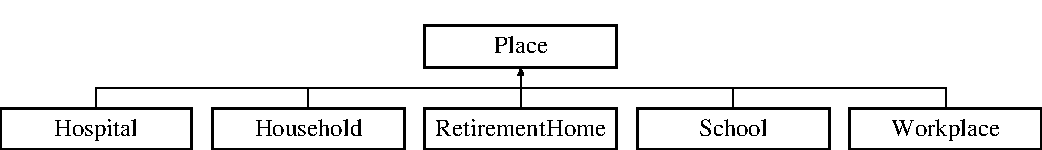
\includegraphics[height=2.000000cm]{classPlace}
\end{center}
\end{figure}
\subsection*{Public Member Functions}
\begin{DoxyCompactItemize}
\item 
\hyperlink{classPlace_ad90eb4021d4c3431e062b3425ed3f05c}{Place} ()=default
\begin{DoxyCompactList}\small\item\em Creates a \hyperlink{classPlace}{Place} object with default attributes. \end{DoxyCompactList}\item 
\hyperlink{classPlace_a4a2f79e0414591c81a2161e055a24ec6}{Place} (const int place\+\_\+\+ID, const double xi, const double yi, const double severity\+\_\+cor, const double beta)
\begin{DoxyCompactList}\small\item\em Creates a \hyperlink{classPlace}{Place} object. \end{DoxyCompactList}\item 
virtual void \hyperlink{classPlace_a96444ff0aa08a921598d0afb9c00cec8}{add\+\_\+exposed} (double inf\+\_\+var)
\begin{DoxyCompactList}\small\item\em Include exposed contribution in the sum. \end{DoxyCompactList}\item 
virtual void \hyperlink{classPlace_a5216539c8589d41aad430513740fa15c}{add\+\_\+symptomatic} (double inf\+\_\+var)
\begin{DoxyCompactList}\small\item\em Include symptomatic contribution in the sum. \end{DoxyCompactList}\item 
virtual void \hyperlink{classPlace_aeb4c561e8bc4e1ae7186baed6ef1aa47}{compute\+\_\+infected\+\_\+contribution} ()
\begin{DoxyCompactList}\small\item\em Calculates and stores fraction of infected agents if any. \end{DoxyCompactList}\item 
virtual void \hyperlink{classPlace_abc1e560ef8aaaad565ccceb9540e5bd8}{reset\+\_\+contributions} ()
\begin{DoxyCompactList}\small\item\em Reset the lambda sum of a place after transmission step. \end{DoxyCompactList}\item 
void \hyperlink{classPlace_a59594ed1acf114ba3a123bd99d874b65}{change\+\_\+transmission\+\_\+rate} (const double new\+\_\+beta)
\item 
int \hyperlink{classPlace_aec0a7e93c669c5e1f72435e2f9052011}{get\+\_\+\+ID} () const
\begin{DoxyCompactList}\small\item\em Return place ID. \end{DoxyCompactList}\item 
virtual std\+::vector$<$ int $>$ \hyperlink{classPlace_a2f6dbc1e8937c6563b04bbf7dde7e00f}{get\+\_\+agent\+\_\+\+I\+Ds} () const
\begin{DoxyCompactList}\small\item\em Return I\+Ds of agents registered in this place. \end{DoxyCompactList}\item 
int \hyperlink{classPlace_a0f1e45a13137205dd65f6e33a0a110a6}{get\+\_\+total\+\_\+infected} () const
\begin{DoxyCompactList}\small\item\em Return total number of infected agents. \end{DoxyCompactList}\item 
double \hyperlink{classPlace_a8a3cc52898c24655efc92f51512a81ce}{get\+\_\+infected\+\_\+contribution} () const
\begin{DoxyCompactList}\small\item\em Return probability contribution of infected agents. \end{DoxyCompactList}\item 
double \hyperlink{classPlace_a024b5b993c0f566135090a4c3336c24c}{get\+\_\+transmission\+\_\+rate} () const
\begin{DoxyCompactList}\small\item\em Transmission rate. \end{DoxyCompactList}\item 
virtual void \hyperlink{classPlace_a9aa7649e0b91c5f61a5f71e9ca808fe1}{print\+\_\+basic} (std\+::ostream \&where) const
\begin{DoxyCompactList}\small\item\em Save information about a \hyperlink{classPlace}{Place} object. \end{DoxyCompactList}\item 
void \hyperlink{classPlace_a2e46294c2fd0e871740e3ddab1095296}{register\+\_\+agent} (const int agent\+\_\+\+ID, const bool is\+\_\+infected)
\begin{DoxyCompactList}\small\item\em Assign agent to a given place indicating if infected. \end{DoxyCompactList}\item 
void \hyperlink{classPlace_a42d0f8ea98161eb76ebebb4f0946b474}{add\+\_\+agent} (const int index)
\begin{DoxyCompactList}\small\item\em Add a new agent to this place. \end{DoxyCompactList}\item 
void \hyperlink{classPlace_aee19c9f59dcaeb02ac3b1e9c8adaa784}{remove\+\_\+agent} (const int index)
\begin{DoxyCompactList}\small\item\em Remove an agent from this place. \end{DoxyCompactList}\item 
virtual \hyperlink{classPlace_a5dedf984133a4a33a95419da61b54157}{$\sim$\+Place} ()=default
\end{DoxyCompactItemize}
\subsection*{Protected Attributes}
\begin{DoxyCompactItemize}
\item 
int \hyperlink{classPlace_ab8c3da5a85a1901600134ee86f8ab903}{ID} = -\/1
\item 
double \hyperlink{classPlace_ac6d563401f03901268237a3eac6c5a91}{x} = 0.\+0
\item 
double \hyperlink{classPlace_aa2db7a2794804023e6e4b239d2583e26}{y} = 0.\+0
\item 
std\+::vector$<$ int $>$ \hyperlink{classPlace_ace9be66da17210f0d5f0900a7eca9583}{agent\+\_\+\+I\+Ds}
\item 
int \hyperlink{classPlace_a203a593f2d9b7f075936b0dab6aa019f}{num\+\_\+tot} = 0
\item 
int \hyperlink{classPlace_aad8ac414868590db5def58a25266ee7d}{num\+\_\+infected} = 0
\item 
double \hyperlink{classPlace_a8eaee99e4b5cb44399fc331e1555409d}{lambda\+\_\+sum} = 0.\+0
\item 
double \hyperlink{classPlace_a404f9bbc4565b6243ff4efd16e614dfd}{lambda\+\_\+tot} = 0.\+0
\item 
double \hyperlink{classPlace_ac69380b31bba06704bf55945187f1d45}{ck} = 0.\+0
\item 
double \hyperlink{classPlace_a458182cfe5057a826792d65000477f12}{beta\+\_\+j} = 0.\+0
\item 
double \hyperlink{classPlace_af6d1304a203b14b9646ae477841d3073}{inf\+\_\+ratio} = 0.\+0
\end{DoxyCompactItemize}


\subsection{Constructor \& Destructor Documentation}
\mbox{\Hypertarget{classPlace_ad90eb4021d4c3431e062b3425ed3f05c}\label{classPlace_ad90eb4021d4c3431e062b3425ed3f05c}} 
\index{Place@{Place}!Place@{Place}}
\index{Place@{Place}!Place@{Place}}
\subsubsection{\texorpdfstring{Place()}{Place()}\hspace{0.1cm}{\footnotesize\ttfamily [1/2]}}
{\footnotesize\ttfamily Place\+::\+Place (\begin{DoxyParamCaption}{ }\end{DoxyParamCaption})\hspace{0.3cm}{\ttfamily [default]}}



Creates a \hyperlink{classPlace}{Place} object with default attributes. 

\mbox{\Hypertarget{classPlace_a4a2f79e0414591c81a2161e055a24ec6}\label{classPlace_a4a2f79e0414591c81a2161e055a24ec6}} 
\index{Place@{Place}!Place@{Place}}
\index{Place@{Place}!Place@{Place}}
\subsubsection{\texorpdfstring{Place()}{Place()}\hspace{0.1cm}{\footnotesize\ttfamily [2/2]}}
{\footnotesize\ttfamily Place\+::\+Place (\begin{DoxyParamCaption}\item[{const int}]{place\+\_\+\+ID,  }\item[{const double}]{xi,  }\item[{const double}]{yi,  }\item[{const double}]{severity\+\_\+cor,  }\item[{const double}]{beta }\end{DoxyParamCaption})\hspace{0.3cm}{\ttfamily [inline]}}



Creates a \hyperlink{classPlace}{Place} object. 

\hyperlink{classPlace}{Place} with custom ID, location, and infection parameters during creation of agents 
\begin{DoxyParams}{Parameters}
{\em place\+\_\+\+ID} & -\/ ID of the place \\
\hline
{\em xi} & -\/ x coordinate of the place \\
\hline
{\em yi} & -\/ y coordinate of the place \\
\hline
{\em severity\+\_\+cor} & -\/ severity correction for symptomatic \\
\hline
{\em beta} & -\/ infection transmission rate, 1/time \\
\hline
\end{DoxyParams}
\mbox{\Hypertarget{classPlace_a5dedf984133a4a33a95419da61b54157}\label{classPlace_a5dedf984133a4a33a95419da61b54157}} 
\index{Place@{Place}!````~Place@{$\sim$\+Place}}
\index{````~Place@{$\sim$\+Place}!Place@{Place}}
\subsubsection{\texorpdfstring{$\sim$\+Place()}{~Place()}}
{\footnotesize\ttfamily virtual Place\+::$\sim$\+Place (\begin{DoxyParamCaption}{ }\end{DoxyParamCaption})\hspace{0.3cm}{\ttfamily [virtual]}, {\ttfamily [default]}}



\subsection{Member Function Documentation}
\mbox{\Hypertarget{classPlace_a42d0f8ea98161eb76ebebb4f0946b474}\label{classPlace_a42d0f8ea98161eb76ebebb4f0946b474}} 
\index{Place@{Place}!add\+\_\+agent@{add\+\_\+agent}}
\index{add\+\_\+agent@{add\+\_\+agent}!Place@{Place}}
\subsubsection{\texorpdfstring{add\+\_\+agent()}{add\_agent()}}
{\footnotesize\ttfamily void Place\+::add\+\_\+agent (\begin{DoxyParamCaption}\item[{const int}]{index }\end{DoxyParamCaption})\hspace{0.3cm}{\ttfamily [inline]}}



Add a new agent to this place. 


\begin{DoxyParams}{Parameters}
{\em index} & -\/ agent ID (starts with 1) \\
\hline
\end{DoxyParams}
\mbox{\Hypertarget{classPlace_a96444ff0aa08a921598d0afb9c00cec8}\label{classPlace_a96444ff0aa08a921598d0afb9c00cec8}} 
\index{Place@{Place}!add\+\_\+exposed@{add\+\_\+exposed}}
\index{add\+\_\+exposed@{add\+\_\+exposed}!Place@{Place}}
\subsubsection{\texorpdfstring{add\+\_\+exposed()}{add\_exposed()}}
{\footnotesize\ttfamily virtual void Place\+::add\+\_\+exposed (\begin{DoxyParamCaption}\item[{double}]{inf\+\_\+var }\end{DoxyParamCaption})\hspace{0.3cm}{\ttfamily [inline]}, {\ttfamily [virtual]}}



Include exposed contribution in the sum. 


\begin{DoxyParams}{Parameters}
{\em inf\+\_\+var} & -\/ agent infectiousness variability factor \\
\hline
\end{DoxyParams}


Reimplemented in \hyperlink{classHospital_a55c2f778b4aeb0f775bb1b45c147c7b8}{Hospital}.

\mbox{\Hypertarget{classPlace_a5216539c8589d41aad430513740fa15c}\label{classPlace_a5216539c8589d41aad430513740fa15c}} 
\index{Place@{Place}!add\+\_\+symptomatic@{add\+\_\+symptomatic}}
\index{add\+\_\+symptomatic@{add\+\_\+symptomatic}!Place@{Place}}
\subsubsection{\texorpdfstring{add\+\_\+symptomatic()}{add\_symptomatic()}}
{\footnotesize\ttfamily virtual void Place\+::add\+\_\+symptomatic (\begin{DoxyParamCaption}\item[{double}]{inf\+\_\+var }\end{DoxyParamCaption})\hspace{0.3cm}{\ttfamily [inline]}, {\ttfamily [virtual]}}



Include symptomatic contribution in the sum. 


\begin{DoxyParams}{Parameters}
{\em inf\+\_\+var} & -\/ agent infectiousness variability factor \\
\hline
\end{DoxyParams}


Reimplemented in \hyperlink{classWorkplace_a48ef6cf8af0753240063ea8c00f4cc63}{Workplace}.

\mbox{\Hypertarget{classPlace_a59594ed1acf114ba3a123bd99d874b65}\label{classPlace_a59594ed1acf114ba3a123bd99d874b65}} 
\index{Place@{Place}!change\+\_\+transmission\+\_\+rate@{change\+\_\+transmission\+\_\+rate}}
\index{change\+\_\+transmission\+\_\+rate@{change\+\_\+transmission\+\_\+rate}!Place@{Place}}
\subsubsection{\texorpdfstring{change\+\_\+transmission\+\_\+rate()}{change\_transmission\_rate()}}
{\footnotesize\ttfamily void Place\+::change\+\_\+transmission\+\_\+rate (\begin{DoxyParamCaption}\item[{const double}]{new\+\_\+beta }\end{DoxyParamCaption})\hspace{0.3cm}{\ttfamily [inline]}}

\mbox{\Hypertarget{classPlace_aeb4c561e8bc4e1ae7186baed6ef1aa47}\label{classPlace_aeb4c561e8bc4e1ae7186baed6ef1aa47}} 
\index{Place@{Place}!compute\+\_\+infected\+\_\+contribution@{compute\+\_\+infected\+\_\+contribution}}
\index{compute\+\_\+infected\+\_\+contribution@{compute\+\_\+infected\+\_\+contribution}!Place@{Place}}
\subsubsection{\texorpdfstring{compute\+\_\+infected\+\_\+contribution()}{compute\_infected\_contribution()}}
{\footnotesize\ttfamily void Place\+::compute\+\_\+infected\+\_\+contribution (\begin{DoxyParamCaption}{ }\end{DoxyParamCaption})\hspace{0.3cm}{\ttfamily [virtual]}}



Calculates and stores fraction of infected agents if any. 



Reimplemented in \hyperlink{classHospital_ad87fc4a53e50a35489c9024892a7c9d6}{Hospital}, and \hyperlink{classHousehold_ae063737d06a7a50aa9b780d7066c1c88}{Household}.

\mbox{\Hypertarget{classPlace_a2f6dbc1e8937c6563b04bbf7dde7e00f}\label{classPlace_a2f6dbc1e8937c6563b04bbf7dde7e00f}} 
\index{Place@{Place}!get\+\_\+agent\+\_\+\+I\+Ds@{get\+\_\+agent\+\_\+\+I\+Ds}}
\index{get\+\_\+agent\+\_\+\+I\+Ds@{get\+\_\+agent\+\_\+\+I\+Ds}!Place@{Place}}
\subsubsection{\texorpdfstring{get\+\_\+agent\+\_\+\+I\+Ds()}{get\_agent\_IDs()}}
{\footnotesize\ttfamily virtual std\+::vector$<$int$>$ Place\+::get\+\_\+agent\+\_\+\+I\+Ds (\begin{DoxyParamCaption}{ }\end{DoxyParamCaption}) const\hspace{0.3cm}{\ttfamily [inline]}, {\ttfamily [virtual]}}



Return I\+Ds of agents registered in this place. 

\mbox{\Hypertarget{classPlace_aec0a7e93c669c5e1f72435e2f9052011}\label{classPlace_aec0a7e93c669c5e1f72435e2f9052011}} 
\index{Place@{Place}!get\+\_\+\+ID@{get\+\_\+\+ID}}
\index{get\+\_\+\+ID@{get\+\_\+\+ID}!Place@{Place}}
\subsubsection{\texorpdfstring{get\+\_\+\+I\+D()}{get\_ID()}}
{\footnotesize\ttfamily int Place\+::get\+\_\+\+ID (\begin{DoxyParamCaption}{ }\end{DoxyParamCaption}) const\hspace{0.3cm}{\ttfamily [inline]}}



Return place ID. 

\mbox{\Hypertarget{classPlace_a8a3cc52898c24655efc92f51512a81ce}\label{classPlace_a8a3cc52898c24655efc92f51512a81ce}} 
\index{Place@{Place}!get\+\_\+infected\+\_\+contribution@{get\+\_\+infected\+\_\+contribution}}
\index{get\+\_\+infected\+\_\+contribution@{get\+\_\+infected\+\_\+contribution}!Place@{Place}}
\subsubsection{\texorpdfstring{get\+\_\+infected\+\_\+contribution()}{get\_infected\_contribution()}}
{\footnotesize\ttfamily double Place\+::get\+\_\+infected\+\_\+contribution (\begin{DoxyParamCaption}{ }\end{DoxyParamCaption}) const\hspace{0.3cm}{\ttfamily [inline]}}



Return probability contribution of infected agents. 

\mbox{\Hypertarget{classPlace_a0f1e45a13137205dd65f6e33a0a110a6}\label{classPlace_a0f1e45a13137205dd65f6e33a0a110a6}} 
\index{Place@{Place}!get\+\_\+total\+\_\+infected@{get\+\_\+total\+\_\+infected}}
\index{get\+\_\+total\+\_\+infected@{get\+\_\+total\+\_\+infected}!Place@{Place}}
\subsubsection{\texorpdfstring{get\+\_\+total\+\_\+infected()}{get\_total\_infected()}}
{\footnotesize\ttfamily int Place\+::get\+\_\+total\+\_\+infected (\begin{DoxyParamCaption}{ }\end{DoxyParamCaption}) const\hspace{0.3cm}{\ttfamily [inline]}}



Return total number of infected agents. 

\mbox{\Hypertarget{classPlace_a024b5b993c0f566135090a4c3336c24c}\label{classPlace_a024b5b993c0f566135090a4c3336c24c}} 
\index{Place@{Place}!get\+\_\+transmission\+\_\+rate@{get\+\_\+transmission\+\_\+rate}}
\index{get\+\_\+transmission\+\_\+rate@{get\+\_\+transmission\+\_\+rate}!Place@{Place}}
\subsubsection{\texorpdfstring{get\+\_\+transmission\+\_\+rate()}{get\_transmission\_rate()}}
{\footnotesize\ttfamily double Place\+::get\+\_\+transmission\+\_\+rate (\begin{DoxyParamCaption}{ }\end{DoxyParamCaption}) const\hspace{0.3cm}{\ttfamily [inline]}}



Transmission rate. 

\mbox{\Hypertarget{classPlace_a9aa7649e0b91c5f61a5f71e9ca808fe1}\label{classPlace_a9aa7649e0b91c5f61a5f71e9ca808fe1}} 
\index{Place@{Place}!print\+\_\+basic@{print\+\_\+basic}}
\index{print\+\_\+basic@{print\+\_\+basic}!Place@{Place}}
\subsubsection{\texorpdfstring{print\+\_\+basic()}{print\_basic()}}
{\footnotesize\ttfamily void Place\+::print\+\_\+basic (\begin{DoxyParamCaption}\item[{std\+::ostream \&}]{where }\end{DoxyParamCaption}) const\hspace{0.3cm}{\ttfamily [virtual]}}



Save information about a \hyperlink{classPlace}{Place} object. 

Saves to a file, everything but detailed agent information; order is ID $\vert$ x $\vert$ y $\vert$ number of agents $\vert$ number of infected agents Delimiter is a space. 
\begin{DoxyParams}{Parameters}
{\em where} & -\/ output stream \\
\hline
\end{DoxyParams}


Reimplemented in \hyperlink{classHospital_a3a1963886a9974663c2a3e82817f1a2b}{Hospital}, \hyperlink{classSchool_ade1610f7c072eb041f6d8b0e157e1cc8}{School}, \hyperlink{classRetirementHome_aafab41675600b03fdffcf11db1a07ec7}{Retirement\+Home}, \hyperlink{classWorkplace_af4fcc642e32e174bab45def56b7c6f05}{Workplace}, and \hyperlink{classHousehold_a9bf27cca25dea519945c8740b9793ff6}{Household}.

\mbox{\Hypertarget{classPlace_a2e46294c2fd0e871740e3ddab1095296}\label{classPlace_a2e46294c2fd0e871740e3ddab1095296}} 
\index{Place@{Place}!register\+\_\+agent@{register\+\_\+agent}}
\index{register\+\_\+agent@{register\+\_\+agent}!Place@{Place}}
\subsubsection{\texorpdfstring{register\+\_\+agent()}{register\_agent()}}
{\footnotesize\ttfamily void Place\+::register\+\_\+agent (\begin{DoxyParamCaption}\item[{const int}]{agent\+\_\+\+ID,  }\item[{const bool}]{is\+\_\+infected }\end{DoxyParamCaption})}



Assign agent to a given place indicating if infected. 


\begin{DoxyParams}{Parameters}
{\em agent\+\_\+\+ID} & -\/ global ID of the agent \\
\hline
{\em is\+\_\+infected} & -\/ true if agent is infected \\
\hline
\end{DoxyParams}
\mbox{\Hypertarget{classPlace_aee19c9f59dcaeb02ac3b1e9c8adaa784}\label{classPlace_aee19c9f59dcaeb02ac3b1e9c8adaa784}} 
\index{Place@{Place}!remove\+\_\+agent@{remove\+\_\+agent}}
\index{remove\+\_\+agent@{remove\+\_\+agent}!Place@{Place}}
\subsubsection{\texorpdfstring{remove\+\_\+agent()}{remove\_agent()}}
{\footnotesize\ttfamily void Place\+::remove\+\_\+agent (\begin{DoxyParamCaption}\item[{const int}]{index }\end{DoxyParamCaption})}



Remove an agent from this place. 


\begin{DoxyParams}{Parameters}
{\em index} & -\/ agent ID (starts with 1) \\
\hline
\end{DoxyParams}
\mbox{\Hypertarget{classPlace_abc1e560ef8aaaad565ccceb9540e5bd8}\label{classPlace_abc1e560ef8aaaad565ccceb9540e5bd8}} 
\index{Place@{Place}!reset\+\_\+contributions@{reset\+\_\+contributions}}
\index{reset\+\_\+contributions@{reset\+\_\+contributions}!Place@{Place}}
\subsubsection{\texorpdfstring{reset\+\_\+contributions()}{reset\_contributions()}}
{\footnotesize\ttfamily virtual void Place\+::reset\+\_\+contributions (\begin{DoxyParamCaption}{ }\end{DoxyParamCaption})\hspace{0.3cm}{\ttfamily [inline]}, {\ttfamily [virtual]}}



Reset the lambda sum of a place after transmission step. 



Reimplemented in \hyperlink{classHospital_a928d185dde78d0bce3034b7a138b472d}{Hospital}.



\subsection{Member Data Documentation}
\mbox{\Hypertarget{classPlace_ace9be66da17210f0d5f0900a7eca9583}\label{classPlace_ace9be66da17210f0d5f0900a7eca9583}} 
\index{Place@{Place}!agent\+\_\+\+I\+Ds@{agent\+\_\+\+I\+Ds}}
\index{agent\+\_\+\+I\+Ds@{agent\+\_\+\+I\+Ds}!Place@{Place}}
\subsubsection{\texorpdfstring{agent\+\_\+\+I\+Ds}{agent\_IDs}}
{\footnotesize\ttfamily std\+::vector$<$int$>$ Place\+::agent\+\_\+\+I\+Ds\hspace{0.3cm}{\ttfamily [protected]}}

\mbox{\Hypertarget{classPlace_a458182cfe5057a826792d65000477f12}\label{classPlace_a458182cfe5057a826792d65000477f12}} 
\index{Place@{Place}!beta\+\_\+j@{beta\+\_\+j}}
\index{beta\+\_\+j@{beta\+\_\+j}!Place@{Place}}
\subsubsection{\texorpdfstring{beta\+\_\+j}{beta\_j}}
{\footnotesize\ttfamily double Place\+::beta\+\_\+j = 0.\+0\hspace{0.3cm}{\ttfamily [protected]}}

\mbox{\Hypertarget{classPlace_ac69380b31bba06704bf55945187f1d45}\label{classPlace_ac69380b31bba06704bf55945187f1d45}} 
\index{Place@{Place}!ck@{ck}}
\index{ck@{ck}!Place@{Place}}
\subsubsection{\texorpdfstring{ck}{ck}}
{\footnotesize\ttfamily double Place\+::ck = 0.\+0\hspace{0.3cm}{\ttfamily [protected]}}

\mbox{\Hypertarget{classPlace_ab8c3da5a85a1901600134ee86f8ab903}\label{classPlace_ab8c3da5a85a1901600134ee86f8ab903}} 
\index{Place@{Place}!ID@{ID}}
\index{ID@{ID}!Place@{Place}}
\subsubsection{\texorpdfstring{ID}{ID}}
{\footnotesize\ttfamily int Place\+::\+ID = -\/1\hspace{0.3cm}{\ttfamily [protected]}}

\mbox{\Hypertarget{classPlace_af6d1304a203b14b9646ae477841d3073}\label{classPlace_af6d1304a203b14b9646ae477841d3073}} 
\index{Place@{Place}!inf\+\_\+ratio@{inf\+\_\+ratio}}
\index{inf\+\_\+ratio@{inf\+\_\+ratio}!Place@{Place}}
\subsubsection{\texorpdfstring{inf\+\_\+ratio}{inf\_ratio}}
{\footnotesize\ttfamily double Place\+::inf\+\_\+ratio = 0.\+0\hspace{0.3cm}{\ttfamily [protected]}}

\mbox{\Hypertarget{classPlace_a8eaee99e4b5cb44399fc331e1555409d}\label{classPlace_a8eaee99e4b5cb44399fc331e1555409d}} 
\index{Place@{Place}!lambda\+\_\+sum@{lambda\+\_\+sum}}
\index{lambda\+\_\+sum@{lambda\+\_\+sum}!Place@{Place}}
\subsubsection{\texorpdfstring{lambda\+\_\+sum}{lambda\_sum}}
{\footnotesize\ttfamily double Place\+::lambda\+\_\+sum = 0.\+0\hspace{0.3cm}{\ttfamily [protected]}}

\mbox{\Hypertarget{classPlace_a404f9bbc4565b6243ff4efd16e614dfd}\label{classPlace_a404f9bbc4565b6243ff4efd16e614dfd}} 
\index{Place@{Place}!lambda\+\_\+tot@{lambda\+\_\+tot}}
\index{lambda\+\_\+tot@{lambda\+\_\+tot}!Place@{Place}}
\subsubsection{\texorpdfstring{lambda\+\_\+tot}{lambda\_tot}}
{\footnotesize\ttfamily double Place\+::lambda\+\_\+tot = 0.\+0\hspace{0.3cm}{\ttfamily [protected]}}

\mbox{\Hypertarget{classPlace_aad8ac414868590db5def58a25266ee7d}\label{classPlace_aad8ac414868590db5def58a25266ee7d}} 
\index{Place@{Place}!num\+\_\+infected@{num\+\_\+infected}}
\index{num\+\_\+infected@{num\+\_\+infected}!Place@{Place}}
\subsubsection{\texorpdfstring{num\+\_\+infected}{num\_infected}}
{\footnotesize\ttfamily int Place\+::num\+\_\+infected = 0\hspace{0.3cm}{\ttfamily [protected]}}

\mbox{\Hypertarget{classPlace_a203a593f2d9b7f075936b0dab6aa019f}\label{classPlace_a203a593f2d9b7f075936b0dab6aa019f}} 
\index{Place@{Place}!num\+\_\+tot@{num\+\_\+tot}}
\index{num\+\_\+tot@{num\+\_\+tot}!Place@{Place}}
\subsubsection{\texorpdfstring{num\+\_\+tot}{num\_tot}}
{\footnotesize\ttfamily int Place\+::num\+\_\+tot = 0\hspace{0.3cm}{\ttfamily [protected]}}

\mbox{\Hypertarget{classPlace_ac6d563401f03901268237a3eac6c5a91}\label{classPlace_ac6d563401f03901268237a3eac6c5a91}} 
\index{Place@{Place}!x@{x}}
\index{x@{x}!Place@{Place}}
\subsubsection{\texorpdfstring{x}{x}}
{\footnotesize\ttfamily double Place\+::x = 0.\+0\hspace{0.3cm}{\ttfamily [protected]}}

\mbox{\Hypertarget{classPlace_aa2db7a2794804023e6e4b239d2583e26}\label{classPlace_aa2db7a2794804023e6e4b239d2583e26}} 
\index{Place@{Place}!y@{y}}
\index{y@{y}!Place@{Place}}
\subsubsection{\texorpdfstring{y}{y}}
{\footnotesize\ttfamily double Place\+::y = 0.\+0\hspace{0.3cm}{\ttfamily [protected]}}



The documentation for this class was generated from the following files\+:\begin{DoxyCompactItemize}
\item 
include/places/\hyperlink{place_8h}{place.\+h}\item 
src/places/\hyperlink{place_8cpp}{place.\+cpp}\end{DoxyCompactItemize}

\hypertarget{classRegularStatesManager}{}\section{Regular\+States\+Manager Class Reference}
\label{classRegularStatesManager}\index{Regular\+States\+Manager@{Regular\+States\+Manager}}


{\ttfamily \#include $<$regular\+\_\+states\+\_\+manager.\+h$>$}

\subsection*{Public Member Functions}
\begin{DoxyCompactItemize}
\item 
\hyperlink{classRegularStatesManager_a05c6533bf5e460afef3e89d75413a510}{Regular\+States\+Manager} ()=default
\item 
void \hyperlink{classRegularStatesManager_a123ac58f69fd27b51fbb6068755b61aa}{set\+\_\+susceptible\+\_\+to\+\_\+exposed} (\hyperlink{classAgent}{Agent} \&agent)
\begin{DoxyCompactList}\small\item\em Set all states for transition from susceptible to exposed. \end{DoxyCompactList}\item 
void \hyperlink{classRegularStatesManager_a3a1ad21ed23f705b9d35ab1b5ed74d06}{set\+\_\+susceptible\+\_\+to\+\_\+exposed\+\_\+never\+\_\+symptomatic} (\hyperlink{classAgent}{Agent} \&agent)
\begin{DoxyCompactList}\small\item\em Set all states for transition from susceptible to exposed that will never become symptomatic. \end{DoxyCompactList}\item 
void \hyperlink{classRegularStatesManager_a1378bb9ee86f261d5bf7c66c7798e1b4}{set\+\_\+exposed\+\_\+never\+\_\+symptomatic\+\_\+to\+\_\+removed} (\hyperlink{classAgent}{Agent} \&agent)
\begin{DoxyCompactList}\small\item\em Set exposed that never developed symptoms to removed. \end{DoxyCompactList}\item 
void \hyperlink{classRegularStatesManager_a943fe599632b05929f56353471423955}{set\+\_\+exposed\+\_\+to\+\_\+symptomatic} (\hyperlink{classAgent}{Agent} \&agent)
\begin{DoxyCompactList}\small\item\em Set all states for transition from exposed to general symptomatic. \end{DoxyCompactList}\item 
void \hyperlink{classRegularStatesManager_a7ebe37dca3740a25fa0682eb471be976}{set\+\_\+dying\+\_\+symptomatic} (\hyperlink{classAgent}{Agent} \&agent)
\begin{DoxyCompactList}\small\item\em Set all states relevant to agent that will die. \end{DoxyCompactList}\item 
void \hyperlink{classRegularStatesManager_a2c1745d45af0aeaf11b5b6718ab8c2d1}{set\+\_\+recovering\+\_\+symptomatic} (\hyperlink{classAgent}{Agent} \&agent)
\begin{DoxyCompactList}\small\item\em Set all states relevant to agent that will recover. \end{DoxyCompactList}\item 
void \hyperlink{classRegularStatesManager_adfe4e02af0388ceb0adba80867079ca7}{set\+\_\+waiting\+\_\+for\+\_\+test\+\_\+in\+\_\+hospital} (\hyperlink{classAgent}{Agent} \&agent)
\begin{DoxyCompactList}\small\item\em Set testing in hospital, initial state. \end{DoxyCompactList}\item 
void \hyperlink{classRegularStatesManager_aac23ea794e2797e61648e3826a9f8eac}{set\+\_\+exposed\+\_\+waiting\+\_\+for\+\_\+test\+\_\+in\+\_\+hospital} (\hyperlink{classAgent}{Agent} \&agent)
\begin{DoxyCompactList}\small\item\em Set testing in hospital, initial state. \end{DoxyCompactList}\item 
void \hyperlink{classRegularStatesManager_abbb119bf6ac68db9594fda91be9b2ee4}{set\+\_\+waiting\+\_\+for\+\_\+test\+\_\+in\+\_\+car} (\hyperlink{classAgent}{Agent} \&agent)
\begin{DoxyCompactList}\small\item\em Set testing in a car, initial state. \end{DoxyCompactList}\item 
void \hyperlink{classRegularStatesManager_a89a7a051bd5b196dc8db2b1343f62f04}{set\+\_\+exposed\+\_\+waiting\+\_\+for\+\_\+test\+\_\+in\+\_\+car} (\hyperlink{classAgent}{Agent} \&agent)
\begin{DoxyCompactList}\small\item\em Set testing in a car, initial state. \end{DoxyCompactList}\item 
void \hyperlink{classRegularStatesManager_a65490a9d9e523ed87acb5b36444ccbba}{set\+\_\+tested\+\_\+to\+\_\+awaiting\+\_\+results} (\hyperlink{classAgent}{Agent} \&agent)
\begin{DoxyCompactList}\small\item\em Set all states for just tested. \end{DoxyCompactList}\item 
void \hyperlink{classRegularStatesManager_a82b160b267cc70b5c599119fd278936d}{set\+\_\+tested\+\_\+false\+\_\+negative} (\hyperlink{classAgent}{Agent} \&agent)
\begin{DoxyCompactList}\small\item\em Set all states for transition from tested to false negative. \end{DoxyCompactList}\item 
void \hyperlink{classRegularStatesManager_af04422e175919ff93d09f19832fc122c}{set\+\_\+icu\+\_\+dying} (\hyperlink{classAgent}{Agent} \&agent)
\begin{DoxyCompactList}\small\item\em States for hospitalized, I\+CU -\/ dying. \end{DoxyCompactList}\item 
void \hyperlink{classRegularStatesManager_a34094d08eb2378f7e02d73da4599fab7}{set\+\_\+icu\+\_\+recovering} (\hyperlink{classAgent}{Agent} \&agent)
\begin{DoxyCompactList}\small\item\em States for hospitalized, I\+CU -\/ recovering. \end{DoxyCompactList}\item 
void \hyperlink{classRegularStatesManager_aba141d47c1bf1e7de90a5d12d6cbcb65}{set\+\_\+hospitalized} (\hyperlink{classAgent}{Agent} \&agent)
\begin{DoxyCompactList}\small\item\em States for hospitalized. \end{DoxyCompactList}\item 
void \hyperlink{classRegularStatesManager_a1be9c0452ba637272cf12ceeec82eda7}{set\+\_\+home\+\_\+isolation} (\hyperlink{classAgent}{Agent} \&agent)
\begin{DoxyCompactList}\small\item\em States for isolated at home. \end{DoxyCompactList}\item 
void \hyperlink{classRegularStatesManager_a3f6d863ccc2712cc6b742369e8903d3f}{set\+\_\+any\+\_\+to\+\_\+removed} (\hyperlink{classAgent}{Agent} \&agent)
\begin{DoxyCompactList}\small\item\em Set all removed related states. \end{DoxyCompactList}\item 
void \hyperlink{classRegularStatesManager_a061efc051ba2c64a02a2ce66d915a610}{set\+\_\+former\+\_\+flu} (\hyperlink{classAgent}{Agent} \&agent)
\begin{DoxyCompactList}\small\item\em Reset all flu related flags to false. \end{DoxyCompactList}\item 
void \hyperlink{classRegularStatesManager_a7bdff7e59ae0d521f32ec1a33d7c2c41}{set\+\_\+tested\+\_\+false\+\_\+positive} (\hyperlink{classAgent}{Agent} \&agent)
\begin{DoxyCompactList}\small\item\em States for false positive, isolated at home. \end{DoxyCompactList}\item 
void \hyperlink{classRegularStatesManager_af336981bd4dfe51eaca43262b89632d3}{set\+\_\+tested\+\_\+negative} (\hyperlink{classAgent}{Agent} \&agent)
\begin{DoxyCompactList}\small\item\em States for negative. \end{DoxyCompactList}\item 
void \hyperlink{classRegularStatesManager_ab225ce7069cd51e2c451ac8fbd28c3e3}{reset\+\_\+returning\+\_\+flu} (\hyperlink{classAgent}{Agent} \&agent)
\begin{DoxyCompactList}\small\item\em Reset flags for flu that is back to susceptible from IH. \end{DoxyCompactList}\end{DoxyCompactItemize}


\subsection{Constructor \& Destructor Documentation}
\mbox{\Hypertarget{classRegularStatesManager_a05c6533bf5e460afef3e89d75413a510}\label{classRegularStatesManager_a05c6533bf5e460afef3e89d75413a510}} 
\index{Regular\+States\+Manager@{Regular\+States\+Manager}!Regular\+States\+Manager@{Regular\+States\+Manager}}
\index{Regular\+States\+Manager@{Regular\+States\+Manager}!Regular\+States\+Manager@{Regular\+States\+Manager}}
\subsubsection{\texorpdfstring{Regular\+States\+Manager()}{RegularStatesManager()}}
{\footnotesize\ttfamily Regular\+States\+Manager\+::\+Regular\+States\+Manager (\begin{DoxyParamCaption}{ }\end{DoxyParamCaption})\hspace{0.3cm}{\ttfamily [default]}}



\subsection{Member Function Documentation}
\mbox{\Hypertarget{classRegularStatesManager_ab225ce7069cd51e2c451ac8fbd28c3e3}\label{classRegularStatesManager_ab225ce7069cd51e2c451ac8fbd28c3e3}} 
\index{Regular\+States\+Manager@{Regular\+States\+Manager}!reset\+\_\+returning\+\_\+flu@{reset\+\_\+returning\+\_\+flu}}
\index{reset\+\_\+returning\+\_\+flu@{reset\+\_\+returning\+\_\+flu}!Regular\+States\+Manager@{Regular\+States\+Manager}}
\subsubsection{\texorpdfstring{reset\+\_\+returning\+\_\+flu()}{reset\_returning\_flu()}}
{\footnotesize\ttfamily void Regular\+States\+Manager\+::reset\+\_\+returning\+\_\+flu (\begin{DoxyParamCaption}\item[{\hyperlink{classAgent}{Agent} \&}]{agent }\end{DoxyParamCaption})}



Reset flags for flu that is back to susceptible from IH. 

\mbox{\Hypertarget{classRegularStatesManager_a3f6d863ccc2712cc6b742369e8903d3f}\label{classRegularStatesManager_a3f6d863ccc2712cc6b742369e8903d3f}} 
\index{Regular\+States\+Manager@{Regular\+States\+Manager}!set\+\_\+any\+\_\+to\+\_\+removed@{set\+\_\+any\+\_\+to\+\_\+removed}}
\index{set\+\_\+any\+\_\+to\+\_\+removed@{set\+\_\+any\+\_\+to\+\_\+removed}!Regular\+States\+Manager@{Regular\+States\+Manager}}
\subsubsection{\texorpdfstring{set\+\_\+any\+\_\+to\+\_\+removed()}{set\_any\_to\_removed()}}
{\footnotesize\ttfamily void Regular\+States\+Manager\+::set\+\_\+any\+\_\+to\+\_\+removed (\begin{DoxyParamCaption}\item[{\hyperlink{classAgent}{Agent} \&}]{agent }\end{DoxyParamCaption})}



Set all removed related states. 

\mbox{\Hypertarget{classRegularStatesManager_a7ebe37dca3740a25fa0682eb471be976}\label{classRegularStatesManager_a7ebe37dca3740a25fa0682eb471be976}} 
\index{Regular\+States\+Manager@{Regular\+States\+Manager}!set\+\_\+dying\+\_\+symptomatic@{set\+\_\+dying\+\_\+symptomatic}}
\index{set\+\_\+dying\+\_\+symptomatic@{set\+\_\+dying\+\_\+symptomatic}!Regular\+States\+Manager@{Regular\+States\+Manager}}
\subsubsection{\texorpdfstring{set\+\_\+dying\+\_\+symptomatic()}{set\_dying\_symptomatic()}}
{\footnotesize\ttfamily void Regular\+States\+Manager\+::set\+\_\+dying\+\_\+symptomatic (\begin{DoxyParamCaption}\item[{\hyperlink{classAgent}{Agent} \&}]{agent }\end{DoxyParamCaption})}



Set all states relevant to agent that will die. 

\mbox{\Hypertarget{classRegularStatesManager_a1378bb9ee86f261d5bf7c66c7798e1b4}\label{classRegularStatesManager_a1378bb9ee86f261d5bf7c66c7798e1b4}} 
\index{Regular\+States\+Manager@{Regular\+States\+Manager}!set\+\_\+exposed\+\_\+never\+\_\+symptomatic\+\_\+to\+\_\+removed@{set\+\_\+exposed\+\_\+never\+\_\+symptomatic\+\_\+to\+\_\+removed}}
\index{set\+\_\+exposed\+\_\+never\+\_\+symptomatic\+\_\+to\+\_\+removed@{set\+\_\+exposed\+\_\+never\+\_\+symptomatic\+\_\+to\+\_\+removed}!Regular\+States\+Manager@{Regular\+States\+Manager}}
\subsubsection{\texorpdfstring{set\+\_\+exposed\+\_\+never\+\_\+symptomatic\+\_\+to\+\_\+removed()}{set\_exposed\_never\_symptomatic\_to\_removed()}}
{\footnotesize\ttfamily void Regular\+States\+Manager\+::set\+\_\+exposed\+\_\+never\+\_\+symptomatic\+\_\+to\+\_\+removed (\begin{DoxyParamCaption}\item[{\hyperlink{classAgent}{Agent} \&}]{agent }\end{DoxyParamCaption})}



Set exposed that never developed symptoms to removed. 

\mbox{\Hypertarget{classRegularStatesManager_a943fe599632b05929f56353471423955}\label{classRegularStatesManager_a943fe599632b05929f56353471423955}} 
\index{Regular\+States\+Manager@{Regular\+States\+Manager}!set\+\_\+exposed\+\_\+to\+\_\+symptomatic@{set\+\_\+exposed\+\_\+to\+\_\+symptomatic}}
\index{set\+\_\+exposed\+\_\+to\+\_\+symptomatic@{set\+\_\+exposed\+\_\+to\+\_\+symptomatic}!Regular\+States\+Manager@{Regular\+States\+Manager}}
\subsubsection{\texorpdfstring{set\+\_\+exposed\+\_\+to\+\_\+symptomatic()}{set\_exposed\_to\_symptomatic()}}
{\footnotesize\ttfamily void Regular\+States\+Manager\+::set\+\_\+exposed\+\_\+to\+\_\+symptomatic (\begin{DoxyParamCaption}\item[{\hyperlink{classAgent}{Agent} \&}]{agent }\end{DoxyParamCaption})}



Set all states for transition from exposed to general symptomatic. 

\mbox{\Hypertarget{classRegularStatesManager_a89a7a051bd5b196dc8db2b1343f62f04}\label{classRegularStatesManager_a89a7a051bd5b196dc8db2b1343f62f04}} 
\index{Regular\+States\+Manager@{Regular\+States\+Manager}!set\+\_\+exposed\+\_\+waiting\+\_\+for\+\_\+test\+\_\+in\+\_\+car@{set\+\_\+exposed\+\_\+waiting\+\_\+for\+\_\+test\+\_\+in\+\_\+car}}
\index{set\+\_\+exposed\+\_\+waiting\+\_\+for\+\_\+test\+\_\+in\+\_\+car@{set\+\_\+exposed\+\_\+waiting\+\_\+for\+\_\+test\+\_\+in\+\_\+car}!Regular\+States\+Manager@{Regular\+States\+Manager}}
\subsubsection{\texorpdfstring{set\+\_\+exposed\+\_\+waiting\+\_\+for\+\_\+test\+\_\+in\+\_\+car()}{set\_exposed\_waiting\_for\_test\_in\_car()}}
{\footnotesize\ttfamily void Regular\+States\+Manager\+::set\+\_\+exposed\+\_\+waiting\+\_\+for\+\_\+test\+\_\+in\+\_\+car (\begin{DoxyParamCaption}\item[{\hyperlink{classAgent}{Agent} \&}]{agent }\end{DoxyParamCaption})}



Set testing in a car, initial state. 

\mbox{\Hypertarget{classRegularStatesManager_aac23ea794e2797e61648e3826a9f8eac}\label{classRegularStatesManager_aac23ea794e2797e61648e3826a9f8eac}} 
\index{Regular\+States\+Manager@{Regular\+States\+Manager}!set\+\_\+exposed\+\_\+waiting\+\_\+for\+\_\+test\+\_\+in\+\_\+hospital@{set\+\_\+exposed\+\_\+waiting\+\_\+for\+\_\+test\+\_\+in\+\_\+hospital}}
\index{set\+\_\+exposed\+\_\+waiting\+\_\+for\+\_\+test\+\_\+in\+\_\+hospital@{set\+\_\+exposed\+\_\+waiting\+\_\+for\+\_\+test\+\_\+in\+\_\+hospital}!Regular\+States\+Manager@{Regular\+States\+Manager}}
\subsubsection{\texorpdfstring{set\+\_\+exposed\+\_\+waiting\+\_\+for\+\_\+test\+\_\+in\+\_\+hospital()}{set\_exposed\_waiting\_for\_test\_in\_hospital()}}
{\footnotesize\ttfamily void Regular\+States\+Manager\+::set\+\_\+exposed\+\_\+waiting\+\_\+for\+\_\+test\+\_\+in\+\_\+hospital (\begin{DoxyParamCaption}\item[{\hyperlink{classAgent}{Agent} \&}]{agent }\end{DoxyParamCaption})}



Set testing in hospital, initial state. 

\mbox{\Hypertarget{classRegularStatesManager_a061efc051ba2c64a02a2ce66d915a610}\label{classRegularStatesManager_a061efc051ba2c64a02a2ce66d915a610}} 
\index{Regular\+States\+Manager@{Regular\+States\+Manager}!set\+\_\+former\+\_\+flu@{set\+\_\+former\+\_\+flu}}
\index{set\+\_\+former\+\_\+flu@{set\+\_\+former\+\_\+flu}!Regular\+States\+Manager@{Regular\+States\+Manager}}
\subsubsection{\texorpdfstring{set\+\_\+former\+\_\+flu()}{set\_former\_flu()}}
{\footnotesize\ttfamily void Regular\+States\+Manager\+::set\+\_\+former\+\_\+flu (\begin{DoxyParamCaption}\item[{\hyperlink{classAgent}{Agent} \&}]{agent }\end{DoxyParamCaption})}



Reset all flu related flags to false. 

\mbox{\Hypertarget{classRegularStatesManager_a1be9c0452ba637272cf12ceeec82eda7}\label{classRegularStatesManager_a1be9c0452ba637272cf12ceeec82eda7}} 
\index{Regular\+States\+Manager@{Regular\+States\+Manager}!set\+\_\+home\+\_\+isolation@{set\+\_\+home\+\_\+isolation}}
\index{set\+\_\+home\+\_\+isolation@{set\+\_\+home\+\_\+isolation}!Regular\+States\+Manager@{Regular\+States\+Manager}}
\subsubsection{\texorpdfstring{set\+\_\+home\+\_\+isolation()}{set\_home\_isolation()}}
{\footnotesize\ttfamily void Regular\+States\+Manager\+::set\+\_\+home\+\_\+isolation (\begin{DoxyParamCaption}\item[{\hyperlink{classAgent}{Agent} \&}]{agent }\end{DoxyParamCaption})}



States for isolated at home. 

\mbox{\Hypertarget{classRegularStatesManager_aba141d47c1bf1e7de90a5d12d6cbcb65}\label{classRegularStatesManager_aba141d47c1bf1e7de90a5d12d6cbcb65}} 
\index{Regular\+States\+Manager@{Regular\+States\+Manager}!set\+\_\+hospitalized@{set\+\_\+hospitalized}}
\index{set\+\_\+hospitalized@{set\+\_\+hospitalized}!Regular\+States\+Manager@{Regular\+States\+Manager}}
\subsubsection{\texorpdfstring{set\+\_\+hospitalized()}{set\_hospitalized()}}
{\footnotesize\ttfamily void Regular\+States\+Manager\+::set\+\_\+hospitalized (\begin{DoxyParamCaption}\item[{\hyperlink{classAgent}{Agent} \&}]{agent }\end{DoxyParamCaption})}



States for hospitalized. 

\mbox{\Hypertarget{classRegularStatesManager_af04422e175919ff93d09f19832fc122c}\label{classRegularStatesManager_af04422e175919ff93d09f19832fc122c}} 
\index{Regular\+States\+Manager@{Regular\+States\+Manager}!set\+\_\+icu\+\_\+dying@{set\+\_\+icu\+\_\+dying}}
\index{set\+\_\+icu\+\_\+dying@{set\+\_\+icu\+\_\+dying}!Regular\+States\+Manager@{Regular\+States\+Manager}}
\subsubsection{\texorpdfstring{set\+\_\+icu\+\_\+dying()}{set\_icu\_dying()}}
{\footnotesize\ttfamily void Regular\+States\+Manager\+::set\+\_\+icu\+\_\+dying (\begin{DoxyParamCaption}\item[{\hyperlink{classAgent}{Agent} \&}]{agent }\end{DoxyParamCaption})}



States for hospitalized, I\+CU -\/ dying. 

\mbox{\Hypertarget{classRegularStatesManager_a34094d08eb2378f7e02d73da4599fab7}\label{classRegularStatesManager_a34094d08eb2378f7e02d73da4599fab7}} 
\index{Regular\+States\+Manager@{Regular\+States\+Manager}!set\+\_\+icu\+\_\+recovering@{set\+\_\+icu\+\_\+recovering}}
\index{set\+\_\+icu\+\_\+recovering@{set\+\_\+icu\+\_\+recovering}!Regular\+States\+Manager@{Regular\+States\+Manager}}
\subsubsection{\texorpdfstring{set\+\_\+icu\+\_\+recovering()}{set\_icu\_recovering()}}
{\footnotesize\ttfamily void Regular\+States\+Manager\+::set\+\_\+icu\+\_\+recovering (\begin{DoxyParamCaption}\item[{\hyperlink{classAgent}{Agent} \&}]{agent }\end{DoxyParamCaption})}



States for hospitalized, I\+CU -\/ recovering. 

\mbox{\Hypertarget{classRegularStatesManager_a2c1745d45af0aeaf11b5b6718ab8c2d1}\label{classRegularStatesManager_a2c1745d45af0aeaf11b5b6718ab8c2d1}} 
\index{Regular\+States\+Manager@{Regular\+States\+Manager}!set\+\_\+recovering\+\_\+symptomatic@{set\+\_\+recovering\+\_\+symptomatic}}
\index{set\+\_\+recovering\+\_\+symptomatic@{set\+\_\+recovering\+\_\+symptomatic}!Regular\+States\+Manager@{Regular\+States\+Manager}}
\subsubsection{\texorpdfstring{set\+\_\+recovering\+\_\+symptomatic()}{set\_recovering\_symptomatic()}}
{\footnotesize\ttfamily void Regular\+States\+Manager\+::set\+\_\+recovering\+\_\+symptomatic (\begin{DoxyParamCaption}\item[{\hyperlink{classAgent}{Agent} \&}]{agent }\end{DoxyParamCaption})}



Set all states relevant to agent that will recover. 

\mbox{\Hypertarget{classRegularStatesManager_a123ac58f69fd27b51fbb6068755b61aa}\label{classRegularStatesManager_a123ac58f69fd27b51fbb6068755b61aa}} 
\index{Regular\+States\+Manager@{Regular\+States\+Manager}!set\+\_\+susceptible\+\_\+to\+\_\+exposed@{set\+\_\+susceptible\+\_\+to\+\_\+exposed}}
\index{set\+\_\+susceptible\+\_\+to\+\_\+exposed@{set\+\_\+susceptible\+\_\+to\+\_\+exposed}!Regular\+States\+Manager@{Regular\+States\+Manager}}
\subsubsection{\texorpdfstring{set\+\_\+susceptible\+\_\+to\+\_\+exposed()}{set\_susceptible\_to\_exposed()}}
{\footnotesize\ttfamily void Regular\+States\+Manager\+::set\+\_\+susceptible\+\_\+to\+\_\+exposed (\begin{DoxyParamCaption}\item[{\hyperlink{classAgent}{Agent} \&}]{agent }\end{DoxyParamCaption})}



Set all states for transition from susceptible to exposed. 

\mbox{\Hypertarget{classRegularStatesManager_a3a1ad21ed23f705b9d35ab1b5ed74d06}\label{classRegularStatesManager_a3a1ad21ed23f705b9d35ab1b5ed74d06}} 
\index{Regular\+States\+Manager@{Regular\+States\+Manager}!set\+\_\+susceptible\+\_\+to\+\_\+exposed\+\_\+never\+\_\+symptomatic@{set\+\_\+susceptible\+\_\+to\+\_\+exposed\+\_\+never\+\_\+symptomatic}}
\index{set\+\_\+susceptible\+\_\+to\+\_\+exposed\+\_\+never\+\_\+symptomatic@{set\+\_\+susceptible\+\_\+to\+\_\+exposed\+\_\+never\+\_\+symptomatic}!Regular\+States\+Manager@{Regular\+States\+Manager}}
\subsubsection{\texorpdfstring{set\+\_\+susceptible\+\_\+to\+\_\+exposed\+\_\+never\+\_\+symptomatic()}{set\_susceptible\_to\_exposed\_never\_symptomatic()}}
{\footnotesize\ttfamily void Regular\+States\+Manager\+::set\+\_\+susceptible\+\_\+to\+\_\+exposed\+\_\+never\+\_\+symptomatic (\begin{DoxyParamCaption}\item[{\hyperlink{classAgent}{Agent} \&}]{agent }\end{DoxyParamCaption})}



Set all states for transition from susceptible to exposed that will never become symptomatic. 

\mbox{\Hypertarget{classRegularStatesManager_a82b160b267cc70b5c599119fd278936d}\label{classRegularStatesManager_a82b160b267cc70b5c599119fd278936d}} 
\index{Regular\+States\+Manager@{Regular\+States\+Manager}!set\+\_\+tested\+\_\+false\+\_\+negative@{set\+\_\+tested\+\_\+false\+\_\+negative}}
\index{set\+\_\+tested\+\_\+false\+\_\+negative@{set\+\_\+tested\+\_\+false\+\_\+negative}!Regular\+States\+Manager@{Regular\+States\+Manager}}
\subsubsection{\texorpdfstring{set\+\_\+tested\+\_\+false\+\_\+negative()}{set\_tested\_false\_negative()}}
{\footnotesize\ttfamily void Regular\+States\+Manager\+::set\+\_\+tested\+\_\+false\+\_\+negative (\begin{DoxyParamCaption}\item[{\hyperlink{classAgent}{Agent} \&}]{agent }\end{DoxyParamCaption})}



Set all states for transition from tested to false negative. 

\mbox{\Hypertarget{classRegularStatesManager_a7bdff7e59ae0d521f32ec1a33d7c2c41}\label{classRegularStatesManager_a7bdff7e59ae0d521f32ec1a33d7c2c41}} 
\index{Regular\+States\+Manager@{Regular\+States\+Manager}!set\+\_\+tested\+\_\+false\+\_\+positive@{set\+\_\+tested\+\_\+false\+\_\+positive}}
\index{set\+\_\+tested\+\_\+false\+\_\+positive@{set\+\_\+tested\+\_\+false\+\_\+positive}!Regular\+States\+Manager@{Regular\+States\+Manager}}
\subsubsection{\texorpdfstring{set\+\_\+tested\+\_\+false\+\_\+positive()}{set\_tested\_false\_positive()}}
{\footnotesize\ttfamily void Regular\+States\+Manager\+::set\+\_\+tested\+\_\+false\+\_\+positive (\begin{DoxyParamCaption}\item[{\hyperlink{classAgent}{Agent} \&}]{agent }\end{DoxyParamCaption})}



States for false positive, isolated at home. 

\mbox{\Hypertarget{classRegularStatesManager_af336981bd4dfe51eaca43262b89632d3}\label{classRegularStatesManager_af336981bd4dfe51eaca43262b89632d3}} 
\index{Regular\+States\+Manager@{Regular\+States\+Manager}!set\+\_\+tested\+\_\+negative@{set\+\_\+tested\+\_\+negative}}
\index{set\+\_\+tested\+\_\+negative@{set\+\_\+tested\+\_\+negative}!Regular\+States\+Manager@{Regular\+States\+Manager}}
\subsubsection{\texorpdfstring{set\+\_\+tested\+\_\+negative()}{set\_tested\_negative()}}
{\footnotesize\ttfamily void Regular\+States\+Manager\+::set\+\_\+tested\+\_\+negative (\begin{DoxyParamCaption}\item[{\hyperlink{classAgent}{Agent} \&}]{agent }\end{DoxyParamCaption})}



States for negative. 

\mbox{\Hypertarget{classRegularStatesManager_a65490a9d9e523ed87acb5b36444ccbba}\label{classRegularStatesManager_a65490a9d9e523ed87acb5b36444ccbba}} 
\index{Regular\+States\+Manager@{Regular\+States\+Manager}!set\+\_\+tested\+\_\+to\+\_\+awaiting\+\_\+results@{set\+\_\+tested\+\_\+to\+\_\+awaiting\+\_\+results}}
\index{set\+\_\+tested\+\_\+to\+\_\+awaiting\+\_\+results@{set\+\_\+tested\+\_\+to\+\_\+awaiting\+\_\+results}!Regular\+States\+Manager@{Regular\+States\+Manager}}
\subsubsection{\texorpdfstring{set\+\_\+tested\+\_\+to\+\_\+awaiting\+\_\+results()}{set\_tested\_to\_awaiting\_results()}}
{\footnotesize\ttfamily void Regular\+States\+Manager\+::set\+\_\+tested\+\_\+to\+\_\+awaiting\+\_\+results (\begin{DoxyParamCaption}\item[{\hyperlink{classAgent}{Agent} \&}]{agent }\end{DoxyParamCaption})}



Set all states for just tested. 

\mbox{\Hypertarget{classRegularStatesManager_abbb119bf6ac68db9594fda91be9b2ee4}\label{classRegularStatesManager_abbb119bf6ac68db9594fda91be9b2ee4}} 
\index{Regular\+States\+Manager@{Regular\+States\+Manager}!set\+\_\+waiting\+\_\+for\+\_\+test\+\_\+in\+\_\+car@{set\+\_\+waiting\+\_\+for\+\_\+test\+\_\+in\+\_\+car}}
\index{set\+\_\+waiting\+\_\+for\+\_\+test\+\_\+in\+\_\+car@{set\+\_\+waiting\+\_\+for\+\_\+test\+\_\+in\+\_\+car}!Regular\+States\+Manager@{Regular\+States\+Manager}}
\subsubsection{\texorpdfstring{set\+\_\+waiting\+\_\+for\+\_\+test\+\_\+in\+\_\+car()}{set\_waiting\_for\_test\_in\_car()}}
{\footnotesize\ttfamily void Regular\+States\+Manager\+::set\+\_\+waiting\+\_\+for\+\_\+test\+\_\+in\+\_\+car (\begin{DoxyParamCaption}\item[{\hyperlink{classAgent}{Agent} \&}]{agent }\end{DoxyParamCaption})}



Set testing in a car, initial state. 

\mbox{\Hypertarget{classRegularStatesManager_adfe4e02af0388ceb0adba80867079ca7}\label{classRegularStatesManager_adfe4e02af0388ceb0adba80867079ca7}} 
\index{Regular\+States\+Manager@{Regular\+States\+Manager}!set\+\_\+waiting\+\_\+for\+\_\+test\+\_\+in\+\_\+hospital@{set\+\_\+waiting\+\_\+for\+\_\+test\+\_\+in\+\_\+hospital}}
\index{set\+\_\+waiting\+\_\+for\+\_\+test\+\_\+in\+\_\+hospital@{set\+\_\+waiting\+\_\+for\+\_\+test\+\_\+in\+\_\+hospital}!Regular\+States\+Manager@{Regular\+States\+Manager}}
\subsubsection{\texorpdfstring{set\+\_\+waiting\+\_\+for\+\_\+test\+\_\+in\+\_\+hospital()}{set\_waiting\_for\_test\_in\_hospital()}}
{\footnotesize\ttfamily void Regular\+States\+Manager\+::set\+\_\+waiting\+\_\+for\+\_\+test\+\_\+in\+\_\+hospital (\begin{DoxyParamCaption}\item[{\hyperlink{classAgent}{Agent} \&}]{agent }\end{DoxyParamCaption})}



Set testing in hospital, initial state. 



The documentation for this class was generated from the following files\+:\begin{DoxyCompactItemize}
\item 
include/states\+\_\+manager/\hyperlink{regular__states__manager_8h}{regular\+\_\+states\+\_\+manager.\+h}\item 
src/states\+\_\+manager/\hyperlink{regular__states__manager_8cpp}{regular\+\_\+states\+\_\+manager.\+cpp}\end{DoxyCompactItemize}

\hypertarget{classRegularTransitions}{}\section{Regular\+Transitions Class Reference}
\label{classRegularTransitions}\index{Regular\+Transitions@{Regular\+Transitions}}


{\ttfamily \#include $<$regular\+\_\+transitions.\+h$>$}

\subsection*{Public Member Functions}
\begin{DoxyCompactItemize}
\item 
\hyperlink{classRegularTransitions_aa9908666aa96fd2ddcbe787da091dd7c}{Regular\+Transitions} ()=default
\begin{DoxyCompactList}\small\item\em Creates a \hyperlink{classRegularTransitions}{Regular\+Transitions} object with default attributes. \end{DoxyCompactList}\item 
int \hyperlink{classRegularTransitions_a81fdcd87f0c66b867eefb351484a6852}{susceptible\+\_\+transitions} (\hyperlink{classAgent}{Agent} \&agent, const double time, \hyperlink{classInfection}{Infection} \&infection, std\+::vector$<$ \hyperlink{classHousehold}{Household} $>$ \&households, std\+::vector$<$ \hyperlink{classSchool}{School} $>$ \&schools, std\+::vector$<$ \hyperlink{classWorkplace}{Workplace} $>$ \&workplaces, std\+::vector$<$ \hyperlink{classHospital}{Hospital} $>$ \&hospitals, std\+::vector$<$ \hyperlink{classRetirementHome}{Retirement\+Home} $>$ \&retirement\+\_\+homes, const std\+::map$<$ std\+::string, double $>$ \&infection\+\_\+parameters, std\+::vector$<$ \hyperlink{classAgent}{Agent} $>$ \&agents, \hyperlink{classFlu}{Flu} \&flu, const \hyperlink{classTesting}{Testing} \&testing)
\begin{DoxyCompactList}\small\item\em Implement transitions relevant to susceptible. \end{DoxyCompactList}\item 
std\+::vector$<$ int $>$ \hyperlink{classRegularTransitions_a7ca3a68bfecd66d831b9daf9e467b930}{exposed\+\_\+transitions} (\hyperlink{classAgent}{Agent} \&agent, \hyperlink{classInfection}{Infection} \&infection, const double time, const double dt, std\+::vector$<$ \hyperlink{classHousehold}{Household} $>$ \&households, std\+::vector$<$ \hyperlink{classSchool}{School} $>$ \&schools, std\+::vector$<$ \hyperlink{classWorkplace}{Workplace} $>$ \&workplaces, std\+::vector$<$ \hyperlink{classHospital}{Hospital} $>$ \&hospitals, std\+::vector$<$ \hyperlink{classRetirementHome}{Retirement\+Home} $>$ \&retirement\+\_\+homes, const std\+::map$<$ std\+::string, double $>$ \&infection\+\_\+parameters, const \hyperlink{classTesting}{Testing} \&testing)
\begin{DoxyCompactList}\small\item\em Implement transitions relevant to exposed. \end{DoxyCompactList}\item 
bool \hyperlink{classRegularTransitions_a56dfcdad1824424a61177af9cfc71774}{set\+\_\+testing\+\_\+status} (\hyperlink{classAgent}{Agent} \&agent, \hyperlink{classInfection}{Infection} \&infection, const double time, std\+::vector$<$ \hyperlink{classSchool}{School} $>$ \&schools, std\+::vector$<$ \hyperlink{classWorkplace}{Workplace} $>$ \&workplaces, std\+::vector$<$ \hyperlink{classHospital}{Hospital} $>$ \&hospitals, std\+::vector$<$ \hyperlink{classRetirementHome}{Retirement\+Home} $>$ \&retirement\+\_\+homes, const std\+::map$<$ std\+::string, double $>$ \&infection\+\_\+parameters, const \hyperlink{classTesting}{Testing} \&testing)
\begin{DoxyCompactList}\small\item\em Determine any testing related properties. \end{DoxyCompactList}\item 
std\+::vector$<$ int $>$ \hyperlink{classRegularTransitions_ae207e3f62417ace774bd2f8e043a14de}{symptomatic\+\_\+transitions} (\hyperlink{classAgent}{Agent} \&agent, const double time, const double dt, \hyperlink{classInfection}{Infection} \&infection, std\+::vector$<$ \hyperlink{classHousehold}{Household} $>$ \&households, std\+::vector$<$ \hyperlink{classSchool}{School} $>$ \&schools, std\+::vector$<$ \hyperlink{classWorkplace}{Workplace} $>$ \&workplaces, std\+::vector$<$ \hyperlink{classHospital}{Hospital} $>$ \&hospitals, std\+::vector$<$ \hyperlink{classRetirementHome}{Retirement\+Home} $>$ \&retirement\+\_\+homes, const std\+::map$<$ std\+::string, double $>$ \&infection\+\_\+parameters)
\begin{DoxyCompactList}\small\item\em \hyperlink{classTransitions}{Transitions} of a symptomatic agent. \end{DoxyCompactList}\item 
void \hyperlink{classRegularTransitions_a509724bc00971b19a8ac9569cbc84de2}{testing\+\_\+transitions} (\hyperlink{classAgent}{Agent} \&agent, const double time, const std\+::map$<$ std\+::string, double $>$ \&infection\+\_\+parameters)
\begin{DoxyCompactList}\small\item\em \hyperlink{classAgent}{Agent} transitions related to testing time. \end{DoxyCompactList}\item 
int \hyperlink{classRegularTransitions_aaa59782e3ac59d84006dc32ac783824c}{testing\+\_\+results\+\_\+transitions} (\hyperlink{classAgent}{Agent} \&agent, const double time, const double dt, \hyperlink{classInfection}{Infection} \&infection, std\+::vector$<$ \hyperlink{classHousehold}{Household} $>$ \&households, std\+::vector$<$ \hyperlink{classSchool}{School} $>$ \&schools, std\+::vector$<$ \hyperlink{classWorkplace}{Workplace} $>$ \&workplaces, std\+::vector$<$ \hyperlink{classHospital}{Hospital} $>$ \&hospitals, std\+::vector$<$ \hyperlink{classRetirementHome}{Retirement\+Home} $>$ \&retirement\+\_\+homes, const std\+::map$<$ std\+::string, double $>$ \&infection\+\_\+parameters)
\begin{DoxyCompactList}\small\item\em \hyperlink{classAgent}{Agent} transitions upon receiving test results. \end{DoxyCompactList}\item 
void \hyperlink{classRegularTransitions_a6e0b4dd6c6fa8b9e252951f794d46302}{treatment\+\_\+transitions} (\hyperlink{classAgent}{Agent} \&agent, const double time, const double dt, \hyperlink{classInfection}{Infection} \&infection, std\+::vector$<$ \hyperlink{classHousehold}{Household} $>$ \&households, std\+::vector$<$ \hyperlink{classHospital}{Hospital} $>$ \&hospitals, std\+::vector$<$ \hyperlink{classRetirementHome}{Retirement\+Home} $>$ \&retirement\+\_\+homes, const std\+::map$<$ std\+::string, double $>$ \&infection\+\_\+parameters)
\begin{DoxyCompactList}\small\item\em Determine treatment changes. \end{DoxyCompactList}\end{DoxyCompactItemize}


\subsection{Constructor \& Destructor Documentation}
\mbox{\Hypertarget{classRegularTransitions_aa9908666aa96fd2ddcbe787da091dd7c}\label{classRegularTransitions_aa9908666aa96fd2ddcbe787da091dd7c}} 
\index{Regular\+Transitions@{Regular\+Transitions}!Regular\+Transitions@{Regular\+Transitions}}
\index{Regular\+Transitions@{Regular\+Transitions}!Regular\+Transitions@{Regular\+Transitions}}
\subsubsection{\texorpdfstring{Regular\+Transitions()}{RegularTransitions()}}
{\footnotesize\ttfamily Regular\+Transitions\+::\+Regular\+Transitions (\begin{DoxyParamCaption}{ }\end{DoxyParamCaption})\hspace{0.3cm}{\ttfamily [default]}}



Creates a \hyperlink{classRegularTransitions}{Regular\+Transitions} object with default attributes. 



\subsection{Member Function Documentation}
\mbox{\Hypertarget{classRegularTransitions_a7ca3a68bfecd66d831b9daf9e467b930}\label{classRegularTransitions_a7ca3a68bfecd66d831b9daf9e467b930}} 
\index{Regular\+Transitions@{Regular\+Transitions}!exposed\+\_\+transitions@{exposed\+\_\+transitions}}
\index{exposed\+\_\+transitions@{exposed\+\_\+transitions}!Regular\+Transitions@{Regular\+Transitions}}
\subsubsection{\texorpdfstring{exposed\+\_\+transitions()}{exposed\_transitions()}}
{\footnotesize\ttfamily std\+::vector$<$ int $>$ Regular\+Transitions\+::exposed\+\_\+transitions (\begin{DoxyParamCaption}\item[{\hyperlink{classAgent}{Agent} \&}]{agent,  }\item[{\hyperlink{classInfection}{Infection} \&}]{infection,  }\item[{const double}]{time,  }\item[{const double}]{dt,  }\item[{std\+::vector$<$ \hyperlink{classHousehold}{Household} $>$ \&}]{households,  }\item[{std\+::vector$<$ \hyperlink{classSchool}{School} $>$ \&}]{schools,  }\item[{std\+::vector$<$ \hyperlink{classWorkplace}{Workplace} $>$ \&}]{workplaces,  }\item[{std\+::vector$<$ \hyperlink{classHospital}{Hospital} $>$ \&}]{hospitals,  }\item[{std\+::vector$<$ \hyperlink{classRetirementHome}{Retirement\+Home} $>$ \&}]{retirement\+\_\+homes,  }\item[{const std\+::map$<$ std\+::string, double $>$ \&}]{infection\+\_\+parameters,  }\item[{const \hyperlink{classTesting}{Testing} \&}]{testing }\end{DoxyParamCaption})}



Implement transitions relevant to exposed. 

Return 1 if recovered without symptoms \mbox{\Hypertarget{classRegularTransitions_a56dfcdad1824424a61177af9cfc71774}\label{classRegularTransitions_a56dfcdad1824424a61177af9cfc71774}} 
\index{Regular\+Transitions@{Regular\+Transitions}!set\+\_\+testing\+\_\+status@{set\+\_\+testing\+\_\+status}}
\index{set\+\_\+testing\+\_\+status@{set\+\_\+testing\+\_\+status}!Regular\+Transitions@{Regular\+Transitions}}
\subsubsection{\texorpdfstring{set\+\_\+testing\+\_\+status()}{set\_testing\_status()}}
{\footnotesize\ttfamily bool Regular\+Transitions\+::set\+\_\+testing\+\_\+status (\begin{DoxyParamCaption}\item[{\hyperlink{classAgent}{Agent} \&}]{agent,  }\item[{\hyperlink{classInfection}{Infection} \&}]{infection,  }\item[{const double}]{time,  }\item[{std\+::vector$<$ \hyperlink{classSchool}{School} $>$ \&}]{schools,  }\item[{std\+::vector$<$ \hyperlink{classWorkplace}{Workplace} $>$ \&}]{workplaces,  }\item[{std\+::vector$<$ \hyperlink{classHospital}{Hospital} $>$ \&}]{hospitals,  }\item[{std\+::vector$<$ \hyperlink{classRetirementHome}{Retirement\+Home} $>$ \&}]{retirement\+\_\+homes,  }\item[{const std\+::map$<$ std\+::string, double $>$ \&}]{infection\+\_\+parameters,  }\item[{const \hyperlink{classTesting}{Testing} \&}]{testing }\end{DoxyParamCaption})}



Determine any testing related properties. 

\mbox{\Hypertarget{classRegularTransitions_a81fdcd87f0c66b867eefb351484a6852}\label{classRegularTransitions_a81fdcd87f0c66b867eefb351484a6852}} 
\index{Regular\+Transitions@{Regular\+Transitions}!susceptible\+\_\+transitions@{susceptible\+\_\+transitions}}
\index{susceptible\+\_\+transitions@{susceptible\+\_\+transitions}!Regular\+Transitions@{Regular\+Transitions}}
\subsubsection{\texorpdfstring{susceptible\+\_\+transitions()}{susceptible\_transitions()}}
{\footnotesize\ttfamily int Regular\+Transitions\+::susceptible\+\_\+transitions (\begin{DoxyParamCaption}\item[{\hyperlink{classAgent}{Agent} \&}]{agent,  }\item[{const double}]{time,  }\item[{\hyperlink{classInfection}{Infection} \&}]{infection,  }\item[{std\+::vector$<$ \hyperlink{classHousehold}{Household} $>$ \&}]{households,  }\item[{std\+::vector$<$ \hyperlink{classSchool}{School} $>$ \&}]{schools,  }\item[{std\+::vector$<$ \hyperlink{classWorkplace}{Workplace} $>$ \&}]{workplaces,  }\item[{std\+::vector$<$ \hyperlink{classHospital}{Hospital} $>$ \&}]{hospitals,  }\item[{std\+::vector$<$ \hyperlink{classRetirementHome}{Retirement\+Home} $>$ \&}]{retirement\+\_\+homes,  }\item[{const std\+::map$<$ std\+::string, double $>$ \&}]{infection\+\_\+parameters,  }\item[{std\+::vector$<$ \hyperlink{classAgent}{Agent} $>$ \&}]{agents,  }\item[{\hyperlink{classFlu}{Flu} \&}]{flu,  }\item[{const \hyperlink{classTesting}{Testing} \&}]{testing }\end{DoxyParamCaption})}



Implement transitions relevant to susceptible. 

Returns 1 if the agent got infected \mbox{\Hypertarget{classRegularTransitions_ae207e3f62417ace774bd2f8e043a14de}\label{classRegularTransitions_ae207e3f62417ace774bd2f8e043a14de}} 
\index{Regular\+Transitions@{Regular\+Transitions}!symptomatic\+\_\+transitions@{symptomatic\+\_\+transitions}}
\index{symptomatic\+\_\+transitions@{symptomatic\+\_\+transitions}!Regular\+Transitions@{Regular\+Transitions}}
\subsubsection{\texorpdfstring{symptomatic\+\_\+transitions()}{symptomatic\_transitions()}}
{\footnotesize\ttfamily std\+::vector$<$ int $>$ Regular\+Transitions\+::symptomatic\+\_\+transitions (\begin{DoxyParamCaption}\item[{\hyperlink{classAgent}{Agent} \&}]{agent,  }\item[{const double}]{time,  }\item[{const double}]{dt,  }\item[{\hyperlink{classInfection}{Infection} \&}]{infection,  }\item[{std\+::vector$<$ \hyperlink{classHousehold}{Household} $>$ \&}]{households,  }\item[{std\+::vector$<$ \hyperlink{classSchool}{School} $>$ \&}]{schools,  }\item[{std\+::vector$<$ \hyperlink{classWorkplace}{Workplace} $>$ \&}]{workplaces,  }\item[{std\+::vector$<$ \hyperlink{classHospital}{Hospital} $>$ \&}]{hospitals,  }\item[{std\+::vector$<$ \hyperlink{classRetirementHome}{Retirement\+Home} $>$ \&}]{retirement\+\_\+homes,  }\item[{const std\+::map$<$ std\+::string, double $>$ \&}]{infection\+\_\+parameters }\end{DoxyParamCaption})}



\hyperlink{classTransitions}{Transitions} of a symptomatic agent. 

\begin{DoxyReturn}{Returns}
Vector where first entry is one if agent recovered, second if agent died 
\end{DoxyReturn}
\mbox{\Hypertarget{classRegularTransitions_aaa59782e3ac59d84006dc32ac783824c}\label{classRegularTransitions_aaa59782e3ac59d84006dc32ac783824c}} 
\index{Regular\+Transitions@{Regular\+Transitions}!testing\+\_\+results\+\_\+transitions@{testing\+\_\+results\+\_\+transitions}}
\index{testing\+\_\+results\+\_\+transitions@{testing\+\_\+results\+\_\+transitions}!Regular\+Transitions@{Regular\+Transitions}}
\subsubsection{\texorpdfstring{testing\+\_\+results\+\_\+transitions()}{testing\_results\_transitions()}}
{\footnotesize\ttfamily int Regular\+Transitions\+::testing\+\_\+results\+\_\+transitions (\begin{DoxyParamCaption}\item[{\hyperlink{classAgent}{Agent} \&}]{agent,  }\item[{const double}]{time,  }\item[{const double}]{dt,  }\item[{\hyperlink{classInfection}{Infection} \&}]{infection,  }\item[{std\+::vector$<$ \hyperlink{classHousehold}{Household} $>$ \&}]{households,  }\item[{std\+::vector$<$ \hyperlink{classSchool}{School} $>$ \&}]{schools,  }\item[{std\+::vector$<$ \hyperlink{classWorkplace}{Workplace} $>$ \&}]{workplaces,  }\item[{std\+::vector$<$ \hyperlink{classHospital}{Hospital} $>$ \&}]{hospitals,  }\item[{std\+::vector$<$ \hyperlink{classRetirementHome}{Retirement\+Home} $>$ \&}]{retirement\+\_\+homes,  }\item[{const std\+::map$<$ std\+::string, double $>$ \&}]{infection\+\_\+parameters }\end{DoxyParamCaption})}



\hyperlink{classAgent}{Agent} transitions upon receiving test results. 

\mbox{\Hypertarget{classRegularTransitions_a509724bc00971b19a8ac9569cbc84de2}\label{classRegularTransitions_a509724bc00971b19a8ac9569cbc84de2}} 
\index{Regular\+Transitions@{Regular\+Transitions}!testing\+\_\+transitions@{testing\+\_\+transitions}}
\index{testing\+\_\+transitions@{testing\+\_\+transitions}!Regular\+Transitions@{Regular\+Transitions}}
\subsubsection{\texorpdfstring{testing\+\_\+transitions()}{testing\_transitions()}}
{\footnotesize\ttfamily void Regular\+Transitions\+::testing\+\_\+transitions (\begin{DoxyParamCaption}\item[{\hyperlink{classAgent}{Agent} \&}]{agent,  }\item[{const double}]{time,  }\item[{const std\+::map$<$ std\+::string, double $>$ \&}]{infection\+\_\+parameters }\end{DoxyParamCaption})}



\hyperlink{classAgent}{Agent} transitions related to testing time. 

\mbox{\Hypertarget{classRegularTransitions_a6e0b4dd6c6fa8b9e252951f794d46302}\label{classRegularTransitions_a6e0b4dd6c6fa8b9e252951f794d46302}} 
\index{Regular\+Transitions@{Regular\+Transitions}!treatment\+\_\+transitions@{treatment\+\_\+transitions}}
\index{treatment\+\_\+transitions@{treatment\+\_\+transitions}!Regular\+Transitions@{Regular\+Transitions}}
\subsubsection{\texorpdfstring{treatment\+\_\+transitions()}{treatment\_transitions()}}
{\footnotesize\ttfamily void Regular\+Transitions\+::treatment\+\_\+transitions (\begin{DoxyParamCaption}\item[{\hyperlink{classAgent}{Agent} \&}]{agent,  }\item[{const double}]{time,  }\item[{const double}]{dt,  }\item[{\hyperlink{classInfection}{Infection} \&}]{infection,  }\item[{std\+::vector$<$ \hyperlink{classHousehold}{Household} $>$ \&}]{households,  }\item[{std\+::vector$<$ \hyperlink{classHospital}{Hospital} $>$ \&}]{hospitals,  }\item[{std\+::vector$<$ \hyperlink{classRetirementHome}{Retirement\+Home} $>$ \&}]{retirement\+\_\+homes,  }\item[{const std\+::map$<$ std\+::string, double $>$ \&}]{infection\+\_\+parameters }\end{DoxyParamCaption})}



Determine treatment changes. 



The documentation for this class was generated from the following files\+:\begin{DoxyCompactItemize}
\item 
include/transitions/\hyperlink{regular__transitions_8h}{regular\+\_\+transitions.\+h}\item 
src/transitions/\hyperlink{regular__transitions_8cpp}{regular\+\_\+transitions.\+cpp}\end{DoxyCompactItemize}

\hypertarget{classRetirementHome}{}\section{Retirement\+Home Class Reference}
\label{classRetirementHome}\index{Retirement\+Home@{Retirement\+Home}}


{\ttfamily \#include $<$retirement\+\_\+home.\+h$>$}

Inheritance diagram for Retirement\+Home\+:\begin{figure}[H]
\begin{center}
\leavevmode
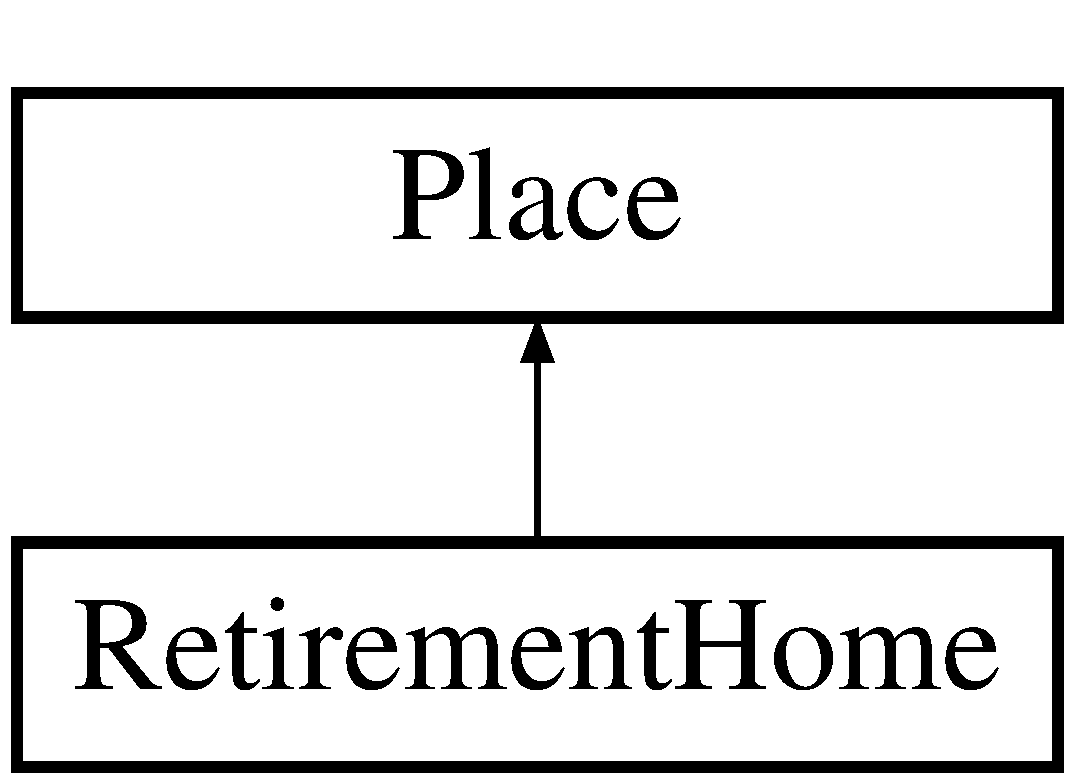
\includegraphics[height=2.000000cm]{classRetirementHome}
\end{center}
\end{figure}
\subsection*{Public Member Functions}
\begin{DoxyCompactItemize}
\item 
\hyperlink{classRetirementHome_a9161850a079e6f54e129eeceb5fedf37}{Retirement\+Home} ()=default
\begin{DoxyCompactList}\small\item\em Creates a \hyperlink{classRetirementHome}{Retirement\+Home} object with default attributes. \end{DoxyCompactList}\item 
\hyperlink{classRetirementHome_a31e01ecb1d6a99468939ed75090803ef}{Retirement\+Home} (const int rh\+\_\+\+ID, const double xi, const double yi, const double severity\+\_\+cor, const double psi\+\_\+e, const double beta\+\_\+e, const double beta\+\_\+r, const double betaih)
\begin{DoxyCompactList}\small\item\em Creates a \hyperlink{classRetirementHome}{Retirement\+Home} object. \end{DoxyCompactList}\item 
void \hyperlink{classRetirementHome_a7b2c07f448001eff03b70fc460701fbd}{add\+\_\+exposed\+\_\+employee} (double inf\+\_\+var)
\begin{DoxyCompactList}\small\item\em Include exposed employee contribution in the sum. \end{DoxyCompactList}\item 
void \hyperlink{classRetirementHome_ab2a24b8583ae1e34cc8baf2d04c27116}{add\+\_\+symptomatic\+\_\+employee} (double inf\+\_\+var)
\begin{DoxyCompactList}\small\item\em Include symptomatic employee contribution in the sum. \end{DoxyCompactList}\item 
void \hyperlink{classRetirementHome_a8c7f00431e809d16b335d18daf512df1}{add\+\_\+symptomatic\+\_\+home\+\_\+isolated} (double inf\+\_\+var)
\begin{DoxyCompactList}\small\item\em Include contribution of a symptomatic, home isolated agent in the sum. \end{DoxyCompactList}\item 
void \hyperlink{classRetirementHome_aaa3cd3799f2c48c92d5265bcfe514640}{add\+\_\+exposed\+\_\+home\+\_\+isolated} (double inf\+\_\+var)
\begin{DoxyCompactList}\small\item\em Include contribution of an exposed, home isolated agent in the sum. \end{DoxyCompactList}\item 
void \hyperlink{classRetirementHome_aafab41675600b03fdffcf11db1a07ec7}{print\+\_\+basic} (std\+::ostream \&where) const override
\begin{DoxyCompactList}\small\item\em Save information about a \hyperlink{classRetirementHome}{Retirement\+Home} object. \end{DoxyCompactList}\end{DoxyCompactItemize}
\subsection*{Additional Inherited Members}


\subsection{Constructor \& Destructor Documentation}
\mbox{\Hypertarget{classRetirementHome_a9161850a079e6f54e129eeceb5fedf37}\label{classRetirementHome_a9161850a079e6f54e129eeceb5fedf37}} 
\index{Retirement\+Home@{Retirement\+Home}!Retirement\+Home@{Retirement\+Home}}
\index{Retirement\+Home@{Retirement\+Home}!Retirement\+Home@{Retirement\+Home}}
\subsubsection{\texorpdfstring{Retirement\+Home()}{RetirementHome()}\hspace{0.1cm}{\footnotesize\ttfamily [1/2]}}
{\footnotesize\ttfamily Retirement\+Home\+::\+Retirement\+Home (\begin{DoxyParamCaption}{ }\end{DoxyParamCaption})\hspace{0.3cm}{\ttfamily [default]}}



Creates a \hyperlink{classRetirementHome}{Retirement\+Home} object with default attributes. 

\mbox{\Hypertarget{classRetirementHome_a31e01ecb1d6a99468939ed75090803ef}\label{classRetirementHome_a31e01ecb1d6a99468939ed75090803ef}} 
\index{Retirement\+Home@{Retirement\+Home}!Retirement\+Home@{Retirement\+Home}}
\index{Retirement\+Home@{Retirement\+Home}!Retirement\+Home@{Retirement\+Home}}
\subsubsection{\texorpdfstring{Retirement\+Home()}{RetirementHome()}\hspace{0.1cm}{\footnotesize\ttfamily [2/2]}}
{\footnotesize\ttfamily Retirement\+Home\+::\+Retirement\+Home (\begin{DoxyParamCaption}\item[{const int}]{rh\+\_\+\+ID,  }\item[{const double}]{xi,  }\item[{const double}]{yi,  }\item[{const double}]{severity\+\_\+cor,  }\item[{const double}]{psi\+\_\+e,  }\item[{const double}]{beta\+\_\+e,  }\item[{const double}]{beta\+\_\+r,  }\item[{const double}]{betaih }\end{DoxyParamCaption})\hspace{0.3cm}{\ttfamily [inline]}}



Creates a \hyperlink{classRetirementHome}{Retirement\+Home} object. 

Retirement home with custom ID, location, and infection parameters


\begin{DoxyParams}{Parameters}
{\em rh\+\_\+\+ID} & -\/ ID of the home \\
\hline
{\em xi} & -\/ x coordinate of the home \\
\hline
{\em yi} & -\/ y coordinate of the home \\
\hline
{\em severity\+\_\+cor} & -\/ severity correction for symptomatic \\
\hline
{\em psi\+\_\+e} & -\/ employee absenteeism correction \\
\hline
{\em beta\+\_\+e} & -\/ employee infection transmission rate, 1/time \\
\hline
{\em beta\+\_\+r} & -\/ resident infection transmission rate, 1/time \\
\hline
{\em betaih} & -\/ infection transmission rate for home isolated, 1/time \\
\hline
\end{DoxyParams}


\subsection{Member Function Documentation}
\mbox{\Hypertarget{classRetirementHome_a7b2c07f448001eff03b70fc460701fbd}\label{classRetirementHome_a7b2c07f448001eff03b70fc460701fbd}} 
\index{Retirement\+Home@{Retirement\+Home}!add\+\_\+exposed\+\_\+employee@{add\+\_\+exposed\+\_\+employee}}
\index{add\+\_\+exposed\+\_\+employee@{add\+\_\+exposed\+\_\+employee}!Retirement\+Home@{Retirement\+Home}}
\subsubsection{\texorpdfstring{add\+\_\+exposed\+\_\+employee()}{add\_exposed\_employee()}}
{\footnotesize\ttfamily void Retirement\+Home\+::add\+\_\+exposed\+\_\+employee (\begin{DoxyParamCaption}\item[{double}]{inf\+\_\+var }\end{DoxyParamCaption})\hspace{0.3cm}{\ttfamily [inline]}}



Include exposed employee contribution in the sum. 


\begin{DoxyParams}{Parameters}
{\em inf\+\_\+var} & -\/ agent infectiousness variability factor \\
\hline
\end{DoxyParams}
\mbox{\Hypertarget{classRetirementHome_aaa3cd3799f2c48c92d5265bcfe514640}\label{classRetirementHome_aaa3cd3799f2c48c92d5265bcfe514640}} 
\index{Retirement\+Home@{Retirement\+Home}!add\+\_\+exposed\+\_\+home\+\_\+isolated@{add\+\_\+exposed\+\_\+home\+\_\+isolated}}
\index{add\+\_\+exposed\+\_\+home\+\_\+isolated@{add\+\_\+exposed\+\_\+home\+\_\+isolated}!Retirement\+Home@{Retirement\+Home}}
\subsubsection{\texorpdfstring{add\+\_\+exposed\+\_\+home\+\_\+isolated()}{add\_exposed\_home\_isolated()}}
{\footnotesize\ttfamily void Retirement\+Home\+::add\+\_\+exposed\+\_\+home\+\_\+isolated (\begin{DoxyParamCaption}\item[{double}]{inf\+\_\+var }\end{DoxyParamCaption})\hspace{0.3cm}{\ttfamily [inline]}}



Include contribution of an exposed, home isolated agent in the sum. 


\begin{DoxyParams}{Parameters}
{\em inf\+\_\+var} & -\/ agent infectiousness variability factor \\
\hline
\end{DoxyParams}
\mbox{\Hypertarget{classRetirementHome_ab2a24b8583ae1e34cc8baf2d04c27116}\label{classRetirementHome_ab2a24b8583ae1e34cc8baf2d04c27116}} 
\index{Retirement\+Home@{Retirement\+Home}!add\+\_\+symptomatic\+\_\+employee@{add\+\_\+symptomatic\+\_\+employee}}
\index{add\+\_\+symptomatic\+\_\+employee@{add\+\_\+symptomatic\+\_\+employee}!Retirement\+Home@{Retirement\+Home}}
\subsubsection{\texorpdfstring{add\+\_\+symptomatic\+\_\+employee()}{add\_symptomatic\_employee()}}
{\footnotesize\ttfamily void Retirement\+Home\+::add\+\_\+symptomatic\+\_\+employee (\begin{DoxyParamCaption}\item[{double}]{inf\+\_\+var }\end{DoxyParamCaption})\hspace{0.3cm}{\ttfamily [inline]}}



Include symptomatic employee contribution in the sum. 


\begin{DoxyParams}{Parameters}
{\em inf\+\_\+var} & -\/ agent infectiousness variability factor \\
\hline
\end{DoxyParams}
\mbox{\Hypertarget{classRetirementHome_a8c7f00431e809d16b335d18daf512df1}\label{classRetirementHome_a8c7f00431e809d16b335d18daf512df1}} 
\index{Retirement\+Home@{Retirement\+Home}!add\+\_\+symptomatic\+\_\+home\+\_\+isolated@{add\+\_\+symptomatic\+\_\+home\+\_\+isolated}}
\index{add\+\_\+symptomatic\+\_\+home\+\_\+isolated@{add\+\_\+symptomatic\+\_\+home\+\_\+isolated}!Retirement\+Home@{Retirement\+Home}}
\subsubsection{\texorpdfstring{add\+\_\+symptomatic\+\_\+home\+\_\+isolated()}{add\_symptomatic\_home\_isolated()}}
{\footnotesize\ttfamily void Retirement\+Home\+::add\+\_\+symptomatic\+\_\+home\+\_\+isolated (\begin{DoxyParamCaption}\item[{double}]{inf\+\_\+var }\end{DoxyParamCaption})\hspace{0.3cm}{\ttfamily [inline]}}



Include contribution of a symptomatic, home isolated agent in the sum. 


\begin{DoxyParams}{Parameters}
{\em inf\+\_\+var} & -\/ agent infectiousness variability factor \\
\hline
\end{DoxyParams}
\mbox{\Hypertarget{classRetirementHome_aafab41675600b03fdffcf11db1a07ec7}\label{classRetirementHome_aafab41675600b03fdffcf11db1a07ec7}} 
\index{Retirement\+Home@{Retirement\+Home}!print\+\_\+basic@{print\+\_\+basic}}
\index{print\+\_\+basic@{print\+\_\+basic}!Retirement\+Home@{Retirement\+Home}}
\subsubsection{\texorpdfstring{print\+\_\+basic()}{print\_basic()}}
{\footnotesize\ttfamily void Retirement\+Home\+::print\+\_\+basic (\begin{DoxyParamCaption}\item[{std\+::ostream \&}]{where }\end{DoxyParamCaption}) const\hspace{0.3cm}{\ttfamily [override]}, {\ttfamily [virtual]}}



Save information about a \hyperlink{classRetirementHome}{Retirement\+Home} object. 

Saves to a file, everything but detailed agent information; order is ID $\vert$ x $\vert$ y $\vert$ number of agents $\vert$ number of infected agents $\vert$ ck $\vert$ betas $\vert$ psis Delimiter is a space. 
\begin{DoxyParams}{Parameters}
{\em where} & -\/ output stream \\
\hline
\end{DoxyParams}


Reimplemented from \hyperlink{classPlace_a9aa7649e0b91c5f61a5f71e9ca808fe1}{Place}.



The documentation for this class was generated from the following files\+:\begin{DoxyCompactItemize}
\item 
include/places/\hyperlink{retirement__home_8h}{retirement\+\_\+home.\+h}\item 
src/places/\hyperlink{retirement__home_8cpp}{retirement\+\_\+home.\+cpp}\end{DoxyCompactItemize}

\hypertarget{classRNG}{}\section{R\+NG Class Reference}
\label{classRNG}\index{R\+NG@{R\+NG}}


{\ttfamily \#include $<$rng.\+h$>$}

\subsection*{Public Member Functions}
\begin{DoxyCompactItemize}
\item 
\hyperlink{classRNG_a0028b717ff3d402a5829fc09ab1c5ed4}{R\+NG} ()
\item 
double \hyperlink{classRNG_a9c2ed7323632e3bade78543f3455d055}{get\+\_\+random} (const double dmin, const double dmax)
\begin{DoxyCompactList}\small\item\em Random number sampled from uniform distribution. \end{DoxyCompactList}\item 
int \hyperlink{classRNG_a9f4c1cb8ca99c2838de7077f2a0c48ef}{get\+\_\+random\+\_\+int} (const int dmin, const int dmax)
\begin{DoxyCompactList}\small\item\em Random integer sampled from uniform distribution of ints. \end{DoxyCompactList}\item 
double \hyperlink{classRNG_ad4c8f00da1722cad6c57873ecc45187d}{get\+\_\+random\+\_\+gamma} (const double k, const double theta)
\begin{DoxyCompactList}\small\item\em Random number sampled from a gamma distribution. \end{DoxyCompactList}\item 
double \hyperlink{classRNG_a45c08c830077f4ad9c9a41ec2ab36021}{get\+\_\+random\+\_\+lognormal} (const double m, const double s)
\begin{DoxyCompactList}\small\item\em Random number sampled from a lognormal distribution. \end{DoxyCompactList}\item 
double \hyperlink{classRNG_ae7be35e443ee86c915b32fdfc2595187}{get\+\_\+random\+\_\+weibull} (const double a, const double b)
\begin{DoxyCompactList}\small\item\em Random number sampled from a Weibull distribution. \end{DoxyCompactList}\item 
void \hyperlink{classRNG_ad1fb3455e12c12637e74c9673984496d}{vector\+\_\+shuffle} (std\+::vector$<$ int $>$ \&v)
\begin{DoxyCompactList}\small\item\em Performs in-\/place random shuffling of a vector. \end{DoxyCompactList}\end{DoxyCompactItemize}


\subsection{Constructor \& Destructor Documentation}
\mbox{\Hypertarget{classRNG_a0028b717ff3d402a5829fc09ab1c5ed4}\label{classRNG_a0028b717ff3d402a5829fc09ab1c5ed4}} 
\index{R\+NG@{R\+NG}!R\+NG@{R\+NG}}
\index{R\+NG@{R\+NG}!R\+NG@{R\+NG}}
\subsubsection{\texorpdfstring{R\+N\+G()}{RNG()}}
{\footnotesize\ttfamily R\+N\+G\+::\+R\+NG (\begin{DoxyParamCaption}{ }\end{DoxyParamCaption})\hspace{0.3cm}{\ttfamily [inline]}}



\subsection{Member Function Documentation}
\mbox{\Hypertarget{classRNG_a9c2ed7323632e3bade78543f3455d055}\label{classRNG_a9c2ed7323632e3bade78543f3455d055}} 
\index{R\+NG@{R\+NG}!get\+\_\+random@{get\+\_\+random}}
\index{get\+\_\+random@{get\+\_\+random}!R\+NG@{R\+NG}}
\subsubsection{\texorpdfstring{get\+\_\+random()}{get\_random()}}
{\footnotesize\ttfamily double R\+N\+G\+::get\+\_\+random (\begin{DoxyParamCaption}\item[{const double}]{dmin,  }\item[{const double}]{dmax }\end{DoxyParamCaption})\hspace{0.3cm}{\ttfamily [inline]}}



Random number sampled from uniform distribution. 


\begin{DoxyParams}{Parameters}
{\em dmin} & -\/ minimum, inclusive \\
\hline
{\em dmax} & -\/ maximum, exclusive \\
\hline
\end{DoxyParams}
\mbox{\Hypertarget{classRNG_ad4c8f00da1722cad6c57873ecc45187d}\label{classRNG_ad4c8f00da1722cad6c57873ecc45187d}} 
\index{R\+NG@{R\+NG}!get\+\_\+random\+\_\+gamma@{get\+\_\+random\+\_\+gamma}}
\index{get\+\_\+random\+\_\+gamma@{get\+\_\+random\+\_\+gamma}!R\+NG@{R\+NG}}
\subsubsection{\texorpdfstring{get\+\_\+random\+\_\+gamma()}{get\_random\_gamma()}}
{\footnotesize\ttfamily double R\+N\+G\+::get\+\_\+random\+\_\+gamma (\begin{DoxyParamCaption}\item[{const double}]{k,  }\item[{const double}]{theta }\end{DoxyParamCaption})\hspace{0.3cm}{\ttfamily [inline]}}



Random number sampled from a gamma distribution. 


\begin{DoxyParams}{Parameters}
{\em k} & -\/ shape parameter \\
\hline
{\em theta} & -\/ scale parameter \\
\hline
\end{DoxyParams}
\mbox{\Hypertarget{classRNG_a9f4c1cb8ca99c2838de7077f2a0c48ef}\label{classRNG_a9f4c1cb8ca99c2838de7077f2a0c48ef}} 
\index{R\+NG@{R\+NG}!get\+\_\+random\+\_\+int@{get\+\_\+random\+\_\+int}}
\index{get\+\_\+random\+\_\+int@{get\+\_\+random\+\_\+int}!R\+NG@{R\+NG}}
\subsubsection{\texorpdfstring{get\+\_\+random\+\_\+int()}{get\_random\_int()}}
{\footnotesize\ttfamily int R\+N\+G\+::get\+\_\+random\+\_\+int (\begin{DoxyParamCaption}\item[{const int}]{dmin,  }\item[{const int}]{dmax }\end{DoxyParamCaption})\hspace{0.3cm}{\ttfamily [inline]}}



Random integer sampled from uniform distribution of ints. 


\begin{DoxyParams}{Parameters}
{\em dmin} & -\/ minimum, inclusive \\
\hline
{\em dmax} & -\/ maximum, inclusive \\
\hline
\end{DoxyParams}
\mbox{\Hypertarget{classRNG_a45c08c830077f4ad9c9a41ec2ab36021}\label{classRNG_a45c08c830077f4ad9c9a41ec2ab36021}} 
\index{R\+NG@{R\+NG}!get\+\_\+random\+\_\+lognormal@{get\+\_\+random\+\_\+lognormal}}
\index{get\+\_\+random\+\_\+lognormal@{get\+\_\+random\+\_\+lognormal}!R\+NG@{R\+NG}}
\subsubsection{\texorpdfstring{get\+\_\+random\+\_\+lognormal()}{get\_random\_lognormal()}}
{\footnotesize\ttfamily double R\+N\+G\+::get\+\_\+random\+\_\+lognormal (\begin{DoxyParamCaption}\item[{const double}]{m,  }\item[{const double}]{s }\end{DoxyParamCaption})\hspace{0.3cm}{\ttfamily [inline]}}



Random number sampled from a lognormal distribution. 


\begin{DoxyParams}{Parameters}
{\em m} & -\/ mean \\
\hline
{\em s} & -\/ standard deviation \\
\hline
\end{DoxyParams}
\mbox{\Hypertarget{classRNG_ae7be35e443ee86c915b32fdfc2595187}\label{classRNG_ae7be35e443ee86c915b32fdfc2595187}} 
\index{R\+NG@{R\+NG}!get\+\_\+random\+\_\+weibull@{get\+\_\+random\+\_\+weibull}}
\index{get\+\_\+random\+\_\+weibull@{get\+\_\+random\+\_\+weibull}!R\+NG@{R\+NG}}
\subsubsection{\texorpdfstring{get\+\_\+random\+\_\+weibull()}{get\_random\_weibull()}}
{\footnotesize\ttfamily double R\+N\+G\+::get\+\_\+random\+\_\+weibull (\begin{DoxyParamCaption}\item[{const double}]{a,  }\item[{const double}]{b }\end{DoxyParamCaption})\hspace{0.3cm}{\ttfamily [inline]}}



Random number sampled from a Weibull distribution. 


\begin{DoxyParams}{Parameters}
{\em a} & -\/ shape parameter \\
\hline
{\em b} & -\/ scale parameter \\
\hline
\end{DoxyParams}
\mbox{\Hypertarget{classRNG_ad1fb3455e12c12637e74c9673984496d}\label{classRNG_ad1fb3455e12c12637e74c9673984496d}} 
\index{R\+NG@{R\+NG}!vector\+\_\+shuffle@{vector\+\_\+shuffle}}
\index{vector\+\_\+shuffle@{vector\+\_\+shuffle}!R\+NG@{R\+NG}}
\subsubsection{\texorpdfstring{vector\+\_\+shuffle()}{vector\_shuffle()}}
{\footnotesize\ttfamily void R\+N\+G\+::vector\+\_\+shuffle (\begin{DoxyParamCaption}\item[{std\+::vector$<$ int $>$ \&}]{v }\end{DoxyParamCaption})\hspace{0.3cm}{\ttfamily [inline]}}



Performs in-\/place random shuffling of a vector. 



The documentation for this class was generated from the following file\+:\begin{DoxyCompactItemize}
\item 
include/\hyperlink{rng_8h}{rng.\+h}\end{DoxyCompactItemize}

\hypertarget{classSchool}{}\section{School Class Reference}
\label{classSchool}\index{School@{School}}


{\ttfamily \#include $<$school.\+h$>$}

Inheritance diagram for School\+:\begin{figure}[H]
\begin{center}
\leavevmode
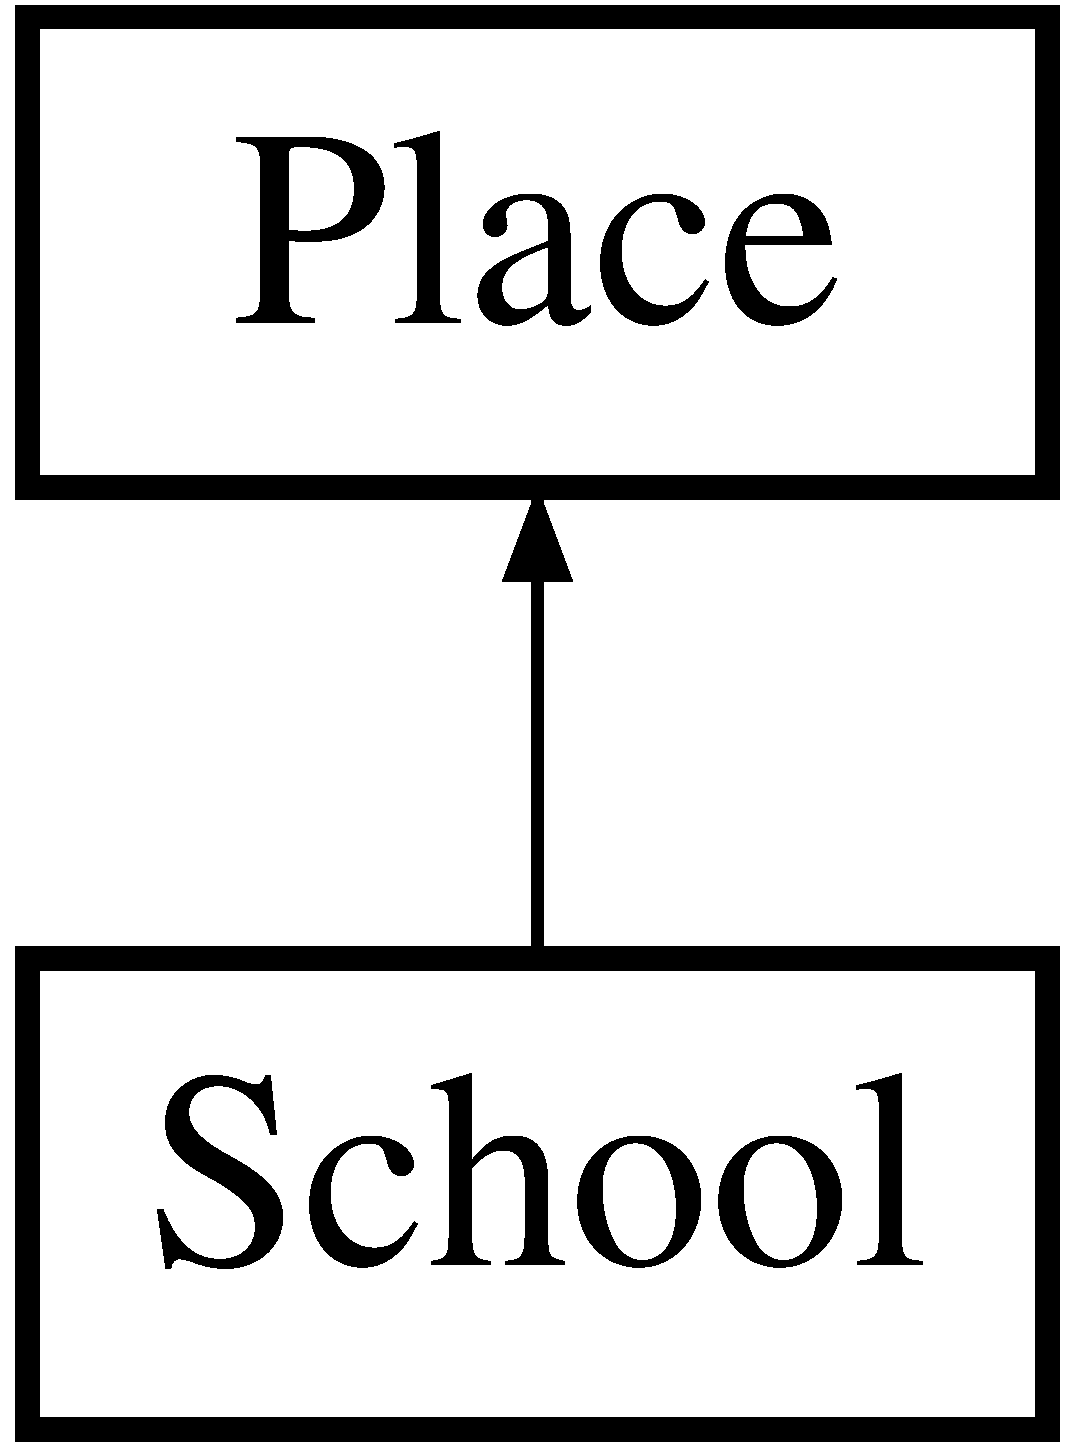
\includegraphics[height=2.000000cm]{classSchool}
\end{center}
\end{figure}
\subsection*{Public Member Functions}
\begin{DoxyCompactItemize}
\item 
\hyperlink{classSchool_a18efa7137fe6c142ababf7d4ed838a07}{School} ()=default
\begin{DoxyCompactList}\small\item\em Creates a \hyperlink{classSchool}{School} object with default attributes. \end{DoxyCompactList}\item 
\hyperlink{classSchool_a4f9cd6dacc298715885c917b8a14e4ca}{School} (const int school\+\_\+\+ID, const double xi, const double yi, const double severity\+\_\+cor, const double psi\+\_\+e, const double psi, const double beta\+\_\+e, const double beta\+\_\+s)
\begin{DoxyCompactList}\small\item\em Creates a \hyperlink{classSchool}{School} object. \end{DoxyCompactList}\item 
void \hyperlink{classSchool_aa3d7bde17fc920efc33f3152f3df5671}{add\+\_\+exposed\+\_\+employee} (double inf\+\_\+var)
\begin{DoxyCompactList}\small\item\em Include exposed employee contribution in the sum. \end{DoxyCompactList}\item 
void \hyperlink{classSchool_aaa75cfbde33ca728de63c9d6f72b1ff8}{add\+\_\+symptomatic\+\_\+employee} (double inf\+\_\+var)
\begin{DoxyCompactList}\small\item\em Include symptomatic employee contribution in the sum. \end{DoxyCompactList}\item 
void \hyperlink{classSchool_ac5457e1834cbf399c4c9ad8a6971673f}{add\+\_\+symptomatic\+\_\+student} (double inf\+\_\+var)
\begin{DoxyCompactList}\small\item\em Include symptomatic student contribution in the sum. \end{DoxyCompactList}\item 
void \hyperlink{classSchool_aba41cef9af3f2cb98bf1075c289baf84}{change\+\_\+employee\+\_\+transmission\+\_\+rate} (const double new\+\_\+rate)
\item 
double \hyperlink{classSchool_a7cc6659bce874d0cc56ed45972c7d842}{get\+\_\+employee\+\_\+transmission\+\_\+rate} () const
\item 
void \hyperlink{classSchool_ade1610f7c072eb041f6d8b0e157e1cc8}{print\+\_\+basic} (std\+::ostream \&where) const override
\begin{DoxyCompactList}\small\item\em Save information about a \hyperlink{classSchool}{School} object. \end{DoxyCompactList}\end{DoxyCompactItemize}
\subsection*{Additional Inherited Members}


\subsection{Constructor \& Destructor Documentation}
\mbox{\Hypertarget{classSchool_a18efa7137fe6c142ababf7d4ed838a07}\label{classSchool_a18efa7137fe6c142ababf7d4ed838a07}} 
\index{School@{School}!School@{School}}
\index{School@{School}!School@{School}}
\subsubsection{\texorpdfstring{School()}{School()}\hspace{0.1cm}{\footnotesize\ttfamily [1/2]}}
{\footnotesize\ttfamily School\+::\+School (\begin{DoxyParamCaption}{ }\end{DoxyParamCaption})\hspace{0.3cm}{\ttfamily [default]}}



Creates a \hyperlink{classSchool}{School} object with default attributes. 

\mbox{\Hypertarget{classSchool_a4f9cd6dacc298715885c917b8a14e4ca}\label{classSchool_a4f9cd6dacc298715885c917b8a14e4ca}} 
\index{School@{School}!School@{School}}
\index{School@{School}!School@{School}}
\subsubsection{\texorpdfstring{School()}{School()}\hspace{0.1cm}{\footnotesize\ttfamily [2/2]}}
{\footnotesize\ttfamily School\+::\+School (\begin{DoxyParamCaption}\item[{const int}]{school\+\_\+\+ID,  }\item[{const double}]{xi,  }\item[{const double}]{yi,  }\item[{const double}]{severity\+\_\+cor,  }\item[{const double}]{psi\+\_\+e,  }\item[{const double}]{psi,  }\item[{const double}]{beta\+\_\+e,  }\item[{const double}]{beta\+\_\+s }\end{DoxyParamCaption})\hspace{0.3cm}{\ttfamily [inline]}}



Creates a \hyperlink{classSchool}{School} object. 

\hyperlink{classSchool}{School} with custom ID, location, and infection parameters


\begin{DoxyParams}{Parameters}
{\em school\+\_\+\+ID} & -\/ ID of the school \\
\hline
{\em xi} & -\/ x coordinate of the school \\
\hline
{\em yi} & -\/ y coordinate of the school \\
\hline
{\em severity\+\_\+cor} & -\/ severity correction for symptomatic \\
\hline
{\em psi\+\_\+e} & -\/ employee absenteeism correction \\
\hline
{\em psi} & -\/ student absenteeism correction \\
\hline
{\em beta\+\_\+e} & -\/ employee infection transmission rate, 1/time \\
\hline
{\em beta\+\_\+s} & -\/ student infection transmission rate, 1/time \\
\hline
\end{DoxyParams}


\subsection{Member Function Documentation}
\mbox{\Hypertarget{classSchool_aa3d7bde17fc920efc33f3152f3df5671}\label{classSchool_aa3d7bde17fc920efc33f3152f3df5671}} 
\index{School@{School}!add\+\_\+exposed\+\_\+employee@{add\+\_\+exposed\+\_\+employee}}
\index{add\+\_\+exposed\+\_\+employee@{add\+\_\+exposed\+\_\+employee}!School@{School}}
\subsubsection{\texorpdfstring{add\+\_\+exposed\+\_\+employee()}{add\_exposed\_employee()}}
{\footnotesize\ttfamily void School\+::add\+\_\+exposed\+\_\+employee (\begin{DoxyParamCaption}\item[{double}]{inf\+\_\+var }\end{DoxyParamCaption})\hspace{0.3cm}{\ttfamily [inline]}}



Include exposed employee contribution in the sum. 


\begin{DoxyParams}{Parameters}
{\em inf\+\_\+var} & -\/ agent infectiousness variability factor \\
\hline
\end{DoxyParams}
\mbox{\Hypertarget{classSchool_aaa75cfbde33ca728de63c9d6f72b1ff8}\label{classSchool_aaa75cfbde33ca728de63c9d6f72b1ff8}} 
\index{School@{School}!add\+\_\+symptomatic\+\_\+employee@{add\+\_\+symptomatic\+\_\+employee}}
\index{add\+\_\+symptomatic\+\_\+employee@{add\+\_\+symptomatic\+\_\+employee}!School@{School}}
\subsubsection{\texorpdfstring{add\+\_\+symptomatic\+\_\+employee()}{add\_symptomatic\_employee()}}
{\footnotesize\ttfamily void School\+::add\+\_\+symptomatic\+\_\+employee (\begin{DoxyParamCaption}\item[{double}]{inf\+\_\+var }\end{DoxyParamCaption})\hspace{0.3cm}{\ttfamily [inline]}}



Include symptomatic employee contribution in the sum. 


\begin{DoxyParams}{Parameters}
{\em inf\+\_\+var} & -\/ agent infectiousness variability factor \\
\hline
\end{DoxyParams}
\mbox{\Hypertarget{classSchool_ac5457e1834cbf399c4c9ad8a6971673f}\label{classSchool_ac5457e1834cbf399c4c9ad8a6971673f}} 
\index{School@{School}!add\+\_\+symptomatic\+\_\+student@{add\+\_\+symptomatic\+\_\+student}}
\index{add\+\_\+symptomatic\+\_\+student@{add\+\_\+symptomatic\+\_\+student}!School@{School}}
\subsubsection{\texorpdfstring{add\+\_\+symptomatic\+\_\+student()}{add\_symptomatic\_student()}}
{\footnotesize\ttfamily void School\+::add\+\_\+symptomatic\+\_\+student (\begin{DoxyParamCaption}\item[{double}]{inf\+\_\+var }\end{DoxyParamCaption})\hspace{0.3cm}{\ttfamily [inline]}}



Include symptomatic student contribution in the sum. 


\begin{DoxyParams}{Parameters}
{\em inf\+\_\+var} & -\/ agent infectiousness variability factor \\
\hline
\end{DoxyParams}
\mbox{\Hypertarget{classSchool_aba41cef9af3f2cb98bf1075c289baf84}\label{classSchool_aba41cef9af3f2cb98bf1075c289baf84}} 
\index{School@{School}!change\+\_\+employee\+\_\+transmission\+\_\+rate@{change\+\_\+employee\+\_\+transmission\+\_\+rate}}
\index{change\+\_\+employee\+\_\+transmission\+\_\+rate@{change\+\_\+employee\+\_\+transmission\+\_\+rate}!School@{School}}
\subsubsection{\texorpdfstring{change\+\_\+employee\+\_\+transmission\+\_\+rate()}{change\_employee\_transmission\_rate()}}
{\footnotesize\ttfamily void School\+::change\+\_\+employee\+\_\+transmission\+\_\+rate (\begin{DoxyParamCaption}\item[{const double}]{new\+\_\+rate }\end{DoxyParamCaption})\hspace{0.3cm}{\ttfamily [inline]}}

\mbox{\Hypertarget{classSchool_a7cc6659bce874d0cc56ed45972c7d842}\label{classSchool_a7cc6659bce874d0cc56ed45972c7d842}} 
\index{School@{School}!get\+\_\+employee\+\_\+transmission\+\_\+rate@{get\+\_\+employee\+\_\+transmission\+\_\+rate}}
\index{get\+\_\+employee\+\_\+transmission\+\_\+rate@{get\+\_\+employee\+\_\+transmission\+\_\+rate}!School@{School}}
\subsubsection{\texorpdfstring{get\+\_\+employee\+\_\+transmission\+\_\+rate()}{get\_employee\_transmission\_rate()}}
{\footnotesize\ttfamily double School\+::get\+\_\+employee\+\_\+transmission\+\_\+rate (\begin{DoxyParamCaption}{ }\end{DoxyParamCaption}) const\hspace{0.3cm}{\ttfamily [inline]}}

\mbox{\Hypertarget{classSchool_ade1610f7c072eb041f6d8b0e157e1cc8}\label{classSchool_ade1610f7c072eb041f6d8b0e157e1cc8}} 
\index{School@{School}!print\+\_\+basic@{print\+\_\+basic}}
\index{print\+\_\+basic@{print\+\_\+basic}!School@{School}}
\subsubsection{\texorpdfstring{print\+\_\+basic()}{print\_basic()}}
{\footnotesize\ttfamily void School\+::print\+\_\+basic (\begin{DoxyParamCaption}\item[{std\+::ostream \&}]{where }\end{DoxyParamCaption}) const\hspace{0.3cm}{\ttfamily [override]}, {\ttfamily [virtual]}}



Save information about a \hyperlink{classSchool}{School} object. 

Saves to a file, everything but detailed agent information; order is ID $\vert$ x $\vert$ y $\vert$ number of agents $\vert$ number of infected agents $\vert$ ck $\vert$ betas $\vert$ psis Delimiter is a space. 
\begin{DoxyParams}{Parameters}
{\em where} & -\/ output stream \\
\hline
\end{DoxyParams}


Reimplemented from \hyperlink{classPlace_a9aa7649e0b91c5f61a5f71e9ca808fe1}{Place}.



The documentation for this class was generated from the following files\+:\begin{DoxyCompactItemize}
\item 
include/places/\hyperlink{school_8h}{school.\+h}\item 
src/places/\hyperlink{school_8cpp}{school.\+cpp}\end{DoxyCompactItemize}

\hypertarget{classStatesManager}{}\section{States\+Manager Class Reference}
\label{classStatesManager}\index{States\+Manager@{States\+Manager}}


{\ttfamily \#include $<$states\+\_\+manager.\+h$>$}

\subsection*{Public Member Functions}
\begin{DoxyCompactItemize}
\item 
\hyperlink{classStatesManager_a9aa295a6122b9501a24e3ef4449c660f}{States\+Manager} ()=default
\item 
void \hyperlink{classStatesManager_a3b2001cf1da5e448c7d2f08bba30d05b}{set\+\_\+susceptible\+\_\+to\+\_\+exposed} (\hyperlink{classAgent}{Agent} \&agent)
\begin{DoxyCompactList}\small\item\em Set all states for transition from susceptible to exposed. \end{DoxyCompactList}\item 
void \hyperlink{classStatesManager_a1d6cbcb237b03565c83f4f618da08cbe}{set\+\_\+susceptible\+\_\+to\+\_\+exposed\+\_\+never\+\_\+symptomatic} (\hyperlink{classAgent}{Agent} \&agent)
\begin{DoxyCompactList}\small\item\em Set all states for transition from susceptible to exposed that will never become symptomatic. \end{DoxyCompactList}\item 
void \hyperlink{classStatesManager_a70153bfe33b4fde44c950a0d6eac5191}{set\+\_\+exposed\+\_\+never\+\_\+symptomatic\+\_\+to\+\_\+removed} (\hyperlink{classAgent}{Agent} \&agent)
\begin{DoxyCompactList}\small\item\em Set exposed that never developed symptoms to removed. \end{DoxyCompactList}\item 
void \hyperlink{classStatesManager_a675b30619c98f0c4743d08aba0567dad}{set\+\_\+exposed\+\_\+to\+\_\+symptomatic} (\hyperlink{classAgent}{Agent} \&agent)
\begin{DoxyCompactList}\small\item\em Set all states for transition from exposed to general symptomatic. \end{DoxyCompactList}\item 
void \hyperlink{classStatesManager_adcd6bc8a8f260efcf7cf43dcebe0334e}{set\+\_\+dying\+\_\+symptomatic} (\hyperlink{classAgent}{Agent} \&agent)
\begin{DoxyCompactList}\small\item\em Set all states relevant to agent that will die. \end{DoxyCompactList}\item 
void \hyperlink{classStatesManager_a01294a7aead97c9d002f202093051b81}{set\+\_\+recovering\+\_\+symptomatic} (\hyperlink{classAgent}{Agent} \&agent)
\begin{DoxyCompactList}\small\item\em Set all states relevant to agent that will recover. \end{DoxyCompactList}\item 
void \hyperlink{classStatesManager_ac3900f6b45182c5ba0103bb524df769a}{set\+\_\+waiting\+\_\+for\+\_\+test\+\_\+in\+\_\+hospital} (\hyperlink{classAgent}{Agent} \&agent)
\begin{DoxyCompactList}\small\item\em Set testing in hospital, initial state. \end{DoxyCompactList}\item 
void \hyperlink{classStatesManager_a280373c96ad5df8a9044235be2351556}{set\+\_\+waiting\+\_\+for\+\_\+test\+\_\+in\+\_\+car} (\hyperlink{classAgent}{Agent} \&agent)
\begin{DoxyCompactList}\small\item\em Set testing in a car, initial state. \end{DoxyCompactList}\item 
void \hyperlink{classStatesManager_aaf0cfd7137a490fc716af5ff5dbb4bcd}{set\+\_\+tested\+\_\+to\+\_\+awaiting\+\_\+results} (\hyperlink{classAgent}{Agent} \&agent)
\begin{DoxyCompactList}\small\item\em Set all states for just tested. \end{DoxyCompactList}\item 
void \hyperlink{classStatesManager_ad6f9193dcf05f4f37e71a94d58315481}{set\+\_\+tested\+\_\+false\+\_\+negative} (\hyperlink{classAgent}{Agent} \&agent)
\begin{DoxyCompactList}\small\item\em Set all states for transition from tested to false negative. \end{DoxyCompactList}\item 
void \hyperlink{classStatesManager_a2044045b6b2adc1a94b5d02f72272cb7}{set\+\_\+icu\+\_\+dying} (\hyperlink{classAgent}{Agent} \&agent)
\begin{DoxyCompactList}\small\item\em States for hospitalized, I\+CU -\/ dying. \end{DoxyCompactList}\item 
void \hyperlink{classStatesManager_a4c182f0f50b7f9355ef5799a5623a5d0}{set\+\_\+icu\+\_\+recovering} (\hyperlink{classAgent}{Agent} \&agent)
\begin{DoxyCompactList}\small\item\em States for hospitalized, I\+CU -\/ recovering. \end{DoxyCompactList}\item 
void \hyperlink{classStatesManager_a266757d7944ac2a13ec122e563fcfd0d}{set\+\_\+hospitalized} (\hyperlink{classAgent}{Agent} \&agent)
\begin{DoxyCompactList}\small\item\em States for hospitalized. \end{DoxyCompactList}\item 
void \hyperlink{classStatesManager_a5660eb874c13cabb0af244f8c6768685}{set\+\_\+home\+\_\+isolation} (\hyperlink{classAgent}{Agent} \&agent)
\begin{DoxyCompactList}\small\item\em States for isolated at home. \end{DoxyCompactList}\item 
void \hyperlink{classStatesManager_af64b9d50a965045094e39fb4a6e25864}{set\+\_\+any\+\_\+to\+\_\+removed} (\hyperlink{classAgent}{Agent} \&agent)
\begin{DoxyCompactList}\small\item\em Set all removed related states. \end{DoxyCompactList}\item 
void \hyperlink{classStatesManager_ad9059714401d4aaa66b88af987904e78}{set\+\_\+former\+\_\+flu} (\hyperlink{classAgent}{Agent} \&agent)
\begin{DoxyCompactList}\small\item\em Reset all flu related flags to false. \end{DoxyCompactList}\item 
void \hyperlink{classStatesManager_a6e3d21c4b60718d9d0c0ef6b43e6786e}{set\+\_\+tested\+\_\+false\+\_\+positive} (\hyperlink{classAgent}{Agent} \&agent)
\begin{DoxyCompactList}\small\item\em States for false positive, isolated at home. \end{DoxyCompactList}\item 
void \hyperlink{classStatesManager_a96264539e58617292fe8c94f7716ec8b}{set\+\_\+tested\+\_\+negative} (\hyperlink{classAgent}{Agent} \&agent)
\begin{DoxyCompactList}\small\item\em States for negative. \end{DoxyCompactList}\item 
void \hyperlink{classStatesManager_a8f95740774b07cd67d64119cfbadae6a}{reset\+\_\+returning\+\_\+flu} (\hyperlink{classAgent}{Agent} \&agent)
\begin{DoxyCompactList}\small\item\em Reset flags for flu that is back to susceptible from IH. \end{DoxyCompactList}\end{DoxyCompactItemize}


\subsection{Constructor \& Destructor Documentation}
\mbox{\Hypertarget{classStatesManager_a9aa295a6122b9501a24e3ef4449c660f}\label{classStatesManager_a9aa295a6122b9501a24e3ef4449c660f}} 
\index{States\+Manager@{States\+Manager}!States\+Manager@{States\+Manager}}
\index{States\+Manager@{States\+Manager}!States\+Manager@{States\+Manager}}
\subsubsection{\texorpdfstring{States\+Manager()}{StatesManager()}}
{\footnotesize\ttfamily States\+Manager\+::\+States\+Manager (\begin{DoxyParamCaption}{ }\end{DoxyParamCaption})\hspace{0.3cm}{\ttfamily [default]}}



\subsection{Member Function Documentation}
\mbox{\Hypertarget{classStatesManager_a8f95740774b07cd67d64119cfbadae6a}\label{classStatesManager_a8f95740774b07cd67d64119cfbadae6a}} 
\index{States\+Manager@{States\+Manager}!reset\+\_\+returning\+\_\+flu@{reset\+\_\+returning\+\_\+flu}}
\index{reset\+\_\+returning\+\_\+flu@{reset\+\_\+returning\+\_\+flu}!States\+Manager@{States\+Manager}}
\subsubsection{\texorpdfstring{reset\+\_\+returning\+\_\+flu()}{reset\_returning\_flu()}}
{\footnotesize\ttfamily void States\+Manager\+::reset\+\_\+returning\+\_\+flu (\begin{DoxyParamCaption}\item[{\hyperlink{classAgent}{Agent} \&}]{agent }\end{DoxyParamCaption})}



Reset flags for flu that is back to susceptible from IH. 

\mbox{\Hypertarget{classStatesManager_af64b9d50a965045094e39fb4a6e25864}\label{classStatesManager_af64b9d50a965045094e39fb4a6e25864}} 
\index{States\+Manager@{States\+Manager}!set\+\_\+any\+\_\+to\+\_\+removed@{set\+\_\+any\+\_\+to\+\_\+removed}}
\index{set\+\_\+any\+\_\+to\+\_\+removed@{set\+\_\+any\+\_\+to\+\_\+removed}!States\+Manager@{States\+Manager}}
\subsubsection{\texorpdfstring{set\+\_\+any\+\_\+to\+\_\+removed()}{set\_any\_to\_removed()}}
{\footnotesize\ttfamily void States\+Manager\+::set\+\_\+any\+\_\+to\+\_\+removed (\begin{DoxyParamCaption}\item[{\hyperlink{classAgent}{Agent} \&}]{agent }\end{DoxyParamCaption})}



Set all removed related states. 

\mbox{\Hypertarget{classStatesManager_adcd6bc8a8f260efcf7cf43dcebe0334e}\label{classStatesManager_adcd6bc8a8f260efcf7cf43dcebe0334e}} 
\index{States\+Manager@{States\+Manager}!set\+\_\+dying\+\_\+symptomatic@{set\+\_\+dying\+\_\+symptomatic}}
\index{set\+\_\+dying\+\_\+symptomatic@{set\+\_\+dying\+\_\+symptomatic}!States\+Manager@{States\+Manager}}
\subsubsection{\texorpdfstring{set\+\_\+dying\+\_\+symptomatic()}{set\_dying\_symptomatic()}}
{\footnotesize\ttfamily void States\+Manager\+::set\+\_\+dying\+\_\+symptomatic (\begin{DoxyParamCaption}\item[{\hyperlink{classAgent}{Agent} \&}]{agent }\end{DoxyParamCaption})}



Set all states relevant to agent that will die. 

\mbox{\Hypertarget{classStatesManager_a70153bfe33b4fde44c950a0d6eac5191}\label{classStatesManager_a70153bfe33b4fde44c950a0d6eac5191}} 
\index{States\+Manager@{States\+Manager}!set\+\_\+exposed\+\_\+never\+\_\+symptomatic\+\_\+to\+\_\+removed@{set\+\_\+exposed\+\_\+never\+\_\+symptomatic\+\_\+to\+\_\+removed}}
\index{set\+\_\+exposed\+\_\+never\+\_\+symptomatic\+\_\+to\+\_\+removed@{set\+\_\+exposed\+\_\+never\+\_\+symptomatic\+\_\+to\+\_\+removed}!States\+Manager@{States\+Manager}}
\subsubsection{\texorpdfstring{set\+\_\+exposed\+\_\+never\+\_\+symptomatic\+\_\+to\+\_\+removed()}{set\_exposed\_never\_symptomatic\_to\_removed()}}
{\footnotesize\ttfamily void States\+Manager\+::set\+\_\+exposed\+\_\+never\+\_\+symptomatic\+\_\+to\+\_\+removed (\begin{DoxyParamCaption}\item[{\hyperlink{classAgent}{Agent} \&}]{agent }\end{DoxyParamCaption})}



Set exposed that never developed symptoms to removed. 

\mbox{\Hypertarget{classStatesManager_a675b30619c98f0c4743d08aba0567dad}\label{classStatesManager_a675b30619c98f0c4743d08aba0567dad}} 
\index{States\+Manager@{States\+Manager}!set\+\_\+exposed\+\_\+to\+\_\+symptomatic@{set\+\_\+exposed\+\_\+to\+\_\+symptomatic}}
\index{set\+\_\+exposed\+\_\+to\+\_\+symptomatic@{set\+\_\+exposed\+\_\+to\+\_\+symptomatic}!States\+Manager@{States\+Manager}}
\subsubsection{\texorpdfstring{set\+\_\+exposed\+\_\+to\+\_\+symptomatic()}{set\_exposed\_to\_symptomatic()}}
{\footnotesize\ttfamily void States\+Manager\+::set\+\_\+exposed\+\_\+to\+\_\+symptomatic (\begin{DoxyParamCaption}\item[{\hyperlink{classAgent}{Agent} \&}]{agent }\end{DoxyParamCaption})}



Set all states for transition from exposed to general symptomatic. 

\mbox{\Hypertarget{classStatesManager_ad9059714401d4aaa66b88af987904e78}\label{classStatesManager_ad9059714401d4aaa66b88af987904e78}} 
\index{States\+Manager@{States\+Manager}!set\+\_\+former\+\_\+flu@{set\+\_\+former\+\_\+flu}}
\index{set\+\_\+former\+\_\+flu@{set\+\_\+former\+\_\+flu}!States\+Manager@{States\+Manager}}
\subsubsection{\texorpdfstring{set\+\_\+former\+\_\+flu()}{set\_former\_flu()}}
{\footnotesize\ttfamily void States\+Manager\+::set\+\_\+former\+\_\+flu (\begin{DoxyParamCaption}\item[{\hyperlink{classAgent}{Agent} \&}]{agent }\end{DoxyParamCaption})}



Reset all flu related flags to false. 

\mbox{\Hypertarget{classStatesManager_a5660eb874c13cabb0af244f8c6768685}\label{classStatesManager_a5660eb874c13cabb0af244f8c6768685}} 
\index{States\+Manager@{States\+Manager}!set\+\_\+home\+\_\+isolation@{set\+\_\+home\+\_\+isolation}}
\index{set\+\_\+home\+\_\+isolation@{set\+\_\+home\+\_\+isolation}!States\+Manager@{States\+Manager}}
\subsubsection{\texorpdfstring{set\+\_\+home\+\_\+isolation()}{set\_home\_isolation()}}
{\footnotesize\ttfamily void States\+Manager\+::set\+\_\+home\+\_\+isolation (\begin{DoxyParamCaption}\item[{\hyperlink{classAgent}{Agent} \&}]{agent }\end{DoxyParamCaption})}



States for isolated at home. 

\mbox{\Hypertarget{classStatesManager_a266757d7944ac2a13ec122e563fcfd0d}\label{classStatesManager_a266757d7944ac2a13ec122e563fcfd0d}} 
\index{States\+Manager@{States\+Manager}!set\+\_\+hospitalized@{set\+\_\+hospitalized}}
\index{set\+\_\+hospitalized@{set\+\_\+hospitalized}!States\+Manager@{States\+Manager}}
\subsubsection{\texorpdfstring{set\+\_\+hospitalized()}{set\_hospitalized()}}
{\footnotesize\ttfamily void States\+Manager\+::set\+\_\+hospitalized (\begin{DoxyParamCaption}\item[{\hyperlink{classAgent}{Agent} \&}]{agent }\end{DoxyParamCaption})}



States for hospitalized. 

\mbox{\Hypertarget{classStatesManager_a2044045b6b2adc1a94b5d02f72272cb7}\label{classStatesManager_a2044045b6b2adc1a94b5d02f72272cb7}} 
\index{States\+Manager@{States\+Manager}!set\+\_\+icu\+\_\+dying@{set\+\_\+icu\+\_\+dying}}
\index{set\+\_\+icu\+\_\+dying@{set\+\_\+icu\+\_\+dying}!States\+Manager@{States\+Manager}}
\subsubsection{\texorpdfstring{set\+\_\+icu\+\_\+dying()}{set\_icu\_dying()}}
{\footnotesize\ttfamily void States\+Manager\+::set\+\_\+icu\+\_\+dying (\begin{DoxyParamCaption}\item[{\hyperlink{classAgent}{Agent} \&}]{agent }\end{DoxyParamCaption})}



States for hospitalized, I\+CU -\/ dying. 

\mbox{\Hypertarget{classStatesManager_a4c182f0f50b7f9355ef5799a5623a5d0}\label{classStatesManager_a4c182f0f50b7f9355ef5799a5623a5d0}} 
\index{States\+Manager@{States\+Manager}!set\+\_\+icu\+\_\+recovering@{set\+\_\+icu\+\_\+recovering}}
\index{set\+\_\+icu\+\_\+recovering@{set\+\_\+icu\+\_\+recovering}!States\+Manager@{States\+Manager}}
\subsubsection{\texorpdfstring{set\+\_\+icu\+\_\+recovering()}{set\_icu\_recovering()}}
{\footnotesize\ttfamily void States\+Manager\+::set\+\_\+icu\+\_\+recovering (\begin{DoxyParamCaption}\item[{\hyperlink{classAgent}{Agent} \&}]{agent }\end{DoxyParamCaption})}



States for hospitalized, I\+CU -\/ recovering. 

\mbox{\Hypertarget{classStatesManager_a01294a7aead97c9d002f202093051b81}\label{classStatesManager_a01294a7aead97c9d002f202093051b81}} 
\index{States\+Manager@{States\+Manager}!set\+\_\+recovering\+\_\+symptomatic@{set\+\_\+recovering\+\_\+symptomatic}}
\index{set\+\_\+recovering\+\_\+symptomatic@{set\+\_\+recovering\+\_\+symptomatic}!States\+Manager@{States\+Manager}}
\subsubsection{\texorpdfstring{set\+\_\+recovering\+\_\+symptomatic()}{set\_recovering\_symptomatic()}}
{\footnotesize\ttfamily void States\+Manager\+::set\+\_\+recovering\+\_\+symptomatic (\begin{DoxyParamCaption}\item[{\hyperlink{classAgent}{Agent} \&}]{agent }\end{DoxyParamCaption})}



Set all states relevant to agent that will recover. 

\mbox{\Hypertarget{classStatesManager_a3b2001cf1da5e448c7d2f08bba30d05b}\label{classStatesManager_a3b2001cf1da5e448c7d2f08bba30d05b}} 
\index{States\+Manager@{States\+Manager}!set\+\_\+susceptible\+\_\+to\+\_\+exposed@{set\+\_\+susceptible\+\_\+to\+\_\+exposed}}
\index{set\+\_\+susceptible\+\_\+to\+\_\+exposed@{set\+\_\+susceptible\+\_\+to\+\_\+exposed}!States\+Manager@{States\+Manager}}
\subsubsection{\texorpdfstring{set\+\_\+susceptible\+\_\+to\+\_\+exposed()}{set\_susceptible\_to\_exposed()}}
{\footnotesize\ttfamily void States\+Manager\+::set\+\_\+susceptible\+\_\+to\+\_\+exposed (\begin{DoxyParamCaption}\item[{\hyperlink{classAgent}{Agent} \&}]{agent }\end{DoxyParamCaption})}



Set all states for transition from susceptible to exposed. 

\mbox{\Hypertarget{classStatesManager_a1d6cbcb237b03565c83f4f618da08cbe}\label{classStatesManager_a1d6cbcb237b03565c83f4f618da08cbe}} 
\index{States\+Manager@{States\+Manager}!set\+\_\+susceptible\+\_\+to\+\_\+exposed\+\_\+never\+\_\+symptomatic@{set\+\_\+susceptible\+\_\+to\+\_\+exposed\+\_\+never\+\_\+symptomatic}}
\index{set\+\_\+susceptible\+\_\+to\+\_\+exposed\+\_\+never\+\_\+symptomatic@{set\+\_\+susceptible\+\_\+to\+\_\+exposed\+\_\+never\+\_\+symptomatic}!States\+Manager@{States\+Manager}}
\subsubsection{\texorpdfstring{set\+\_\+susceptible\+\_\+to\+\_\+exposed\+\_\+never\+\_\+symptomatic()}{set\_susceptible\_to\_exposed\_never\_symptomatic()}}
{\footnotesize\ttfamily void States\+Manager\+::set\+\_\+susceptible\+\_\+to\+\_\+exposed\+\_\+never\+\_\+symptomatic (\begin{DoxyParamCaption}\item[{\hyperlink{classAgent}{Agent} \&}]{agent }\end{DoxyParamCaption})}



Set all states for transition from susceptible to exposed that will never become symptomatic. 

\mbox{\Hypertarget{classStatesManager_ad6f9193dcf05f4f37e71a94d58315481}\label{classStatesManager_ad6f9193dcf05f4f37e71a94d58315481}} 
\index{States\+Manager@{States\+Manager}!set\+\_\+tested\+\_\+false\+\_\+negative@{set\+\_\+tested\+\_\+false\+\_\+negative}}
\index{set\+\_\+tested\+\_\+false\+\_\+negative@{set\+\_\+tested\+\_\+false\+\_\+negative}!States\+Manager@{States\+Manager}}
\subsubsection{\texorpdfstring{set\+\_\+tested\+\_\+false\+\_\+negative()}{set\_tested\_false\_negative()}}
{\footnotesize\ttfamily void States\+Manager\+::set\+\_\+tested\+\_\+false\+\_\+negative (\begin{DoxyParamCaption}\item[{\hyperlink{classAgent}{Agent} \&}]{agent }\end{DoxyParamCaption})}



Set all states for transition from tested to false negative. 

\mbox{\Hypertarget{classStatesManager_a6e3d21c4b60718d9d0c0ef6b43e6786e}\label{classStatesManager_a6e3d21c4b60718d9d0c0ef6b43e6786e}} 
\index{States\+Manager@{States\+Manager}!set\+\_\+tested\+\_\+false\+\_\+positive@{set\+\_\+tested\+\_\+false\+\_\+positive}}
\index{set\+\_\+tested\+\_\+false\+\_\+positive@{set\+\_\+tested\+\_\+false\+\_\+positive}!States\+Manager@{States\+Manager}}
\subsubsection{\texorpdfstring{set\+\_\+tested\+\_\+false\+\_\+positive()}{set\_tested\_false\_positive()}}
{\footnotesize\ttfamily void States\+Manager\+::set\+\_\+tested\+\_\+false\+\_\+positive (\begin{DoxyParamCaption}\item[{\hyperlink{classAgent}{Agent} \&}]{agent }\end{DoxyParamCaption})}



States for false positive, isolated at home. 

\mbox{\Hypertarget{classStatesManager_a96264539e58617292fe8c94f7716ec8b}\label{classStatesManager_a96264539e58617292fe8c94f7716ec8b}} 
\index{States\+Manager@{States\+Manager}!set\+\_\+tested\+\_\+negative@{set\+\_\+tested\+\_\+negative}}
\index{set\+\_\+tested\+\_\+negative@{set\+\_\+tested\+\_\+negative}!States\+Manager@{States\+Manager}}
\subsubsection{\texorpdfstring{set\+\_\+tested\+\_\+negative()}{set\_tested\_negative()}}
{\footnotesize\ttfamily void States\+Manager\+::set\+\_\+tested\+\_\+negative (\begin{DoxyParamCaption}\item[{\hyperlink{classAgent}{Agent} \&}]{agent }\end{DoxyParamCaption})}



States for negative. 

\mbox{\Hypertarget{classStatesManager_aaf0cfd7137a490fc716af5ff5dbb4bcd}\label{classStatesManager_aaf0cfd7137a490fc716af5ff5dbb4bcd}} 
\index{States\+Manager@{States\+Manager}!set\+\_\+tested\+\_\+to\+\_\+awaiting\+\_\+results@{set\+\_\+tested\+\_\+to\+\_\+awaiting\+\_\+results}}
\index{set\+\_\+tested\+\_\+to\+\_\+awaiting\+\_\+results@{set\+\_\+tested\+\_\+to\+\_\+awaiting\+\_\+results}!States\+Manager@{States\+Manager}}
\subsubsection{\texorpdfstring{set\+\_\+tested\+\_\+to\+\_\+awaiting\+\_\+results()}{set\_tested\_to\_awaiting\_results()}}
{\footnotesize\ttfamily void States\+Manager\+::set\+\_\+tested\+\_\+to\+\_\+awaiting\+\_\+results (\begin{DoxyParamCaption}\item[{\hyperlink{classAgent}{Agent} \&}]{agent }\end{DoxyParamCaption})}



Set all states for just tested. 

\mbox{\Hypertarget{classStatesManager_a280373c96ad5df8a9044235be2351556}\label{classStatesManager_a280373c96ad5df8a9044235be2351556}} 
\index{States\+Manager@{States\+Manager}!set\+\_\+waiting\+\_\+for\+\_\+test\+\_\+in\+\_\+car@{set\+\_\+waiting\+\_\+for\+\_\+test\+\_\+in\+\_\+car}}
\index{set\+\_\+waiting\+\_\+for\+\_\+test\+\_\+in\+\_\+car@{set\+\_\+waiting\+\_\+for\+\_\+test\+\_\+in\+\_\+car}!States\+Manager@{States\+Manager}}
\subsubsection{\texorpdfstring{set\+\_\+waiting\+\_\+for\+\_\+test\+\_\+in\+\_\+car()}{set\_waiting\_for\_test\_in\_car()}}
{\footnotesize\ttfamily void States\+Manager\+::set\+\_\+waiting\+\_\+for\+\_\+test\+\_\+in\+\_\+car (\begin{DoxyParamCaption}\item[{\hyperlink{classAgent}{Agent} \&}]{agent }\end{DoxyParamCaption})}



Set testing in a car, initial state. 

\mbox{\Hypertarget{classStatesManager_ac3900f6b45182c5ba0103bb524df769a}\label{classStatesManager_ac3900f6b45182c5ba0103bb524df769a}} 
\index{States\+Manager@{States\+Manager}!set\+\_\+waiting\+\_\+for\+\_\+test\+\_\+in\+\_\+hospital@{set\+\_\+waiting\+\_\+for\+\_\+test\+\_\+in\+\_\+hospital}}
\index{set\+\_\+waiting\+\_\+for\+\_\+test\+\_\+in\+\_\+hospital@{set\+\_\+waiting\+\_\+for\+\_\+test\+\_\+in\+\_\+hospital}!States\+Manager@{States\+Manager}}
\subsubsection{\texorpdfstring{set\+\_\+waiting\+\_\+for\+\_\+test\+\_\+in\+\_\+hospital()}{set\_waiting\_for\_test\_in\_hospital()}}
{\footnotesize\ttfamily void States\+Manager\+::set\+\_\+waiting\+\_\+for\+\_\+test\+\_\+in\+\_\+hospital (\begin{DoxyParamCaption}\item[{\hyperlink{classAgent}{Agent} \&}]{agent }\end{DoxyParamCaption})}



Set testing in hospital, initial state. 



The documentation for this class was generated from the following files\+:\begin{DoxyCompactItemize}
\item 
include/states\+\_\+manager/\hyperlink{states__manager_8h}{states\+\_\+manager.\+h}\item 
src/states\+\_\+manager/\hyperlink{states__manager_8cpp}{states\+\_\+manager.\+cpp}\end{DoxyCompactItemize}

\hypertarget{classTestClass}{}\section{Test\+Class Class Reference}
\label{classTestClass}\index{Test\+Class@{Test\+Class}}
\subsection*{Public Member Functions}
\begin{DoxyCompactItemize}
\item 
bool \hyperlink{classTestClass_ac2c00cf21806a2ba96d8b1d77118ce4a}{throwing\+\_\+f} (double d, int i)
\item 
void \hyperlink{classTestClass_a674770dde13ce8a86c0d883fc6a92b7c}{throwing\+\_\+bcast} (bool b)
\end{DoxyCompactItemize}


\subsection{Member Function Documentation}
\mbox{\Hypertarget{classTestClass_a674770dde13ce8a86c0d883fc6a92b7c}\label{classTestClass_a674770dde13ce8a86c0d883fc6a92b7c}} 
\index{Test\+Class@{Test\+Class}!throwing\+\_\+bcast@{throwing\+\_\+bcast}}
\index{throwing\+\_\+bcast@{throwing\+\_\+bcast}!Test\+Class@{Test\+Class}}
\subsubsection{\texorpdfstring{throwing\+\_\+bcast()}{throwing\_bcast()}}
{\footnotesize\ttfamily void Test\+Class\+::throwing\+\_\+bcast (\begin{DoxyParamCaption}\item[{bool}]{b }\end{DoxyParamCaption})\hspace{0.3cm}{\ttfamily [inline]}}

\mbox{\Hypertarget{classTestClass_ac2c00cf21806a2ba96d8b1d77118ce4a}\label{classTestClass_ac2c00cf21806a2ba96d8b1d77118ce4a}} 
\index{Test\+Class@{Test\+Class}!throwing\+\_\+f@{throwing\+\_\+f}}
\index{throwing\+\_\+f@{throwing\+\_\+f}!Test\+Class@{Test\+Class}}
\subsubsection{\texorpdfstring{throwing\+\_\+f()}{throwing\_f()}}
{\footnotesize\ttfamily bool Test\+Class\+::throwing\+\_\+f (\begin{DoxyParamCaption}\item[{double}]{d,  }\item[{int}]{i }\end{DoxyParamCaption})\hspace{0.3cm}{\ttfamily [inline]}}



The documentation for this class was generated from the following file\+:\begin{DoxyCompactItemize}
\item 
tests/common/\hyperlink{test__utils__test_8cpp}{test\+\_\+utils\+\_\+test.\+cpp}\end{DoxyCompactItemize}

\hypertarget{classTesting}{}\section{Testing Class Reference}
\label{classTesting}\index{Testing@{Testing}}


{\ttfamily \#include $<$testing.\+h$>$}

\subsection*{Public Member Functions}
\begin{DoxyCompactItemize}
\item 
\hyperlink{classTesting_aeeb2ffdd21714053d03aeddc1209649c}{Testing} ()=default
\begin{DoxyCompactList}\small\item\em Creates a \hyperlink{classTesting}{Testing} object with default attributes. \end{DoxyCompactList}\item 
void \hyperlink{classTesting_ad618be281d4c48922f30287d8c8f4379}{initialize\+\_\+testing} (const double tst, const double neg, const double fneg, const double fpos, const double sy\+\_\+ini, const double exp\+\_\+ini)
\begin{DoxyCompactList}\small\item\em Sets initial testing attributes. \end{DoxyCompactList}\item 
void \hyperlink{classTesting_a38e9c00e44647bcb952ed4b1d5c712c8}{set\+\_\+time\+\_\+varying} (const std\+::vector$<$ std\+::vector$<$ double $>$$>$ time\+\_\+vec)
\begin{DoxyCompactList}\small\item\em Sets the vector of times vs. testing fractions. \end{DoxyCompactList}\item 
bool \hyperlink{classTesting_a1bbf23d75941e99cca81e6e17fb3317c}{started} (const double time) const
\begin{DoxyCompactList}\small\item\em True if period of testing has started. \end{DoxyCompactList}\item 
bool \hyperlink{classTesting_a4d34e310ca89cab5515d6dde01e8183a}{check\+\_\+switch\+\_\+time} (const double time)
\begin{DoxyCompactList}\small\item\em Check if time to change values and change them if yes. \end{DoxyCompactList}\item 
double \hyperlink{classTesting_aa8c8052e8179abde17276c0ad78fd247}{get\+\_\+sy\+\_\+tested\+\_\+prob} () const
\begin{DoxyCompactList}\small\item\em Probability symptomatic gets tested. \end{DoxyCompactList}\item 
double \hyperlink{classTesting_aa46e6228c0ab63baea9a9453c79fa5f9}{get\+\_\+exp\+\_\+tested\+\_\+prob} () const
\begin{DoxyCompactList}\small\item\em Probability exposed gets tested. \end{DoxyCompactList}\item 
double \hyperlink{classTesting_a0d44f5f729d3725422a748155454a062}{get\+\_\+prob\+\_\+flu\+\_\+tested} () const
\begin{DoxyCompactList}\small\item\em Probability flu (non-\/covid symptomatic) gets tested. \end{DoxyCompactList}\end{DoxyCompactItemize}


\subsection{Constructor \& Destructor Documentation}
\mbox{\Hypertarget{classTesting_aeeb2ffdd21714053d03aeddc1209649c}\label{classTesting_aeeb2ffdd21714053d03aeddc1209649c}} 
\index{Testing@{Testing}!Testing@{Testing}}
\index{Testing@{Testing}!Testing@{Testing}}
\subsubsection{\texorpdfstring{Testing()}{Testing()}}
{\footnotesize\ttfamily Testing\+::\+Testing (\begin{DoxyParamCaption}{ }\end{DoxyParamCaption})\hspace{0.3cm}{\ttfamily [default]}}



Creates a \hyperlink{classTesting}{Testing} object with default attributes. 



\subsection{Member Function Documentation}
\mbox{\Hypertarget{classTesting_a4d34e310ca89cab5515d6dde01e8183a}\label{classTesting_a4d34e310ca89cab5515d6dde01e8183a}} 
\index{Testing@{Testing}!check\+\_\+switch\+\_\+time@{check\+\_\+switch\+\_\+time}}
\index{check\+\_\+switch\+\_\+time@{check\+\_\+switch\+\_\+time}!Testing@{Testing}}
\subsubsection{\texorpdfstring{check\+\_\+switch\+\_\+time()}{check\_switch\_time()}}
{\footnotesize\ttfamily bool Testing\+::check\+\_\+switch\+\_\+time (\begin{DoxyParamCaption}\item[{const double}]{time }\end{DoxyParamCaption})}



Check if time to change values and change them if yes. 


\begin{DoxyParams}{Parameters}
{\em time} & -\/ current simulation time \\
\hline
\end{DoxyParams}
\begin{DoxyReturn}{Returns}
True if values were changed 
\end{DoxyReturn}
\mbox{\Hypertarget{classTesting_aa46e6228c0ab63baea9a9453c79fa5f9}\label{classTesting_aa46e6228c0ab63baea9a9453c79fa5f9}} 
\index{Testing@{Testing}!get\+\_\+exp\+\_\+tested\+\_\+prob@{get\+\_\+exp\+\_\+tested\+\_\+prob}}
\index{get\+\_\+exp\+\_\+tested\+\_\+prob@{get\+\_\+exp\+\_\+tested\+\_\+prob}!Testing@{Testing}}
\subsubsection{\texorpdfstring{get\+\_\+exp\+\_\+tested\+\_\+prob()}{get\_exp\_tested\_prob()}}
{\footnotesize\ttfamily double Testing\+::get\+\_\+exp\+\_\+tested\+\_\+prob (\begin{DoxyParamCaption}{ }\end{DoxyParamCaption}) const\hspace{0.3cm}{\ttfamily [inline]}}



Probability exposed gets tested. 

\mbox{\Hypertarget{classTesting_a0d44f5f729d3725422a748155454a062}\label{classTesting_a0d44f5f729d3725422a748155454a062}} 
\index{Testing@{Testing}!get\+\_\+prob\+\_\+flu\+\_\+tested@{get\+\_\+prob\+\_\+flu\+\_\+tested}}
\index{get\+\_\+prob\+\_\+flu\+\_\+tested@{get\+\_\+prob\+\_\+flu\+\_\+tested}!Testing@{Testing}}
\subsubsection{\texorpdfstring{get\+\_\+prob\+\_\+flu\+\_\+tested()}{get\_prob\_flu\_tested()}}
{\footnotesize\ttfamily double Testing\+::get\+\_\+prob\+\_\+flu\+\_\+tested (\begin{DoxyParamCaption}{ }\end{DoxyParamCaption}) const\hspace{0.3cm}{\ttfamily [inline]}}



Probability flu (non-\/covid symptomatic) gets tested. 

\mbox{\Hypertarget{classTesting_aa8c8052e8179abde17276c0ad78fd247}\label{classTesting_aa8c8052e8179abde17276c0ad78fd247}} 
\index{Testing@{Testing}!get\+\_\+sy\+\_\+tested\+\_\+prob@{get\+\_\+sy\+\_\+tested\+\_\+prob}}
\index{get\+\_\+sy\+\_\+tested\+\_\+prob@{get\+\_\+sy\+\_\+tested\+\_\+prob}!Testing@{Testing}}
\subsubsection{\texorpdfstring{get\+\_\+sy\+\_\+tested\+\_\+prob()}{get\_sy\_tested\_prob()}}
{\footnotesize\ttfamily double Testing\+::get\+\_\+sy\+\_\+tested\+\_\+prob (\begin{DoxyParamCaption}{ }\end{DoxyParamCaption}) const\hspace{0.3cm}{\ttfamily [inline]}}



Probability symptomatic gets tested. 

\mbox{\Hypertarget{classTesting_ad618be281d4c48922f30287d8c8f4379}\label{classTesting_ad618be281d4c48922f30287d8c8f4379}} 
\index{Testing@{Testing}!initialize\+\_\+testing@{initialize\+\_\+testing}}
\index{initialize\+\_\+testing@{initialize\+\_\+testing}!Testing@{Testing}}
\subsubsection{\texorpdfstring{initialize\+\_\+testing()}{initialize\_testing()}}
{\footnotesize\ttfamily void Testing\+::initialize\+\_\+testing (\begin{DoxyParamCaption}\item[{const double}]{tst,  }\item[{const double}]{neg,  }\item[{const double}]{fneg,  }\item[{const double}]{fpos,  }\item[{const double}]{sy\+\_\+ini,  }\item[{const double}]{exp\+\_\+ini }\end{DoxyParamCaption})}



Sets initial testing attributes. 


\begin{DoxyParams}{Parameters}
{\em tst} & -\/ time when testing starts \\
\hline
{\em neg} & -\/ fraction of negative tests \\
\hline
{\em fneg} & -\/ fraction of false negative tests \\
\hline
{\em fpos} & -\/ fraction of false positive tests \\
\hline
{\em sy\+\_\+ini} & -\/ initial fraction of symptomatic agents to test \\
\hline
{\em exp\+\_\+ini} & -\/ initial fraction of exposed agents to test \\
\hline
\end{DoxyParams}
\mbox{\Hypertarget{classTesting_a38e9c00e44647bcb952ed4b1d5c712c8}\label{classTesting_a38e9c00e44647bcb952ed4b1d5c712c8}} 
\index{Testing@{Testing}!set\+\_\+time\+\_\+varying@{set\+\_\+time\+\_\+varying}}
\index{set\+\_\+time\+\_\+varying@{set\+\_\+time\+\_\+varying}!Testing@{Testing}}
\subsubsection{\texorpdfstring{set\+\_\+time\+\_\+varying()}{set\_time\_varying()}}
{\footnotesize\ttfamily void Testing\+::set\+\_\+time\+\_\+varying (\begin{DoxyParamCaption}\item[{const std\+::vector$<$ std\+::vector$<$ double $>$$>$}]{time\+\_\+vec }\end{DoxyParamCaption})}



Sets the vector of times vs. testing fractions. 

\mbox{\Hypertarget{classTesting_a1bbf23d75941e99cca81e6e17fb3317c}\label{classTesting_a1bbf23d75941e99cca81e6e17fb3317c}} 
\index{Testing@{Testing}!started@{started}}
\index{started@{started}!Testing@{Testing}}
\subsubsection{\texorpdfstring{started()}{started()}}
{\footnotesize\ttfamily bool Testing\+::started (\begin{DoxyParamCaption}\item[{const double}]{time }\end{DoxyParamCaption}) const\hspace{0.3cm}{\ttfamily [inline]}}



True if period of testing has started. 



The documentation for this class was generated from the following files\+:\begin{DoxyCompactItemize}
\item 
include/\hyperlink{testing_8h}{testing.\+h}\item 
src/\hyperlink{testing_8cpp}{testing.\+cpp}\end{DoxyCompactItemize}

\hypertarget{structTestStruct}{}\section{Test\+Struct Struct Reference}
\label{structTestStruct}\index{Test\+Struct@{Test\+Struct}}
\subsection*{Public Attributes}
\begin{DoxyCompactItemize}
\item 
bool \hyperlink{structTestStruct_a8046d4d71123786bfc45df4c0d666ac0}{bval} = false
\item 
int \hyperlink{structTestStruct_a6ad834e72192d4caf38c772026422f26}{ival} = 10
\item 
std\+::string \hyperlink{structTestStruct_abaea5499c492a99472f0a2fd50b95cb7}{sval} = \{\char`\"{}Hello!\char`\"{}\}
\item 
double \hyperlink{structTestStruct_ab11940f6d564fb45b0baab4fe4c82493}{dval} = 200.\+3
\end{DoxyCompactItemize}
\subsection*{Friends}
\begin{DoxyCompactItemize}
\item 
std\+::ostream \& \hyperlink{structTestStruct_aa4cb1a404b9118bfe3334ca8747d0851}{operator$<$$<$} (std\+::ostream \&os, const \hyperlink{structTestStruct}{Test\+Struct} \&test)
\end{DoxyCompactItemize}


\subsection{Friends And Related Function Documentation}
\mbox{\Hypertarget{structTestStruct_aa4cb1a404b9118bfe3334ca8747d0851}\label{structTestStruct_aa4cb1a404b9118bfe3334ca8747d0851}} 
\index{Test\+Struct@{Test\+Struct}!operator$<$$<$@{operator$<$$<$}}
\index{operator$<$$<$@{operator$<$$<$}!Test\+Struct@{Test\+Struct}}
\subsubsection{\texorpdfstring{operator$<$$<$}{operator<<}}
{\footnotesize\ttfamily std\+::ostream\& operator$<$$<$ (\begin{DoxyParamCaption}\item[{std\+::ostream \&}]{os,  }\item[{const \hyperlink{structTestStruct}{Test\+Struct} \&}]{test }\end{DoxyParamCaption})\hspace{0.3cm}{\ttfamily [friend]}}



\subsection{Member Data Documentation}
\mbox{\Hypertarget{structTestStruct_a8046d4d71123786bfc45df4c0d666ac0}\label{structTestStruct_a8046d4d71123786bfc45df4c0d666ac0}} 
\index{Test\+Struct@{Test\+Struct}!bval@{bval}}
\index{bval@{bval}!Test\+Struct@{Test\+Struct}}
\subsubsection{\texorpdfstring{bval}{bval}}
{\footnotesize\ttfamily bool Test\+Struct\+::bval = false}

\mbox{\Hypertarget{structTestStruct_ab11940f6d564fb45b0baab4fe4c82493}\label{structTestStruct_ab11940f6d564fb45b0baab4fe4c82493}} 
\index{Test\+Struct@{Test\+Struct}!dval@{dval}}
\index{dval@{dval}!Test\+Struct@{Test\+Struct}}
\subsubsection{\texorpdfstring{dval}{dval}}
{\footnotesize\ttfamily double Test\+Struct\+::dval = 200.\+3}

\mbox{\Hypertarget{structTestStruct_a6ad834e72192d4caf38c772026422f26}\label{structTestStruct_a6ad834e72192d4caf38c772026422f26}} 
\index{Test\+Struct@{Test\+Struct}!ival@{ival}}
\index{ival@{ival}!Test\+Struct@{Test\+Struct}}
\subsubsection{\texorpdfstring{ival}{ival}}
{\footnotesize\ttfamily int Test\+Struct\+::ival = 10}

\mbox{\Hypertarget{structTestStruct_abaea5499c492a99472f0a2fd50b95cb7}\label{structTestStruct_abaea5499c492a99472f0a2fd50b95cb7}} 
\index{Test\+Struct@{Test\+Struct}!sval@{sval}}
\index{sval@{sval}!Test\+Struct@{Test\+Struct}}
\subsubsection{\texorpdfstring{sval}{sval}}
{\footnotesize\ttfamily std\+::string Test\+Struct\+::sval = \{\char`\"{}Hello!\char`\"{}\}}



The documentation for this struct was generated from the following file\+:\begin{DoxyCompactItemize}
\item 
tests/misc\+\_\+cpp\+\_\+tests/\hyperlink{abm__io__tests_8cpp}{abm\+\_\+io\+\_\+tests.\+cpp}\end{DoxyCompactItemize}

\hypertarget{classTransitions}{}\section{Transitions Class Reference}
\label{classTransitions}\index{Transitions@{Transitions}}


{\ttfamily \#include $<$transitions.\+h$>$}

\subsection*{Public Member Functions}
\begin{DoxyCompactItemize}
\item 
\hyperlink{classTransitions_a11c132ce29225616ff91901c544c35b4}{Transitions} ()=default
\begin{DoxyCompactList}\small\item\em Creates a \hyperlink{classTransitions}{Transitions} object with default attributes. \end{DoxyCompactList}\item 
std\+::vector$<$ int $>$ \hyperlink{classTransitions_a3c487bc7e6e586498bf3733ab372614a}{susceptible\+\_\+transitions} (\hyperlink{classAgent}{Agent} \&agent, const double time, const double dt, \hyperlink{classInfection}{Infection} \&infection, std\+::vector$<$ \hyperlink{classHousehold}{Household} $>$ \&households, std\+::vector$<$ \hyperlink{classSchool}{School} $>$ \&schools, std\+::vector$<$ \hyperlink{classWorkplace}{Workplace} $>$ \&workplaces, std\+::vector$<$ \hyperlink{classHospital}{Hospital} $>$ \&hospitals, std\+::vector$<$ \hyperlink{classRetirementHome}{Retirement\+Home} $>$ \&retirement\+\_\+homes, const std\+::map$<$ std\+::string, double $>$ \&infection\+\_\+parameters, std\+::vector$<$ \hyperlink{classAgent}{Agent} $>$ \&agents, \hyperlink{classFlu}{Flu} \&flu, const \hyperlink{classTesting}{Testing} \&testing)
\begin{DoxyCompactList}\small\item\em Implement transitions relevant to susceptible. \end{DoxyCompactList}\item 
std\+::vector$<$ int $>$ \hyperlink{classTransitions_a3dfcc686ebd4d77becae69ac993af380}{exposed\+\_\+transitions} (\hyperlink{classAgent}{Agent} \&agent, \hyperlink{classInfection}{Infection} \&infection, const double time, const double dt, std\+::vector$<$ \hyperlink{classHousehold}{Household} $>$ \&households, std\+::vector$<$ \hyperlink{classSchool}{School} $>$ \&schools, std\+::vector$<$ \hyperlink{classWorkplace}{Workplace} $>$ \&workplaces, std\+::vector$<$ \hyperlink{classHospital}{Hospital} $>$ \&hospitals, std\+::vector$<$ \hyperlink{classRetirementHome}{Retirement\+Home} $>$ \&retirement\+\_\+homes, const std\+::map$<$ std\+::string, double $>$ \&infection\+\_\+parameters, const \hyperlink{classTesting}{Testing} \&testing)
\begin{DoxyCompactList}\small\item\em Implement transitions relevant to exposed. \end{DoxyCompactList}\item 
std\+::vector$<$ int $>$ \hyperlink{classTransitions_ac2ff2ba74f316f7c30a29682960e44f6}{symptomatic\+\_\+transitions} (\hyperlink{classAgent}{Agent} \&agent, const double time, const double dt, \hyperlink{classInfection}{Infection} \&infection, std\+::vector$<$ \hyperlink{classHousehold}{Household} $>$ \&households, std\+::vector$<$ \hyperlink{classSchool}{School} $>$ \&schools, std\+::vector$<$ \hyperlink{classWorkplace}{Workplace} $>$ \&workplaces, std\+::vector$<$ \hyperlink{classHospital}{Hospital} $>$ \&hospitals, std\+::vector$<$ \hyperlink{classRetirementHome}{Retirement\+Home} $>$ \&retirement\+\_\+homes, const std\+::map$<$ std\+::string, double $>$ \&infection\+\_\+parameters)
\begin{DoxyCompactList}\small\item\em \hyperlink{classTransitions}{Transitions} of a symptomatic agent. \end{DoxyCompactList}\item 
void \hyperlink{classTransitions_a2482934e9144b870a1a97a4470015ed4}{process\+\_\+new\+\_\+flu} (\hyperlink{classAgent}{Agent} \&agent, const int n\+\_\+hospitals, const double time, std\+::vector$<$ \hyperlink{classSchool}{School} $>$ \&schools, std\+::vector$<$ \hyperlink{classWorkplace}{Workplace} $>$ \&workplaces, std\+::vector$<$ \hyperlink{classRetirementHome}{Retirement\+Home} $>$ \&retirement\+\_\+homes, \hyperlink{classInfection}{Infection} \&infection, const std\+::map$<$ std\+::string, double $>$ \&infection\+\_\+parameters, \hyperlink{classFlu}{Flu} \&flu, const \hyperlink{classTesting}{Testing} \&testing)
\begin{DoxyCompactList}\small\item\em Set properties related to newly created agent with flu, including testing. \end{DoxyCompactList}\end{DoxyCompactItemize}


\subsection{Constructor \& Destructor Documentation}
\mbox{\Hypertarget{classTransitions_a11c132ce29225616ff91901c544c35b4}\label{classTransitions_a11c132ce29225616ff91901c544c35b4}} 
\index{Transitions@{Transitions}!Transitions@{Transitions}}
\index{Transitions@{Transitions}!Transitions@{Transitions}}
\subsubsection{\texorpdfstring{Transitions()}{Transitions()}}
{\footnotesize\ttfamily Transitions\+::\+Transitions (\begin{DoxyParamCaption}{ }\end{DoxyParamCaption})\hspace{0.3cm}{\ttfamily [default]}}



Creates a \hyperlink{classTransitions}{Transitions} object with default attributes. 



\subsection{Member Function Documentation}
\mbox{\Hypertarget{classTransitions_a3dfcc686ebd4d77becae69ac993af380}\label{classTransitions_a3dfcc686ebd4d77becae69ac993af380}} 
\index{Transitions@{Transitions}!exposed\+\_\+transitions@{exposed\+\_\+transitions}}
\index{exposed\+\_\+transitions@{exposed\+\_\+transitions}!Transitions@{Transitions}}
\subsubsection{\texorpdfstring{exposed\+\_\+transitions()}{exposed\_transitions()}}
{\footnotesize\ttfamily std\+::vector$<$ int $>$ Transitions\+::exposed\+\_\+transitions (\begin{DoxyParamCaption}\item[{\hyperlink{classAgent}{Agent} \&}]{agent,  }\item[{\hyperlink{classInfection}{Infection} \&}]{infection,  }\item[{const double}]{time,  }\item[{const double}]{dt,  }\item[{std\+::vector$<$ \hyperlink{classHousehold}{Household} $>$ \&}]{households,  }\item[{std\+::vector$<$ \hyperlink{classSchool}{School} $>$ \&}]{schools,  }\item[{std\+::vector$<$ \hyperlink{classWorkplace}{Workplace} $>$ \&}]{workplaces,  }\item[{std\+::vector$<$ \hyperlink{classHospital}{Hospital} $>$ \&}]{hospitals,  }\item[{std\+::vector$<$ \hyperlink{classRetirementHome}{Retirement\+Home} $>$ \&}]{retirement\+\_\+homes,  }\item[{const std\+::map$<$ std\+::string, double $>$ \&}]{infection\+\_\+parameters,  }\item[{const \hyperlink{classTesting}{Testing} \&}]{testing }\end{DoxyParamCaption})}



Implement transitions relevant to exposed. 

Return 1 if recovered without symptoms \mbox{\Hypertarget{classTransitions_a2482934e9144b870a1a97a4470015ed4}\label{classTransitions_a2482934e9144b870a1a97a4470015ed4}} 
\index{Transitions@{Transitions}!process\+\_\+new\+\_\+flu@{process\+\_\+new\+\_\+flu}}
\index{process\+\_\+new\+\_\+flu@{process\+\_\+new\+\_\+flu}!Transitions@{Transitions}}
\subsubsection{\texorpdfstring{process\+\_\+new\+\_\+flu()}{process\_new\_flu()}}
{\footnotesize\ttfamily void Transitions\+::process\+\_\+new\+\_\+flu (\begin{DoxyParamCaption}\item[{\hyperlink{classAgent}{Agent} \&}]{agent,  }\item[{const int}]{n\+\_\+hospitals,  }\item[{const double}]{time,  }\item[{std\+::vector$<$ \hyperlink{classSchool}{School} $>$ \&}]{schools,  }\item[{std\+::vector$<$ \hyperlink{classWorkplace}{Workplace} $>$ \&}]{workplaces,  }\item[{std\+::vector$<$ \hyperlink{classRetirementHome}{Retirement\+Home} $>$ \&}]{retirement\+\_\+homes,  }\item[{\hyperlink{classInfection}{Infection} \&}]{infection,  }\item[{const std\+::map$<$ std\+::string, double $>$ \&}]{infection\+\_\+parameters,  }\item[{\hyperlink{classFlu}{Flu} \&}]{flu,  }\item[{const \hyperlink{classTesting}{Testing} \&}]{testing }\end{DoxyParamCaption})\hspace{0.3cm}{\ttfamily [inline]}}



Set properties related to newly created agent with flu, including testing. 

\mbox{\Hypertarget{classTransitions_a3c487bc7e6e586498bf3733ab372614a}\label{classTransitions_a3c487bc7e6e586498bf3733ab372614a}} 
\index{Transitions@{Transitions}!susceptible\+\_\+transitions@{susceptible\+\_\+transitions}}
\index{susceptible\+\_\+transitions@{susceptible\+\_\+transitions}!Transitions@{Transitions}}
\subsubsection{\texorpdfstring{susceptible\+\_\+transitions()}{susceptible\_transitions()}}
{\footnotesize\ttfamily std\+::vector$<$ int $>$ Transitions\+::susceptible\+\_\+transitions (\begin{DoxyParamCaption}\item[{\hyperlink{classAgent}{Agent} \&}]{agent,  }\item[{const double}]{time,  }\item[{const double}]{dt,  }\item[{\hyperlink{classInfection}{Infection} \&}]{infection,  }\item[{std\+::vector$<$ \hyperlink{classHousehold}{Household} $>$ \&}]{households,  }\item[{std\+::vector$<$ \hyperlink{classSchool}{School} $>$ \&}]{schools,  }\item[{std\+::vector$<$ \hyperlink{classWorkplace}{Workplace} $>$ \&}]{workplaces,  }\item[{std\+::vector$<$ \hyperlink{classHospital}{Hospital} $>$ \&}]{hospitals,  }\item[{std\+::vector$<$ \hyperlink{classRetirementHome}{Retirement\+Home} $>$ \&}]{retirement\+\_\+homes,  }\item[{const std\+::map$<$ std\+::string, double $>$ \&}]{infection\+\_\+parameters,  }\item[{std\+::vector$<$ \hyperlink{classAgent}{Agent} $>$ \&}]{agents,  }\item[{\hyperlink{classFlu}{Flu} \&}]{flu,  }\item[{const \hyperlink{classTesting}{Testing} \&}]{testing }\end{DoxyParamCaption})}



Implement transitions relevant to susceptible. 

Returns 1 if the agent got infected \mbox{\Hypertarget{classTransitions_ac2ff2ba74f316f7c30a29682960e44f6}\label{classTransitions_ac2ff2ba74f316f7c30a29682960e44f6}} 
\index{Transitions@{Transitions}!symptomatic\+\_\+transitions@{symptomatic\+\_\+transitions}}
\index{symptomatic\+\_\+transitions@{symptomatic\+\_\+transitions}!Transitions@{Transitions}}
\subsubsection{\texorpdfstring{symptomatic\+\_\+transitions()}{symptomatic\_transitions()}}
{\footnotesize\ttfamily std\+::vector$<$ int $>$ Transitions\+::symptomatic\+\_\+transitions (\begin{DoxyParamCaption}\item[{\hyperlink{classAgent}{Agent} \&}]{agent,  }\item[{const double}]{time,  }\item[{const double}]{dt,  }\item[{\hyperlink{classInfection}{Infection} \&}]{infection,  }\item[{std\+::vector$<$ \hyperlink{classHousehold}{Household} $>$ \&}]{households,  }\item[{std\+::vector$<$ \hyperlink{classSchool}{School} $>$ \&}]{schools,  }\item[{std\+::vector$<$ \hyperlink{classWorkplace}{Workplace} $>$ \&}]{workplaces,  }\item[{std\+::vector$<$ \hyperlink{classHospital}{Hospital} $>$ \&}]{hospitals,  }\item[{std\+::vector$<$ \hyperlink{classRetirementHome}{Retirement\+Home} $>$ \&}]{retirement\+\_\+homes,  }\item[{const std\+::map$<$ std\+::string, double $>$ \&}]{infection\+\_\+parameters }\end{DoxyParamCaption})}



\hyperlink{classTransitions}{Transitions} of a symptomatic agent. 

\begin{DoxyReturn}{Returns}
Vector where first entry is one if agent recovered, second if agent died 
\end{DoxyReturn}


The documentation for this class was generated from the following files\+:\begin{DoxyCompactItemize}
\item 
include/transitions/\hyperlink{transitions_8h}{transitions.\+h}\item 
src/transitions/\hyperlink{transitions_8cpp}{transitions.\+cpp}\end{DoxyCompactItemize}

\hypertarget{classWorkplace}{}\section{Workplace Class Reference}
\label{classWorkplace}\index{Workplace@{Workplace}}


{\ttfamily \#include $<$workplace.\+h$>$}

Inheritance diagram for Workplace\+:\begin{figure}[H]
\begin{center}
\leavevmode
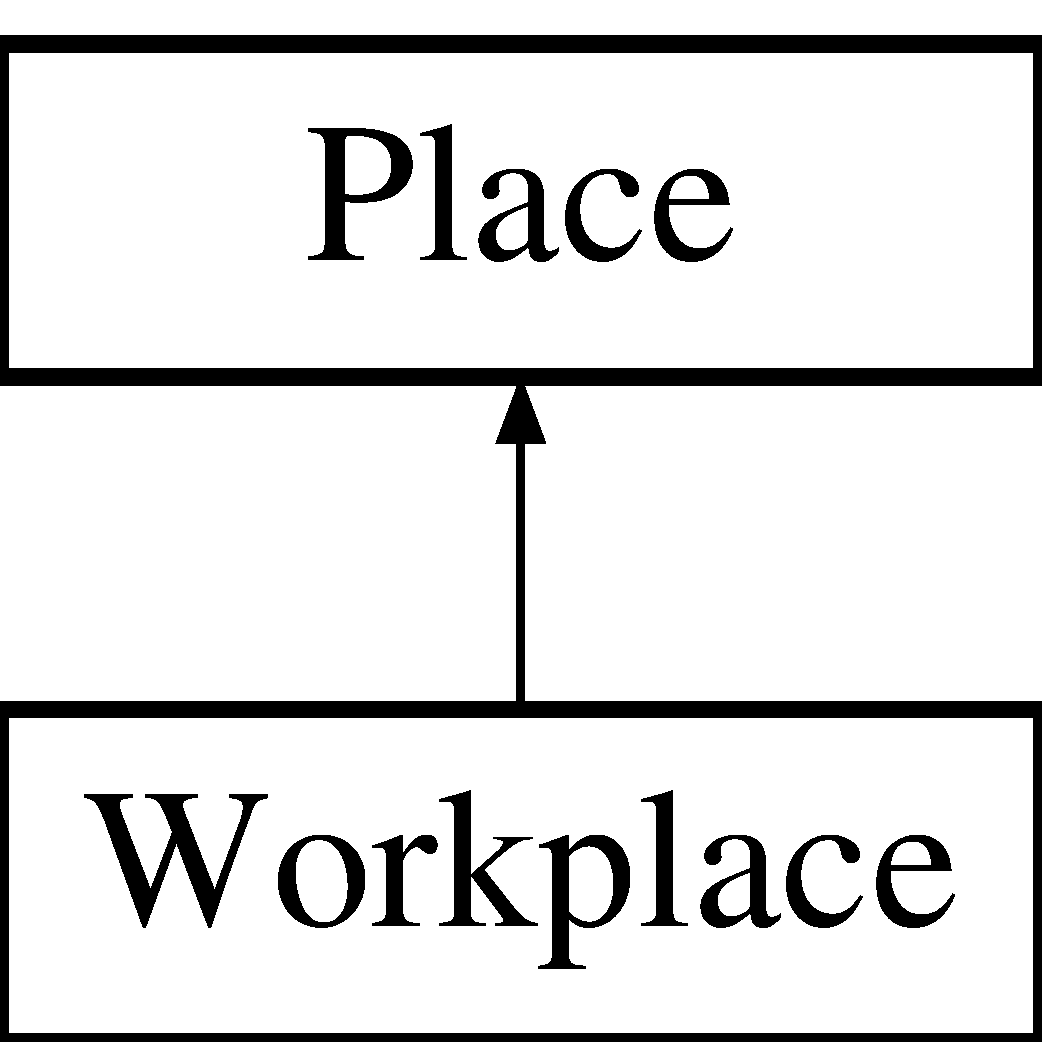
\includegraphics[height=2.000000cm]{classWorkplace}
\end{center}
\end{figure}
\subsection*{Public Member Functions}
\begin{DoxyCompactItemize}
\item 
\hyperlink{classWorkplace_af182fb46622e45e1c45cec7ab5c3a3c1}{Workplace} ()=default
\begin{DoxyCompactList}\small\item\em Creates a \hyperlink{classWorkplace}{Workplace} object with default attributes. \end{DoxyCompactList}\item 
\hyperlink{classWorkplace_a0d116e1103d53e5417c295eebcfc7f39}{Workplace} (const int work\+\_\+\+ID, const double xi, const double yi, const double severity\+\_\+cor, const double psi, const double beta)
\begin{DoxyCompactList}\small\item\em Creates a \hyperlink{classWorkplace}{Workplace} object. \end{DoxyCompactList}\item 
void \hyperlink{classWorkplace_a48ef6cf8af0753240063ea8c00f4cc63}{add\+\_\+symptomatic} (double inf\+\_\+var) override
\begin{DoxyCompactList}\small\item\em Include symptomatic contribution in the sum. \end{DoxyCompactList}\item 
void \hyperlink{classWorkplace_a0d601f969c1403a8c51e1e940a9ed6c8}{change\+\_\+absenteeism\+\_\+correction} (const double val)
\item 
double \hyperlink{classWorkplace_a8ea81599e58cc96e4cf7c1e536e3b9d7}{get\+\_\+absenteeism\+\_\+correction} () const
\item 
void \hyperlink{classWorkplace_af4fcc642e32e174bab45def56b7c6f05}{print\+\_\+basic} (std\+::ostream \&where) const override
\begin{DoxyCompactList}\small\item\em Save information about a \hyperlink{classWorkplace}{Workplace} object. \end{DoxyCompactList}\end{DoxyCompactItemize}
\subsection*{Additional Inherited Members}


\subsection{Constructor \& Destructor Documentation}
\mbox{\Hypertarget{classWorkplace_af182fb46622e45e1c45cec7ab5c3a3c1}\label{classWorkplace_af182fb46622e45e1c45cec7ab5c3a3c1}} 
\index{Workplace@{Workplace}!Workplace@{Workplace}}
\index{Workplace@{Workplace}!Workplace@{Workplace}}
\subsubsection{\texorpdfstring{Workplace()}{Workplace()}\hspace{0.1cm}{\footnotesize\ttfamily [1/2]}}
{\footnotesize\ttfamily Workplace\+::\+Workplace (\begin{DoxyParamCaption}{ }\end{DoxyParamCaption})\hspace{0.3cm}{\ttfamily [default]}}



Creates a \hyperlink{classWorkplace}{Workplace} object with default attributes. 

\mbox{\Hypertarget{classWorkplace_a0d116e1103d53e5417c295eebcfc7f39}\label{classWorkplace_a0d116e1103d53e5417c295eebcfc7f39}} 
\index{Workplace@{Workplace}!Workplace@{Workplace}}
\index{Workplace@{Workplace}!Workplace@{Workplace}}
\subsubsection{\texorpdfstring{Workplace()}{Workplace()}\hspace{0.1cm}{\footnotesize\ttfamily [2/2]}}
{\footnotesize\ttfamily Workplace\+::\+Workplace (\begin{DoxyParamCaption}\item[{const int}]{work\+\_\+\+ID,  }\item[{const double}]{xi,  }\item[{const double}]{yi,  }\item[{const double}]{severity\+\_\+cor,  }\item[{const double}]{psi,  }\item[{const double}]{beta }\end{DoxyParamCaption})\hspace{0.3cm}{\ttfamily [inline]}}



Creates a \hyperlink{classWorkplace}{Workplace} object. 

\hyperlink{classHospital}{Hospital} with custom ID, location, and infection parameters


\begin{DoxyParams}{Parameters}
{\em work\+\_\+\+ID} & -\/ ID of the workplace \\
\hline
{\em xi} & -\/ x coordinate of the workplace \\
\hline
{\em yi} & -\/ y coordinate of the workplace \\
\hline
{\em severity\+\_\+cor} & -\/ severity correction for symptomatic \\
\hline
{\em psi} & -\/ absenteeism correction \\
\hline
{\em beta} & -\/ infection transmission rate, 1/time \\
\hline
\end{DoxyParams}


\subsection{Member Function Documentation}
\mbox{\Hypertarget{classWorkplace_a48ef6cf8af0753240063ea8c00f4cc63}\label{classWorkplace_a48ef6cf8af0753240063ea8c00f4cc63}} 
\index{Workplace@{Workplace}!add\+\_\+symptomatic@{add\+\_\+symptomatic}}
\index{add\+\_\+symptomatic@{add\+\_\+symptomatic}!Workplace@{Workplace}}
\subsubsection{\texorpdfstring{add\+\_\+symptomatic()}{add\_symptomatic()}}
{\footnotesize\ttfamily void Workplace\+::add\+\_\+symptomatic (\begin{DoxyParamCaption}\item[{double}]{inf\+\_\+var }\end{DoxyParamCaption})\hspace{0.3cm}{\ttfamily [inline]}, {\ttfamily [override]}, {\ttfamily [virtual]}}



Include symptomatic contribution in the sum. 


\begin{DoxyParams}{Parameters}
{\em inf\+\_\+var} & -\/ agent infectiousness variability factor \\
\hline
\end{DoxyParams}


Reimplemented from \hyperlink{classPlace_a5216539c8589d41aad430513740fa15c}{Place}.

\mbox{\Hypertarget{classWorkplace_a0d601f969c1403a8c51e1e940a9ed6c8}\label{classWorkplace_a0d601f969c1403a8c51e1e940a9ed6c8}} 
\index{Workplace@{Workplace}!change\+\_\+absenteeism\+\_\+correction@{change\+\_\+absenteeism\+\_\+correction}}
\index{change\+\_\+absenteeism\+\_\+correction@{change\+\_\+absenteeism\+\_\+correction}!Workplace@{Workplace}}
\subsubsection{\texorpdfstring{change\+\_\+absenteeism\+\_\+correction()}{change\_absenteeism\_correction()}}
{\footnotesize\ttfamily void Workplace\+::change\+\_\+absenteeism\+\_\+correction (\begin{DoxyParamCaption}\item[{const double}]{val }\end{DoxyParamCaption})\hspace{0.3cm}{\ttfamily [inline]}}

\mbox{\Hypertarget{classWorkplace_a8ea81599e58cc96e4cf7c1e536e3b9d7}\label{classWorkplace_a8ea81599e58cc96e4cf7c1e536e3b9d7}} 
\index{Workplace@{Workplace}!get\+\_\+absenteeism\+\_\+correction@{get\+\_\+absenteeism\+\_\+correction}}
\index{get\+\_\+absenteeism\+\_\+correction@{get\+\_\+absenteeism\+\_\+correction}!Workplace@{Workplace}}
\subsubsection{\texorpdfstring{get\+\_\+absenteeism\+\_\+correction()}{get\_absenteeism\_correction()}}
{\footnotesize\ttfamily double Workplace\+::get\+\_\+absenteeism\+\_\+correction (\begin{DoxyParamCaption}{ }\end{DoxyParamCaption}) const\hspace{0.3cm}{\ttfamily [inline]}}

\mbox{\Hypertarget{classWorkplace_af4fcc642e32e174bab45def56b7c6f05}\label{classWorkplace_af4fcc642e32e174bab45def56b7c6f05}} 
\index{Workplace@{Workplace}!print\+\_\+basic@{print\+\_\+basic}}
\index{print\+\_\+basic@{print\+\_\+basic}!Workplace@{Workplace}}
\subsubsection{\texorpdfstring{print\+\_\+basic()}{print\_basic()}}
{\footnotesize\ttfamily void Workplace\+::print\+\_\+basic (\begin{DoxyParamCaption}\item[{std\+::ostream \&}]{where }\end{DoxyParamCaption}) const\hspace{0.3cm}{\ttfamily [override]}, {\ttfamily [virtual]}}



Save information about a \hyperlink{classWorkplace}{Workplace} object. 

Saves to a file, everything but detailed agent information; order is ID $\vert$ x $\vert$ y $\vert$ number of agents $\vert$ number of infected agents $\vert$ ck $\vert$ beta\+\_\+j $\vert$ psi\+\_\+j Delimiter is a space. 
\begin{DoxyParams}{Parameters}
{\em where} & -\/ output stream \\
\hline
\end{DoxyParams}


Reimplemented from \hyperlink{classPlace_a9aa7649e0b91c5f61a5f71e9ca808fe1}{Place}.



The documentation for this class was generated from the following files\+:\begin{DoxyCompactItemize}
\item 
include/places/\hyperlink{workplace_8h}{workplace.\+h}\item 
src/places/\hyperlink{workplace_8cpp}{workplace.\+cpp}\end{DoxyCompactItemize}

\chapter{File Documentation}
\hypertarget{abm_8h}{}\section{include/abm.h File Reference}
\label{abm_8h}\index{include/abm.\+h@{include/abm.\+h}}
{\ttfamily \#include \char`\"{}abm\+\_\+include.\+h\char`\"{}}\newline
\subsection*{Classes}
\begin{DoxyCompactItemize}
\item 
class \hyperlink{classABM}{A\+BM}
\end{DoxyCompactItemize}

\hypertarget{abm__include_8h}{}\section{include/abm\+\_\+include.h File Reference}
\label{abm__include_8h}\index{include/abm\+\_\+include.\+h@{include/abm\+\_\+include.\+h}}
{\ttfamily \#include \char`\"{}places/place.\+h\char`\"{}}\newline
{\ttfamily \#include \char`\"{}places/household.\+h\char`\"{}}\newline
{\ttfamily \#include \char`\"{}places/retirement\+\_\+home.\+h\char`\"{}}\newline
{\ttfamily \#include \char`\"{}places/school.\+h\char`\"{}}\newline
{\ttfamily \#include \char`\"{}places/workplace.\+h\char`\"{}}\newline
{\ttfamily \#include \char`\"{}places/hospital.\+h\char`\"{}}\newline
{\ttfamily \#include \char`\"{}transitions/transitions.\+h\char`\"{}}\newline
{\ttfamily \#include \char`\"{}states\+\_\+manager/states\+\_\+manager.\+h\char`\"{}}\newline
{\ttfamily \#include \char`\"{}common.\+h\char`\"{}}\newline
{\ttfamily \#include \char`\"{}./io\+\_\+operations/abm\+\_\+io.\+h\char`\"{}}\newline
{\ttfamily \#include \char`\"{}./io\+\_\+operations/load\+\_\+parameters.\+h\char`\"{}}\newline
{\ttfamily \#include \char`\"{}agent.\+h\char`\"{}}\newline
{\ttfamily \#include \char`\"{}infection.\+h\char`\"{}}\newline
{\ttfamily \#include \char`\"{}testing.\+h\char`\"{}}\newline
{\ttfamily \#include \char`\"{}contributions.\+h\char`\"{}}\newline
{\ttfamily \#include \char`\"{}flu.\+h\char`\"{}}\newline
{\ttfamily \#include \char`\"{}utils.\+h\char`\"{}}\newline

\hypertarget{agent_8h}{}\section{include/agent.h File Reference}
\label{agent_8h}\index{include/agent.\+h@{include/agent.\+h}}
{\ttfamily \#include \char`\"{}common.\+h\char`\"{}}\newline
{\ttfamily \#include \char`\"{}infection.\+h\char`\"{}}\newline
\subsection*{Classes}
\begin{DoxyCompactItemize}
\item 
class \hyperlink{classAgent}{Agent}
\end{DoxyCompactItemize}
\subsection*{Functions}
\begin{DoxyCompactItemize}
\item 
std\+::ostream \& \hyperlink{agent_8h_ad9bcccf2df99d6fe282048ff28773728}{operator$<$$<$} (std\+::ostream \&out, const \hyperlink{classAgent}{Agent} \&agent)
\begin{DoxyCompactList}\small\item\em Overloaded ostream operator for I/O. \end{DoxyCompactList}\end{DoxyCompactItemize}


\subsection{Function Documentation}
\mbox{\Hypertarget{agent_8h_ad9bcccf2df99d6fe282048ff28773728}\label{agent_8h_ad9bcccf2df99d6fe282048ff28773728}} 
\index{agent.\+h@{agent.\+h}!operator$<$$<$@{operator$<$$<$}}
\index{operator$<$$<$@{operator$<$$<$}!agent.\+h@{agent.\+h}}
\subsubsection{\texorpdfstring{operator$<$$<$()}{operator<<()}}
{\footnotesize\ttfamily std\+::ostream\& operator$<$$<$ (\begin{DoxyParamCaption}\item[{std\+::ostream \&}]{out,  }\item[{const \hyperlink{classAgent}{Agent} \&}]{agent }\end{DoxyParamCaption})}



Overloaded ostream operator for I/O. 


\hypertarget{common_8h}{}\section{include/common.h File Reference}
\label{common_8h}\index{include/common.\+h@{include/common.\+h}}
{\ttfamily \#include $<$iostream$>$}\newline
{\ttfamily \#include $<$fstream$>$}\newline
{\ttfamily \#include $<$sstream$>$}\newline
{\ttfamily \#include $<$iterator$>$}\newline
{\ttfamily \#include $<$cstring$>$}\newline
{\ttfamily \#include $<$stdexcept$>$}\newline
{\ttfamily \#include $<$cmath$>$}\newline
{\ttfamily \#include $<$random$>$}\newline
{\ttfamily \#include $<$algorithm$>$}\newline
{\ttfamily \#include $<$string$>$}\newline
{\ttfamily \#include $<$vector$>$}\newline
{\ttfamily \#include $<$cctype$>$}\newline
{\ttfamily \#include $<$map$>$}\newline

\hypertarget{contributions_8h}{}\section{include/contributions.h File Reference}
\label{contributions_8h}\index{include/contributions.\+h@{include/contributions.\+h}}
{\ttfamily \#include \char`\"{}places/place.\+h\char`\"{}}\newline
{\ttfamily \#include \char`\"{}places/household.\+h\char`\"{}}\newline
{\ttfamily \#include \char`\"{}places/retirement\+\_\+home.\+h\char`\"{}}\newline
{\ttfamily \#include \char`\"{}places/school.\+h\char`\"{}}\newline
{\ttfamily \#include \char`\"{}places/workplace.\+h\char`\"{}}\newline
{\ttfamily \#include \char`\"{}places/hospital.\+h\char`\"{}}\newline
{\ttfamily \#include \char`\"{}common.\+h\char`\"{}}\newline
{\ttfamily \#include \char`\"{}agent.\+h\char`\"{}}\newline
{\ttfamily \#include \char`\"{}flu.\+h\char`\"{}}\newline
\subsection*{Classes}
\begin{DoxyCompactItemize}
\item 
class \hyperlink{classContributions}{Contributions}
\end{DoxyCompactItemize}

\hypertarget{flu_8h}{}\section{include/flu.h File Reference}
\label{flu_8h}\index{include/flu.\+h@{include/flu.\+h}}
{\ttfamily \#include \char`\"{}common.\+h\char`\"{}}\newline
{\ttfamily \#include \char`\"{}testing.\+h\char`\"{}}\newline
{\ttfamily \#include \char`\"{}rng.\+h\char`\"{}}\newline
\subsection*{Classes}
\begin{DoxyCompactItemize}
\item 
class \hyperlink{classFlu}{Flu}
\end{DoxyCompactItemize}

\hypertarget{infection_8h}{}\section{include/infection.h File Reference}
\label{infection_8h}\index{include/infection.\+h@{include/infection.\+h}}
{\ttfamily \#include \char`\"{}common.\+h\char`\"{}}\newline
{\ttfamily \#include \char`\"{}rng.\+h\char`\"{}}\newline
{\ttfamily \#include \char`\"{}utils.\+h\char`\"{}}\newline
{\ttfamily \#include $<$tuple$>$}\newline
\subsection*{Classes}
\begin{DoxyCompactItemize}
\item 
class \hyperlink{classInfection}{Infection}
\end{DoxyCompactItemize}
\subsection*{Functions}
\begin{DoxyCompactItemize}
\item 
std\+::ostream \& \hyperlink{infection_8h_a6fbe68152f27600074f425b4c462312d}{operator$<$$<$} (std\+::ostream \&out, const \hyperlink{classInfection}{Infection} \&infection)
\begin{DoxyCompactList}\small\item\em Overloaded ostream operator for I/O. \end{DoxyCompactList}\end{DoxyCompactItemize}


\subsection{Function Documentation}
\mbox{\Hypertarget{infection_8h_a6fbe68152f27600074f425b4c462312d}\label{infection_8h_a6fbe68152f27600074f425b4c462312d}} 
\index{infection.\+h@{infection.\+h}!operator$<$$<$@{operator$<$$<$}}
\index{operator$<$$<$@{operator$<$$<$}!infection.\+h@{infection.\+h}}
\subsubsection{\texorpdfstring{operator$<$$<$()}{operator<<()}}
{\footnotesize\ttfamily std\+::ostream\& operator$<$$<$ (\begin{DoxyParamCaption}\item[{std\+::ostream \&}]{out,  }\item[{const \hyperlink{classInfection}{Infection} \&}]{infection }\end{DoxyParamCaption})}



Overloaded ostream operator for I/O. 


\hypertarget{abm__io_8h}{}\section{include/io\+\_\+operations/abm\+\_\+io.h File Reference}
\label{abm__io_8h}\index{include/io\+\_\+operations/abm\+\_\+io.\+h@{include/io\+\_\+operations/abm\+\_\+io.\+h}}
{\ttfamily \#include \char`\"{}File\+Handler.\+h\char`\"{}}\newline
{\ttfamily \#include \char`\"{}../common.\+h\char`\"{}}\newline
\subsection*{Classes}
\begin{DoxyCompactItemize}
\item 
class \hyperlink{classAbmIO}{Abm\+IO}
\end{DoxyCompactItemize}

\hypertarget{FileHandler_8h}{}\section{include/io\+\_\+operations/\+File\+Handler.h File Reference}
\label{FileHandler_8h}\index{include/io\+\_\+operations/\+File\+Handler.\+h@{include/io\+\_\+operations/\+File\+Handler.\+h}}
{\ttfamily \#include \char`\"{}../common.\+h\char`\"{}}\newline
{\ttfamily \#include $<$ios$>$}\newline
\subsection*{Classes}
\begin{DoxyCompactItemize}
\item 
class \hyperlink{classFileHandler}{File\+Handler}
\end{DoxyCompactItemize}

\hypertarget{load__parameters_8h}{}\section{include/io\+\_\+operations/load\+\_\+parameters.h File Reference}
\label{load__parameters_8h}\index{include/io\+\_\+operations/load\+\_\+parameters.\+h@{include/io\+\_\+operations/load\+\_\+parameters.\+h}}
{\ttfamily \#include \char`\"{}File\+Handler.\+h\char`\"{}}\newline
{\ttfamily \#include \char`\"{}../common.\+h\char`\"{}}\newline
\subsection*{Classes}
\begin{DoxyCompactItemize}
\item 
class \hyperlink{classLoadParameters}{Load\+Parameters}
\end{DoxyCompactItemize}

\hypertarget{hospital_8h}{}\section{include/places/hospital.h File Reference}
\label{hospital_8h}\index{include/places/hospital.\+h@{include/places/hospital.\+h}}
{\ttfamily \#include \char`\"{}place.\+h\char`\"{}}\newline
\subsection*{Classes}
\begin{DoxyCompactItemize}
\item 
class \hyperlink{classHospital}{Hospital}
\end{DoxyCompactItemize}

\hypertarget{household_8h}{}\section{include/places/household.h File Reference}
\label{household_8h}\index{include/places/household.\+h@{include/places/household.\+h}}
{\ttfamily \#include \char`\"{}place.\+h\char`\"{}}\newline
{\ttfamily \#include \char`\"{}../infection.\+h\char`\"{}}\newline
\subsection*{Classes}
\begin{DoxyCompactItemize}
\item 
class \hyperlink{classHousehold}{Household}
\end{DoxyCompactItemize}

\hypertarget{place_8h}{}\section{include/places/place.h File Reference}
\label{place_8h}\index{include/places/place.\+h@{include/places/place.\+h}}
{\ttfamily \#include \char`\"{}../common.\+h\char`\"{}}\newline
\subsection*{Classes}
\begin{DoxyCompactItemize}
\item 
class \hyperlink{classPlace}{Place}
\end{DoxyCompactItemize}
\subsection*{Functions}
\begin{DoxyCompactItemize}
\item 
std\+::ostream \& \hyperlink{place_8h_a1bfd2e5f445a9e1bc833698fd39d3606}{operator$<$$<$} (std\+::ostream \&out, const \hyperlink{classPlace}{Place} \&place)
\begin{DoxyCompactList}\small\item\em Overloaded ostream operator for I/O. \end{DoxyCompactList}\end{DoxyCompactItemize}


\subsection{Function Documentation}
\mbox{\Hypertarget{place_8h_a1bfd2e5f445a9e1bc833698fd39d3606}\label{place_8h_a1bfd2e5f445a9e1bc833698fd39d3606}} 
\index{place.\+h@{place.\+h}!operator$<$$<$@{operator$<$$<$}}
\index{operator$<$$<$@{operator$<$$<$}!place.\+h@{place.\+h}}
\subsubsection{\texorpdfstring{operator$<$$<$()}{operator<<()}}
{\footnotesize\ttfamily std\+::ostream\& operator$<$$<$ (\begin{DoxyParamCaption}\item[{std\+::ostream \&}]{out,  }\item[{const \hyperlink{classPlace}{Place} \&}]{place }\end{DoxyParamCaption})}



Overloaded ostream operator for I/O. 


\hypertarget{retirement__home_8h}{}\section{include/places/retirement\+\_\+home.h File Reference}
\label{retirement__home_8h}\index{include/places/retirement\+\_\+home.\+h@{include/places/retirement\+\_\+home.\+h}}
{\ttfamily \#include \char`\"{}place.\+h\char`\"{}}\newline
\subsection*{Classes}
\begin{DoxyCompactItemize}
\item 
class \hyperlink{classRetirementHome}{Retirement\+Home}
\end{DoxyCompactItemize}

\hypertarget{school_8h}{}\section{include/places/school.h File Reference}
\label{school_8h}\index{include/places/school.\+h@{include/places/school.\+h}}
{\ttfamily \#include \char`\"{}place.\+h\char`\"{}}\newline
\subsection*{Classes}
\begin{DoxyCompactItemize}
\item 
class \hyperlink{classSchool}{School}
\end{DoxyCompactItemize}

\hypertarget{workplace_8h}{}\section{include/places/workplace.h File Reference}
\label{workplace_8h}\index{include/places/workplace.\+h@{include/places/workplace.\+h}}
{\ttfamily \#include \char`\"{}place.\+h\char`\"{}}\newline
\subsection*{Classes}
\begin{DoxyCompactItemize}
\item 
class \hyperlink{classWorkplace}{Workplace}
\end{DoxyCompactItemize}

\hypertarget{rng_8h}{}\section{include/rng.h File Reference}
\label{rng_8h}\index{include/rng.\+h@{include/rng.\+h}}
{\ttfamily \#include $<$random$>$}\newline
\subsection*{Classes}
\begin{DoxyCompactItemize}
\item 
class \hyperlink{classRNG}{R\+NG}
\end{DoxyCompactItemize}

\hypertarget{hsp__employee__states__manager_8h}{}\section{include/states\+\_\+manager/hsp\+\_\+employee\+\_\+states\+\_\+manager.h File Reference}
\label{hsp__employee__states__manager_8h}\index{include/states\+\_\+manager/hsp\+\_\+employee\+\_\+states\+\_\+manager.\+h@{include/states\+\_\+manager/hsp\+\_\+employee\+\_\+states\+\_\+manager.\+h}}
{\ttfamily \#include \char`\"{}../common.\+h\char`\"{}}\newline
{\ttfamily \#include \char`\"{}../io\+\_\+operations/abm\+\_\+io.\+h\char`\"{}}\newline
{\ttfamily \#include \char`\"{}../agent.\+h\char`\"{}}\newline
\subsection*{Classes}
\begin{DoxyCompactItemize}
\item 
class \hyperlink{classHspEmployeeStatesManager}{Hsp\+Employee\+States\+Manager}
\end{DoxyCompactItemize}

\hypertarget{regular__states__manager_8h}{}\section{include/states\+\_\+manager/regular\+\_\+states\+\_\+manager.h File Reference}
\label{regular__states__manager_8h}\index{include/states\+\_\+manager/regular\+\_\+states\+\_\+manager.\+h@{include/states\+\_\+manager/regular\+\_\+states\+\_\+manager.\+h}}
{\ttfamily \#include \char`\"{}../common.\+h\char`\"{}}\newline
{\ttfamily \#include \char`\"{}../io\+\_\+operations/abm\+\_\+io.\+h\char`\"{}}\newline
{\ttfamily \#include \char`\"{}../agent.\+h\char`\"{}}\newline
\subsection*{Classes}
\begin{DoxyCompactItemize}
\item 
class \hyperlink{classRegularStatesManager}{Regular\+States\+Manager}
\end{DoxyCompactItemize}

\hypertarget{states__manager_8h}{}\section{include/states\+\_\+manager/states\+\_\+manager.h File Reference}
\label{states__manager_8h}\index{include/states\+\_\+manager/states\+\_\+manager.\+h@{include/states\+\_\+manager/states\+\_\+manager.\+h}}
{\ttfamily \#include \char`\"{}../common.\+h\char`\"{}}\newline
{\ttfamily \#include \char`\"{}../io\+\_\+operations/abm\+\_\+io.\+h\char`\"{}}\newline
{\ttfamily \#include \char`\"{}../agent.\+h\char`\"{}}\newline
\subsection*{Classes}
\begin{DoxyCompactItemize}
\item 
class \hyperlink{classStatesManager}{States\+Manager}
\end{DoxyCompactItemize}

\hypertarget{testing_8h}{}\section{include/testing.h File Reference}
\label{testing_8h}\index{include/testing.\+h@{include/testing.\+h}}
{\ttfamily \#include \char`\"{}common.\+h\char`\"{}}\newline
{\ttfamily \#include \char`\"{}utils.\+h\char`\"{}}\newline
{\ttfamily \#include $<$deque$>$}\newline
\subsection*{Classes}
\begin{DoxyCompactItemize}
\item 
class \hyperlink{classTesting}{Testing}
\end{DoxyCompactItemize}

\hypertarget{flu__transitions_8h}{}\section{include/transitions/flu\+\_\+transitions.h File Reference}
\label{flu__transitions_8h}\index{include/transitions/flu\+\_\+transitions.\+h@{include/transitions/flu\+\_\+transitions.\+h}}
{\ttfamily \#include \char`\"{}../places/place.\+h\char`\"{}}\newline
{\ttfamily \#include \char`\"{}../places/household.\+h\char`\"{}}\newline
{\ttfamily \#include \char`\"{}../places/school.\+h\char`\"{}}\newline
{\ttfamily \#include \char`\"{}../places/workplace.\+h\char`\"{}}\newline
{\ttfamily \#include \char`\"{}../places/hospital.\+h\char`\"{}}\newline
{\ttfamily \#include \char`\"{}../places/retirement\+\_\+home.\+h\char`\"{}}\newline
{\ttfamily \#include \char`\"{}../common.\+h\char`\"{}}\newline
{\ttfamily \#include \char`\"{}../agent.\+h\char`\"{}}\newline
{\ttfamily \#include \char`\"{}../infection.\+h\char`\"{}}\newline
{\ttfamily \#include \char`\"{}../states\+\_\+manager/regular\+\_\+states\+\_\+manager.\+h\char`\"{}}\newline
{\ttfamily \#include \char`\"{}../flu.\+h\char`\"{}}\newline
{\ttfamily \#include \char`\"{}../testing.\+h\char`\"{}}\newline
\subsection*{Classes}
\begin{DoxyCompactItemize}
\item 
class \hyperlink{classFluTransitions}{Flu\+Transitions}
\end{DoxyCompactItemize}

\hypertarget{hsp__employee__transitions_8h}{}\section{include/transitions/hsp\+\_\+employee\+\_\+transitions.h File Reference}
\label{hsp__employee__transitions_8h}\index{include/transitions/hsp\+\_\+employee\+\_\+transitions.\+h@{include/transitions/hsp\+\_\+employee\+\_\+transitions.\+h}}
{\ttfamily \#include \char`\"{}../places/place.\+h\char`\"{}}\newline
{\ttfamily \#include \char`\"{}../places/household.\+h\char`\"{}}\newline
{\ttfamily \#include \char`\"{}../places/school.\+h\char`\"{}}\newline
{\ttfamily \#include \char`\"{}../places/workplace.\+h\char`\"{}}\newline
{\ttfamily \#include \char`\"{}../places/hospital.\+h\char`\"{}}\newline
{\ttfamily \#include \char`\"{}../common.\+h\char`\"{}}\newline
{\ttfamily \#include \char`\"{}../agent.\+h\char`\"{}}\newline
{\ttfamily \#include \char`\"{}../infection.\+h\char`\"{}}\newline
{\ttfamily \#include \char`\"{}../states\+\_\+manager/hsp\+\_\+employee\+\_\+states\+\_\+manager.\+h\char`\"{}}\newline
{\ttfamily \#include \char`\"{}../flu.\+h\char`\"{}}\newline
{\ttfamily \#include \char`\"{}../testing.\+h\char`\"{}}\newline
\subsection*{Classes}
\begin{DoxyCompactItemize}
\item 
class \hyperlink{classHspEmployeeTransitions}{Hsp\+Employee\+Transitions}
\end{DoxyCompactItemize}

\hypertarget{hsp__patient__transitions_8h}{}\section{include/transitions/hsp\+\_\+patient\+\_\+transitions.h File Reference}
\label{hsp__patient__transitions_8h}\index{include/transitions/hsp\+\_\+patient\+\_\+transitions.\+h@{include/transitions/hsp\+\_\+patient\+\_\+transitions.\+h}}
{\ttfamily \#include \char`\"{}../places/place.\+h\char`\"{}}\newline
{\ttfamily \#include \char`\"{}../places/household.\+h\char`\"{}}\newline
{\ttfamily \#include \char`\"{}../places/school.\+h\char`\"{}}\newline
{\ttfamily \#include \char`\"{}../places/workplace.\+h\char`\"{}}\newline
{\ttfamily \#include \char`\"{}../places/hospital.\+h\char`\"{}}\newline
{\ttfamily \#include \char`\"{}../common.\+h\char`\"{}}\newline
{\ttfamily \#include \char`\"{}../agent.\+h\char`\"{}}\newline
{\ttfamily \#include \char`\"{}../infection.\+h\char`\"{}}\newline
{\ttfamily \#include \char`\"{}../states\+\_\+manager/hsp\+\_\+employee\+\_\+states\+\_\+manager.\+h\char`\"{}}\newline
{\ttfamily \#include \char`\"{}../flu.\+h\char`\"{}}\newline
\subsection*{Classes}
\begin{DoxyCompactItemize}
\item 
class \hyperlink{classHspPatientTransitions}{Hsp\+Patient\+Transitions}
\end{DoxyCompactItemize}

\hypertarget{regular__transitions_8h}{}\section{include/transitions/regular\+\_\+transitions.h File Reference}
\label{regular__transitions_8h}\index{include/transitions/regular\+\_\+transitions.\+h@{include/transitions/regular\+\_\+transitions.\+h}}
{\ttfamily \#include \char`\"{}../places/place.\+h\char`\"{}}\newline
{\ttfamily \#include \char`\"{}../places/household.\+h\char`\"{}}\newline
{\ttfamily \#include \char`\"{}../places/school.\+h\char`\"{}}\newline
{\ttfamily \#include \char`\"{}../places/workplace.\+h\char`\"{}}\newline
{\ttfamily \#include \char`\"{}../places/hospital.\+h\char`\"{}}\newline
{\ttfamily \#include \char`\"{}../places/retirement\+\_\+home.\+h\char`\"{}}\newline
{\ttfamily \#include \char`\"{}../common.\+h\char`\"{}}\newline
{\ttfamily \#include \char`\"{}../agent.\+h\char`\"{}}\newline
{\ttfamily \#include \char`\"{}../infection.\+h\char`\"{}}\newline
{\ttfamily \#include \char`\"{}../states\+\_\+manager/regular\+\_\+states\+\_\+manager.\+h\char`\"{}}\newline
{\ttfamily \#include \char`\"{}../flu.\+h\char`\"{}}\newline
{\ttfamily \#include \char`\"{}../testing.\+h\char`\"{}}\newline
\subsection*{Classes}
\begin{DoxyCompactItemize}
\item 
class \hyperlink{classRegularTransitions}{Regular\+Transitions}
\end{DoxyCompactItemize}

\hypertarget{transitions_8h}{}\section{include/transitions/transitions.h File Reference}
\label{transitions_8h}\index{include/transitions/transitions.\+h@{include/transitions/transitions.\+h}}
{\ttfamily \#include \char`\"{}../places/place.\+h\char`\"{}}\newline
{\ttfamily \#include \char`\"{}../places/household.\+h\char`\"{}}\newline
{\ttfamily \#include \char`\"{}../places/school.\+h\char`\"{}}\newline
{\ttfamily \#include \char`\"{}../places/workplace.\+h\char`\"{}}\newline
{\ttfamily \#include \char`\"{}../places/hospital.\+h\char`\"{}}\newline
{\ttfamily \#include \char`\"{}../places/retirement\+\_\+home.\+h\char`\"{}}\newline
{\ttfamily \#include \char`\"{}regular\+\_\+transitions.\+h\char`\"{}}\newline
{\ttfamily \#include \char`\"{}hsp\+\_\+employee\+\_\+transitions.\+h\char`\"{}}\newline
{\ttfamily \#include \char`\"{}hsp\+\_\+patient\+\_\+transitions.\+h\char`\"{}}\newline
{\ttfamily \#include \char`\"{}flu\+\_\+transitions.\+h\char`\"{}}\newline
{\ttfamily \#include \char`\"{}../common.\+h\char`\"{}}\newline
{\ttfamily \#include \char`\"{}../agent.\+h\char`\"{}}\newline
{\ttfamily \#include \char`\"{}../infection.\+h\char`\"{}}\newline
{\ttfamily \#include \char`\"{}../flu.\+h\char`\"{}}\newline
{\ttfamily \#include \char`\"{}../testing.\+h\char`\"{}}\newline
\subsection*{Classes}
\begin{DoxyCompactItemize}
\item 
class \hyperlink{classTransitions}{Transitions}
\end{DoxyCompactItemize}

\hypertarget{utils_8h}{}\section{include/utils.h File Reference}
\label{utils_8h}\index{include/utils.\+h@{include/utils.\+h}}
{\ttfamily \#include \char`\"{}common.\+h\char`\"{}}\newline
\subsection*{Functions}
\begin{DoxyCompactItemize}
\item 
std\+::string \hyperlink{utils_8h_a3dc8e1f0b48dced7ac485497d3b04ced}{str\+\_\+to\+\_\+lower} (std\+::string s)
\begin{DoxyCompactList}\small\item\em Convert a string to all lower case. \end{DoxyCompactList}\item 
{\footnotesize template$<$typename T $>$ }\\bool \hyperlink{utils_8h_a38660b404ed851d15fc3ce865fa47311}{equal\+\_\+floats} (T, T, T)
\begin{DoxyCompactList}\small\item\em Compare num1 and num2 as inexact values. \end{DoxyCompactList}\end{DoxyCompactItemize}


\subsection{Function Documentation}
\mbox{\Hypertarget{utils_8h_a38660b404ed851d15fc3ce865fa47311}\label{utils_8h_a38660b404ed851d15fc3ce865fa47311}} 
\index{utils.\+h@{utils.\+h}!equal\+\_\+floats@{equal\+\_\+floats}}
\index{equal\+\_\+floats@{equal\+\_\+floats}!utils.\+h@{utils.\+h}}
\subsubsection{\texorpdfstring{equal\+\_\+floats()}{equal\_floats()}}
{\footnotesize\ttfamily template$<$typename T $>$ \\
bool equal\+\_\+floats (\begin{DoxyParamCaption}\item[{T}]{num1,  }\item[{T}]{num2,  }\item[{T}]{tol }\end{DoxyParamCaption})}



Compare num1 and num2 as inexact values. 

For floating point compoarisons, i.\+e. floats, doubles Current version based on \href{https://stackoverflow.com/a/15012792/2763915}{\tt https\+://stackoverflow.\+com/a/15012792/2763915} 
\begin{DoxyParams}{Parameters}
{\em num1} & -\/ first number \\
\hline
{\em num2} & -\/ second number \\
\hline
{\em tol} & -\/ relative tolerance for comparison \\
\hline
\end{DoxyParams}
\begin{DoxyReturn}{Returns}
true if equal within the tolerance 
\end{DoxyReturn}
\mbox{\Hypertarget{utils_8h_a3dc8e1f0b48dced7ac485497d3b04ced}\label{utils_8h_a3dc8e1f0b48dced7ac485497d3b04ced}} 
\index{utils.\+h@{utils.\+h}!str\+\_\+to\+\_\+lower@{str\+\_\+to\+\_\+lower}}
\index{str\+\_\+to\+\_\+lower@{str\+\_\+to\+\_\+lower}!utils.\+h@{utils.\+h}}
\subsubsection{\texorpdfstring{str\+\_\+to\+\_\+lower()}{str\_to\_lower()}}
{\footnotesize\ttfamily std\+::string str\+\_\+to\+\_\+lower (\begin{DoxyParamCaption}\item[{std\+::string}]{s }\end{DoxyParamCaption})}



Convert a string to all lower case. 

From \href{https://en.cppreference.com/w/cpp/string/byte/tolower}{\tt https\+://en.\+cppreference.\+com/w/cpp/string/byte/tolower}


\begin{DoxyParams}[1]{Parameters}
\mbox{\tt in}  & {\em s} & -\/ string which will be converted to all lower case \\
\hline
\end{DoxyParams}

\hypertarget{abm_8cpp}{}\section{src/abm.cpp File Reference}
\label{abm_8cpp}\index{src/abm.\+cpp@{src/abm.\+cpp}}
{\ttfamily \#include \char`\"{}../include/abm.\+h\char`\"{}}\newline

\hypertarget{agent_8cpp}{}\section{src/agent.cpp File Reference}
\label{agent_8cpp}\index{src/agent.\+cpp@{src/agent.\+cpp}}
{\ttfamily \#include \char`\"{}../include/agent.\+h\char`\"{}}\newline
\subsection*{Functions}
\begin{DoxyCompactItemize}
\item 
std\+::ostream \& \hyperlink{agent_8cpp_ad9bcccf2df99d6fe282048ff28773728}{operator$<$$<$} (std\+::ostream \&out, const \hyperlink{classAgent}{Agent} \&agent)
\begin{DoxyCompactList}\small\item\em Overloaded ostream operator for I/O. \end{DoxyCompactList}\end{DoxyCompactItemize}


\subsection{Function Documentation}
\mbox{\Hypertarget{agent_8cpp_ad9bcccf2df99d6fe282048ff28773728}\label{agent_8cpp_ad9bcccf2df99d6fe282048ff28773728}} 
\index{agent.\+cpp@{agent.\+cpp}!operator$<$$<$@{operator$<$$<$}}
\index{operator$<$$<$@{operator$<$$<$}!agent.\+cpp@{agent.\+cpp}}
\subsubsection{\texorpdfstring{operator$<$$<$()}{operator<<()}}
{\footnotesize\ttfamily std\+::ostream\& operator$<$$<$ (\begin{DoxyParamCaption}\item[{std\+::ostream \&}]{out,  }\item[{const \hyperlink{classAgent}{Agent} \&}]{agent }\end{DoxyParamCaption})}



Overloaded ostream operator for I/O. 


\hypertarget{contributions_8cpp}{}\section{src/contributions.cpp File Reference}
\label{contributions_8cpp}\index{src/contributions.\+cpp@{src/contributions.\+cpp}}
{\ttfamily \#include \char`\"{}../include/contributions.\+h\char`\"{}}\newline

\hypertarget{flu_8cpp}{}\section{src/flu.cpp File Reference}
\label{flu_8cpp}\index{src/flu.\+cpp@{src/flu.\+cpp}}
{\ttfamily \#include \char`\"{}../include/flu.\+h\char`\"{}}\newline

\hypertarget{infection_8cpp}{}\section{src/infection.cpp File Reference}
\label{infection_8cpp}\index{src/infection.\+cpp@{src/infection.\+cpp}}
{\ttfamily \#include \char`\"{}../include/infection.\+h\char`\"{}}\newline
\subsection*{Functions}
\begin{DoxyCompactItemize}
\item 
std\+::ostream \& \hyperlink{infection_8cpp_a6fbe68152f27600074f425b4c462312d}{operator$<$$<$} (std\+::ostream \&out, const \hyperlink{classInfection}{Infection} \&infection)
\begin{DoxyCompactList}\small\item\em Overloaded ostream operator for I/O. \end{DoxyCompactList}\end{DoxyCompactItemize}


\subsection{Function Documentation}
\mbox{\Hypertarget{infection_8cpp_a6fbe68152f27600074f425b4c462312d}\label{infection_8cpp_a6fbe68152f27600074f425b4c462312d}} 
\index{infection.\+cpp@{infection.\+cpp}!operator$<$$<$@{operator$<$$<$}}
\index{operator$<$$<$@{operator$<$$<$}!infection.\+cpp@{infection.\+cpp}}
\subsubsection{\texorpdfstring{operator$<$$<$()}{operator<<()}}
{\footnotesize\ttfamily std\+::ostream\& operator$<$$<$ (\begin{DoxyParamCaption}\item[{std\+::ostream \&}]{out,  }\item[{const \hyperlink{classInfection}{Infection} \&}]{infection }\end{DoxyParamCaption})}



Overloaded ostream operator for I/O. 


\hypertarget{FileHandler_8cpp}{}\section{src/io\+\_\+operations/\+File\+Handler.cpp File Reference}
\label{FileHandler_8cpp}\index{src/io\+\_\+operations/\+File\+Handler.\+cpp@{src/io\+\_\+operations/\+File\+Handler.\+cpp}}
{\ttfamily \#include \char`\"{}../../include/io\+\_\+operations/\+File\+Handler.\+h\char`\"{}}\newline

\hypertarget{load__parameters_8cpp}{}\section{src/io\+\_\+operations/load\+\_\+parameters.cpp File Reference}
\label{load__parameters_8cpp}\index{src/io\+\_\+operations/load\+\_\+parameters.\+cpp@{src/io\+\_\+operations/load\+\_\+parameters.\+cpp}}
{\ttfamily \#include \char`\"{}../../include/io\+\_\+operations/load\+\_\+parameters.\+h\char`\"{}}\newline

\hypertarget{hospital_8cpp}{}\section{src/places/hospital.cpp File Reference}
\label{hospital_8cpp}\index{src/places/hospital.\+cpp@{src/places/hospital.\+cpp}}
{\ttfamily \#include \char`\"{}../../include/places/hospital.\+h\char`\"{}}\newline

\hypertarget{household_8cpp}{}\section{src/places/household.cpp File Reference}
\label{household_8cpp}\index{src/places/household.\+cpp@{src/places/household.\+cpp}}
{\ttfamily \#include \char`\"{}../../include/places/household.\+h\char`\"{}}\newline

\hypertarget{place_8cpp}{}\section{src/places/place.cpp File Reference}
\label{place_8cpp}\index{src/places/place.\+cpp@{src/places/place.\+cpp}}
{\ttfamily \#include \char`\"{}../../include/places/place.\+h\char`\"{}}\newline
\subsection*{Functions}
\begin{DoxyCompactItemize}
\item 
std\+::ostream \& \hyperlink{place_8cpp_a1bfd2e5f445a9e1bc833698fd39d3606}{operator$<$$<$} (std\+::ostream \&out, const \hyperlink{classPlace}{Place} \&place)
\begin{DoxyCompactList}\small\item\em Overloaded ostream operator for I/O. \end{DoxyCompactList}\end{DoxyCompactItemize}


\subsection{Function Documentation}
\mbox{\Hypertarget{place_8cpp_a1bfd2e5f445a9e1bc833698fd39d3606}\label{place_8cpp_a1bfd2e5f445a9e1bc833698fd39d3606}} 
\index{place.\+cpp@{place.\+cpp}!operator$<$$<$@{operator$<$$<$}}
\index{operator$<$$<$@{operator$<$$<$}!place.\+cpp@{place.\+cpp}}
\subsubsection{\texorpdfstring{operator$<$$<$()}{operator<<()}}
{\footnotesize\ttfamily std\+::ostream\& operator$<$$<$ (\begin{DoxyParamCaption}\item[{std\+::ostream \&}]{out,  }\item[{const \hyperlink{classPlace}{Place} \&}]{place }\end{DoxyParamCaption})}



Overloaded ostream operator for I/O. 


\hypertarget{retirement__home_8cpp}{}\section{src/places/retirement\+\_\+home.cpp File Reference}
\label{retirement__home_8cpp}\index{src/places/retirement\+\_\+home.\+cpp@{src/places/retirement\+\_\+home.\+cpp}}
{\ttfamily \#include \char`\"{}../../include/places/retirement\+\_\+home.\+h\char`\"{}}\newline

\hypertarget{school_8cpp}{}\section{src/places/school.cpp File Reference}
\label{school_8cpp}\index{src/places/school.\+cpp@{src/places/school.\+cpp}}
{\ttfamily \#include \char`\"{}../../include/places/school.\+h\char`\"{}}\newline

\hypertarget{workplace_8cpp}{}\section{src/places/workplace.cpp File Reference}
\label{workplace_8cpp}\index{src/places/workplace.\+cpp@{src/places/workplace.\+cpp}}
{\ttfamily \#include \char`\"{}../../include/places/workplace.\+h\char`\"{}}\newline

\hypertarget{hsp__employee__states__manager_8cpp}{}\section{src/states\+\_\+manager/hsp\+\_\+employee\+\_\+states\+\_\+manager.cpp File Reference}
\label{hsp__employee__states__manager_8cpp}\index{src/states\+\_\+manager/hsp\+\_\+employee\+\_\+states\+\_\+manager.\+cpp@{src/states\+\_\+manager/hsp\+\_\+employee\+\_\+states\+\_\+manager.\+cpp}}
{\ttfamily \#include \char`\"{}../../include/states\+\_\+manager/hsp\+\_\+employee\+\_\+states\+\_\+manager.\+h\char`\"{}}\newline

\hypertarget{regular__states__manager_8cpp}{}\section{src/states\+\_\+manager/regular\+\_\+states\+\_\+manager.cpp File Reference}
\label{regular__states__manager_8cpp}\index{src/states\+\_\+manager/regular\+\_\+states\+\_\+manager.\+cpp@{src/states\+\_\+manager/regular\+\_\+states\+\_\+manager.\+cpp}}
{\ttfamily \#include \char`\"{}../../include/states\+\_\+manager/regular\+\_\+states\+\_\+manager.\+h\char`\"{}}\newline

\hypertarget{states__manager_8cpp}{}\section{src/states\+\_\+manager/states\+\_\+manager.cpp File Reference}
\label{states__manager_8cpp}\index{src/states\+\_\+manager/states\+\_\+manager.\+cpp@{src/states\+\_\+manager/states\+\_\+manager.\+cpp}}
{\ttfamily \#include \char`\"{}../../include/states\+\_\+manager/states\+\_\+manager.\+h\char`\"{}}\newline

\hypertarget{testing_8cpp}{}\section{src/testing.cpp File Reference}
\label{testing_8cpp}\index{src/testing.\+cpp@{src/testing.\+cpp}}
{\ttfamily \#include \char`\"{}../include/testing.\+h\char`\"{}}\newline

\hypertarget{flu__transitions_8cpp}{}\section{src/transitions/flu\+\_\+transitions.cpp File Reference}
\label{flu__transitions_8cpp}\index{src/transitions/flu\+\_\+transitions.\+cpp@{src/transitions/flu\+\_\+transitions.\+cpp}}
{\ttfamily \#include \char`\"{}../../include/transitions/flu\+\_\+transitions.\+h\char`\"{}}\newline

\hypertarget{hsp__employee__transitions_8cpp}{}\section{src/transitions/hsp\+\_\+employee\+\_\+transitions.cpp File Reference}
\label{hsp__employee__transitions_8cpp}\index{src/transitions/hsp\+\_\+employee\+\_\+transitions.\+cpp@{src/transitions/hsp\+\_\+employee\+\_\+transitions.\+cpp}}
{\ttfamily \#include \char`\"{}../../include/transitions/hsp\+\_\+employee\+\_\+transitions.\+h\char`\"{}}\newline

\hypertarget{hsp__patient__transitions_8cpp}{}\section{src/transitions/hsp\+\_\+patient\+\_\+transitions.cpp File Reference}
\label{hsp__patient__transitions_8cpp}\index{src/transitions/hsp\+\_\+patient\+\_\+transitions.\+cpp@{src/transitions/hsp\+\_\+patient\+\_\+transitions.\+cpp}}
{\ttfamily \#include \char`\"{}../../include/transitions/hsp\+\_\+patient\+\_\+transitions.\+h\char`\"{}}\newline

\hypertarget{regular__transitions_8cpp}{}\section{src/transitions/regular\+\_\+transitions.cpp File Reference}
\label{regular__transitions_8cpp}\index{src/transitions/regular\+\_\+transitions.\+cpp@{src/transitions/regular\+\_\+transitions.\+cpp}}
{\ttfamily \#include \char`\"{}../../include/transitions/regular\+\_\+transitions.\+h\char`\"{}}\newline

\hypertarget{transitions_8cpp}{}\section{src/transitions/transitions.cpp File Reference}
\label{transitions_8cpp}\index{src/transitions/transitions.\+cpp@{src/transitions/transitions.\+cpp}}
{\ttfamily \#include \char`\"{}../../include/transitions/transitions.\+h\char`\"{}}\newline

\hypertarget{utils_8cpp}{}\section{src/utils.cpp File Reference}
\label{utils_8cpp}\index{src/utils.\+cpp@{src/utils.\+cpp}}
{\ttfamily \#include \char`\"{}../include/utils.\+h\char`\"{}}\newline
\subsection*{Functions}
\begin{DoxyCompactItemize}
\item 
std\+::string \hyperlink{utils_8cpp_a3dc8e1f0b48dced7ac485497d3b04ced}{str\+\_\+to\+\_\+lower} (std\+::string s)
\begin{DoxyCompactList}\small\item\em Convert a string to all lower case. \end{DoxyCompactList}\end{DoxyCompactItemize}


\subsection{Function Documentation}
\mbox{\Hypertarget{utils_8cpp_a3dc8e1f0b48dced7ac485497d3b04ced}\label{utils_8cpp_a3dc8e1f0b48dced7ac485497d3b04ced}} 
\index{utils.\+cpp@{utils.\+cpp}!str\+\_\+to\+\_\+lower@{str\+\_\+to\+\_\+lower}}
\index{str\+\_\+to\+\_\+lower@{str\+\_\+to\+\_\+lower}!utils.\+cpp@{utils.\+cpp}}
\subsubsection{\texorpdfstring{str\+\_\+to\+\_\+lower()}{str\_to\_lower()}}
{\footnotesize\ttfamily std\+::string str\+\_\+to\+\_\+lower (\begin{DoxyParamCaption}\item[{std\+::string}]{s }\end{DoxyParamCaption})}



Convert a string to all lower case. 

From \href{https://en.cppreference.com/w/cpp/string/byte/tolower}{\tt https\+://en.\+cppreference.\+com/w/cpp/string/byte/tolower}


\begin{DoxyParams}[1]{Parameters}
\mbox{\tt in}  & {\em s} & -\/ string which will be converted to all lower case \\
\hline
\end{DoxyParams}

\hypertarget{abm__tests_8h}{}\section{tests/abm/abm\+\_\+tests.h File Reference}
\label{abm__tests_8h}\index{tests/abm/abm\+\_\+tests.\+h@{tests/abm/abm\+\_\+tests.\+h}}
{\ttfamily \#include $<$iterator$>$}\newline
{\ttfamily \#include \char`\"{}../../include/abm.\+h\char`\"{}}\newline
{\ttfamily \#include \char`\"{}../../include/utils.\+h\char`\"{}}\newline
{\ttfamily \#include \char`\"{}../common/test\+\_\+utils.\+h\char`\"{}}\newline
\subsection*{Functions}
\begin{DoxyCompactItemize}
\item 
{\footnotesize template$<$typename T $>$ }\\bool \hyperlink{abm__tests_8h_a567909ee451cd491a1b2bada140e8b38}{find\+\_\+in\+\_\+place} (const std\+::vector$<$ T $>$ \&places, const int a\+ID, const int p\+ID)
\end{DoxyCompactItemize}


\subsection{Function Documentation}
\mbox{\Hypertarget{abm__tests_8h_a567909ee451cd491a1b2bada140e8b38}\label{abm__tests_8h_a567909ee451cd491a1b2bada140e8b38}} 
\index{abm\+\_\+tests.\+h@{abm\+\_\+tests.\+h}!find\+\_\+in\+\_\+place@{find\+\_\+in\+\_\+place}}
\index{find\+\_\+in\+\_\+place@{find\+\_\+in\+\_\+place}!abm\+\_\+tests.\+h@{abm\+\_\+tests.\+h}}
\subsubsection{\texorpdfstring{find\+\_\+in\+\_\+place()}{find\_in\_place()}}
{\footnotesize\ttfamily template$<$typename T $>$ \\
bool find\+\_\+in\+\_\+place (\begin{DoxyParamCaption}\item[{const std\+::vector$<$ T $>$ \&}]{places,  }\item[{const int}]{a\+ID,  }\item[{const int}]{p\+ID }\end{DoxyParamCaption})}


\hypertarget{abm_2compilation_8py}{}\section{tests/abm/compilation.py File Reference}
\label{abm_2compilation_8py}\index{tests/abm/compilation.\+py@{tests/abm/compilation.\+py}}
\subsection*{Namespaces}
\begin{DoxyCompactItemize}
\item 
 \hyperlink{namespacecompilation}{compilation}
\end{DoxyCompactItemize}
\subsection*{Variables}
\begin{DoxyCompactItemize}
\item 
string \hyperlink{namespacecompilation_a3e72f84f29fb2f8b2a01891b25334512}{compilation.\+path} = \textquotesingle{}../../src/\textquotesingle{}
\begin{DoxyCompactList}\small\item\em Input Path to the main directory. \end{DoxyCompactList}\item 
string \hyperlink{namespacecompilation_ad0f846bbbc95dcce53b9f00d8c807571}{compilation.\+cx} = \textquotesingle{}g++\textquotesingle{}
\item 
string \hyperlink{namespacecompilation_a762bca1fba31c18bcb62094e66cd2aa2}{compilation.\+std} = \textquotesingle{}-\/std=c++11\textquotesingle{}
\item 
string \hyperlink{namespacecompilation_a57efc23010b24292a9208b55ff35c3e8}{compilation.\+opt} = \textquotesingle{}-\/O0\textquotesingle{}
\item 
string \hyperlink{namespacecompilation_a10d70893afdbc9620e6bd6d4b65b263c}{compilation.\+src\+\_\+files} = path + \textquotesingle{}abm.\+cpp\textquotesingle{}
\item 
string \hyperlink{namespacecompilation_afc391618d31035167addaa7c490b4b83}{compilation.\+tst\+\_\+files} = \textquotesingle{}../common/test\+\_\+utils.\+cpp\textquotesingle{}
\item 
string \hyperlink{namespacecompilation_a9a1debd6f944e917f85b5a30295869e0}{compilation.\+data\+\_\+dir} = \textquotesingle{}./test\+\_\+data/\textquotesingle{}
\item 
list \hyperlink{namespacecompilation_a8cabbc261586d969f95f53439b9c7f06}{compilation.\+const\+\_\+files} = \mbox{[}\textquotesingle{}houses\+\_\+out.\+txt\textquotesingle{}, \textquotesingle{}schools\+\_\+out.\+txt\textquotesingle{}, \textquotesingle{}workplaces\+\_\+out.\+txt\textquotesingle{}, \textquotesingle{}hospitals\+\_\+out.\+txt\textquotesingle{}\mbox{]}
\item 
string \hyperlink{namespacecompilation_afbfcd1e8d9e1c7a3d1bed4a27abe8b72}{compilation.\+exe\+\_\+name} = \textquotesingle{}con\+\_\+test\textquotesingle{}
\item 
string \hyperlink{namespacecompilation_a7870c1a877bc1c9cb395aa9fb1c25982}{compilation.\+spec\+\_\+files} = \textquotesingle{}construction\+\_\+test.\+cpp \textquotesingle{}
\item 
string \hyperlink{namespacecompilation_acc06f7d6e6ac81f21bc105c13d08a576}{compilation.\+compile\+\_\+com} = \textquotesingle{} \textquotesingle{}.join(\mbox{[}cx, std, opt, \textquotesingle{}-\/o\textquotesingle{}, exe\+\_\+name, spec\+\_\+files, tst\+\_\+files, src\+\_\+files\mbox{]})
\item 
\hyperlink{namespacecompilation_af931e0fad7111cfe4093d1e7910c9047}{compilation.\+shell}
\end{DoxyCompactItemize}

\hypertarget{agent_2compilation_8py}{}\section{tests/agent/compilation.py File Reference}
\label{agent_2compilation_8py}\index{tests/agent/compilation.\+py@{tests/agent/compilation.\+py}}
\subsection*{Namespaces}
\begin{DoxyCompactItemize}
\item 
 \hyperlink{namespacecompilation}{compilation}
\end{DoxyCompactItemize}

\hypertarget{contributions_2compilation_8py}{}\section{tests/contributions/compilation.py File Reference}
\label{contributions_2compilation_8py}\index{tests/contributions/compilation.\+py@{tests/contributions/compilation.\+py}}
\subsection*{Namespaces}
\begin{DoxyCompactItemize}
\item 
 \hyperlink{namespacecompilation}{compilation}
\end{DoxyCompactItemize}

\hypertarget{flu_2compilation_8py}{}\section{tests/flu/compilation.py File Reference}
\label{flu_2compilation_8py}\index{tests/flu/compilation.\+py@{tests/flu/compilation.\+py}}
\subsection*{Namespaces}
\begin{DoxyCompactItemize}
\item 
 \hyperlink{namespacecompilation}{compilation}
\end{DoxyCompactItemize}

\hypertarget{infection_2compilation_8py}{}\section{tests/infection/compilation.py File Reference}
\label{infection_2compilation_8py}\index{tests/infection/compilation.\+py@{tests/infection/compilation.\+py}}
\subsection*{Namespaces}
\begin{DoxyCompactItemize}
\item 
 \hyperlink{namespacecompilation}{compilation}
\end{DoxyCompactItemize}

\hypertarget{integration__tests_2compilation_8py}{}\section{tests/integration\+\_\+tests/compilation.py File Reference}
\label{integration__tests_2compilation_8py}\index{tests/integration\+\_\+tests/compilation.\+py@{tests/integration\+\_\+tests/compilation.\+py}}
\subsection*{Namespaces}
\begin{DoxyCompactItemize}
\item 
 \hyperlink{namespacecompilation}{compilation}
\end{DoxyCompactItemize}

\hypertarget{misc__cpp__tests_2compilation_8py}{}\section{tests/misc\+\_\+cpp\+\_\+tests/compilation.py File Reference}
\label{misc__cpp__tests_2compilation_8py}\index{tests/misc\+\_\+cpp\+\_\+tests/compilation.\+py@{tests/misc\+\_\+cpp\+\_\+tests/compilation.\+py}}
\subsection*{Namespaces}
\begin{DoxyCompactItemize}
\item 
 \hyperlink{namespacecompilation}{compilation}
\end{DoxyCompactItemize}
\subsection*{Variables}
\begin{DoxyCompactItemize}
\item 
string \hyperlink{namespacecompilation_af5b96eb6fff973f2670825ebd43d0f99}{compilation.\+test\+\_\+files} = \textquotesingle{}../common/test\+\_\+utils.\+cpp\textquotesingle{}
\item 
string \hyperlink{namespacecompilation_aa526330f451b511fd70aac0c57cb3b73}{compilation.\+f\+\_\+app} = \textquotesingle{}./test\+\_\+data/custom\+\_\+mode.\+txt\textquotesingle{}
\item 
string \hyperlink{namespacecompilation_adacd7e1df33e91957d93e318c212565a}{compilation.\+f\+\_\+path} = \textquotesingle{}./test\+\_\+data/\textquotesingle{}
\item 
list \hyperlink{namespacecompilation_a73c7f1a5fdfc4f66cba04fc73114a988}{compilation.\+files\+\_\+rm} = \mbox{[}\textquotesingle{}wr\+\_\+bool.\+txt\textquotesingle{}, \textquotesingle{}wr\+\_\+int.\+txt\textquotesingle{}, \textquotesingle{}wr\+\_\+string.\+txt\textquotesingle{}, \textquotesingle{}wr\+\_\+double.\+txt\textquotesingle{}, \textquotesingle{}wr\+\_\+bool\+\_\+1\+D.\+txt\textquotesingle{}, \textquotesingle{}wr\+\_\+int\+\_\+1\+D.\+txt\textquotesingle{}, \textquotesingle{}wr\+\_\+string\+\_\+1\+D.\+txt\textquotesingle{}, \textquotesingle{}wr\+\_\+double\+\_\+1\+D.\+txt\textquotesingle{}\mbox{]}
\end{DoxyCompactItemize}

\hypertarget{places_2compilation_8py}{}\section{tests/places/compilation.py File Reference}
\label{places_2compilation_8py}\index{tests/places/compilation.\+py@{tests/places/compilation.\+py}}
\subsection*{Namespaces}
\begin{DoxyCompactItemize}
\item 
 \hyperlink{namespacecompilation}{compilation}
\end{DoxyCompactItemize}

\hypertarget{rng_2compilation_8py}{}\section{tests/rng/compilation.py File Reference}
\label{rng_2compilation_8py}\index{tests/rng/compilation.\+py@{tests/rng/compilation.\+py}}
\subsection*{Namespaces}
\begin{DoxyCompactItemize}
\item 
 \hyperlink{namespacecompilation}{compilation}
\end{DoxyCompactItemize}

\hypertarget{testing__class_2compilation_8py}{}\section{tests/testing\+\_\+class/compilation.py File Reference}
\label{testing__class_2compilation_8py}\index{tests/testing\+\_\+class/compilation.\+py@{tests/testing\+\_\+class/compilation.\+py}}
\subsection*{Namespaces}
\begin{DoxyCompactItemize}
\item 
 \hyperlink{namespacecompilation}{compilation}
\end{DoxyCompactItemize}

\hypertarget{transitions_2flu__transitions_2compilation_8py}{}\section{tests/transitions/flu\+\_\+transitions/compilation.py File Reference}
\label{transitions_2flu__transitions_2compilation_8py}\index{tests/transitions/flu\+\_\+transitions/compilation.\+py@{tests/transitions/flu\+\_\+transitions/compilation.\+py}}
\subsection*{Namespaces}
\begin{DoxyCompactItemize}
\item 
 \hyperlink{namespacecompilation}{compilation}
\end{DoxyCompactItemize}

\hypertarget{transitions_2hsp__employee__transitions_2compilation_8py}{}\section{tests/transitions/hsp\+\_\+employee\+\_\+transitions/compilation.py File Reference}
\label{transitions_2hsp__employee__transitions_2compilation_8py}\index{tests/transitions/hsp\+\_\+employee\+\_\+transitions/compilation.\+py@{tests/transitions/hsp\+\_\+employee\+\_\+transitions/compilation.\+py}}
\subsection*{Namespaces}
\begin{DoxyCompactItemize}
\item 
 \hyperlink{namespacecompilation}{compilation}
\end{DoxyCompactItemize}

\hypertarget{transitions_2hsp__patient__transitions_2compilation_8py}{}\section{tests/transitions/hsp\+\_\+patient\+\_\+transitions/compilation.py File Reference}
\label{transitions_2hsp__patient__transitions_2compilation_8py}\index{tests/transitions/hsp\+\_\+patient\+\_\+transitions/compilation.\+py@{tests/transitions/hsp\+\_\+patient\+\_\+transitions/compilation.\+py}}
\subsection*{Namespaces}
\begin{DoxyCompactItemize}
\item 
 \hyperlink{namespacecompilation}{compilation}
\end{DoxyCompactItemize}

\hypertarget{transitions_2regular__transitions_2compilation_8py}{}\section{tests/transitions/regular\+\_\+transitions/compilation.py File Reference}
\label{transitions_2regular__transitions_2compilation_8py}\index{tests/transitions/regular\+\_\+transitions/compilation.\+py@{tests/transitions/regular\+\_\+transitions/compilation.\+py}}
\subsection*{Namespaces}
\begin{DoxyCompactItemize}
\item 
 \hyperlink{namespacecompilation}{compilation}
\end{DoxyCompactItemize}

\hypertarget{construction__test_8cpp}{}\section{tests/abm/construction\+\_\+test.cpp File Reference}
\label{construction__test_8cpp}\index{tests/abm/construction\+\_\+test.\+cpp@{tests/abm/construction\+\_\+test.\+cpp}}
{\ttfamily \#include \char`\"{}abm\+\_\+tests.\+h\char`\"{}}\newline
\subsection*{Functions}
\begin{DoxyCompactItemize}
\item 
bool \hyperlink{construction__test_8cpp_a146fd092628c9df17711fed30dbf5562}{create\+\_\+households\+\_\+test} ()
\item 
bool \hyperlink{construction__test_8cpp_ae629ae9a978309c351c5029df3d7adaf}{create\+\_\+schools\+\_\+test} ()
\item 
bool \hyperlink{construction__test_8cpp_a696dd035273c980269b880dd7bc1b3c7}{wrong\+\_\+school\+\_\+type\+\_\+test} ()
\item 
bool \hyperlink{construction__test_8cpp_addcdfb8c2115e23b0de0d84e07c9f90c}{create\+\_\+workplaces\+\_\+test} ()
\item 
bool \hyperlink{construction__test_8cpp_ab69a4320b5ad88031d8d05c33636eb7d}{create\+\_\+hospitals\+\_\+test} ()
\item 
bool \hyperlink{construction__test_8cpp_adc627676249638af1efe5fb59a5a6e1f}{create\+\_\+retirement\+\_\+homes\+\_\+test} ()
\item 
bool \hyperlink{construction__test_8cpp_ad3943be0cdb09bee8f3c4a8980832558}{create\+\_\+agents\+\_\+test} ()
\item 
bool \hyperlink{construction__test_8cpp_a9bb7cbd5e4efb39c41542cd39b6d45f9}{create\+\_\+agents\+\_\+file\+\_\+test} ()
\item 
bool \hyperlink{construction__test_8cpp_a4cab83e7fb71a6b264cd375c2417d562}{compare\+\_\+places\+\_\+files} (std\+::string fname\+\_\+in, std\+::string fname\+\_\+out, const std\+::vector$<$ double $>$ infection\+\_\+parameters, const bool has\+\_\+type)
\begin{DoxyCompactList}\small\item\em Compare input places file with output from a \hyperlink{classPlace}{Place} object. \end{DoxyCompactList}\item 
bool \hyperlink{construction__test_8cpp_a10c96ed74d256222724e476217c0d32d}{compare\+\_\+agents\+\_\+files} (std\+::string fname\+\_\+in, std\+::string fname\+\_\+out)
\begin{DoxyCompactList}\small\item\em Compare input agent file with output from an \hyperlink{classAgent}{Agent} object. \end{DoxyCompactList}\item 
bool \hyperlink{construction__test_8cpp_aeaa790aced30436c7d88a68d5b13b3f3}{correctly\+\_\+registered} (const \hyperlink{classABM}{A\+BM} abm, const std\+::vector$<$ std\+::vector$<$ int $>$$>$ place\+\_\+info, const std\+::vector$<$ std\+::vector$<$ int $>$$>$ place\+\_\+agents, std\+::string place\+\_\+type, const std\+::string info\+\_\+file, const std\+::string agent\+\_\+file, const int num\+\_\+red\+\_\+args)
\begin{DoxyCompactList}\small\item\em Check if agents registered correctly in a given \hyperlink{classPlace}{Place}. \end{DoxyCompactList}\item 
bool \hyperlink{construction__test_8cpp_a43108d47daae333d11451615aedcd612}{check\+\_\+initially\+\_\+infected} (const \hyperlink{classAgent}{Agent} \&agent, const \hyperlink{classFlu}{Flu} \&flu, int \&n\+\_\+exposed\+\_\+never\+\_\+sy, const std\+::map$<$ std\+::string, double $>$ infection\+\_\+parameters)
\item 
bool \hyperlink{construction__test_8cpp_ab1085878de5247ec60bc423b4242192d}{check\+\_\+fractions} (int num1, int num2, double fr\+\_\+expected, std\+::string msg)
\begin{DoxyCompactList}\small\item\em Check if num1/num2 is roughly equal to expected. \end{DoxyCompactList}\item 
int \hyperlink{construction__test_8cpp_ae66f6b31b5ad750f1fe042a706a4e3d4}{main} ()
\end{DoxyCompactItemize}


\subsection{Function Documentation}
\mbox{\Hypertarget{construction__test_8cpp_ab1085878de5247ec60bc423b4242192d}\label{construction__test_8cpp_ab1085878de5247ec60bc423b4242192d}} 
\index{construction\+\_\+test.\+cpp@{construction\+\_\+test.\+cpp}!check\+\_\+fractions@{check\+\_\+fractions}}
\index{check\+\_\+fractions@{check\+\_\+fractions}!construction\+\_\+test.\+cpp@{construction\+\_\+test.\+cpp}}
\subsubsection{\texorpdfstring{check\+\_\+fractions()}{check\_fractions()}}
{\footnotesize\ttfamily bool check\+\_\+fractions (\begin{DoxyParamCaption}\item[{int}]{num1,  }\item[{int}]{num2,  }\item[{double}]{fr\+\_\+expected,  }\item[{std\+::string}]{msg }\end{DoxyParamCaption})}



Check if num1/num2 is roughly equal to expected. 

\mbox{\Hypertarget{construction__test_8cpp_a43108d47daae333d11451615aedcd612}\label{construction__test_8cpp_a43108d47daae333d11451615aedcd612}} 
\index{construction\+\_\+test.\+cpp@{construction\+\_\+test.\+cpp}!check\+\_\+initially\+\_\+infected@{check\+\_\+initially\+\_\+infected}}
\index{check\+\_\+initially\+\_\+infected@{check\+\_\+initially\+\_\+infected}!construction\+\_\+test.\+cpp@{construction\+\_\+test.\+cpp}}
\subsubsection{\texorpdfstring{check\+\_\+initially\+\_\+infected()}{check\_initially\_infected()}}
{\footnotesize\ttfamily bool check\+\_\+initially\+\_\+infected (\begin{DoxyParamCaption}\item[{const \hyperlink{classAgent}{Agent} \&}]{agent,  }\item[{const \hyperlink{classFlu}{Flu} \&}]{flu,  }\item[{int \&}]{n\+\_\+exposed\+\_\+never\+\_\+sy,  }\item[{const std\+::map$<$ std\+::string, double $>$}]{infection\+\_\+parameters }\end{DoxyParamCaption})}

\mbox{\Hypertarget{construction__test_8cpp_a10c96ed74d256222724e476217c0d32d}\label{construction__test_8cpp_a10c96ed74d256222724e476217c0d32d}} 
\index{construction\+\_\+test.\+cpp@{construction\+\_\+test.\+cpp}!compare\+\_\+agents\+\_\+files@{compare\+\_\+agents\+\_\+files}}
\index{compare\+\_\+agents\+\_\+files@{compare\+\_\+agents\+\_\+files}!construction\+\_\+test.\+cpp@{construction\+\_\+test.\+cpp}}
\subsubsection{\texorpdfstring{compare\+\_\+agents\+\_\+files()}{compare\_agents\_files()}}
{\footnotesize\ttfamily bool compare\+\_\+agents\+\_\+files (\begin{DoxyParamCaption}\item[{std\+::string}]{fname\+\_\+in,  }\item[{std\+::string}]{fname\+\_\+out }\end{DoxyParamCaption})}



Compare input agent file with output from an \hyperlink{classAgent}{Agent} object. 

\mbox{\Hypertarget{construction__test_8cpp_a4cab83e7fb71a6b264cd375c2417d562}\label{construction__test_8cpp_a4cab83e7fb71a6b264cd375c2417d562}} 
\index{construction\+\_\+test.\+cpp@{construction\+\_\+test.\+cpp}!compare\+\_\+places\+\_\+files@{compare\+\_\+places\+\_\+files}}
\index{compare\+\_\+places\+\_\+files@{compare\+\_\+places\+\_\+files}!construction\+\_\+test.\+cpp@{construction\+\_\+test.\+cpp}}
\subsubsection{\texorpdfstring{compare\+\_\+places\+\_\+files()}{compare\_places\_files()}}
{\footnotesize\ttfamily bool compare\+\_\+places\+\_\+files (\begin{DoxyParamCaption}\item[{std\+::string}]{fname\+\_\+in,  }\item[{std\+::string}]{fname\+\_\+out,  }\item[{const std\+::vector$<$ double $>$}]{infection\+\_\+parameters,  }\item[{const bool}]{has\+\_\+type = {\ttfamily false} }\end{DoxyParamCaption})}



Compare input places file with output from a \hyperlink{classPlace}{Place} object. 

\mbox{\Hypertarget{construction__test_8cpp_aeaa790aced30436c7d88a68d5b13b3f3}\label{construction__test_8cpp_aeaa790aced30436c7d88a68d5b13b3f3}} 
\index{construction\+\_\+test.\+cpp@{construction\+\_\+test.\+cpp}!correctly\+\_\+registered@{correctly\+\_\+registered}}
\index{correctly\+\_\+registered@{correctly\+\_\+registered}!construction\+\_\+test.\+cpp@{construction\+\_\+test.\+cpp}}
\subsubsection{\texorpdfstring{correctly\+\_\+registered()}{correctly\_registered()}}
{\footnotesize\ttfamily bool correctly\+\_\+registered (\begin{DoxyParamCaption}\item[{const \hyperlink{classABM}{A\+BM}}]{abm,  }\item[{const std\+::vector$<$ std\+::vector$<$ int $>$$>$}]{place\+\_\+info,  }\item[{const std\+::vector$<$ std\+::vector$<$ int $>$$>$}]{place\+\_\+agents,  }\item[{std\+::string}]{place\+\_\+type,  }\item[{const std\+::string}]{info\+\_\+file,  }\item[{const std\+::string}]{agent\+\_\+file,  }\item[{const int}]{num\+\_\+red\+\_\+args }\end{DoxyParamCaption})}



Check if agents registered correctly in a given \hyperlink{classPlace}{Place}. 


\begin{DoxyParams}{Parameters}
{\em abm} & -\/ an \hyperlink{classABM}{A\+BM} object \\
\hline
{\em place\+\_\+info} & -\/ vector of expected total number of agents in each place and total infected \\
\hline
{\em place\+\_\+agents} & -\/ vector with I\+Ds of agents in each place \\
\hline
{\em place\+\_\+type} & -\/ type of place (house, school or work), case independent \\
\hline
{\em info\+\_\+file} & -\/ name of the file to save basic info output to \\
\hline
{\em agent\+\_\+file} & -\/ name of the file to save agent I\+Ds to \\
\hline
{\em num\+\_\+red\+\_\+args} & -\/ number of redundant arguments (i.\+e. infection paramters) in printed \\
\hline
\end{DoxyParams}
\mbox{\Hypertarget{construction__test_8cpp_a9bb7cbd5e4efb39c41542cd39b6d45f9}\label{construction__test_8cpp_a9bb7cbd5e4efb39c41542cd39b6d45f9}} 
\index{construction\+\_\+test.\+cpp@{construction\+\_\+test.\+cpp}!create\+\_\+agents\+\_\+file\+\_\+test@{create\+\_\+agents\+\_\+file\+\_\+test}}
\index{create\+\_\+agents\+\_\+file\+\_\+test@{create\+\_\+agents\+\_\+file\+\_\+test}!construction\+\_\+test.\+cpp@{construction\+\_\+test.\+cpp}}
\subsubsection{\texorpdfstring{create\+\_\+agents\+\_\+file\+\_\+test()}{create\_agents\_file\_test()}}
{\footnotesize\ttfamily bool create\+\_\+agents\+\_\+file\+\_\+test (\begin{DoxyParamCaption}{ }\end{DoxyParamCaption})}

\mbox{\Hypertarget{construction__test_8cpp_ad3943be0cdb09bee8f3c4a8980832558}\label{construction__test_8cpp_ad3943be0cdb09bee8f3c4a8980832558}} 
\index{construction\+\_\+test.\+cpp@{construction\+\_\+test.\+cpp}!create\+\_\+agents\+\_\+test@{create\+\_\+agents\+\_\+test}}
\index{create\+\_\+agents\+\_\+test@{create\+\_\+agents\+\_\+test}!construction\+\_\+test.\+cpp@{construction\+\_\+test.\+cpp}}
\subsubsection{\texorpdfstring{create\+\_\+agents\+\_\+test()}{create\_agents\_test()}}
{\footnotesize\ttfamily bool create\+\_\+agents\+\_\+test (\begin{DoxyParamCaption}{ }\end{DoxyParamCaption})}

\mbox{\Hypertarget{construction__test_8cpp_ab69a4320b5ad88031d8d05c33636eb7d}\label{construction__test_8cpp_ab69a4320b5ad88031d8d05c33636eb7d}} 
\index{construction\+\_\+test.\+cpp@{construction\+\_\+test.\+cpp}!create\+\_\+hospitals\+\_\+test@{create\+\_\+hospitals\+\_\+test}}
\index{create\+\_\+hospitals\+\_\+test@{create\+\_\+hospitals\+\_\+test}!construction\+\_\+test.\+cpp@{construction\+\_\+test.\+cpp}}
\subsubsection{\texorpdfstring{create\+\_\+hospitals\+\_\+test()}{create\_hospitals\_test()}}
{\footnotesize\ttfamily bool create\+\_\+hospitals\+\_\+test (\begin{DoxyParamCaption}{ }\end{DoxyParamCaption})}

\mbox{\Hypertarget{construction__test_8cpp_a146fd092628c9df17711fed30dbf5562}\label{construction__test_8cpp_a146fd092628c9df17711fed30dbf5562}} 
\index{construction\+\_\+test.\+cpp@{construction\+\_\+test.\+cpp}!create\+\_\+households\+\_\+test@{create\+\_\+households\+\_\+test}}
\index{create\+\_\+households\+\_\+test@{create\+\_\+households\+\_\+test}!construction\+\_\+test.\+cpp@{construction\+\_\+test.\+cpp}}
\subsubsection{\texorpdfstring{create\+\_\+households\+\_\+test()}{create\_households\_test()}}
{\footnotesize\ttfamily bool create\+\_\+households\+\_\+test (\begin{DoxyParamCaption}{ }\end{DoxyParamCaption})}

\mbox{\Hypertarget{construction__test_8cpp_adc627676249638af1efe5fb59a5a6e1f}\label{construction__test_8cpp_adc627676249638af1efe5fb59a5a6e1f}} 
\index{construction\+\_\+test.\+cpp@{construction\+\_\+test.\+cpp}!create\+\_\+retirement\+\_\+homes\+\_\+test@{create\+\_\+retirement\+\_\+homes\+\_\+test}}
\index{create\+\_\+retirement\+\_\+homes\+\_\+test@{create\+\_\+retirement\+\_\+homes\+\_\+test}!construction\+\_\+test.\+cpp@{construction\+\_\+test.\+cpp}}
\subsubsection{\texorpdfstring{create\+\_\+retirement\+\_\+homes\+\_\+test()}{create\_retirement\_homes\_test()}}
{\footnotesize\ttfamily bool create\+\_\+retirement\+\_\+homes\+\_\+test (\begin{DoxyParamCaption}{ }\end{DoxyParamCaption})}

\mbox{\Hypertarget{construction__test_8cpp_ae629ae9a978309c351c5029df3d7adaf}\label{construction__test_8cpp_ae629ae9a978309c351c5029df3d7adaf}} 
\index{construction\+\_\+test.\+cpp@{construction\+\_\+test.\+cpp}!create\+\_\+schools\+\_\+test@{create\+\_\+schools\+\_\+test}}
\index{create\+\_\+schools\+\_\+test@{create\+\_\+schools\+\_\+test}!construction\+\_\+test.\+cpp@{construction\+\_\+test.\+cpp}}
\subsubsection{\texorpdfstring{create\+\_\+schools\+\_\+test()}{create\_schools\_test()}}
{\footnotesize\ttfamily bool create\+\_\+schools\+\_\+test (\begin{DoxyParamCaption}{ }\end{DoxyParamCaption})}

\mbox{\Hypertarget{construction__test_8cpp_addcdfb8c2115e23b0de0d84e07c9f90c}\label{construction__test_8cpp_addcdfb8c2115e23b0de0d84e07c9f90c}} 
\index{construction\+\_\+test.\+cpp@{construction\+\_\+test.\+cpp}!create\+\_\+workplaces\+\_\+test@{create\+\_\+workplaces\+\_\+test}}
\index{create\+\_\+workplaces\+\_\+test@{create\+\_\+workplaces\+\_\+test}!construction\+\_\+test.\+cpp@{construction\+\_\+test.\+cpp}}
\subsubsection{\texorpdfstring{create\+\_\+workplaces\+\_\+test()}{create\_workplaces\_test()}}
{\footnotesize\ttfamily bool create\+\_\+workplaces\+\_\+test (\begin{DoxyParamCaption}{ }\end{DoxyParamCaption})}

\mbox{\Hypertarget{construction__test_8cpp_ae66f6b31b5ad750f1fe042a706a4e3d4}\label{construction__test_8cpp_ae66f6b31b5ad750f1fe042a706a4e3d4}} 
\index{construction\+\_\+test.\+cpp@{construction\+\_\+test.\+cpp}!main@{main}}
\index{main@{main}!construction\+\_\+test.\+cpp@{construction\+\_\+test.\+cpp}}
\subsubsection{\texorpdfstring{main()}{main()}}
{\footnotesize\ttfamily int main (\begin{DoxyParamCaption}{ }\end{DoxyParamCaption})}

\mbox{\Hypertarget{construction__test_8cpp_a696dd035273c980269b880dd7bc1b3c7}\label{construction__test_8cpp_a696dd035273c980269b880dd7bc1b3c7}} 
\index{construction\+\_\+test.\+cpp@{construction\+\_\+test.\+cpp}!wrong\+\_\+school\+\_\+type\+\_\+test@{wrong\+\_\+school\+\_\+type\+\_\+test}}
\index{wrong\+\_\+school\+\_\+type\+\_\+test@{wrong\+\_\+school\+\_\+type\+\_\+test}!construction\+\_\+test.\+cpp@{construction\+\_\+test.\+cpp}}
\subsubsection{\texorpdfstring{wrong\+\_\+school\+\_\+type\+\_\+test()}{wrong\_school\_type\_test()}}
{\footnotesize\ttfamily bool wrong\+\_\+school\+\_\+type\+\_\+test (\begin{DoxyParamCaption}{ }\end{DoxyParamCaption})}


\hypertarget{abm_2create__test__population_8py}{}\section{tests/abm/create\+\_\+test\+\_\+population.py File Reference}
\label{abm_2create__test__population_8py}\index{tests/abm/create\+\_\+test\+\_\+population.\+py@{tests/abm/create\+\_\+test\+\_\+population.\+py}}
\subsection*{Namespaces}
\begin{DoxyCompactItemize}
\item 
 \hyperlink{namespacecreate__test__population}{create\+\_\+test\+\_\+population}
\end{DoxyCompactItemize}
\subsection*{Variables}
\begin{DoxyCompactItemize}
\item 
string \hyperlink{namespacecreate__test__population_ad38d49dc9ca23d3d36e75fa605f2512d}{create\+\_\+test\+\_\+population.\+agents\+\_\+in} = \textquotesingle{}test\+\_\+data/file\+\_\+test\+\_\+agents.\+txt\textquotesingle{}
\item 
int \hyperlink{namespacecreate__test__population_af5d9fb4a9ec85f5c2845626abb4726a2}{create\+\_\+test\+\_\+population.\+n\+\_\+agents} = 10000
\item 
int \hyperlink{namespacecreate__test__population_a89df5e4b8f24cba6e19d365eba9353ea}{create\+\_\+test\+\_\+population.\+n\+\_\+houses} = 29645
\item 
int \hyperlink{namespacecreate__test__population_a305d4e7a9b2b0940d1a4bc6c8524cb09}{create\+\_\+test\+\_\+population.\+n\+\_\+works} = 882
\item 
int \hyperlink{namespacecreate__test__population_a4e64cba086c29c404e3869ddd435fb70}{create\+\_\+test\+\_\+population.\+n\+\_\+hsp} = 3
\item 
int \hyperlink{namespacecreate__test__population_a5282307cd30f0e183d57c5d25e40cded}{create\+\_\+test\+\_\+population.\+n\+\_\+rh} = 5
\item 
int \hyperlink{namespacecreate__test__population_a7bdfa6978eaf883141b8c1326af9b1d3}{create\+\_\+test\+\_\+population.\+n\+\_\+schools} = 68
\item 
int \hyperlink{namespacecreate__test__population_afde859fed178859796d80019b14ba289}{create\+\_\+test\+\_\+population.\+n\+\_\+inf0} = 1321;
\item 
\hyperlink{namespacecreate__test__population_aa8a1d3292dd6b8f05116677629d1da02}{create\+\_\+test\+\_\+population.\+inf\+\_\+agents} = random.\+sample(range(1,n\+\_\+agents+1), n\+\_\+inf0);
\item 
list \hyperlink{namespacecreate__test__population_aa41e7da2f9bd432e657e942b4ac731af}{create\+\_\+test\+\_\+population.\+agent} = \mbox{[}\textquotesingle{}0\textquotesingle{}\mbox{]}$\ast$15
\end{DoxyCompactItemize}

\hypertarget{contributions_2create__test__population_8py}{}\section{tests/contributions/create\+\_\+test\+\_\+population.py File Reference}
\label{contributions_2create__test__population_8py}\index{tests/contributions/create\+\_\+test\+\_\+population.\+py@{tests/contributions/create\+\_\+test\+\_\+population.\+py}}
\subsection*{Namespaces}
\begin{DoxyCompactItemize}
\item 
 \hyperlink{namespacecreate__test__population}{create\+\_\+test\+\_\+population}
\end{DoxyCompactItemize}

\hypertarget{transitions_2flu__transitions_2create__test__population_8py}{}\section{tests/transitions/flu\+\_\+transitions/create\+\_\+test\+\_\+population.py File Reference}
\label{transitions_2flu__transitions_2create__test__population_8py}\index{tests/transitions/flu\+\_\+transitions/create\+\_\+test\+\_\+population.\+py@{tests/transitions/flu\+\_\+transitions/create\+\_\+test\+\_\+population.\+py}}
\subsection*{Namespaces}
\begin{DoxyCompactItemize}
\item 
 \hyperlink{namespacecreate__test__population}{create\+\_\+test\+\_\+population}
\end{DoxyCompactItemize}

\hypertarget{transitions_2hsp__employee__transitions_2create__test__population_8py}{}\section{tests/transitions/hsp\+\_\+employee\+\_\+transitions/create\+\_\+test\+\_\+population.py File Reference}
\label{transitions_2hsp__employee__transitions_2create__test__population_8py}\index{tests/transitions/hsp\+\_\+employee\+\_\+transitions/create\+\_\+test\+\_\+population.\+py@{tests/transitions/hsp\+\_\+employee\+\_\+transitions/create\+\_\+test\+\_\+population.\+py}}
\subsection*{Namespaces}
\begin{DoxyCompactItemize}
\item 
 \hyperlink{namespacecreate__test__population}{create\+\_\+test\+\_\+population}
\end{DoxyCompactItemize}

\hypertarget{transitions_2hsp__patient__transitions_2create__test__population_8py}{}\section{tests/transitions/hsp\+\_\+patient\+\_\+transitions/create\+\_\+test\+\_\+population.py File Reference}
\label{transitions_2hsp__patient__transitions_2create__test__population_8py}\index{tests/transitions/hsp\+\_\+patient\+\_\+transitions/create\+\_\+test\+\_\+population.\+py@{tests/transitions/hsp\+\_\+patient\+\_\+transitions/create\+\_\+test\+\_\+population.\+py}}
\subsection*{Namespaces}
\begin{DoxyCompactItemize}
\item 
 \hyperlink{namespacecreate__test__population}{create\+\_\+test\+\_\+population}
\end{DoxyCompactItemize}

\hypertarget{transitions_2regular__transitions_2create__test__population_8py}{}\section{tests/transitions/regular\+\_\+transitions/create\+\_\+test\+\_\+population.py File Reference}
\label{transitions_2regular__transitions_2create__test__population_8py}\index{tests/transitions/regular\+\_\+transitions/create\+\_\+test\+\_\+population.\+py@{tests/transitions/regular\+\_\+transitions/create\+\_\+test\+\_\+population.\+py}}
\subsection*{Namespaces}
\begin{DoxyCompactItemize}
\item 
 \hyperlink{namespacecreate__test__population}{create\+\_\+test\+\_\+population}
\end{DoxyCompactItemize}

\hypertarget{infection__transmission_8cpp}{}\section{tests/abm/infection\+\_\+transmission.cpp File Reference}
\label{infection__transmission_8cpp}\index{tests/abm/infection\+\_\+transmission.\+cpp@{tests/abm/infection\+\_\+transmission.\+cpp}}
{\ttfamily \#include \char`\"{}abm\+\_\+tests.\+h\char`\"{}}\newline
\subsection*{Functions}
\begin{DoxyCompactItemize}
\item 
bool \hyperlink{infection__transmission_8cpp_a428e63be47e88a7dc417361e6979a389}{abm\+\_\+contributions\+\_\+test} ()
\item 
bool \hyperlink{infection__transmission_8cpp_aa0b1c52573cfdccfaf7980104ab0660a}{abm\+\_\+events\+\_\+test} ()
\item 
bool \hyperlink{infection__transmission_8cpp_a0ce29523a32271b52b62997cb1bcf259}{abm\+\_\+time\+\_\+dependent\+\_\+testing} ()
\item 
bool \hyperlink{infection__transmission_8cpp_a743cb59812fc1f771e843e2283dd00f6}{abm\+\_\+vaccination} ()
\begin{DoxyCompactList}\small\item\em Test suite for vaccination procedures. \end{DoxyCompactList}\item 
bool \hyperlink{infection__transmission_8cpp_a12b8441332239ed430da17b99963cac5}{abm\+\_\+vaccination\+\_\+random} ()
\begin{DoxyCompactList}\small\item\em Test for vaccination of random population. \end{DoxyCompactList}\item 
bool \hyperlink{infection__transmission_8cpp_afc8a6ad3b68a26089e5337a13a3473c4}{abm\+\_\+vaccination\+\_\+group} ()
\begin{DoxyCompactList}\small\item\em Test for vaccination of specific population groups. \end{DoxyCompactList}\item 
\hyperlink{classABM}{A\+BM} \hyperlink{infection__transmission_8cpp_a11ffb5bd58c2b9dcad49bc52f95b69d6}{create\+\_\+abm} (const double dt, int i0)
\item 
int \hyperlink{infection__transmission_8cpp_ae66f6b31b5ad750f1fe042a706a4e3d4}{main} ()
\end{DoxyCompactItemize}


\subsection{Function Documentation}
\mbox{\Hypertarget{infection__transmission_8cpp_a428e63be47e88a7dc417361e6979a389}\label{infection__transmission_8cpp_a428e63be47e88a7dc417361e6979a389}} 
\index{infection\+\_\+transmission.\+cpp@{infection\+\_\+transmission.\+cpp}!abm\+\_\+contributions\+\_\+test@{abm\+\_\+contributions\+\_\+test}}
\index{abm\+\_\+contributions\+\_\+test@{abm\+\_\+contributions\+\_\+test}!infection\+\_\+transmission.\+cpp@{infection\+\_\+transmission.\+cpp}}
\subsubsection{\texorpdfstring{abm\+\_\+contributions\+\_\+test()}{abm\_contributions\_test()}}
{\footnotesize\ttfamily bool abm\+\_\+contributions\+\_\+test (\begin{DoxyParamCaption}{ }\end{DoxyParamCaption})}

\mbox{\Hypertarget{infection__transmission_8cpp_aa0b1c52573cfdccfaf7980104ab0660a}\label{infection__transmission_8cpp_aa0b1c52573cfdccfaf7980104ab0660a}} 
\index{infection\+\_\+transmission.\+cpp@{infection\+\_\+transmission.\+cpp}!abm\+\_\+events\+\_\+test@{abm\+\_\+events\+\_\+test}}
\index{abm\+\_\+events\+\_\+test@{abm\+\_\+events\+\_\+test}!infection\+\_\+transmission.\+cpp@{infection\+\_\+transmission.\+cpp}}
\subsubsection{\texorpdfstring{abm\+\_\+events\+\_\+test()}{abm\_events\_test()}}
{\footnotesize\ttfamily bool abm\+\_\+events\+\_\+test (\begin{DoxyParamCaption}{ }\end{DoxyParamCaption})}

\mbox{\Hypertarget{infection__transmission_8cpp_a0ce29523a32271b52b62997cb1bcf259}\label{infection__transmission_8cpp_a0ce29523a32271b52b62997cb1bcf259}} 
\index{infection\+\_\+transmission.\+cpp@{infection\+\_\+transmission.\+cpp}!abm\+\_\+time\+\_\+dependent\+\_\+testing@{abm\+\_\+time\+\_\+dependent\+\_\+testing}}
\index{abm\+\_\+time\+\_\+dependent\+\_\+testing@{abm\+\_\+time\+\_\+dependent\+\_\+testing}!infection\+\_\+transmission.\+cpp@{infection\+\_\+transmission.\+cpp}}
\subsubsection{\texorpdfstring{abm\+\_\+time\+\_\+dependent\+\_\+testing()}{abm\_time\_dependent\_testing()}}
{\footnotesize\ttfamily bool abm\+\_\+time\+\_\+dependent\+\_\+testing (\begin{DoxyParamCaption}{ }\end{DoxyParamCaption})}

\mbox{\Hypertarget{infection__transmission_8cpp_a743cb59812fc1f771e843e2283dd00f6}\label{infection__transmission_8cpp_a743cb59812fc1f771e843e2283dd00f6}} 
\index{infection\+\_\+transmission.\+cpp@{infection\+\_\+transmission.\+cpp}!abm\+\_\+vaccination@{abm\+\_\+vaccination}}
\index{abm\+\_\+vaccination@{abm\+\_\+vaccination}!infection\+\_\+transmission.\+cpp@{infection\+\_\+transmission.\+cpp}}
\subsubsection{\texorpdfstring{abm\+\_\+vaccination()}{abm\_vaccination()}}
{\footnotesize\ttfamily bool abm\+\_\+vaccination (\begin{DoxyParamCaption}{ }\end{DoxyParamCaption})}



Test suite for vaccination procedures. 

\mbox{\Hypertarget{infection__transmission_8cpp_afc8a6ad3b68a26089e5337a13a3473c4}\label{infection__transmission_8cpp_afc8a6ad3b68a26089e5337a13a3473c4}} 
\index{infection\+\_\+transmission.\+cpp@{infection\+\_\+transmission.\+cpp}!abm\+\_\+vaccination\+\_\+group@{abm\+\_\+vaccination\+\_\+group}}
\index{abm\+\_\+vaccination\+\_\+group@{abm\+\_\+vaccination\+\_\+group}!infection\+\_\+transmission.\+cpp@{infection\+\_\+transmission.\+cpp}}
\subsubsection{\texorpdfstring{abm\+\_\+vaccination\+\_\+group()}{abm\_vaccination\_group()}}
{\footnotesize\ttfamily bool abm\+\_\+vaccination\+\_\+group (\begin{DoxyParamCaption}{ }\end{DoxyParamCaption})}



Test for vaccination of specific population groups. 

\mbox{\Hypertarget{infection__transmission_8cpp_a12b8441332239ed430da17b99963cac5}\label{infection__transmission_8cpp_a12b8441332239ed430da17b99963cac5}} 
\index{infection\+\_\+transmission.\+cpp@{infection\+\_\+transmission.\+cpp}!abm\+\_\+vaccination\+\_\+random@{abm\+\_\+vaccination\+\_\+random}}
\index{abm\+\_\+vaccination\+\_\+random@{abm\+\_\+vaccination\+\_\+random}!infection\+\_\+transmission.\+cpp@{infection\+\_\+transmission.\+cpp}}
\subsubsection{\texorpdfstring{abm\+\_\+vaccination\+\_\+random()}{abm\_vaccination\_random()}}
{\footnotesize\ttfamily bool abm\+\_\+vaccination\+\_\+random (\begin{DoxyParamCaption}{ }\end{DoxyParamCaption})}



Test for vaccination of random population. 

\mbox{\Hypertarget{infection__transmission_8cpp_a11ffb5bd58c2b9dcad49bc52f95b69d6}\label{infection__transmission_8cpp_a11ffb5bd58c2b9dcad49bc52f95b69d6}} 
\index{infection\+\_\+transmission.\+cpp@{infection\+\_\+transmission.\+cpp}!create\+\_\+abm@{create\+\_\+abm}}
\index{create\+\_\+abm@{create\+\_\+abm}!infection\+\_\+transmission.\+cpp@{infection\+\_\+transmission.\+cpp}}
\subsubsection{\texorpdfstring{create\+\_\+abm()}{create\_abm()}}
{\footnotesize\ttfamily \hyperlink{classABM}{A\+BM} create\+\_\+abm (\begin{DoxyParamCaption}\item[{const double}]{dt,  }\item[{int}]{i0 }\end{DoxyParamCaption})}

\mbox{\Hypertarget{infection__transmission_8cpp_ae66f6b31b5ad750f1fe042a706a4e3d4}\label{infection__transmission_8cpp_ae66f6b31b5ad750f1fe042a706a4e3d4}} 
\index{infection\+\_\+transmission.\+cpp@{infection\+\_\+transmission.\+cpp}!main@{main}}
\index{main@{main}!infection\+\_\+transmission.\+cpp@{infection\+\_\+transmission.\+cpp}}
\subsubsection{\texorpdfstring{main()}{main()}}
{\footnotesize\ttfamily int main (\begin{DoxyParamCaption}{ }\end{DoxyParamCaption})}


\hypertarget{run__abm__tests_8py}{}\section{tests/abm/run\+\_\+abm\+\_\+tests.py File Reference}
\label{run__abm__tests_8py}\index{tests/abm/run\+\_\+abm\+\_\+tests.\+py@{tests/abm/run\+\_\+abm\+\_\+tests.\+py}}
\subsection*{Namespaces}
\begin{DoxyCompactItemize}
\item 
 \hyperlink{namespacerun__abm__tests}{run\+\_\+abm\+\_\+tests}
\end{DoxyCompactItemize}
\subsection*{Variables}
\begin{DoxyCompactItemize}
\item 
string \hyperlink{namespacerun__abm__tests_a13f76e1e1e0ae90f1e912f0da046638e}{run\+\_\+abm\+\_\+tests.\+py\+\_\+path} = \textquotesingle{}../../scripts/\textquotesingle{}
\item 
\hyperlink{namespacerun__abm__tests_a90ff649f60a241a4bcdbf38ec854ca4e}{run\+\_\+abm\+\_\+tests.\+shell}
\end{DoxyCompactItemize}

\hypertarget{agent__states__test_8cpp}{}\section{tests/agent/agent\+\_\+states\+\_\+test.cpp File Reference}
\label{agent__states__test_8cpp}\index{tests/agent/agent\+\_\+states\+\_\+test.\+cpp@{tests/agent/agent\+\_\+states\+\_\+test.\+cpp}}
{\ttfamily \#include \char`\"{}agent\+\_\+tests.\+h\char`\"{}}\newline
\subsection*{Typedefs}
\begin{DoxyCompactItemize}
\item 
using \hyperlink{agent__states__test_8cpp_ad2bdf65af3100ba487e5c127790add7b}{setter} = void(Agent\+::$\ast$)(const bool)
\item 
using \hyperlink{agent__states__test_8cpp_afe7b95cdd72c30fa8300e061523e2ae1}{getter} = bool(Agent\+::$\ast$)() const
\end{DoxyCompactItemize}
\subsection*{Functions}
\begin{DoxyCompactItemize}
\item 
bool \hyperlink{agent__states__test_8cpp_a4f998eb85f1e9ed208d1d116637f955c}{test\+\_\+states\+\_\+on\+\_\+off} ()
\item 
bool \hyperlink{agent__states__test_8cpp_a0afd1c1604fa4c1dca4a29326f9c0171}{set\+\_\+and\+\_\+get} (\hyperlink{agent__states__test_8cpp_ad2bdf65af3100ba487e5c127790add7b}{setter}, \hyperlink{agent__states__test_8cpp_afe7b95cdd72c30fa8300e061523e2ae1}{getter}, \hyperlink{classAgent}{Agent})
\item 
int \hyperlink{agent__states__test_8cpp_ae66f6b31b5ad750f1fe042a706a4e3d4}{main} ()
\end{DoxyCompactItemize}


\subsection{Typedef Documentation}
\mbox{\Hypertarget{agent__states__test_8cpp_afe7b95cdd72c30fa8300e061523e2ae1}\label{agent__states__test_8cpp_afe7b95cdd72c30fa8300e061523e2ae1}} 
\index{agent\+\_\+states\+\_\+test.\+cpp@{agent\+\_\+states\+\_\+test.\+cpp}!getter@{getter}}
\index{getter@{getter}!agent\+\_\+states\+\_\+test.\+cpp@{agent\+\_\+states\+\_\+test.\+cpp}}
\subsubsection{\texorpdfstring{getter}{getter}}
{\footnotesize\ttfamily using \hyperlink{agent__states__test_8cpp_afe7b95cdd72c30fa8300e061523e2ae1}{getter} =  bool (Agent\+::$\ast$)() const}

\mbox{\Hypertarget{agent__states__test_8cpp_ad2bdf65af3100ba487e5c127790add7b}\label{agent__states__test_8cpp_ad2bdf65af3100ba487e5c127790add7b}} 
\index{agent\+\_\+states\+\_\+test.\+cpp@{agent\+\_\+states\+\_\+test.\+cpp}!setter@{setter}}
\index{setter@{setter}!agent\+\_\+states\+\_\+test.\+cpp@{agent\+\_\+states\+\_\+test.\+cpp}}
\subsubsection{\texorpdfstring{setter}{setter}}
{\footnotesize\ttfamily using \hyperlink{agent__states__test_8cpp_ad2bdf65af3100ba487e5c127790add7b}{setter} =  void (Agent\+::$\ast$)(const bool)}



\subsection{Function Documentation}
\mbox{\Hypertarget{agent__states__test_8cpp_ae66f6b31b5ad750f1fe042a706a4e3d4}\label{agent__states__test_8cpp_ae66f6b31b5ad750f1fe042a706a4e3d4}} 
\index{agent\+\_\+states\+\_\+test.\+cpp@{agent\+\_\+states\+\_\+test.\+cpp}!main@{main}}
\index{main@{main}!agent\+\_\+states\+\_\+test.\+cpp@{agent\+\_\+states\+\_\+test.\+cpp}}
\subsubsection{\texorpdfstring{main()}{main()}}
{\footnotesize\ttfamily int main (\begin{DoxyParamCaption}{ }\end{DoxyParamCaption})}

\mbox{\Hypertarget{agent__states__test_8cpp_a0afd1c1604fa4c1dca4a29326f9c0171}\label{agent__states__test_8cpp_a0afd1c1604fa4c1dca4a29326f9c0171}} 
\index{agent\+\_\+states\+\_\+test.\+cpp@{agent\+\_\+states\+\_\+test.\+cpp}!set\+\_\+and\+\_\+get@{set\+\_\+and\+\_\+get}}
\index{set\+\_\+and\+\_\+get@{set\+\_\+and\+\_\+get}!agent\+\_\+states\+\_\+test.\+cpp@{agent\+\_\+states\+\_\+test.\+cpp}}
\subsubsection{\texorpdfstring{set\+\_\+and\+\_\+get()}{set\_and\_get()}}
{\footnotesize\ttfamily bool set\+\_\+and\+\_\+get (\begin{DoxyParamCaption}\item[{\hyperlink{agent__states__test_8cpp_ad2bdf65af3100ba487e5c127790add7b}{setter}}]{set\+\_\+val,  }\item[{\hyperlink{agent__states__test_8cpp_afe7b95cdd72c30fa8300e061523e2ae1}{getter}}]{get\+\_\+val,  }\item[{\hyperlink{classAgent}{Agent}}]{agent }\end{DoxyParamCaption})}

\mbox{\Hypertarget{agent__states__test_8cpp_a4f998eb85f1e9ed208d1d116637f955c}\label{agent__states__test_8cpp_a4f998eb85f1e9ed208d1d116637f955c}} 
\index{agent\+\_\+states\+\_\+test.\+cpp@{agent\+\_\+states\+\_\+test.\+cpp}!test\+\_\+states\+\_\+on\+\_\+off@{test\+\_\+states\+\_\+on\+\_\+off}}
\index{test\+\_\+states\+\_\+on\+\_\+off@{test\+\_\+states\+\_\+on\+\_\+off}!agent\+\_\+states\+\_\+test.\+cpp@{agent\+\_\+states\+\_\+test.\+cpp}}
\subsubsection{\texorpdfstring{test\+\_\+states\+\_\+on\+\_\+off()}{test\_states\_on\_off()}}
{\footnotesize\ttfamily bool test\+\_\+states\+\_\+on\+\_\+off (\begin{DoxyParamCaption}{ }\end{DoxyParamCaption})}


\hypertarget{agent__test_8cpp}{}\section{tests/agent/agent\+\_\+test.cpp File Reference}
\label{agent__test_8cpp}\index{tests/agent/agent\+\_\+test.\+cpp@{tests/agent/agent\+\_\+test.\+cpp}}
{\ttfamily \#include \char`\"{}agent\+\_\+tests.\+h\char`\"{}}\newline
\subsection*{Functions}
\begin{DoxyCompactItemize}
\item 
bool \hyperlink{agent__test_8cpp_a8e265d425756ce1d8f923eb7827a5efe}{agent\+\_\+constructor\+\_\+getters\+\_\+test} ()
\begin{DoxyCompactList}\small\item\em Tests \hyperlink{classAgent}{Agent} class constructor and most of existing getters. \end{DoxyCompactList}\item 
bool \hyperlink{agent__test_8cpp_a45aca357f454c7de8522c8a016dc8e37}{agent\+\_\+events\+\_\+test} ()
\begin{DoxyCompactList}\small\item\em Check the correctness of the time-\/depending event handling. \end{DoxyCompactList}\item 
bool \hyperlink{agent__test_8cpp_ae42572f622885c607546c2454538b22a}{agent\+\_\+out\+\_\+test} ()
\begin{DoxyCompactList}\small\item\em Tests \hyperlink{classAgent}{Agent} ostream operator overload/print capabilities. \end{DoxyCompactList}\item 
int \hyperlink{agent__test_8cpp_ae66f6b31b5ad750f1fe042a706a4e3d4}{main} ()
\end{DoxyCompactItemize}


\subsection{Function Documentation}
\mbox{\Hypertarget{agent__test_8cpp_a8e265d425756ce1d8f923eb7827a5efe}\label{agent__test_8cpp_a8e265d425756ce1d8f923eb7827a5efe}} 
\index{agent\+\_\+test.\+cpp@{agent\+\_\+test.\+cpp}!agent\+\_\+constructor\+\_\+getters\+\_\+test@{agent\+\_\+constructor\+\_\+getters\+\_\+test}}
\index{agent\+\_\+constructor\+\_\+getters\+\_\+test@{agent\+\_\+constructor\+\_\+getters\+\_\+test}!agent\+\_\+test.\+cpp@{agent\+\_\+test.\+cpp}}
\subsubsection{\texorpdfstring{agent\+\_\+constructor\+\_\+getters\+\_\+test()}{agent\_constructor\_getters\_test()}}
{\footnotesize\ttfamily bool agent\+\_\+constructor\+\_\+getters\+\_\+test (\begin{DoxyParamCaption}{ }\end{DoxyParamCaption})}



Tests \hyperlink{classAgent}{Agent} class constructor and most of existing getters. 

\mbox{\Hypertarget{agent__test_8cpp_a45aca357f454c7de8522c8a016dc8e37}\label{agent__test_8cpp_a45aca357f454c7de8522c8a016dc8e37}} 
\index{agent\+\_\+test.\+cpp@{agent\+\_\+test.\+cpp}!agent\+\_\+events\+\_\+test@{agent\+\_\+events\+\_\+test}}
\index{agent\+\_\+events\+\_\+test@{agent\+\_\+events\+\_\+test}!agent\+\_\+test.\+cpp@{agent\+\_\+test.\+cpp}}
\subsubsection{\texorpdfstring{agent\+\_\+events\+\_\+test()}{agent\_events\_test()}}
{\footnotesize\ttfamily bool agent\+\_\+events\+\_\+test (\begin{DoxyParamCaption}{ }\end{DoxyParamCaption})}



Check the correctness of the time-\/depending event handling. 

\mbox{\Hypertarget{agent__test_8cpp_ae42572f622885c607546c2454538b22a}\label{agent__test_8cpp_ae42572f622885c607546c2454538b22a}} 
\index{agent\+\_\+test.\+cpp@{agent\+\_\+test.\+cpp}!agent\+\_\+out\+\_\+test@{agent\+\_\+out\+\_\+test}}
\index{agent\+\_\+out\+\_\+test@{agent\+\_\+out\+\_\+test}!agent\+\_\+test.\+cpp@{agent\+\_\+test.\+cpp}}
\subsubsection{\texorpdfstring{agent\+\_\+out\+\_\+test()}{agent\_out\_test()}}
{\footnotesize\ttfamily bool agent\+\_\+out\+\_\+test (\begin{DoxyParamCaption}{ }\end{DoxyParamCaption})}



Tests \hyperlink{classAgent}{Agent} ostream operator overload/print capabilities. 

\mbox{\Hypertarget{agent__test_8cpp_ae66f6b31b5ad750f1fe042a706a4e3d4}\label{agent__test_8cpp_ae66f6b31b5ad750f1fe042a706a4e3d4}} 
\index{agent\+\_\+test.\+cpp@{agent\+\_\+test.\+cpp}!main@{main}}
\index{main@{main}!agent\+\_\+test.\+cpp@{agent\+\_\+test.\+cpp}}
\subsubsection{\texorpdfstring{main()}{main()}}
{\footnotesize\ttfamily int main (\begin{DoxyParamCaption}{ }\end{DoxyParamCaption})}


\hypertarget{agent__tests_8h}{}\section{tests/agent/agent\+\_\+tests.h File Reference}
\label{agent__tests_8h}\index{tests/agent/agent\+\_\+tests.\+h@{tests/agent/agent\+\_\+tests.\+h}}
{\ttfamily \#include \char`\"{}../../include/infection.\+h\char`\"{}}\newline
{\ttfamily \#include \char`\"{}../../include/agent.\+h\char`\"{}}\newline
{\ttfamily \#include \char`\"{}../../include/utils.\+h\char`\"{}}\newline
{\ttfamily \#include \char`\"{}../common/test\+\_\+utils.\+h\char`\"{}}\newline

\hypertarget{run__agent__tests_8py}{}\section{tests/agent/run\+\_\+agent\+\_\+tests.py File Reference}
\label{run__agent__tests_8py}\index{tests/agent/run\+\_\+agent\+\_\+tests.\+py@{tests/agent/run\+\_\+agent\+\_\+tests.\+py}}
\subsection*{Namespaces}
\begin{DoxyCompactItemize}
\item 
 \hyperlink{namespacerun__agent__tests}{run\+\_\+agent\+\_\+tests}
\end{DoxyCompactItemize}
\subsection*{Variables}
\begin{DoxyCompactItemize}
\item 
string \hyperlink{namespacerun__agent__tests_aa9f8513f6c2b03f52d5587f72458b369}{run\+\_\+agent\+\_\+tests.\+py\+\_\+path} = \textquotesingle{}../../scripts/\textquotesingle{}
\item 
\hyperlink{namespacerun__agent__tests_a5f5415e4b9990bfa2902ac3f89c5eb0f}{run\+\_\+agent\+\_\+tests.\+shell}
\end{DoxyCompactItemize}

\hypertarget{test__utils_8cpp}{}\section{tests/common/test\+\_\+utils.cpp File Reference}
\label{test__utils_8cpp}\index{tests/common/test\+\_\+utils.\+cpp@{tests/common/test\+\_\+utils.\+cpp}}
{\ttfamily \#include \char`\"{}test\+\_\+utils.\+h\char`\"{}}\newline
\subsection*{Functions}
\begin{DoxyCompactItemize}
\item 
void \hyperlink{test__utils_8cpp_abebf2a3426aec1dbb4bcdef259d4d7d7}{test\+\_\+pass} (bool val, const std\+::string tname)
\begin{DoxyCompactList}\small\item\em Print if the test passed or failed. \end{DoxyCompactList}\end{DoxyCompactItemize}


\subsection{Function Documentation}
\mbox{\Hypertarget{test__utils_8cpp_abebf2a3426aec1dbb4bcdef259d4d7d7}\label{test__utils_8cpp_abebf2a3426aec1dbb4bcdef259d4d7d7}} 
\index{test\+\_\+utils.\+cpp@{test\+\_\+utils.\+cpp}!test\+\_\+pass@{test\+\_\+pass}}
\index{test\+\_\+pass@{test\+\_\+pass}!test\+\_\+utils.\+cpp@{test\+\_\+utils.\+cpp}}
\subsubsection{\texorpdfstring{test\+\_\+pass()}{test\_pass()}}
{\footnotesize\ttfamily void test\+\_\+pass (\begin{DoxyParamCaption}\item[{const bool}]{val,  }\item[{const std\+::string}]{msg }\end{DoxyParamCaption})}



Print if the test passed or failed. 

Hardcoded color scheme, depending on val it will print a pass/fail notification following the test name 
\begin{DoxyParams}{Parameters}
{\em val} & \mbox{[}in\mbox{]} -\/ test outcome \\
\hline
{\em tname} & \mbox{[}in\mbox{]} -\/ test name \\
\hline
\end{DoxyParams}

\hypertarget{test__utils_8h}{}\section{tests/common/test\+\_\+utils.h File Reference}
\label{test__utils_8h}\index{tests/common/test\+\_\+utils.\+h@{tests/common/test\+\_\+utils.\+h}}
{\ttfamily \#include $<$typeinfo$>$}\newline
{\ttfamily \#include $<$type\+\_\+traits$>$}\newline
{\ttfamily \#include $<$functional$>$}\newline
{\ttfamily \#include \char`\"{}../../include/common.\+h\char`\"{}}\newline
\subsection*{Functions}
\begin{DoxyCompactItemize}
\item 
void \hyperlink{test__utils_8h_afd810ace9c905a07cfc321c0580c663b}{test\+\_\+pass} (const bool val, const std\+::string msg)
\begin{DoxyCompactList}\small\item\em Print if the test passed or failed. \end{DoxyCompactList}\item 
{\footnotesize template$<$typename Functor , typename... Args$>$ }\\bool \hyperlink{test__utils_8h_a6cef42383aec200c7940f5ff11c3941c}{exception\+\_\+test} (bool verbose, const std\+::exception $\ast$expected, Functor fun, Args \&\&... args)
\begin{DoxyCompactList}\small\item\em Wrapper for testing if a function correctly raises exceptions. \end{DoxyCompactList}\item 
{\footnotesize template$<$typename Functor , typename... Args$>$ }\\void \hyperlink{test__utils_8h_a19ec96025ae32e4c02985aca9f6efce6}{exception\+\_\+test\+\_\+helper} (std\+::false\+\_\+type, Functor fun, Args \&\&... args)
\item 
{\footnotesize template$<$typename Functor , typename Arg0 , typename... Args$>$ }\\void \hyperlink{test__utils_8h_a550e20e1c0e8824261caed261156f88f}{exception\+\_\+test\+\_\+helper} (std\+::true\+\_\+type, Functor fun, Arg0 \&\&arg0, Args \&\&... args)
\item 
{\footnotesize template$<$typename T $>$ }\\bool \hyperlink{test__utils_8h_a20afc16590fee943a71b270aa0b89d7f}{is\+\_\+equal\+\_\+exact} (const std\+::vector$<$ std\+::vector$<$ T $>$$>$, const std\+::vector$<$ std\+::vector$<$ T $>$$>$)
\begin{DoxyCompactList}\small\item\em Compares two 2D vectors of type appropriate for identical comparison. \end{DoxyCompactList}\item 
{\footnotesize template$<$typename T $>$ }\\bool \hyperlink{test__utils_8h_ad7d29d04a3449aa556f2b5c0d5b33ea6}{is\+\_\+equal\+\_\+floats} (const std\+::vector$<$ std\+::vector$<$ T $>$$>$, const std\+::vector$<$ std\+::vector$<$ T $>$$>$, const T)
\begin{DoxyCompactList}\small\item\em Compares two 2D vectors of type not appropriate for identical comparison. \end{DoxyCompactList}\item 
{\footnotesize template$<$typename T $>$ }\\bool \hyperlink{test__utils_8h_acffe62725c97ef40d052d0600fc9b1e5}{float\+\_\+equality} (T, T, T)
\begin{DoxyCompactList}\small\item\em Compare num1 and num2 as inexact values. \end{DoxyCompactList}\end{DoxyCompactItemize}
\subsection*{Variables}
\begin{DoxyCompactItemize}
\item 
const auto \hyperlink{test__utils_8h_a168484a9c8eab13ae9cc4eb3a6440cef}{print\+\_\+msg}
\begin{DoxyCompactList}\small\item\em Print a message. \end{DoxyCompactList}\end{DoxyCompactItemize}


\subsection{Function Documentation}
\mbox{\Hypertarget{test__utils_8h_a6cef42383aec200c7940f5ff11c3941c}\label{test__utils_8h_a6cef42383aec200c7940f5ff11c3941c}} 
\index{test\+\_\+utils.\+h@{test\+\_\+utils.\+h}!exception\+\_\+test@{exception\+\_\+test}}
\index{exception\+\_\+test@{exception\+\_\+test}!test\+\_\+utils.\+h@{test\+\_\+utils.\+h}}
\subsubsection{\texorpdfstring{exception\+\_\+test()}{exception\_test()}}
{\footnotesize\ttfamily template$<$typename Functor , typename... Args$>$ \\
bool exception\+\_\+test (\begin{DoxyParamCaption}\item[{bool}]{verbose,  }\item[{const std\+::exception $\ast$}]{expected,  }\item[{Functor}]{fun,  }\item[{Args \&\&...}]{args }\end{DoxyParamCaption})}



Wrapper for testing if a function correctly raises exceptions. 

Executes given functions and returns true if the target exception happened and false if a different exception occurred. If nullptr specified instead of exception object, no exception will return true and exception will return false. All exceptions are handled. 
\begin{DoxyParams}{Parameters}
{\em verbose} & \mbox{[}in\mbox{]} -\/ prints exception messages \\
\hline
{\em expected} & \mbox{[}in\mbox{]} -\/ expected exception type or nullptr for no exception \\
\hline
{\em fun} & \mbox{[}in\mbox{]} -\/ function object (pointer, lambda) to be called by the wrapper \\
\hline
{\em args} & \mbox{[}in\mbox{]} -\/ arguments to the function as a parameter pack \\
\hline
\end{DoxyParams}
\begin{DoxyReturn}{Returns}
True or false if test passed/failed under given conditions 
\end{DoxyReturn}
\mbox{\Hypertarget{test__utils_8h_a19ec96025ae32e4c02985aca9f6efce6}\label{test__utils_8h_a19ec96025ae32e4c02985aca9f6efce6}} 
\index{test\+\_\+utils.\+h@{test\+\_\+utils.\+h}!exception\+\_\+test\+\_\+helper@{exception\+\_\+test\+\_\+helper}}
\index{exception\+\_\+test\+\_\+helper@{exception\+\_\+test\+\_\+helper}!test\+\_\+utils.\+h@{test\+\_\+utils.\+h}}
\subsubsection{\texorpdfstring{exception\+\_\+test\+\_\+helper()}{exception\_test\_helper()}\hspace{0.1cm}{\footnotesize\ttfamily [1/2]}}
{\footnotesize\ttfamily template$<$typename Functor , typename... Args$>$ \\
void exception\+\_\+test\+\_\+helper (\begin{DoxyParamCaption}\item[{std\+::false\+\_\+type}]{,  }\item[{Functor}]{fun,  }\item[{Args \&\&...}]{args }\end{DoxyParamCaption})}

Overload for free functions and lambdas This is used just for the calling part \mbox{\Hypertarget{test__utils_8h_a550e20e1c0e8824261caed261156f88f}\label{test__utils_8h_a550e20e1c0e8824261caed261156f88f}} 
\index{test\+\_\+utils.\+h@{test\+\_\+utils.\+h}!exception\+\_\+test\+\_\+helper@{exception\+\_\+test\+\_\+helper}}
\index{exception\+\_\+test\+\_\+helper@{exception\+\_\+test\+\_\+helper}!test\+\_\+utils.\+h@{test\+\_\+utils.\+h}}
\subsubsection{\texorpdfstring{exception\+\_\+test\+\_\+helper()}{exception\_test\_helper()}\hspace{0.1cm}{\footnotesize\ttfamily [2/2]}}
{\footnotesize\ttfamily template$<$typename Functor , typename Arg0 , typename... Args$>$ \\
void exception\+\_\+test\+\_\+helper (\begin{DoxyParamCaption}\item[{std\+::true\+\_\+type}]{,  }\item[{Functor}]{fun,  }\item[{Arg0 \&\&}]{arg0,  }\item[{Args \&\&...}]{args }\end{DoxyParamCaption})}

Overload for member functions More here\+: \href{https://stackoverflow.com/a/22972231}{\tt https\+://stackoverflow.\+com/a/22972231} \mbox{\Hypertarget{test__utils_8h_acffe62725c97ef40d052d0600fc9b1e5}\label{test__utils_8h_acffe62725c97ef40d052d0600fc9b1e5}} 
\index{test\+\_\+utils.\+h@{test\+\_\+utils.\+h}!float\+\_\+equality@{float\+\_\+equality}}
\index{float\+\_\+equality@{float\+\_\+equality}!test\+\_\+utils.\+h@{test\+\_\+utils.\+h}}
\subsubsection{\texorpdfstring{float\+\_\+equality()}{float\_equality()}}
{\footnotesize\ttfamily template$<$typename T $>$ \\
bool float\+\_\+equality (\begin{DoxyParamCaption}\item[{T}]{num1,  }\item[{T}]{num2,  }\item[{T}]{tol }\end{DoxyParamCaption})}



Compare num1 and num2 as inexact values. 

For floating point compoarisons, i.\+e. floats, doubles Current version based on \href{https://stackoverflow.com/a/15012792/2763915}{\tt https\+://stackoverflow.\+com/a/15012792/2763915} 
\begin{DoxyParams}{Parameters}
{\em num1} & -\/ first number \\
\hline
{\em num2} & -\/ second number \\
\hline
{\em tol} & -\/ relative tolerance for comparison \\
\hline
\end{DoxyParams}
\begin{DoxyReturn}{Returns}
true if equal within the tolerance 
\end{DoxyReturn}
\mbox{\Hypertarget{test__utils_8h_a20afc16590fee943a71b270aa0b89d7f}\label{test__utils_8h_a20afc16590fee943a71b270aa0b89d7f}} 
\index{test\+\_\+utils.\+h@{test\+\_\+utils.\+h}!is\+\_\+equal\+\_\+exact@{is\+\_\+equal\+\_\+exact}}
\index{is\+\_\+equal\+\_\+exact@{is\+\_\+equal\+\_\+exact}!test\+\_\+utils.\+h@{test\+\_\+utils.\+h}}
\subsubsection{\texorpdfstring{is\+\_\+equal\+\_\+exact()}{is\_equal\_exact()}}
{\footnotesize\ttfamily template$<$typename T $>$ \\
bool is\+\_\+equal\+\_\+exact (\begin{DoxyParamCaption}\item[{const std\+::vector$<$ std\+::vector$<$ T $>$$>$}]{vec1,  }\item[{const std\+::vector$<$ std\+::vector$<$ T $>$$>$}]{vec2 }\end{DoxyParamCaption})}



Compares two 2D vectors of type appropriate for identical comparison. 

Suitable types include int, bool, std\+::string; will not work on float or double 
\begin{DoxyParams}[1]{Parameters}
\mbox{\tt in}  & {\em vec\+\_\+1} & -\/ first vector \\
\hline
\mbox{\tt in}  & {\em vec\+\_\+2} & -\/ second vector \\
\hline
\end{DoxyParams}
\begin{DoxyReturn}{Returns}
true if all inner vectors are identical and the outer vectors are the same size 
\end{DoxyReturn}
\mbox{\Hypertarget{test__utils_8h_ad7d29d04a3449aa556f2b5c0d5b33ea6}\label{test__utils_8h_ad7d29d04a3449aa556f2b5c0d5b33ea6}} 
\index{test\+\_\+utils.\+h@{test\+\_\+utils.\+h}!is\+\_\+equal\+\_\+floats@{is\+\_\+equal\+\_\+floats}}
\index{is\+\_\+equal\+\_\+floats@{is\+\_\+equal\+\_\+floats}!test\+\_\+utils.\+h@{test\+\_\+utils.\+h}}
\subsubsection{\texorpdfstring{is\+\_\+equal\+\_\+floats()}{is\_equal\_floats()}}
{\footnotesize\ttfamily template$<$typename T $>$ \\
bool is\+\_\+equal\+\_\+floats (\begin{DoxyParamCaption}\item[{const std\+::vector$<$ std\+::vector$<$ T $>$$>$}]{vec1,  }\item[{const std\+::vector$<$ std\+::vector$<$ T $>$$>$}]{vec2,  }\item[{const T}]{tol }\end{DoxyParamCaption})}



Compares two 2D vectors of type not appropriate for identical comparison. 

Suitable types include float and double; will work on other types too but when possible better use its exact counterpart 
\begin{DoxyParams}[1]{Parameters}
\mbox{\tt in}  & {\em vec\+\_\+1} & -\/ first vector \\
\hline
\mbox{\tt in}  & {\em vec\+\_\+2} & -\/ second vector \\
\hline
\mbox{\tt in}  & {\em tol} & -\/ tolerance \\
\hline
\end{DoxyParams}
\begin{DoxyReturn}{Returns}
true if all inner vectors are identical and the outer vectors are the same size 
\end{DoxyReturn}
\mbox{\Hypertarget{test__utils_8h_afd810ace9c905a07cfc321c0580c663b}\label{test__utils_8h_afd810ace9c905a07cfc321c0580c663b}} 
\index{test\+\_\+utils.\+h@{test\+\_\+utils.\+h}!test\+\_\+pass@{test\+\_\+pass}}
\index{test\+\_\+pass@{test\+\_\+pass}!test\+\_\+utils.\+h@{test\+\_\+utils.\+h}}
\subsubsection{\texorpdfstring{test\+\_\+pass()}{test\_pass()}}
{\footnotesize\ttfamily void test\+\_\+pass (\begin{DoxyParamCaption}\item[{const bool}]{val,  }\item[{const std\+::string}]{msg }\end{DoxyParamCaption})}



Print if the test passed or failed. 

Hardcoded color scheme, depending on val it will print a pass/fail notification following the test name 
\begin{DoxyParams}{Parameters}
{\em val} & \mbox{[}in\mbox{]} -\/ test outcome \\
\hline
{\em tname} & \mbox{[}in\mbox{]} -\/ test name \\
\hline
\end{DoxyParams}


\subsection{Variable Documentation}
\mbox{\Hypertarget{test__utils_8h_a168484a9c8eab13ae9cc4eb3a6440cef}\label{test__utils_8h_a168484a9c8eab13ae9cc4eb3a6440cef}} 
\index{test\+\_\+utils.\+h@{test\+\_\+utils.\+h}!print\+\_\+msg@{print\+\_\+msg}}
\index{print\+\_\+msg@{print\+\_\+msg}!test\+\_\+utils.\+h@{test\+\_\+utils.\+h}}
\subsubsection{\texorpdfstring{print\+\_\+msg}{print\_msg}}
{\footnotesize\ttfamily const auto print\+\_\+msg}

{\bfseries Initial value\+:}
\begin{DoxyCode}
= [](\textcolor{keyword}{const} std::string msg)
                            \{ std::cout << msg << std::endl; \}
\end{DoxyCode}


Print a message. 


\begin{DoxyParams}[1]{Parameters}
\mbox{\tt in}  & {\em msg} & -\/ content to print \\
\hline
\end{DoxyParams}

\hypertarget{test__utils__test_8cpp}{}\section{tests/common/test\+\_\+utils\+\_\+test.cpp File Reference}
\label{test__utils__test_8cpp}\index{tests/common/test\+\_\+utils\+\_\+test.\+cpp@{tests/common/test\+\_\+utils\+\_\+test.\+cpp}}
{\ttfamily \#include \char`\"{}test\+\_\+utils.\+h\char`\"{}}\newline
\subsection*{Classes}
\begin{DoxyCompactItemize}
\item 
class \hyperlink{classTestClass}{Test\+Class}
\end{DoxyCompactItemize}
\subsection*{Typedefs}
\begin{DoxyCompactItemize}
\item 
{\footnotesize template$<$typename T $>$ }\\using \hyperlink{test__utils__test_8cpp_a1d49112dedf5e19fe86808324c7ba918}{vec2D} = std\+::vector$<$ std\+::vector$<$ T $>$$>$
\end{DoxyCompactItemize}
\subsection*{Functions}
\begin{DoxyCompactItemize}
\item 
void \hyperlink{test__utils__test_8cpp_a649b9c2d8d57d067bf82fddb0f19e5d4}{test\+\_\+pass\+\_\+test} ()
\item 
bool \hyperlink{test__utils__test_8cpp_ad45213ec6b1a97b2a329f865da18b18b}{exception\+\_\+wrapper\+\_\+test} (bool verbose=false)
\item 
bool \hyperlink{test__utils__test_8cpp_af8edaab7d93397acb999b88e7d9e46c4}{exception\+\_\+wrapper\+\_\+member\+\_\+functions\+\_\+test} (bool verbose=false)
\item 
int \hyperlink{test__utils__test_8cpp_a3eb507b343ba1f9d362b03254489159e}{exception\+\_\+helper\+\_\+v1} (double, double)
\item 
void \hyperlink{test__utils__test_8cpp_a9f7b876c7607378003c40322bf6c8c2f}{exception\+\_\+helper\+\_\+v2} (bool)
\item 
bool \hyperlink{test__utils__test_8cpp_a2d677834914b548bb1eeaebbf9c93413}{equal\+\_\+doubles\+\_\+test} (bool verbose=false)
\item 
bool \hyperlink{test__utils__test_8cpp_ade7db2081f9d4bc951f9cb27bd0be67e}{exact\+\_\+equal\+\_\+2\+D\+\_\+vectors\+\_\+test} ()
\item 
bool \hyperlink{test__utils__test_8cpp_a02a857a990ab54688dff1ad93f05e989}{floating\+\_\+equal\+\_\+2\+D\+\_\+vectors\+\_\+test} ()
\item 
{\footnotesize template$<$typename T $>$ }\\bool \hyperlink{test__utils__test_8cpp_a17a12199ef9427d7c087e30b846f2027}{compare\+\_\+vectors\+\_\+helper} (\hyperlink{test__utils__test_8cpp_a1d49112dedf5e19fe86808324c7ba918}{vec2D}$<$ T $>$ v1, \hyperlink{test__utils__test_8cpp_a1d49112dedf5e19fe86808324c7ba918}{vec2D}$<$ T $>$ v2, \hyperlink{test__utils__test_8cpp_a1d49112dedf5e19fe86808324c7ba918}{vec2D}$<$ T $>$ v3, \hyperlink{test__utils__test_8cpp_a1d49112dedf5e19fe86808324c7ba918}{vec2D}$<$ T $>$ v4)
\item 
int \hyperlink{test__utils__test_8cpp_ae66f6b31b5ad750f1fe042a706a4e3d4}{main} ()
\end{DoxyCompactItemize}


\subsection{Typedef Documentation}
\mbox{\Hypertarget{test__utils__test_8cpp_a1d49112dedf5e19fe86808324c7ba918}\label{test__utils__test_8cpp_a1d49112dedf5e19fe86808324c7ba918}} 
\index{test\+\_\+utils\+\_\+test.\+cpp@{test\+\_\+utils\+\_\+test.\+cpp}!vec2D@{vec2D}}
\index{vec2D@{vec2D}!test\+\_\+utils\+\_\+test.\+cpp@{test\+\_\+utils\+\_\+test.\+cpp}}
\subsubsection{\texorpdfstring{vec2D}{vec2D}}
{\footnotesize\ttfamily template$<$typename T $>$ \\
using \hyperlink{test__utils__test_8cpp_a1d49112dedf5e19fe86808324c7ba918}{vec2D} =  std\+::vector$<$std\+::vector$<$T$>$$>$}



\subsection{Function Documentation}
\mbox{\Hypertarget{test__utils__test_8cpp_a17a12199ef9427d7c087e30b846f2027}\label{test__utils__test_8cpp_a17a12199ef9427d7c087e30b846f2027}} 
\index{test\+\_\+utils\+\_\+test.\+cpp@{test\+\_\+utils\+\_\+test.\+cpp}!compare\+\_\+vectors\+\_\+helper@{compare\+\_\+vectors\+\_\+helper}}
\index{compare\+\_\+vectors\+\_\+helper@{compare\+\_\+vectors\+\_\+helper}!test\+\_\+utils\+\_\+test.\+cpp@{test\+\_\+utils\+\_\+test.\+cpp}}
\subsubsection{\texorpdfstring{compare\+\_\+vectors\+\_\+helper()}{compare\_vectors\_helper()}}
{\footnotesize\ttfamily template$<$typename T $>$ \\
bool compare\+\_\+vectors\+\_\+helper (\begin{DoxyParamCaption}\item[{\hyperlink{test__utils__test_8cpp_a1d49112dedf5e19fe86808324c7ba918}{vec2D}$<$ T $>$}]{v1,  }\item[{\hyperlink{test__utils__test_8cpp_a1d49112dedf5e19fe86808324c7ba918}{vec2D}$<$ T $>$}]{v2,  }\item[{\hyperlink{test__utils__test_8cpp_a1d49112dedf5e19fe86808324c7ba918}{vec2D}$<$ T $>$}]{v3,  }\item[{\hyperlink{test__utils__test_8cpp_a1d49112dedf5e19fe86808324c7ba918}{vec2D}$<$ T $>$}]{v4 }\end{DoxyParamCaption})}

\mbox{\Hypertarget{test__utils__test_8cpp_a2d677834914b548bb1eeaebbf9c93413}\label{test__utils__test_8cpp_a2d677834914b548bb1eeaebbf9c93413}} 
\index{test\+\_\+utils\+\_\+test.\+cpp@{test\+\_\+utils\+\_\+test.\+cpp}!equal\+\_\+doubles\+\_\+test@{equal\+\_\+doubles\+\_\+test}}
\index{equal\+\_\+doubles\+\_\+test@{equal\+\_\+doubles\+\_\+test}!test\+\_\+utils\+\_\+test.\+cpp@{test\+\_\+utils\+\_\+test.\+cpp}}
\subsubsection{\texorpdfstring{equal\+\_\+doubles\+\_\+test()}{equal\_doubles\_test()}}
{\footnotesize\ttfamily bool equal\+\_\+doubles\+\_\+test (\begin{DoxyParamCaption}\item[{bool}]{verbose = {\ttfamily false} }\end{DoxyParamCaption})}

\mbox{\Hypertarget{test__utils__test_8cpp_ade7db2081f9d4bc951f9cb27bd0be67e}\label{test__utils__test_8cpp_ade7db2081f9d4bc951f9cb27bd0be67e}} 
\index{test\+\_\+utils\+\_\+test.\+cpp@{test\+\_\+utils\+\_\+test.\+cpp}!exact\+\_\+equal\+\_\+2\+D\+\_\+vectors\+\_\+test@{exact\+\_\+equal\+\_\+2\+D\+\_\+vectors\+\_\+test}}
\index{exact\+\_\+equal\+\_\+2\+D\+\_\+vectors\+\_\+test@{exact\+\_\+equal\+\_\+2\+D\+\_\+vectors\+\_\+test}!test\+\_\+utils\+\_\+test.\+cpp@{test\+\_\+utils\+\_\+test.\+cpp}}
\subsubsection{\texorpdfstring{exact\+\_\+equal\+\_\+2\+D\+\_\+vectors\+\_\+test()}{exact\_equal\_2D\_vectors\_test()}}
{\footnotesize\ttfamily bool exact\+\_\+equal\+\_\+2\+D\+\_\+vectors\+\_\+test (\begin{DoxyParamCaption}{ }\end{DoxyParamCaption})}

\mbox{\Hypertarget{test__utils__test_8cpp_a3eb507b343ba1f9d362b03254489159e}\label{test__utils__test_8cpp_a3eb507b343ba1f9d362b03254489159e}} 
\index{test\+\_\+utils\+\_\+test.\+cpp@{test\+\_\+utils\+\_\+test.\+cpp}!exception\+\_\+helper\+\_\+v1@{exception\+\_\+helper\+\_\+v1}}
\index{exception\+\_\+helper\+\_\+v1@{exception\+\_\+helper\+\_\+v1}!test\+\_\+utils\+\_\+test.\+cpp@{test\+\_\+utils\+\_\+test.\+cpp}}
\subsubsection{\texorpdfstring{exception\+\_\+helper\+\_\+v1()}{exception\_helper\_v1()}}
{\footnotesize\ttfamily int exception\+\_\+helper\+\_\+v1 (\begin{DoxyParamCaption}\item[{double}]{d1,  }\item[{double}]{d2 }\end{DoxyParamCaption})}

\mbox{\Hypertarget{test__utils__test_8cpp_a9f7b876c7607378003c40322bf6c8c2f}\label{test__utils__test_8cpp_a9f7b876c7607378003c40322bf6c8c2f}} 
\index{test\+\_\+utils\+\_\+test.\+cpp@{test\+\_\+utils\+\_\+test.\+cpp}!exception\+\_\+helper\+\_\+v2@{exception\+\_\+helper\+\_\+v2}}
\index{exception\+\_\+helper\+\_\+v2@{exception\+\_\+helper\+\_\+v2}!test\+\_\+utils\+\_\+test.\+cpp@{test\+\_\+utils\+\_\+test.\+cpp}}
\subsubsection{\texorpdfstring{exception\+\_\+helper\+\_\+v2()}{exception\_helper\_v2()}}
{\footnotesize\ttfamily void exception\+\_\+helper\+\_\+v2 (\begin{DoxyParamCaption}\item[{bool}]{b }\end{DoxyParamCaption})}

\mbox{\Hypertarget{test__utils__test_8cpp_af8edaab7d93397acb999b88e7d9e46c4}\label{test__utils__test_8cpp_af8edaab7d93397acb999b88e7d9e46c4}} 
\index{test\+\_\+utils\+\_\+test.\+cpp@{test\+\_\+utils\+\_\+test.\+cpp}!exception\+\_\+wrapper\+\_\+member\+\_\+functions\+\_\+test@{exception\+\_\+wrapper\+\_\+member\+\_\+functions\+\_\+test}}
\index{exception\+\_\+wrapper\+\_\+member\+\_\+functions\+\_\+test@{exception\+\_\+wrapper\+\_\+member\+\_\+functions\+\_\+test}!test\+\_\+utils\+\_\+test.\+cpp@{test\+\_\+utils\+\_\+test.\+cpp}}
\subsubsection{\texorpdfstring{exception\+\_\+wrapper\+\_\+member\+\_\+functions\+\_\+test()}{exception\_wrapper\_member\_functions\_test()}}
{\footnotesize\ttfamily bool exception\+\_\+wrapper\+\_\+member\+\_\+functions\+\_\+test (\begin{DoxyParamCaption}\item[{bool}]{verbose = {\ttfamily false} }\end{DoxyParamCaption})}

\mbox{\Hypertarget{test__utils__test_8cpp_ad45213ec6b1a97b2a329f865da18b18b}\label{test__utils__test_8cpp_ad45213ec6b1a97b2a329f865da18b18b}} 
\index{test\+\_\+utils\+\_\+test.\+cpp@{test\+\_\+utils\+\_\+test.\+cpp}!exception\+\_\+wrapper\+\_\+test@{exception\+\_\+wrapper\+\_\+test}}
\index{exception\+\_\+wrapper\+\_\+test@{exception\+\_\+wrapper\+\_\+test}!test\+\_\+utils\+\_\+test.\+cpp@{test\+\_\+utils\+\_\+test.\+cpp}}
\subsubsection{\texorpdfstring{exception\+\_\+wrapper\+\_\+test()}{exception\_wrapper\_test()}}
{\footnotesize\ttfamily bool exception\+\_\+wrapper\+\_\+test (\begin{DoxyParamCaption}\item[{bool}]{verbose = {\ttfamily false} }\end{DoxyParamCaption})}

\mbox{\Hypertarget{test__utils__test_8cpp_a02a857a990ab54688dff1ad93f05e989}\label{test__utils__test_8cpp_a02a857a990ab54688dff1ad93f05e989}} 
\index{test\+\_\+utils\+\_\+test.\+cpp@{test\+\_\+utils\+\_\+test.\+cpp}!floating\+\_\+equal\+\_\+2\+D\+\_\+vectors\+\_\+test@{floating\+\_\+equal\+\_\+2\+D\+\_\+vectors\+\_\+test}}
\index{floating\+\_\+equal\+\_\+2\+D\+\_\+vectors\+\_\+test@{floating\+\_\+equal\+\_\+2\+D\+\_\+vectors\+\_\+test}!test\+\_\+utils\+\_\+test.\+cpp@{test\+\_\+utils\+\_\+test.\+cpp}}
\subsubsection{\texorpdfstring{floating\+\_\+equal\+\_\+2\+D\+\_\+vectors\+\_\+test()}{floating\_equal\_2D\_vectors\_test()}}
{\footnotesize\ttfamily bool floating\+\_\+equal\+\_\+2\+D\+\_\+vectors\+\_\+test (\begin{DoxyParamCaption}{ }\end{DoxyParamCaption})}

\mbox{\Hypertarget{test__utils__test_8cpp_ae66f6b31b5ad750f1fe042a706a4e3d4}\label{test__utils__test_8cpp_ae66f6b31b5ad750f1fe042a706a4e3d4}} 
\index{test\+\_\+utils\+\_\+test.\+cpp@{test\+\_\+utils\+\_\+test.\+cpp}!main@{main}}
\index{main@{main}!test\+\_\+utils\+\_\+test.\+cpp@{test\+\_\+utils\+\_\+test.\+cpp}}
\subsubsection{\texorpdfstring{main()}{main()}}
{\footnotesize\ttfamily int main (\begin{DoxyParamCaption}{ }\end{DoxyParamCaption})}

\mbox{\Hypertarget{test__utils__test_8cpp_a649b9c2d8d57d067bf82fddb0f19e5d4}\label{test__utils__test_8cpp_a649b9c2d8d57d067bf82fddb0f19e5d4}} 
\index{test\+\_\+utils\+\_\+test.\+cpp@{test\+\_\+utils\+\_\+test.\+cpp}!test\+\_\+pass\+\_\+test@{test\+\_\+pass\+\_\+test}}
\index{test\+\_\+pass\+\_\+test@{test\+\_\+pass\+\_\+test}!test\+\_\+utils\+\_\+test.\+cpp@{test\+\_\+utils\+\_\+test.\+cpp}}
\subsubsection{\texorpdfstring{test\+\_\+pass\+\_\+test()}{test\_pass\_test()}}
{\footnotesize\ttfamily void test\+\_\+pass\+\_\+test (\begin{DoxyParamCaption}{ }\end{DoxyParamCaption})}


\hypertarget{contributions__tests_8cpp}{}\section{tests/contributions/contributions\+\_\+tests.cpp File Reference}
\label{contributions__tests_8cpp}\index{tests/contributions/contributions\+\_\+tests.\+cpp@{tests/contributions/contributions\+\_\+tests.\+cpp}}
{\ttfamily \#include \char`\"{}contributions\+\_\+tests.\+h\char`\"{}}\newline
\subsection*{Functions}
\begin{DoxyCompactItemize}
\item 
bool \hyperlink{contributions__tests_8cpp_a9f33d32d05d79dad6a2bbb88398afa4d}{contributions\+\_\+main\+\_\+test} ()
\begin{DoxyCompactList}\small\item\em Test for correct computing of infection contributions. \end{DoxyCompactList}\item 
bool \hyperlink{contributions__tests_8cpp_a535218bc9fd4fa07f5179841a8130641}{contributions\+\_\+treatment\+\_\+test} ()
\begin{DoxyCompactList}\small\item\em Test for correct computing of infection contributions for treated agents. \end{DoxyCompactList}\item 
bool \hyperlink{contributions__tests_8cpp_ab5dedca6446864506e28863776f0e9d8}{contributions\+\_\+misc\+\_\+test} ()
\begin{DoxyCompactList}\small\item\em Test for correct computing of infection contributions of various other types of agents. \end{DoxyCompactList}\item 
bool \hyperlink{contributions__tests_8cpp_a9771ad49f18e31716aefd3c053eff17c}{check\+\_\+all\+\_\+places} (\hyperlink{classABM}{A\+BM} \&, const std\+::vector$<$ \hyperlink{classAgent}{Agent} $>$ \&)
\item 
void \hyperlink{contributions__tests_8cpp_a70b808a3973d44387a4df05499477525}{remove\+\_\+agent\+\_\+from\+\_\+public\+\_\+places} (\hyperlink{classAgent}{Agent} \&agent, std\+::vector$<$ \hyperlink{classRetirementHome}{Retirement\+Home} $>$ \&retirement\+\_\+homes, std\+::vector$<$ \hyperlink{classSchool}{School} $>$ \&schools, std\+::vector$<$ \hyperlink{classWorkplace}{Workplace} $>$ \&workplaces, std\+::vector$<$ \hyperlink{classHospital}{Hospital} $>$ \&hospitals)
\begin{DoxyCompactList}\small\item\em Remove agent from all public places (hospital only if not hospitalized) \end{DoxyCompactList}\item 
int \hyperlink{contributions__tests_8cpp_ae66f6b31b5ad750f1fe042a706a4e3d4}{main} ()
\end{DoxyCompactItemize}


\subsection{Function Documentation}
\mbox{\Hypertarget{contributions__tests_8cpp_a9771ad49f18e31716aefd3c053eff17c}\label{contributions__tests_8cpp_a9771ad49f18e31716aefd3c053eff17c}} 
\index{contributions\+\_\+tests.\+cpp@{contributions\+\_\+tests.\+cpp}!check\+\_\+all\+\_\+places@{check\+\_\+all\+\_\+places}}
\index{check\+\_\+all\+\_\+places@{check\+\_\+all\+\_\+places}!contributions\+\_\+tests.\+cpp@{contributions\+\_\+tests.\+cpp}}
\subsubsection{\texorpdfstring{check\+\_\+all\+\_\+places()}{check\_all\_places()}}
{\footnotesize\ttfamily bool check\+\_\+all\+\_\+places (\begin{DoxyParamCaption}\item[{\hyperlink{classABM}{A\+BM} \&}]{abm,  }\item[{const std\+::vector$<$ \hyperlink{classAgent}{Agent} $>$ \&}]{agents }\end{DoxyParamCaption})}

\mbox{\Hypertarget{contributions__tests_8cpp_a9f33d32d05d79dad6a2bbb88398afa4d}\label{contributions__tests_8cpp_a9f33d32d05d79dad6a2bbb88398afa4d}} 
\index{contributions\+\_\+tests.\+cpp@{contributions\+\_\+tests.\+cpp}!contributions\+\_\+main\+\_\+test@{contributions\+\_\+main\+\_\+test}}
\index{contributions\+\_\+main\+\_\+test@{contributions\+\_\+main\+\_\+test}!contributions\+\_\+tests.\+cpp@{contributions\+\_\+tests.\+cpp}}
\subsubsection{\texorpdfstring{contributions\+\_\+main\+\_\+test()}{contributions\_main\_test()}}
{\footnotesize\ttfamily bool contributions\+\_\+main\+\_\+test (\begin{DoxyParamCaption}{ }\end{DoxyParamCaption})}



Test for correct computing of infection contributions. 

\mbox{\Hypertarget{contributions__tests_8cpp_ab5dedca6446864506e28863776f0e9d8}\label{contributions__tests_8cpp_ab5dedca6446864506e28863776f0e9d8}} 
\index{contributions\+\_\+tests.\+cpp@{contributions\+\_\+tests.\+cpp}!contributions\+\_\+misc\+\_\+test@{contributions\+\_\+misc\+\_\+test}}
\index{contributions\+\_\+misc\+\_\+test@{contributions\+\_\+misc\+\_\+test}!contributions\+\_\+tests.\+cpp@{contributions\+\_\+tests.\+cpp}}
\subsubsection{\texorpdfstring{contributions\+\_\+misc\+\_\+test()}{contributions\_misc\_test()}}
{\footnotesize\ttfamily bool contributions\+\_\+misc\+\_\+test (\begin{DoxyParamCaption}{ }\end{DoxyParamCaption})}



Test for correct computing of infection contributions of various other types of agents. 

\mbox{\Hypertarget{contributions__tests_8cpp_a535218bc9fd4fa07f5179841a8130641}\label{contributions__tests_8cpp_a535218bc9fd4fa07f5179841a8130641}} 
\index{contributions\+\_\+tests.\+cpp@{contributions\+\_\+tests.\+cpp}!contributions\+\_\+treatment\+\_\+test@{contributions\+\_\+treatment\+\_\+test}}
\index{contributions\+\_\+treatment\+\_\+test@{contributions\+\_\+treatment\+\_\+test}!contributions\+\_\+tests.\+cpp@{contributions\+\_\+tests.\+cpp}}
\subsubsection{\texorpdfstring{contributions\+\_\+treatment\+\_\+test()}{contributions\_treatment\_test()}}
{\footnotesize\ttfamily bool contributions\+\_\+treatment\+\_\+test (\begin{DoxyParamCaption}{ }\end{DoxyParamCaption})}



Test for correct computing of infection contributions for treated agents. 

\mbox{\Hypertarget{contributions__tests_8cpp_ae66f6b31b5ad750f1fe042a706a4e3d4}\label{contributions__tests_8cpp_ae66f6b31b5ad750f1fe042a706a4e3d4}} 
\index{contributions\+\_\+tests.\+cpp@{contributions\+\_\+tests.\+cpp}!main@{main}}
\index{main@{main}!contributions\+\_\+tests.\+cpp@{contributions\+\_\+tests.\+cpp}}
\subsubsection{\texorpdfstring{main()}{main()}}
{\footnotesize\ttfamily int main (\begin{DoxyParamCaption}{ }\end{DoxyParamCaption})}

\mbox{\Hypertarget{contributions__tests_8cpp_a70b808a3973d44387a4df05499477525}\label{contributions__tests_8cpp_a70b808a3973d44387a4df05499477525}} 
\index{contributions\+\_\+tests.\+cpp@{contributions\+\_\+tests.\+cpp}!remove\+\_\+agent\+\_\+from\+\_\+public\+\_\+places@{remove\+\_\+agent\+\_\+from\+\_\+public\+\_\+places}}
\index{remove\+\_\+agent\+\_\+from\+\_\+public\+\_\+places@{remove\+\_\+agent\+\_\+from\+\_\+public\+\_\+places}!contributions\+\_\+tests.\+cpp@{contributions\+\_\+tests.\+cpp}}
\subsubsection{\texorpdfstring{remove\+\_\+agent\+\_\+from\+\_\+public\+\_\+places()}{remove\_agent\_from\_public\_places()}}
{\footnotesize\ttfamily void remove\+\_\+agent\+\_\+from\+\_\+public\+\_\+places (\begin{DoxyParamCaption}\item[{\hyperlink{classAgent}{Agent} \&}]{agent,  }\item[{std\+::vector$<$ \hyperlink{classRetirementHome}{Retirement\+Home} $>$ \&}]{retirement\+\_\+homes,  }\item[{std\+::vector$<$ \hyperlink{classSchool}{School} $>$ \&}]{schools,  }\item[{std\+::vector$<$ \hyperlink{classWorkplace}{Workplace} $>$ \&}]{workplaces,  }\item[{std\+::vector$<$ \hyperlink{classHospital}{Hospital} $>$ \&}]{hospitals }\end{DoxyParamCaption})}



Remove agent from all public places (hospital only if not hospitalized) 


\hypertarget{contributions__tests_8h}{}\section{tests/contributions/contributions\+\_\+tests.h File Reference}
\label{contributions__tests_8h}\index{tests/contributions/contributions\+\_\+tests.\+h@{tests/contributions/contributions\+\_\+tests.\+h}}
{\ttfamily \#include $<$algorithm$>$}\newline
{\ttfamily \#include \char`\"{}../../include/abm.\+h\char`\"{}}\newline
{\ttfamily \#include \char`\"{}../../include/contributions.\+h\char`\"{}}\newline
{\ttfamily \#include \char`\"{}../../include/utils.\+h\char`\"{}}\newline
{\ttfamily \#include \char`\"{}../common/test\+\_\+utils.\+h\char`\"{}}\newline
\subsection*{Functions}
\begin{DoxyCompactItemize}
\item 
{\footnotesize template$<$typename T $>$ }\\bool \hyperlink{contributions__tests_8h_a5e6e68c942978a1c11b6af47f5822c7d}{check\+\_\+regular\+\_\+contributions} (const std\+::vector$<$ T $>$ \&locations, const std\+::vector$<$ \hyperlink{classAgent}{Agent} $>$ \&agents, const std\+::string place\+\_\+type, const std\+::map$<$ std\+::string, double $>$ infection\+\_\+parameters, double time)
\begin{DoxyCompactList}\small\item\em Verification of agent contributions without testing or treatment. \end{DoxyCompactList}\end{DoxyCompactItemize}


\subsection{Function Documentation}
\mbox{\Hypertarget{contributions__tests_8h_a5e6e68c942978a1c11b6af47f5822c7d}\label{contributions__tests_8h_a5e6e68c942978a1c11b6af47f5822c7d}} 
\index{contributions\+\_\+tests.\+h@{contributions\+\_\+tests.\+h}!check\+\_\+regular\+\_\+contributions@{check\+\_\+regular\+\_\+contributions}}
\index{check\+\_\+regular\+\_\+contributions@{check\+\_\+regular\+\_\+contributions}!contributions\+\_\+tests.\+h@{contributions\+\_\+tests.\+h}}
\subsubsection{\texorpdfstring{check\+\_\+regular\+\_\+contributions()}{check\_regular\_contributions()}}
{\footnotesize\ttfamily template$<$typename T $>$ \\
bool check\+\_\+regular\+\_\+contributions (\begin{DoxyParamCaption}\item[{const std\+::vector$<$ T $>$ \&}]{locations,  }\item[{const std\+::vector$<$ \hyperlink{classAgent}{Agent} $>$ \&}]{agents,  }\item[{const std\+::string}]{place\+\_\+type,  }\item[{const std\+::map$<$ std\+::string, double $>$}]{infection\+\_\+parameters,  }\item[{double}]{time = {\ttfamily 0.0} }\end{DoxyParamCaption})}



Verification of agent contributions without testing or treatment. 


\hypertarget{run__contributions__tests_8py}{}\section{tests/contributions/run\+\_\+contributions\+\_\+tests.py File Reference}
\label{run__contributions__tests_8py}\index{tests/contributions/run\+\_\+contributions\+\_\+tests.\+py@{tests/contributions/run\+\_\+contributions\+\_\+tests.\+py}}
\subsection*{Namespaces}
\begin{DoxyCompactItemize}
\item 
 \hyperlink{namespacerun__contributions__tests}{run\+\_\+contributions\+\_\+tests}
\end{DoxyCompactItemize}
\subsection*{Variables}
\begin{DoxyCompactItemize}
\item 
string \hyperlink{namespacerun__contributions__tests_af214b93912300e15a98dcb741a820775}{run\+\_\+contributions\+\_\+tests.\+py\+\_\+path} = \textquotesingle{}../../scripts/\textquotesingle{}
\item 
\hyperlink{namespacerun__contributions__tests_a712d7d682332301753e46480879dfa9e}{run\+\_\+contributions\+\_\+tests.\+shell}
\end{DoxyCompactItemize}

\hypertarget{flu__functionality__test_8cpp}{}\section{tests/flu/flu\+\_\+functionality\+\_\+test.cpp File Reference}
\label{flu__functionality__test_8cpp}\index{tests/flu/flu\+\_\+functionality\+\_\+test.\+cpp@{tests/flu/flu\+\_\+functionality\+\_\+test.\+cpp}}
{\ttfamily \#include \char`\"{}../../include/flu.\+h\char`\"{}}\newline
{\ttfamily \#include \char`\"{}../common/test\+\_\+utils.\+h\char`\"{}}\newline
\subsection*{Functions}
\begin{DoxyCompactItemize}
\item 
bool \hyperlink{flu__functionality__test_8cpp_a2dfe04d724f7092c3cac5506587fc22b}{flu\+\_\+generation} ()
\begin{DoxyCompactList}\small\item\em Checks if correctness of creating agents with flu. \end{DoxyCompactList}\item 
bool \hyperlink{flu__functionality__test_8cpp_a16cc7da76c7e551a8e9fae9de687bea4}{flu\+\_\+transitions} ()
\begin{DoxyCompactList}\small\item\em Verifies correctness of adding and removing agent types. \end{DoxyCompactList}\item 
bool \hyperlink{flu__functionality__test_8cpp_a60208003c8efc59a36afca0215dd53d8}{flu\+\_\+testing} ()
\begin{DoxyCompactList}\small\item\em Verifies if testing practices are correctly implemented. \end{DoxyCompactList}\item 
int \hyperlink{flu__functionality__test_8cpp_ae66f6b31b5ad750f1fe042a706a4e3d4}{main} ()
\end{DoxyCompactItemize}


\subsection{Function Documentation}
\mbox{\Hypertarget{flu__functionality__test_8cpp_a2dfe04d724f7092c3cac5506587fc22b}\label{flu__functionality__test_8cpp_a2dfe04d724f7092c3cac5506587fc22b}} 
\index{flu\+\_\+functionality\+\_\+test.\+cpp@{flu\+\_\+functionality\+\_\+test.\+cpp}!flu\+\_\+generation@{flu\+\_\+generation}}
\index{flu\+\_\+generation@{flu\+\_\+generation}!flu\+\_\+functionality\+\_\+test.\+cpp@{flu\+\_\+functionality\+\_\+test.\+cpp}}
\subsubsection{\texorpdfstring{flu\+\_\+generation()}{flu\_generation()}}
{\footnotesize\ttfamily bool flu\+\_\+generation (\begin{DoxyParamCaption}{ }\end{DoxyParamCaption})}



Checks if correctness of creating agents with flu. 

\mbox{\Hypertarget{flu__functionality__test_8cpp_a60208003c8efc59a36afca0215dd53d8}\label{flu__functionality__test_8cpp_a60208003c8efc59a36afca0215dd53d8}} 
\index{flu\+\_\+functionality\+\_\+test.\+cpp@{flu\+\_\+functionality\+\_\+test.\+cpp}!flu\+\_\+testing@{flu\+\_\+testing}}
\index{flu\+\_\+testing@{flu\+\_\+testing}!flu\+\_\+functionality\+\_\+test.\+cpp@{flu\+\_\+functionality\+\_\+test.\+cpp}}
\subsubsection{\texorpdfstring{flu\+\_\+testing()}{flu\_testing()}}
{\footnotesize\ttfamily bool flu\+\_\+testing (\begin{DoxyParamCaption}{ }\end{DoxyParamCaption})}



Verifies if testing practices are correctly implemented. 

\mbox{\Hypertarget{flu__functionality__test_8cpp_a16cc7da76c7e551a8e9fae9de687bea4}\label{flu__functionality__test_8cpp_a16cc7da76c7e551a8e9fae9de687bea4}} 
\index{flu\+\_\+functionality\+\_\+test.\+cpp@{flu\+\_\+functionality\+\_\+test.\+cpp}!flu\+\_\+transitions@{flu\+\_\+transitions}}
\index{flu\+\_\+transitions@{flu\+\_\+transitions}!flu\+\_\+functionality\+\_\+test.\+cpp@{flu\+\_\+functionality\+\_\+test.\+cpp}}
\subsubsection{\texorpdfstring{flu\+\_\+transitions()}{flu\_transitions()}}
{\footnotesize\ttfamily bool flu\+\_\+transitions (\begin{DoxyParamCaption}{ }\end{DoxyParamCaption})}



Verifies correctness of adding and removing agent types. 

\mbox{\Hypertarget{flu__functionality__test_8cpp_ae66f6b31b5ad750f1fe042a706a4e3d4}\label{flu__functionality__test_8cpp_ae66f6b31b5ad750f1fe042a706a4e3d4}} 
\index{flu\+\_\+functionality\+\_\+test.\+cpp@{flu\+\_\+functionality\+\_\+test.\+cpp}!main@{main}}
\index{main@{main}!flu\+\_\+functionality\+\_\+test.\+cpp@{flu\+\_\+functionality\+\_\+test.\+cpp}}
\subsubsection{\texorpdfstring{main()}{main()}}
{\footnotesize\ttfamily int main (\begin{DoxyParamCaption}{ }\end{DoxyParamCaption})}


\hypertarget{run__flu__tests_8py}{}\section{tests/flu/run\+\_\+flu\+\_\+tests.py File Reference}
\label{run__flu__tests_8py}\index{tests/flu/run\+\_\+flu\+\_\+tests.\+py@{tests/flu/run\+\_\+flu\+\_\+tests.\+py}}
\subsection*{Namespaces}
\begin{DoxyCompactItemize}
\item 
 \hyperlink{namespacerun__flu__tests}{run\+\_\+flu\+\_\+tests}
\end{DoxyCompactItemize}
\subsection*{Variables}
\begin{DoxyCompactItemize}
\item 
string \hyperlink{namespacerun__flu__tests_ada22235ea93c7a9985c7c2c988769fbf}{run\+\_\+flu\+\_\+tests.\+py\+\_\+path} = \textquotesingle{}../../scripts/\textquotesingle{}
\item 
\hyperlink{namespacerun__flu__tests_a9be8cc070fc30f4e6b790d1eabd14114}{run\+\_\+flu\+\_\+tests.\+shell}
\end{DoxyCompactItemize}

\hypertarget{infection__test_8cpp}{}\section{tests/infection/infection\+\_\+test.cpp File Reference}
\label{infection__test_8cpp}\index{tests/infection/infection\+\_\+test.\+cpp@{tests/infection/infection\+\_\+test.\+cpp}}
{\ttfamily \#include \char`\"{}infection\+\_\+tests.\+h\char`\"{}}\newline
\subsection*{Typedefs}
\begin{DoxyCompactItemize}
\item 
using \hyperlink{infection__test_8cpp_af92b9a550482ce5355be9e3c6c8ee50b}{dist\+\_\+sampling} = double(Infection\+::$\ast$)()
\item 
using \hyperlink{infection__test_8cpp_a148171a60e6d52914d3ba8f2b3c1dcdf}{age\+\_\+rates\+\_\+setter} = void(Infection\+::$\ast$)(const std\+::map$<$ std\+::string, double $>$)
\item 
using \hyperlink{infection__test_8cpp_ab666ba3ba7031ac0bbcfc34cf7c6b372}{age\+\_\+rates\+\_\+getter} = const std\+::map$<$ std\+::string, std\+::tuple$<$ int, int, double $>$$>$ \&(Infection\+::$\ast$)() const
\item 
using \hyperlink{infection__test_8cpp_a54b482f4a732ff9f59d1ce418f224439}{age\+\_\+rates\+\_\+caller} = bool(Infection\+::$\ast$)(int, bool)
\item 
using \hyperlink{infection__test_8cpp_a5f4acb9a0f99867081ab6ee708381a07}{age\+\_\+rates\+\_\+caller\+\_\+no\+\_\+bool} = bool(Infection\+::$\ast$)(int)
\end{DoxyCompactItemize}
\subsection*{Functions}
\begin{DoxyCompactItemize}
\item 
bool \hyperlink{infection__test_8cpp_a0afa8443781501d5dddb30fceb52e05b}{infection\+\_\+transmission\+\_\+test} ()
\begin{DoxyCompactList}\small\item\em Tests functionality related to infection transmission. \end{DoxyCompactList}\item 
bool \hyperlink{infection__test_8cpp_ad35dacf39b0c92f038e2794fc4e609ea}{infection\+\_\+out\+\_\+test} ()
\begin{DoxyCompactList}\small\item\em Tests \hyperlink{classInfection}{Infection} ostream operator overload/print capabilities. \end{DoxyCompactList}\item 
bool \hyperlink{infection__test_8cpp_a87ff113867a2266ee04b016ac6752c49}{infection\+\_\+misc\+\_\+test} ()
\begin{DoxyCompactList}\small\item\em Tests for various unclassified functionality. \end{DoxyCompactList}\item 
bool \hyperlink{infection__test_8cpp_acc61de14aa26d769600677dbcc3cc562}{check\+\_\+mortality\+\_\+rates} (\hyperlink{classInfection}{Infection} \&infection)
\begin{DoxyCompactList}\small\item\em Test if generated mortality rates correspond to actual. \end{DoxyCompactList}\item 
bool \hyperlink{infection__test_8cpp_a40528e7b34136ed6571f7265c29e80bc}{check\+\_\+hospitalization\+\_\+rates} (\hyperlink{classInfection}{Infection} \&infection)
\begin{DoxyCompactList}\small\item\em Test if generated hospitalization rates correspond to actual. \end{DoxyCompactList}\item 
bool \hyperlink{infection__test_8cpp_a22326cc43f4c1b4e6f09468c1acfb946}{check\+\_\+\+I\+C\+U\+\_\+rates} (\hyperlink{classInfection}{Infection} \&infection)
\begin{DoxyCompactList}\small\item\em Test if generated I\+CU rates correspond to actual. \end{DoxyCompactList}\item 
bool \hyperlink{infection__test_8cpp_a6d0271a306910592b0c575fa5b11f69b}{check\+\_\+age\+\_\+dependent\+\_\+rates} (\hyperlink{infection__test_8cpp_a148171a60e6d52914d3ba8f2b3c1dcdf}{age\+\_\+rates\+\_\+setter} set\+\_\+rates, \hyperlink{infection__test_8cpp_ab666ba3ba7031ac0bbcfc34cf7c6b372}{age\+\_\+rates\+\_\+getter} get\+\_\+rates, \hyperlink{infection__test_8cpp_a54b482f4a732ff9f59d1ce418f224439}{age\+\_\+rates\+\_\+caller} call, \hyperlink{classInfection}{Infection} \&infection, std\+::map$<$ std\+::string, double $>$ raw\+\_\+rates, std\+::map$<$ std\+::string, std\+::tuple$<$ int, int, double $>$$>$ expected\+\_\+rates)
\begin{DoxyCompactList}\small\item\em Function for checking different types of age-\/dependent rates. \end{DoxyCompactList}\item 
bool \hyperlink{infection__test_8cpp_a640ab15ca9929a4c459d45d5e2f8f7b3}{check\+\_\+age\+\_\+dependent\+\_\+rates} (\hyperlink{infection__test_8cpp_a148171a60e6d52914d3ba8f2b3c1dcdf}{age\+\_\+rates\+\_\+setter} set\+\_\+rates, \hyperlink{infection__test_8cpp_ab666ba3ba7031ac0bbcfc34cf7c6b372}{age\+\_\+rates\+\_\+getter} get\+\_\+rates, \hyperlink{infection__test_8cpp_a5f4acb9a0f99867081ab6ee708381a07}{age\+\_\+rates\+\_\+caller\+\_\+no\+\_\+bool} call, \hyperlink{classInfection}{Infection} \&infection, std\+::map$<$ std\+::string, double $>$ raw\+\_\+rates, std\+::map$<$ std\+::string, std\+::tuple$<$ int, int, double $>$$>$ expected\+\_\+rates)
\begin{DoxyCompactList}\small\item\em Function for checking different types of age-\/dependent rates. \end{DoxyCompactList}\item 
bool \hyperlink{infection__test_8cpp_aa461104177f8d211776652ef435449b9}{check\+\_\+exposed\+\_\+never\+\_\+sy} (\hyperlink{classInfection}{Infection} \&infection)
\begin{DoxyCompactList}\small\item\em Test if implementation of age-\/dependent exposed never symptomatic probabiity is correct. \end{DoxyCompactList}\item 
bool \hyperlink{infection__test_8cpp_a587abc2aaa0f78671922a690e0ff17f7}{check\+\_\+non\+\_\+icu\+\_\+mortality} (\hyperlink{classInfection}{Infection} \&infection)
\begin{DoxyCompactList}\small\item\em Tests for mortality. \end{DoxyCompactList}\item 
bool \hyperlink{infection__test_8cpp_ad4c0a7ca1019ba8d1a81fe7768cd2eb7}{check\+\_\+distribution} (\hyperlink{infection__test_8cpp_af92b9a550482ce5355be9e3c6c8ee50b}{dist\+\_\+sampling} dist, \hyperlink{classInfection}{Infection} \&infection, double exp\+\_\+mean)
\begin{DoxyCompactList}\small\item\em Test sampling of an infection distribution against expected mean. \end{DoxyCompactList}\item 
bool \hyperlink{infection__test_8cpp_af9ac602a5c7bec39ebf6aacbd78f3ada}{check\+\_\+simple\+\_\+distributions} (\hyperlink{classInfection}{Infection} \&infection, std\+::vector$<$ double $>$ probabilities)
\begin{DoxyCompactList}\small\item\em Verification for single number distributions. \end{DoxyCompactList}\item 
bool \hyperlink{infection__test_8cpp_ae483562330ae9708b511d4cde00b299b}{check\+\_\+random\+\_\+\+ID} (\hyperlink{classInfection}{Infection} \&infection)
\begin{DoxyCompactList}\small\item\em Verification of functionality for generating random I\+Ds. \end{DoxyCompactList}\item 
bool \hyperlink{infection__test_8cpp_aab4decfdcdde2ae8f97a368623b9fef1}{check\+\_\+testing\+\_\+wait\+\_\+distribution} (\hyperlink{classInfection}{Infection} \&infection)
\begin{DoxyCompactList}\small\item\em Verification of testing wait time functionality. \end{DoxyCompactList}\item 
int \hyperlink{infection__test_8cpp_ae66f6b31b5ad750f1fe042a706a4e3d4}{main} ()
\end{DoxyCompactItemize}


\subsection{Typedef Documentation}
\mbox{\Hypertarget{infection__test_8cpp_a54b482f4a732ff9f59d1ce418f224439}\label{infection__test_8cpp_a54b482f4a732ff9f59d1ce418f224439}} 
\index{infection\+\_\+test.\+cpp@{infection\+\_\+test.\+cpp}!age\+\_\+rates\+\_\+caller@{age\+\_\+rates\+\_\+caller}}
\index{age\+\_\+rates\+\_\+caller@{age\+\_\+rates\+\_\+caller}!infection\+\_\+test.\+cpp@{infection\+\_\+test.\+cpp}}
\subsubsection{\texorpdfstring{age\+\_\+rates\+\_\+caller}{age\_rates\_caller}}
{\footnotesize\ttfamily using \hyperlink{infection__test_8cpp_a54b482f4a732ff9f59d1ce418f224439}{age\+\_\+rates\+\_\+caller} =  bool (Infection\+::$\ast$)(int, bool)}

\mbox{\Hypertarget{infection__test_8cpp_a5f4acb9a0f99867081ab6ee708381a07}\label{infection__test_8cpp_a5f4acb9a0f99867081ab6ee708381a07}} 
\index{infection\+\_\+test.\+cpp@{infection\+\_\+test.\+cpp}!age\+\_\+rates\+\_\+caller\+\_\+no\+\_\+bool@{age\+\_\+rates\+\_\+caller\+\_\+no\+\_\+bool}}
\index{age\+\_\+rates\+\_\+caller\+\_\+no\+\_\+bool@{age\+\_\+rates\+\_\+caller\+\_\+no\+\_\+bool}!infection\+\_\+test.\+cpp@{infection\+\_\+test.\+cpp}}
\subsubsection{\texorpdfstring{age\+\_\+rates\+\_\+caller\+\_\+no\+\_\+bool}{age\_rates\_caller\_no\_bool}}
{\footnotesize\ttfamily using \hyperlink{infection__test_8cpp_a5f4acb9a0f99867081ab6ee708381a07}{age\+\_\+rates\+\_\+caller\+\_\+no\+\_\+bool} =  bool (Infection\+::$\ast$)(int)}

\mbox{\Hypertarget{infection__test_8cpp_ab666ba3ba7031ac0bbcfc34cf7c6b372}\label{infection__test_8cpp_ab666ba3ba7031ac0bbcfc34cf7c6b372}} 
\index{infection\+\_\+test.\+cpp@{infection\+\_\+test.\+cpp}!age\+\_\+rates\+\_\+getter@{age\+\_\+rates\+\_\+getter}}
\index{age\+\_\+rates\+\_\+getter@{age\+\_\+rates\+\_\+getter}!infection\+\_\+test.\+cpp@{infection\+\_\+test.\+cpp}}
\subsubsection{\texorpdfstring{age\+\_\+rates\+\_\+getter}{age\_rates\_getter}}
{\footnotesize\ttfamily using \hyperlink{infection__test_8cpp_ab666ba3ba7031ac0bbcfc34cf7c6b372}{age\+\_\+rates\+\_\+getter} =  const std\+::map$<$std\+::string, std\+::tuple$<$int, int, double$>$$>$\& (Infection\+::$\ast$)() const}

\mbox{\Hypertarget{infection__test_8cpp_a148171a60e6d52914d3ba8f2b3c1dcdf}\label{infection__test_8cpp_a148171a60e6d52914d3ba8f2b3c1dcdf}} 
\index{infection\+\_\+test.\+cpp@{infection\+\_\+test.\+cpp}!age\+\_\+rates\+\_\+setter@{age\+\_\+rates\+\_\+setter}}
\index{age\+\_\+rates\+\_\+setter@{age\+\_\+rates\+\_\+setter}!infection\+\_\+test.\+cpp@{infection\+\_\+test.\+cpp}}
\subsubsection{\texorpdfstring{age\+\_\+rates\+\_\+setter}{age\_rates\_setter}}
{\footnotesize\ttfamily using \hyperlink{infection__test_8cpp_a148171a60e6d52914d3ba8f2b3c1dcdf}{age\+\_\+rates\+\_\+setter} =  void (Infection\+::$\ast$)(const std\+::map$<$std\+::string, double$>$)}

\mbox{\Hypertarget{infection__test_8cpp_af92b9a550482ce5355be9e3c6c8ee50b}\label{infection__test_8cpp_af92b9a550482ce5355be9e3c6c8ee50b}} 
\index{infection\+\_\+test.\+cpp@{infection\+\_\+test.\+cpp}!dist\+\_\+sampling@{dist\+\_\+sampling}}
\index{dist\+\_\+sampling@{dist\+\_\+sampling}!infection\+\_\+test.\+cpp@{infection\+\_\+test.\+cpp}}
\subsubsection{\texorpdfstring{dist\+\_\+sampling}{dist\_sampling}}
{\footnotesize\ttfamily using \hyperlink{infection__test_8cpp_af92b9a550482ce5355be9e3c6c8ee50b}{dist\+\_\+sampling} =  double (Infection\+::$\ast$)()}



\subsection{Function Documentation}
\mbox{\Hypertarget{infection__test_8cpp_a6d0271a306910592b0c575fa5b11f69b}\label{infection__test_8cpp_a6d0271a306910592b0c575fa5b11f69b}} 
\index{infection\+\_\+test.\+cpp@{infection\+\_\+test.\+cpp}!check\+\_\+age\+\_\+dependent\+\_\+rates@{check\+\_\+age\+\_\+dependent\+\_\+rates}}
\index{check\+\_\+age\+\_\+dependent\+\_\+rates@{check\+\_\+age\+\_\+dependent\+\_\+rates}!infection\+\_\+test.\+cpp@{infection\+\_\+test.\+cpp}}
\subsubsection{\texorpdfstring{check\+\_\+age\+\_\+dependent\+\_\+rates()}{check\_age\_dependent\_rates()}\hspace{0.1cm}{\footnotesize\ttfamily [1/2]}}
{\footnotesize\ttfamily bool check\+\_\+age\+\_\+dependent\+\_\+rates (\begin{DoxyParamCaption}\item[{\hyperlink{infection__test_8cpp_a148171a60e6d52914d3ba8f2b3c1dcdf}{age\+\_\+rates\+\_\+setter}}]{set\+\_\+rates,  }\item[{\hyperlink{infection__test_8cpp_ab666ba3ba7031ac0bbcfc34cf7c6b372}{age\+\_\+rates\+\_\+getter}}]{get\+\_\+rates,  }\item[{\hyperlink{infection__test_8cpp_a54b482f4a732ff9f59d1ce418f224439}{age\+\_\+rates\+\_\+caller}}]{call,  }\item[{\hyperlink{classInfection}{Infection} \&}]{infection,  }\item[{std\+::map$<$ std\+::string, double $>$}]{raw\+\_\+rates,  }\item[{std\+::map$<$ std\+::string, std\+::tuple$<$ int, int, double $>$$>$}]{expected\+\_\+rates }\end{DoxyParamCaption})}



Function for checking different types of age-\/dependent rates. 

\mbox{\Hypertarget{infection__test_8cpp_a640ab15ca9929a4c459d45d5e2f8f7b3}\label{infection__test_8cpp_a640ab15ca9929a4c459d45d5e2f8f7b3}} 
\index{infection\+\_\+test.\+cpp@{infection\+\_\+test.\+cpp}!check\+\_\+age\+\_\+dependent\+\_\+rates@{check\+\_\+age\+\_\+dependent\+\_\+rates}}
\index{check\+\_\+age\+\_\+dependent\+\_\+rates@{check\+\_\+age\+\_\+dependent\+\_\+rates}!infection\+\_\+test.\+cpp@{infection\+\_\+test.\+cpp}}
\subsubsection{\texorpdfstring{check\+\_\+age\+\_\+dependent\+\_\+rates()}{check\_age\_dependent\_rates()}\hspace{0.1cm}{\footnotesize\ttfamily [2/2]}}
{\footnotesize\ttfamily bool check\+\_\+age\+\_\+dependent\+\_\+rates (\begin{DoxyParamCaption}\item[{\hyperlink{infection__test_8cpp_a148171a60e6d52914d3ba8f2b3c1dcdf}{age\+\_\+rates\+\_\+setter}}]{set\+\_\+rates,  }\item[{\hyperlink{infection__test_8cpp_ab666ba3ba7031ac0bbcfc34cf7c6b372}{age\+\_\+rates\+\_\+getter}}]{get\+\_\+rates,  }\item[{\hyperlink{infection__test_8cpp_a5f4acb9a0f99867081ab6ee708381a07}{age\+\_\+rates\+\_\+caller\+\_\+no\+\_\+bool}}]{call,  }\item[{\hyperlink{classInfection}{Infection} \&}]{infection,  }\item[{std\+::map$<$ std\+::string, double $>$}]{raw\+\_\+rates,  }\item[{std\+::map$<$ std\+::string, std\+::tuple$<$ int, int, double $>$$>$}]{expected\+\_\+rates }\end{DoxyParamCaption})}



Function for checking different types of age-\/dependent rates. 

\mbox{\Hypertarget{infection__test_8cpp_ad4c0a7ca1019ba8d1a81fe7768cd2eb7}\label{infection__test_8cpp_ad4c0a7ca1019ba8d1a81fe7768cd2eb7}} 
\index{infection\+\_\+test.\+cpp@{infection\+\_\+test.\+cpp}!check\+\_\+distribution@{check\+\_\+distribution}}
\index{check\+\_\+distribution@{check\+\_\+distribution}!infection\+\_\+test.\+cpp@{infection\+\_\+test.\+cpp}}
\subsubsection{\texorpdfstring{check\+\_\+distribution()}{check\_distribution()}}
{\footnotesize\ttfamily bool check\+\_\+distribution (\begin{DoxyParamCaption}\item[{\hyperlink{infection__test_8cpp_af92b9a550482ce5355be9e3c6c8ee50b}{dist\+\_\+sampling}}]{dist,  }\item[{\hyperlink{classInfection}{Infection} \&}]{infection,  }\item[{double}]{exp\+\_\+mean }\end{DoxyParamCaption})}



Test sampling of an infection distribution against expected mean. 

\mbox{\Hypertarget{infection__test_8cpp_aa461104177f8d211776652ef435449b9}\label{infection__test_8cpp_aa461104177f8d211776652ef435449b9}} 
\index{infection\+\_\+test.\+cpp@{infection\+\_\+test.\+cpp}!check\+\_\+exposed\+\_\+never\+\_\+sy@{check\+\_\+exposed\+\_\+never\+\_\+sy}}
\index{check\+\_\+exposed\+\_\+never\+\_\+sy@{check\+\_\+exposed\+\_\+never\+\_\+sy}!infection\+\_\+test.\+cpp@{infection\+\_\+test.\+cpp}}
\subsubsection{\texorpdfstring{check\+\_\+exposed\+\_\+never\+\_\+sy()}{check\_exposed\_never\_sy()}}
{\footnotesize\ttfamily bool check\+\_\+exposed\+\_\+never\+\_\+sy (\begin{DoxyParamCaption}\item[{\hyperlink{classInfection}{Infection} \&}]{infection }\end{DoxyParamCaption})}



Test if implementation of age-\/dependent exposed never symptomatic probabiity is correct. 

\mbox{\Hypertarget{infection__test_8cpp_a40528e7b34136ed6571f7265c29e80bc}\label{infection__test_8cpp_a40528e7b34136ed6571f7265c29e80bc}} 
\index{infection\+\_\+test.\+cpp@{infection\+\_\+test.\+cpp}!check\+\_\+hospitalization\+\_\+rates@{check\+\_\+hospitalization\+\_\+rates}}
\index{check\+\_\+hospitalization\+\_\+rates@{check\+\_\+hospitalization\+\_\+rates}!infection\+\_\+test.\+cpp@{infection\+\_\+test.\+cpp}}
\subsubsection{\texorpdfstring{check\+\_\+hospitalization\+\_\+rates()}{check\_hospitalization\_rates()}}
{\footnotesize\ttfamily bool check\+\_\+hospitalization\+\_\+rates (\begin{DoxyParamCaption}\item[{\hyperlink{classInfection}{Infection} \&}]{infection }\end{DoxyParamCaption})}



Test if generated hospitalization rates correspond to actual. 

\mbox{\Hypertarget{infection__test_8cpp_a22326cc43f4c1b4e6f09468c1acfb946}\label{infection__test_8cpp_a22326cc43f4c1b4e6f09468c1acfb946}} 
\index{infection\+\_\+test.\+cpp@{infection\+\_\+test.\+cpp}!check\+\_\+\+I\+C\+U\+\_\+rates@{check\+\_\+\+I\+C\+U\+\_\+rates}}
\index{check\+\_\+\+I\+C\+U\+\_\+rates@{check\+\_\+\+I\+C\+U\+\_\+rates}!infection\+\_\+test.\+cpp@{infection\+\_\+test.\+cpp}}
\subsubsection{\texorpdfstring{check\+\_\+\+I\+C\+U\+\_\+rates()}{check\_ICU\_rates()}}
{\footnotesize\ttfamily bool check\+\_\+\+I\+C\+U\+\_\+rates (\begin{DoxyParamCaption}\item[{\hyperlink{classInfection}{Infection} \&}]{infection }\end{DoxyParamCaption})}



Test if generated I\+CU rates correspond to actual. 

\mbox{\Hypertarget{infection__test_8cpp_acc61de14aa26d769600677dbcc3cc562}\label{infection__test_8cpp_acc61de14aa26d769600677dbcc3cc562}} 
\index{infection\+\_\+test.\+cpp@{infection\+\_\+test.\+cpp}!check\+\_\+mortality\+\_\+rates@{check\+\_\+mortality\+\_\+rates}}
\index{check\+\_\+mortality\+\_\+rates@{check\+\_\+mortality\+\_\+rates}!infection\+\_\+test.\+cpp@{infection\+\_\+test.\+cpp}}
\subsubsection{\texorpdfstring{check\+\_\+mortality\+\_\+rates()}{check\_mortality\_rates()}}
{\footnotesize\ttfamily bool check\+\_\+mortality\+\_\+rates (\begin{DoxyParamCaption}\item[{\hyperlink{classInfection}{Infection} \&}]{infection }\end{DoxyParamCaption})}



Test if generated mortality rates correspond to actual. 

\mbox{\Hypertarget{infection__test_8cpp_a587abc2aaa0f78671922a690e0ff17f7}\label{infection__test_8cpp_a587abc2aaa0f78671922a690e0ff17f7}} 
\index{infection\+\_\+test.\+cpp@{infection\+\_\+test.\+cpp}!check\+\_\+non\+\_\+icu\+\_\+mortality@{check\+\_\+non\+\_\+icu\+\_\+mortality}}
\index{check\+\_\+non\+\_\+icu\+\_\+mortality@{check\+\_\+non\+\_\+icu\+\_\+mortality}!infection\+\_\+test.\+cpp@{infection\+\_\+test.\+cpp}}
\subsubsection{\texorpdfstring{check\+\_\+non\+\_\+icu\+\_\+mortality()}{check\_non\_icu\_mortality()}}
{\footnotesize\ttfamily bool check\+\_\+non\+\_\+icu\+\_\+mortality (\begin{DoxyParamCaption}\item[{\hyperlink{classInfection}{Infection} \&}]{infection }\end{DoxyParamCaption})}



Tests for mortality. 

\mbox{\Hypertarget{infection__test_8cpp_ae483562330ae9708b511d4cde00b299b}\label{infection__test_8cpp_ae483562330ae9708b511d4cde00b299b}} 
\index{infection\+\_\+test.\+cpp@{infection\+\_\+test.\+cpp}!check\+\_\+random\+\_\+\+ID@{check\+\_\+random\+\_\+\+ID}}
\index{check\+\_\+random\+\_\+\+ID@{check\+\_\+random\+\_\+\+ID}!infection\+\_\+test.\+cpp@{infection\+\_\+test.\+cpp}}
\subsubsection{\texorpdfstring{check\+\_\+random\+\_\+\+I\+D()}{check\_random\_ID()}}
{\footnotesize\ttfamily bool check\+\_\+random\+\_\+\+ID (\begin{DoxyParamCaption}\item[{\hyperlink{classInfection}{Infection} \&}]{infection }\end{DoxyParamCaption})}



Verification of functionality for generating random I\+Ds. 

\mbox{\Hypertarget{infection__test_8cpp_af9ac602a5c7bec39ebf6aacbd78f3ada}\label{infection__test_8cpp_af9ac602a5c7bec39ebf6aacbd78f3ada}} 
\index{infection\+\_\+test.\+cpp@{infection\+\_\+test.\+cpp}!check\+\_\+simple\+\_\+distributions@{check\+\_\+simple\+\_\+distributions}}
\index{check\+\_\+simple\+\_\+distributions@{check\+\_\+simple\+\_\+distributions}!infection\+\_\+test.\+cpp@{infection\+\_\+test.\+cpp}}
\subsubsection{\texorpdfstring{check\+\_\+simple\+\_\+distributions()}{check\_simple\_distributions()}}
{\footnotesize\ttfamily bool check\+\_\+simple\+\_\+distributions (\begin{DoxyParamCaption}\item[{\hyperlink{classInfection}{Infection} \&}]{infection,  }\item[{std\+::vector$<$ double $>$}]{probabilities }\end{DoxyParamCaption})}



Verification for single number distributions. 

\mbox{\Hypertarget{infection__test_8cpp_aab4decfdcdde2ae8f97a368623b9fef1}\label{infection__test_8cpp_aab4decfdcdde2ae8f97a368623b9fef1}} 
\index{infection\+\_\+test.\+cpp@{infection\+\_\+test.\+cpp}!check\+\_\+testing\+\_\+wait\+\_\+distribution@{check\+\_\+testing\+\_\+wait\+\_\+distribution}}
\index{check\+\_\+testing\+\_\+wait\+\_\+distribution@{check\+\_\+testing\+\_\+wait\+\_\+distribution}!infection\+\_\+test.\+cpp@{infection\+\_\+test.\+cpp}}
\subsubsection{\texorpdfstring{check\+\_\+testing\+\_\+wait\+\_\+distribution()}{check\_testing\_wait\_distribution()}}
{\footnotesize\ttfamily bool check\+\_\+testing\+\_\+wait\+\_\+distribution (\begin{DoxyParamCaption}\item[{\hyperlink{classInfection}{Infection} \&}]{infection }\end{DoxyParamCaption})}



Verification of testing wait time functionality. 

\mbox{\Hypertarget{infection__test_8cpp_a87ff113867a2266ee04b016ac6752c49}\label{infection__test_8cpp_a87ff113867a2266ee04b016ac6752c49}} 
\index{infection\+\_\+test.\+cpp@{infection\+\_\+test.\+cpp}!infection\+\_\+misc\+\_\+test@{infection\+\_\+misc\+\_\+test}}
\index{infection\+\_\+misc\+\_\+test@{infection\+\_\+misc\+\_\+test}!infection\+\_\+test.\+cpp@{infection\+\_\+test.\+cpp}}
\subsubsection{\texorpdfstring{infection\+\_\+misc\+\_\+test()}{infection\_misc\_test()}}
{\footnotesize\ttfamily bool infection\+\_\+misc\+\_\+test (\begin{DoxyParamCaption}{ }\end{DoxyParamCaption})}



Tests for various unclassified functionality. 

\mbox{\Hypertarget{infection__test_8cpp_ad35dacf39b0c92f038e2794fc4e609ea}\label{infection__test_8cpp_ad35dacf39b0c92f038e2794fc4e609ea}} 
\index{infection\+\_\+test.\+cpp@{infection\+\_\+test.\+cpp}!infection\+\_\+out\+\_\+test@{infection\+\_\+out\+\_\+test}}
\index{infection\+\_\+out\+\_\+test@{infection\+\_\+out\+\_\+test}!infection\+\_\+test.\+cpp@{infection\+\_\+test.\+cpp}}
\subsubsection{\texorpdfstring{infection\+\_\+out\+\_\+test()}{infection\_out\_test()}}
{\footnotesize\ttfamily bool infection\+\_\+out\+\_\+test (\begin{DoxyParamCaption}{ }\end{DoxyParamCaption})}



Tests \hyperlink{classInfection}{Infection} ostream operator overload/print capabilities. 

\mbox{\Hypertarget{infection__test_8cpp_a0afa8443781501d5dddb30fceb52e05b}\label{infection__test_8cpp_a0afa8443781501d5dddb30fceb52e05b}} 
\index{infection\+\_\+test.\+cpp@{infection\+\_\+test.\+cpp}!infection\+\_\+transmission\+\_\+test@{infection\+\_\+transmission\+\_\+test}}
\index{infection\+\_\+transmission\+\_\+test@{infection\+\_\+transmission\+\_\+test}!infection\+\_\+test.\+cpp@{infection\+\_\+test.\+cpp}}
\subsubsection{\texorpdfstring{infection\+\_\+transmission\+\_\+test()}{infection\_transmission\_test()}}
{\footnotesize\ttfamily bool infection\+\_\+transmission\+\_\+test (\begin{DoxyParamCaption}{ }\end{DoxyParamCaption})}



Tests functionality related to infection transmission. 

\mbox{\Hypertarget{infection__test_8cpp_ae66f6b31b5ad750f1fe042a706a4e3d4}\label{infection__test_8cpp_ae66f6b31b5ad750f1fe042a706a4e3d4}} 
\index{infection\+\_\+test.\+cpp@{infection\+\_\+test.\+cpp}!main@{main}}
\index{main@{main}!infection\+\_\+test.\+cpp@{infection\+\_\+test.\+cpp}}
\subsubsection{\texorpdfstring{main()}{main()}}
{\footnotesize\ttfamily int main (\begin{DoxyParamCaption}{ }\end{DoxyParamCaption})}


\hypertarget{infection__tests_8h}{}\section{tests/infection/infection\+\_\+tests.h File Reference}
\label{infection__tests_8h}\index{tests/infection/infection\+\_\+tests.\+h@{tests/infection/infection\+\_\+tests.\+h}}
{\ttfamily \#include \char`\"{}../../include/infection.\+h\char`\"{}}\newline
{\ttfamily \#include \char`\"{}../../include/utils.\+h\char`\"{}}\newline
{\ttfamily \#include \char`\"{}../common/test\+\_\+utils.\+h\char`\"{}}\newline

\hypertarget{run__infection__tests_8py}{}\section{tests/infection/run\+\_\+infection\+\_\+tests.py File Reference}
\label{run__infection__tests_8py}\index{tests/infection/run\+\_\+infection\+\_\+tests.\+py@{tests/infection/run\+\_\+infection\+\_\+tests.\+py}}
\subsection*{Namespaces}
\begin{DoxyCompactItemize}
\item 
 \hyperlink{namespacerun__infection__tests}{run\+\_\+infection\+\_\+tests}
\end{DoxyCompactItemize}
\subsection*{Variables}
\begin{DoxyCompactItemize}
\item 
string \hyperlink{namespacerun__infection__tests_ac7bc0506daaefd7baa6d4578e526ce65}{run\+\_\+infection\+\_\+tests.\+py\+\_\+path} = \textquotesingle{}../../scripts/\textquotesingle{}
\item 
\hyperlink{namespacerun__infection__tests_ac8bc65bf177d238b63ddd5b4c6343eab}{run\+\_\+infection\+\_\+tests.\+shell}
\end{DoxyCompactItemize}

\hypertarget{balancing__test_8cpp}{}\section{tests/integration\+\_\+tests/balancing\+\_\+test.cpp File Reference}
\label{balancing__test_8cpp}\index{tests/integration\+\_\+tests/balancing\+\_\+test.\+cpp@{tests/integration\+\_\+tests/balancing\+\_\+test.\+cpp}}
{\ttfamily \#include \char`\"{}integration\+\_\+tests.\+h\char`\"{}}\newline
\subsection*{Functions}
\begin{DoxyCompactItemize}
\item 
bool \hyperlink{balancing__test_8cpp_a0aaf6d6767b01ff4f94f931c9bb076e1}{balancing\+\_\+all\+\_\+tested} ()
\item 
bool \hyperlink{balancing__test_8cpp_a57700635e3be848289560726a2eeddc2}{balancing\+\_\+exposed\+\_\+tested} ()
\item 
bool \hyperlink{balancing__test_8cpp_a8fd51411e57c72244c5f05d363b11c8a}{balancing\+\_\+symptomatic\+\_\+tested} ()
\item 
bool \hyperlink{balancing__test_8cpp_a5689e96001fa3fd7e0c357ab03d415dd}{balancing\+\_\+all\+\_\+false} ()
\item 
bool \hyperlink{balancing__test_8cpp_a4a691f2dfbde48f67c7e2c0457255a76}{balancing\+\_\+all\+\_\+true} ()
\item 
bool \hyperlink{balancing__test_8cpp_a03ff36796242615c9bb47dbdad264952}{complete\+\_\+test} (std\+::string, std\+::string dexp\+\_\+name=\char`\"{}test\+\_\+data/age\+\_\+dist\+\_\+exposed\+\_\+never\+\_\+sy.\+txt\char`\"{})
\item 
bool \hyperlink{balancing__test_8cpp_abfd11c72bac4adf38dcc22519671a6c2}{complete\+\_\+test\+\_\+false} (std\+::string, std\+::string dexp\+\_\+name=\char`\"{}test\+\_\+data/age\+\_\+dist\+\_\+exposed\+\_\+never\+\_\+sy.\+txt\char`\"{})
\item 
bool \hyperlink{balancing__test_8cpp_a53322ac3ee80c258a46c78461a41d273}{complete\+\_\+test\+\_\+true} (std\+::string, std\+::string dexp\+\_\+name=\char`\"{}test\+\_\+data/age\+\_\+dist\+\_\+exposed\+\_\+never\+\_\+sy.\+txt\char`\"{})
\item 
\hyperlink{classABM}{A\+BM} \hyperlink{balancing__test_8cpp_a8149cb1a2d6216fd1924ada09aed8233}{setup\+\_\+simulations} (double, std\+::string, int, std\+::string dexp\+\_\+name=\char`\"{}test\+\_\+data/age\+\_\+dist\+\_\+exposed\+\_\+never\+\_\+sy.\+txt\char`\"{})
\item 
bool \hyperlink{balancing__test_8cpp_a68b5b5aa9bb435aeb649ba60f1be448d}{check\+\_\+the\+\_\+sums} (int, std\+::vector$<$ int $>$, std\+::vector$<$ int $>$, std\+::vector$<$ int $>$, std\+::vector$<$ int $>$, \hyperlink{classABM}{A\+BM} \&, int)
\item 
int \hyperlink{balancing__test_8cpp_ae66f6b31b5ad750f1fe042a706a4e3d4}{main} ()
\end{DoxyCompactItemize}


\subsection{Function Documentation}
\mbox{\Hypertarget{balancing__test_8cpp_a5689e96001fa3fd7e0c357ab03d415dd}\label{balancing__test_8cpp_a5689e96001fa3fd7e0c357ab03d415dd}} 
\index{balancing\+\_\+test.\+cpp@{balancing\+\_\+test.\+cpp}!balancing\+\_\+all\+\_\+false@{balancing\+\_\+all\+\_\+false}}
\index{balancing\+\_\+all\+\_\+false@{balancing\+\_\+all\+\_\+false}!balancing\+\_\+test.\+cpp@{balancing\+\_\+test.\+cpp}}
\subsubsection{\texorpdfstring{balancing\+\_\+all\+\_\+false()}{balancing\_all\_false()}}
{\footnotesize\ttfamily bool balancing\+\_\+all\+\_\+false (\begin{DoxyParamCaption}{ }\end{DoxyParamCaption})}

\mbox{\Hypertarget{balancing__test_8cpp_a0aaf6d6767b01ff4f94f931c9bb076e1}\label{balancing__test_8cpp_a0aaf6d6767b01ff4f94f931c9bb076e1}} 
\index{balancing\+\_\+test.\+cpp@{balancing\+\_\+test.\+cpp}!balancing\+\_\+all\+\_\+tested@{balancing\+\_\+all\+\_\+tested}}
\index{balancing\+\_\+all\+\_\+tested@{balancing\+\_\+all\+\_\+tested}!balancing\+\_\+test.\+cpp@{balancing\+\_\+test.\+cpp}}
\subsubsection{\texorpdfstring{balancing\+\_\+all\+\_\+tested()}{balancing\_all\_tested()}}
{\footnotesize\ttfamily bool balancing\+\_\+all\+\_\+tested (\begin{DoxyParamCaption}{ }\end{DoxyParamCaption})}

\mbox{\Hypertarget{balancing__test_8cpp_a4a691f2dfbde48f67c7e2c0457255a76}\label{balancing__test_8cpp_a4a691f2dfbde48f67c7e2c0457255a76}} 
\index{balancing\+\_\+test.\+cpp@{balancing\+\_\+test.\+cpp}!balancing\+\_\+all\+\_\+true@{balancing\+\_\+all\+\_\+true}}
\index{balancing\+\_\+all\+\_\+true@{balancing\+\_\+all\+\_\+true}!balancing\+\_\+test.\+cpp@{balancing\+\_\+test.\+cpp}}
\subsubsection{\texorpdfstring{balancing\+\_\+all\+\_\+true()}{balancing\_all\_true()}}
{\footnotesize\ttfamily bool balancing\+\_\+all\+\_\+true (\begin{DoxyParamCaption}{ }\end{DoxyParamCaption})}

\mbox{\Hypertarget{balancing__test_8cpp_a57700635e3be848289560726a2eeddc2}\label{balancing__test_8cpp_a57700635e3be848289560726a2eeddc2}} 
\index{balancing\+\_\+test.\+cpp@{balancing\+\_\+test.\+cpp}!balancing\+\_\+exposed\+\_\+tested@{balancing\+\_\+exposed\+\_\+tested}}
\index{balancing\+\_\+exposed\+\_\+tested@{balancing\+\_\+exposed\+\_\+tested}!balancing\+\_\+test.\+cpp@{balancing\+\_\+test.\+cpp}}
\subsubsection{\texorpdfstring{balancing\+\_\+exposed\+\_\+tested()}{balancing\_exposed\_tested()}}
{\footnotesize\ttfamily bool balancing\+\_\+exposed\+\_\+tested (\begin{DoxyParamCaption}{ }\end{DoxyParamCaption})}

\mbox{\Hypertarget{balancing__test_8cpp_a8fd51411e57c72244c5f05d363b11c8a}\label{balancing__test_8cpp_a8fd51411e57c72244c5f05d363b11c8a}} 
\index{balancing\+\_\+test.\+cpp@{balancing\+\_\+test.\+cpp}!balancing\+\_\+symptomatic\+\_\+tested@{balancing\+\_\+symptomatic\+\_\+tested}}
\index{balancing\+\_\+symptomatic\+\_\+tested@{balancing\+\_\+symptomatic\+\_\+tested}!balancing\+\_\+test.\+cpp@{balancing\+\_\+test.\+cpp}}
\subsubsection{\texorpdfstring{balancing\+\_\+symptomatic\+\_\+tested()}{balancing\_symptomatic\_tested()}}
{\footnotesize\ttfamily bool balancing\+\_\+symptomatic\+\_\+tested (\begin{DoxyParamCaption}{ }\end{DoxyParamCaption})}

\mbox{\Hypertarget{balancing__test_8cpp_a68b5b5aa9bb435aeb649ba60f1be448d}\label{balancing__test_8cpp_a68b5b5aa9bb435aeb649ba60f1be448d}} 
\index{balancing\+\_\+test.\+cpp@{balancing\+\_\+test.\+cpp}!check\+\_\+the\+\_\+sums@{check\+\_\+the\+\_\+sums}}
\index{check\+\_\+the\+\_\+sums@{check\+\_\+the\+\_\+sums}!balancing\+\_\+test.\+cpp@{balancing\+\_\+test.\+cpp}}
\subsubsection{\texorpdfstring{check\+\_\+the\+\_\+sums()}{check\_the\_sums()}}
{\footnotesize\ttfamily bool check\+\_\+the\+\_\+sums (\begin{DoxyParamCaption}\item[{int}]{tmax,  }\item[{std\+::vector$<$ int $>$}]{tot\+\_\+tested,  }\item[{std\+::vector$<$ int $>$}]{tot\+\_\+pos,  }\item[{std\+::vector$<$ int $>$}]{infected\+\_\+count,  }\item[{std\+::vector$<$ int $>$}]{active\+\_\+count,  }\item[{\hyperlink{classABM}{A\+BM} \&}]{abm,  }\item[{int}]{infected\+\_\+0 }\end{DoxyParamCaption})}

\mbox{\Hypertarget{balancing__test_8cpp_a03ff36796242615c9bb47dbdad264952}\label{balancing__test_8cpp_a03ff36796242615c9bb47dbdad264952}} 
\index{balancing\+\_\+test.\+cpp@{balancing\+\_\+test.\+cpp}!complete\+\_\+test@{complete\+\_\+test}}
\index{complete\+\_\+test@{complete\+\_\+test}!balancing\+\_\+test.\+cpp@{balancing\+\_\+test.\+cpp}}
\subsubsection{\texorpdfstring{complete\+\_\+test()}{complete\_test()}}
{\footnotesize\ttfamily bool complete\+\_\+test (\begin{DoxyParamCaption}\item[{std\+::string}]{pfname,  }\item[{std\+::string}]{dexp\+\_\+name = {\ttfamily \char`\"{}test\+\_\+data/age\+\_\+dist\+\_\+exposed\+\_\+never\+\_\+sy.txt\char`\"{}} }\end{DoxyParamCaption})}

\mbox{\Hypertarget{balancing__test_8cpp_abfd11c72bac4adf38dcc22519671a6c2}\label{balancing__test_8cpp_abfd11c72bac4adf38dcc22519671a6c2}} 
\index{balancing\+\_\+test.\+cpp@{balancing\+\_\+test.\+cpp}!complete\+\_\+test\+\_\+false@{complete\+\_\+test\+\_\+false}}
\index{complete\+\_\+test\+\_\+false@{complete\+\_\+test\+\_\+false}!balancing\+\_\+test.\+cpp@{balancing\+\_\+test.\+cpp}}
\subsubsection{\texorpdfstring{complete\+\_\+test\+\_\+false()}{complete\_test\_false()}}
{\footnotesize\ttfamily bool complete\+\_\+test\+\_\+false (\begin{DoxyParamCaption}\item[{std\+::string}]{pfname,  }\item[{std\+::string}]{dexp\+\_\+name = {\ttfamily \char`\"{}test\+\_\+data/age\+\_\+dist\+\_\+exposed\+\_\+never\+\_\+sy.txt\char`\"{}} }\end{DoxyParamCaption})}

\mbox{\Hypertarget{balancing__test_8cpp_a53322ac3ee80c258a46c78461a41d273}\label{balancing__test_8cpp_a53322ac3ee80c258a46c78461a41d273}} 
\index{balancing\+\_\+test.\+cpp@{balancing\+\_\+test.\+cpp}!complete\+\_\+test\+\_\+true@{complete\+\_\+test\+\_\+true}}
\index{complete\+\_\+test\+\_\+true@{complete\+\_\+test\+\_\+true}!balancing\+\_\+test.\+cpp@{balancing\+\_\+test.\+cpp}}
\subsubsection{\texorpdfstring{complete\+\_\+test\+\_\+true()}{complete\_test\_true()}}
{\footnotesize\ttfamily bool complete\+\_\+test\+\_\+true (\begin{DoxyParamCaption}\item[{std\+::string}]{pfname,  }\item[{std\+::string}]{dexp\+\_\+name = {\ttfamily \char`\"{}test\+\_\+data/age\+\_\+dist\+\_\+exposed\+\_\+never\+\_\+sy.txt\char`\"{}} }\end{DoxyParamCaption})}

\mbox{\Hypertarget{balancing__test_8cpp_ae66f6b31b5ad750f1fe042a706a4e3d4}\label{balancing__test_8cpp_ae66f6b31b5ad750f1fe042a706a4e3d4}} 
\index{balancing\+\_\+test.\+cpp@{balancing\+\_\+test.\+cpp}!main@{main}}
\index{main@{main}!balancing\+\_\+test.\+cpp@{balancing\+\_\+test.\+cpp}}
\subsubsection{\texorpdfstring{main()}{main()}}
{\footnotesize\ttfamily int main (\begin{DoxyParamCaption}{ }\end{DoxyParamCaption})}

\mbox{\Hypertarget{balancing__test_8cpp_a8149cb1a2d6216fd1924ada09aed8233}\label{balancing__test_8cpp_a8149cb1a2d6216fd1924ada09aed8233}} 
\index{balancing\+\_\+test.\+cpp@{balancing\+\_\+test.\+cpp}!setup\+\_\+simulations@{setup\+\_\+simulations}}
\index{setup\+\_\+simulations@{setup\+\_\+simulations}!balancing\+\_\+test.\+cpp@{balancing\+\_\+test.\+cpp}}
\subsubsection{\texorpdfstring{setup\+\_\+simulations()}{setup\_simulations()}}
{\footnotesize\ttfamily \hyperlink{classABM}{A\+BM} setup\+\_\+simulations (\begin{DoxyParamCaption}\item[{double}]{dt,  }\item[{std\+::string}]{pfname,  }\item[{int}]{inf0,  }\item[{std\+::string}]{dexp\+\_\+name = {\ttfamily \char`\"{}test\+\_\+data/age\+\_\+dist\+\_\+exposed\+\_\+never\+\_\+sy.txt\char`\"{}} }\end{DoxyParamCaption})}


\hypertarget{data__collection__tests_8cpp}{}\section{tests/integration\+\_\+tests/data\+\_\+collection\+\_\+tests.cpp File Reference}
\label{data__collection__tests_8cpp}\index{tests/integration\+\_\+tests/data\+\_\+collection\+\_\+tests.\+cpp@{tests/integration\+\_\+tests/data\+\_\+collection\+\_\+tests.\+cpp}}
{\ttfamily \#include \char`\"{}integration\+\_\+tests.\+h\char`\"{}}\newline
\subsection*{Functions}
\begin{DoxyCompactItemize}
\item 
bool \hyperlink{data__collection__tests_8cpp_a667863d6cdd52bc64bda55b636e2865e}{proper\+\_\+start\+\_\+tests} ()
\item 
\hyperlink{classABM}{A\+BM} \hyperlink{data__collection__tests_8cpp_a0422606415aa344c124361cd22e3c119}{setup\+\_\+simulations} (double, std\+::string, int)
\item 
bool \hyperlink{data__collection__tests_8cpp_a69cc69cd09186962ff4cd5e12a0ee3ab}{check\+\_\+length} (const int exp, const std\+::vector$<$ int $>$ \&vec)
\begin{DoxyCompactList}\small\item\em See if non-\/zzero vector length corresponds to expected. \end{DoxyCompactList}\item 
bool \hyperlink{data__collection__tests_8cpp_a30feeae5f3a2fd000d13350acb23bae5}{check\+\_\+end\+\_\+values} (const std\+::vector$<$ int $>$ \&v1, const std\+::vector$<$ int $>$ \&v2)
\begin{DoxyCompactList}\small\item\em Compare last value of v1 with sum of v2. \end{DoxyCompactList}\item 
int \hyperlink{data__collection__tests_8cpp_ae66f6b31b5ad750f1fe042a706a4e3d4}{main} ()
\end{DoxyCompactItemize}


\subsection{Function Documentation}
\mbox{\Hypertarget{data__collection__tests_8cpp_a30feeae5f3a2fd000d13350acb23bae5}\label{data__collection__tests_8cpp_a30feeae5f3a2fd000d13350acb23bae5}} 
\index{data\+\_\+collection\+\_\+tests.\+cpp@{data\+\_\+collection\+\_\+tests.\+cpp}!check\+\_\+end\+\_\+values@{check\+\_\+end\+\_\+values}}
\index{check\+\_\+end\+\_\+values@{check\+\_\+end\+\_\+values}!data\+\_\+collection\+\_\+tests.\+cpp@{data\+\_\+collection\+\_\+tests.\+cpp}}
\subsubsection{\texorpdfstring{check\+\_\+end\+\_\+values()}{check\_end\_values()}}
{\footnotesize\ttfamily bool check\+\_\+end\+\_\+values (\begin{DoxyParamCaption}\item[{const std\+::vector$<$ int $>$ \&}]{v1,  }\item[{const std\+::vector$<$ int $>$ \&}]{v2 }\end{DoxyParamCaption})}



Compare last value of v1 with sum of v2. 

\mbox{\Hypertarget{data__collection__tests_8cpp_a69cc69cd09186962ff4cd5e12a0ee3ab}\label{data__collection__tests_8cpp_a69cc69cd09186962ff4cd5e12a0ee3ab}} 
\index{data\+\_\+collection\+\_\+tests.\+cpp@{data\+\_\+collection\+\_\+tests.\+cpp}!check\+\_\+length@{check\+\_\+length}}
\index{check\+\_\+length@{check\+\_\+length}!data\+\_\+collection\+\_\+tests.\+cpp@{data\+\_\+collection\+\_\+tests.\+cpp}}
\subsubsection{\texorpdfstring{check\+\_\+length()}{check\_length()}}
{\footnotesize\ttfamily bool check\+\_\+length (\begin{DoxyParamCaption}\item[{const int}]{exp,  }\item[{const std\+::vector$<$ int $>$ \&}]{vec }\end{DoxyParamCaption})}



See if non-\/zzero vector length corresponds to expected. 

\mbox{\Hypertarget{data__collection__tests_8cpp_ae66f6b31b5ad750f1fe042a706a4e3d4}\label{data__collection__tests_8cpp_ae66f6b31b5ad750f1fe042a706a4e3d4}} 
\index{data\+\_\+collection\+\_\+tests.\+cpp@{data\+\_\+collection\+\_\+tests.\+cpp}!main@{main}}
\index{main@{main}!data\+\_\+collection\+\_\+tests.\+cpp@{data\+\_\+collection\+\_\+tests.\+cpp}}
\subsubsection{\texorpdfstring{main()}{main()}}
{\footnotesize\ttfamily int main (\begin{DoxyParamCaption}{ }\end{DoxyParamCaption})}

\mbox{\Hypertarget{data__collection__tests_8cpp_a667863d6cdd52bc64bda55b636e2865e}\label{data__collection__tests_8cpp_a667863d6cdd52bc64bda55b636e2865e}} 
\index{data\+\_\+collection\+\_\+tests.\+cpp@{data\+\_\+collection\+\_\+tests.\+cpp}!proper\+\_\+start\+\_\+tests@{proper\+\_\+start\+\_\+tests}}
\index{proper\+\_\+start\+\_\+tests@{proper\+\_\+start\+\_\+tests}!data\+\_\+collection\+\_\+tests.\+cpp@{data\+\_\+collection\+\_\+tests.\+cpp}}
\subsubsection{\texorpdfstring{proper\+\_\+start\+\_\+tests()}{proper\_start\_tests()}}
{\footnotesize\ttfamily bool proper\+\_\+start\+\_\+tests (\begin{DoxyParamCaption}{ }\end{DoxyParamCaption})}

\mbox{\Hypertarget{data__collection__tests_8cpp_a0422606415aa344c124361cd22e3c119}\label{data__collection__tests_8cpp_a0422606415aa344c124361cd22e3c119}} 
\index{data\+\_\+collection\+\_\+tests.\+cpp@{data\+\_\+collection\+\_\+tests.\+cpp}!setup\+\_\+simulations@{setup\+\_\+simulations}}
\index{setup\+\_\+simulations@{setup\+\_\+simulations}!data\+\_\+collection\+\_\+tests.\+cpp@{data\+\_\+collection\+\_\+tests.\+cpp}}
\subsubsection{\texorpdfstring{setup\+\_\+simulations()}{setup\_simulations()}}
{\footnotesize\ttfamily \hyperlink{classABM}{A\+BM} setup\+\_\+simulations (\begin{DoxyParamCaption}\item[{double}]{dt,  }\item[{std\+::string}]{pfname,  }\item[{int}]{inf\+\_\+0 }\end{DoxyParamCaption})}


\hypertarget{integration__tests_8h}{}\section{tests/integration\+\_\+tests/integration\+\_\+tests.h File Reference}
\label{integration__tests_8h}\index{tests/integration\+\_\+tests/integration\+\_\+tests.\+h@{tests/integration\+\_\+tests/integration\+\_\+tests.\+h}}
{\ttfamily \#include \char`\"{}../../include/abm.\+h\char`\"{}}\newline
{\ttfamily \#include \char`\"{}../../include/utils.\+h\char`\"{}}\newline
{\ttfamily \#include \char`\"{}../common/test\+\_\+utils.\+h\char`\"{}}\newline

\hypertarget{run__integration__tests_8py}{}\section{tests/integration\+\_\+tests/run\+\_\+integration\+\_\+tests.py File Reference}
\label{run__integration__tests_8py}\index{tests/integration\+\_\+tests/run\+\_\+integration\+\_\+tests.\+py@{tests/integration\+\_\+tests/run\+\_\+integration\+\_\+tests.\+py}}
\subsection*{Namespaces}
\begin{DoxyCompactItemize}
\item 
 \hyperlink{namespacerun__integration__tests}{run\+\_\+integration\+\_\+tests}
\end{DoxyCompactItemize}
\subsection*{Variables}
\begin{DoxyCompactItemize}
\item 
string \hyperlink{namespacerun__integration__tests_af8c55fb004e43d9e8a5349698c092bd5}{run\+\_\+integration\+\_\+tests.\+py\+\_\+path} = \textquotesingle{}../../scripts/\textquotesingle{}
\item 
\hyperlink{namespacerun__integration__tests_a88c1f8c363b80db1c0ea47c5f581c56d}{run\+\_\+integration\+\_\+tests.\+shell}
\end{DoxyCompactItemize}

\hypertarget{abm__io__tests_8cpp}{}\section{tests/misc\+\_\+cpp\+\_\+tests/abm\+\_\+io\+\_\+tests.cpp File Reference}
\label{abm__io__tests_8cpp}\index{tests/misc\+\_\+cpp\+\_\+tests/abm\+\_\+io\+\_\+tests.\+cpp@{tests/misc\+\_\+cpp\+\_\+tests/abm\+\_\+io\+\_\+tests.\+cpp}}
{\ttfamily \#include \char`\"{}../common/test\+\_\+utils.\+h\char`\"{}}\newline
{\ttfamily \#include $<$string$>$}\newline
{\ttfamily \#include $<$functional$>$}\newline
{\ttfamily \#include \char`\"{}../../include/io\+\_\+operations/abm\+\_\+io.\+h\char`\"{}}\newline
\subsection*{Classes}
\begin{DoxyCompactItemize}
\item 
struct \hyperlink{structTestStruct}{Test\+Struct}
\end{DoxyCompactItemize}
\subsection*{Typedefs}
\begin{DoxyCompactItemize}
\item 
{\footnotesize template$<$typename T $>$ }\\using \hyperlink{abm__io__tests_8cpp_a1d49112dedf5e19fe86808324c7ba918}{vec2D} = std\+::vector$<$ std\+::vector$<$ T $>$$>$
\item 
{\footnotesize template$<$typename T $>$ }\\using \hyperlink{abm__io__tests_8cpp_a1df0973ed8c9486be063b449dbaa2419}{vec1D} = std\+::vector$<$ T $>$
\end{DoxyCompactItemize}
\subsection*{Functions}
\begin{DoxyCompactItemize}
\item 
{\footnotesize template$<$typename T $>$ }\\bool \hyperlink{abm__io__tests_8cpp_aeba874ce815ac2a531e78202c07adc5c}{read\+\_\+test} (const \hyperlink{test__utils__test_8cpp_a1d49112dedf5e19fe86808324c7ba918}{vec2D}$<$ T $>$ expected, const std\+::string fname, const std\+::function$<$ bool(\hyperlink{test__utils__test_8cpp_a1d49112dedf5e19fe86808324c7ba918}{vec2D}$<$ T $>$, \hyperlink{test__utils__test_8cpp_a1d49112dedf5e19fe86808324c7ba918}{vec2D}$<$ T $>$)$>$ is\+\_\+equal)
\begin{DoxyCompactList}\small\item\em Tests reading a 2D vector of type T. \end{DoxyCompactList}\item 
{\footnotesize template$<$typename T $>$ }\\bool \hyperlink{abm__io__tests_8cpp_ad05a5e2041113851e31417d19dd6aad6}{write\+\_\+read\+\_\+test} (const \hyperlink{test__utils__test_8cpp_a1d49112dedf5e19fe86808324c7ba918}{vec2D}$<$ T $>$ orig\+\_\+vec, const \hyperlink{classAbmIO}{Abm\+IO} \&io\+\_\+obj, const std\+::function$<$ bool(\hyperlink{test__utils__test_8cpp_a1d49112dedf5e19fe86808324c7ba918}{vec2D}$<$ T $>$, \hyperlink{test__utils__test_8cpp_a1d49112dedf5e19fe86808324c7ba918}{vec2D}$<$ T $>$)$>$ is\+\_\+equal)
\begin{DoxyCompactList}\small\item\em Checks writing and reading under different \hyperlink{classAbmIO}{Abm\+IO} settings. \end{DoxyCompactList}\item 
{\footnotesize template$<$typename T $>$ }\\bool \hyperlink{abm__io__tests_8cpp_a40bfcc46dec7cffdc17945fc8f6f166a}{write\+\_\+read\+\_\+test} (const \hyperlink{abm__io__tests_8cpp_a1df0973ed8c9486be063b449dbaa2419}{vec1D}$<$ T $>$ orig\+\_\+vec, const \hyperlink{classAbmIO}{Abm\+IO} \&io\+\_\+obj, const std\+::function$<$ bool(\hyperlink{test__utils__test_8cpp_a1d49112dedf5e19fe86808324c7ba918}{vec2D}$<$ T $>$, \hyperlink{test__utils__test_8cpp_a1d49112dedf5e19fe86808324c7ba918}{vec2D}$<$ T $>$)$>$ is\+\_\+equal)
\begin{DoxyCompactList}\small\item\em Checks writing and reading under different \hyperlink{classAbmIO}{Abm\+IO} settings -\/ 1D version. \end{DoxyCompactList}\item 
std\+::ostream \& \hyperlink{abm__io__tests_8cpp_aa4cb1a404b9118bfe3334ca8747d0851}{operator$<$$<$} (std\+::ostream \&os, const \hyperlink{structTestStruct}{Test\+Struct} \&test)
\item 
bool \hyperlink{abm__io__tests_8cpp_af9b648609b23a0a9c5fdac9cc3c818fd}{read\+\_\+test\+\_\+suite} ()
\begin{DoxyCompactList}\small\item\em Series of read tests with various data types. \end{DoxyCompactList}\item 
bool \hyperlink{abm__io__tests_8cpp_a38ae832ff70a801aff4c07fe72430094}{custom\+\_\+test\+\_\+suite} ()
\begin{DoxyCompactList}\small\item\em Tests writing and reading 2D vector. \end{DoxyCompactList}\item 
bool \hyperlink{abm__io__tests_8cpp_a1939fbe2fad20ca309a3492b5129f266}{default\+\_\+test\+\_\+suite} ()
\begin{DoxyCompactList}\small\item\em Tests default constructor settings and behavior. \end{DoxyCompactList}\item 
bool \hyperlink{abm__io__tests_8cpp_ae8f6462fdccc261d69963479f1c8a4e7}{write\+\_\+1\+D\+\_\+vector\+\_\+test\+\_\+suite} ()
\begin{DoxyCompactList}\small\item\em Tests writing and reading 1D vector. \end{DoxyCompactList}\item 
bool \hyperlink{abm__io__tests_8cpp_a1a9badd14c17db6a55bd8e932ff02c8e}{write\+\_\+object\+\_\+test\+\_\+suite} ()
\begin{DoxyCompactList}\small\item\em Uses object\textquotesingle{}s overloaded ostream operator to write, then reads, and checks. \end{DoxyCompactList}\item 
int \hyperlink{abm__io__tests_8cpp_ae66f6b31b5ad750f1fe042a706a4e3d4}{main} ()
\end{DoxyCompactItemize}


\subsection{Typedef Documentation}
\mbox{\Hypertarget{abm__io__tests_8cpp_a1df0973ed8c9486be063b449dbaa2419}\label{abm__io__tests_8cpp_a1df0973ed8c9486be063b449dbaa2419}} 
\index{abm\+\_\+io\+\_\+tests.\+cpp@{abm\+\_\+io\+\_\+tests.\+cpp}!vec1D@{vec1D}}
\index{vec1D@{vec1D}!abm\+\_\+io\+\_\+tests.\+cpp@{abm\+\_\+io\+\_\+tests.\+cpp}}
\subsubsection{\texorpdfstring{vec1D}{vec1D}}
{\footnotesize\ttfamily template$<$typename T $>$ \\
using \hyperlink{abm__io__tests_8cpp_a1df0973ed8c9486be063b449dbaa2419}{vec1D} =  std\+::vector$<$T$>$}

\mbox{\Hypertarget{abm__io__tests_8cpp_a1d49112dedf5e19fe86808324c7ba918}\label{abm__io__tests_8cpp_a1d49112dedf5e19fe86808324c7ba918}} 
\index{abm\+\_\+io\+\_\+tests.\+cpp@{abm\+\_\+io\+\_\+tests.\+cpp}!vec2D@{vec2D}}
\index{vec2D@{vec2D}!abm\+\_\+io\+\_\+tests.\+cpp@{abm\+\_\+io\+\_\+tests.\+cpp}}
\subsubsection{\texorpdfstring{vec2D}{vec2D}}
{\footnotesize\ttfamily template$<$typename T $>$ \\
using \hyperlink{test__utils__test_8cpp_a1d49112dedf5e19fe86808324c7ba918}{vec2D} =  std\+::vector$<$std\+::vector$<$T$>$$>$}



\subsection{Function Documentation}
\mbox{\Hypertarget{abm__io__tests_8cpp_a38ae832ff70a801aff4c07fe72430094}\label{abm__io__tests_8cpp_a38ae832ff70a801aff4c07fe72430094}} 
\index{abm\+\_\+io\+\_\+tests.\+cpp@{abm\+\_\+io\+\_\+tests.\+cpp}!custom\+\_\+test\+\_\+suite@{custom\+\_\+test\+\_\+suite}}
\index{custom\+\_\+test\+\_\+suite@{custom\+\_\+test\+\_\+suite}!abm\+\_\+io\+\_\+tests.\+cpp@{abm\+\_\+io\+\_\+tests.\+cpp}}
\subsubsection{\texorpdfstring{custom\+\_\+test\+\_\+suite()}{custom\_test\_suite()}}
{\footnotesize\ttfamily bool custom\+\_\+test\+\_\+suite (\begin{DoxyParamCaption}{ }\end{DoxyParamCaption})}



Tests writing and reading 2D vector. 

Writes and then reads from file, compares the read vector to expected (written) \mbox{\Hypertarget{abm__io__tests_8cpp_a1939fbe2fad20ca309a3492b5129f266}\label{abm__io__tests_8cpp_a1939fbe2fad20ca309a3492b5129f266}} 
\index{abm\+\_\+io\+\_\+tests.\+cpp@{abm\+\_\+io\+\_\+tests.\+cpp}!default\+\_\+test\+\_\+suite@{default\+\_\+test\+\_\+suite}}
\index{default\+\_\+test\+\_\+suite@{default\+\_\+test\+\_\+suite}!abm\+\_\+io\+\_\+tests.\+cpp@{abm\+\_\+io\+\_\+tests.\+cpp}}
\subsubsection{\texorpdfstring{default\+\_\+test\+\_\+suite()}{default\_test\_suite()}}
{\footnotesize\ttfamily bool default\+\_\+test\+\_\+suite (\begin{DoxyParamCaption}{ }\end{DoxyParamCaption})}



Tests default constructor settings and behavior. 

\mbox{\Hypertarget{abm__io__tests_8cpp_ae66f6b31b5ad750f1fe042a706a4e3d4}\label{abm__io__tests_8cpp_ae66f6b31b5ad750f1fe042a706a4e3d4}} 
\index{abm\+\_\+io\+\_\+tests.\+cpp@{abm\+\_\+io\+\_\+tests.\+cpp}!main@{main}}
\index{main@{main}!abm\+\_\+io\+\_\+tests.\+cpp@{abm\+\_\+io\+\_\+tests.\+cpp}}
\subsubsection{\texorpdfstring{main()}{main()}}
{\footnotesize\ttfamily int main (\begin{DoxyParamCaption}{ }\end{DoxyParamCaption})}

\mbox{\Hypertarget{abm__io__tests_8cpp_aa4cb1a404b9118bfe3334ca8747d0851}\label{abm__io__tests_8cpp_aa4cb1a404b9118bfe3334ca8747d0851}} 
\index{abm\+\_\+io\+\_\+tests.\+cpp@{abm\+\_\+io\+\_\+tests.\+cpp}!operator$<$$<$@{operator$<$$<$}}
\index{operator$<$$<$@{operator$<$$<$}!abm\+\_\+io\+\_\+tests.\+cpp@{abm\+\_\+io\+\_\+tests.\+cpp}}
\subsubsection{\texorpdfstring{operator$<$$<$()}{operator<<()}}
{\footnotesize\ttfamily std\+::ostream\& operator$<$$<$ (\begin{DoxyParamCaption}\item[{std\+::ostream \&}]{os,  }\item[{const \hyperlink{structTestStruct}{Test\+Struct} \&}]{test }\end{DoxyParamCaption})}

\mbox{\Hypertarget{abm__io__tests_8cpp_aeba874ce815ac2a531e78202c07adc5c}\label{abm__io__tests_8cpp_aeba874ce815ac2a531e78202c07adc5c}} 
\index{abm\+\_\+io\+\_\+tests.\+cpp@{abm\+\_\+io\+\_\+tests.\+cpp}!read\+\_\+test@{read\+\_\+test}}
\index{read\+\_\+test@{read\+\_\+test}!abm\+\_\+io\+\_\+tests.\+cpp@{abm\+\_\+io\+\_\+tests.\+cpp}}
\subsubsection{\texorpdfstring{read\+\_\+test()}{read\_test()}}
{\footnotesize\ttfamily template$<$typename T $>$ \\
bool read\+\_\+test (\begin{DoxyParamCaption}\item[{const \hyperlink{test__utils__test_8cpp_a1d49112dedf5e19fe86808324c7ba918}{vec2D}$<$ T $>$}]{expected,  }\item[{const std\+::string}]{fname,  }\item[{const std\+::function$<$ bool(\hyperlink{test__utils__test_8cpp_a1d49112dedf5e19fe86808324c7ba918}{vec2D}$<$ T $>$, \hyperlink{test__utils__test_8cpp_a1d49112dedf5e19fe86808324c7ba918}{vec2D}$<$ T $>$)$>$}]{is\+\_\+equal }\end{DoxyParamCaption})}



Tests reading a 2D vector of type T. 


\begin{DoxyParams}{Parameters}
{\em expected} & -\/ 2D vector of expected values, each inner vector is a single line of file \\
\hline
{\em fname} & -\/ name of the file to read from \\
\hline
{\em is\+\_\+equal} & -\/ function object for comparing expected with read values of 2D vectors of type T -\/ needs complete comparison of the 2D vector; returns true if equal \\
\hline
\end{DoxyParams}
\begin{DoxyReturn}{Returns}
true if is\+\_\+equal returned true, false otherwise 
\end{DoxyReturn}
\mbox{\Hypertarget{abm__io__tests_8cpp_af9b648609b23a0a9c5fdac9cc3c818fd}\label{abm__io__tests_8cpp_af9b648609b23a0a9c5fdac9cc3c818fd}} 
\index{abm\+\_\+io\+\_\+tests.\+cpp@{abm\+\_\+io\+\_\+tests.\+cpp}!read\+\_\+test\+\_\+suite@{read\+\_\+test\+\_\+suite}}
\index{read\+\_\+test\+\_\+suite@{read\+\_\+test\+\_\+suite}!abm\+\_\+io\+\_\+tests.\+cpp@{abm\+\_\+io\+\_\+tests.\+cpp}}
\subsubsection{\texorpdfstring{read\+\_\+test\+\_\+suite()}{read\_test\_suite()}}
{\footnotesize\ttfamily bool read\+\_\+test\+\_\+suite (\begin{DoxyParamCaption}{ }\end{DoxyParamCaption})}



Series of read tests with various data types. 

\mbox{\Hypertarget{abm__io__tests_8cpp_ae8f6462fdccc261d69963479f1c8a4e7}\label{abm__io__tests_8cpp_ae8f6462fdccc261d69963479f1c8a4e7}} 
\index{abm\+\_\+io\+\_\+tests.\+cpp@{abm\+\_\+io\+\_\+tests.\+cpp}!write\+\_\+1\+D\+\_\+vector\+\_\+test\+\_\+suite@{write\+\_\+1\+D\+\_\+vector\+\_\+test\+\_\+suite}}
\index{write\+\_\+1\+D\+\_\+vector\+\_\+test\+\_\+suite@{write\+\_\+1\+D\+\_\+vector\+\_\+test\+\_\+suite}!abm\+\_\+io\+\_\+tests.\+cpp@{abm\+\_\+io\+\_\+tests.\+cpp}}
\subsubsection{\texorpdfstring{write\+\_\+1\+D\+\_\+vector\+\_\+test\+\_\+suite()}{write\_1D\_vector\_test\_suite()}}
{\footnotesize\ttfamily bool write\+\_\+1\+D\+\_\+vector\+\_\+test\+\_\+suite (\begin{DoxyParamCaption}{ }\end{DoxyParamCaption})}



Tests writing and reading 1D vector. 

Writes and then reads from file, compares the read vector to expected (written) \mbox{\Hypertarget{abm__io__tests_8cpp_a1a9badd14c17db6a55bd8e932ff02c8e}\label{abm__io__tests_8cpp_a1a9badd14c17db6a55bd8e932ff02c8e}} 
\index{abm\+\_\+io\+\_\+tests.\+cpp@{abm\+\_\+io\+\_\+tests.\+cpp}!write\+\_\+object\+\_\+test\+\_\+suite@{write\+\_\+object\+\_\+test\+\_\+suite}}
\index{write\+\_\+object\+\_\+test\+\_\+suite@{write\+\_\+object\+\_\+test\+\_\+suite}!abm\+\_\+io\+\_\+tests.\+cpp@{abm\+\_\+io\+\_\+tests.\+cpp}}
\subsubsection{\texorpdfstring{write\+\_\+object\+\_\+test\+\_\+suite()}{write\_object\_test\_suite()}}
{\footnotesize\ttfamily bool write\+\_\+object\+\_\+test\+\_\+suite (\begin{DoxyParamCaption}{ }\end{DoxyParamCaption})}



Uses object\textquotesingle{}s overloaded ostream operator to write, then reads, and checks. 

\mbox{\Hypertarget{abm__io__tests_8cpp_ad05a5e2041113851e31417d19dd6aad6}\label{abm__io__tests_8cpp_ad05a5e2041113851e31417d19dd6aad6}} 
\index{abm\+\_\+io\+\_\+tests.\+cpp@{abm\+\_\+io\+\_\+tests.\+cpp}!write\+\_\+read\+\_\+test@{write\+\_\+read\+\_\+test}}
\index{write\+\_\+read\+\_\+test@{write\+\_\+read\+\_\+test}!abm\+\_\+io\+\_\+tests.\+cpp@{abm\+\_\+io\+\_\+tests.\+cpp}}
\subsubsection{\texorpdfstring{write\+\_\+read\+\_\+test()}{write\_read\_test()}\hspace{0.1cm}{\footnotesize\ttfamily [1/2]}}
{\footnotesize\ttfamily template$<$typename T $>$ \\
bool write\+\_\+read\+\_\+test (\begin{DoxyParamCaption}\item[{const \hyperlink{test__utils__test_8cpp_a1d49112dedf5e19fe86808324c7ba918}{vec2D}$<$ T $>$}]{orig\+\_\+vec,  }\item[{const \hyperlink{classAbmIO}{Abm\+IO} \&}]{io\+\_\+obj,  }\item[{const std\+::function$<$ bool(\hyperlink{test__utils__test_8cpp_a1d49112dedf5e19fe86808324c7ba918}{vec2D}$<$ T $>$, \hyperlink{test__utils__test_8cpp_a1d49112dedf5e19fe86808324c7ba918}{vec2D}$<$ T $>$)$>$}]{is\+\_\+equal }\end{DoxyParamCaption})}



Checks writing and reading under different \hyperlink{classAbmIO}{Abm\+IO} settings. 

Writes to and then reads from the same file, compares the read 2D vector of type T to expected 
\begin{DoxyParams}{Parameters}
{\em orig} & -\/ 2D vector of expected values, each inner vector is a single line of file \\
\hline
{\em io\+\_\+obj} & -\/ \hyperlink{classAbmIO}{Abm\+IO} object \\
\hline
{\em is\+\_\+equal} & -\/ function object for comparing expected with read values of 2D vectors of type T -\/ needs complete comparison of the 2D vector; returns true if equal \\
\hline
\end{DoxyParams}
\begin{DoxyReturn}{Returns}
true if is\+\_\+equal returned true, false otherwise 
\end{DoxyReturn}
\mbox{\Hypertarget{abm__io__tests_8cpp_a40bfcc46dec7cffdc17945fc8f6f166a}\label{abm__io__tests_8cpp_a40bfcc46dec7cffdc17945fc8f6f166a}} 
\index{abm\+\_\+io\+\_\+tests.\+cpp@{abm\+\_\+io\+\_\+tests.\+cpp}!write\+\_\+read\+\_\+test@{write\+\_\+read\+\_\+test}}
\index{write\+\_\+read\+\_\+test@{write\+\_\+read\+\_\+test}!abm\+\_\+io\+\_\+tests.\+cpp@{abm\+\_\+io\+\_\+tests.\+cpp}}
\subsubsection{\texorpdfstring{write\+\_\+read\+\_\+test()}{write\_read\_test()}\hspace{0.1cm}{\footnotesize\ttfamily [2/2]}}
{\footnotesize\ttfamily template$<$typename T $>$ \\
bool write\+\_\+read\+\_\+test (\begin{DoxyParamCaption}\item[{const \hyperlink{abm__io__tests_8cpp_a1df0973ed8c9486be063b449dbaa2419}{vec1D}$<$ T $>$}]{orig\+\_\+vec,  }\item[{const \hyperlink{classAbmIO}{Abm\+IO} \&}]{io\+\_\+obj,  }\item[{const std\+::function$<$ bool(\hyperlink{test__utils__test_8cpp_a1d49112dedf5e19fe86808324c7ba918}{vec2D}$<$ T $>$, \hyperlink{test__utils__test_8cpp_a1d49112dedf5e19fe86808324c7ba918}{vec2D}$<$ T $>$)$>$}]{is\+\_\+equal }\end{DoxyParamCaption})}



Checks writing and reading under different \hyperlink{classAbmIO}{Abm\+IO} settings -\/ 1D version. 

Writes to and then reads from the same file, compares the read 2D vector of type T to expected 
\begin{DoxyParams}{Parameters}
{\em orig} & -\/ 1D vector of expected values, each element is a single line of file \\
\hline
{\em io\+\_\+obj} & -\/ \hyperlink{classAbmIO}{Abm\+IO} object \\
\hline
{\em is\+\_\+equal} & -\/ function object for comparing expected with read values of 2D vectors of type T -\/ needs complete comparison of the 2D vector; returns true if equal \\
\hline
\end{DoxyParams}
\begin{DoxyReturn}{Returns}
true if is\+\_\+equal returned true, false otherwise 
\end{DoxyReturn}

\hypertarget{file__handler__tests_8cpp}{}\section{tests/misc\+\_\+cpp\+\_\+tests/file\+\_\+handler\+\_\+tests.cpp File Reference}
\label{file__handler__tests_8cpp}\index{tests/misc\+\_\+cpp\+\_\+tests/file\+\_\+handler\+\_\+tests.\+cpp@{tests/misc\+\_\+cpp\+\_\+tests/file\+\_\+handler\+\_\+tests.\+cpp}}
{\ttfamily \#include \char`\"{}../common/test\+\_\+utils.\+h\char`\"{}}\newline
{\ttfamily \#include $<$string$>$}\newline
{\ttfamily \#include \char`\"{}../../include/io\+\_\+operations/\+File\+Handler.\+h\char`\"{}}\newline
\subsection*{Functions}
\begin{DoxyCompactItemize}
\item 
bool \hyperlink{file__handler__tests_8cpp_a3aaed647f12c6cfbf546f7f5b47c32f0}{check\+\_\+file\+\_\+content} (std\+::fstream \&in, std\+::vector$<$ std\+::string $>$ exp\+\_\+lines)
\begin{DoxyCompactList}\small\item\em Performs tests on file content given a stream. \end{DoxyCompactList}\item 
void \hyperlink{file__handler__tests_8cpp_a8bc5e2a3f4c2fa6c8260b665d91c2526}{open\+\_\+file} (const std\+::string fname, const std\+::ios\+\_\+base\+::openmode mode)
\begin{DoxyCompactList}\small\item\em Just opens a file for accessibility testing purposes. \end{DoxyCompactList}\item 
bool \hyperlink{file__handler__tests_8cpp_a64e90a2409417425e8159bc52e9d97b8}{default\+\_\+io\+\_\+test} ()
\begin{DoxyCompactList}\small\item\em \hyperlink{classTesting}{Testing} correctness of \hyperlink{classFileHandler}{File\+Handler} default mode. \end{DoxyCompactList}\item 
bool \hyperlink{file__handler__tests_8cpp_abcef675de99993e9d08ea79f241baa69}{custom\+\_\+io\+\_\+test} ()
\begin{DoxyCompactList}\small\item\em \hyperlink{classTesting}{Testing} correctness of \hyperlink{classFileHandler}{File\+Handler} custom modes. \end{DoxyCompactList}\item 
bool \hyperlink{file__handler__tests_8cpp_ae21195203d2e23ab46bbe7da943bc886}{fail\+\_\+to\+\_\+open\+\_\+test} ()
\begin{DoxyCompactList}\small\item\em Checks exception behavior when opening a non-\/existent file. \end{DoxyCompactList}\item 
int \hyperlink{file__handler__tests_8cpp_ae66f6b31b5ad750f1fe042a706a4e3d4}{main} ()
\end{DoxyCompactItemize}


\subsection{Function Documentation}
\mbox{\Hypertarget{file__handler__tests_8cpp_a3aaed647f12c6cfbf546f7f5b47c32f0}\label{file__handler__tests_8cpp_a3aaed647f12c6cfbf546f7f5b47c32f0}} 
\index{file\+\_\+handler\+\_\+tests.\+cpp@{file\+\_\+handler\+\_\+tests.\+cpp}!check\+\_\+file\+\_\+content@{check\+\_\+file\+\_\+content}}
\index{check\+\_\+file\+\_\+content@{check\+\_\+file\+\_\+content}!file\+\_\+handler\+\_\+tests.\+cpp@{file\+\_\+handler\+\_\+tests.\+cpp}}
\subsubsection{\texorpdfstring{check\+\_\+file\+\_\+content()}{check\_file\_content()}}
{\footnotesize\ttfamily bool check\+\_\+file\+\_\+content (\begin{DoxyParamCaption}\item[{std\+::fstream \&}]{in,  }\item[{std\+::vector$<$ std\+::string $>$}]{exp\+\_\+lines }\end{DoxyParamCaption})}



Performs tests on file content given a stream. 

Given stream, uses getline to fetch lines from the file. Compares the lines with contents of the vector which elements correspond to expected lines.


\begin{DoxyParams}{Parameters}
{\em in} & \mbox{[}in\mbox{]} -\/ input file stream \\
\hline
{\em exp\+\_\+lines} & \mbox{[}in\mbox{]} -\/ vector of strings, each string representing one line of input without the newline character \\
\hline
\end{DoxyParams}
\begin{DoxyReturn}{Returns}
true if all lines match and vector size equal number of lines in the file. false otherwise. 
\end{DoxyReturn}
\mbox{\Hypertarget{file__handler__tests_8cpp_abcef675de99993e9d08ea79f241baa69}\label{file__handler__tests_8cpp_abcef675de99993e9d08ea79f241baa69}} 
\index{file\+\_\+handler\+\_\+tests.\+cpp@{file\+\_\+handler\+\_\+tests.\+cpp}!custom\+\_\+io\+\_\+test@{custom\+\_\+io\+\_\+test}}
\index{custom\+\_\+io\+\_\+test@{custom\+\_\+io\+\_\+test}!file\+\_\+handler\+\_\+tests.\+cpp@{file\+\_\+handler\+\_\+tests.\+cpp}}
\subsubsection{\texorpdfstring{custom\+\_\+io\+\_\+test()}{custom\_io\_test()}}
{\footnotesize\ttfamily bool custom\+\_\+io\+\_\+test (\begin{DoxyParamCaption}{ }\end{DoxyParamCaption})}



\hyperlink{classTesting}{Testing} correctness of \hyperlink{classFileHandler}{File\+Handler} custom modes. 

Uses \hyperlink{classFileHandler}{File\+Handler} to write, read, append, and read again compares reads to expected strings, true if identical. Important -\/ ensure the test file is deleted before the test. \mbox{\Hypertarget{file__handler__tests_8cpp_a64e90a2409417425e8159bc52e9d97b8}\label{file__handler__tests_8cpp_a64e90a2409417425e8159bc52e9d97b8}} 
\index{file\+\_\+handler\+\_\+tests.\+cpp@{file\+\_\+handler\+\_\+tests.\+cpp}!default\+\_\+io\+\_\+test@{default\+\_\+io\+\_\+test}}
\index{default\+\_\+io\+\_\+test@{default\+\_\+io\+\_\+test}!file\+\_\+handler\+\_\+tests.\+cpp@{file\+\_\+handler\+\_\+tests.\+cpp}}
\subsubsection{\texorpdfstring{default\+\_\+io\+\_\+test()}{default\_io\_test()}}
{\footnotesize\ttfamily bool default\+\_\+io\+\_\+test (\begin{DoxyParamCaption}{ }\end{DoxyParamCaption})}



\hyperlink{classTesting}{Testing} correctness of \hyperlink{classFileHandler}{File\+Handler} default mode. 

Uses \hyperlink{classFileHandler}{File\+Handler} to write and then read a line of text -\/ compares both, true if identical \mbox{\Hypertarget{file__handler__tests_8cpp_ae21195203d2e23ab46bbe7da943bc886}\label{file__handler__tests_8cpp_ae21195203d2e23ab46bbe7da943bc886}} 
\index{file\+\_\+handler\+\_\+tests.\+cpp@{file\+\_\+handler\+\_\+tests.\+cpp}!fail\+\_\+to\+\_\+open\+\_\+test@{fail\+\_\+to\+\_\+open\+\_\+test}}
\index{fail\+\_\+to\+\_\+open\+\_\+test@{fail\+\_\+to\+\_\+open\+\_\+test}!file\+\_\+handler\+\_\+tests.\+cpp@{file\+\_\+handler\+\_\+tests.\+cpp}}
\subsubsection{\texorpdfstring{fail\+\_\+to\+\_\+open\+\_\+test()}{fail\_to\_open\_test()}}
{\footnotesize\ttfamily bool fail\+\_\+to\+\_\+open\+\_\+test (\begin{DoxyParamCaption}{ }\end{DoxyParamCaption})}



Checks exception behavior when opening a non-\/existent file. 

Forces ios\+\_\+base\+::failure exception by trying to read from a file that doesn\textquotesingle{}t exist. \begin{DoxyReturn}{Returns}
true if the program throws an ios\+\_\+base\+::failure exception, false for lack of exception or a different one. 
\end{DoxyReturn}
\mbox{\Hypertarget{file__handler__tests_8cpp_ae66f6b31b5ad750f1fe042a706a4e3d4}\label{file__handler__tests_8cpp_ae66f6b31b5ad750f1fe042a706a4e3d4}} 
\index{file\+\_\+handler\+\_\+tests.\+cpp@{file\+\_\+handler\+\_\+tests.\+cpp}!main@{main}}
\index{main@{main}!file\+\_\+handler\+\_\+tests.\+cpp@{file\+\_\+handler\+\_\+tests.\+cpp}}
\subsubsection{\texorpdfstring{main()}{main()}}
{\footnotesize\ttfamily int main (\begin{DoxyParamCaption}{ }\end{DoxyParamCaption})}

\mbox{\Hypertarget{file__handler__tests_8cpp_a8bc5e2a3f4c2fa6c8260b665d91c2526}\label{file__handler__tests_8cpp_a8bc5e2a3f4c2fa6c8260b665d91c2526}} 
\index{file\+\_\+handler\+\_\+tests.\+cpp@{file\+\_\+handler\+\_\+tests.\+cpp}!open\+\_\+file@{open\+\_\+file}}
\index{open\+\_\+file@{open\+\_\+file}!file\+\_\+handler\+\_\+tests.\+cpp@{file\+\_\+handler\+\_\+tests.\+cpp}}
\subsubsection{\texorpdfstring{open\+\_\+file()}{open\_file()}}
{\footnotesize\ttfamily void open\+\_\+file (\begin{DoxyParamCaption}\item[{const std\+::string}]{fname,  }\item[{const std\+::ios\+\_\+base\+::openmode}]{mode }\end{DoxyParamCaption})}



Just opens a file for accessibility testing purposes. 


\begin{DoxyParams}{Parameters}
{\em fname} & -\/ file name \\
\hline
{\em mode} & -\/ ios mode of opening \\
\hline
\end{DoxyParams}

\hypertarget{load__parameters__tests_8cpp}{}\section{tests/misc\+\_\+cpp\+\_\+tests/load\+\_\+parameters\+\_\+tests.cpp File Reference}
\label{load__parameters__tests_8cpp}\index{tests/misc\+\_\+cpp\+\_\+tests/load\+\_\+parameters\+\_\+tests.\+cpp@{tests/misc\+\_\+cpp\+\_\+tests/load\+\_\+parameters\+\_\+tests.\+cpp}}
{\ttfamily \#include \char`\"{}../common/test\+\_\+utils.\+h\char`\"{}}\newline
{\ttfamily \#include $<$string$>$}\newline
{\ttfamily \#include \char`\"{}../../include/io\+\_\+operations/load\+\_\+parameters.\+h\char`\"{}}\newline
\subsection*{Functions}
\begin{DoxyCompactItemize}
\item 
bool \hyperlink{load__parameters__tests_8cpp_a0530b5ce99019062173578bd2a485aad}{read\+\_\+parameters\+\_\+test} ()
\begin{DoxyCompactList}\small\item\em Test for loading infection parameters. \end{DoxyCompactList}\item 
bool \hyperlink{load__parameters__tests_8cpp_a8b3a7ba355a3f0bb23462d0d66294ea7}{read\+\_\+age\+\_\+dependent\+\_\+distribution\+\_\+test} ()
\begin{DoxyCompactList}\small\item\em Test for loading infection parameters. \end{DoxyCompactList}\item 
bool \hyperlink{load__parameters__tests_8cpp_a0b5fb073f5e684dd65abbd62e66f3dc1}{equal\+\_\+maps} (std\+::map$<$ std\+::string, double $>$ expected, std\+::map$<$ std\+::string, double $>$ loaded)
\begin{DoxyCompactList}\small\item\em Test two maps for equality. \end{DoxyCompactList}\item 
int \hyperlink{load__parameters__tests_8cpp_ae66f6b31b5ad750f1fe042a706a4e3d4}{main} ()
\end{DoxyCompactItemize}


\subsection{Function Documentation}
\mbox{\Hypertarget{load__parameters__tests_8cpp_a0b5fb073f5e684dd65abbd62e66f3dc1}\label{load__parameters__tests_8cpp_a0b5fb073f5e684dd65abbd62e66f3dc1}} 
\index{load\+\_\+parameters\+\_\+tests.\+cpp@{load\+\_\+parameters\+\_\+tests.\+cpp}!equal\+\_\+maps@{equal\+\_\+maps}}
\index{equal\+\_\+maps@{equal\+\_\+maps}!load\+\_\+parameters\+\_\+tests.\+cpp@{load\+\_\+parameters\+\_\+tests.\+cpp}}
\subsubsection{\texorpdfstring{equal\+\_\+maps()}{equal\_maps()}}
{\footnotesize\ttfamily bool equal\+\_\+maps (\begin{DoxyParamCaption}\item[{std\+::map$<$ std\+::string, double $>$}]{expected,  }\item[{std\+::map$<$ std\+::string, double $>$}]{loaded }\end{DoxyParamCaption})}



Test two maps for equality. 

\mbox{\Hypertarget{load__parameters__tests_8cpp_ae66f6b31b5ad750f1fe042a706a4e3d4}\label{load__parameters__tests_8cpp_ae66f6b31b5ad750f1fe042a706a4e3d4}} 
\index{load\+\_\+parameters\+\_\+tests.\+cpp@{load\+\_\+parameters\+\_\+tests.\+cpp}!main@{main}}
\index{main@{main}!load\+\_\+parameters\+\_\+tests.\+cpp@{load\+\_\+parameters\+\_\+tests.\+cpp}}
\subsubsection{\texorpdfstring{main()}{main()}}
{\footnotesize\ttfamily int main (\begin{DoxyParamCaption}{ }\end{DoxyParamCaption})}

\mbox{\Hypertarget{load__parameters__tests_8cpp_a8b3a7ba355a3f0bb23462d0d66294ea7}\label{load__parameters__tests_8cpp_a8b3a7ba355a3f0bb23462d0d66294ea7}} 
\index{load\+\_\+parameters\+\_\+tests.\+cpp@{load\+\_\+parameters\+\_\+tests.\+cpp}!read\+\_\+age\+\_\+dependent\+\_\+distribution\+\_\+test@{read\+\_\+age\+\_\+dependent\+\_\+distribution\+\_\+test}}
\index{read\+\_\+age\+\_\+dependent\+\_\+distribution\+\_\+test@{read\+\_\+age\+\_\+dependent\+\_\+distribution\+\_\+test}!load\+\_\+parameters\+\_\+tests.\+cpp@{load\+\_\+parameters\+\_\+tests.\+cpp}}
\subsubsection{\texorpdfstring{read\+\_\+age\+\_\+dependent\+\_\+distribution\+\_\+test()}{read\_age\_dependent\_distribution\_test()}}
{\footnotesize\ttfamily bool read\+\_\+age\+\_\+dependent\+\_\+distribution\+\_\+test (\begin{DoxyParamCaption}{ }\end{DoxyParamCaption})}



Test for loading infection parameters. 

\mbox{\Hypertarget{load__parameters__tests_8cpp_a0530b5ce99019062173578bd2a485aad}\label{load__parameters__tests_8cpp_a0530b5ce99019062173578bd2a485aad}} 
\index{load\+\_\+parameters\+\_\+tests.\+cpp@{load\+\_\+parameters\+\_\+tests.\+cpp}!read\+\_\+parameters\+\_\+test@{read\+\_\+parameters\+\_\+test}}
\index{read\+\_\+parameters\+\_\+test@{read\+\_\+parameters\+\_\+test}!load\+\_\+parameters\+\_\+tests.\+cpp@{load\+\_\+parameters\+\_\+tests.\+cpp}}
\subsubsection{\texorpdfstring{read\+\_\+parameters\+\_\+test()}{read\_parameters\_test()}}
{\footnotesize\ttfamily bool read\+\_\+parameters\+\_\+test (\begin{DoxyParamCaption}{ }\end{DoxyParamCaption})}



Test for loading infection parameters. 


\hypertarget{run__misc__tests_8py}{}\section{tests/misc\+\_\+cpp\+\_\+tests/run\+\_\+misc\+\_\+tests.py File Reference}
\label{run__misc__tests_8py}\index{tests/misc\+\_\+cpp\+\_\+tests/run\+\_\+misc\+\_\+tests.\+py@{tests/misc\+\_\+cpp\+\_\+tests/run\+\_\+misc\+\_\+tests.\+py}}
\subsection*{Namespaces}
\begin{DoxyCompactItemize}
\item 
 \hyperlink{namespacerun__misc__tests}{run\+\_\+misc\+\_\+tests}
\end{DoxyCompactItemize}
\subsection*{Variables}
\begin{DoxyCompactItemize}
\item 
string \hyperlink{namespacerun__misc__tests_accbe3d5f85add865601f4e068b1d9bd3}{run\+\_\+misc\+\_\+tests.\+py\+\_\+path} = \textquotesingle{}../../scripts/\textquotesingle{}
\item 
\hyperlink{namespacerun__misc__tests_ad4138b48d29c7fe264e2ea4e434e1fe5}{run\+\_\+misc\+\_\+tests.\+shell}
\end{DoxyCompactItemize}

\hypertarget{utils__tests_8cpp}{}\section{tests/misc\+\_\+cpp\+\_\+tests/utils\+\_\+tests.cpp File Reference}
\label{utils__tests_8cpp}\index{tests/misc\+\_\+cpp\+\_\+tests/utils\+\_\+tests.\+cpp@{tests/misc\+\_\+cpp\+\_\+tests/utils\+\_\+tests.\+cpp}}
{\ttfamily \#include \char`\"{}../common/test\+\_\+utils.\+h\char`\"{}}\newline
{\ttfamily \#include \char`\"{}../../include/utils.\+h\char`\"{}}\newline
\subsection*{Functions}
\begin{DoxyCompactItemize}
\item 
bool \hyperlink{utils__tests_8cpp_a4b951aa91a79ecb03bc4c295296b7467}{str\+\_\+to\+\_\+lower\+\_\+test} ()
\item 
int \hyperlink{utils__tests_8cpp_ae66f6b31b5ad750f1fe042a706a4e3d4}{main} ()
\end{DoxyCompactItemize}


\subsection{Function Documentation}
\mbox{\Hypertarget{utils__tests_8cpp_ae66f6b31b5ad750f1fe042a706a4e3d4}\label{utils__tests_8cpp_ae66f6b31b5ad750f1fe042a706a4e3d4}} 
\index{utils\+\_\+tests.\+cpp@{utils\+\_\+tests.\+cpp}!main@{main}}
\index{main@{main}!utils\+\_\+tests.\+cpp@{utils\+\_\+tests.\+cpp}}
\subsubsection{\texorpdfstring{main()}{main()}}
{\footnotesize\ttfamily int main (\begin{DoxyParamCaption}{ }\end{DoxyParamCaption})}

\mbox{\Hypertarget{utils__tests_8cpp_a4b951aa91a79ecb03bc4c295296b7467}\label{utils__tests_8cpp_a4b951aa91a79ecb03bc4c295296b7467}} 
\index{utils\+\_\+tests.\+cpp@{utils\+\_\+tests.\+cpp}!str\+\_\+to\+\_\+lower\+\_\+test@{str\+\_\+to\+\_\+lower\+\_\+test}}
\index{str\+\_\+to\+\_\+lower\+\_\+test@{str\+\_\+to\+\_\+lower\+\_\+test}!utils\+\_\+tests.\+cpp@{utils\+\_\+tests.\+cpp}}
\subsubsection{\texorpdfstring{str\+\_\+to\+\_\+lower\+\_\+test()}{str\_to\_lower\_test()}}
{\footnotesize\ttfamily bool str\+\_\+to\+\_\+lower\+\_\+test (\begin{DoxyParamCaption}{ }\end{DoxyParamCaption})}


\hypertarget{places__test_8cpp}{}\section{tests/places/places\+\_\+test.cpp File Reference}
\label{places__test_8cpp}\index{tests/places/places\+\_\+test.\+cpp@{tests/places/places\+\_\+test.\+cpp}}
{\ttfamily \#include \char`\"{}places\+\_\+tests.\+h\char`\"{}}\newline
\subsection*{Functions}
\begin{DoxyCompactItemize}
\item 
bool \hyperlink{places__test_8cpp_a47f3cd7523a506351ea86fa9fd7b983c}{place\+\_\+test} ()
\begin{DoxyCompactList}\small\item\em Tests all public functions from the \hyperlink{classPlace}{Place} class. \end{DoxyCompactList}\item 
bool \hyperlink{places__test_8cpp_a1d16bad2202c426594d66451dd8f0ab8}{school\+\_\+test} ()
\begin{DoxyCompactList}\small\item\em Tests all public functions from the \hyperlink{classSchool}{School} class. \end{DoxyCompactList}\item 
bool \hyperlink{places__test_8cpp_a8bfa98dbcd9760fd278860246f235d42}{retirement\+\_\+home\+\_\+test} ()
\begin{DoxyCompactList}\small\item\em Tests all public functions from the \hyperlink{classRetirementHome}{Retirement\+Home} class. \end{DoxyCompactList}\item 
bool \hyperlink{places__test_8cpp_a78d9645283b5a202eac72eb5ff25db1b}{workplace\+\_\+test} ()
\begin{DoxyCompactList}\small\item\em Tests all public functions from the \hyperlink{classWorkplace}{Workplace} class. \end{DoxyCompactList}\item 
bool \hyperlink{places__test_8cpp_a3d11efd4dfd4ade30734258edd67646b}{household\+\_\+test} ()
\begin{DoxyCompactList}\small\item\em Tests all public functions from the \hyperlink{classHousehold}{Household} class. \end{DoxyCompactList}\item 
bool \hyperlink{places__test_8cpp_acf52e09bdfb0ff22ff851a6f4ec70892}{hospital\+\_\+test} ()
\begin{DoxyCompactList}\small\item\em Tests all public functions from the \hyperlink{classHospital}{Hospital} class. \end{DoxyCompactList}\item 
bool \hyperlink{places__test_8cpp_a95209a23f92406144f83a0b74cc1f295}{school\+\_\+and\+\_\+workplace\+\_\+transmission\+\_\+changes} ()
\begin{DoxyCompactList}\small\item\em Tests if transmission parameters are properly modified. \end{DoxyCompactList}\item 
bool \hyperlink{places__test_8cpp_a987c9782bf421f20cc6a07772063fd6b}{contribution\+\_\+test\+\_\+hospitals} ()
\begin{DoxyCompactList}\small\item\em Test computation of probability contribution in hospitals. \end{DoxyCompactList}\item 
bool \hyperlink{places__test_8cpp_a70ae84a432b3ef39d2cab693c74998b6}{contribution\+\_\+test\+\_\+general\+\_\+place} ()
\begin{DoxyCompactList}\small\item\em Test contribution computation. \end{DoxyCompactList}\item 
bool \hyperlink{places__test_8cpp_ac27fa6dfff8cd3160b354683085f6448}{contribution\+\_\+test\+\_\+workplace} ()
\begin{DoxyCompactList}\small\item\em Test contribution computation. \end{DoxyCompactList}\item 
bool \hyperlink{places__test_8cpp_a223ca2b6e8336328d7baa0506c3e5ff0}{contribution\+\_\+test\+\_\+school} ()
\begin{DoxyCompactList}\small\item\em Test contribution computation. \end{DoxyCompactList}\item 
bool \hyperlink{places__test_8cpp_acd617a27117a439e578a1fd50c27fc7d}{contribution\+\_\+test\+\_\+household} ()
\begin{DoxyCompactList}\small\item\em Test household infection contribution computation. \end{DoxyCompactList}\item 
bool \hyperlink{places__test_8cpp_a52b39afc980ce5cd3aa440233a5d4b73}{contribution\+\_\+test\+\_\+retirement\+\_\+home} ()
\begin{DoxyCompactList}\small\item\em Test retirement home contribution computation. \end{DoxyCompactList}\item 
bool \hyperlink{places__test_8cpp_aca57ceb696f78ac8b38c3810971651a4}{general\+\_\+place\+\_\+test} (\hyperlink{classPlace}{Place} \&place, const int p\+ID, const double xi, const double yi, const double ck, const double beta, const double alpha, const double beta\+\_\+ih, const double psi, std\+::map$<$ const std\+::string, const double $>$ hospital\+\_\+betas, std\+::map$<$ const std\+::string, const double $>$ rh\+\_\+betas)
\begin{DoxyCompactList}\small\item\em Test for most classes derived from \hyperlink{classPlace}{Place} including itself. \end{DoxyCompactList}\item 
bool \hyperlink{places__test_8cpp_a57a873cbba1dec32c51562061f4333c1}{general\+\_\+contribution\+\_\+test} (\hyperlink{classPlace}{Place} \&place, double inf\+\_\+var, int n\+\_\+exp, int n\+\_\+sym, int n\+\_\+tot, double exp\+\_\+lambda)
\begin{DoxyCompactList}\small\item\em Test for general contribution to infection probability. \end{DoxyCompactList}\item 
bool \hyperlink{places__test_8cpp_a4f28d5548be15b8f2b3fbb13aa2a2088}{household\+\_\+contribution\+\_\+test} (\hyperlink{classHousehold}{Household} \&household, double inf\+\_\+var, int n\+\_\+exp, int n\+\_\+sym, int n\+\_\+tot, double exp\+\_\+lambda)
\begin{DoxyCompactList}\small\item\em Test for household contribution to infection probability. \end{DoxyCompactList}\item 
int \hyperlink{places__test_8cpp_ae66f6b31b5ad750f1fe042a706a4e3d4}{main} ()
\end{DoxyCompactItemize}


\subsection{Function Documentation}
\mbox{\Hypertarget{places__test_8cpp_a70ae84a432b3ef39d2cab693c74998b6}\label{places__test_8cpp_a70ae84a432b3ef39d2cab693c74998b6}} 
\index{places\+\_\+test.\+cpp@{places\+\_\+test.\+cpp}!contribution\+\_\+test\+\_\+general\+\_\+place@{contribution\+\_\+test\+\_\+general\+\_\+place}}
\index{contribution\+\_\+test\+\_\+general\+\_\+place@{contribution\+\_\+test\+\_\+general\+\_\+place}!places\+\_\+test.\+cpp@{places\+\_\+test.\+cpp}}
\subsubsection{\texorpdfstring{contribution\+\_\+test\+\_\+general\+\_\+place()}{contribution\_test\_general\_place()}}
{\footnotesize\ttfamily bool contribution\+\_\+test\+\_\+general\+\_\+place (\begin{DoxyParamCaption}{ }\end{DoxyParamCaption})}



Test contribution computation. 

\mbox{\Hypertarget{places__test_8cpp_a987c9782bf421f20cc6a07772063fd6b}\label{places__test_8cpp_a987c9782bf421f20cc6a07772063fd6b}} 
\index{places\+\_\+test.\+cpp@{places\+\_\+test.\+cpp}!contribution\+\_\+test\+\_\+hospitals@{contribution\+\_\+test\+\_\+hospitals}}
\index{contribution\+\_\+test\+\_\+hospitals@{contribution\+\_\+test\+\_\+hospitals}!places\+\_\+test.\+cpp@{places\+\_\+test.\+cpp}}
\subsubsection{\texorpdfstring{contribution\+\_\+test\+\_\+hospitals()}{contribution\_test\_hospitals()}}
{\footnotesize\ttfamily bool contribution\+\_\+test\+\_\+hospitals (\begin{DoxyParamCaption}{ }\end{DoxyParamCaption})}



Test computation of probability contribution in hospitals. 

\mbox{\Hypertarget{places__test_8cpp_acd617a27117a439e578a1fd50c27fc7d}\label{places__test_8cpp_acd617a27117a439e578a1fd50c27fc7d}} 
\index{places\+\_\+test.\+cpp@{places\+\_\+test.\+cpp}!contribution\+\_\+test\+\_\+household@{contribution\+\_\+test\+\_\+household}}
\index{contribution\+\_\+test\+\_\+household@{contribution\+\_\+test\+\_\+household}!places\+\_\+test.\+cpp@{places\+\_\+test.\+cpp}}
\subsubsection{\texorpdfstring{contribution\+\_\+test\+\_\+household()}{contribution\_test\_household()}}
{\footnotesize\ttfamily bool contribution\+\_\+test\+\_\+household (\begin{DoxyParamCaption}{ }\end{DoxyParamCaption})}



Test household infection contribution computation. 

\mbox{\Hypertarget{places__test_8cpp_a52b39afc980ce5cd3aa440233a5d4b73}\label{places__test_8cpp_a52b39afc980ce5cd3aa440233a5d4b73}} 
\index{places\+\_\+test.\+cpp@{places\+\_\+test.\+cpp}!contribution\+\_\+test\+\_\+retirement\+\_\+home@{contribution\+\_\+test\+\_\+retirement\+\_\+home}}
\index{contribution\+\_\+test\+\_\+retirement\+\_\+home@{contribution\+\_\+test\+\_\+retirement\+\_\+home}!places\+\_\+test.\+cpp@{places\+\_\+test.\+cpp}}
\subsubsection{\texorpdfstring{contribution\+\_\+test\+\_\+retirement\+\_\+home()}{contribution\_test\_retirement\_home()}}
{\footnotesize\ttfamily bool contribution\+\_\+test\+\_\+retirement\+\_\+home (\begin{DoxyParamCaption}{ }\end{DoxyParamCaption})}



Test retirement home contribution computation. 

\mbox{\Hypertarget{places__test_8cpp_a223ca2b6e8336328d7baa0506c3e5ff0}\label{places__test_8cpp_a223ca2b6e8336328d7baa0506c3e5ff0}} 
\index{places\+\_\+test.\+cpp@{places\+\_\+test.\+cpp}!contribution\+\_\+test\+\_\+school@{contribution\+\_\+test\+\_\+school}}
\index{contribution\+\_\+test\+\_\+school@{contribution\+\_\+test\+\_\+school}!places\+\_\+test.\+cpp@{places\+\_\+test.\+cpp}}
\subsubsection{\texorpdfstring{contribution\+\_\+test\+\_\+school()}{contribution\_test\_school()}}
{\footnotesize\ttfamily bool contribution\+\_\+test\+\_\+school (\begin{DoxyParamCaption}{ }\end{DoxyParamCaption})}



Test contribution computation. 

\mbox{\Hypertarget{places__test_8cpp_ac27fa6dfff8cd3160b354683085f6448}\label{places__test_8cpp_ac27fa6dfff8cd3160b354683085f6448}} 
\index{places\+\_\+test.\+cpp@{places\+\_\+test.\+cpp}!contribution\+\_\+test\+\_\+workplace@{contribution\+\_\+test\+\_\+workplace}}
\index{contribution\+\_\+test\+\_\+workplace@{contribution\+\_\+test\+\_\+workplace}!places\+\_\+test.\+cpp@{places\+\_\+test.\+cpp}}
\subsubsection{\texorpdfstring{contribution\+\_\+test\+\_\+workplace()}{contribution\_test\_workplace()}}
{\footnotesize\ttfamily bool contribution\+\_\+test\+\_\+workplace (\begin{DoxyParamCaption}{ }\end{DoxyParamCaption})}



Test contribution computation. 

\mbox{\Hypertarget{places__test_8cpp_a57a873cbba1dec32c51562061f4333c1}\label{places__test_8cpp_a57a873cbba1dec32c51562061f4333c1}} 
\index{places\+\_\+test.\+cpp@{places\+\_\+test.\+cpp}!general\+\_\+contribution\+\_\+test@{general\+\_\+contribution\+\_\+test}}
\index{general\+\_\+contribution\+\_\+test@{general\+\_\+contribution\+\_\+test}!places\+\_\+test.\+cpp@{places\+\_\+test.\+cpp}}
\subsubsection{\texorpdfstring{general\+\_\+contribution\+\_\+test()}{general\_contribution\_test()}}
{\footnotesize\ttfamily bool general\+\_\+contribution\+\_\+test (\begin{DoxyParamCaption}\item[{\hyperlink{classPlace}{Place} \&}]{place,  }\item[{double}]{inf\+\_\+var,  }\item[{int}]{n\+\_\+exp,  }\item[{int}]{n\+\_\+sym,  }\item[{int}]{n\+\_\+tot,  }\item[{double}]{exp\+\_\+lambda }\end{DoxyParamCaption})}



Test for general contribution to infection probability. 


\begin{DoxyParams}{Parameters}
{\em place} & -\/ place object \\
\hline
{\em inf\+\_\+var} & -\/ infection variability \\
\hline
{\em n\+\_\+exp} & -\/ number of exposed \\
\hline
{\em n\+\_\+sym} & -\/ number of symptomatic \\
\hline
{\em n\+\_\+tot} & -\/ total number of agents \\
\hline
{\em exp\+\_\+lambda} & -\/ expected lambda \\
\hline
\end{DoxyParams}
\mbox{\Hypertarget{places__test_8cpp_aca57ceb696f78ac8b38c3810971651a4}\label{places__test_8cpp_aca57ceb696f78ac8b38c3810971651a4}} 
\index{places\+\_\+test.\+cpp@{places\+\_\+test.\+cpp}!general\+\_\+place\+\_\+test@{general\+\_\+place\+\_\+test}}
\index{general\+\_\+place\+\_\+test@{general\+\_\+place\+\_\+test}!places\+\_\+test.\+cpp@{places\+\_\+test.\+cpp}}
\subsubsection{\texorpdfstring{general\+\_\+place\+\_\+test()}{general\_place\_test()}}
{\footnotesize\ttfamily bool general\+\_\+place\+\_\+test (\begin{DoxyParamCaption}\item[{\hyperlink{classPlace}{Place} \&}]{place,  }\item[{const int}]{p\+ID,  }\item[{const double}]{xi,  }\item[{const double}]{yi,  }\item[{const double}]{ck,  }\item[{const double}]{beta,  }\item[{const double}]{alpha = {\ttfamily -\/0.1},  }\item[{const double}]{beta\+\_\+ih = {\ttfamily -\/0.1},  }\item[{const double}]{psi = {\ttfamily -\/0.1},  }\item[{std\+::map$<$ const std\+::string, const double $>$}]{hospital\+\_\+betas = {\ttfamily \{\}},  }\item[{std\+::map$<$ const std\+::string, const double $>$}]{rh\+\_\+betas = {\ttfamily \{\}} }\end{DoxyParamCaption})}



Test for most classes derived from \hyperlink{classPlace}{Place} including itself. 

\mbox{\Hypertarget{places__test_8cpp_acf52e09bdfb0ff22ff851a6f4ec70892}\label{places__test_8cpp_acf52e09bdfb0ff22ff851a6f4ec70892}} 
\index{places\+\_\+test.\+cpp@{places\+\_\+test.\+cpp}!hospital\+\_\+test@{hospital\+\_\+test}}
\index{hospital\+\_\+test@{hospital\+\_\+test}!places\+\_\+test.\+cpp@{places\+\_\+test.\+cpp}}
\subsubsection{\texorpdfstring{hospital\+\_\+test()}{hospital\_test()}}
{\footnotesize\ttfamily bool hospital\+\_\+test (\begin{DoxyParamCaption}{ }\end{DoxyParamCaption})}



Tests all public functions from the \hyperlink{classHospital}{Hospital} class. 

\mbox{\Hypertarget{places__test_8cpp_a4f28d5548be15b8f2b3fbb13aa2a2088}\label{places__test_8cpp_a4f28d5548be15b8f2b3fbb13aa2a2088}} 
\index{places\+\_\+test.\+cpp@{places\+\_\+test.\+cpp}!household\+\_\+contribution\+\_\+test@{household\+\_\+contribution\+\_\+test}}
\index{household\+\_\+contribution\+\_\+test@{household\+\_\+contribution\+\_\+test}!places\+\_\+test.\+cpp@{places\+\_\+test.\+cpp}}
\subsubsection{\texorpdfstring{household\+\_\+contribution\+\_\+test()}{household\_contribution\_test()}}
{\footnotesize\ttfamily bool household\+\_\+contribution\+\_\+test (\begin{DoxyParamCaption}\item[{\hyperlink{classHousehold}{Household} \&}]{household,  }\item[{double}]{inf\+\_\+var,  }\item[{int}]{n\+\_\+exp,  }\item[{int}]{n\+\_\+sym,  }\item[{int}]{n\+\_\+tot,  }\item[{double}]{exp\+\_\+lambda }\end{DoxyParamCaption})}



Test for household contribution to infection probability. 


\begin{DoxyParams}{Parameters}
{\em household} & -\/ household object \\
\hline
{\em inf\+\_\+var} & -\/ infection variability \\
\hline
{\em n\+\_\+exp} & -\/ number of exposed \\
\hline
{\em n\+\_\+sym} & -\/ number of symptomatic \\
\hline
{\em n\+\_\+tot} & -\/ total number of agents \\
\hline
{\em exp\+\_\+lambda} & -\/ expected lambda \\
\hline
\end{DoxyParams}
\mbox{\Hypertarget{places__test_8cpp_a3d11efd4dfd4ade30734258edd67646b}\label{places__test_8cpp_a3d11efd4dfd4ade30734258edd67646b}} 
\index{places\+\_\+test.\+cpp@{places\+\_\+test.\+cpp}!household\+\_\+test@{household\+\_\+test}}
\index{household\+\_\+test@{household\+\_\+test}!places\+\_\+test.\+cpp@{places\+\_\+test.\+cpp}}
\subsubsection{\texorpdfstring{household\+\_\+test()}{household\_test()}}
{\footnotesize\ttfamily bool household\+\_\+test (\begin{DoxyParamCaption}{ }\end{DoxyParamCaption})}



Tests all public functions from the \hyperlink{classHousehold}{Household} class. 

\mbox{\Hypertarget{places__test_8cpp_ae66f6b31b5ad750f1fe042a706a4e3d4}\label{places__test_8cpp_ae66f6b31b5ad750f1fe042a706a4e3d4}} 
\index{places\+\_\+test.\+cpp@{places\+\_\+test.\+cpp}!main@{main}}
\index{main@{main}!places\+\_\+test.\+cpp@{places\+\_\+test.\+cpp}}
\subsubsection{\texorpdfstring{main()}{main()}}
{\footnotesize\ttfamily int main (\begin{DoxyParamCaption}{ }\end{DoxyParamCaption})}

\mbox{\Hypertarget{places__test_8cpp_a47f3cd7523a506351ea86fa9fd7b983c}\label{places__test_8cpp_a47f3cd7523a506351ea86fa9fd7b983c}} 
\index{places\+\_\+test.\+cpp@{places\+\_\+test.\+cpp}!place\+\_\+test@{place\+\_\+test}}
\index{place\+\_\+test@{place\+\_\+test}!places\+\_\+test.\+cpp@{places\+\_\+test.\+cpp}}
\subsubsection{\texorpdfstring{place\+\_\+test()}{place\_test()}}
{\footnotesize\ttfamily bool place\+\_\+test (\begin{DoxyParamCaption}{ }\end{DoxyParamCaption})}



Tests all public functions from the \hyperlink{classPlace}{Place} class. 

\mbox{\Hypertarget{places__test_8cpp_a8bfa98dbcd9760fd278860246f235d42}\label{places__test_8cpp_a8bfa98dbcd9760fd278860246f235d42}} 
\index{places\+\_\+test.\+cpp@{places\+\_\+test.\+cpp}!retirement\+\_\+home\+\_\+test@{retirement\+\_\+home\+\_\+test}}
\index{retirement\+\_\+home\+\_\+test@{retirement\+\_\+home\+\_\+test}!places\+\_\+test.\+cpp@{places\+\_\+test.\+cpp}}
\subsubsection{\texorpdfstring{retirement\+\_\+home\+\_\+test()}{retirement\_home\_test()}}
{\footnotesize\ttfamily bool retirement\+\_\+home\+\_\+test (\begin{DoxyParamCaption}{ }\end{DoxyParamCaption})}



Tests all public functions from the \hyperlink{classRetirementHome}{Retirement\+Home} class. 

\mbox{\Hypertarget{places__test_8cpp_a95209a23f92406144f83a0b74cc1f295}\label{places__test_8cpp_a95209a23f92406144f83a0b74cc1f295}} 
\index{places\+\_\+test.\+cpp@{places\+\_\+test.\+cpp}!school\+\_\+and\+\_\+workplace\+\_\+transmission\+\_\+changes@{school\+\_\+and\+\_\+workplace\+\_\+transmission\+\_\+changes}}
\index{school\+\_\+and\+\_\+workplace\+\_\+transmission\+\_\+changes@{school\+\_\+and\+\_\+workplace\+\_\+transmission\+\_\+changes}!places\+\_\+test.\+cpp@{places\+\_\+test.\+cpp}}
\subsubsection{\texorpdfstring{school\+\_\+and\+\_\+workplace\+\_\+transmission\+\_\+changes()}{school\_and\_workplace\_transmission\_changes()}}
{\footnotesize\ttfamily bool school\+\_\+and\+\_\+workplace\+\_\+transmission\+\_\+changes (\begin{DoxyParamCaption}{ }\end{DoxyParamCaption})}



Tests if transmission parameters are properly modified. 

\mbox{\Hypertarget{places__test_8cpp_a1d16bad2202c426594d66451dd8f0ab8}\label{places__test_8cpp_a1d16bad2202c426594d66451dd8f0ab8}} 
\index{places\+\_\+test.\+cpp@{places\+\_\+test.\+cpp}!school\+\_\+test@{school\+\_\+test}}
\index{school\+\_\+test@{school\+\_\+test}!places\+\_\+test.\+cpp@{places\+\_\+test.\+cpp}}
\subsubsection{\texorpdfstring{school\+\_\+test()}{school\_test()}}
{\footnotesize\ttfamily bool school\+\_\+test (\begin{DoxyParamCaption}{ }\end{DoxyParamCaption})}



Tests all public functions from the \hyperlink{classSchool}{School} class. 

\mbox{\Hypertarget{places__test_8cpp_a78d9645283b5a202eac72eb5ff25db1b}\label{places__test_8cpp_a78d9645283b5a202eac72eb5ff25db1b}} 
\index{places\+\_\+test.\+cpp@{places\+\_\+test.\+cpp}!workplace\+\_\+test@{workplace\+\_\+test}}
\index{workplace\+\_\+test@{workplace\+\_\+test}!places\+\_\+test.\+cpp@{places\+\_\+test.\+cpp}}
\subsubsection{\texorpdfstring{workplace\+\_\+test()}{workplace\_test()}}
{\footnotesize\ttfamily bool workplace\+\_\+test (\begin{DoxyParamCaption}{ }\end{DoxyParamCaption})}



Tests all public functions from the \hyperlink{classWorkplace}{Workplace} class. 


\hypertarget{places__tests_8h}{}\section{tests/places/places\+\_\+tests.h File Reference}
\label{places__tests_8h}\index{tests/places/places\+\_\+tests.\+h@{tests/places/places\+\_\+tests.\+h}}
{\ttfamily \#include \char`\"{}../../include/places/place.\+h\char`\"{}}\newline
{\ttfamily \#include \char`\"{}../../include/places/school.\+h\char`\"{}}\newline
{\ttfamily \#include \char`\"{}../../include/places/workplace.\+h\char`\"{}}\newline
{\ttfamily \#include \char`\"{}../../include/places/hospital.\+h\char`\"{}}\newline
{\ttfamily \#include \char`\"{}../../include/places/household.\+h\char`\"{}}\newline
{\ttfamily \#include \char`\"{}../../include/places/retirement\+\_\+home.\+h\char`\"{}}\newline
{\ttfamily \#include \char`\"{}../../include/infection.\+h\char`\"{}}\newline
{\ttfamily \#include \char`\"{}../../include/utils.\+h\char`\"{}}\newline
{\ttfamily \#include \char`\"{}../common/test\+\_\+utils.\+h\char`\"{}}\newline

\hypertarget{run__places__tests_8py}{}\section{tests/places/run\+\_\+places\+\_\+tests.py File Reference}
\label{run__places__tests_8py}\index{tests/places/run\+\_\+places\+\_\+tests.\+py@{tests/places/run\+\_\+places\+\_\+tests.\+py}}
\subsection*{Namespaces}
\begin{DoxyCompactItemize}
\item 
 \hyperlink{namespacerun__places__tests}{run\+\_\+places\+\_\+tests}
\end{DoxyCompactItemize}
\subsection*{Variables}
\begin{DoxyCompactItemize}
\item 
string \hyperlink{namespacerun__places__tests_a1fbd01662008d159e93b9467b3a44274}{run\+\_\+places\+\_\+tests.\+py\+\_\+path} = \textquotesingle{}../../scripts/\textquotesingle{}
\item 
\hyperlink{namespacerun__places__tests_a28f6ffe128c2ac6d6c5f2177ab7b249f}{run\+\_\+places\+\_\+tests.\+shell}
\end{DoxyCompactItemize}

\hypertarget{rng__tests_8cpp}{}\section{tests/rng/rng\+\_\+tests.cpp File Reference}
\label{rng__tests_8cpp}\index{tests/rng/rng\+\_\+tests.\+cpp@{tests/rng/rng\+\_\+tests.\+cpp}}
{\ttfamily \#include $<$algorithm$>$}\newline
{\ttfamily \#include \char`\"{}../common/test\+\_\+utils.\+h\char`\"{}}\newline
{\ttfamily \#include \char`\"{}../../include/rng.\+h\char`\"{}}\newline
\subsection*{Functions}
\begin{DoxyCompactItemize}
\item 
bool \hyperlink{rng__tests_8cpp_abd3a918ac9ef4a6eb7bbbaccd837d6a9}{uniform\+\_\+real\+\_\+test} (double a, double b)
\begin{DoxyCompactList}\small\item\em Test if the uniform distribution generation is correct. \end{DoxyCompactList}\item 
bool \hyperlink{rng__tests_8cpp_a284c2f0766b816655b163a094ff279df}{uniform\+\_\+int\+\_\+test} (double a, double b)
\begin{DoxyCompactList}\small\item\em Test if the uniform integer distribution generation is correct. \end{DoxyCompactList}\item 
bool \hyperlink{rng__tests_8cpp_aa2a5e2d30cee7c328b8008ce8af5ad95}{gamma\+\_\+test} (double shape, double scale, double exp\+\_\+mean)
\begin{DoxyCompactList}\small\item\em Test if the gamma distribution generation is correct. \end{DoxyCompactList}\item 
bool \hyperlink{rng__tests_8cpp_adf64b071f98965029e6076e1645c0ff8}{lognormal\+\_\+test} (double meanx, double stx, double exp\+\_\+mean)
\begin{DoxyCompactList}\small\item\em Test if the lognormal distribution generation is correct. \end{DoxyCompactList}\item 
bool \hyperlink{rng__tests_8cpp_aa930f8f1eeb2f61428f8c06389fd0b68}{weibull\+\_\+test} (double shape, double scale, double exp\+\_\+mean)
\begin{DoxyCompactList}\small\item\em Test if the Weibull distribution generation is correct. \end{DoxyCompactList}\item 
bool \hyperlink{rng__tests_8cpp_a953257cf2e2fcd0d3cdf7973ddb6a7ba}{random\+\_\+shuffle\+\_\+test} ()
\begin{DoxyCompactList}\small\item\em Test of random shuffling functionality. \end{DoxyCompactList}\item 
int \hyperlink{rng__tests_8cpp_ae66f6b31b5ad750f1fe042a706a4e3d4}{main} ()
\end{DoxyCompactItemize}


\subsection{Function Documentation}
\mbox{\Hypertarget{rng__tests_8cpp_aa2a5e2d30cee7c328b8008ce8af5ad95}\label{rng__tests_8cpp_aa2a5e2d30cee7c328b8008ce8af5ad95}} 
\index{rng\+\_\+tests.\+cpp@{rng\+\_\+tests.\+cpp}!gamma\+\_\+test@{gamma\+\_\+test}}
\index{gamma\+\_\+test@{gamma\+\_\+test}!rng\+\_\+tests.\+cpp@{rng\+\_\+tests.\+cpp}}
\subsubsection{\texorpdfstring{gamma\+\_\+test()}{gamma\_test()}}
{\footnotesize\ttfamily bool gamma\+\_\+test (\begin{DoxyParamCaption}\item[{double}]{shape,  }\item[{double}]{scale,  }\item[{double}]{exp\+\_\+mean }\end{DoxyParamCaption})}



Test if the gamma distribution generation is correct. 

Checks the mean and saves the generated data \mbox{\Hypertarget{rng__tests_8cpp_adf64b071f98965029e6076e1645c0ff8}\label{rng__tests_8cpp_adf64b071f98965029e6076e1645c0ff8}} 
\index{rng\+\_\+tests.\+cpp@{rng\+\_\+tests.\+cpp}!lognormal\+\_\+test@{lognormal\+\_\+test}}
\index{lognormal\+\_\+test@{lognormal\+\_\+test}!rng\+\_\+tests.\+cpp@{rng\+\_\+tests.\+cpp}}
\subsubsection{\texorpdfstring{lognormal\+\_\+test()}{lognormal\_test()}}
{\footnotesize\ttfamily bool lognormal\+\_\+test (\begin{DoxyParamCaption}\item[{double}]{meanx,  }\item[{double}]{stx,  }\item[{double}]{exp\+\_\+mean }\end{DoxyParamCaption})}



Test if the lognormal distribution generation is correct. 

Checks the mean and saves the generated data \mbox{\Hypertarget{rng__tests_8cpp_ae66f6b31b5ad750f1fe042a706a4e3d4}\label{rng__tests_8cpp_ae66f6b31b5ad750f1fe042a706a4e3d4}} 
\index{rng\+\_\+tests.\+cpp@{rng\+\_\+tests.\+cpp}!main@{main}}
\index{main@{main}!rng\+\_\+tests.\+cpp@{rng\+\_\+tests.\+cpp}}
\subsubsection{\texorpdfstring{main()}{main()}}
{\footnotesize\ttfamily int main (\begin{DoxyParamCaption}{ }\end{DoxyParamCaption})}

\mbox{\Hypertarget{rng__tests_8cpp_a953257cf2e2fcd0d3cdf7973ddb6a7ba}\label{rng__tests_8cpp_a953257cf2e2fcd0d3cdf7973ddb6a7ba}} 
\index{rng\+\_\+tests.\+cpp@{rng\+\_\+tests.\+cpp}!random\+\_\+shuffle\+\_\+test@{random\+\_\+shuffle\+\_\+test}}
\index{random\+\_\+shuffle\+\_\+test@{random\+\_\+shuffle\+\_\+test}!rng\+\_\+tests.\+cpp@{rng\+\_\+tests.\+cpp}}
\subsubsection{\texorpdfstring{random\+\_\+shuffle\+\_\+test()}{random\_shuffle\_test()}}
{\footnotesize\ttfamily bool random\+\_\+shuffle\+\_\+test (\begin{DoxyParamCaption}{ }\end{DoxyParamCaption})}



Test of random shuffling functionality. 

\mbox{\Hypertarget{rng__tests_8cpp_a284c2f0766b816655b163a094ff279df}\label{rng__tests_8cpp_a284c2f0766b816655b163a094ff279df}} 
\index{rng\+\_\+tests.\+cpp@{rng\+\_\+tests.\+cpp}!uniform\+\_\+int\+\_\+test@{uniform\+\_\+int\+\_\+test}}
\index{uniform\+\_\+int\+\_\+test@{uniform\+\_\+int\+\_\+test}!rng\+\_\+tests.\+cpp@{rng\+\_\+tests.\+cpp}}
\subsubsection{\texorpdfstring{uniform\+\_\+int\+\_\+test()}{uniform\_int\_test()}}
{\footnotesize\ttfamily bool uniform\+\_\+int\+\_\+test (\begin{DoxyParamCaption}\item[{double}]{a,  }\item[{double}]{b }\end{DoxyParamCaption})}



Test if the uniform integer distribution generation is correct. 

\mbox{\Hypertarget{rng__tests_8cpp_abd3a918ac9ef4a6eb7bbbaccd837d6a9}\label{rng__tests_8cpp_abd3a918ac9ef4a6eb7bbbaccd837d6a9}} 
\index{rng\+\_\+tests.\+cpp@{rng\+\_\+tests.\+cpp}!uniform\+\_\+real\+\_\+test@{uniform\+\_\+real\+\_\+test}}
\index{uniform\+\_\+real\+\_\+test@{uniform\+\_\+real\+\_\+test}!rng\+\_\+tests.\+cpp@{rng\+\_\+tests.\+cpp}}
\subsubsection{\texorpdfstring{uniform\+\_\+real\+\_\+test()}{uniform\_real\_test()}}
{\footnotesize\ttfamily bool uniform\+\_\+real\+\_\+test (\begin{DoxyParamCaption}\item[{double}]{a,  }\item[{double}]{b }\end{DoxyParamCaption})}



Test if the uniform distribution generation is correct. 

\mbox{\Hypertarget{rng__tests_8cpp_aa930f8f1eeb2f61428f8c06389fd0b68}\label{rng__tests_8cpp_aa930f8f1eeb2f61428f8c06389fd0b68}} 
\index{rng\+\_\+tests.\+cpp@{rng\+\_\+tests.\+cpp}!weibull\+\_\+test@{weibull\+\_\+test}}
\index{weibull\+\_\+test@{weibull\+\_\+test}!rng\+\_\+tests.\+cpp@{rng\+\_\+tests.\+cpp}}
\subsubsection{\texorpdfstring{weibull\+\_\+test()}{weibull\_test()}}
{\footnotesize\ttfamily bool weibull\+\_\+test (\begin{DoxyParamCaption}\item[{double}]{shape,  }\item[{double}]{scale,  }\item[{double}]{exp\+\_\+mean }\end{DoxyParamCaption})}



Test if the Weibull distribution generation is correct. 

Checks the mean and saves the generated data 
\hypertarget{run__rng__tests_8py}{}\section{tests/rng/run\+\_\+rng\+\_\+tests.py File Reference}
\label{run__rng__tests_8py}\index{tests/rng/run\+\_\+rng\+\_\+tests.\+py@{tests/rng/run\+\_\+rng\+\_\+tests.\+py}}
\subsection*{Namespaces}
\begin{DoxyCompactItemize}
\item 
 \hyperlink{namespacerun__rng__tests}{run\+\_\+rng\+\_\+tests}
\end{DoxyCompactItemize}
\subsection*{Variables}
\begin{DoxyCompactItemize}
\item 
string \hyperlink{namespacerun__rng__tests_a01d90c1f10e8ba609cdd616ce9197dc7}{run\+\_\+rng\+\_\+tests.\+py\+\_\+path} = \textquotesingle{}../../scripts/\textquotesingle{}
\item 
\hyperlink{namespacerun__rng__tests_aefc143aeb80702f0c696f3c02198ccdb}{run\+\_\+rng\+\_\+tests.\+shell}
\end{DoxyCompactItemize}

\hypertarget{run__all__tests_8py}{}\section{tests/run\+\_\+all\+\_\+tests.py File Reference}
\label{run__all__tests_8py}\index{tests/run\+\_\+all\+\_\+tests.\+py@{tests/run\+\_\+all\+\_\+tests.\+py}}
\subsection*{Namespaces}
\begin{DoxyCompactItemize}
\item 
 \hyperlink{namespacerun__all__tests}{run\+\_\+all\+\_\+tests}
\end{DoxyCompactItemize}
\subsection*{Variables}
\begin{DoxyCompactItemize}
\item 
string \hyperlink{namespacerun__all__tests_a49f08d67898b5f8be35797a490a2a540}{run\+\_\+all\+\_\+tests.\+py\+\_\+path} = \textquotesingle{}../scripts/\textquotesingle{}
\item 
int \hyperlink{namespacerun__all__tests_a8eb4725e471ab55128564d69c7f58483}{run\+\_\+all\+\_\+tests.\+n\+Sim} = 10
\item 
\hyperlink{namespacerun__all__tests_a53188ff486525d35e83f8124cc8474a3}{run\+\_\+all\+\_\+tests.\+shell}
\end{DoxyCompactItemize}

\hypertarget{run__testing__class__tests_8py}{}\section{tests/testing\+\_\+class/run\+\_\+testing\+\_\+class\+\_\+tests.py File Reference}
\label{run__testing__class__tests_8py}\index{tests/testing\+\_\+class/run\+\_\+testing\+\_\+class\+\_\+tests.\+py@{tests/testing\+\_\+class/run\+\_\+testing\+\_\+class\+\_\+tests.\+py}}
\subsection*{Namespaces}
\begin{DoxyCompactItemize}
\item 
 \hyperlink{namespacerun__testing__class__tests}{run\+\_\+testing\+\_\+class\+\_\+tests}
\end{DoxyCompactItemize}
\subsection*{Variables}
\begin{DoxyCompactItemize}
\item 
string \hyperlink{namespacerun__testing__class__tests_adb8ad064c0b817b013e22c052fbc1a60}{run\+\_\+testing\+\_\+class\+\_\+tests.\+py\+\_\+path} = \textquotesingle{}../../scripts/\textquotesingle{}
\item 
\hyperlink{namespacerun__testing__class__tests_a86332c96200dc5ef2e99580ea6b48ca9}{run\+\_\+testing\+\_\+class\+\_\+tests.\+shell}
\end{DoxyCompactItemize}

\hypertarget{testing__class__tests_8cpp}{}\section{tests/testing\+\_\+class/testing\+\_\+class\+\_\+tests.cpp File Reference}
\label{testing__class__tests_8cpp}\index{tests/testing\+\_\+class/testing\+\_\+class\+\_\+tests.\+cpp@{tests/testing\+\_\+class/testing\+\_\+class\+\_\+tests.\+cpp}}
{\ttfamily \#include \char`\"{}testing\+\_\+class\+\_\+tests.\+h\char`\"{}}\newline
\subsection*{Functions}
\begin{DoxyCompactItemize}
\item 
bool \hyperlink{testing__class__tests_8cpp_a84065ac207ff60825a7334e9280d0e15}{testing\+\_\+time\+\_\+dependence\+\_\+test} ()
\item 
int \hyperlink{testing__class__tests_8cpp_ae66f6b31b5ad750f1fe042a706a4e3d4}{main} ()
\end{DoxyCompactItemize}


\subsection{Function Documentation}
\mbox{\Hypertarget{testing__class__tests_8cpp_ae66f6b31b5ad750f1fe042a706a4e3d4}\label{testing__class__tests_8cpp_ae66f6b31b5ad750f1fe042a706a4e3d4}} 
\index{testing\+\_\+class\+\_\+tests.\+cpp@{testing\+\_\+class\+\_\+tests.\+cpp}!main@{main}}
\index{main@{main}!testing\+\_\+class\+\_\+tests.\+cpp@{testing\+\_\+class\+\_\+tests.\+cpp}}
\subsubsection{\texorpdfstring{main()}{main()}}
{\footnotesize\ttfamily int main (\begin{DoxyParamCaption}{ }\end{DoxyParamCaption})}

\mbox{\Hypertarget{testing__class__tests_8cpp_a84065ac207ff60825a7334e9280d0e15}\label{testing__class__tests_8cpp_a84065ac207ff60825a7334e9280d0e15}} 
\index{testing\+\_\+class\+\_\+tests.\+cpp@{testing\+\_\+class\+\_\+tests.\+cpp}!testing\+\_\+time\+\_\+dependence\+\_\+test@{testing\+\_\+time\+\_\+dependence\+\_\+test}}
\index{testing\+\_\+time\+\_\+dependence\+\_\+test@{testing\+\_\+time\+\_\+dependence\+\_\+test}!testing\+\_\+class\+\_\+tests.\+cpp@{testing\+\_\+class\+\_\+tests.\+cpp}}
\subsubsection{\texorpdfstring{testing\+\_\+time\+\_\+dependence\+\_\+test()}{testing\_time\_dependence\_test()}}
{\footnotesize\ttfamily bool testing\+\_\+time\+\_\+dependence\+\_\+test (\begin{DoxyParamCaption}{ }\end{DoxyParamCaption})}


\hypertarget{testing__class__tests_8h}{}\section{tests/testing\+\_\+class/testing\+\_\+class\+\_\+tests.h File Reference}
\label{testing__class__tests_8h}\index{tests/testing\+\_\+class/testing\+\_\+class\+\_\+tests.\+h@{tests/testing\+\_\+class/testing\+\_\+class\+\_\+tests.\+h}}
{\ttfamily \#include \char`\"{}../../include/testing.\+h\char`\"{}}\newline
{\ttfamily \#include \char`\"{}../../include/abm.\+h\char`\"{}}\newline
{\ttfamily \#include \char`\"{}../../include/utils.\+h\char`\"{}}\newline
{\ttfamily \#include \char`\"{}../common/test\+\_\+utils.\+h\char`\"{}}\newline

\hypertarget{flu__transitions__tests_8cpp}{}\section{tests/transitions/flu\+\_\+transitions/flu\+\_\+transitions\+\_\+tests.cpp File Reference}
\label{flu__transitions__tests_8cpp}\index{tests/transitions/flu\+\_\+transitions/flu\+\_\+transitions\+\_\+tests.\+cpp@{tests/transitions/flu\+\_\+transitions/flu\+\_\+transitions\+\_\+tests.\+cpp}}
{\ttfamily \#include \char`\"{}flu\+\_\+transitions\+\_\+tests.\+h\char`\"{}}\newline
\subsection*{Functions}
\begin{DoxyCompactItemize}
\item 
bool \hyperlink{flu__transitions__tests_8cpp_ab4b945f5cdae6e6d48661cc40e6268eb}{test\+\_\+susceptible\+\_\+transitions} ()
\begin{DoxyCompactList}\small\item\em Series of tests for transitions of a regular susceptible agent. \end{DoxyCompactList}\item 
\hyperlink{classABM}{A\+BM} \hyperlink{flu__transitions__tests_8cpp_a11ffb5bd58c2b9dcad49bc52f95b69d6}{create\+\_\+abm} (const double dt, int i0)
\item 
bool \hyperlink{flu__transitions__tests_8cpp_aea4cda6e5dd7ffb1d92cdf9f3d328695}{check\+\_\+isolation} (const \hyperlink{classAgent}{Agent} \&agent, const std\+::vector$<$ \hyperlink{classSchool}{School} $>$ schools, const std\+::vector$<$ \hyperlink{classRetirementHome}{Retirement\+Home} $>$ retirement\+\_\+homes, const std\+::vector$<$ \hyperlink{classWorkplace}{Workplace} $>$ workplaces, bool check\+\_\+in\+\_\+isolation)
\begin{DoxyCompactList}\small\item\em Check if agent is checked out from all the public places. \end{DoxyCompactList}\item 
bool \hyperlink{flu__transitions__tests_8cpp_ab1085878de5247ec60bc423b4242192d}{check\+\_\+fractions} (int num1, int num2, double fr\+\_\+expected, std\+::string msg)
\begin{DoxyCompactList}\small\item\em Check if num1/num2 is roughly equal to expected. \end{DoxyCompactList}\item 
int \hyperlink{flu__transitions__tests_8cpp_ae66f6b31b5ad750f1fe042a706a4e3d4}{main} ()
\end{DoxyCompactItemize}


\subsection{Function Documentation}
\mbox{\Hypertarget{flu__transitions__tests_8cpp_ab1085878de5247ec60bc423b4242192d}\label{flu__transitions__tests_8cpp_ab1085878de5247ec60bc423b4242192d}} 
\index{flu\+\_\+transitions\+\_\+tests.\+cpp@{flu\+\_\+transitions\+\_\+tests.\+cpp}!check\+\_\+fractions@{check\+\_\+fractions}}
\index{check\+\_\+fractions@{check\+\_\+fractions}!flu\+\_\+transitions\+\_\+tests.\+cpp@{flu\+\_\+transitions\+\_\+tests.\+cpp}}
\subsubsection{\texorpdfstring{check\+\_\+fractions()}{check\_fractions()}}
{\footnotesize\ttfamily bool check\+\_\+fractions (\begin{DoxyParamCaption}\item[{int}]{num1,  }\item[{int}]{num2,  }\item[{double}]{fr\+\_\+expected,  }\item[{std\+::string}]{msg }\end{DoxyParamCaption})}



Check if num1/num2 is roughly equal to expected. 

\mbox{\Hypertarget{flu__transitions__tests_8cpp_aea4cda6e5dd7ffb1d92cdf9f3d328695}\label{flu__transitions__tests_8cpp_aea4cda6e5dd7ffb1d92cdf9f3d328695}} 
\index{flu\+\_\+transitions\+\_\+tests.\+cpp@{flu\+\_\+transitions\+\_\+tests.\+cpp}!check\+\_\+isolation@{check\+\_\+isolation}}
\index{check\+\_\+isolation@{check\+\_\+isolation}!flu\+\_\+transitions\+\_\+tests.\+cpp@{flu\+\_\+transitions\+\_\+tests.\+cpp}}
\subsubsection{\texorpdfstring{check\+\_\+isolation()}{check\_isolation()}}
{\footnotesize\ttfamily bool check\+\_\+isolation (\begin{DoxyParamCaption}\item[{const \hyperlink{classAgent}{Agent} \&}]{agent,  }\item[{const std\+::vector$<$ \hyperlink{classSchool}{School} $>$}]{schools,  }\item[{const std\+::vector$<$ \hyperlink{classRetirementHome}{Retirement\+Home} $>$}]{retirement\+\_\+homes,  }\item[{const std\+::vector$<$ \hyperlink{classWorkplace}{Workplace} $>$}]{workplaces,  }\item[{bool}]{check\+\_\+in\+\_\+isolation = {\ttfamily true} }\end{DoxyParamCaption})}



Check if agent is checked out from all the public places. 

\mbox{\Hypertarget{flu__transitions__tests_8cpp_a11ffb5bd58c2b9dcad49bc52f95b69d6}\label{flu__transitions__tests_8cpp_a11ffb5bd58c2b9dcad49bc52f95b69d6}} 
\index{flu\+\_\+transitions\+\_\+tests.\+cpp@{flu\+\_\+transitions\+\_\+tests.\+cpp}!create\+\_\+abm@{create\+\_\+abm}}
\index{create\+\_\+abm@{create\+\_\+abm}!flu\+\_\+transitions\+\_\+tests.\+cpp@{flu\+\_\+transitions\+\_\+tests.\+cpp}}
\subsubsection{\texorpdfstring{create\+\_\+abm()}{create\_abm()}}
{\footnotesize\ttfamily \hyperlink{classABM}{A\+BM} create\+\_\+abm (\begin{DoxyParamCaption}\item[{const double}]{dt,  }\item[{int}]{i0 }\end{DoxyParamCaption})}

\mbox{\Hypertarget{flu__transitions__tests_8cpp_ae66f6b31b5ad750f1fe042a706a4e3d4}\label{flu__transitions__tests_8cpp_ae66f6b31b5ad750f1fe042a706a4e3d4}} 
\index{flu\+\_\+transitions\+\_\+tests.\+cpp@{flu\+\_\+transitions\+\_\+tests.\+cpp}!main@{main}}
\index{main@{main}!flu\+\_\+transitions\+\_\+tests.\+cpp@{flu\+\_\+transitions\+\_\+tests.\+cpp}}
\subsubsection{\texorpdfstring{main()}{main()}}
{\footnotesize\ttfamily int main (\begin{DoxyParamCaption}{ }\end{DoxyParamCaption})}

\mbox{\Hypertarget{flu__transitions__tests_8cpp_ab4b945f5cdae6e6d48661cc40e6268eb}\label{flu__transitions__tests_8cpp_ab4b945f5cdae6e6d48661cc40e6268eb}} 
\index{flu\+\_\+transitions\+\_\+tests.\+cpp@{flu\+\_\+transitions\+\_\+tests.\+cpp}!test\+\_\+susceptible\+\_\+transitions@{test\+\_\+susceptible\+\_\+transitions}}
\index{test\+\_\+susceptible\+\_\+transitions@{test\+\_\+susceptible\+\_\+transitions}!flu\+\_\+transitions\+\_\+tests.\+cpp@{flu\+\_\+transitions\+\_\+tests.\+cpp}}
\subsubsection{\texorpdfstring{test\+\_\+susceptible\+\_\+transitions()}{test\_susceptible\_transitions()}}
{\footnotesize\ttfamily bool test\+\_\+susceptible\+\_\+transitions (\begin{DoxyParamCaption}{ }\end{DoxyParamCaption})}



Series of tests for transitions of a regular susceptible agent. 

Series of tests for transitions of a susceptible non-\/\+C\+O\+V\+ID hospital patient.

Series of tests for transitions of a susceptible hospital employee. 
\hypertarget{flu__transitions__tests_8h}{}\section{tests/transitions/flu\+\_\+transitions/flu\+\_\+transitions\+\_\+tests.h File Reference}
\label{flu__transitions__tests_8h}\index{tests/transitions/flu\+\_\+transitions/flu\+\_\+transitions\+\_\+tests.\+h@{tests/transitions/flu\+\_\+transitions/flu\+\_\+transitions\+\_\+tests.\+h}}
{\ttfamily \#include \char`\"{}../../../include/abm.\+h\char`\"{}}\newline
{\ttfamily \#include \char`\"{}../../../include/transitions/flu\+\_\+transitions.\+h\char`\"{}}\newline
{\ttfamily \#include \char`\"{}../../../include/utils.\+h\char`\"{}}\newline
{\ttfamily \#include \char`\"{}../../common/test\+\_\+utils.\+h\char`\"{}}\newline
\subsection*{Functions}
\begin{DoxyCompactItemize}
\item 
{\footnotesize template$<$typename T $>$ }\\bool \hyperlink{flu__transitions__tests_8h_a567909ee451cd491a1b2bada140e8b38}{find\+\_\+in\+\_\+place} (const std\+::vector$<$ T $>$ \&places, const int a\+ID, const int p\+ID)
\end{DoxyCompactItemize}


\subsection{Function Documentation}
\mbox{\Hypertarget{flu__transitions__tests_8h_a567909ee451cd491a1b2bada140e8b38}\label{flu__transitions__tests_8h_a567909ee451cd491a1b2bada140e8b38}} 
\index{flu\+\_\+transitions\+\_\+tests.\+h@{flu\+\_\+transitions\+\_\+tests.\+h}!find\+\_\+in\+\_\+place@{find\+\_\+in\+\_\+place}}
\index{find\+\_\+in\+\_\+place@{find\+\_\+in\+\_\+place}!flu\+\_\+transitions\+\_\+tests.\+h@{flu\+\_\+transitions\+\_\+tests.\+h}}
\subsubsection{\texorpdfstring{find\+\_\+in\+\_\+place()}{find\_in\_place()}}
{\footnotesize\ttfamily template$<$typename T $>$ \\
bool find\+\_\+in\+\_\+place (\begin{DoxyParamCaption}\item[{const std\+::vector$<$ T $>$ \&}]{places,  }\item[{const int}]{a\+ID,  }\item[{const int}]{p\+ID }\end{DoxyParamCaption})}


\hypertarget{run__flu__transitions__tests_8py}{}\section{tests/transitions/flu\+\_\+transitions/run\+\_\+flu\+\_\+transitions\+\_\+tests.py File Reference}
\label{run__flu__transitions__tests_8py}\index{tests/transitions/flu\+\_\+transitions/run\+\_\+flu\+\_\+transitions\+\_\+tests.\+py@{tests/transitions/flu\+\_\+transitions/run\+\_\+flu\+\_\+transitions\+\_\+tests.\+py}}
\subsection*{Namespaces}
\begin{DoxyCompactItemize}
\item 
 \hyperlink{namespacerun__flu__transitions__tests}{run\+\_\+flu\+\_\+transitions\+\_\+tests}
\end{DoxyCompactItemize}
\subsection*{Variables}
\begin{DoxyCompactItemize}
\item 
string \hyperlink{namespacerun__flu__transitions__tests_ac0d91076fd03009728aee6cfba6ba1ac}{run\+\_\+flu\+\_\+transitions\+\_\+tests.\+py\+\_\+path} = \textquotesingle{}../../../scripts/\textquotesingle{}
\item 
\hyperlink{namespacerun__flu__transitions__tests_a449ecd8a37b29e7455bf5006b2d47852}{run\+\_\+flu\+\_\+transitions\+\_\+tests.\+shell}
\end{DoxyCompactItemize}

\hypertarget{hsp__employee__transitions__tests_8cpp}{}\section{tests/transitions/hsp\+\_\+employee\+\_\+transitions/hsp\+\_\+employee\+\_\+transitions\+\_\+tests.cpp File Reference}
\label{hsp__employee__transitions__tests_8cpp}\index{tests/transitions/hsp\+\_\+employee\+\_\+transitions/hsp\+\_\+employee\+\_\+transitions\+\_\+tests.\+cpp@{tests/transitions/hsp\+\_\+employee\+\_\+transitions/hsp\+\_\+employee\+\_\+transitions\+\_\+tests.\+cpp}}
{\ttfamily \#include \char`\"{}hsp\+\_\+employee\+\_\+transitions\+\_\+tests.\+h\char`\"{}}\newline
\subsection*{Functions}
\begin{DoxyCompactItemize}
\item 
bool \hyperlink{hsp__employee__transitions__tests_8cpp_ab4b945f5cdae6e6d48661cc40e6268eb}{test\+\_\+susceptible\+\_\+transitions} ()
\begin{DoxyCompactList}\small\item\em Series of tests for transitions of a susceptible hospital employee. \end{DoxyCompactList}\item 
bool \hyperlink{hsp__employee__transitions__tests_8cpp_a47087aa929ae32e4c4278a489c0098fe}{test\+\_\+exposed\+\_\+transitions} ()
\begin{DoxyCompactList}\small\item\em Series of tests for transitions of an exposed agent that is a hospital employee. \end{DoxyCompactList}\item 
bool \hyperlink{hsp__employee__transitions__tests_8cpp_aa1251d5e58541403d420411109e2cbfc}{test\+\_\+symptomatic\+\_\+transitions} ()
\begin{DoxyCompactList}\small\item\em Series of tests for transitions of a symptomatic hospital employee. \end{DoxyCompactList}\item 
\hyperlink{classABM}{A\+BM} \hyperlink{hsp__employee__transitions__tests_8cpp_a11ffb5bd58c2b9dcad49bc52f95b69d6}{create\+\_\+abm} (const double dt, int i0)
\item 
bool \hyperlink{hsp__employee__transitions__tests_8cpp_a3111a6f8b13af72e9d46be6bbabb2c69}{check\+\_\+isolation} (const \hyperlink{classAgent}{Agent} \&agent, const std\+::vector$<$ \hyperlink{classSchool}{School} $>$ \&schools, const std\+::vector$<$ \hyperlink{classHospital}{Hospital} $>$ \&hospitals, bool check\+\_\+in\+\_\+isolation)
\begin{DoxyCompactList}\small\item\em Check if agent is checked out from all the public places. \end{DoxyCompactList}\item 
bool \hyperlink{hsp__employee__transitions__tests_8cpp_a598aac827094449aefc3f348abd30daf}{check\+\_\+testing\+\_\+transitions} (const \hyperlink{classAgent}{Agent} \&agent, const std\+::vector$<$ \hyperlink{classHousehold}{Household} $>$ \&households, const std\+::vector$<$ \hyperlink{classSchool}{School} $>$ \&schools, const std\+::vector$<$ \hyperlink{classHospital}{Hospital} $>$ \&hospitals, std\+::vector$<$ int $>$ \&state\+\_\+changes, int \&n\+\_\+tested\+\_\+exposed, int \&n\+\_\+tested\+\_\+sy, int \&n\+\_\+waiting\+\_\+for\+\_\+res, int \&n\+\_\+positive, int \&n\+\_\+false\+\_\+neg, int \&n\+\_\+hsp, int \&n\+\_\+hsp\+\_\+icu, int \&n\+\_\+ih, double time, double dt)
\begin{DoxyCompactList}\small\item\em Tests for exposed agent that is undergoing testing or gets the results. \end{DoxyCompactList}\item 
bool \hyperlink{hsp__employee__transitions__tests_8cpp_a5d6c9408c2eb4bd32429aff2b5eb64f4}{check\+\_\+treatment\+\_\+setup} (const \hyperlink{classAgent}{Agent} \&agent, const std\+::vector$<$ \hyperlink{classHousehold}{Household} $>$ \&households, const std\+::vector$<$ \hyperlink{classSchool}{School} $>$ \&schools, const std\+::vector$<$ \hyperlink{classHospital}{Hospital} $>$ \&hospitals, int \&n\+\_\+hsp, int \&n\+\_\+hsp\+\_\+icu, int \&n\+\_\+ih, double time, double dt)
\begin{DoxyCompactList}\small\item\em Verification of initial treatment. \end{DoxyCompactList}\item 
bool \hyperlink{hsp__employee__transitions__tests_8cpp_ab1085878de5247ec60bc423b4242192d}{check\+\_\+fractions} (int num1, int num2, double fr\+\_\+expected, std\+::string msg)
\begin{DoxyCompactList}\small\item\em Check if num1/num2 is roughly equal to expected. \end{DoxyCompactList}\item 
bool \hyperlink{hsp__employee__transitions__tests_8cpp_a08804103b8dc7c5983ac94034bd79d98}{check\+\_\+hospitalized\+\_\+isolation} (const \hyperlink{classAgent}{Agent} \&agent, const std\+::vector$<$ \hyperlink{classHousehold}{Household} $>$ \&households, const std\+::vector$<$ \hyperlink{classSchool}{School} $>$ \&schools, const std\+::vector$<$ \hyperlink{classHospital}{Hospital} $>$ \&hospitals)
\begin{DoxyCompactList}\small\item\em Verification of isolation and placement of a hospitalized agent. \end{DoxyCompactList}\item 
bool \hyperlink{hsp__employee__transitions__tests_8cpp_a3615cd3b620aee70df8b71fc0b32b969}{check\+\_\+symptomatic\+\_\+agent\+\_\+removal} (const \hyperlink{classAgent}{Agent} \&agent, const std\+::vector$<$ \hyperlink{classHousehold}{Household} $>$ \&households, const std\+::vector$<$ \hyperlink{classSchool}{School} $>$ \&schools, const std\+::vector$<$ \hyperlink{classHospital}{Hospital} $>$ \&hospitals, std\+::vector$<$ int $>$ \&state\+\_\+changes, int \&n\+\_\+rh, int \&n\+\_\+rd, double time, double dt)
\begin{DoxyCompactList}\small\item\em Test for properties related to removal of a symptomatic agent. \end{DoxyCompactList}\item 
int \hyperlink{hsp__employee__transitions__tests_8cpp_ae66f6b31b5ad750f1fe042a706a4e3d4}{main} ()
\end{DoxyCompactItemize}


\subsection{Function Documentation}
\mbox{\Hypertarget{hsp__employee__transitions__tests_8cpp_ab1085878de5247ec60bc423b4242192d}\label{hsp__employee__transitions__tests_8cpp_ab1085878de5247ec60bc423b4242192d}} 
\index{hsp\+\_\+employee\+\_\+transitions\+\_\+tests.\+cpp@{hsp\+\_\+employee\+\_\+transitions\+\_\+tests.\+cpp}!check\+\_\+fractions@{check\+\_\+fractions}}
\index{check\+\_\+fractions@{check\+\_\+fractions}!hsp\+\_\+employee\+\_\+transitions\+\_\+tests.\+cpp@{hsp\+\_\+employee\+\_\+transitions\+\_\+tests.\+cpp}}
\subsubsection{\texorpdfstring{check\+\_\+fractions()}{check\_fractions()}}
{\footnotesize\ttfamily bool check\+\_\+fractions (\begin{DoxyParamCaption}\item[{int}]{num1,  }\item[{int}]{num2,  }\item[{double}]{fr\+\_\+expected,  }\item[{std\+::string}]{msg }\end{DoxyParamCaption})}



Check if num1/num2 is roughly equal to expected. 

\mbox{\Hypertarget{hsp__employee__transitions__tests_8cpp_a08804103b8dc7c5983ac94034bd79d98}\label{hsp__employee__transitions__tests_8cpp_a08804103b8dc7c5983ac94034bd79d98}} 
\index{hsp\+\_\+employee\+\_\+transitions\+\_\+tests.\+cpp@{hsp\+\_\+employee\+\_\+transitions\+\_\+tests.\+cpp}!check\+\_\+hospitalized\+\_\+isolation@{check\+\_\+hospitalized\+\_\+isolation}}
\index{check\+\_\+hospitalized\+\_\+isolation@{check\+\_\+hospitalized\+\_\+isolation}!hsp\+\_\+employee\+\_\+transitions\+\_\+tests.\+cpp@{hsp\+\_\+employee\+\_\+transitions\+\_\+tests.\+cpp}}
\subsubsection{\texorpdfstring{check\+\_\+hospitalized\+\_\+isolation()}{check\_hospitalized\_isolation()}}
{\footnotesize\ttfamily bool check\+\_\+hospitalized\+\_\+isolation (\begin{DoxyParamCaption}\item[{const \hyperlink{classAgent}{Agent} \&}]{agent,  }\item[{const std\+::vector$<$ \hyperlink{classHousehold}{Household} $>$ \&}]{households,  }\item[{const std\+::vector$<$ \hyperlink{classSchool}{School} $>$ \&}]{schools,  }\item[{const std\+::vector$<$ \hyperlink{classHospital}{Hospital} $>$ \&}]{hospitals }\end{DoxyParamCaption})}



Verification of isolation and placement of a hospitalized agent. 

\mbox{\Hypertarget{hsp__employee__transitions__tests_8cpp_a3111a6f8b13af72e9d46be6bbabb2c69}\label{hsp__employee__transitions__tests_8cpp_a3111a6f8b13af72e9d46be6bbabb2c69}} 
\index{hsp\+\_\+employee\+\_\+transitions\+\_\+tests.\+cpp@{hsp\+\_\+employee\+\_\+transitions\+\_\+tests.\+cpp}!check\+\_\+isolation@{check\+\_\+isolation}}
\index{check\+\_\+isolation@{check\+\_\+isolation}!hsp\+\_\+employee\+\_\+transitions\+\_\+tests.\+cpp@{hsp\+\_\+employee\+\_\+transitions\+\_\+tests.\+cpp}}
\subsubsection{\texorpdfstring{check\+\_\+isolation()}{check\_isolation()}}
{\footnotesize\ttfamily bool check\+\_\+isolation (\begin{DoxyParamCaption}\item[{const \hyperlink{classAgent}{Agent} \&}]{agent,  }\item[{const std\+::vector$<$ \hyperlink{classSchool}{School} $>$ \&}]{schools,  }\item[{const std\+::vector$<$ \hyperlink{classHospital}{Hospital} $>$ \&}]{hospitals,  }\item[{bool}]{check\+\_\+in\+\_\+isolation = {\ttfamily true} }\end{DoxyParamCaption})}



Check if agent is checked out from all the public places. 

\mbox{\Hypertarget{hsp__employee__transitions__tests_8cpp_a3615cd3b620aee70df8b71fc0b32b969}\label{hsp__employee__transitions__tests_8cpp_a3615cd3b620aee70df8b71fc0b32b969}} 
\index{hsp\+\_\+employee\+\_\+transitions\+\_\+tests.\+cpp@{hsp\+\_\+employee\+\_\+transitions\+\_\+tests.\+cpp}!check\+\_\+symptomatic\+\_\+agent\+\_\+removal@{check\+\_\+symptomatic\+\_\+agent\+\_\+removal}}
\index{check\+\_\+symptomatic\+\_\+agent\+\_\+removal@{check\+\_\+symptomatic\+\_\+agent\+\_\+removal}!hsp\+\_\+employee\+\_\+transitions\+\_\+tests.\+cpp@{hsp\+\_\+employee\+\_\+transitions\+\_\+tests.\+cpp}}
\subsubsection{\texorpdfstring{check\+\_\+symptomatic\+\_\+agent\+\_\+removal()}{check\_symptomatic\_agent\_removal()}}
{\footnotesize\ttfamily bool check\+\_\+symptomatic\+\_\+agent\+\_\+removal (\begin{DoxyParamCaption}\item[{const \hyperlink{classAgent}{Agent} \&}]{agent,  }\item[{const std\+::vector$<$ \hyperlink{classHousehold}{Household} $>$ \&}]{households,  }\item[{const std\+::vector$<$ \hyperlink{classSchool}{School} $>$ \&}]{schools,  }\item[{const std\+::vector$<$ \hyperlink{classHospital}{Hospital} $>$ \&}]{hospitals,  }\item[{std\+::vector$<$ int $>$ \&}]{state\+\_\+changes,  }\item[{int \&}]{n\+\_\+rh,  }\item[{int \&}]{n\+\_\+rd,  }\item[{double}]{time,  }\item[{double}]{dt }\end{DoxyParamCaption})}



Test for properties related to removal of a symptomatic agent. 

\mbox{\Hypertarget{hsp__employee__transitions__tests_8cpp_a598aac827094449aefc3f348abd30daf}\label{hsp__employee__transitions__tests_8cpp_a598aac827094449aefc3f348abd30daf}} 
\index{hsp\+\_\+employee\+\_\+transitions\+\_\+tests.\+cpp@{hsp\+\_\+employee\+\_\+transitions\+\_\+tests.\+cpp}!check\+\_\+testing\+\_\+transitions@{check\+\_\+testing\+\_\+transitions}}
\index{check\+\_\+testing\+\_\+transitions@{check\+\_\+testing\+\_\+transitions}!hsp\+\_\+employee\+\_\+transitions\+\_\+tests.\+cpp@{hsp\+\_\+employee\+\_\+transitions\+\_\+tests.\+cpp}}
\subsubsection{\texorpdfstring{check\+\_\+testing\+\_\+transitions()}{check\_testing\_transitions()}}
{\footnotesize\ttfamily bool check\+\_\+testing\+\_\+transitions (\begin{DoxyParamCaption}\item[{const \hyperlink{classAgent}{Agent} \&}]{agent,  }\item[{const std\+::vector$<$ \hyperlink{classHousehold}{Household} $>$ \&}]{households,  }\item[{const std\+::vector$<$ \hyperlink{classSchool}{School} $>$ \&}]{schools,  }\item[{const std\+::vector$<$ \hyperlink{classHospital}{Hospital} $>$ \&}]{hospitals,  }\item[{std\+::vector$<$ int $>$ \&}]{state\+\_\+changes,  }\item[{int \&}]{n\+\_\+tested\+\_\+exposed,  }\item[{int \&}]{n\+\_\+tested\+\_\+sy,  }\item[{int \&}]{n\+\_\+waiting\+\_\+for\+\_\+res,  }\item[{int \&}]{n\+\_\+positive,  }\item[{int \&}]{n\+\_\+false\+\_\+neg,  }\item[{int \&}]{n\+\_\+hsp,  }\item[{int \&}]{n\+\_\+hsp\+\_\+icu,  }\item[{int \&}]{n\+\_\+ih,  }\item[{double}]{time,  }\item[{double}]{dt }\end{DoxyParamCaption})}



Tests for exposed agent that is undergoing testing or gets the results. 

\mbox{\Hypertarget{hsp__employee__transitions__tests_8cpp_a5d6c9408c2eb4bd32429aff2b5eb64f4}\label{hsp__employee__transitions__tests_8cpp_a5d6c9408c2eb4bd32429aff2b5eb64f4}} 
\index{hsp\+\_\+employee\+\_\+transitions\+\_\+tests.\+cpp@{hsp\+\_\+employee\+\_\+transitions\+\_\+tests.\+cpp}!check\+\_\+treatment\+\_\+setup@{check\+\_\+treatment\+\_\+setup}}
\index{check\+\_\+treatment\+\_\+setup@{check\+\_\+treatment\+\_\+setup}!hsp\+\_\+employee\+\_\+transitions\+\_\+tests.\+cpp@{hsp\+\_\+employee\+\_\+transitions\+\_\+tests.\+cpp}}
\subsubsection{\texorpdfstring{check\+\_\+treatment\+\_\+setup()}{check\_treatment\_setup()}}
{\footnotesize\ttfamily bool check\+\_\+treatment\+\_\+setup (\begin{DoxyParamCaption}\item[{const \hyperlink{classAgent}{Agent} \&}]{agent,  }\item[{const std\+::vector$<$ \hyperlink{classHousehold}{Household} $>$ \&}]{households,  }\item[{const std\+::vector$<$ \hyperlink{classSchool}{School} $>$ \&}]{schools,  }\item[{const std\+::vector$<$ \hyperlink{classHospital}{Hospital} $>$ \&}]{hospitals,  }\item[{int \&}]{n\+\_\+hsp,  }\item[{int \&}]{n\+\_\+hsp\+\_\+icu,  }\item[{int \&}]{n\+\_\+ih,  }\item[{double}]{time,  }\item[{double}]{dt }\end{DoxyParamCaption})}



Verification of initial treatment. 

\mbox{\Hypertarget{hsp__employee__transitions__tests_8cpp_a11ffb5bd58c2b9dcad49bc52f95b69d6}\label{hsp__employee__transitions__tests_8cpp_a11ffb5bd58c2b9dcad49bc52f95b69d6}} 
\index{hsp\+\_\+employee\+\_\+transitions\+\_\+tests.\+cpp@{hsp\+\_\+employee\+\_\+transitions\+\_\+tests.\+cpp}!create\+\_\+abm@{create\+\_\+abm}}
\index{create\+\_\+abm@{create\+\_\+abm}!hsp\+\_\+employee\+\_\+transitions\+\_\+tests.\+cpp@{hsp\+\_\+employee\+\_\+transitions\+\_\+tests.\+cpp}}
\subsubsection{\texorpdfstring{create\+\_\+abm()}{create\_abm()}}
{\footnotesize\ttfamily \hyperlink{classABM}{A\+BM} create\+\_\+abm (\begin{DoxyParamCaption}\item[{const double}]{dt,  }\item[{int}]{i0 }\end{DoxyParamCaption})}

\mbox{\Hypertarget{hsp__employee__transitions__tests_8cpp_ae66f6b31b5ad750f1fe042a706a4e3d4}\label{hsp__employee__transitions__tests_8cpp_ae66f6b31b5ad750f1fe042a706a4e3d4}} 
\index{hsp\+\_\+employee\+\_\+transitions\+\_\+tests.\+cpp@{hsp\+\_\+employee\+\_\+transitions\+\_\+tests.\+cpp}!main@{main}}
\index{main@{main}!hsp\+\_\+employee\+\_\+transitions\+\_\+tests.\+cpp@{hsp\+\_\+employee\+\_\+transitions\+\_\+tests.\+cpp}}
\subsubsection{\texorpdfstring{main()}{main()}}
{\footnotesize\ttfamily int main (\begin{DoxyParamCaption}{ }\end{DoxyParamCaption})}

\mbox{\Hypertarget{hsp__employee__transitions__tests_8cpp_a47087aa929ae32e4c4278a489c0098fe}\label{hsp__employee__transitions__tests_8cpp_a47087aa929ae32e4c4278a489c0098fe}} 
\index{hsp\+\_\+employee\+\_\+transitions\+\_\+tests.\+cpp@{hsp\+\_\+employee\+\_\+transitions\+\_\+tests.\+cpp}!test\+\_\+exposed\+\_\+transitions@{test\+\_\+exposed\+\_\+transitions}}
\index{test\+\_\+exposed\+\_\+transitions@{test\+\_\+exposed\+\_\+transitions}!hsp\+\_\+employee\+\_\+transitions\+\_\+tests.\+cpp@{hsp\+\_\+employee\+\_\+transitions\+\_\+tests.\+cpp}}
\subsubsection{\texorpdfstring{test\+\_\+exposed\+\_\+transitions()}{test\_exposed\_transitions()}}
{\footnotesize\ttfamily bool test\+\_\+exposed\+\_\+transitions (\begin{DoxyParamCaption}{ }\end{DoxyParamCaption})}



Series of tests for transitions of an exposed agent that is a hospital employee. 

Series of tests for transitions of a regular exposed agent.

Series of tests for transitions of an exposed non-\/\+C\+O\+V\+ID hospital patient. \mbox{\Hypertarget{hsp__employee__transitions__tests_8cpp_ab4b945f5cdae6e6d48661cc40e6268eb}\label{hsp__employee__transitions__tests_8cpp_ab4b945f5cdae6e6d48661cc40e6268eb}} 
\index{hsp\+\_\+employee\+\_\+transitions\+\_\+tests.\+cpp@{hsp\+\_\+employee\+\_\+transitions\+\_\+tests.\+cpp}!test\+\_\+susceptible\+\_\+transitions@{test\+\_\+susceptible\+\_\+transitions}}
\index{test\+\_\+susceptible\+\_\+transitions@{test\+\_\+susceptible\+\_\+transitions}!hsp\+\_\+employee\+\_\+transitions\+\_\+tests.\+cpp@{hsp\+\_\+employee\+\_\+transitions\+\_\+tests.\+cpp}}
\subsubsection{\texorpdfstring{test\+\_\+susceptible\+\_\+transitions()}{test\_susceptible\_transitions()}}
{\footnotesize\ttfamily bool test\+\_\+susceptible\+\_\+transitions (\begin{DoxyParamCaption}{ }\end{DoxyParamCaption})}



Series of tests for transitions of a susceptible hospital employee. 

\mbox{\Hypertarget{hsp__employee__transitions__tests_8cpp_aa1251d5e58541403d420411109e2cbfc}\label{hsp__employee__transitions__tests_8cpp_aa1251d5e58541403d420411109e2cbfc}} 
\index{hsp\+\_\+employee\+\_\+transitions\+\_\+tests.\+cpp@{hsp\+\_\+employee\+\_\+transitions\+\_\+tests.\+cpp}!test\+\_\+symptomatic\+\_\+transitions@{test\+\_\+symptomatic\+\_\+transitions}}
\index{test\+\_\+symptomatic\+\_\+transitions@{test\+\_\+symptomatic\+\_\+transitions}!hsp\+\_\+employee\+\_\+transitions\+\_\+tests.\+cpp@{hsp\+\_\+employee\+\_\+transitions\+\_\+tests.\+cpp}}
\subsubsection{\texorpdfstring{test\+\_\+symptomatic\+\_\+transitions()}{test\_symptomatic\_transitions()}}
{\footnotesize\ttfamily bool test\+\_\+symptomatic\+\_\+transitions (\begin{DoxyParamCaption}{ }\end{DoxyParamCaption})}



Series of tests for transitions of a symptomatic hospital employee. 

Series of tests for transitions of a regular symptomatic agent.

Series of tests for transitions of a symptomatic non-\/\+C\+O\+V\+ID hospital patient. 
\hypertarget{hsp__employee__transitions__tests_8h}{}\section{tests/transitions/hsp\+\_\+employee\+\_\+transitions/hsp\+\_\+employee\+\_\+transitions\+\_\+tests.h File Reference}
\label{hsp__employee__transitions__tests_8h}\index{tests/transitions/hsp\+\_\+employee\+\_\+transitions/hsp\+\_\+employee\+\_\+transitions\+\_\+tests.\+h@{tests/transitions/hsp\+\_\+employee\+\_\+transitions/hsp\+\_\+employee\+\_\+transitions\+\_\+tests.\+h}}
{\ttfamily \#include \char`\"{}../../../include/abm.\+h\char`\"{}}\newline
{\ttfamily \#include \char`\"{}../../../include/transitions/hsp\+\_\+employee\+\_\+transitions.\+h\char`\"{}}\newline
{\ttfamily \#include \char`\"{}../../../include/utils.\+h\char`\"{}}\newline
{\ttfamily \#include \char`\"{}../../common/test\+\_\+utils.\+h\char`\"{}}\newline
\subsection*{Functions}
\begin{DoxyCompactItemize}
\item 
{\footnotesize template$<$typename T $>$ }\\bool \hyperlink{hsp__employee__transitions__tests_8h_a567909ee451cd491a1b2bada140e8b38}{find\+\_\+in\+\_\+place} (const std\+::vector$<$ T $>$ \&places, const int a\+ID, const int p\+ID)
\end{DoxyCompactItemize}


\subsection{Function Documentation}
\mbox{\Hypertarget{hsp__employee__transitions__tests_8h_a567909ee451cd491a1b2bada140e8b38}\label{hsp__employee__transitions__tests_8h_a567909ee451cd491a1b2bada140e8b38}} 
\index{hsp\+\_\+employee\+\_\+transitions\+\_\+tests.\+h@{hsp\+\_\+employee\+\_\+transitions\+\_\+tests.\+h}!find\+\_\+in\+\_\+place@{find\+\_\+in\+\_\+place}}
\index{find\+\_\+in\+\_\+place@{find\+\_\+in\+\_\+place}!hsp\+\_\+employee\+\_\+transitions\+\_\+tests.\+h@{hsp\+\_\+employee\+\_\+transitions\+\_\+tests.\+h}}
\subsubsection{\texorpdfstring{find\+\_\+in\+\_\+place()}{find\_in\_place()}}
{\footnotesize\ttfamily template$<$typename T $>$ \\
bool find\+\_\+in\+\_\+place (\begin{DoxyParamCaption}\item[{const std\+::vector$<$ T $>$ \&}]{places,  }\item[{const int}]{a\+ID,  }\item[{const int}]{p\+ID }\end{DoxyParamCaption})}


\hypertarget{run__hsp__employee__transitions__tests_8py}{}\section{tests/transitions/hsp\+\_\+employee\+\_\+transitions/run\+\_\+hsp\+\_\+employee\+\_\+transitions\+\_\+tests.py File Reference}
\label{run__hsp__employee__transitions__tests_8py}\index{tests/transitions/hsp\+\_\+employee\+\_\+transitions/run\+\_\+hsp\+\_\+employee\+\_\+transitions\+\_\+tests.\+py@{tests/transitions/hsp\+\_\+employee\+\_\+transitions/run\+\_\+hsp\+\_\+employee\+\_\+transitions\+\_\+tests.\+py}}
\subsection*{Namespaces}
\begin{DoxyCompactItemize}
\item 
 \hyperlink{namespacerun__hsp__employee__transitions__tests}{run\+\_\+hsp\+\_\+employee\+\_\+transitions\+\_\+tests}
\end{DoxyCompactItemize}
\subsection*{Variables}
\begin{DoxyCompactItemize}
\item 
string \hyperlink{namespacerun__hsp__employee__transitions__tests_ad98cf5441b991f0121fd822c5c87447c}{run\+\_\+hsp\+\_\+employee\+\_\+transitions\+\_\+tests.\+py\+\_\+path} = \textquotesingle{}../../../scripts/\textquotesingle{}
\item 
\hyperlink{namespacerun__hsp__employee__transitions__tests_a324a03e0373bd8399805cdf19df11c4d}{run\+\_\+hsp\+\_\+employee\+\_\+transitions\+\_\+tests.\+shell}
\end{DoxyCompactItemize}

\hypertarget{hsp__patient__transitions__tests_8cpp}{}\section{tests/transitions/hsp\+\_\+patient\+\_\+transitions/hsp\+\_\+patient\+\_\+transitions\+\_\+tests.cpp File Reference}
\label{hsp__patient__transitions__tests_8cpp}\index{tests/transitions/hsp\+\_\+patient\+\_\+transitions/hsp\+\_\+patient\+\_\+transitions\+\_\+tests.\+cpp@{tests/transitions/hsp\+\_\+patient\+\_\+transitions/hsp\+\_\+patient\+\_\+transitions\+\_\+tests.\+cpp}}
{\ttfamily \#include \char`\"{}hsp\+\_\+patient\+\_\+transitions\+\_\+tests.\+h\char`\"{}}\newline
\subsection*{Functions}
\begin{DoxyCompactItemize}
\item 
bool \hyperlink{hsp__patient__transitions__tests_8cpp_ab4b945f5cdae6e6d48661cc40e6268eb}{test\+\_\+susceptible\+\_\+transitions} ()
\begin{DoxyCompactList}\small\item\em Series of tests for transitions of a susceptible non-\/\+C\+O\+V\+ID hospital patient. \end{DoxyCompactList}\item 
bool \hyperlink{hsp__patient__transitions__tests_8cpp_a47087aa929ae32e4c4278a489c0098fe}{test\+\_\+exposed\+\_\+transitions} ()
\begin{DoxyCompactList}\small\item\em Series of tests for transitions of an exposed non-\/\+C\+O\+V\+ID hospital patient. \end{DoxyCompactList}\item 
bool \hyperlink{hsp__patient__transitions__tests_8cpp_aa1251d5e58541403d420411109e2cbfc}{test\+\_\+symptomatic\+\_\+transitions} ()
\begin{DoxyCompactList}\small\item\em Series of tests for transitions of a symptomatic non-\/\+C\+O\+V\+ID hospital patient. \end{DoxyCompactList}\item 
\hyperlink{classABM}{A\+BM} \hyperlink{hsp__patient__transitions__tests_8cpp_a11ffb5bd58c2b9dcad49bc52f95b69d6}{create\+\_\+abm} (const double dt, int i0)
\item 
bool \hyperlink{hsp__patient__transitions__tests_8cpp_abc78652723849f84c861b560f255377a}{check\+\_\+values} (std\+::vector$<$ double $>$ values)
\begin{DoxyCompactList}\small\item\em Check if values in the vector meet logical criteria. \end{DoxyCompactList}\item 
bool \hyperlink{hsp__patient__transitions__tests_8cpp_ab1085878de5247ec60bc423b4242192d}{check\+\_\+fractions} (int num1, int num2, double fr\+\_\+expected, std\+::string msg)
\begin{DoxyCompactList}\small\item\em Check if num1/num2 is roughly equal to expected. \end{DoxyCompactList}\item 
bool \hyperlink{hsp__patient__transitions__tests_8cpp_a1d7886e4f8b9d9922f0084db075ee167}{only\+\_\+hospitals} (const \hyperlink{classAgent}{Agent} \&agent, const std\+::vector$<$ \hyperlink{classHospital}{Hospital} $>$ \&hospitals, const std\+::vector$<$ \hyperlink{classHousehold}{Household} $>$ \&households, const std\+::vector$<$ \hyperlink{classSchool}{School} $>$ \&schools, const std\+::vector$<$ \hyperlink{classRetirementHome}{Retirement\+Home} $>$ \&retirement\+\_\+homes, const std\+::vector$<$ \hyperlink{classWorkplace}{Workplace} $>$ \&workplaces)
\begin{DoxyCompactList}\small\item\em Check if an agent is only registered in a hospital. \end{DoxyCompactList}\item 
bool \hyperlink{hsp__patient__transitions__tests_8cpp_a2eb45ed26830b9fdb922864cb50176c5}{check\+\_\+testing\+\_\+transitions} (const \hyperlink{classAgent}{Agent} \&agent, const std\+::vector$<$ \hyperlink{classHousehold}{Household} $>$ \&households, const std\+::vector$<$ \hyperlink{classHospital}{Hospital} $>$ \&hospitals, std\+::vector$<$ int $>$ \&state\+\_\+changes, int \&n\+\_\+tested\+\_\+exposed, int \&n\+\_\+tested\+\_\+sy, int \&n\+\_\+waiting\+\_\+for\+\_\+res, int \&n\+\_\+positive, int \&n\+\_\+false\+\_\+neg, int \&n\+\_\+hsp, int \&n\+\_\+hsp\+\_\+icu, int \&n\+\_\+ih, double time, double dt)
\begin{DoxyCompactList}\small\item\em Tests for exposed agent that is undergoing testing or gets the results. \end{DoxyCompactList}\item 
bool \hyperlink{hsp__patient__transitions__tests_8cpp_a282960cbc7e0a4b1b34b3816b64b5b31}{check\+\_\+treatment\+\_\+setup} (const \hyperlink{classAgent}{Agent} \&agent, const std\+::vector$<$ \hyperlink{classHousehold}{Household} $>$ \&households, const std\+::vector$<$ \hyperlink{classHospital}{Hospital} $>$ \&hospitals, int \&n\+\_\+hsp, int \&n\+\_\+hsp\+\_\+icu, int \&n\+\_\+ih, double time, double dt)
\begin{DoxyCompactList}\small\item\em Verification of initial treatment. \end{DoxyCompactList}\item 
bool \hyperlink{hsp__patient__transitions__tests_8cpp_a44018cb9e1674384d33b696a2ab88fbf}{check\+\_\+symptomatic\+\_\+agent\+\_\+removal} (const \hyperlink{classAgent}{Agent} \&agent, const std\+::vector$<$ \hyperlink{classHousehold}{Household} $>$ \&households, const std\+::vector$<$ \hyperlink{classHospital}{Hospital} $>$ \&hospitals, std\+::vector$<$ int $>$ \&state\+\_\+changes, int \&n\+\_\+rh, int \&n\+\_\+rd, double time, double dt)
\begin{DoxyCompactList}\small\item\em Test for properties related to removal of a symptomatic agent. \end{DoxyCompactList}\item 
int \hyperlink{hsp__patient__transitions__tests_8cpp_ae66f6b31b5ad750f1fe042a706a4e3d4}{main} ()
\end{DoxyCompactItemize}


\subsection{Function Documentation}
\mbox{\Hypertarget{hsp__patient__transitions__tests_8cpp_ab1085878de5247ec60bc423b4242192d}\label{hsp__patient__transitions__tests_8cpp_ab1085878de5247ec60bc423b4242192d}} 
\index{hsp\+\_\+patient\+\_\+transitions\+\_\+tests.\+cpp@{hsp\+\_\+patient\+\_\+transitions\+\_\+tests.\+cpp}!check\+\_\+fractions@{check\+\_\+fractions}}
\index{check\+\_\+fractions@{check\+\_\+fractions}!hsp\+\_\+patient\+\_\+transitions\+\_\+tests.\+cpp@{hsp\+\_\+patient\+\_\+transitions\+\_\+tests.\+cpp}}
\subsubsection{\texorpdfstring{check\+\_\+fractions()}{check\_fractions()}}
{\footnotesize\ttfamily bool check\+\_\+fractions (\begin{DoxyParamCaption}\item[{int}]{num1,  }\item[{int}]{num2,  }\item[{double}]{fr\+\_\+expected,  }\item[{std\+::string}]{msg }\end{DoxyParamCaption})}



Check if num1/num2 is roughly equal to expected. 

\mbox{\Hypertarget{hsp__patient__transitions__tests_8cpp_a44018cb9e1674384d33b696a2ab88fbf}\label{hsp__patient__transitions__tests_8cpp_a44018cb9e1674384d33b696a2ab88fbf}} 
\index{hsp\+\_\+patient\+\_\+transitions\+\_\+tests.\+cpp@{hsp\+\_\+patient\+\_\+transitions\+\_\+tests.\+cpp}!check\+\_\+symptomatic\+\_\+agent\+\_\+removal@{check\+\_\+symptomatic\+\_\+agent\+\_\+removal}}
\index{check\+\_\+symptomatic\+\_\+agent\+\_\+removal@{check\+\_\+symptomatic\+\_\+agent\+\_\+removal}!hsp\+\_\+patient\+\_\+transitions\+\_\+tests.\+cpp@{hsp\+\_\+patient\+\_\+transitions\+\_\+tests.\+cpp}}
\subsubsection{\texorpdfstring{check\+\_\+symptomatic\+\_\+agent\+\_\+removal()}{check\_symptomatic\_agent\_removal()}}
{\footnotesize\ttfamily bool check\+\_\+symptomatic\+\_\+agent\+\_\+removal (\begin{DoxyParamCaption}\item[{const \hyperlink{classAgent}{Agent} \&}]{agent,  }\item[{const std\+::vector$<$ \hyperlink{classHousehold}{Household} $>$ \&}]{households,  }\item[{const std\+::vector$<$ \hyperlink{classHospital}{Hospital} $>$ \&}]{hospitals,  }\item[{std\+::vector$<$ int $>$ \&}]{state\+\_\+changes,  }\item[{int \&}]{n\+\_\+rh,  }\item[{int \&}]{n\+\_\+rd,  }\item[{double}]{time,  }\item[{double}]{dt }\end{DoxyParamCaption})}



Test for properties related to removal of a symptomatic agent. 

\mbox{\Hypertarget{hsp__patient__transitions__tests_8cpp_a2eb45ed26830b9fdb922864cb50176c5}\label{hsp__patient__transitions__tests_8cpp_a2eb45ed26830b9fdb922864cb50176c5}} 
\index{hsp\+\_\+patient\+\_\+transitions\+\_\+tests.\+cpp@{hsp\+\_\+patient\+\_\+transitions\+\_\+tests.\+cpp}!check\+\_\+testing\+\_\+transitions@{check\+\_\+testing\+\_\+transitions}}
\index{check\+\_\+testing\+\_\+transitions@{check\+\_\+testing\+\_\+transitions}!hsp\+\_\+patient\+\_\+transitions\+\_\+tests.\+cpp@{hsp\+\_\+patient\+\_\+transitions\+\_\+tests.\+cpp}}
\subsubsection{\texorpdfstring{check\+\_\+testing\+\_\+transitions()}{check\_testing\_transitions()}}
{\footnotesize\ttfamily bool check\+\_\+testing\+\_\+transitions (\begin{DoxyParamCaption}\item[{const \hyperlink{classAgent}{Agent} \&}]{agent,  }\item[{const std\+::vector$<$ \hyperlink{classHousehold}{Household} $>$ \&}]{households,  }\item[{const std\+::vector$<$ \hyperlink{classHospital}{Hospital} $>$ \&}]{hospitals,  }\item[{std\+::vector$<$ int $>$ \&}]{state\+\_\+changes,  }\item[{int \&}]{n\+\_\+tested\+\_\+exposed,  }\item[{int \&}]{n\+\_\+tested\+\_\+sy,  }\item[{int \&}]{n\+\_\+waiting\+\_\+for\+\_\+res,  }\item[{int \&}]{n\+\_\+positive,  }\item[{int \&}]{n\+\_\+false\+\_\+neg,  }\item[{int \&}]{n\+\_\+hsp,  }\item[{int \&}]{n\+\_\+hsp\+\_\+icu,  }\item[{int \&}]{n\+\_\+ih,  }\item[{double}]{time,  }\item[{double}]{dt }\end{DoxyParamCaption})}



Tests for exposed agent that is undergoing testing or gets the results. 

\mbox{\Hypertarget{hsp__patient__transitions__tests_8cpp_a282960cbc7e0a4b1b34b3816b64b5b31}\label{hsp__patient__transitions__tests_8cpp_a282960cbc7e0a4b1b34b3816b64b5b31}} 
\index{hsp\+\_\+patient\+\_\+transitions\+\_\+tests.\+cpp@{hsp\+\_\+patient\+\_\+transitions\+\_\+tests.\+cpp}!check\+\_\+treatment\+\_\+setup@{check\+\_\+treatment\+\_\+setup}}
\index{check\+\_\+treatment\+\_\+setup@{check\+\_\+treatment\+\_\+setup}!hsp\+\_\+patient\+\_\+transitions\+\_\+tests.\+cpp@{hsp\+\_\+patient\+\_\+transitions\+\_\+tests.\+cpp}}
\subsubsection{\texorpdfstring{check\+\_\+treatment\+\_\+setup()}{check\_treatment\_setup()}}
{\footnotesize\ttfamily bool check\+\_\+treatment\+\_\+setup (\begin{DoxyParamCaption}\item[{const \hyperlink{classAgent}{Agent} \&}]{agent,  }\item[{const std\+::vector$<$ \hyperlink{classHousehold}{Household} $>$ \&}]{households,  }\item[{const std\+::vector$<$ \hyperlink{classHospital}{Hospital} $>$ \&}]{hospitals,  }\item[{int \&}]{n\+\_\+hsp,  }\item[{int \&}]{n\+\_\+hsp\+\_\+icu,  }\item[{int \&}]{n\+\_\+ih,  }\item[{double}]{time,  }\item[{double}]{dt }\end{DoxyParamCaption})}



Verification of initial treatment. 

\mbox{\Hypertarget{hsp__patient__transitions__tests_8cpp_abc78652723849f84c861b560f255377a}\label{hsp__patient__transitions__tests_8cpp_abc78652723849f84c861b560f255377a}} 
\index{hsp\+\_\+patient\+\_\+transitions\+\_\+tests.\+cpp@{hsp\+\_\+patient\+\_\+transitions\+\_\+tests.\+cpp}!check\+\_\+values@{check\+\_\+values}}
\index{check\+\_\+values@{check\+\_\+values}!hsp\+\_\+patient\+\_\+transitions\+\_\+tests.\+cpp@{hsp\+\_\+patient\+\_\+transitions\+\_\+tests.\+cpp}}
\subsubsection{\texorpdfstring{check\+\_\+values()}{check\_values()}}
{\footnotesize\ttfamily bool check\+\_\+values (\begin{DoxyParamCaption}\item[{std\+::vector$<$ double $>$}]{values }\end{DoxyParamCaption})}



Check if values in the vector meet logical criteria. 

\mbox{\Hypertarget{hsp__patient__transitions__tests_8cpp_a11ffb5bd58c2b9dcad49bc52f95b69d6}\label{hsp__patient__transitions__tests_8cpp_a11ffb5bd58c2b9dcad49bc52f95b69d6}} 
\index{hsp\+\_\+patient\+\_\+transitions\+\_\+tests.\+cpp@{hsp\+\_\+patient\+\_\+transitions\+\_\+tests.\+cpp}!create\+\_\+abm@{create\+\_\+abm}}
\index{create\+\_\+abm@{create\+\_\+abm}!hsp\+\_\+patient\+\_\+transitions\+\_\+tests.\+cpp@{hsp\+\_\+patient\+\_\+transitions\+\_\+tests.\+cpp}}
\subsubsection{\texorpdfstring{create\+\_\+abm()}{create\_abm()}}
{\footnotesize\ttfamily \hyperlink{classABM}{A\+BM} create\+\_\+abm (\begin{DoxyParamCaption}\item[{const double}]{dt,  }\item[{int}]{i0 }\end{DoxyParamCaption})}

\mbox{\Hypertarget{hsp__patient__transitions__tests_8cpp_ae66f6b31b5ad750f1fe042a706a4e3d4}\label{hsp__patient__transitions__tests_8cpp_ae66f6b31b5ad750f1fe042a706a4e3d4}} 
\index{hsp\+\_\+patient\+\_\+transitions\+\_\+tests.\+cpp@{hsp\+\_\+patient\+\_\+transitions\+\_\+tests.\+cpp}!main@{main}}
\index{main@{main}!hsp\+\_\+patient\+\_\+transitions\+\_\+tests.\+cpp@{hsp\+\_\+patient\+\_\+transitions\+\_\+tests.\+cpp}}
\subsubsection{\texorpdfstring{main()}{main()}}
{\footnotesize\ttfamily int main (\begin{DoxyParamCaption}{ }\end{DoxyParamCaption})}

\mbox{\Hypertarget{hsp__patient__transitions__tests_8cpp_a1d7886e4f8b9d9922f0084db075ee167}\label{hsp__patient__transitions__tests_8cpp_a1d7886e4f8b9d9922f0084db075ee167}} 
\index{hsp\+\_\+patient\+\_\+transitions\+\_\+tests.\+cpp@{hsp\+\_\+patient\+\_\+transitions\+\_\+tests.\+cpp}!only\+\_\+hospitals@{only\+\_\+hospitals}}
\index{only\+\_\+hospitals@{only\+\_\+hospitals}!hsp\+\_\+patient\+\_\+transitions\+\_\+tests.\+cpp@{hsp\+\_\+patient\+\_\+transitions\+\_\+tests.\+cpp}}
\subsubsection{\texorpdfstring{only\+\_\+hospitals()}{only\_hospitals()}}
{\footnotesize\ttfamily bool only\+\_\+hospitals (\begin{DoxyParamCaption}\item[{const \hyperlink{classAgent}{Agent} \&}]{agent,  }\item[{const std\+::vector$<$ \hyperlink{classHospital}{Hospital} $>$ \&}]{hospitals,  }\item[{const std\+::vector$<$ \hyperlink{classHousehold}{Household} $>$ \&}]{households,  }\item[{const std\+::vector$<$ \hyperlink{classSchool}{School} $>$ \&}]{schools,  }\item[{const std\+::vector$<$ \hyperlink{classRetirementHome}{Retirement\+Home} $>$ \&}]{retirement\+\_\+homes,  }\item[{const std\+::vector$<$ \hyperlink{classWorkplace}{Workplace} $>$ \&}]{workplaces }\end{DoxyParamCaption})}



Check if an agent is only registered in a hospital. 

\mbox{\Hypertarget{hsp__patient__transitions__tests_8cpp_a47087aa929ae32e4c4278a489c0098fe}\label{hsp__patient__transitions__tests_8cpp_a47087aa929ae32e4c4278a489c0098fe}} 
\index{hsp\+\_\+patient\+\_\+transitions\+\_\+tests.\+cpp@{hsp\+\_\+patient\+\_\+transitions\+\_\+tests.\+cpp}!test\+\_\+exposed\+\_\+transitions@{test\+\_\+exposed\+\_\+transitions}}
\index{test\+\_\+exposed\+\_\+transitions@{test\+\_\+exposed\+\_\+transitions}!hsp\+\_\+patient\+\_\+transitions\+\_\+tests.\+cpp@{hsp\+\_\+patient\+\_\+transitions\+\_\+tests.\+cpp}}
\subsubsection{\texorpdfstring{test\+\_\+exposed\+\_\+transitions()}{test\_exposed\_transitions()}}
{\footnotesize\ttfamily bool test\+\_\+exposed\+\_\+transitions (\begin{DoxyParamCaption}{ }\end{DoxyParamCaption})}



Series of tests for transitions of an exposed non-\/\+C\+O\+V\+ID hospital patient. 

\mbox{\Hypertarget{hsp__patient__transitions__tests_8cpp_ab4b945f5cdae6e6d48661cc40e6268eb}\label{hsp__patient__transitions__tests_8cpp_ab4b945f5cdae6e6d48661cc40e6268eb}} 
\index{hsp\+\_\+patient\+\_\+transitions\+\_\+tests.\+cpp@{hsp\+\_\+patient\+\_\+transitions\+\_\+tests.\+cpp}!test\+\_\+susceptible\+\_\+transitions@{test\+\_\+susceptible\+\_\+transitions}}
\index{test\+\_\+susceptible\+\_\+transitions@{test\+\_\+susceptible\+\_\+transitions}!hsp\+\_\+patient\+\_\+transitions\+\_\+tests.\+cpp@{hsp\+\_\+patient\+\_\+transitions\+\_\+tests.\+cpp}}
\subsubsection{\texorpdfstring{test\+\_\+susceptible\+\_\+transitions()}{test\_susceptible\_transitions()}}
{\footnotesize\ttfamily bool test\+\_\+susceptible\+\_\+transitions (\begin{DoxyParamCaption}{ }\end{DoxyParamCaption})}



Series of tests for transitions of a susceptible non-\/\+C\+O\+V\+ID hospital patient. 

\mbox{\Hypertarget{hsp__patient__transitions__tests_8cpp_aa1251d5e58541403d420411109e2cbfc}\label{hsp__patient__transitions__tests_8cpp_aa1251d5e58541403d420411109e2cbfc}} 
\index{hsp\+\_\+patient\+\_\+transitions\+\_\+tests.\+cpp@{hsp\+\_\+patient\+\_\+transitions\+\_\+tests.\+cpp}!test\+\_\+symptomatic\+\_\+transitions@{test\+\_\+symptomatic\+\_\+transitions}}
\index{test\+\_\+symptomatic\+\_\+transitions@{test\+\_\+symptomatic\+\_\+transitions}!hsp\+\_\+patient\+\_\+transitions\+\_\+tests.\+cpp@{hsp\+\_\+patient\+\_\+transitions\+\_\+tests.\+cpp}}
\subsubsection{\texorpdfstring{test\+\_\+symptomatic\+\_\+transitions()}{test\_symptomatic\_transitions()}}
{\footnotesize\ttfamily bool test\+\_\+symptomatic\+\_\+transitions (\begin{DoxyParamCaption}{ }\end{DoxyParamCaption})}



Series of tests for transitions of a symptomatic non-\/\+C\+O\+V\+ID hospital patient. 


\hypertarget{hsp__patient__transitions__tests_8h}{}\section{tests/transitions/hsp\+\_\+patient\+\_\+transitions/hsp\+\_\+patient\+\_\+transitions\+\_\+tests.h File Reference}
\label{hsp__patient__transitions__tests_8h}\index{tests/transitions/hsp\+\_\+patient\+\_\+transitions/hsp\+\_\+patient\+\_\+transitions\+\_\+tests.\+h@{tests/transitions/hsp\+\_\+patient\+\_\+transitions/hsp\+\_\+patient\+\_\+transitions\+\_\+tests.\+h}}
{\ttfamily \#include \char`\"{}../../../include/abm.\+h\char`\"{}}\newline
{\ttfamily \#include \char`\"{}../../../include/transitions/hsp\+\_\+patient\+\_\+transitions.\+h\char`\"{}}\newline
{\ttfamily \#include \char`\"{}../../../include/utils.\+h\char`\"{}}\newline
{\ttfamily \#include \char`\"{}../../common/test\+\_\+utils.\+h\char`\"{}}\newline
\subsection*{Functions}
\begin{DoxyCompactItemize}
\item 
{\footnotesize template$<$typename T $>$ }\\bool \hyperlink{hsp__patient__transitions__tests_8h_a567909ee451cd491a1b2bada140e8b38}{find\+\_\+in\+\_\+place} (const std\+::vector$<$ T $>$ \&places, const int a\+ID, const int p\+ID)
\end{DoxyCompactItemize}


\subsection{Function Documentation}
\mbox{\Hypertarget{hsp__patient__transitions__tests_8h_a567909ee451cd491a1b2bada140e8b38}\label{hsp__patient__transitions__tests_8h_a567909ee451cd491a1b2bada140e8b38}} 
\index{hsp\+\_\+patient\+\_\+transitions\+\_\+tests.\+h@{hsp\+\_\+patient\+\_\+transitions\+\_\+tests.\+h}!find\+\_\+in\+\_\+place@{find\+\_\+in\+\_\+place}}
\index{find\+\_\+in\+\_\+place@{find\+\_\+in\+\_\+place}!hsp\+\_\+patient\+\_\+transitions\+\_\+tests.\+h@{hsp\+\_\+patient\+\_\+transitions\+\_\+tests.\+h}}
\subsubsection{\texorpdfstring{find\+\_\+in\+\_\+place()}{find\_in\_place()}}
{\footnotesize\ttfamily template$<$typename T $>$ \\
bool find\+\_\+in\+\_\+place (\begin{DoxyParamCaption}\item[{const std\+::vector$<$ T $>$ \&}]{places,  }\item[{const int}]{a\+ID,  }\item[{const int}]{p\+ID }\end{DoxyParamCaption})}


\hypertarget{run__hsp__patient__transitions__tests_8py}{}\section{tests/transitions/hsp\+\_\+patient\+\_\+transitions/run\+\_\+hsp\+\_\+patient\+\_\+transitions\+\_\+tests.py File Reference}
\label{run__hsp__patient__transitions__tests_8py}\index{tests/transitions/hsp\+\_\+patient\+\_\+transitions/run\+\_\+hsp\+\_\+patient\+\_\+transitions\+\_\+tests.\+py@{tests/transitions/hsp\+\_\+patient\+\_\+transitions/run\+\_\+hsp\+\_\+patient\+\_\+transitions\+\_\+tests.\+py}}
\subsection*{Namespaces}
\begin{DoxyCompactItemize}
\item 
 \hyperlink{namespacerun__hsp__patient__transitions__tests}{run\+\_\+hsp\+\_\+patient\+\_\+transitions\+\_\+tests}
\end{DoxyCompactItemize}
\subsection*{Variables}
\begin{DoxyCompactItemize}
\item 
string \hyperlink{namespacerun__hsp__patient__transitions__tests_a7d5eae62c980d2d7e3efe9f77a069824}{run\+\_\+hsp\+\_\+patient\+\_\+transitions\+\_\+tests.\+py\+\_\+path} = \textquotesingle{}../../../scripts/\textquotesingle{}
\item 
\hyperlink{namespacerun__hsp__patient__transitions__tests_aa15f75ca6f5e107efac79c421977eeca}{run\+\_\+hsp\+\_\+patient\+\_\+transitions\+\_\+tests.\+shell}
\end{DoxyCompactItemize}

\hypertarget{regular__transitions__tests_8cpp}{}\section{tests/transitions/regular\+\_\+transitions/regular\+\_\+transitions\+\_\+tests.cpp File Reference}
\label{regular__transitions__tests_8cpp}\index{tests/transitions/regular\+\_\+transitions/regular\+\_\+transitions\+\_\+tests.\+cpp@{tests/transitions/regular\+\_\+transitions/regular\+\_\+transitions\+\_\+tests.\+cpp}}
{\ttfamily \#include \char`\"{}regular\+\_\+transitions\+\_\+tests.\+h\char`\"{}}\newline
\subsection*{Functions}
\begin{DoxyCompactItemize}
\item 
bool \hyperlink{regular__transitions__tests_8cpp_ab4b945f5cdae6e6d48661cc40e6268eb}{test\+\_\+susceptible\+\_\+transitions} ()
\begin{DoxyCompactList}\small\item\em Series of tests for transitions of a regular susceptible agent. \end{DoxyCompactList}\item 
bool \hyperlink{regular__transitions__tests_8cpp_a47087aa929ae32e4c4278a489c0098fe}{test\+\_\+exposed\+\_\+transitions} ()
\begin{DoxyCompactList}\small\item\em Series of tests for transitions of a regular exposed agent. \end{DoxyCompactList}\item 
bool \hyperlink{regular__transitions__tests_8cpp_aa1251d5e58541403d420411109e2cbfc}{test\+\_\+symptomatic\+\_\+transitions} ()
\begin{DoxyCompactList}\small\item\em Series of tests for transitions of a regular symptomatic agent. \end{DoxyCompactList}\item 
\hyperlink{classABM}{A\+BM} \hyperlink{regular__transitions__tests_8cpp_a11ffb5bd58c2b9dcad49bc52f95b69d6}{create\+\_\+abm} (const double dt, int i0)
\item 
bool \hyperlink{regular__transitions__tests_8cpp_aea4cda6e5dd7ffb1d92cdf9f3d328695}{check\+\_\+isolation} (const \hyperlink{classAgent}{Agent} \&agent, const std\+::vector$<$ \hyperlink{classSchool}{School} $>$ schools, const std\+::vector$<$ \hyperlink{classRetirementHome}{Retirement\+Home} $>$ retirement\+\_\+homes, const std\+::vector$<$ \hyperlink{classWorkplace}{Workplace} $>$ workplaces, bool check\+\_\+in\+\_\+isolation)
\begin{DoxyCompactList}\small\item\em Check if agent is checked out from all the public places. \end{DoxyCompactList}\item 
bool \hyperlink{regular__transitions__tests_8cpp_aa8fc92b925e381a6368142038f113bc6}{check\+\_\+tests} (const \hyperlink{classAgent}{Agent} \&agent, std\+::vector$<$ double $>$ \&time\+\_\+of\+\_\+results, int \&n\+\_\+tc, int \&n\+\_\+hsp, int \&n\+\_\+false\+\_\+neg, int \&n\+\_\+ih, const std\+::vector$<$ \hyperlink{classHospital}{Hospital} $>$ hospitals, const std\+::vector$<$ \hyperlink{classSchool}{School} $>$ schools, const std\+::vector$<$ \hyperlink{classWorkplace}{Workplace} $>$ workplaces)
\item 
bool \hyperlink{regular__transitions__tests_8cpp_ab1085878de5247ec60bc423b4242192d}{check\+\_\+fractions} (int num1, int num2, double fr\+\_\+expected, std\+::string msg)
\begin{DoxyCompactList}\small\item\em Check if num1/num2 is roughly equal to expected. \end{DoxyCompactList}\item 
bool \hyperlink{regular__transitions__tests_8cpp_a637377f1caf97417befb3e1342c02f8f}{check\+\_\+testing\+\_\+transitions} (const \hyperlink{classAgent}{Agent} \&agent, const std\+::vector$<$ \hyperlink{classHousehold}{Household} $>$ \&households, const std\+::vector$<$ \hyperlink{classSchool}{School} $>$ \&schools, const std\+::vector$<$ \hyperlink{classHospital}{Hospital} $>$ \&hospitals, const std\+::vector$<$ \hyperlink{classRetirementHome}{Retirement\+Home} $>$ \&retirement\+\_\+homes, const std\+::vector$<$ \hyperlink{classWorkplace}{Workplace} $>$ \&workplaces, std\+::vector$<$ int $>$ \&state\+\_\+changes, int \&n\+\_\+tested\+\_\+exposed, int \&n\+\_\+tested\+\_\+sy, int \&n\+\_\+waiting\+\_\+for\+\_\+res, int \&n\+\_\+positive, int \&n\+\_\+false\+\_\+neg, int \&n\+\_\+hsp, int \&n\+\_\+hsp\+\_\+icu, int \&n\+\_\+ih, double time, double dt)
\begin{DoxyCompactList}\small\item\em Tests for exposed agent that is undergoing testing or gets the results. \end{DoxyCompactList}\item 
bool \hyperlink{regular__transitions__tests_8cpp_a2ea4d9cd4e67902de7da05cac3e96ff3}{check\+\_\+treatment\+\_\+setup} (const \hyperlink{classAgent}{Agent} \&agent, const std\+::vector$<$ \hyperlink{classHousehold}{Household} $>$ households, const std\+::vector$<$ \hyperlink{classSchool}{School} $>$ \&schools, const std\+::vector$<$ \hyperlink{classHospital}{Hospital} $>$ hospitals, const std\+::vector$<$ \hyperlink{classRetirementHome}{Retirement\+Home} $>$ \&retirement\+\_\+homes, const std\+::vector$<$ \hyperlink{classWorkplace}{Workplace} $>$ \&workplaces, int \&n\+\_\+hsp, int \&n\+\_\+hsp\+\_\+icu, int \&n\+\_\+ih, double time, double dt)
\begin{DoxyCompactList}\small\item\em Verification of initial treatment. \end{DoxyCompactList}\item 
bool \hyperlink{regular__transitions__tests_8cpp_a7e675970dd7393a9c59b31b9c606af89}{check\+\_\+hospitalized\+\_\+isolation} (const \hyperlink{classAgent}{Agent} \&agent, const std\+::vector$<$ \hyperlink{classHousehold}{Household} $>$ households, const std\+::vector$<$ \hyperlink{classSchool}{School} $>$ \&schools, const std\+::vector$<$ \hyperlink{classHospital}{Hospital} $>$ hospitals, const std\+::vector$<$ \hyperlink{classRetirementHome}{Retirement\+Home} $>$ \&retirement\+\_\+homes, const std\+::vector$<$ \hyperlink{classWorkplace}{Workplace} $>$ \&workplaces)
\begin{DoxyCompactList}\small\item\em Verification of isolation and placement of a hospitalized agent. \end{DoxyCompactList}\item 
bool \hyperlink{regular__transitions__tests_8cpp_a10245cf4d38da96aa908549668bd5616}{check\+\_\+symptomatic\+\_\+agent\+\_\+removal} (const \hyperlink{classAgent}{Agent} \&agent, const std\+::vector$<$ \hyperlink{classHousehold}{Household} $>$ \&households, const std\+::vector$<$ \hyperlink{classSchool}{School} $>$ \&schools, const std\+::vector$<$ \hyperlink{classHospital}{Hospital} $>$ \&hospitals, const std\+::vector$<$ \hyperlink{classRetirementHome}{Retirement\+Home} $>$ \&retirement\+\_\+homes, const std\+::vector$<$ \hyperlink{classWorkplace}{Workplace} $>$ \&workplaces, std\+::vector$<$ int $>$ \&state\+\_\+changes, int \&n\+\_\+rh, int \&n\+\_\+rd, double time, double dt)
\begin{DoxyCompactList}\small\item\em Test for properties related to removal of a symptomatic agent. \end{DoxyCompactList}\item 
int \hyperlink{regular__transitions__tests_8cpp_ae66f6b31b5ad750f1fe042a706a4e3d4}{main} ()
\end{DoxyCompactItemize}


\subsection{Function Documentation}
\mbox{\Hypertarget{regular__transitions__tests_8cpp_ab1085878de5247ec60bc423b4242192d}\label{regular__transitions__tests_8cpp_ab1085878de5247ec60bc423b4242192d}} 
\index{regular\+\_\+transitions\+\_\+tests.\+cpp@{regular\+\_\+transitions\+\_\+tests.\+cpp}!check\+\_\+fractions@{check\+\_\+fractions}}
\index{check\+\_\+fractions@{check\+\_\+fractions}!regular\+\_\+transitions\+\_\+tests.\+cpp@{regular\+\_\+transitions\+\_\+tests.\+cpp}}
\subsubsection{\texorpdfstring{check\+\_\+fractions()}{check\_fractions()}}
{\footnotesize\ttfamily bool check\+\_\+fractions (\begin{DoxyParamCaption}\item[{int}]{num1,  }\item[{int}]{num2,  }\item[{double}]{fr\+\_\+expected,  }\item[{std\+::string}]{msg }\end{DoxyParamCaption})}



Check if num1/num2 is roughly equal to expected. 

\mbox{\Hypertarget{regular__transitions__tests_8cpp_a7e675970dd7393a9c59b31b9c606af89}\label{regular__transitions__tests_8cpp_a7e675970dd7393a9c59b31b9c606af89}} 
\index{regular\+\_\+transitions\+\_\+tests.\+cpp@{regular\+\_\+transitions\+\_\+tests.\+cpp}!check\+\_\+hospitalized\+\_\+isolation@{check\+\_\+hospitalized\+\_\+isolation}}
\index{check\+\_\+hospitalized\+\_\+isolation@{check\+\_\+hospitalized\+\_\+isolation}!regular\+\_\+transitions\+\_\+tests.\+cpp@{regular\+\_\+transitions\+\_\+tests.\+cpp}}
\subsubsection{\texorpdfstring{check\+\_\+hospitalized\+\_\+isolation()}{check\_hospitalized\_isolation()}}
{\footnotesize\ttfamily bool check\+\_\+hospitalized\+\_\+isolation (\begin{DoxyParamCaption}\item[{const \hyperlink{classAgent}{Agent} \&}]{agent,  }\item[{const std\+::vector$<$ \hyperlink{classHousehold}{Household} $>$}]{households,  }\item[{const std\+::vector$<$ \hyperlink{classSchool}{School} $>$ \&}]{schools,  }\item[{const std\+::vector$<$ \hyperlink{classHospital}{Hospital} $>$}]{hospitals,  }\item[{const std\+::vector$<$ \hyperlink{classRetirementHome}{Retirement\+Home} $>$ \&}]{retirement\+\_\+homes,  }\item[{const std\+::vector$<$ \hyperlink{classWorkplace}{Workplace} $>$ \&}]{workplaces }\end{DoxyParamCaption})}



Verification of isolation and placement of a hospitalized agent. 

\mbox{\Hypertarget{regular__transitions__tests_8cpp_aea4cda6e5dd7ffb1d92cdf9f3d328695}\label{regular__transitions__tests_8cpp_aea4cda6e5dd7ffb1d92cdf9f3d328695}} 
\index{regular\+\_\+transitions\+\_\+tests.\+cpp@{regular\+\_\+transitions\+\_\+tests.\+cpp}!check\+\_\+isolation@{check\+\_\+isolation}}
\index{check\+\_\+isolation@{check\+\_\+isolation}!regular\+\_\+transitions\+\_\+tests.\+cpp@{regular\+\_\+transitions\+\_\+tests.\+cpp}}
\subsubsection{\texorpdfstring{check\+\_\+isolation()}{check\_isolation()}}
{\footnotesize\ttfamily bool check\+\_\+isolation (\begin{DoxyParamCaption}\item[{const \hyperlink{classAgent}{Agent} \&}]{agent,  }\item[{const std\+::vector$<$ \hyperlink{classSchool}{School} $>$}]{schools,  }\item[{const std\+::vector$<$ \hyperlink{classRetirementHome}{Retirement\+Home} $>$}]{retirement\+\_\+homes,  }\item[{const std\+::vector$<$ \hyperlink{classWorkplace}{Workplace} $>$}]{workplaces,  }\item[{bool}]{check\+\_\+in\+\_\+isolation = {\ttfamily true} }\end{DoxyParamCaption})}



Check if agent is checked out from all the public places. 

\mbox{\Hypertarget{regular__transitions__tests_8cpp_a10245cf4d38da96aa908549668bd5616}\label{regular__transitions__tests_8cpp_a10245cf4d38da96aa908549668bd5616}} 
\index{regular\+\_\+transitions\+\_\+tests.\+cpp@{regular\+\_\+transitions\+\_\+tests.\+cpp}!check\+\_\+symptomatic\+\_\+agent\+\_\+removal@{check\+\_\+symptomatic\+\_\+agent\+\_\+removal}}
\index{check\+\_\+symptomatic\+\_\+agent\+\_\+removal@{check\+\_\+symptomatic\+\_\+agent\+\_\+removal}!regular\+\_\+transitions\+\_\+tests.\+cpp@{regular\+\_\+transitions\+\_\+tests.\+cpp}}
\subsubsection{\texorpdfstring{check\+\_\+symptomatic\+\_\+agent\+\_\+removal()}{check\_symptomatic\_agent\_removal()}}
{\footnotesize\ttfamily bool check\+\_\+symptomatic\+\_\+agent\+\_\+removal (\begin{DoxyParamCaption}\item[{const \hyperlink{classAgent}{Agent} \&}]{agent,  }\item[{const std\+::vector$<$ \hyperlink{classHousehold}{Household} $>$ \&}]{households,  }\item[{const std\+::vector$<$ \hyperlink{classSchool}{School} $>$ \&}]{schools,  }\item[{const std\+::vector$<$ \hyperlink{classHospital}{Hospital} $>$ \&}]{hospitals,  }\item[{const std\+::vector$<$ \hyperlink{classRetirementHome}{Retirement\+Home} $>$ \&}]{retirement\+\_\+homes,  }\item[{const std\+::vector$<$ \hyperlink{classWorkplace}{Workplace} $>$ \&}]{workplaces,  }\item[{std\+::vector$<$ int $>$ \&}]{state\+\_\+changes,  }\item[{int \&}]{n\+\_\+rh,  }\item[{int \&}]{n\+\_\+rd,  }\item[{double}]{time,  }\item[{double}]{dt }\end{DoxyParamCaption})}



Test for properties related to removal of a symptomatic agent. 

\mbox{\Hypertarget{regular__transitions__tests_8cpp_a637377f1caf97417befb3e1342c02f8f}\label{regular__transitions__tests_8cpp_a637377f1caf97417befb3e1342c02f8f}} 
\index{regular\+\_\+transitions\+\_\+tests.\+cpp@{regular\+\_\+transitions\+\_\+tests.\+cpp}!check\+\_\+testing\+\_\+transitions@{check\+\_\+testing\+\_\+transitions}}
\index{check\+\_\+testing\+\_\+transitions@{check\+\_\+testing\+\_\+transitions}!regular\+\_\+transitions\+\_\+tests.\+cpp@{regular\+\_\+transitions\+\_\+tests.\+cpp}}
\subsubsection{\texorpdfstring{check\+\_\+testing\+\_\+transitions()}{check\_testing\_transitions()}}
{\footnotesize\ttfamily bool check\+\_\+testing\+\_\+transitions (\begin{DoxyParamCaption}\item[{const \hyperlink{classAgent}{Agent} \&}]{agent,  }\item[{const std\+::vector$<$ \hyperlink{classHousehold}{Household} $>$ \&}]{households,  }\item[{const std\+::vector$<$ \hyperlink{classSchool}{School} $>$ \&}]{schools,  }\item[{const std\+::vector$<$ \hyperlink{classHospital}{Hospital} $>$ \&}]{hospitals,  }\item[{const std\+::vector$<$ \hyperlink{classRetirementHome}{Retirement\+Home} $>$ \&}]{retirement\+\_\+homes,  }\item[{const std\+::vector$<$ \hyperlink{classWorkplace}{Workplace} $>$ \&}]{workplaces,  }\item[{std\+::vector$<$ int $>$ \&}]{state\+\_\+changes,  }\item[{int \&}]{n\+\_\+tested\+\_\+exposed,  }\item[{int \&}]{n\+\_\+tested\+\_\+sy,  }\item[{int \&}]{n\+\_\+waiting\+\_\+for\+\_\+res,  }\item[{int \&}]{n\+\_\+positive,  }\item[{int \&}]{n\+\_\+false\+\_\+neg,  }\item[{int \&}]{n\+\_\+hsp,  }\item[{int \&}]{n\+\_\+hsp\+\_\+icu,  }\item[{int \&}]{n\+\_\+ih,  }\item[{double}]{time,  }\item[{double}]{dt }\end{DoxyParamCaption})}



Tests for exposed agent that is undergoing testing or gets the results. 

\mbox{\Hypertarget{regular__transitions__tests_8cpp_aa8fc92b925e381a6368142038f113bc6}\label{regular__transitions__tests_8cpp_aa8fc92b925e381a6368142038f113bc6}} 
\index{regular\+\_\+transitions\+\_\+tests.\+cpp@{regular\+\_\+transitions\+\_\+tests.\+cpp}!check\+\_\+tests@{check\+\_\+tests}}
\index{check\+\_\+tests@{check\+\_\+tests}!regular\+\_\+transitions\+\_\+tests.\+cpp@{regular\+\_\+transitions\+\_\+tests.\+cpp}}
\subsubsection{\texorpdfstring{check\+\_\+tests()}{check\_tests()}}
{\footnotesize\ttfamily bool check\+\_\+tests (\begin{DoxyParamCaption}\item[{const \hyperlink{classAgent}{Agent} \&}]{agent,  }\item[{std\+::vector$<$ double $>$ \&}]{time\+\_\+of\+\_\+results,  }\item[{int \&}]{n\+\_\+tc,  }\item[{int \&}]{n\+\_\+hsp,  }\item[{int \&}]{n\+\_\+false\+\_\+neg,  }\item[{int \&}]{n\+\_\+ih,  }\item[{const std\+::vector$<$ \hyperlink{classHospital}{Hospital} $>$}]{hospitals,  }\item[{const std\+::vector$<$ \hyperlink{classSchool}{School} $>$}]{schools,  }\item[{const std\+::vector$<$ \hyperlink{classWorkplace}{Workplace} $>$}]{workplaces }\end{DoxyParamCaption})}

\mbox{\Hypertarget{regular__transitions__tests_8cpp_a2ea4d9cd4e67902de7da05cac3e96ff3}\label{regular__transitions__tests_8cpp_a2ea4d9cd4e67902de7da05cac3e96ff3}} 
\index{regular\+\_\+transitions\+\_\+tests.\+cpp@{regular\+\_\+transitions\+\_\+tests.\+cpp}!check\+\_\+treatment\+\_\+setup@{check\+\_\+treatment\+\_\+setup}}
\index{check\+\_\+treatment\+\_\+setup@{check\+\_\+treatment\+\_\+setup}!regular\+\_\+transitions\+\_\+tests.\+cpp@{regular\+\_\+transitions\+\_\+tests.\+cpp}}
\subsubsection{\texorpdfstring{check\+\_\+treatment\+\_\+setup()}{check\_treatment\_setup()}}
{\footnotesize\ttfamily bool check\+\_\+treatment\+\_\+setup (\begin{DoxyParamCaption}\item[{const \hyperlink{classAgent}{Agent} \&}]{agent,  }\item[{const std\+::vector$<$ \hyperlink{classHousehold}{Household} $>$}]{households,  }\item[{const std\+::vector$<$ \hyperlink{classSchool}{School} $>$ \&}]{schools,  }\item[{const std\+::vector$<$ \hyperlink{classHospital}{Hospital} $>$}]{hospitals,  }\item[{const std\+::vector$<$ \hyperlink{classRetirementHome}{Retirement\+Home} $>$ \&}]{retirement\+\_\+homes,  }\item[{const std\+::vector$<$ \hyperlink{classWorkplace}{Workplace} $>$ \&}]{workplaces,  }\item[{int \&}]{n\+\_\+hsp,  }\item[{int \&}]{n\+\_\+hsp\+\_\+icu,  }\item[{int \&}]{n\+\_\+ih,  }\item[{double}]{time,  }\item[{double}]{dt }\end{DoxyParamCaption})}



Verification of initial treatment. 

\mbox{\Hypertarget{regular__transitions__tests_8cpp_a11ffb5bd58c2b9dcad49bc52f95b69d6}\label{regular__transitions__tests_8cpp_a11ffb5bd58c2b9dcad49bc52f95b69d6}} 
\index{regular\+\_\+transitions\+\_\+tests.\+cpp@{regular\+\_\+transitions\+\_\+tests.\+cpp}!create\+\_\+abm@{create\+\_\+abm}}
\index{create\+\_\+abm@{create\+\_\+abm}!regular\+\_\+transitions\+\_\+tests.\+cpp@{regular\+\_\+transitions\+\_\+tests.\+cpp}}
\subsubsection{\texorpdfstring{create\+\_\+abm()}{create\_abm()}}
{\footnotesize\ttfamily \hyperlink{classABM}{A\+BM} create\+\_\+abm (\begin{DoxyParamCaption}\item[{const double}]{dt,  }\item[{int}]{i0 }\end{DoxyParamCaption})}

\mbox{\Hypertarget{regular__transitions__tests_8cpp_ae66f6b31b5ad750f1fe042a706a4e3d4}\label{regular__transitions__tests_8cpp_ae66f6b31b5ad750f1fe042a706a4e3d4}} 
\index{regular\+\_\+transitions\+\_\+tests.\+cpp@{regular\+\_\+transitions\+\_\+tests.\+cpp}!main@{main}}
\index{main@{main}!regular\+\_\+transitions\+\_\+tests.\+cpp@{regular\+\_\+transitions\+\_\+tests.\+cpp}}
\subsubsection{\texorpdfstring{main()}{main()}}
{\footnotesize\ttfamily int main (\begin{DoxyParamCaption}{ }\end{DoxyParamCaption})}

\mbox{\Hypertarget{regular__transitions__tests_8cpp_a47087aa929ae32e4c4278a489c0098fe}\label{regular__transitions__tests_8cpp_a47087aa929ae32e4c4278a489c0098fe}} 
\index{regular\+\_\+transitions\+\_\+tests.\+cpp@{regular\+\_\+transitions\+\_\+tests.\+cpp}!test\+\_\+exposed\+\_\+transitions@{test\+\_\+exposed\+\_\+transitions}}
\index{test\+\_\+exposed\+\_\+transitions@{test\+\_\+exposed\+\_\+transitions}!regular\+\_\+transitions\+\_\+tests.\+cpp@{regular\+\_\+transitions\+\_\+tests.\+cpp}}
\subsubsection{\texorpdfstring{test\+\_\+exposed\+\_\+transitions()}{test\_exposed\_transitions()}}
{\footnotesize\ttfamily bool test\+\_\+exposed\+\_\+transitions (\begin{DoxyParamCaption}{ }\end{DoxyParamCaption})}



Series of tests for transitions of a regular exposed agent. 

\mbox{\Hypertarget{regular__transitions__tests_8cpp_ab4b945f5cdae6e6d48661cc40e6268eb}\label{regular__transitions__tests_8cpp_ab4b945f5cdae6e6d48661cc40e6268eb}} 
\index{regular\+\_\+transitions\+\_\+tests.\+cpp@{regular\+\_\+transitions\+\_\+tests.\+cpp}!test\+\_\+susceptible\+\_\+transitions@{test\+\_\+susceptible\+\_\+transitions}}
\index{test\+\_\+susceptible\+\_\+transitions@{test\+\_\+susceptible\+\_\+transitions}!regular\+\_\+transitions\+\_\+tests.\+cpp@{regular\+\_\+transitions\+\_\+tests.\+cpp}}
\subsubsection{\texorpdfstring{test\+\_\+susceptible\+\_\+transitions()}{test\_susceptible\_transitions()}}
{\footnotesize\ttfamily bool test\+\_\+susceptible\+\_\+transitions (\begin{DoxyParamCaption}{ }\end{DoxyParamCaption})}



Series of tests for transitions of a regular susceptible agent. 

\mbox{\Hypertarget{regular__transitions__tests_8cpp_aa1251d5e58541403d420411109e2cbfc}\label{regular__transitions__tests_8cpp_aa1251d5e58541403d420411109e2cbfc}} 
\index{regular\+\_\+transitions\+\_\+tests.\+cpp@{regular\+\_\+transitions\+\_\+tests.\+cpp}!test\+\_\+symptomatic\+\_\+transitions@{test\+\_\+symptomatic\+\_\+transitions}}
\index{test\+\_\+symptomatic\+\_\+transitions@{test\+\_\+symptomatic\+\_\+transitions}!regular\+\_\+transitions\+\_\+tests.\+cpp@{regular\+\_\+transitions\+\_\+tests.\+cpp}}
\subsubsection{\texorpdfstring{test\+\_\+symptomatic\+\_\+transitions()}{test\_symptomatic\_transitions()}}
{\footnotesize\ttfamily bool test\+\_\+symptomatic\+\_\+transitions (\begin{DoxyParamCaption}{ }\end{DoxyParamCaption})}



Series of tests for transitions of a regular symptomatic agent. 


\hypertarget{regular__transitions__tests_8h}{}\section{tests/transitions/regular\+\_\+transitions/regular\+\_\+transitions\+\_\+tests.h File Reference}
\label{regular__transitions__tests_8h}\index{tests/transitions/regular\+\_\+transitions/regular\+\_\+transitions\+\_\+tests.\+h@{tests/transitions/regular\+\_\+transitions/regular\+\_\+transitions\+\_\+tests.\+h}}
{\ttfamily \#include \char`\"{}../../../include/abm.\+h\char`\"{}}\newline
{\ttfamily \#include \char`\"{}../../../include/transitions/regular\+\_\+transitions.\+h\char`\"{}}\newline
{\ttfamily \#include \char`\"{}../../../include/utils.\+h\char`\"{}}\newline
{\ttfamily \#include \char`\"{}../../common/test\+\_\+utils.\+h\char`\"{}}\newline
\subsection*{Functions}
\begin{DoxyCompactItemize}
\item 
{\footnotesize template$<$typename T $>$ }\\bool \hyperlink{regular__transitions__tests_8h_a567909ee451cd491a1b2bada140e8b38}{find\+\_\+in\+\_\+place} (const std\+::vector$<$ T $>$ \&places, const int a\+ID, const int p\+ID)
\end{DoxyCompactItemize}


\subsection{Function Documentation}
\mbox{\Hypertarget{regular__transitions__tests_8h_a567909ee451cd491a1b2bada140e8b38}\label{regular__transitions__tests_8h_a567909ee451cd491a1b2bada140e8b38}} 
\index{regular\+\_\+transitions\+\_\+tests.\+h@{regular\+\_\+transitions\+\_\+tests.\+h}!find\+\_\+in\+\_\+place@{find\+\_\+in\+\_\+place}}
\index{find\+\_\+in\+\_\+place@{find\+\_\+in\+\_\+place}!regular\+\_\+transitions\+\_\+tests.\+h@{regular\+\_\+transitions\+\_\+tests.\+h}}
\subsubsection{\texorpdfstring{find\+\_\+in\+\_\+place()}{find\_in\_place()}}
{\footnotesize\ttfamily template$<$typename T $>$ \\
bool find\+\_\+in\+\_\+place (\begin{DoxyParamCaption}\item[{const std\+::vector$<$ T $>$ \&}]{places,  }\item[{const int}]{a\+ID,  }\item[{const int}]{p\+ID }\end{DoxyParamCaption})}


\hypertarget{run__regular__transitions__tests_8py}{}\section{tests/transitions/regular\+\_\+transitions/run\+\_\+regular\+\_\+transitions\+\_\+tests.py File Reference}
\label{run__regular__transitions__tests_8py}\index{tests/transitions/regular\+\_\+transitions/run\+\_\+regular\+\_\+transitions\+\_\+tests.\+py@{tests/transitions/regular\+\_\+transitions/run\+\_\+regular\+\_\+transitions\+\_\+tests.\+py}}
\subsection*{Namespaces}
\begin{DoxyCompactItemize}
\item 
 \hyperlink{namespacerun__regular__transitions__tests}{run\+\_\+regular\+\_\+transitions\+\_\+tests}
\end{DoxyCompactItemize}
\subsection*{Variables}
\begin{DoxyCompactItemize}
\item 
string \hyperlink{namespacerun__regular__transitions__tests_afde1445844c10b978f1e5152438a35aa}{run\+\_\+regular\+\_\+transitions\+\_\+tests.\+py\+\_\+path} = \textquotesingle{}../../../scripts/\textquotesingle{}
\item 
\hyperlink{namespacerun__regular__transitions__tests_a43354ef0b37c0e8765e6e00a1e07476c}{run\+\_\+regular\+\_\+transitions\+\_\+tests.\+shell}
\end{DoxyCompactItemize}

%--- End generated contents ---

% Index
\backmatter
\newpage
\phantomsection
\clearemptydoublepage
\addcontentsline{toc}{chapter}{Index}
\printindex

\end{document}
